% 
  
\documentclass[hidelinks,green,onecolumn,twoside]{dissertation}
% \usepackage[utf8]{inputenc}
% \usepackage[english]{babel}

% \usepackage{blindtext}

\makeglossaries
\newacronym{ai}{AI}{Artificial Intelligence}
\newacronym{pcg}{PCG}{Procedural Content Generation}
\newacronym{ec}{EC}{Evolutionary Computation}
\newacronym{ea}{EA}{Evolutionary Algorithm}
\newacronym{hci}{HCI}{Human-Computer Interaction}
\newacronym{qd}{QD}{Quality Diversity}
\newacronym{micc}{MI-CC}{Mixed-Initiative Co-Creative}
\newacronym{mi}{MI}{Mixed-Initiative}
\newacronym{mape}{MAP-Elites}{Multi-dimensional Archive of Phenotypic Elites}
\newacronym{icmape}{IC MAP-Elites}{Interactive Constrained MAP-Elites}
\newacronym{ml}{ML}{Machine Learning}
\newacronym{edd}{EDD}{Evolutionary Dungeon Designer}
\newacronym{cc}{CC}{Computational Creativity}
\newacronym{gvgai}{GVG-AI}{General Video Game AI}
\newacronym{vgdl}{VGDL}{Video Game Description Language}
\newacronym{rl}{RL}{Reinforcement Learning}
\newacronym{ssl}{SSL}{Self-Supervised Learning}
\newacronym{nslc}{NSLC}{Novelty Search Local Competition}
\newacronym{cvtmape}{CVT-MAP-Elites}{Centroidal Voronoi Tessellation-MAP-Elites}
\newacronym{ce}{CE}{Cluster-Elites}
\newacronym{cmame}{CMA-ME}{Covariance Matrix Adaptation MAP-Elites}
\newacronym{cmaes}{CMA-ES}{Covariance Matrix Adaptation Evolution Strategy}
\newacronym{memape}{ME-MAP-Elites}{Multi-Emitter MAP-Elites}
\newacronym{fi2pop}{FI-2Pop}{Feasible-infeasible Two-Population}
\newacronym{dsrm}{DSRM}{Design Science Research Methodology}
\newacronym{rtd}{RtD}{Research through Design}
\newacronym{pd}{PD}{Participatory Design}



% ==================================
% REUSABLE
% ==================================

\newcommand{\myName}{Alberto Alvarez}
% \newcommand{\myMainTitle}{Towards Leveraging Controllability Without Losing Expressivity through Using Quality Diversity Methods}
% \newcommand{\myMainTitle}{Towards Leveraging Controllability without Losing Expressivity in Mixed-Initiative Procedural Content Generation}
% \newcommand{\myMainTitle}{Controllability and Expressivity as Non-Competing Properties in Mixed-Initiative Procedural Content Generation}
%\newcommand{\myMainTitle}{Exploring the Dynamic Properties of Interaction in Mixed-Initiative Procedural Content Generation}
% \newcommand{\myMainTitle}{Exploring the Dynamic Properties of Interaction Between Designers and AI in Mixed-Initiative Procedural Content Generation}
% \newcommand{\myMainTitle}{Exploring the Properties of Dynamic Interaction in Mixed-Initiative Procedural Content Generation}
% \newcommand{\myMainTitle}{Exploring Game Design through Mixed-Initiative Collaboration}
% \newcommand{\myMainTitle}{Exploring Game Design through Human-AI collaboration}
% \newcommand{\myMainTitle}{TOWARDS LEVRAGING CONTROLLABILITY WITHOUT LOSING EXPRESSABILITY}
%\newcommand{\myMainTitle}{Towards Adaptive Mixed-Initiative Co-Creativity}
%\newcommand{\myMainTitle}{Towards Adaptive Human-AI Collaboration}
%\newcommand{\myMainTitle}{Towards Holistic Procedural Content Generation}
%\newcommand{\myMainTitle}{On }
%\newcommand{\myMainTitle}{Exploring Game Design through Human-AI Collaboration}
\newcommand{\myMainTitle}{Exploring Game Design through Human-AI Collaboration}
\newcommand{\mySubTitle}{}

% ==================================
% USED IN THE COVER PAGE
% ==================================
\newcommand{\graduationYear}{2022}
\newcommand{\mainUniversity}{Malmö University}
\newcommand{\universityFaculty}{Faculty of Technology and Society}
\newcommand{\universityDepartment}{Department of Computer Science and Media Technology}
\newcommand{\partnerUniversity}{}
\newcommand{\publicationSerie}{20}
\newcommand{\dissertationType}{Doctoral Dissertation}
\newcommand{\printISBN}{ISBN 978-91-7877-307-7}
\newcommand{\pdfISBN}{ISBN 978-91-7877-308-4}
\newcommand{\doi}{DOI 10.24834/isbn.9789178773084}
\newcommand{\printCompany}{Media-Tryck, Lund}

%Media-Tryck, Lund 2022
%ISBN 978-91-7877-307-7 (print)
%ISBN 978-91-7877-308-4 (pdf)
%DOI 10.24834/isbn.9789178773084

%%%%% NOT USED but Just in case
% \newcommand{\myAdvisors}{Dr.~First~Supervisor, Prof.~Second~D.~Luffy}
\newcommand{\myAdvisors}{Dr.~Jose~Font, Dr.~Julian~Togelius, Dr.~Steve~Dahlskog, Dr.~Nancy~D.~Russo}
\newcommand{\myOpponent}{Dr.~Georgios~Yannakakis}

\setcounter{secnumdepth}{5} %Change if you want section to appear!
\setcounter{tocdepth}{5}

% \renewcommand{\cftsecindent}{2em}
% \renewcommand{\cftsecnumwidth}{0em}
% \renewcommand{\cftsubsecnumwidth}{0em}
% \renewcommand{\cftsubsubsecnumwidth}{0em}
% \renewcommand{\cftparanumwidth}{0em}

\begin{document}
\pagenumbering{Roman}
\frenchspacing
\setlength{\parindent}{0.0em}
% \addtokomafont{disposition}{\rmfamily}

%\maketitle

%% ==================================
% FRONTMATTER
% ==================================
\frontmatter % roman numbers

% -----------------------------
% Page 1: Title only
% -----------------------------
\thispagestyle{empty} % no page number
\begin{center}
\vspace*{5cm}
{\Huge \myMainTitle}
{\LARGE \mySubTitle}
\end{center}


% -----------------------------
% Page 2: Blank
% -----------------------------
\cleardoublepage
\thispagestyle{empty} % no page number
~

% -----------------------------
% Page 3: Title Page
% -----------------------------
\vfill
\begin{center}
{\Huge \myMainTitle}
\\[2mm]
{\huge \mySubTitle}
\vfill
{\Huge \myName}

\vfill
\includegraphics[width=0.25\textwidth]{img/LundUniversity_logo.eps}

\vspace{10mm}
{\large \myDegree}\\
{\large Thesis advisors: \myAdvisors}\\
{\large Faculty opponent: \myOpponent}\\
\vspace{1cm}
{\footnotesize \myDefenceAnnouncement}
\\
\end{center}
\vfill

% -----------------------------
% Page 4: Insert datasheet
% -----------------------------
\newpage \thispagestyle{empty} % no page number
\includepdf{datasheet}

% -----------------------------
% Page 5: Title and author again, with less text.
% -----------------------------
\cleardoublepage
\thispagestyle{empty} % no page number
~
\vfill
\begin{center}
{\Huge \myMainTitle}
\\[2mm]
{\huge \mySubTitle}
\vfill
{\Huge \myName}
\vfill
% black and white (default):
\includegraphics[width=0.25\textwidth]{img/LundUniversity_logo.eps}
\end{center}
\vfill


% -----------------------------
% Page 6: COPYRIGHT INFO
% -----------------------------
\newpage 
\thispagestyle{empty} % no page number
~
\vfill
\myBlurb
\vfill
{\small
\myCoverFront\\
~
\myCoverBack\\
~
\myFundingSource
\vspace{5mm}
\copyright\, \myName~\myCopyrightYear\\
~
\myFaculty, {\myDepartment} \\
~
ISBN: \myISBNprint~(print)\\ % ISBN av svenska ISBN centralen
ISBN: \myISBNpdf~(pdf)\\ % ISBN av svenska ISBN centralen
\mySeries\\
~
Printed in Sweden by Media-Tryck, Lund~University, Lund~\myCopyrightYear\\
\includegraphics[width=0.5\textwidth]{img/miljoeloggor}
}


%%%%%%%%%%%%%%%%%%%%%%%%%%%%%%%%%%%%%%%%%%%%%%%%%
%   CREATE THE TITLE AND AUTHOR INFORMATION     %
%   BASED ON THE INFORMATION ADDED PREVIOUSLY   %
%   IN THE COMMANDS                             %
%%%%%%%%%%%%%%%%%%%%%%%%%%%%%%%%%%%%%%%%%%%%%%%%%

\setTitle{}{}
\setPublicationSeries{}{}
\setMainTitle{}{}

%%%%%%%%%%%%%%%%%%%%%%%%%%%%%%%%%%%%%
%  LIST ALL THE OTHER THESES DONE   %
%%%%%%%%%%%%%%%%%%%%%%%%%%%%%%%%%%%%%

\begin{otherTheses}
\itemsep0em 
    \item Jevinger, Åse. Toward intelligent goods: characteristics, architectures and applications, 2014, Doctoral dissertation.
    \item Dahlskog, Steve. Patterns and procedural content generation in digital games: automatic level generation for digital games using game design patterns, 2016, Doctoral dissertation.
    \item Fabijan, Aleksander. Developing the right features: the role and impact of customer and product data in software product development, 2016, Licentiate thesis.
    \item Paraschakis, Dimitris. Algorithmic and ethical aspects of recommender systems in e-commerce, 2018, Licentiate thesis.
    \item \sloppy Hajinasab, Banafsheh. A Dynamic Approach to Multi Agent Based Simulation in Urban Transportation Planning, 2018, Doctoral dissertation.
    \item Fabijan, Aleksander. Data-Driven Software Development at Large Scale, 2018, Doctoral dissertation.
    \item Bugeja, Joseph. Smart Connected Homes: Concepts, Risks, and Challenges, 2018, Licentiate thesis.
    \item Alkhabbas, Fahed. Towards Emergent Configurations in the Internet of Things, 2018, Licentiate thesis.
    \item Paraschakis, Dimitris. Sociotechnical Aspects of Automated Recommendations: Algorithms, Ethics, and Evaluation, 2020, Doctoral dissertation.
    \item Tegen, Agnes. Approaches to Interactive Online Machine Learning, 2020, Licentiate thesis.
    \item Alvarez, Alberto. Exploring the Dynamic Properties of Interaction in Mixed-Initiative Procedural Content Generation, 2020, Licentiate thesis.
    \item Alkhabbas, Fahed. Realizing Emergent Configurations in the Internet of Things, 2020, Doctoral Dissertation.
    \item Ashouri, Majid. Towards Supporting IoT System Designers in Edge Computing, 2021, Licentiate Thesis.
    \item Bugeja, Joseph. On Privacy and Security in Smart Connected Homes, 2021, Doctoral Dissertation.
    \item Azadvar, Ahmad. Predictive Psychological Player Profiling, 2021, Licentiate Thesis.
    \item Holmberg, Lars. Human In Command Machine Learning, 2021, Licentiate Thesis.
    \item John, Meenu Mary. Design Methods and Processes for ML/DL Models, 2021, Licentiate thesis.
    \item Tegen, Agnes. Interactive Online Machine Learning, 2022, Doctoral Dissertation.
    \item Ouhaichi, Hamza. Towards Designing a Flexible Multimodal learning analytics system: Exploiting IoT Technologies in Designing Multi-tier Architecture for Multimodal Learning Analytics, 2022, Licentiate thesis.
    \item Alvarez, Alberto. \myMainTitle, \graduationYear, Doctoral Dissertation.
\end{otherTheses}

%%%%%%%%%%%%%%%%%%%%%%%%%
%       DEDICATION      %
%%%%%%%%%%%%%%%%%%%%%%%%%
\begin{dedication}
%To the brave Venezuelans; the sun will shine again.
Nam qui sapere aude.

% To all who fight for freedom.

%Retroceder para avanzar.
\end{dedication}{}


%%%%%%%%%%%%%%%%%%%%%%%%%
%  ABSTRACT             %
%%%%%%%%%%%%%%%%%%%%%%%%%
\setlength{\parindent}{0.9em}
\cleardoublepage
\phantomsection
\addcontentsline{toc}{section}{ABSTRACT}
\section*{ABSTRACT}
\normalfont

% \begin{itemize}
%     \item 200 - 250 words.
%     \item Brief intro into the area
%     \item the problem
%     \item what this thesis is about
%     \item what are the findings
% \end{itemize}

%Generally, the home or someone’s private residence has been considered a place where they can expect privacy; they are left alone as their behavior is unobserved by others. The right to be left alone encompasses all forms of behavioral observation, both from other people and other things. In smart connected homes, Internet of Things (IoT) devices often monitor their surroundings as a part of their functionality. For example, smart lighting with internet-connected sensors might light up a room when someone enters it. A simple action such as walking into the kitchen can then prompt the production of data which, in this context, is only made possible by sensors observing behavior in a generally considered private space – the home. Behavioral data of this kind has intrinsic value reflected in the increased investments in the data market (where data can be bought and sold) as a normalized part of business models. Due to its high prediction power – past behaviors are usually high indicators of future preferences – data has immense power in informing business decisions, personalizing IoTs, and training artificial intelligence. These capabilities, powered by data, also contribute to making smart connected homes more comfortable, safe, and energy-efficient for its users. Data from smart connected homes, the actors incentivized to harvest said data, and its subsequent exchange form a wider interrelated system. Just like there is a system harvesting sunlight, converting it to electricity, and distributing it to power an assortment of appliances enriching our lives, data follows a similar pattern only, unlike solar energy, parts of the data ecosystem are fully digital. Previous research has contributed to making parts of the ecosystem less opaque in terms of, e.g., securing data from actors with ill intentions and regulating parts of the market. However, non-malicious actors operating in accordance with prevailing laws (such as GDPR) might also have incentives that could be considered unethical and discount users’ right to privacy. The overarching goal of this research is therefore to study user privacy in smart connected homes and explore the ethics of data management in a digital ecosystem of Internet, things, and people.

%As AI develops, grows, and expands, the more benefits we can have from it. AI is used in multiple fields to assist humans, such as object recognition, self-driving cars, or design tools. However, AI could be used for more than assisting humans in their tasks. It could be employed to collaborate with humans as colleagues in shared tasks, which is usually described as~\acrlong{mi} paradigm. 

Game design is a hard and multi-faceted task that intertwines different gameplay mechanics, audio, level, graphic, and narrative facets. Games' facets are developed in conjunction with others with a common goal that makes games coherent and interesting. These combinations result in plenty of games in diverse genres, which usually require a collaboration of a diverse group of developers. Collaborators can take different roles and support each other with their strengths resulting in games with unique characteristics. The multi-faceted nature of games and their collaborative properties and requirements make it an exciting task to use Artificial Intelligence (AI). The generation of these facets together requires a holistic approach, which is one of the most challenging tasks within computational creativity. Given the collaborative aspect of games, the thesis approaches this generation through Human-AI collaboration, specifically using a mixed-initiative co-creative (MI-CC) paradigm. This paradigm creates an interactive and collaborative scenario that leverages AI and human strengths with an alternating and proactive initiative to approach a task. However, this paradigm introduces several challenges, such as Human and AI goal alignment or competing properties, discussed in this thesis. 

In this thesis, game design and the generation of game facets by themselves and intertwined are explored in relation to Human-AI collaboration. AI takes a colleague's role with the designer, arising multiple dynamics, challenges, and opportunities. The main hypothesis is that AI can be incorporated into systems as a collaborator, enhancing design tools, fostering human creativity, and reducing workload. The challenges and opportunities that arise from this are explored, discussed, and approached throughout the thesis. As a result, multiple approaches and methods such as quality-diversity algorithms and designer modeling are proposed to generate game facets in tandem with humans, create a better workflow, enhance the interaction, and establish adaptive experiences.


\begin{comment}

Game design is a hard and multi-faceted task that intertwines different set of gameplay mechanics, audio, level, graphic, and narrative facets. Games' facets are developed in parallel and in conjunction with others with a common goal that makes games, in most cases, coherent and interesting. These combinations result in plenty of games in diverse genres, which require, in most cases, collaboration of a diverse group of developers. Collaborators can take different roles and support each others with their strengths resulting in games with unique characteristics. Both the multi-faceted nature of games and the collaborative properties and requirements of their creation makes it an exciting task using Artificial Intelligence (AI). The generation of these facets together requires a holistic approach, which is one of the most challenging tasks within computational creativity. Given the collaborative aspect of games, the thesis approaches this generation through Human-AI collaboration, specifically, using a mixed-initiative co-creative (MI-CC) paradigm. This paradigm creates an interactive and collaborative scenario that leverage on AI and human strengths with an alternating and proactive initiative to approach a task. However, this paradigm introduces several challenges such as Human and AI goal alignment or competing properties, which are discussed in this thesis. 

In this thesis, game design and the generation of game facets by themselves and intertwined is explored in relation to Human-AI collaboration, where AI takes the role of a colleague with the designer, which arises multiple dynamics, challenges, and opportunities. The main hypothesis is that AI can be incorporated in systems as a collaborator, enhancing design tools, fostering human creativity, reducing their workload, and creating adaptive experiences. The challenges and opportunities that arise from this are explored, discussed, and approached throughout the thesis, and as a result multiple approaches are proposed to generate game facets in tandem with humans, create a better workflow, enhance the interaction, and establish adaptive experiences.


with the aim of proposing multiple approaches to create a better workflow, enhance the interaction

Furthermore, This collaboration arises several dynamic properties such as control, expressiveness, and initiative, which are all central to this thesis. \acrlong{qd} algorithms combined with control mechanisms and interactions for the designer are proposed to investigate this collaboration and properties. Designer and Player modeling is also explored, and several approaches are proposed to create a better workflow, establish adaptive experiences, and enhance the interaction. Through this, it is demonstrated the potential and benefits of these algorithms and models in the~\acrshort{mi} paradigm. 



This thesis explores the generation of game facets by themselves and intertwined, mainly through an MI-CC paradigm where both Human and AI have an influence in the final content. The challenges and opportunities that arise from this are explored, discussed, and approached throughout the thesis 

Consequently, this thesis explores the generation of game facets by themselves, intertwined, and with the MI-CC paradigm. 


Within game design 

Consequently, this thesis explores the generation of level design and narrative facets by themselves and intertwined app. Likewise, 

To thaThis thesis explores the generation of level design and narrative facets by themselves and intertwined. Likewise, 

Games are complex, multi-faceted systems that share common elements and underlying narratives, such as the conflict between a hero and a big bad enemy or pursuing some goal that requires overcoming challenges. However, identifying and describing these elements together is non-trivial as they might differ in certain properties and how players might encounter the narratives. Likewise, generating narratives also pose difficulties when encoding, interpreting, analyzing, and evaluating them. To address this, we present TropeTwist, a trope-based system that can describe narrative structures in games in a more abstract and generic level, allowing the definition of games' narrative structures and their generation using interconnected tropes, called narrative graphs. To demonstrate the system, we represent the narrative structure of three different games. We use MAP-Elites to generate and evaluate novel quality-diverse narrative graphs encoded as graph grammars, using these three hand-made narrative structures as targets. Both hand-made and generated narrative graphs are evaluated based on their coherence and interestingness, which are improved through evolution.

There exists a plethora of games\footnote{For instance, currently there are more than 50k games in steam \url{https://store.steampowered.com/search/?category1=998}.}, with diverse genres and each containing a different set of gameplay mechanics, audio, level, graphic, and narrative facets. The creation and combination of these facets make game development a hard task, commonly involving a diverse group of developers~\cite{Blow2004-gamesHard}. Likewise, the generation of these facets in conjunction has been categorized as one of the biggest and most challenging tasks within computational creativity~\cite{Liapis2014-gameCreativity,Liapis2019-OrchestratingGames}. However, games share common elements and underlying narratives, but it is non-trivial how to identify these, how to define and analyze these games structurally, or what type of common underlying structures exist; pointed out as well by~\cite{aarseth2018-ontologicalMeta,Vozaru2021-gameSituation}.


\begin{itemize}
    \item What is the area?
    \item problem
    \item 
\end{itemize}

The main part of this thesis is to explore Game design in relation to human-ai collaboration? Game design subdivided into facets, so explore how that is done with human-ai collaboration (and what type of issues arise from that and what is needed?). Then we can connect this to the generation of multi-facetic content, intertwining content on its most basic level.



Game design is a hard and multi-faceted task that intertwines different set of gameplay mechanics, audio, level, graphic, and narrative facets. Games' facets are developed in parallel but in conjunction with others with a common goal that makes most games a coherent and interesting interactive 

These combinations result in plenty of games in diverse genres, which require, in most cases, collaboration of a diverse group of developers. Collaborators can take different roles and support each others with their strengths, which mainly result in games with unique characteristics and imbued with their personal touches. Games' facets 

The multi-faceted nature of games makes it impossible


%%this is what i will bring on when discussing AI
The multi-faceted nature of games makes it an exciting task using Artificial Intelligence (AI), since them 


The multi-faceted nature of these games 

Game design is a hard and multi-faceted task that requires, in most cases, collaboration of a diverse group. Games consist of different set of gameplay mechanics, audio, level, graphic, and narrative facets; 

As AI develops, grows, and expands, the more benefits we can have from it. AI is used in multiple fields to assist humans, such as object recognition, self-driving cars, or design tools. However, AI could be used for more than assisting humans in their tasks. It could be employed to collaborate with humans as colleagues in shared tasks, which is usually described as~\acrlong{mi} paradigm. This paradigm creates an interactive scenario that leverage on AI and human strengths with an alternating and proactive initiative to approach a task. However, this paradigm introduces several challenges. For instance, there must be an understanding between humans and AI, where autonomy and initiative become negotiation tokens. In addition, control and expressiveness need to be taken into account to reach some goals. Moreover, although this paradigm has a broader application, it is especially interesting for creative tasks such as games, which are mainly created in collaboration. Creating games and their content is a hard and complex task, since games are content-intensive, multi-faceted, and interacted by external users.

Therefore, this thesis explores~\acrshort{mi} collaboration between human game designers and AI for the co-creation of games, where the AI's role is that of a colleague with the designer. The main hypothesis is that AI can be incorporated in systems as a collaborator, enhancing design tools, fostering human creativity, reducing their workload, and creating adaptive experiences. Furthermore, This collaboration arises several dynamic properties such as control, expressiveness, and initiative, which are all central to this thesis. \acrlong{qd} algorithms combined with control mechanisms and interactions for the designer are proposed to investigate this collaboration and properties. Designer and Player modeling is also explored, and several approaches are proposed to create a better workflow, establish adaptive experiences, and enhance the interaction. Through this, it is demonstrated the potential and benefits of these algorithms and models in the~\acrshort{mi} paradigm. 

\end{comment}

% As AI develops, grows, and expands, the more benefits we can have from it. AI is used in multiple field to assist humans, such as in object recognition, self-driving cars, or design tools. However, AI could be used for more than assisting humans in their tasks. It could be employed to collaborate with humans as colleagues in shared tasks, which is usually described as~\acrlong{mi} paradigm. This paradigm creates an interactive scenario that leverage on AI and human strengths with an alternating and proactive initiative to approach a task. However, this paradigm introduces several challenges. For instance, there must be an understanding between both humans and AI, where autonomy and initiative become negotiation tokens. In addition, control and expressiveness need to be taken into account as to reach some goals one might need to direct the other's output. Moreover, although this paradigm has a broader application, it is especially interesting for creative tasks such as games, which are mainly created in collaboration. Creating games and their content is a hard and complex task, since games are content-intensive, multi-faceted, and interacted by external users.

% Therefore, this thesis explores~\acrshort{mi} collaboration between human game designers and AI for the co-creation of games, where the AI's role is that of a colleague with the designer. The main hypothesis is that AI can be incorporated in systems as a collaborator enhancing the usability of design tools, fostering the human's creativity, reducing their workload, and creating adaptive experiences. Furthermore, This collaboration arises several dynamic properties such as control, expressiveness, and initiative, which are all central to this thesis. To investigate this collaboration and properties, it is proposed the use of~\acrlong{qd} algorithms combined with control mechanisms and interactions for the designer. Designer and Player modeling is also explored and several approaches are proposed to create a better workflow, to establish adaptive experiences, and to enhance the interaction. Through this, it is demonstrated the potential and benefits of these algorithms and models in the~\acrshort{mi} paradigm. 
% Finally, designer modeling is explored and several approaches are proposed to create a better workflow, adaptive experiences, and 

\dissertationKeywords{Mixed-Initiative}{Procedural Content Generation}{Quality Diversity}[Computer Games][Computational Creativity]


%%%%%%%%%%%%%%%%%%%%%%%%%
%  PUBLICATION LIST     %
%%%%%%%%%%%%%%%%%%%%%%%%%
\cleardoublepage
\phantomsection
\addcontentsline{toc}{section}{LIST OF PUBLICATIONS}
\section*{LIST OF PUBLICATIONS}


% \nobibliography{publications,references,methodologies}

\fontfamily{phv}\selectfont\textbf{Included Papers}

%%%% In order to have multi blbliographies the multibib package is being used
%%%% you must call \nociteIncluded{paper_name} for paper (written by you) included in the dissertation
%%%% you must call \nociteNonIncluded{paper_name} for papers (written by you) not included
%%%% For normal citation in the text you should use \citen{paper_name}
%%%% Finally, it loads a list of publications that is in the publciations.bib, you might just use the same
%%%% .bib as the one you have in your reference list else just have one for your publications (good and simpler for your CV as well!)

\bibliographystyleIncluded{ieeetr}
\bibliographystyleNonIncluded{ieeetr}

%\defcitealias{paper1}{International journal of logistics, issue 91}

{\def\section*#1{}

    
    % \nociteIncluded{PaperVIII}
    
    
    
    % \nociteIncluded{paper4}
   
    \nociteIncluded{paper2}
    \nociteIncluded{paper1}
    \nociteIncluded{paper3}
    \nociteIncluded{paper4}
    \nociteIncluded{paper5}
    \nociteIncluded{paper6}
    \nociteIncluded{paper10}
    \nociteIncluded{paper11}
    \nociteIncluded{paper13}
    \nociteIncluded{paper7}
    \nociteIncluded{paper15}
    \nociteIncluded{paper14}
    \nociteIncluded{paper17}
    %\nociteIncluded{paper20}
    %\nociteIncluded{paper18}
    
    % \nociteIncluded{paper8-REJECTED}
     
 \normalfont\bibliographyIncluded{publications}

   
% \bigskip
% \bigskip
% \bigskip
% \bigskip
% \bigskip
% \bigskip

%{\fontfamily{phv}\selectfont\textbf{Related papers but not included in the thesis}}
%
%    \nociteNonIncluded{book-section-2}
%    
%    \normalfont\bibliographyNonIncluded{publications}
}

\newpage
{\fontfamily{phv}\selectfont\textbf{Personal Contribution and Clarification}}
~
%\vspace{-15pt}

%%%% Text about your personal contribution
{\fontfamily{ptm}\selectfont

Publication [6] is an extended version of [3], adding new features to the proposed algorithm, experiments, and evaluations.

For all publications above except for [1], [2], [4], and [8], the first author was the main contributor with regards to inception, planning, execution and writing of the research. For [4], both authors contributed equally.

For [1], [2], and [8] the first author contributed to inception, planning, and execution of key parts of the publications, and was the main contributor regarding the writing of the research. For [13], the last author was the main contributor with regards to inception and planning. For papers [1], [2], [7], [8], and [13], the research originated from the following theses for which I was [co]supervisor, respectively:

\begin{itemize}
    \item C. Nolasco, and A. Österman, "A Study on Mixed-Initiative for Fostering Creativity in Game Design," M.S. Thesis, DVMT, TS, Malmö University, Malmö, 2018, Available: \url{http://urn.kb.se/resolve?urn=urn:nbn:se:mau:diva-20051}
    
    \item S. Johansson, "A Study on Fitness Functions and Their Impact in PCG," M.S. Thesis, DVMT, TS, Malmö University, Malmö, 2018. Available: \url{http://urn.kb.se/resolve?urn=urn:nbn:se:mau:diva-20829}
    
    \item S. Tolinsson, and A. Flodhag, "To make sense of dungeons," B.S. Thesis, DVMT, TS, Malmö University, Malmö, 2020. Available: \url{http://urn.kb.se/resolve?urn=urn:nbn:se:mau:diva-20865}
    
    \item E. Grevilius, and E. Olsson, "Mixed-initiative quest generation," B.S. Thesis, DVMT, TS, Malmö University, Malmö, 2020. Available: \url{http://urn.kb.se/resolve?urn=urn:nbn:se:mau:diva-20600}
    
    \item T. Larsson, "AI as a Creative Colleague in Game Level Design," B.S. Thesis, DVMT, TS, Malmö University, Malmö, 2022.
\end{itemize}
    
    
    
    % In the case of [6] and [7], both 
}

%%%%%%%%%%%%%%%%%%%%%%%%%
%   ACKNOWLEDGEMENT     %
%%%%%%%%%%%%%%%%%%%%%%%%%

\cleardoublepage
\phantomsection
\addcontentsline{toc}{section}{ACKNOWLEDGEMENT}
\section*{ACKNOWLEDGEMENT} \normalfont


% I want to thank all my supervisors, Jose Font, Julian Togelius, Steve Dahlskog, and Nancy L. Russo; your advice, uncountable conversations, mentorship, and friendship is paramount for me and has contributed enormously to the conception of this thesis and my research path. I would like to thank especially my main supervisor, Jose; your teaching on AI back in Spain during my undergraduate really sparked the curiosity on me, which would then become the roadmap I took to be where I am now; I hope for many more years of collaboration! 


% %I would like to thank my committee members for their academic guidance through the process of completing my dissertation: My PhD examiner Paul Davidsson, and the follow-up group, Carl-Magnus Olsson and Arezoo Sarkheily-Hägele. 

% I would like to thank my PhD examiner Paul Davidsson, and the follow-up group, Carl-Magnus Olsson and Arezoo Sarkheily-Hägele for their academic guidance throughout the process of completing my licentiate. Your suggestions and discussions on my study plan helped shaped several of the decisions on this thesis. I would like to thank Professor Sebastian Risi, opponent at my Licentiate Seminar, Associate Professor Marco Scirea, opponent at the final seminar, and Professor Georgios Yannakakis, opponent at the PhD Defence, for their participation and guidance.

% Furthermore, I would like to thank all my PhD colleagues for uncountable conversations, discussions, fikas, and random encounters! This goes especially to Majid Ashouri, Sergei Dytckov, Lars Holmberg, Johan Salo, and Jens Sjöberg (PhD at Jonköping University); your support and ears to discuss much more than research have enriched my journey so far. I would like to thank the faculty (and visiting faculty) for your support, friendship, and experience. Especially Cecilia Ovesdotter Alm, Solveig-Karin Erdal, Johan Holmberg, Åse Jevinger, Annabella Loconsole, Susanne Lundborg, Petra Mullerova, and Thomas Pederson; this little space is not enough to write all your help and support throughout this period.

% Everyone that knows me (or has heard me talk for more than 5 minutes) knows how much I speak about my experience at the IT University of Copenhagen. Therefore, I cannot miss this opportunity to thank everyone I met there, from professors to former colleagues and fellow students, especially Pablo Sarmiento and Miruna Vozaru, great friends and collaborators.

%I have studied in many different countries where I have had the opportunity to meet many special persons that are meaningful to me

%Moreover, over time and during my studies, I have had the opportunity to meet many special persons meaningful to me. A complete list would be non-sense, but I want to take the space to thank some that I learned a ton from and were instrumental in my path: Mauricio De Marco, Juan Rodriguez, Rolman Rodriguez, Priscilla Teixeira, Daniel Zambrano, Luis Barranco, Alberto Hernandez, Jose Larrañaga, Juan Antonio Sanchez, Oscar Losada, Martin Nygård, Martin Thomsen, Peter Vestergård, Robin Nilsson, Anna Schölberg, and Anton Svensson.


%I would like to thank my partner, Petronella Ottosson. In many ways, the path that brings me here presenting this work would have never been followed if it wasn't for you. Through eight wonderful years, your love, intelligence, and kindness have made me thrive and made the path endurable and achievable even in times when everything seemed impossible. I love you.

% I would like to thank my partner, Petronella Ottosson; it will sound like a cliché, but if it were not for her, I would not have taken the path that brings me here. Helping me focus my life for the past eight years and being together all along is what has made me thrive and made the path endurable even in times that everything seemed impossible. I love you.

%Last but not least, I would like to thank my parents, Armidas Alvarez and Beatriz Uribe, for your life teachings, sacrifices, and encouragement to follow my dreams even if it meant to be at a very different time zone. I would like to extend this gratefulness to my brothers, Carlos Alvarez and Orlando Alvarez, for the encouragement over the years and for distracting our parents while I went farther and farther away. Of course, I could not end this acknowledgment without thanking my Swedish and second family, Weronica Bernhardsson, Kajsa-Lena Ottosson, Matilda Ottosson, and Mats Ottosson. Thank you so much for all you have done for me and all we have lived together; the family and closeness feeling is the secret ingredient for a wholesome and endurable path. 

%Finally, thanks to all the persons that I have met and talked to thus far, which these pages are not enough to list; we might have met for a brief moment or be long time friends, but know for sure that you have in one way or another influence my path. 

%an endurable and consistent path. 
% shaped the person I am now.



%Thank y'all for your support! 

\cleardoublepage
\phantomsection
\addcontentsline{toc}{section}{PREFACE}
\section*{PREFACE} \normalfont
%\section{ETHICAL CONSIDERATION} \normalfont
%\section[ETHICAL CONSIDERATION AND REFLECTIONS]{ETHICAL CONSIDERATION AND \\ REFLECTIONS} \normalfont

%Since I can remember, games have always been part of my life. It was a few days before the start of the new millennium when my brother and I got a Nintendo 64 with Zelda: Ocarina of Time. I did not go to sleep until 06:00am, which was probably the first time I stayed awake so long [and perhaps the root of my sleeping pattern nowadays]. Likewise, I remember playing Metal Gear Solid 1 on my PS1, the emotion when passing each boss and scenario, sneaking around hoping to don't get caught and the exclamation mark appearing was just incredible. There was a caveat though, I did not have a Memory Card; thus, I had to finish the game without turning off my PS1. I hope that you, as a reader, can imagine the challenge that meant for an 8 years old. Passed 3 days of non-stop playing, I finished the game. And with just the press of a button, the game restarted such as nothing happened. Yet, something happened; these experiences and the ones I leave out shaped my path. 

%I studied game design for 6 years, and now I am in the brink of finishing my PhD on game design and the use of artificial intelligence to generate game content. Many experiences through my education have shaped the interest on this research topic. From creating a small text adventure to spending long hours to build a game engine just to prototype a garbage truck simulator, to doing a small god game like black and white (although those villagers never followed me). You see, I had no doubt I wanted to do games, but I had no particular creative skill that I could hone to make something out of this, or so I thought. I was in awe playing these games for their fun and enjoyable moments, design, art, stories, and in general, the experience they created. Yet, I saw myself as completely out of touch with these elements, and I think I can [nowadays] narrow it down to what I felt was a lack of creativity and creative thinking. How do creativity works? What elements constitute the creative process? and how does it arise on us? This shaped, to a large extent, my interest on the exploration of artificial intelligence within creative domains and for creative tasks.

%I studied game design for 6 years, and now I am in the brink of finishing my PhD on game design and the use of artificial intelligence to generate game content. The reasons why games might be less diffuse now, but why did I decided to be a programmer or research artificial intelligence in-depth? You see, I had no doubt I wanted to do games, but I had no particular creative skill that I could hone to make something out of this. I was in awe playing these games for their fun and enjoyable moments, design, art, stories, and in general, the experience they created. Yet, I saw myself as completely out of touch with these elements, and I think I can [nowadays] narrow it down to what I felt was a lack of creativity and creative thinking. This shaped, to a large extent, my interest on the exploration of artificial intelligence within creative domains and for creative tasks.

%It was the start of the millennium (


%Since I can remember, games have always been part of my life. I remember fondly the Christmas when my parents gave me my Nintendo 64 with Zelda: Ocarina of Time; I did not go to sleep until 06:00am, which was probably the first time I stayed awake so long [and perhaps the root of my sleeping pattern nowadays]. Likewise, I remember playing Metal Gear Solid 1 on my PSX, the emotion when passing each boss and scenario, sneaking around hoping to don't get the exclamation mark sound was just incredible. There was a caveat though, I did not have a Memory Card; thus, I had to finish the game without turning off my PSX. I hope that you, as a reader, can imagine the challenge that meant for an 8 years old (and for the 2000). Passed 3 days of non-stop playing, I finished the game. And with just the press of a button, the game restarted such as nothing happened. Yet, something happened; these experiences and the ones I leave out shaped my path. I studied game design for 6 years, and now I am in the brink of finishing my PhD on game design and the use of artificial intelligence to generate game content. The reasons why games might be less diffuse now, but why did I decided to be a programmer or research artificial intelligence in-depth? You see, I had no doubt I wanted to do games, but I had no particular creative skill that I could hone to make something out of this. I was in awe playing these games for their fun and enjoyable moments, design, art, stories, and in general, the experience they created. Yet, I saw myself as completely out of touch with these elements, and I think I can [nowadays] narrow it down to what I felt was a lack of creativity and creative thinking. This shaped, to a large extent, my interest on the exploration of artificial intelligence within creative domains and for creative tasks.

%Creativity has always baffled me. Nowadays I believe creativity is an outstanding ability that we [all] possess. Some believe that they are not creative creatures, but in reality, and being candid about it, we are all creative and creative actions are taken all the time. We are all confronted with challenges and situations that require us to be creative on how we approach them. Whether this means being creative for artistic purposes such as painting or developing games, or to question your field and write a dissertation in political science, or to create variations on how to write your name; these all require creativity. Creativity varies on the task, process, outcome, and personal perception, which might be why people feel as non-creative~\cite{kaufman_beyond_2009}. Nevertheless, creativity as our other abilities, can be refined, developed, and fostered. The thesis that you are about to read, challenges the misconception that there are non creative people, yet it is not about creativity. This thesis explores a computational creative system that collaborates with humans in the exciting and creative area of game design to enhance, augment, and support these human's capabilities. However, in order to do so, this system needs to show creative output and to some extent, recognize the humans' creative process. Now, I agree that the embody part of creativity is essential to ``judge'' and ``assess'' creative content and process. But putting that aside, I present a computational creative system that I have used to study game design and, in that endeavour, analyze and research [computational] creativity, the very thing that baffles me.

Since I can remember, games have always been part of my life. It was a few days before the start of the new millennium when my brother and I got a Nintendo 64 with Zelda: Ocarina of Time. I played tirelessly until 06:00 am, which was probably the first time I stayed awake so long. Likewise, I remember playing Metal Gear Solid 1 on my PS1, the thrill when passing each boss and scenario, sneaking around hoping to don't get caught and the exclamation mark appearing was just incredible. There was a caveat though, I did not have a memory card; thus, I had to finish the game without turning off my PS1. I hope that you, as a reader, can imagine the challenge that meant for a 10 years old. Passed 3 days of non-stop playing, and I finished the game. And with just the press of a button, the game restarted as if nothing had happened. Yet, something happened; these experiences and the ones I left out shaped my path. 

I studied game design for 6 years, and now I am on the brink of finishing my PhD in game design and the use of artificial intelligence to generate game content. Many experiences through my education have shaped my interest in this research topic; from creating a small text adventure to spending long hours to build a game engine just to prototype a garbage truck simulator, to doing a small god game like black and white (although those villagers never followed me). You see, I had no doubt I wanted to do games, but I had no particular creative skill that I could hone to make something out of this, or so I thought. I was in awe playing these games for their fun and enjoyable moments, design, art, stories, and the experience they created. Yet, I saw myself as completely out of touch with these elements, and I think I can [nowadays] narrow it down to what I felt was a lack of creativity and creative thinking. How does creativity works? What elements constitute the creative process? How does it arise within us? This shaped, to a large extent, my interest in the exploration of artificial intelligence within creative domains and for creative tasks.

Creativity has always baffled me. Nowadays, I believe creativity is an outstanding ability that we [all] possess. Some believe that they are not creative creatures, but in reality, and being candid about it, we are all creative and creative actions are taken all the time. We are all confronted with challenges and situations that require us to be creative in how we approach them. Whether this means being creative for artistic purposes such as painting or developing games, questioning your field and writing a dissertation in political science, or creating variations on how to write your name, these all require creativity. Creativity varies on the task, process, outcome, and personal perception, which might be why people feel non-creative~\cite{kaufman_beyond_2009}. Nevertheless, creativity, like our other abilities, can be refined, developed, and fostered. The thesis that you are about to read challenges the misconception that there are non-creative people, yet it is not about creativity. This thesis explores a computational creativity system that collaborates with humans in the exciting and creative area of game design to enhance, augment, and support these human capabilities. However, in order to do so, this system needs to show creative output and, to some extent, recognize the human creative process. I present a computational creativity system that I have used to study game design and, in that endeavor, analyze and research [computational] creativity, the very thing that baffles me.

% Now, I agree that the embodied part of creativity is essential to ``judge'' and ``assess'' creative content and process. But putting that aside, 

\subsection*{This thesis and its implications}

%we\footnote{I use the pronoun ``we'' since the work and research in this thesis would not be possible without my collaborators}

%  if you may

Throughout this thesis, I will explore Human-AI collaboration as an approach to co-create game content. As a result, it is explored how to approach game design facets, particularly level and narrative design, with AI algorithms in tandem with human designers. A \emph{Computational Designer}. A core part of the research concerns how to establish an \emph{effective} collaboration and collaborative environment. This is addressed by studying the \emph{Computational Designer} in a collaborative system, the Evolutionary Dungeon Designer (EDD). Studying these collaborative systems made two elements clear and worth their exploration; the different properties that arise as we establish this collaboration\footnote{My licentiate thesis has a stronger focus on this~\url{http://www.diva-portal.org/smash/record.jsf?pid=diva2\%3A1471182&dswid=-2772}} and the need for user models adjusted to the design task, process, and creator~\cite{liapis_designer_2013}. The former is, to some extent, a consequence of these Procedural Content Generation systems as discussed in~\cite{shaker_procedural_2016}, and in general, the tradeoffs that exist among the different techniques (e.g., expressive generators, controllable output, explainable processes, or adaptive systems). These are exacerbated and complexified when moved toward collaborative tasks since the human's current work and design need to be considered. One way to address these is to create more adaptive experiences through modeling designers and their design process (i.e., \emph{Designer Modeling}). 


%Moreover, \textbf{collaboration} not \textbf{automation} is the thesis focus. 
% ; modeling human designers, and applying and using those models within the
Now, you may feel inclined to say that by studying this \emph{Computational Designer}, one might be able to effectively replace human designers with the caveat that we need their design traces and examples. This is an important ethical point to be made on these types of systems, particularly AI-assisted design tools. A parallel discussion goes on on Twitter every now and then. For instance, Open AI's DALL-E 2 and GPT-3, Google's Imagen, or Github's CoPilot are just some of the systems that are in the eye of the hurricane regarding the use of human creative output to create these models, and the consideration and impact to human creativity and creative works. While you do not necessarily need to engage or agree in these discussions, they are relevant, important, and necessary. There is, of course, a possibility that these algorithms, such as the \emph{Computational Designer} studied here, end up working autonomously. Yet, in this thesis, I make the argument for AI-assisted game design and explore the advantages and benefits of having such a system in a human-AI collaborative scenario for both the human designer and the algorithms. The findings support and embrace collaboration, not because it couldn't be used autonomously since we have demonstrated that ``high-performing'' content can be generated, but because its use is useless without the human designer. This is especially true when we consider the generation of subjective content where metrics must be reductionist and lose nuance and the adequate assembly or orchestration of content. However, \emph{automated game design} is an important research area where the aim is to study how multiple game design elements, facets, and aspects could be modeled, assessed, and generated; to explore computational creativity systems.\footnote{For the interested reader I refer to the awesome tutorial by Mike Cook: \url{https://www.youtube.com/watch?v=dZv-vRrnHDA}.}

%and to explore multiple metrics to evaluate the content

%In many cases, systems are developed first as auto

%automated systems are tested first and their generation capabilities 

%while exploring metrics that could act as proxies for that do not necessarily need to replacements for human judgment

%and 3) the adaptiveness .. the better strength distrib .. the strengths both human and...  AI the human-centered 


%However, \emph{automated game design} is an important research area, where the aim is to study how multiple game design aspects\footnote{For the interested reader, I refer to the awesome tutorial by Mike Cook: \url{https://www.youtube.com/watch?v=dZv-vRrnHDA}.}. Yet, our findings support and embrace collaboration, and refute this automated use; not because it couldn't be used since we have demonstrated ``high-performing'' content can be generated, but because its use is, forgive the redundancy, useless without the human designer. This is especially true when we consider 1) the generation of subjective content where metrics must be reductionist and lose nuance, 2) the adequate assembly or orchestration of content, and 3) 

%Now that the elephant in the room has been addressed (i.e., autonomous use of these techniques), we can move forward to some other ethical considerations and implications I have come across these years. 

% and challenge the status quo and 

Moving beyond the autonomous use of these techniques, there are other ethical considerations and implications I have come across throughout my PhD. Some of these points are factual discussions over what we can already see and experience. Others are speculative, to reflect, be thought-provoking, and raise awareness and discussion~\cite{fiesler_innovating_2021,klassen_run_2022}. For instance, what are the implications of implementing these human-AI collaborative systems in the workplace? These systems can completely change the workplace, how we work, and the interactions we have. This is visible when using automated-decision making systems in workplaces highlighting large problems with AI systems such as bias, privacy, transparency, and fairness~\cite{lepri_ethical_2021}. The introduction of \emph{AI as a colleague} in the workplace would have a higher impact. Society and human colleagues will need to understand how these systems affect their work and how to collaborate with them. The benefits, as discussed in this thesis, are plenty, but its development needs to be gradual and elaborated together with the target group~\cite{lai_towards_2020,partlan_design-driven_2021}.

Another contentious point is that it could also redefine the ``perfect'' colleague. As it will be shown and discussed throughout the thesis, within games, AI can be used to search unknown spaces for relevant content, simulate gameplay, gather statistics, or produce content that is both on the designers' style and aligned to players' requirements. This could redefine the landscape of what is expected from designers, creating false expectations. However, in my view, AI-assisted game design is part of the future in game development, and many of these systems could be used to improve the processes now in place. Popular systems like DALL-E, Imagen, or GPT, while not made with collaboration in mind, could be used for new interactions. Nevertheless, we need to be careful on how we implement these systems, need to have a wider reach to society, and understand better the needs of the target group. Furthermore, among the several points discussed by Mike Cook, one of them is the impact Procedural Content Generation (PCG) algorithms have on the developers' workload. Rather than reducing their workload (one of the core ideas with PCG), more is expected from the developers as PCG takes care of other work~\cite{cook_social_2021}. However, PCG takes care of asymmetrical workload; reducing repetitive and tedious tasks might mean that more laborious tasks await designers. Granted that these might be more interesting, they still require larger labor and different intensity from developers. Rather than working on a ``sinusoidal'' shape, where low (e.g., repetitive and tedious tasks) and high (e.g., creative output) intensity tasks are alternated, designers might end up working on a high-intensity plateau.

%but again, AI-assisted game design is, in my view, part of the future in game development. such as when using GPT to create AI Dungeons~\cite{aidungeon} or explored recently in a thesis I supervised

%It is important to raise up this discussion as it has a high impact in society the impact in society  as we, ultimately, work towards this collaboration; i.e., the impact in


% or \emph{algorithmic colleagues} in the workplace 
%Human-AI collaboration can potentially have the same challenges in addition to 

%The first relevant point relates 

%At first instance, 




%Furthermore, among the several points discussed by Mike Cook, one of them is the impact PCG algorithms have on the developers workload. Rather than reducing their workload (one of the core ideas with PCG), more is expected from the developers as PCG takes care of other work~\cite{cook_social_2021}. However, PCG takes care of asymmetrical workload; reducing repetitive and tedious tasks might mean that more laborious tasks awaits designers. Granted that these might be more interesting, they still require a larger labor and different intensity from developers. Rather than working on a ``sinusoidal'' shape, where low (e.g., repetitive and tedious tasks) and high (e.g., creative output) intensity tasks are alternated, designers might end up working on a high intensity plateau.

%However, with the introduction of ``AI as a colleague'' or ``algorithmic colleagues'' in the workplace, it could also redefine the ``perfect'' employee by employers. It is important to raise up this discussion as it has a high impact in society the impact in society  as we, ultimately, work towards this collaboration; i.e., the impact in
% I could speculate that 

On a tangential point, not much discussion has taken place regarding these repetitive tasks. On the one hand, we aim at reducing them, thus, reducing the human workload to focus on what matters to them. On the other hand, these tasks might be necessary for the creative process, which is still very unknown to us~\cite{boden_creative_2004}. They might not be necessary for all, but perhaps novice designers require them in order to try something different, workaround them, or simply because their grokloop is longer than those more experienced designers~\cite{compton_casual_2015}. One outcome could be that these could end up being replaced with another repetitive task, such as adjusting these algorithms to get the expected output\footnote{systems such as \emph{Danesh} works towards this~\cite{cook_danesh_2016}}. A similar idea is seen within EDD, where designers take their time exploring how the \emph{computational designer} adapts to them to understand how and when to use its suggestions. Given EDD's nature and goal, a similar creativity support process might be in place.

%Based on how technology has developed, we could speculate that these could end being replaced by either adjusting these algorithms to get the expected output (systems such as \emph{Danesh} are works towards this~\cite{cook_danesh_2016}) or work might be reduced for humans to develop other aspects of life. 

%Partlan et al. did a participatory design project to investigate how mixed-initiative tools and Computer Support Tool (CST) could be implemented and be in place, consulting with expert AI designers~\cite{partlan_design-driven_2021}. In their work, there is no discussion on these tasks, although, designers explicitly ask and discuss ``full control,'' ``anticipate requirements,'' or ``tool as a partner.''

%\footnote{My Licentiate thesis is more directed and explicit in these properties~\cite{alvarez_exploring_2020}.}

%Moreover, there are two more points that I find relevant to discuss with human-AI collaborative tools and their implementation. The role humans and AI have, and the system's purpose. Both are related to the role humans and AI have, as well as the use of human-AI collaboration in the workplace. Throughout this thesis, the discussion mainly surrounds the role of the computer as a colleague, but what are the alternatives and how does the role affects the collaboration and the workplace. Partlan et al. work is relevant in this discussion, but under the same category ``Designers direct implementation as editors,'' there seems to be a representative duality; designers want full control, but want a tool as a partner~\cite{partlan_design-driven_2021}. This duality is explored in the thesis, where the aim is at establishing a colleague relationship, and it explores ways for designers to have control over the algorithm without hindering expressivity. It also explores the use of designer modeling, where we try to model the designers creative and design process in multiple ways to personalize and adapt the \emph{Computational Designer}~\cite{liapis_designer_2013}. Yet, this thesis do not discuss the implications in the workplace for such a system as the work by Partlan et al.~\cite{partlan_design-driven_2021} or Lai et al.~\cite{lai_towards_2020,lai_mixed-initiative_2022} do. 

% Moreover, there are two more points that I find relevant to discuss

Moreover, I find one more point relevant to discuss with human-AI collaborative tools and their implementation, namely the role humans and AI have. Throughout this thesis, the discussion mainly surrounds the role of the computer as a colleague, but what are the alternatives, and how could that affect the collaboration and the workplace? Partlan et al. did a participatory design project to investigate how mixed-initiative tools and Computer Support Tool could be implemented and be in place, consulting with expert Game AI designers~\cite{partlan_design-driven_2021}. In their work, there seems to be a representative duality under the same category, ``Designer direct implementation as editors,'' where designers want full control but want a tool as a partner as well. This duality is explored in the thesis, where the aim is to establish a colleague relationship, exploring ways for designers to have control over the algorithm without hindering expressivity. However, \emph{colleague} is just one of the many roles the computer might have. How would the interaction be if either the human or the computer is the \emph{manager}, \emph{student}, or \emph{teacher}? As we assign different roles we expect different actions from the system, are able to grant different responsibilities and allow certain interactions such as constraining the design. For instance, as a \emph{manager}, the system could organize multiple designers, arrange the produced content, or require and ask for certain goals\footnote{The work by M in \emph{Baba is Y'all} has the AI request for specific goals that it is missing, which the human can of course ignore~\cite{charity_baba_2022}}, which could then mean that the system has more agency or initiative. On the other hand, as a \emph{student}, the system could take a background role, learning from the designer (e.g., a designer model) and using different strategies such as Machine Teaching or Active Learning~\cite{tegen_taxonomy_2021}. However, I believe these roles will be more fluid and dynamic throughout the design process. Instead of remaining static, they would change according to the needs of the project and designers.

%All things considered, I am, throughout this thesis, \emph{exploring game design through human-AI collaboration}. Firstly, to understand the 


%It also explores the use of designer modeling, where we try to model the designers creative and design process in multiple ways to personalize and adapt the \emph{Computational Designer}~\cite{liapis_designer_2013}. Yet, this thesis do not discuss the implications in the workplace for such a system as the work by Partlan et al.~\cite{partlan_design-driven_2021} or Lai et al.~\cite{lai_towards_2020,lai_mixed-initiative_2022} do. 

%Nevertheless, we need to ask the question, how does the role affect the relationship and collaboration; and  what is the purpose of the mixed-initiative tool?

%After discussing the role and relationship, we can finally ask, what is the purpose of the human-AI system? This question differs from the previous as the role does not need be relevant here; rather the goal of the system might drastically change. Perhaps we are not interested in using mixed-intiiative systems as systems to produce work and help designers reach those goals as initially conceived~\cite{yannakakis_mixed-initiative_2014,liapis_mixed-initiative_2016}, but they might be autotelic and help explore creativity~\cite{compton_casual_2015} or reflect on the process~\cite{kreminski_reflective_2021}.

%Now that I discussed the role and relationship, then we can ask what is the purpose of the mixed-initiative tool? This question differs from the previous as the role does not need be relevant here; rather the goal of the system might drastically change. Perhaps we are not interested in using mixed-intiiative systems as systems to produce work and help designers reach those goals as initially conceived~\cite{yannakakis_mixed-initiative_2014,liapis_mixed-initiative_2016}, but they might be autotelic and help explore creativity~\cite{compton_casual_2015} or reflect on the process~\cite{kreminski_reflective_2021}.


% , and explores the idea of designer 

% Moreover, what is the purpose of the mixed-initiative tool? This question differs from the 

% For long, AI in games researchers have avoided ethical considerations and bias in the systems they develop (me included). While these systems are, of course, not exempt from these. For instance, Lepri et al. discusses three main points: Privacy, accountability and transparency, and fairness~\cite{lepri_ethical_2021}. These are all relevant regardless of the system, area, and application environment, and of course, many other challenges that I do not have the space here to cover~\cite{bender_dangers_2021}. Puck, a brand new automated game design system, was recently proposed 

% Partlan et al. discuses 

% First, the role these tools (and in consequence, the \emph{Computational Designer}), and the role human designers have.

% I will discuss roles throughout the thesis with a focus on the role of the computer as a colleague. 

% This might be good for developers that 

% This might be something good for some developers that want the focus where it is needed

% \begin{itemize}
%     \item First, discuss my work considering its ethical implications. I mean, from work place point of view, understanding of these systems, their inclusion in different places and systems.
%     \item Second, I would like to perturb the discussion and bring a hypothetical case, and discuss its implications? 
%     \item Finally, I would like to bring interesting perspectives such as the responsibility paper from cook~\cite{cook_social_2021} to discuss games, but also AI in general. Maybe something from Gary Marcus? 
%     \item Actually, it is also interesting to bring up the idea that employers and people will start adjusting to the ''perfect colleague''. Expecting humans to behave equally. That is an important point. Cook also bring this up as PCG should reduce the workload, but rather due to this ``reduction,'' more is expected from these developers.
%     \item Also, what if doing those repetitive tasks, are parts where creativity or other abilities are developed/fostered? I  have not reflected on this.
%     \item Adaptation, what is that?
%     to have and create 
% \end{itemize}

%Moreover, and moving on from the elephant in the room (i.e., autonomous use of these techniques); as I wrote this thesis and through my journey, certain more relevant implications and considerations with  the Human-AI collaboration area have arose. What are the challenges of adding 

%Not everyone engages in these discussions.. regarding Google's newest model DALL-E 2 and . Perhaps not everyone engages into the discussion, particularly researchers within areas such as human-ai collaboration and AI in general. Nevertheless, these discussions are relevant, important, and necessary. 

%there are three points we have made clear 




%---

% Throughout this thesis, we have explored Human-AI collaboration as an approach to co-create game content, and as a result, we explored how to approach game design facets, particularly level and narrative design, with AI algorithms in tandem with human designers. A \emph{Computational Designer} if you may. A core part of the research concerned how to establish an ``effective'' collaboration and collaborative environment. This was addressed by studying the \emph{Computational Designer}

% Now, you may feel inclined to say that by studying this, modeling human designers and applying and using those models within the computational designer, one might be able to effectively replace human designers, with the caveat that we need their design traces. A parallel discussion goes on in Twitter regarding Google's newest model DALL-E 2 and . Perhaps not everyone engages into the discussion, particularly researchers within areas such as human-ai collaboration and AI in general. Nevertheless, these discussions are relevant, important, and necessary. There is, of course, a possibility that these algorithms such as the \emph{Computational Designer} studied here, ends up working autonomously and does automated game design\footnote{For the interested reader, I refer to the awesome tutorial by Mike Cook: \url{https://www.youtube.com/watch?v=dZv-vRrnHDA}.}. Yet, our findings support and embrace collaboration, and refute this automated use; not because it couldn't be used since we have demonstrated ``high-performing'' content can be generated, but because its use is useless without the human designer. This is especially true when we consider 1) the generation of subjective content where metrics must be reductionist and lose nuance, 2) 

% %there are three points we have made clear 

% Moreover, and moving on from the elephant in the room (i.e., autonomous use of these techniques); through this thesis and journey, certain more relevant implications and considerations with the Human-AI collaboration area have arose. While


% Throughout this thesis,




%%%%%%%%%%%%%%%%%%%%%%%%%
%   TABLE OF CONTENT    %
%%%%%%%%%%%%%%%%%%%%%%%%%

\setlength{\parskip}{1.5em}
\renewcommand*\contentsname{\fontfamily{phv}\selectfont CONTENT}
\cleardoublepage
\pdfbookmark{\contentsname}{Contents}
\thispagestyle{empty}
\tableofcontents{\thispagestyle{fancyplain}}

%%%%%%%%%%%%%%%%%%%%%%%%%
%   ACRONYM TABLE       %
%%%%%%%%%%%%%%%%%%%%%%%%%
\printglossary[type=\acronymtype]


% \addtocontents{toc}{\par Lorem ipsum dolor sit amet, consectetur adipiscing elit, sed do eiusmod tempor incididunt ut labore et dolore magna aliqua. Ut enim ad minim veniam\par}

\setlength{\parskip}{0.5em}

\cleardoublepage
\pagenumbering{arabic}
\part{COMPREHENSIVE SUMMARY}
% \cleardoublepage

%%%%%%%%%%%%%%%%%%%%%%%%%
%   ADD ALL CHAPTERS    %
%%%%%%%%%%%%%%%%%%%%%%%%%
% \section{TEST SECTION} \normalfont

\begin{dissQuote}{\~{}anon}
    This is just a test that you can write quotes. This is how it will look at the end. If you dislike, you can change in dissetation.cls
\end{dissQuote}
 
%Before you start any text in any section you must write the command \textit{\{\textbackslash fontfamilty\{ptm\}\textbackslash selectfont RND TEXT \}}.

Before you start any text in any section your must write the command \textbackslash{normalfont} so the text is in Times New Roman (the one that the word template has). 

%to cite you shouldn't use the typical \textit{\textbackslash{cite\{paper\_name\}}}, you need to use \textit{\textbackslash{citen\{paper\_name\}}} because we are using the multibib package to have the publication list of the included work and the typical references.

Since I know y'all want to use fancy formulas in your \LaTeX{} project, here you have a very simple one~\cref{eq:simple-eq}.

\begin{equation} \label{eq:simple-eq}
D_{NMP} = \min \left\{ \dfrac{\#MesoPat}{Max_{chambers}}, 1.0 \right\}
\end{equation}

And just in case you wanted something a bit more complex written but simple to calculate you have this Equation~\ref{eq:convoluted-eq}!.

\begin{equation} \label{eq:convoluted-eq}
spa(x)= \dfrac{\sum_{i=1}^{\left | clusts \right |}\sum_{j=1, j\neq i}^{\left | clusts \right |}\dfrac{Dist(clust_{i}, clust_{j})}{\left | room \right |}}{\left | clusts \right | \cdot (\left | clusts \right | - 1)}
\end{equation}

\subsection{Sub section} \normalfont

This is the example of how a subsection would look like! \cite{Kegel2020-surveyPuzzles}.

Multiple citations could look like this \cite{alvarez2020-designerpersonas,yannakakis2014micc}, and this is to refer to a figure! \cref{fig:myRNDFig} or the classic Figure~\ref{fig:myRNDFig}.

\begin{figure}[h]
    \centering
    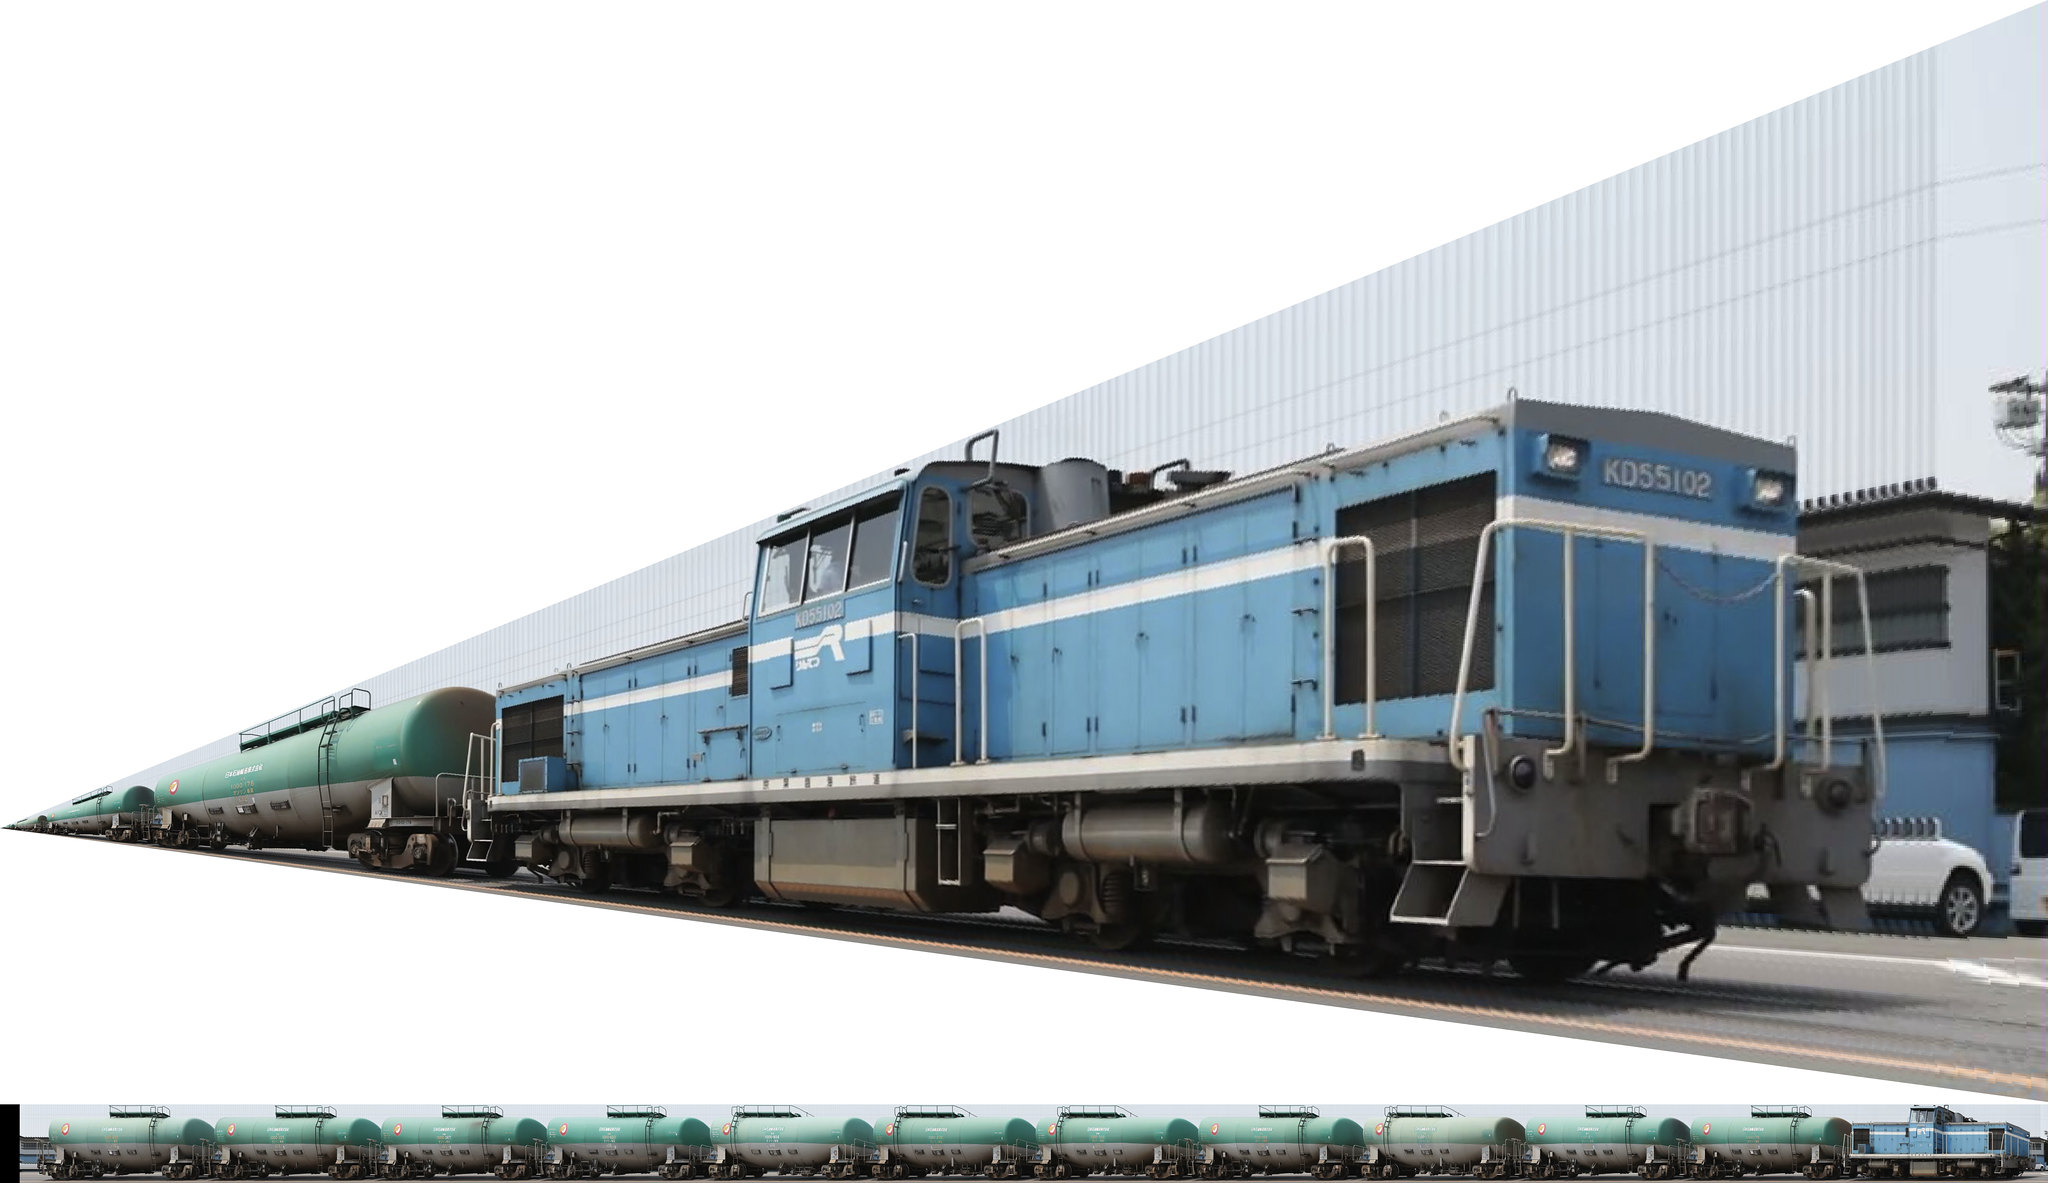
\includegraphics[width=\linewidth]{figures/example-1.jpg}
        \caption{This is a random figure added here}
    \label{fig:myRNDFig}
\end{figure}

Another thing that you might be interested in changing is the separation between paragraphs. There is a comment in the dissertation.cls with brief instructions on how to change that! Specifically, you are interested in changing this \textit{\textbackslash{setlength}\{\textbackslash{parskip}\}\{size\_em\}}. \textbf{OBS!} This might force you to change the many \textit{\textbackslash{vspace}\{value\}} that exists around all the class. 

\subsubsection{Deeper level}

This is the maximum level you should use, it is not too common to use deeper levels such as subsubsubsection as it can be observed in Table~\ref{table:sectionKnowledge} or~\cref{table:sectionKnowledge}.

\blindtext

\begin{table}
\begin{center}
\begin{tabular}{lccccc}
\hline
\rule{0pt}{12pt}
True Information&paper&$\Diamond$&$\Box$&$\bigtriangleup$ 
\\ 
\hline
\\[-6pt]
No & Paper 1 & 3 & 3 & 0 \\ 
Noup & Paper 2 & 3 & 3 & 0 \\ 
No & Paper 3 & 2 & 7 & 0 \\ 
Nah & Paper 4 & 5 & 3 & 0 \\ 
No & Paper 5 & 4 & 1 & 0 \\ 
Noup & Paper 6 & 5 & 0 & You wish \\ 
\hline
\\[-6pt]
\multicolumn{6}{l}{$\Diamond$ subsections\ \
$\Box$ subsubsections\ \
$\bigtriangleup$ subsubsubsections}
\end{tabular}
{\caption{Non-extensive and non-real table of papers that actually use different levels of sections. The information in this table could not be more fake so do not consider for your study :)\dots{} You can use this to create your tables if wanted: https://www.tablesgenerator.com/}\label{table:sectionKnowledge}}
\end{center}
\end{table}

However, if you really need subsubsubsections, then you can use the following:

\paragraph{This is a new subsubsubsection}
You define a subsubsubsection with the command \textit{\textbackslash paragraph} but normally you wouldn't need a subsubsubsection. 

\blindtext
\blindtext
\section{INTRODUCTION} \normalfont 
\label{sec:intro}
% \addcontentsline{toc}{section}{\nameref{sec:intro}}

%\epigraph{\textit{During the first three millennia, the Earthmen complained a lot.}}{John McCarthy}

% \setlength{\epigraphwidth}{3.5in} 
% \epigraph{\textit{There's a difference between knowing the path and walking the path.}}{Morpheus, The Matrix}


% \setlength{\epigraphwidth}{3in} 
% \epigraph{\textit{We can only see a short distance ahead, but we can see plenty there
% that needs to be done.}}{Alan M. Turing, Computing Machinery and Intelligence}

\setlength{\epigraphwidth}{4in} 
\epigraph{\textit{We all test the rules, and consider bending them; even a saint can appreciate science fiction. We add constraints [...] to see what happens then. We seek the imposed constraints [...] and try to overcome them by changing the rules. We follow up hunches [...], and - sometimes - break out of dead-ends. Some people even make a living out of pushing the existing rules to their limits, finding all the computational 'cans' that exist: creative tax-lawyers call them loopholes (and creative tax-legislators close them).}}{Margaret Boden \\ The Creative Mind: Myths and Mechanisms, pp. 58}

% \begin{dissQuote}{\~{}John McCarthy}
%     During the first three millennia, the Earthmen complained a lot.
% \end{dissQuote}

% \subsection{Tools}
% John McCarthy was spot on, as we humans, are a main source of complain. Nevertheless, such complains makes us strive and search for solutions and better approaches to cope with our needs and objectives. Ironically, we would end up complaining about it, restarting the loop.

\setlength{\parindent}{0.0em}

%John McCarthy was spot on, as we humans are a major source of complaint. Nevertheless, such complaints make us strive and search for solutions and better approaches to cope with our needs and objectives. Ironically, we would end up complaining about it, restarting the loop.

%Indeed Morpheus, there is a big difference between both! 

%We are all creative creatures 



%Look, we all want to feel special but the truth is, everyone is creative. Creativity is a human quality that exists in every single one of us. The degree of your or anyone else’s creativity doesn’t depend on an innate quality but rather on how hard you work.

%You could be as talented as Pablo Picasso, but if you don’t pump out the product, who cares? Your creativity is worthless

%While this might make people who have failed out creative fields (read: didn’t work hard enough) feel better, creativity is not something that a person is born with.

%Jory MacKay points out in his piece on Crew that not only is creativity taught in colleges and universities all over the world, but you can actually train your own brain to be more creative simply by doing creative work over a long period of time.

%If creativity was something we were just innately born with, that just wouldn’t be true

%Creativity

% Creativity is ``... the ability to produce work that is both novel (i.e., original, unexpected) and appropriate (i.e., useful, adaptive concerning task constraints)~\cite{sternberg_concept_1999}''. But what does that really means?

% \setlength{\parindent}{0.9em}

%and this happens all the time.

% Creativity is an outstanding ability that we possess. Some believe that they are not creative creatures, but in reality, and being candid about it, we are all creative and creative actions are taken all the time. We are all confronted with challenges and situations that require us to be creative on how we approach them. Whether this means being creative for artistic purposes such as painting or developing games, or to question your field and write a dissertation in political science, or to create variations on how to write your name; these all require creativity. Creativity varies on the task, process, outcome, and personal perception, which might be why people feel as non-creative~\cite{kaufman_beyond_2009}. Nevertheless, creativity as our other abilities, can be refined, developed, and fostered. 

% On the other hand, \textit{Computational Creativity} is the study of computational systems that demonstrate some human-like creative behaviors~\cite{colton_computational_2012}. We can imagine these as systems that can write stories~\cite{perez_y_perez_mexica_2001}, design games~\cite{cook_angelina_2016}, or SOMETHING MORE BASIC!. 

% Creativity is instrumental for the everyday life, exploration of ideas, and problem solving. Game design is a creative task that requires multi

% \begin{retQuestion}{}
%  How can we create tools that no longer behave just as aid to support our work but can collaborate with us, to some extent, in the same way as human collaboration functions? 
% \end{retQuestion}

% This thesis focuses on how game design related tasks such as the creation of game facets or designers' design process could be explored through Human-AI collaborative tools. While Procedural Content Generation algorithms could be employed by themselves for automated game design~\cite{nelson_towards_2007,cook_software_2020,cook_getting_2020}, this thesis takes a different approach and explores game design; and the creative, organizational, and collaborative tasks that encompass that; through Human-AI collaboration. Through this, we focus on fostering, enhancing, and augmenting human's capabilities such as creativity and adaptability 

% this thesis focuses on exploring multiple approaches for Human-AI collaboration. The goal is to develop systems and algorithms representing a computational designer to collaborate in the creation of content with a human designer. Tasks that could not only be assisted by AI but rather AI could be a \emph{colleague} in the design process. To tackle these shared tasks, a mutual feedback loop could be established, whereby AI and humans could inspire each other to explore unknown areas in the design landscape and reach better and more creative solutions.

% Using these tools 

% This thesis focuses on exploring how, through Human-AI collaborative tools, it would be possible to foster, enhance, and augment human's capabilities such as creativity. We explore this 

% Creativity is ``the ability to produce work that is both novel (i.e., original, unexpected) and appropriate (i.e., useful, adaptive concerning task constraints)~\cite{Sternberg1999-CreativityConcept}''. How creative processes occur, how an individual might come up with novel ideas, or how to assess creativity is very much an open research area~\cite{sternberg1999-handbookCreativity,boden2004-creative,Sternberg2005-creativityCreativities,Csikszentmihalyi97-Creativity}. Moreover,~\acrlong{cc} is a multidisciplinary field that studies computational systems that demonstrate human-like creative behaviors~\cite{Colton2012-CC}. As a multidisciplinary field,~\acrshort{cc} is not only interested in the algorithms or the outcome; it also aims to study the creative process and psychological causes of creative behaviors. Thus, through~\acrshort{cc}, some core concepts and research areas in creativity can be addressed. For instance, in \textit{the Creative Mind: Myths and Mechanism}, Boden studies and analyzes \emph{Creativity} and \emph{creative behaviors} with the use and help of~\acrshort{ai} through the lenses of~\acrlong{cc}. Boden discusses three forms of creativity: \textit{combinatorial}: combining existing knowledge in unfamiliar ways to produce new artifacts; \textit{exploratory}: exploring the conceptual space to encounter possible ideas;~\textit{transformational}: transforming the conceptual space, the imposed constraints, and the encountered ideas~\cite{boden2004-creative}.

% Within~\acrshort{cc}, games have been proposed as the optimal artifact to create to test the creative-like abilities of a~\acrshort{cc} system, since games are \emph{content-intensive}, \emph{multi-faceted content}, and should be~\emph{interacted with and experienced}~\cite{Liapis2014-gameCreativity}. As described above, game content relates to the main facets that represent any game: audio, visuals, narrative, levels, rules, and gameplay~\cite{Liapis2019-OrchestratingGames}. Thus, creating systems that develop, to some extent, games poses an interesting application and challenge for~\acrshort{cc}, which can address some of the core questions in~\acrshort{cc}. For instance, investigating the creative process not only to create one type of content but the arrangement of such in a harmonious way as a team of humans creatively does, or the assessment of such content.



%, and we areall the time. 

% \setlength{\parindent}{0.9em}

Since the dawn of time, we humans have been searching [and in need] for tools to develop our ideas or execute mundane objectives. As time and technology advanced, more sophisticated types of assistance emerged to cope with humans' needs, such as vehicles to traverse longer paths or ways to facilitate writing. With the invention of hardware and software, its ubiquity, and the raise of~\acrfull{ai}, a new path for human assistance opened up. Tools that were used to facilitate our work or assist us into doing repetitive work, could now provide advance assistance with smarter tools that allows us to work more efficiently. However, tools that assist us in our tasks are not the only key factor; the collaboration between humans has remained virtually unchanged as an essential way to move forward and to develop new experiences. Not only to achieve greater objectives as a group but also to develop as individuals. While the current tools to support humans' work and creative output are valuable in many ways; this raises an essential question that holistically motivates this thesis:

\setlength{\parindent}{0.9em}

\begin{retQuestion}{}
 How can we create tools that no longer behave just as aid to support our work but can collaborate with us, to some extent, in the same way as human collaboration functions? 
\end{retQuestion}

This thesis focuses on how game design related tasks such as the creation of game facets or designers' design process could be explored through Human-AI collaborative tools. While Procedural Content Generation algorithms could be employed for automated game design~\cite{nelson_towards_2007,cook_software_2020,cook_getting_2020}, this thesis takes a different approach and explores game design; and the creative, organizational, and collaborative tasks that encompass that; through Human-AI collaboration. We focus on fostering, enhancing, and augmenting human abilities such as creativity. Multiple approaches, systems, and algorithms representing a computational designer to collaborate in the creation of content with a human designer are developed. These tasks could not only be assisted by AI, but rather AI could be a \emph{colleague} in the design process. To tackle these shared tasks, a mutual feedback loop could be established, whereby AI and humans could inspire each other to explore unknown areas in the design landscape and reach better and more creative solutions.

% Since the dawn of time, we humans have been searching [and in need] for tools to develop our ideas or execute mundane objectives. As time and technology advanced, more sophisticated types of assistance emerged to cope with humans' needs, such as vehicles to traverse longer paths or ways to facilitate writing. With the invention of hardware and software, its ubiquity, and the raise of~\acrfull{ai}, a new path for human assistance opened up. Tools that were used to facilitate our work by doing impossible things for us, e.g., move 500 km in a day, or assist us into doing repetitive work, could now provide advance assistance with smart tools that allows us to work and explore differently and more efficiently (Unity, 2005; Photoshop, 1990). However, tools that assist us in our tasks are not the only key factor; the collaboration between humans has remained virtually unchanged as an essential way to move forward and to develop new experiences. Not only to achieve greater objectives as a group but also to develop as individuals. While the current tools to support humans' work and creative output are valuable and helpful in many ways; this raises an essential question that holistically motivates and drives this thesis:


% Rather than having tools that facilitate our work by doing impossible things for us, e.g., move 500 km in a day, or assist us into doing repetitive work, they can now provide advance assistance with smart tools that allows us to work and explore differently and more efficiently (Unity, 2005; Photoshop, 1990).

% \begin{retQuestion}{}
%  How can we create tools that no longer behave just as aid to support our work but can collaborate with us, to some extent, in the same way as human collaboration functions? 
% \end{retQuestion}

% This thesis focuses on exploring multiple approaches for Human-AI collaboration. The goal is to develop systems and algorithms representing a computational designer to collaborate in the creation of content with a human designer. Tasks that could not only be assisted by AI but rather AI could be a \emph{colleague} in the design process. To tackle these shared tasks, a mutual feedback loop could be established, whereby AI and humans could inspire each other to explore unknown areas in the design landscape and reach better and more creative solutions.

\subsection{Problem Statement} \label{sec:problemst}

The proposed question is not new and has been approached by different disciplines, under the~\acrfull{mi} paradigm.~\acrshort{mi} refers to the collaboration between \emph{human} and \emph{computer} where both have some proactive initiative to solve some task.~\acrshort{mi} can be seen as a multi-agent collaboration scenario, where the interaction should be flexible, allowing for a continuous negotiation of initiative and leverage on each other's strengths to solve a task~\cite{allen_mixed-initiative_1999}. \emph{Initiative} was described by Novick and Sulton as a multi-factor model that combines: choosing the task, choosing the agent in control and how the interaction is established, and choosing the expected outcome from the collaboration~\cite{novick_what_1997}. 

Moreover, Horvitz discussed such a question in terms of Intelligent User Interfaces~\cite{birnbaum_compelling_1997}, describing mixed-initiative systems and interfaces as a more natural collaboration in a user interface that emerges from intertwining human control and manipulation, and automation~\cite{horvitz_uncertainty_1999}. Horvitz presented several principles of mixed-initiative interaction and its challenges, many of which still exist~\cite{horvitz_principles_1999}, mainly describing this interaction as conversation systems between AI and humans~\cite{horvitz_computational_1999}. Moreover, Yannakakis et al. introduced the~\acrfull{micc} paradigm for the co-creation of creative content, where both AI and humans alternate in the initiative to co-design and solve tasks~\cite{yannakakis_mixed-initiative_2014}. Their work describes key findings and discussions for how MI-CC does not only help human designers solve tasks, but also fosters their creativity through an interactive feedback loop and lateral thinking~\cite{liapis_can_2016,liapis_computational_2014,alvarez_fostering_2018}.


% ~\cite{Liapis2016-CanComputersFosterCreativity,Liapis2014-gameCreativity,Alvarez2018}. 

%Paramount is the role of the computer agent in this interaction, as it would help establish the boundaries of the interaction, what is expected, and how creativity could be fostered. Lubart analyzed this interaction and examined the different ways computers could be involved in creative work to promote creativity. In his work, he proposed four roles: \emph{computer as nanny}: management of creative work; \emph{computer as pen-pal}: communication service between collaborators; \emph{computer as coach}: Using creative enhancement techniques; and \emph{computer as colleague}: partnership between computer and humans~\cite{lubart_how_2005}. Recently, this was explored by Guzdial et al., where designers perceived the AI collaborator with more or less value depending on their desired role for the AI, varying between: \emph{friend}, \emph{collaborator}, \emph{student}, or \emph{manager}~\cite{guzdial_friend_2019}.

Nevertheless, this collaborative approach raises an \emph{initiative} challenge for either agent: Which agent should have the initiative at different stages of the development and over the goal? The question reflects the diffuseness of the challenge and situation, as many factors need to be considered before appropriately indicating this. At the very least, some could say that depending on the task to be performed and the expertise of both, either would clearly be the one taking the development initiative. Whereas others would position the human as the one always in control. Yet, even with a clear answer, what happens in creative tasks to the expressivity of one of the sides due to the other taking the initiative? 

Furthermore, one context where the~\acrshort{mi} paradigm would be very beneficial is games. Games, either digital or tabletop, are created through a complex creative process that couple together many different creative facets in different ways. Games contain a large amount of creative content carefully combined and intertwined to craft specific experiences, with the addition of rules that dictate how a player is to interact with it. In contrast with other creative content, games are multifaceted, content-intensive, and should be interacted, experienced, and enjoyed by others, which also creates a complex subjective task~\cite{liapis_computational_2014}. Usually, games are developed by more than a person (although many exceptions exist~\cite{minecraft,undertale,stardewvalley}), reaching to hundreds and thousands of developers, with each developer specialized in different areas such as gameplay, AI, animation, concept art, etc. Each creates a specific part of the game and the content through collaboration and following a road map~\cite[Chapter~14]{fullerton_game_2004}. However, no matter the team's size and talent, the fact remains that developing games is a hard challenge~\cite{blow_game_2004}. As technology advances, the requirements increase substantially for any game facet, coupled with the users' increase demand, the higher competitiveness in the market, and the launch of many more platforms~\cite{washburn_jr_what_2016}.

\acrfull{pcg} is a field within computational intelligence in games, that focuses on the use of algorithms to create game content~\cite{yannakakis_artificial_2018}.~\acrshort{pcg} algorithms have been used to aid in the creation of a plethora of games such as No Man Sky~\cite{nomansky}, Spelunky~\cite{spelunky}, or Minecraft~\cite{minecraft}, to the extent that~\acrshort{pcg} and~\acrshort{ai} have enabled experiences and interactions that were not possible before~\cite{aidungeon,rogue,elite}. Moreover, as one of the properties of~\acrshort{pcg} is to increase replayability by creating an abundance of well-made content~\cite{shaker_procedural_2016}, games are not the only beneficiaries of~\acrshort{pcg} methods. For instance, they have the opportunity to be used to increase the generality of~\acrfull{ml} approaches~\cite{risi_increasing_2020}, or a step towards open-endedness~\acrfull{ec}~\cite{clune_ai-gas_2019}. 

% In this thesis, the focus is on exploring multiple approaches for the collaboration between AI and humans to co-create game content in a~\acrlong{micc} paradigm. The goal is to develop systems, techniques, and algorithms representing a [creative] computational designer to tackle the different tasks in game design and development. Tasks that could not only be assisted by AI but rather AI could be a \emph{colleague} in the creative process. To tackle these shared tasks, a mutual feedback loop could be established, whereby AI and humans could inspire each other to explore unknown areas in the design landscape and reach better and more creative solutions.

% \subsection{Problem Statement} \label{sec:problemst}

% Furthermore, there has been a significant effort to analyze the possibilities of such a collaboration, resulting in multiple Ph.D. theses exploring and focusing on different aspects of~\acrshort{mi}~\cite{SmithPhD,LiapisPhD,ComptonPhD,GuzdialPhD,MachadoPhD}. Thus, there is a growing interest in how to establish mixed-initiative interactions and new ways of humans and AI to collaborate. Earlier work focused on tools that supported the work of humans, combining the strengths of both. Later on, research demonstrated that such interaction could enable the completion of tasks not previously able to be done by either alone, and enable creative work to be stimulated. 

Moreover, in design and creative tasks such as games, the designer usually has intentions in what they are creating and goals that they want to achieve with their design. Thus, to enable deeper~\acrshort{mi} levels to co-create content, some control mechanisms with a varying degree of control over the algorithms might be necessary for the designer. Through this, the designer could direct or constraint the generated content by the computational designer and oversee that it is within their intentions and goals. In this case, each agent's control and expressive properties are at the expense of the other agents, as it constrains the space of possibilities~\cite{baldwin_mixed-initiative_2017}. This is especially relevant when the aim is a creative work such as games, where the creative expression needs to be fostered~\cite{alvarez_fostering_2018}. Yet, it becomes particularly challenging when using mixed-initiative methods, where smart approaches need to be in place for a natural conversation and successful collaboration. The more control is given, the more constraint it exists, but is this a problem? Is it inevitable? Boden explains it conspicuously ``...  We [humans] seek the imposed constraints [...], and try to overcome them by changing the rules.~\cite{boden_creative_2004}''. Constraints limit the space, and as a consequence, they are overcome by encountering creative solutions.

For this interaction to be complete, the human needs to understand the AI's behavior through interpretable and explainable models and systems, and the AI needs to recognize and interpret the intentions of the humans seamlessly as they create their content. The former is the focus of~\emph{Interpretable} and \emph{Explainable AI}, which seeks to create or adapt models and systems for a better workflow between humans and AI, where humans could understand the AI's decision process to enable trust relationships and reach deeper interactions~\cite{zhu_explainable_2018,doshi-velez_considerations_2018,adadi_peeking_2018}. The latter would mean that the AI could adapt its behavior and functionality to the needs, expertise, and workflow of individual designers or a specific group of designers. To do so, the AI must analyze several design processes, such as the designer's preferences, styles, and goals, which holistically is called \emph{Designer Modeling}~\cite{liapis_designer_2013,liapis_designer_2014}. How to create these models and use them to develop adapted experiences is a complex challenge, and understanding the implications of its usability in the control-expressive properties, as well as other consequences, is not trivial.

To explore this, the main body of work presented in this dissertation is applied and evaluated through the~\acrfull{edd}, a~\acrlong{micc} system, where designers can create levels and narrative elements, such as quests or objectives for adventure and dungeon crawler games such as Zelda~\cite{tloz} or The Binding of Isaac~\cite{bindingISAAC}. In~\acrshort{edd}, the human designer can, on the one hand, quickly create interconnected rooms forming a dungeon to be experienced by players. Meanwhile, the computational designer collaborates by providing suggestions using different algorithms and following multiple heuristics. On the other hand, the human designer can compose quests using the level information and the overarching narrative structure. 

%The human designer can interact in several ways with the computational designer so that this adapts its output to whatever goal the human designer has, while still providing a diverse amount of alternatives and different experiences to the human designer.

% Interactive systems can help humans complete creative tasks that are tedious or require substantial human workload. Such creative tasks could be as simple as drafting a grammar corrected text (e.g., MS Word), to more complex scenarios such as creating visual artifacts (e.g., Adobe Photoshop) or designing entire video games (e.g., Unity Engine).~\acrlong{micc} is a paradigm within~\acrshort{pcg}, where both human and AI proactively collaborate to co-create and co-design games or creative content. Through~\acrshort{micc}, the potential of interactive tools increases substantially.~\acrshort{micc} enables a new way of tackling creative tasks engaging in-depth humans and AI rather than just helping humans to complete tasks and reduce their workload. Furthermore, enabling a mutual feedback loop could also foster both participants' creativity, create adaptive experiences for the users, or focus on achieving tasks with better and interesting results in a hybrid format. Multiple approaches have been proposed as alternatives for creating systems that model the interaction between AI and humans to create game content, and that use different techniques to study such interactions and its implications~\cite{Alvarez2020-ICMAPE,smith_tanagra:_2011,Liapis2013-sentientsketchbook,charity2020baba}. 



% In this thesis, the focus is on exploring multiple approaches for the collaboration between AI and humans to co-create game content in an~\acrlong{micc} paradigm. The goal is to develop systems, techniques, and algorithms representing a [creative] computational designer to tackle the different tasks in game design and development. Tasks that could not only be assisted by AI but rather AI could be a \emph{colleague} in the creative process. To tackle these shared tasks, a mutual feedback loop could be established, whereby AI and humans could inspire each other to explore unknown areas in the design landscape and reach better and more creative solutions.



% Nevertheless, this collaborative approach divided into human control and AI automation as presented by Horvitz~\cite{Horvitz99-mixedInit} with multiple initiatives at different points of the development as discussed by Yannakakis et al.~\cite{yannakakis2014micc}, raises a controllability challenge for either actor: Which of the two should have the control at different steps of the development and over the goal? There is no real answer since it is very diffuse, and many factors need to be consider before appropriately indicating this. At the very least, some could say that depending on the task to be performed and the expertise of both, one or the other would clearly be the one in control of the development, whereas others would clearly position the human as the one in control. Yet, even if the answer would be clear, what happens to the expressivity of one of the sides as a consequence of the other controlling? The more control is given, the more constraint it exist, but is this a problem? Is it inevitable? At last, Boden explains it quite clear ´´...  We seek the imposed constraints [...], and try to overcome them by changing the rules.''~\cite{boden2004-creative}

% Point out that this collaborative search for human control and AI automation with multiple initiatives at different points of the development, give raise to a controllability challenge for either two actors. Moreover, when we discuss content generation 

% If the aim of this research area is to push harder for mixed-initiative tools, where more autonomy is given to the AI, and for humans to consider the AI as a collaborator as described by Lubart~\cite{LUBART2005-computerPartners} and Guzdial et al.~\cite{guzdial2019friend} that can be taken serious and used its input as a key factor in the development of any type of content. Then we are required to develop AIs and tools that not only provides interesting and valuable input to the human, but also adaptive experiences that 


% This collaboration may take different forms as studied by Lubbart~\cite{LUBART2005-computerPartners}, and recently explored by Guzdial et al.~\cite{guzdial2019friend}.


% \subsection{Computational Creativity and Games}

% Games, either digital or tabletop, are created through a complex creative process that couple together many different creative facets in different ways. Games contain a large amount of creative content carefully combined and intertwined to craft specific experiences, with the addition of rules that dictate how a player is to interact with it. In contrast with other creative content, games are multifaceted, content-intensive, and should be interacted, experienced, and enjoyed by others, which also creates a complex subjective task~\cite{Liapis2014-gameCreativity}. Usually, games are developed by more than a person (although many exceptions exist~\cite{minecraft,undertale,stardewvalley}), reaching to hundreds and thousands of developers, with each developer specialized in different areas such as gameplay, AI, animation, concept art, etc. Each creates a specific part of the game and the content through collaboration and following a road map~\cite[Chapter~14]{fullerton2004-gamedesign}. However, no matter the team's size and talent, the fact remains that developing games is a hard challenge~\cite{Blow2004-gamesHard}. As technology advances, the requirements increase substantially for any game facet, coupled with the users' increase demand, the higher competitiveness in the market, and the launch of many more platforms~\cite{Washburn2016-gamesPostmorten}.

% Moreover,~\acrfull{cc} is one of the grand challenges of~\acrshort{ai}, where the quest is to study, develop, and build computational systems that demonstrate creative behaviors and can create multiple types of artifacts such as games or stories~\cite{Colton2012-CC}. Within the various content that can be created, games offer a unique property that distances them from other creative outputs, making them more interesting to be analyzed and experimented on than others~\cite{Liapis2014-gameCreativity}. They offer a set of intertwined facets that represent any game: audio, visuals, narrative, levels, rules, and gameplay~\cite{Liapis2019-OrchestratingGames}, whereas other creative content focuses almost exclusively on a single-aspect, e.g., music or dance. However, single-aspect creative content has its own set of challenges. For instance, creating a system that creates music could mean creating each separated instrument, music sheet, arrangements, etc~\cite{HooverPhD}. Furthermore, Games must be interacted with and enjoyed by others than the developers, and the fact that these facets must naturally fit each other poses them as a very exciting application to be researched and developed within the~\acrshort{cc} field.

% \acrfull{pcg} is a field within computational intelligence in games, that focuses on the use of algorithms to create game content~\cite{Yannakakis2018}.~\acrshort{pcg} algorithms have been used to aid in the creation of a plethora of games such as No Man Sky~\cite{nomansky}, Spelunky~\cite{spelunky}, or Minecraft~\cite{minecraft}, to the extent that~\acrshort{pcg} and~\acrshort{ai} have enabled experiences and interactions that were not possible before~\cite{aidungeon,rogue,elite}. Moreover, as one of the properties of~\acrshort{pcg} is to increase replayability by creating an abundance of well-made content~\cite{shaker_procedural_2016}, games are not the only beneficiaries of~\acrshort{pcg} methods. For instance, they have the opportunity to be used to increase the generality of~\acrfull{ml} approaches~\cite{Risi2020-pcgGeneralityML}, or a step towards open-endedness~\acrfull{ec}~\cite{clune2019-aigas}. 

% Furthermore, several computational designers and systems have been developed to create complete games such as Angelina~\cite{Cook2016-Angelina1}, Ludi~\cite{Browne2010-ludii}, a system to create card games~\cite{font2013-GenCardGames}, or a system that uses data from Wikipedia to create mystery games~\cite{barros2018-DATAeinstein}. Automated game design, as developed in those systems, show interesting and important advancements towards~\acrshort{cc} systems. However, not including the human designer creates constraints, challenges, and limitations in these systems, such as modeling fun, enjoyment, and interaction. Another interesting and promising path to explore is the~\acrlong{micc} paradigm within~\acrshort{pcg}, combining both~\acrshort{ai} and humans to co-create the game content, which is the focus of this thesis.

% \subsection{Problem Statement} \label{sec:problemst}

% Interactive systems can help humans complete creative tasks that are tedious or require substantial human workload. Such creative tasks could be as simple as drafting a grammar corrected text (e.g., MS Word), to more complex scenarios such as creating visual artifacts (e.g., Adobe Photoshop) or designing entire video games (e.g., Unity Engine).~\acrlong{micc} is a paradigm within~\acrshort{pcg}, where both human and AI proactively collaborate to co-create and co-design games or creative content. Through~\acrshort{micc}, the potential of interactive tools increases substantially.~\acrshort{micc} enables a new way of tackling creative tasks engaging in-depth humans and AI rather than just helping humans to complete tasks and reduce their workload. Furthermore, enabling a mutual feedback loop could also foster both participants' creativity, create adaptive experiences for the users, or focus on achieving tasks with better and interesting results in a hybrid format. Multiple approaches have been proposed as alternatives for creating systems that model the interaction between AI and humans to create game content, and that use different techniques to study such interactions and its implications~\cite{Alvarez2020-ICMAPE,smith_tanagra:_2011,Liapis2013-sentientsketchbook,charity2020baba}. 

% Nevertheless, this collaborative approach divided into human control and automation~\cite{Horvitz99-mixedInit} with multiple initiatives~\cite{Allen99-MIinteraction,novick97-mixedInit}, and whereas it could foster humans' creativity~\cite{yannakakis2014micc}, raises an \emph{initiative} challenge for either agent: Which agent should have the initiative at different stages of the development and over the goal? The question reflects the diffuseness of the challenge and situation, as many factors need to be considered before appropriately indicating this. At the very least, some could say that depending on the task to be performed and the expertise of both, either would clearly be the one taking the development initiative. Whereas others would position the human as the one always in control. Yet, even with a clear answer, what happens in creative tasks to the expressivity of one of the sides due to the other taking the initiative? 

% Moreover, in design and creative tasks, the designer usually has intentions in what they are creating and goals that they want to achieve with their design. Thus, to enable deeper~\acrshort{mi} levels to co-create content, some control mechanisms with a varying degree of control over the algorithms might be necessary for the designer. Through this, the designer could direct or constraint the generated content by the computational designer and oversee that it is within their intentions and goals. In this case, each agent's control and expressive properties are at the expense of the other agents, as it constrains the space of possibilities~\cite{Baldwin2017}. This is especially relevant when the aim is a creative work such as games, where the creative expression needs to be fostered~\cite{Alvarez2018}. Yet, it becomes particularly challenging when using mixed-initiative methods, where smart approaches need to be in place for a natural conversation and successful collaboration. The more control is given, the more constraint it exists, but is this a problem? Is it inevitable? Boden explains it conspicuously ``...  We [humans] seek the imposed constraints [...], and try to overcome them by changing the rules.~\cite{boden2004-creative}''. Constraints limit the space, and as a consequence, they are overcome by encountering creative solutions.

% Furthermore, for this interaction to be fully fleshed, the human needs to understand the AI's behavior through interpretable and explainable models and systems, and the AI needs to recognize and interpret the intentions of the humans seamlessly as they create their content. The former is the focus of~\emph{Interpretable} and \emph{Explainable AI}, which seeks to create or adapt models and systems for a better workflow between humans and AI, where humans could understand the AI's decision process to enable trust relationships and reach deeper interactions~\cite{Zhu2018-XAIDesignersMICC,Doshi-Velez2018,adadi2018peeking}. The latter would mean that the AI could adapt its behavior and functionality to the needs, expertise, and workflow of individual designers or a specific group of designers. To do so, the AI must analyze several design processes, such as the designer's preferences, styles, and goals, which holistically is called \emph{Designer Modeling}~\cite{Liapis2013-designerModel,Liapis2014-designerModelImpl}. How to create these models and use them to develop adapted experiences is a complex challenge, and understanding the implications of its usability in the control-expressive properties, as well as other consequences, is not trivial.

% In this thesis, the focus is on exploring multiple approaches for the collaboration between AI and humans to co-create game content in an~\acrlong{micc} paradigm. The goal is to develop systems, techniques, and algorithms representing a [creative] computational designer to tackle the different tasks in game design and development. Tasks that could not only be assisted by AI but rather AI could be a \emph{colleague} in the creative process. To tackle these shared tasks, a mutual feedback loop could be established, whereby AI and humans could inspire each other to explore unknown areas in the design landscape and reach better and more creative solutions.

% To explore this, the main body of work presented in this dissertation is applied and evaluated through the~\acrfull{edd}, a~\acrlong{micc} system, where designers can create levels for rogue-like and adventure type of game such as Zelda~\cite{tloz} or The Binding of Isaac~\cite{bindingISAAC}. In~\acrshort{edd}, the human designer can quickly create interconnected rooms forming a dungeon to be experienced by players. Meanwhile, the computational designer collaborates by providing suggestions using different algorithms and following multiple heuristics. The human designer can interact in several ways with the computational designer so that this adapts its output to whatever goal the human designer has, while still providing a diverse amount of alternatives and different experiences to the human designer.

\subsection{Research Questions} \label{sec:RQS}

As motivated thus far, this thesis focuses on exploring different approaches for procedurally generating content for games, specifically through the~\acrshort{micc} paradigm, where a human designer collaborates with an underlying AI to create creative content. Exploring the role of \emph{computers as colleagues} as defined by Lubart~\cite{lubart_how_2005}, this thesis delves into the use of~\acrshort{micc} tools and the multiple properties that emerge from the dynamic interaction between AI and Humans. The aim is to understand how we can enable a rich, fruitful, and better feedback loop in these types of tools using and developing novel AI techniques in the field of~\acrlong{ec} and~\acrlong{ml} to improve the interaction and create adapted experiences. The thesis also analyzes and studies the requirements, challenges, and benefits of enabling in-depth collaboration, tailored experiences, the properties that emerge (some seemingly competing properties), and their dynamics. Therefore, this thesis aims at addressing, discussing, and exploring the following research questions: 

% \begin{retQuestion}{}
% %   \textbf{RQ1.} How can we use and implement different algorithms into a mixed-initiative approach to help designers produce high-quality content and foster their creativity? 
   
% %   \textbf{RQ1.} How can we use, implement, and combine quality-diversity algorithms and  different algorithms into a mixed-initiative approach to help designers produce high-quality content and foster their creativity? 
   
%   \textbf{RQ1.} How can we generate content in tandem with designers in a mixed-initiative system to help them produce high-quality content and foster their creativity?
   
%       \begin{retQuestion}{}
%         \textbf{RQ1.1} How can we use and integrate quality-diversity algorithms into the mixed-initiative system? 
%         % into a mixed-initiative approach in order to generate high-performing and diverse content for designers?
%     \end{retQuestion}
   
%   \begin{retQuestion}{}
%         \textbf{RQ1.2} How can we use and integrate grammars into the mixed-initiative system?
        
% %         How can we integrate patterns for the generation of different type of content  
%     \end{retQuestion}
    
%     \begin{retQuestion}{}
%         \textbf{RQ1.3} To what extent can designers control the algorithms to steer and adapt the generated content?
%     \end{retQuestion}
%     %   How can we use and integrate quality-diversity algorithms into a mixed-initiative approach to help designers produce high-quality content and foster their creativity while allowing them to control, to a certain extent, the generated content?
% \end{retQuestion}

\begin{retQuestion}{}
   
   \textbf{RQ1.} How can we use and integrate multiple algorithms such as quality-diversity algorithms and grammars into a mixed-initiative approach to help designers produce high-quality content and foster their creativity while allowing them to control, to a certain extent, the generated content?
\end{retQuestion}


There are plenty of approaches and algorithms such as Evolutionary Computation, Machine Learning, or Wave Function Collapse that have been used to generate content as it will be discussed in the background chapter (sec.~\ref{background}). In this thesis, we are interested in exploring these algorithms and approaches, particularly quality-diversity algorithms, pattern-based systems, grammar systems and their use as encoding representation in MI-CC systems. In these MI-CC systems, the aim is to have more controllable yet expressive generators, and at the same time explore how they can be used to foster the designers' creativity and establish better human-AI collaboration and interactions.

\acrfull{qd} algorithms are a relatively new family of algorithms, specifically aimed at tasks and environments that require the strengths of convergence and divergence search~\cite{pugh_quality_2016}. Leveraging on~\acrshort{qd} algorithms to search for a surfeit of heterogeneous content while not losing sight of the content's quality could enable~\acrshort{micc} systems to explore a big area of the generative space producing more diverse and high-quality solutions. Through this, the system could propose a higher range of diverse solutions to the user, aiming at fostering the creativity of the human designer~\cite{liapis_can_2016}. Thus, how to integrate~\acrshort{qd} algorithms in~\acrshort{micc} systems that need to take into account the human work to provide valuable input is a promising open research area and one that this thesis explores. However, it is paramount to understand how to effectively use~\acrshort{qd} algorithms in these systems to fully leverage their expressive power while providing control to human designers.

\begin{retQuestion}{}\sloppy
%   \textbf{RQ2.} How can we use gameplay, player, and designer data to understand better players' and designers' actions and behaviors to enhance their experiences?
   \textbf{RQ2.} How can we use player and designer data to better understand their behaviors and procedures to enhance and adapt~\acrlong{micc} systems?
   
%   understand better players' and designers' actions and behaviors to enhance their experiences?,
   
   
%   \textbf{RQ2.} What type of data is representative of player and designer 
   
%   How can we use gameplay, player, and designer data to understand better players' and designers' actions and behaviors to enhance their experiences?
\end{retQuestion}

Games and creative contexts are spaces where both players and designers can express themselves, producing data on how they both interact. Research areas such as Experience-driven PCG~\cite{yannakakis_experience-driven_2011}, player modeling~\cite{pedersen_modeling_2010,holmgard_automated_2019} or designer modeling~\cite{liapis_designer_2013}, explore the use of such data to understand particular users~\cite{liapis_designer_2013,drachen_player_2009,melhart_your_2019} and to improve and enhance the experiences of players and designer. Especially focusing on enabling adaptive experiences~\cite{hastings_evolving_2009} and more accurate heuristics~\cite{marino_empirical_2015,canossa_towards_2015,summerville_understanding_2017}. However, how to use the data (and even what to collect) is still an open research area, especially when applied to adaptive experiences for~\acrshort{micc} tools with only a few relevant examples~\cite{liapis_designer_2014,liapis_adapting_2012,halina_threshold_2022}. Furthermore, the importance of enhancing the experience of~\acrshort{micc} tools' users lies in the search for deeper understanding and collaboration between humans and~\acrshort{ai}, which could enable a better experience for both.

\begin{retQuestion}{}
   \textbf{RQ3.} How can we model different designers' procedures and use them as surrogate models to anticipate the designers' actions, produce content that better fits their requirements, and enhance the dynamic workflow of mixed-initiative tools?
   
    \begin{retQuestion}{}
        \textbf{RQ3.1} What trade-offs arise from modeling and using designer's procedures to steer the generation of content towards personalized content?
    \end{retQuestion}
   
   \begin{retQuestion}{}
        \textbf{RQ3.2} What constraints are created over the generative process when using designer models?
    \end{retQuestion}
   
\end{retQuestion}

The advantage of having the human and AI collaborating is analogous to humans collaborating, each one with their own set of strengths and weaknesses to reach greater objectives and develop each other. However, mixed-initiative collaboration requires both human and AI to understand each other and the goals that the human aim to reach~\cite{horvitz_principles_1999,novick_what_1997}. This creates a particular problem where the AI needs to identify certain processes and characteristics of the human. When employing~\acrshort{micc} to co-create games and creative artifacts; this translates to design processes, style, preferences, intentions, and goals. This thesis aims to explore how to model different designer procedures such as preference or style, using several~\acrlong{ml} methods, and how to best use these as surrogate models to produce better content and enhance designers' experience using~\acrshort{micc} systems.

RQ2 and RQ3 drive the research on how to gather and use different types of data, i.e., player and designer data, and whereas designer modeling could be used in the~\acrshort{micc} feedback loop to create adaptive experiences. Through RQ3.1 and RQ3.2, this thesis focuses on exploring the trade-offs of using designer modeling. Specifically, the interest lies in the challenges and benefits that designer modeling creates for the algorithms and designers, and the overall experience that the designer wants to create, i.e., the game. 

Moreover, the constraints that emerge from using these models as surrogate models to steer the content generation are not trivial to address and are essential to study to understand and analyze their effect and extent. Using these models will inevitably create constraints over the generation process as we aim to adapt the experience to each designer or group of designers. Therefore, RQ3.2 specifically aims at understanding: what are these constraints? What is constrained? And whether these constraints are positive or negative? 

\begin{retQuestion}{}
   \textbf{RQ4.} How can level design and narrative interact, act as constraints, be intertwined, and in general, have an active role affecting each other to produce a holistic system? 
   
    % \begin{retQuestion}{}
    %     \textbf{RQ4.1} What are the requirements and main factors needed to establish a relation between the level design and the narrative, and what are the criteria to evaluate the respective generated content? 
    % \end{retQuestion}
   
   \begin{retQuestion}{}
        \textbf{RQ4.1} What are the factors to be considered when implementing such a paradigm and system in a mixed-initiative application, where a designer will be able to interact with the content?
    \end{retQuestion}
    
    \begin{retQuestion}{}
        \textbf{RQ4.2} What are the effects of producing and using a holistic system for the creative process of a designer, and what challenges are imposed on computational creativity? 
    \end{retQuestion}
   
\end{retQuestion}

The intertwined, multi-faceted, and collaborative nature of games invites the exploration of how to generate different facets and how to intertwine them. Facets in a game are seldom produced in a vacuum, and the coherence of a game and cohesion of game content rely on these facets to be relevant and aligned with each other. The automatic generation of game content could follow a similar process, so the resulting content feels coherent, which has been categorized as Holistic PCG~\cite{liapis_orchestrating_2019,salge_generative_2018}. Usually, systems that generate several facets focus on a hierarchical and step-by-step process where each facet is generated successively and, at times, not relying on the other generated facets but rather on an overarching design goal. The generation of game facets could then have some feedback loop, where content generated in one facet has an effect on another, and vice-versa, generating content in unison, i.e., orchestrating game content.

Moreover, the importance of space or game worlds and narrative has been pointed out by previous research in different disciplines. For instance, Aarseth links the space to the quest in games, both dependant on each other~\cite{kishino_hunt_2005}. Ashmore and Nitsche present a similar point in relation to the games' interactivity as they discuss that a generated level without depth and context lacks interest for the final user~\cite{ashmore_quest_2007}, further discussed and related by Kybartas and Bidarra with a focus on story automation~\cite{kybartas_quinn_survey_2017}. Similarly, Dehn~\cite{dehn_story_1981} defines space (i.e., the world) as a post-hoc development and justification for authored events, while Lebowitz~\cite{lebowitz_creating_1983} argues for the opposite view, the story gives meaning to a created world. Looking at the narrative-space discussion from whichever angle and perspective, it is noticeable that one requires the other to develop fully and fruitfully. Therefore, the intertwined generation of both facets is a suitable first approach to holistic PCG, which this thesis explores. 

Nevertheless, there are several challenges when posing content generation as a multi-faceted and intertwined task, such as how to represent the content, what elements to use as constraints, or how to evaluate the generated content. Yet one of the objectives explored in this thesis is to add and combine this into an MI-CC system. This exacerbates the challenge, as human input and control become central, and we consider their input and initiative and the role of the AI in the system. Likewise, MI-CC challenges and considerations are extended, whereas the generated content must not only adapt and be relevant for the human (considering their input as well) but also maintain and adapt to other constraints from different facets. 
%Likewise, how the system would adapt and generate relevant content considering human input while maintaining other constraints is a 

%  as we consider human input and initiative, and the role the AI agent takes in the system.

% The goal in this thesis is then, to combine this into an MI-CC system. This exacerbates the challenge as we need to consider humn input in the system and how the system would be able to adaptand generate relevant content that is in a feedback loop based on what the designer is creating.

% Adding this into an MI-CC system exacerbates the challenge as we need to consider human input in the system and how the system would we abvle to adapt and generate relevant content that is in a feedback loop based on what the designer inputs and what the content in other facets is generated. 

% the multi-faceted generation of content brings a set of challenges 

% Nevertheless, this multi-faceted generation of content have 

% This is especially relevant in MI-CC as 


% , where Human and AI collaborate to create content and both

% There are several examples that focus on a tandem generation of content



%Games are



% \begin{retQuestion}{}
%   \textbf{RQ5.} How does the agency of the designer and the agency of the underlying AI-technology component in mixed-initiative approaches, and the interaction between both actors, affects the overall design process and the usefulness of mixed-initiative tools?
% \end{retQuestion}

% \blindtext

% Esto es lo que pone el study handbook sobre lo que debe contener la tesis para el final seminar: “Similar to the when the licentiate thesis is reviewed, all parts (cover paper and papers) of the manuscript shall be in place for the final seminar. These parts may not be fully processed; however, the cover paper must at least include research questions, contributions, methodology and a mapping between the research questions and the papers.”

\clearpage
\subsection{Pronouns, Style, and Clarification}

Throughout the thesis, the pronoun ``we'' will be used in favor of ``I'', since the work and research achieved and presented in this thesis would not have been possible without my co-authors' collaboration. 

\sloppy
When referring to a player or designer, this thesis chooses the pronouns ``they'' and ``their'' to respect a gender-inclusive language. Moreover, throughout the thesis, it is referred to as user and designer alike, as a designer is the target user group within the possible user base of the systems and tools developed in this thesis. The player is referred to as the end-user: the user who could experience the creations in the~\acrlong{micc} system.

% When referring to end-user, we refer to the user that could and would experience and play the creative designers create collaboratively in the~\acrlong{micc} system, i.e., the player. 

When discussing the participants in a mixed-initiative system, i.e., AI and Human, this thesis uses the word ``agent'' when needed to refer to either, unless specifically discussing one in particular, as mixed-initiative systems have been described as multi-agent systems~\cite{allen_mixed-initiative_1999}.

Finally, this thesis will refer to as ``computational designer'' to the overall AI system that interacts and collaborates with the human designer to create content through the~\acrshort{micc} system.

% Finally, in the~\acrshort{micc} system presented, used, and developed in this thesis  there are several  AI systems fueling the AI that collaborates with designers in the~\acrshort{micc} system presented, used, and developed throughout the multiple publications. Thus, when not explicitly discussing individual algorithms, this thesis will refer to the overall AI system that collaborates with the designer as artificial designer.

% characteristics, properties
% The AI developed throughout the multiple publications and that 


% Finally, the content generated and suggested by the artificial designer is based on~\acrshort{ea}s; thus, when referring to this content it is discussed as individuals.

\section{BACKGROUND} \normalfont \label{background}

%\setlength{\epigraphwidth}{2in} 
%\epigraph{\textit{Snake? Snake? SNAAAKE!}}{Metal Gear Solid}

%\setlength{\parindent}{0.0em}

This chapter offers an overview of the different fields surrounding the central subject of study in this thesis, i.e., the collaboration between AI and humans to co-create game content, and the related RQs. First,~\acrlong{pcg} is explored with multiple examples of the type of content that might be created. It is then presented the search-based approach, quality-diversity algorithms, and the~\acrlong{mi} paradigm as they are the main approaches and paradigms used throughout the thesis. Then, player and designer modeling is presented to give an overview of the concepts and the differences between them, and examples of each computational model. Finally, creativity and computational creativity are explored by briefly analyzing the field's goals with the most relevant literature and presenting examples within the computational intelligence in games research area.

\subsection{Procedural Content Generation}

Game content is the main component of any game, as it is what players interact with to achieve the designers' developed experience. Game content refers to anything within the game, from the game's rules, a hero's backstory, or the levels to be traversed by players. However, game engines and Non-Player Characters (NPC) behaviors are not considered the same type of game content as the former is used to create the games themselves, and the latter refers to the AI behavior in-game (e.g., movement or combat). Furthermore, as higher possibilities for more complex games are provided by technology, game engines, and platforms, and developers and players set higher requirements, games have increasingly become content-intensive entertainment mediums. 

To cope with this challenge and to relieve the burden and workload of game designers when creating all this content, several approaches have been proposed to create content under the field of~\acrlong{pcg}.~\acrshort{pcg} refers to the creation of content, mainly for games, using algorithms, autonomously or with the assistance of users~\cite{yannakakis_artificial_2018}. Content can be divided into game facets: audio, visuals, narrative, levels, rules, and gameplay~\cite{liapis_orchestrating_2019}, and have been categorized within the~\acrshort{pcg} field as \textit{Game Bits}, \textit{Game Space}, \textit{Game Systems}, \textit{Game Scenarios}, \textit{Game Design}, and \textit{Derived Content}~\cite{hendrikx_procedural_2013}.

There are plentiful of commercial games that utilize one way or another~\acrshort{pcg} such as The Binding of Isaac~\cite{bindingISAAC} or Civilization~\cite{civilization}, to the point that some games rely critically on these algorithms, providing experiences otherwise not possible such as Rogue~\cite{rogue}, Dwarf Fortress~\cite{dwarfFortress} or AI Dungeon~\cite{aidungeon}. However, there has been an increasing interest in~\acrshort{pcg} during the past decade in academia~\cite{liapis_10_2020}. There exist multiple approaches addressing different challenges in the creation of content, resulting in algorithms that can autonomously create game rule's~\cite{browne_evolutionary_2010,font_towards_2013}, narratives~\cite{ashmore_quest_2007,ammanabrolu_toward_2019}, levels~\cite{shaker_evolving_2012,sarkar_sequential_2020,green_mario_2020}, graphics~\cite{horsley_building_2017,pagnutti_you_2016}, and audio~\cite{scirea_metacompose_2016,hoover_functional_2014}. 

Another approach is to focus in the generation of content in multiple facets aiming at creating intertwined content; known as Holistic PCG~\cite{liapis_orchestrating_2019,salge_generative_2018}. By approaching content generation as a multi-faceted task, games and their content can be more coherent. There have been approaches focusing on generating complete games~\cite{browne_evolutionary_2010,guzdial_conceptual_2020,cook_angelina_2017}, but usually only some facets are targeted based on their criteria, requirements, and synergy. For instance, in~\cite{cook_rogue_2014} and~\cite{treanor_game-o-matic_2012}, mechanics, graphics, and levels are generated together, although through different processes. Two facets that are commonly associated with each other are the narrative and level facet~\cite{dormans_generating_2011,hartsook_toward_2011,ashmore_quest_2007,abuzuraiq_taksim_2019}. This is due to the fact that space requires context to make sense of it, and narrative requires space to develop. Nevertheless, these approaches usually follow a hierarchical procedure, where content in each facet is generated step-by-step such as in the work by Dormans~\cite{dormans_generating_2011}, which generates the mission graph that guides the level generation.\footnote{This approach is also used in Dormans' games Unexplored and Unexplored 2.} Yet, works like the one by Hoover et al.~\cite{hoover_audioinspace_2015}, Holtar et al.~\cite{holtar_audioverdrive_2013} or Karavolos et al.~\cite{karavolos_multi-faceted_2019} present interesting results and examples of more intertwined content generation.

%there are examples of Holistic PCG where facets are intertwined with very interesting .. There are some examples of Holistic PCG, w-- the Game-O-Matic focuses on generating levels, mechanics, graphic ... For instance, levels, graphics, and mechanics can be intertwined such as that



%Other approaches have focus on creating content in multiple facets aiming at creating intertwined content~\cite{hoover_audioinspace_2015,cook_rogue_2014,treanor_game-o-matic_2012,holtar_audioverdrive_2013,karavolos_multi-faceted_2019}, and others on creating complete games~\cite{browne_evolutionary_2010,guzdial_conceptual_2020,cook_angelina_2017}.
% However, it is in academia where most of the work in~\acrshort{pcg} has originated and developed with a crescent interest during the past decade~\cite{Liapis2020-pcgWorkshop}. 

%Broadly, within the field of~\acrshort{pcg}, there exist [arguably]\footnote{While most algorithms belong or extend from the constructive or generate-and-test approaches, some techniques do not belong to either. For instance, Wave Function Collapse does not belong, presented as its own category, Constraint Solving~\cite{Karth2017-WFC}.} 

Furthermore, within the field of~\acrshort{pcg}, there exist [arguably] three main approaches to create content: constructive approach, generate-and-test approach, and search-based approach, each with their criteria~\cite{togelius_search-based_2011}. Constructive approaches focus on generating content following a set of predefined rules that can create valid content without evaluating the quality of the content after generating, rather the content is evaluated as it is being constructed~\cite{shaker_constructive_2016,green_two-step_2019,snodgrass_levels_2019}. Conversely, generate-and-test approaches focus on creating content iteratively that instead of being continuously tested as the content is constructed, it is tested after generation to satisfy a set of constraints or objectives. When tested, the process might iterate on the design. In this approach, the designer's focus is on creating the set of constraints to be satisfied~\cite{summerville_gemini_2018,volz_evolving_2018}. Search-based approaches are a specialized case of the generate-and-test approach that aims at using some type of search algorithm, mainly~\acrlong{ea}s, to generate content by exploring the generative space and through this process, encounter interesting individuals with non-trivial characteristics~\cite{hastings_evolving_2009,font_constrained_2016}.

%There exist other approaches to create content besides the ones previously described.
Besides these three main approaches, there exist other ones to generate content. For instance, Constraint Solving algorithms such as Wave Function Collapse (WFC), do not directly map their procedures to the aforementioned processes~\cite{karth_wavefunctioncollapse_2017,karth_addressing_2019}. Other examples are techniques within the~\acrshort{pcg} via~\acrshort{ml} approach~\cite{summerville_procedural_2018} such as approaches to repair unplayable generated content~\cite{zhang_video_2020} or generating content using learned probabilities from sample content~\cite{dahlskog_multi-level_2014}. However, this thesis focuses mainly on using a search-based approach to generate suitable content suggested to a designer in an interactive tool through~\acrshort{qd} algorithms~\cite{gravina_procedural_2019}. Our approach relies on exploring the generative space informed by a designer's design that helps focus the search in different areas of the space while still encountering diverse solutions for the designer.

% approaches using markov chains  generate content based on markov model on local and glboal.

%Besides these three approaches, other approaches to~\acrshort{pcg} exist. For instance, Constraint Solving algorithms such as Wave Function Collapse (WFC), do not directly map their procedures to any of the aforementioned processes~\cite{Karth2017-WFC}, sdladkasld. 

% Perhaps I can briefly discuss here PCG via ML, specialized version in PCG via RL, PCG via constraint solving, and 

%In this thesis, the focus is mainly on using a search-based approach to generate suitable content suggested to a designer in an interactive tool through~\acrshort{qd} algorithms~\cite{gravina2019procedural}. Our approach relies on exploring the generative space informed by a designer's design that helps focus the search in different areas of the space while still encountering diverse solutions for the designer.

\subsubsection{Search-based Approach}

The search-based approach is a specialization of the generate-and-test approach, where the aim is to use some search algorithm, being the most prominent,~\acrlong{ea}. However, essentially any metaheuristic algorithm and from the stochastic search algorithm family could be used as well and fall under the umbrella of search-based approaches. The main distinction between the search-based approach and the generate-and-test approach is that search-based approaches evaluate the generated solution with a quality estimator, e.g., fitness function or novelty behavior, providing a continuous evaluation of the generated content. Such evaluation drives the next generation steps, as the estimation helps the search to find promising paths.

Search-based approach has been widely used in~\acrshort{pcg} and basically for the generation of all the types of game content such as levels~\cite{dormans_generating_2011}, rules~\cite{font_towards_2013} or weapons~\cite{gravina_surprise_2016}. Moreover, the evaluation of the generated content is the most important part of search-based approaches, as well as the most challenging and complex. The used heuristics does not only need to be representative of the task at hand but also allows the expressive property of the search, as that is one of the main benefits of search-based approaches. Constraints to ensure quality [or playable] experiences are not enough, since that does not necessarily represent what a designer or player wants~\footnote{One of the challenges of generating games [and game content], is that it requires them to be fun and interacted as discussed in the previous section.}. However, evaluation functions come in all shapes and sizes, and they are all valid with their own set of ups and downs. For instance, they might come from game design concepts such as design patterns~\cite{dahlskog_patterns_2015} or game level metrics~\cite{canossa_towards_2015,marino_empirical_2015}. 

%or game level metrics~\cite{canossa_towards_2015}, or from aesthetic indicators such as symmetry~\cite{marino_empirical_2015}, or subjective evaluation from users~\cite{schrum_interactive_2020}, or even continuously adapting the evaluation based on gameplay~\cite{hastings_evolving_2009} or to the designer's preferences~\cite{liapis_adapting_2012}.

%\subsubsection{Holistic PCG}


\subsection{Quality Diversity} \label{sec:Backqd}

\acrfull{qd} algorithms are a family of algorithms under the approaches in~\acrlong{ec}, that focuses on combining the benefits and strengths of both convergence search, i.e., focusing on optimization and objective, and divergence search, i.e., disregarding objectives and searching for diversity~\cite{pugh_quality_2016,gaier_are_2019}. Through this,~\acrshort{qd} algorithms seek to generate a collection of high-performing solutions that are as diverse as possible\footnote{The following website serves as a database with research related to~\acrshort{qd}: https://quality-diversity.github.io/ maintained by Antoine Cully}. While convergence search refers mainly to the typical~\acrshort{ec} algorithms used for optimization, divergence search has increasingly being used to tackle many tasks that were previously dominated by convergence search. For instance, when the task or environment is deceptive, i.e., reaching the goal might be impossible or where plenty of local optima exist where a convergence search might get stuck. Lehman and Stanley proposed the Novelty Search algorithm, which introduces the idea of divergence search through ignoring objectives and searching for novel behaviors instead, with surprisingly good results~\cite{lehman_abandoning_2011,lehman_revising_2010}. From that moment onward, several divergent search algorithms have been proposed, such as surprise search~\cite{gravina_surprise_2016} or the Paired Open-Ended Trailblazer (POET)~\cite{wang_poet_2019,wang_enhanced_2020,dharna_co-generation_2020} to explore open-ended algorithms, as well as variations to novelty search such as constrained novelty search~\cite{liapis_constrained_2015} or~\acrfull{nslc}~\cite{lehman_evolving_2011}.

\acrshort{nslc} is an example of a~\acrshort{qd} algorithm that leverage on the divergent search to explore the space for novel behavior among solutions and on convergence search for preserving the high-performing individuals within the novel niches~\cite{lehman_evolving_2011}.~\acrfull{mape} is another algorithm in the~\acrshort{qd} family, and one that has gained considerable popularity in multiple areas such as games~\cite{charity_mech-elites_2020,alvarez_empowering_2019,fontaine_mapping_2019} and robotics~\cite{cully_robots_2015,tjanaka_approximating_2022}. As the other~\acrshort{qd} algorithms,~\acrshort{mape} explores the behavioral space for a collection of solutions that are both high-performing and diverse among each other, with the caveat that~\acrshort{mape} discretizes the behavior space as a grid of cells informed by a set of feature dimensions that illuminate the behavior space.~\acrshort{mape}' goal is to fill each cell belonging to a set of discrete feature dimension values with a high-performing individual encountered in the search and retain it until a higher-performing individual with similar characteristics is encountered~\cite{mouret_illuminating_2015}. This characteristic allows the exploration of features orthogonal to the fitness function that allow the discovery of diverse behavioral repertoires~\cite{cully_autonomous_2019,justesen_learning_2020,grillotti_discovering_2022}.

One major challenge with~\acrshort{mape} is the \emph{curse of dimensionality}, since each new feature dimension used adds a new dimension in the search space. Thus, some~\acrshort{mape} variation skip the grid architecture and focus on reducing the amount of feature dimensions or enabling the use of higher dimensions such as~\acrlong{cvtmape}~\cite{vassiliades_using_2018} or~\acrlong{ce}~\cite{vassiliades_comparison_2017}. Further, the~\acrlong{cmame} algorithm combines the effective adaptive search of~\acrlong{cmaes} with a map of elites, yielding large improvements for real-valued representations in terms of both objective value and number of elites discovered~\cite{fontaine_covariance_2019}. The work by Fontaine et al. was expanded into the~\acrlong{memape}, improving the quality, diversity, and convergence speed of~\acrshort{mape} in general~\cite{cully_multi-emitter_2021}. Other work within~\acrshort{mape} has focused on its robustness~\cite{justesen_map-elites_2019}, multi-objective tasks optimization~\cite{pierrot_multi-objective_2022}, or assessing its properties when coupled in interactive environments~\cite{alvarez_assessing_2021}.

%or its interactive use.

Moreover, within the field of games~\acrshort{qd} algorithms have started to be used extensively, especially~\acrshort{mape}, both for gameplay and agent behaviors~\cite{perez-liebana_generating_2021,zhang_deep_2022}, and the generation of content~\cite{gravina_procedural_2019}.~\acrshort{mape} has been used to create and find levels with just the right difficulty for a set of agents~\cite{gonzalez-duque_finding_2020}, to balance and create decks in hearthstone~\cite{fontaine_mapping_2019}, or create levels for puzzle games through crowdsourcing~\cite{charity_baba_2022}. Constrained~\acrshort{mape} introduced by Khalifa et al.~\cite{khalifa_talakat_2018}, combines~\acrshort{mape} with the~\acrfull{fi2pop} algorithm~\cite{kimbrough_feasibleinfeasible_2008}, to generate bosses for bullet hells games in Talakat. Since then, constrained~\acrshort{mape} has been used in other projects and experiments to benefit from its strengths, such as to generate game levels based on mechanics as feature dimensions in Mario~\cite{khalifa_intentional_2019,charity_mech-elites_2020}, and was combined with interactive evolution resulting in the~\acrlong{icmape}~\cite{alvarez_empowering_2019,alvarez_interactive_2020}. 

%Moreover, within the field of games and~\acrshort{pcg},~\acrshort{qd} algorithms have started to be used extensively, especially~\acrshort{mape}~\cite{gravina_procedural_2019}.

Thus far, the focus has been on discussing~\acrshort{pcg} and presenting algorithms that create content mostly autonomously. Automated game design is a complex task since it is required to create content (or full games) by itself with the help of heuristics, user models, and logic among the content created~\cite{togelius_experiment_2008,barros_who_2019,cook_angelina_2016,cook_getting_2020}. However, another paradigm within~\acrshort{pcg} is the mixed-initiative paradigm, where AI can collaborate with a designer to co-design games. Through this, we could leverage the strengths of both to create content.

% Furthermore, several computational designers and systems have been developed to create complete games such as Angelina~\cite{Cook2016-Angelina1}, Ludi~\cite{Browne2010-ludii}, a system to create card games~\cite{font2013-GenCardGames}, or a system that uses data from Wikipedia to create mystery games~\cite{barros2018-DATAeinstein}. Automated game design, as developed in those systems, show interesting and important advancements towards~\acrshort{cc} systems. However, not including the human designer creates constraints, challenges, and limitations in these systems, such as modeling fun, enjoyment, and interaction. Another interesting and promising path to explore is the~\acrlong{micc} paradigm within~\acrshort{pcg}, combining both~\acrshort{ai} and humans to co-create the game content, which is the focus of this thesis.


% it must model, to some extent, certain subjective human characteristics such as fun and enjoyment, use this ~\cite{Togelius2008-automaticGD,barros2018-DATAeinstein,Cook2016-Angelina1,Cook2020-automatedGDtutorial}. If these algorithms were to be introduced in a design tool, we could leverage on human knowledge and goals; thus, the algorithms could cope with the subjective constraint, in what is called the mixed-initiative paradigm. However, mixed-initiative tools do have their o
% until now?

% To better understand the content to be created, Content can be divided into game facets: audio,
 
% Games are composed of multiple types of content interacting with each other as specified by the developers, which is ultimately interacted and enjoyed by players. Content in games can be anything from the rules of the game to the levels that are traversed by the player. Liapis et al. classified this content in broader categories as game facets: audio, visuals, narrative, levels, rules, and gameplay~\cite{Liapis2019-OrchestratingGames}. To relieve some of the burden and workload of game designers when creating all this content, several approaches have been proposed to create the content under the field of~\acrlong{pcg}.~\acrshort{pcg} is the creation of content, mainly for games, using algorithms~\cite{Yannakakis2018}. Similarly to how Liapis et al. discuss game content in broader categories as facets, Hendrikx et al. categorized such content as \textit{Game Bits}, \textit{Game Space}, \textit{Game Systems}, \textit{Game Scenarios}, \textit{Game Design}, and \textit{Derived Content}~\cite{Hendrikx2013-pcgSurvey}.


\subsection{Human-AI Collaboration}

An alternative path to work with AI would also be Human-AI collaboration instead of AI automation. On the one hand, humans have qualities that are paramount in the collaboration such as subjective and domain knowledge, expert intuition, and a holistic perspective regarding external aspects. On the other hand, AI have many qualities that are favorable for Human-AI collaboration. It can, 1) go through big amount of data and learn representations from that, 2) explore the possibility spaces in several dimensions, which might be too prohibiting for humans, and 3) have a holistic perspective on multidimensional aspects with specific domains.

In general, using AI algorithms to generate content come with a set of requirements and properties that we would like them to have~\cite{shaker_procedural_2016}. For instance, the algorithm should be \emph{expressive:} it should generate diverse content; \emph{controllable:} it should be possible to steer the algorithm; or \emph{adaptive:} it should adapt to other content. Expressiveness has been more widely research within PCG mainly as a means to evaluate generators~\cite{smith_expressive_2012,horn_comparative_2014,kreminski_evaluating_2022}. Controllability, on the other hand, has been less explored but remains as a fundamental property for practitioners and designers~\cite{earle_learning_2021,madkour_towards_2022,partlan_design-driven_2021}. Furthermore, as we reshape tasks and environments for Human-AI collaboration, these properties become even more relevant since they are coupled with human interaction. For instance, \emph{adaptiveness} can be discussed by adapting to what the human creates, their criteria, or other generated content. Moving towards Human-AI collaboration raises up two other important properties as well, namely, \emph{explainability} and \emph{subjective evaluation}. \emph{explainability} is a long-term goal and research area in AI~\cite{doshi-velez_considerations_2018,holmberg_role_2021}, which is emphasized in these collaborative scenarios~\cite{zhu_explainable_2018}. \emph{Subjective evaluation} such as fun or interesting, is a hard task for optimization; thus, through Human-AI collaboration we can leverage human knowledge for assessment.  These properties and their possible benefits and tradeoffs are explored in this thesis in multiple ways discussed in section~\ref{sec:edd}. For instance, designers are given means to control various aspects of the computational designer to steer the generation, and in turn, we explore how this affect the algorithm's expresiveness.

%In this thesis, we explore these properties by adapting the computational designer towards the designer's design and criteria, and 

Moreover, the role that both human and AI play in this collaboration are as important as the properties that arise from it. Knowing, identifying, and setting the role for either agent sets the tone for the collaboration and what is expected from both. This was discussed by Guzdial et al., where designers perceived the collaboration differently depending on the assigned role for the AI, varying between: \emph{friend}, \emph{collaborator}, \emph{student}, or \emph{manager}~\cite{guzdial_friend_2019}. Guzdial et al.'s work is based on the colleague role introduced by Lubart, where there is a partnership between computer and humans. Lubart discussed three other roles that the computer might have to promote creativity; \emph{computer as nanny}: management of creative work; \emph{computer as pen-pal}: communication service between collaborators; and \emph{computer as coach}: Using creative enhancement techniques~\cite{lubart_how_2005}.


%somewhere here or somewhere else learning controllable generators~\cite{earle_learning_2021}.

%Control here as well~\cite{madkour_towards_2022}, this paper has not been published yet.


%Moreover, 
%Leveraging the human in the collaboration, tasks can be approached both b
%on the \emph{subjective evaluation}


%However, given the collaborative nature of the tasks and relation that human and AI have in these settings, there is the possibility that through Human-AI collaboration \emph{explainability} could be intrinsic to the collaboration. As humans explore and try different alternatives with these algorithms and models (e.g., virtual thinkering), better understanding and interpretation from how these models work could be achieved such as in~\cite{xie_interactive_2019}.



%Bring things about adaptability, controllability, and expressivity, and maybe explainability now that we are here.

%NOW LETS JUMP TO THE OTHER properties, but not fully.


%the relation and task that human and AI have in these collaborative settings, there is the possibility that Human-AI collaboration could 

%one possibility within Human-A However, Human-AI collaboration 

% and to some extent, what the human creates

%The collaboration between humans and AI give raise to a set of 

%As we reshape tasks and environments for Human-AI collaboration, there 

%Human-AI Collaboration refers to the 


% Paramount is the role of the computer agent in this interaction, as it would help establish the boundaries of the interaction, what is expected, and how creativity could be fostered. Lubart analyzed this interaction and examined the different ways computers could be involved in creative work to promote creativity. In his work, he proposed four roles: \emph{computer as nanny}: management of creative work; \emph{computer as pen-pal}: communication service between collaborators; \emph{computer as coach}: Using creative enhancement techniques; and \emph{computer as colleague}: partnership between computer and humans~\cite{lubart_how_2005}. Recently, this was explored by Guzdial et al., where designers perceived the AI collaborator with more or less value depending on their desired role for the AI, varying between: \emph{friend}, \emph{collaborator}, \emph{student}, or \emph{manager}~\cite{guzdial_friend_2019}.

%  The relationship that occurs between co-creators in a MI-CC tool is arguably one of the most important element within a system that aims to foster creativity.

%Establishing different roles such as colleague and collaborator might require some user model within the system. Designer modeling, as defined by Liapis et al.~\cite{liapis_designer_2013}, is a way to classify and predict a designer's style, goals, preferences, and processes. Preference models~\cite{alvarez_learning_2020,liapis_adapting_2012} have been built based on designers' choices and used as surrogate models to evaluate further generated content. Similarly, using the designers' creation, the designers' processes and styles could be modeled to inform other systems and adapt the generated content~\cite{liapis_designer_2014,alvarez_designer_2022,halina_threshold_2022}.

\subsubsection{Mixed-Initiative Paradigm}

\acrfull{mi} refers to the collaboration between Computer and Human to solve some task where both have a proactive initiative into solving the task regardless of the degree of such initiative~\cite{liapis_searching_2014}. Yet while this definition clearly separates~\acrshort{mi} approaches from others that ``simply'' assist humans in their tasks, it still remains a very disputed concept as: which agent initiates the ``conversation'', what task to be solved, and what initiative to take in each step remain unknown. Novick and Sutton discuss~\acrshort{mi} by analyzing a set of~\acrshort{mi} systems, and conclude that the initiative in~\acrshort{mi} is a multi-factor model, described as: \textit{1) choice of task}: describing the task; \textit{2) choice of speaker}: describing which agent is in control and how the interaction works; \textit{3) choice of outcome}: describing what is the outcome of the interaction~\cite{novick_what_1997}. Moreover, Allen describes~\acrshort{mi} systems as multi-agent collaboration scenarios. These need to have a flexible interaction strategy, leveraging each agent's strengths to solve the tasks, and that involves a continuous negotiation between agents to determine roles, i.e., initiative; thus, collaborating as a team~\cite{allen_mixed-initiative_1999}. The initiative will vary depending on which agent can solve a determined problem, providing solutions and taking the control while the other agents, e.g., a human or group of models, assist in the procedure~\cite{ferguson_mixed-initiative_2007}. Similarly, Horvitz discusses~\acrshort{mi} as a more natural collaboration between agents that explicitly integrate human control and manipulation, and [AI] automation strategies and their contributions to achieve some [shared] task~\cite{horvitz_uncertainty_1999,horvitz_principles_1999}.

% Mixed-Initiative was defined by Horvitz as the collaboration between humans and machine, leveraging in the strengths of both, to create some artifact, which requires a varied initiative from both in different development stages.

\subsubsection{Mixed-Initiative Co-Creativity}

% \begin{itemize}
%     \item nathan*~\cite{partlan_design-driven_2021}
%     \item work by Gorm:~\cite{lai_towards_2020} and the new one from the journal!~\cite{lai_mixed-initiative_2022}.
% \end{itemize}

Yannakakis et al. introduced the~\acrlong{micc} paradigm for the co-creation of creative content such as games, and regarding~\acrshort{pcg}, where machine and humans alternate initiative to co-design content~\cite{yannakakis_mixed-initiative_2014}. Their work and discussion on the capabilities of such interaction to foster creativity on both humans and machines is pivotal for understanding and develop~\acrshort{micc} tools that can reduce the designer's workload, foster their creativity, and in general, improve the design and creative process~\cite{liapis_can_2016,alvarez_fostering_2018}. 

Germinate~\cite{kreminski_germinate_2020} is a~\acrshort{micc} system to co-create rhetorical games using the constraint-based game generator Gemini~\cite{summerville_gemini_2018} under-the-hood. In Germinate, the designer can, in iterations, specify a set of constraints and properties they want games to have and which the generator will consider. The designer is then presented a set of games that they can play and inspect, and which they can use to modify the set of constrained previously set, improving their understanding of their own intent. Germinate focuses on accessibility by leveraging on the concept of Casual Creators~\cite{compton_casual_2015} within the~\acrshort{micc} paradigm, allowing through this iterative process, the designer to focus in the constraint that reflects their intent rather than any knowledge within game technology. 

Delarosa et al. presented an innovative~\acrshort{micc} system, where the computational designer is represented as three different agents with different representations trained using~\acrfull{rl}, suggesting specific changes to the designer as they create Sokoban levels~\cite{delarosa_mixed-initiative_2020}. Their approach is the first implementation of the work by Khalifa et al. that introduced a new approach to create content:~\acrshort{pcg} via~\acrshort{rl}~\cite{khalifa_pcgrl_2020}. In~\acrshort{pcg} via~\acrshort{rl}, the level creation process is set up as an RL problem, i.e., a sequential task, where the agent can learn policies to maximize the quality of the final level. Khalifa et al. approach use three different representations, i.e., different types of agents, to create levels: \textit{Narrow}: at each step the agent is located randomly in the level and can perform an action in such place; \textit{Turtle}: at each step the agent can move and change tiles in the way; and \textit{Wide}: at each step the agent has control of location and placement of tiles. Likewise, Delarosa et al. work includes the same agents and have an identical premise, i.e., level generation as an RL problem, with the caveat that these agents must now learn and adapt to a designer's design. The designer is suggested levels based on their own by each of the agents, which the designer might pick or disregard and continue editing. Their work was evaluated through thirty-nine sessions and showed that, on average, the levels created using AI suggestions were more playable and complex.

The Sentient Sketchbook is a tool where designers can co-create low-resolution sketches of strategy levels while being presented augmented information about their creation and suggested variations using multiple heuristics and objectives~\cite{liapis_sentient_2013}. In the Sentient Sketchbook, the designer focuses mainly on creating the sketch they envision, while the computational designer focuses on three main aspects. 1) Provide \textit{suggestions} adapted to the designer's current design using constrained novelty search~\cite{liapis_constrained_2015}. 2) Provide \emph{augmented information} on how the level is formed such as resource safety or navmesh. And 3) provide \emph{multiple levels of visualization} that transform the designer's sketch into usable levels. Further, the main feature of the tool and its most innovative one is the suggestions by means of an~\acrshort{ea} powered by three different search algorithms: objective-driven, objective-driven with diversity preservation, and novelty search~\cite{preuss_searching_2014}. The work by Liapis et al. is seminal to analyze and understand how~\acrshort{micc} systems have evolved and the benefits that they have for designers and AI likewise.

Cicero is a special kind of~\acrshort{micc} system, where the focus is on helping designers create complete games in the~\acrfull{gvgai} framework\footnote{http://www.gvgai.net/}~\cite{perez-liebana_general_2019} and~\acrfull{vgdl}~\cite{schaul_video_2013}, rather than individual game content~\cite{machado_cicero_2017}. In Cicero, the aim is to let the designer create the game they want while receiving suggestions on what content might be added next related to sprites, mechanics, interactions between entities, stats, or game's rules~\cite{machado_pitako-recommending_2019}. Technically, Cicero uses a recommender system (Pitako) that using the A-Priori algorithm, learned the multiple and common sequence of actions, sprites, and rules that compose all the database of games in the~\acrshort{gvgai} system. Thus, the suggestions that the designer receives are based on their creation and the statistics behind it in the system rather than exploring possible solutions as for instance, in the Sentient Sketchbook. Machado et al. evaluated Cicero in a user study with eighty-seven students demonstrating that it increased the users' levels of accuracy and computational affect when assisted, and supported one of the main benefits of~\acrshort{mi} systems, the decrease of participant's workload~\cite{machado_evaluation_2019}.

Tanagra presents a collaborative scenario where the designer can create platform levels together with an AI that focuses on menial tasks of the creation process, and which in any moment the designer can request to ``fill the blank''~\cite{smith_tanagra_2011}. Throughout the design process, the designer can place constraints with actual platforms. The AI using a reactive planner either creates a playable level considering the constraints or informs the designer that no level can be created satisfying the set of constraints. Through this, the design process shifted from focusing on the correct placement of platforms, respecting all the possible game rules, to focusing on providing subjective evaluation and exploring the generated content.

% Moreover, as part of the development of Tanagra, Smith and Whitehead presented a generic way to evaluate content generators through expressive range analysis~\cite{Smith:2010:Expressive-range} Tanagra is an early example of an~\acrshort{micc} tool 

While Tanagra presents an approach where the computational designer is designated to ``fill the blank'' based on the designer's design, more autonomy and initiative can be given to the computational designer for creating content in a continuous design process with the same premise. Morai Maker is a~\acrshort{micc} tool to co-create levels in the Mario AI framework~\cite{karakovskiy_mario_2012} (a Super Mario Bros.~\cite{mario} clone for AI research\footnote{Ahmed Khalifa is the current mastermind behind the Mario AI Framework: \url{https://github.com/amidos2006/Mario-AI-Framework}}) through turn-taking phases between designer and computational designer~\cite{guzdial_co-creative_2018}. The designer is initially in command of creating the first sketch of the level. Then by passing the turn, the computational designer can add content to the level and when finished, passes the turn and so on and so forth, until the designer is satisfied with their creation. One of the main innovations of the work by Guzdial et al. is that the computational designer is trained through~\acrshort{rl}, learning as it takes each turn since the designer can delete unwanted content created by the computational designer. Through this, the computational designer continuously learns to adapt to the designer's requirements and goals with positive and negative reinforcement.
% , akin to the creature in Black and White~\cite{BW2}.

% The computational designer in Morai Maker is trained through~\acrshort{rl}, learning 
% While extending such interaction to give more autonomy to the computational designer is 

Moreover, Lucas and Martinho presented 3Buddy~\cite{lucas_stay_2017}, a~\acrshort{micc} system to create dungeons in the game Legend of Grimrock 2~\cite{legGrim2}, where the computational designer acts as a colleague working in lockstep. Like Morai Maker and Tanagra, and with the idea of a conversation between agents, the designer is suggested variations to their current design when requested, which they can use to replace their design, discard it, or use parts of it. The computational designer uses an~\acrshort{ea} generating individuals in three different pools: \textit{convergence}: similarity between current design and generated individuals, \textit{innovation}: dissimilarity between current design and generated individuals, and \textit{guidelines}: following human-input constraints. The most interesting aspect of 3Buddy is that the designer can specify an area where they will work on and another where the computational designer should focus, thus working simultaneously on different areas of the dungeon.

Furthermore, Karth and Smith's approach uses a modified version of the WFC algorithm~\cite{karth_wavefunctioncollapse_2017}, which while not strictly a~\acrshort{micc} system; their approach focuses on the designer providing positive or negative examples to the algorithm, for it to use it to generate variations following such rules. Their novel approach presents a different design process somewhat similar to Morai Maker. Designers show the algorithm what they like and dislike to drive the algorithm's output to their goal~\cite{karth_addressing_2019}. 


% I am missing baba is y'all~\cite{charity2020baba}.

%Recently,~\acrshort{mi} was proposed to be used in the setting of teaching young children handwriting in a tool called Djehuty, which leverage the use of technology in developing countries to foment literacy. Djehuty continuously generates handwriting styles and suggest them as paths to the child~\cite{sarr_djehuty_2020}. Djehuty is another example of~\acrshort{mi}'s strengths, and as described above,~\acrshort{mi} can be used virtually in any collaborative scenario where agents can leverage in their strengths to contribute to a solution proactively. 

% It uses level design patterns to provide information to the designer and to drive the generation of suggestions for the designer~\cite{alvarez_empowering_2019}.

This thesis revolves around the~\acrfull{edd}, a~\acrshort{micc} tool to co-create adventure and dungeon crawler games, particularly, developing their narrative~\cite{alvarez_questgram_2021,alvarez_story_2022} and levels~\cite{alvarez_empowering_2019}.~\acrshort{edd} uses the~\acrlong{icmape}~\acrshort{qd} algorithm to continuously suggest adaptive, diverse, and high-performing solutions~\cite{alvarez_interactive_2020}. As~\acrshort{edd} is the main research tool developed and used in this thesis, a chapter is reserved for presenting the tool, all its features and algorithms, and discussing the main contributions around it.

However, while~\acrshort{micc} systems bring many benefits to design tools such as reducing workload, fostering creativity, providing adaptive experiences, learning design concepts, making game design tools more accessible, or creating various experiences, they have not being adopted by the game industry yet~\cite{partlan_design-driven_2021}. This is because, firstly,~\acrshort{micc} tools and common computer-aided design tools such as game engines (Unity, 2005; Unreal Engine 4, 2014), differ in their goals. In the former, the focus is on leveraging each agent strengths and where one's weakness, such as lack of knowledge in game design, can be supplied by the other agent. For instance, using game design patterns to help designers build levels~\cite{baldwin_mixed-initiative_2017,dahlskog_procedural_2014}; thus making these tools more accessible. In the latter, the focus is on providing a plethora of interconnected tools and systems unified in a system that relies on the designer having the complete initiative and expert knowledge to connect the bits that form the design of the game. Secondly, to have a natural dialogue and collaboration between AI and designers as discussed by Horvitz~\cite{horvitz_uncertainty_1999}, both need to understand each other design processes such as intentions and goals. Thirdly, to enable more autonomy in the interaction between human and machine, and give a varying degree of initiative to the machine to co-create the game content a game designer has as a goal, these tools are required to identify and use different designer's processes and design procedures. Therefore, the following section is devoted to discussing \emph{designer modeling}, an approach to achieve the before-mentioned third point, through modeling certain designer's processes and use them to drive the generation of content. 

\subsection{Modeling players and designers}

% Machine Learning (ML) has gained increased interest from game researchers, achieving remarkable success on training AI agents for very popular games, such as AlphaStar on Starcraft 2 \cite{alphastarblog} and OpenAI Five on Dota 2 \cite{berner2019dota}. Its combination with PCG has led to the raise of  Procedural Content Generation via Machine Learning (PCGML), defined as the generation of game content by models that have been trained on existing game content \cite{summerville2018procedural}, with applications to autonomous content generation, content repair, content critique, data compression, and mixed-initiative design. 

Player modeling relates to the study of players in-game to compose computational models on the player's characteristics that arise when interacting with games as cognitive, affect, and behavioral patterns~\cite{yannakakis_player_2013,thawonmas_artificial_2019}. Through this, the aim is to understand the player's experience when interacting with a game. Player modeling usually relies on data-driven and~\acrshort{ml} approaches with user-generated gameplay data, and have been used with a vast amount of goals. For instance, for automating playtesting~\cite{holmgard_automated_2019,gudmundsson_human-like_2018}, identifying player types (using Bartle's taxonomy~\cite{bartle_hearts_1996}) based on their playstyle~\cite{drachen_player_2009}, to understand and model in-game player's motivations~\cite{melhart_your_2019}, or for market purposes, to understand how players play and are engage in free-to-play games~\cite{saas_discovering_2016,rio_time_2020,guitart_forecasting_2019}.

%Using player data from \emph{Iconoscope}, a freeform creation game for visually depicting semantic concepts, Liapis et al. trained and compared several ML algorithms by their ability to predict the appeal of an icon from its visual appearance~\cite{liapis_modelling_2019}.  Furthermore, Alvarez and Vozaru explored personality-driven agents based on individuals' personalities using the \textit{cibernetic big five model}, evaluating how observers judged and perceived agents using data from their personality test when encountering multiple situations~\cite{alvarez_perceived_2019}.
%  using Bartle's player archetypes~\cite{bartle1996-taxonomy}

Furthermore, the combination of Machine Learning (ML) with PCG has led to the rise of Procedural Content Generation via Machine Learning (PCGML), defined as the generation of game content by models that have been trained on existing game content \cite{summerville_procedural_2018}. PCGML has been used for autonomous content generation~\cite{sarkar_towards_2020}, content repair~\cite{siper_path_2022}, mixed-initiative design~\cite{guzdial_co-creative_2018}, or content adaptation~\cite{gonzalez-duque_fast_2021}. The use of user models is essential for the generation of adaptive and tailored content, and when discussed in the context of PCG, usually relates to experience-driven PCG~\cite{yannakakis_experience-driven_2011}. 

Content adaptation can take place as players play or use the content online or offline, building models from collected data. For instance, Duque et al. adapt and adjust the difficulty of generated content as players play the game using bayesian optimization~\cite{gonzalez-duque_fast_2021}. Summerville et al. model players automatically and implicitly by learning from video traces; generating levels that correspond to the latent player models~\cite{summerville_learning_2016}. Player models could also be used to enhance and adapt design tools, specifically MI-CC tools~\cite{migkotzidis_susketch_2021,holmgard_automated_2019}. Further, training models on gameplay data from \emph{Tom Clancy's The Division} have also been used to model, and therefore find predictors of player motivation \cite{melhart_your_2019}, which renders a very valuable tool for understanding the psychological effects of gameplay. Former research followed a similar approach in \textit{Tomb Raider Underworld}, training player models on high-level playing behavior data, identifying four types of players as behavior clusters, which provide relevant information for game testing and mechanic design \cite{drachen_player_2009}. Melhart et al. take these approaches one step further by modeling a user's \textit{Theory of Mind} in a human-game agent scenario \cite{melhart_i_2020}, finding that players' perception of an agent's frustration is more a cognitive process than an affective response.

%Content adaptation is of interest in this thesis as using user models is an .. A promising PCGML usage is in the area of content adaptation, where using player and user models are essential to adapt the generated content~\cite{Duque2021-BayesianbasedPlayerModel,togelius2007-AutomaticPersonalisedRaceGames,Yannakakis2011-experiencedrivenPCG}. 

%Content adaptation can take place as players play or use the content online or offline, building models from collected data. For instance, Duque et al. adapt and adjust the difficulty of generated content as players play the game using bayesian optimization~\cite{Duque2021-BayesianbasedPlayerModel}. Summerville et al. model players automatically and implicitly by learning from video traces; generating levels that correspond to the latent player models~\cite{Summerville2016-LearningPlayerTailoredPlatformer}. Player models can also be used to enhance and adapt design tools, specifically MI-CC tools. Migkotzidis and Liapis use player models as surrogate models to generate content assisting game designers in the creation of more relevant content for specific players~\cite{Panagiotis2021-susketch}. Similarly, Holmgård et al. use player personas based on player archetypes as content critics to help designers adapt their content to different archetypes~\cite{Holmgard2019-proceduralPersonas}. Their work on player personas is similar to our proposed work, yet instead of personas based on player archetypes, we propose personas based on design style.

%Moreover, Yannakakis and Togelius discussed how the player experience could be modeled and used to drive the generation of new game content, and in this way, create content that is adapted to the experience and expectations of the player~\cite{yannakakis_experience-driven_2011}. Further, training models on gameplay data from \emph{Tom Clancy's The Division} have also been used to model, and therefore find predictors of player motivation \cite{melhart_your_2019}, which renders a very valuable tool for understanding the psychological effects of gameplay. Former research followed a similar approach in \textit{Tomb Raider Underworld}, training player models on high-level playing behavior data, identifying four types of players as behavior clusters, which provide relevant information for game testing and mechanic design \cite{drachen_player_2009}. Melhart et al. take these approaches one step further by modeling a user's \textit{Theory of Mind} in a human-game agent scenario \cite{melhart_i_2020}, finding that players' perception of an agent's frustration is more a cognitive process than an affective response.

\subsubsection{Designer Modeling}
% \subsubsection{Designer Modeling and Designer Understanding}

Understanding player behavior and experience, as well as predicting the player's motivation and intention, is key for mixed-initiative creative tools while aiming to offer in real-time user-tailored procedurally generated content. Nevertheless, the main user of~\acrshort{micc} tools are designers, and gameplay data is replaced by a compilation of designer-user actions and AI model reactions over time while both user and model are engaged in a mutually inspired creative process. A fluent~\acrshort{micc} loop should provide good human understanding and interpretation of the system, as well as accurate user behavior modelling by the system, capable of projecting the user's subsequent design decisions~\cite{compton_casual_2019}. In the same line, goal thirteen in the guidelines for Human-AI interaction \cite{amershi_guidelines_2019} highlights the importance of learning from user behavior and personalize the user’s experience by learning from their actions over time. 

Shifting towards a designer-centric perspective means that besides focusing on player modeling, it is necessary to focus on modeling the designers. Liapis et al.~\cite{liapis_designer_2013,liapis_designer_2014} introduced designer modeling for personalized experiences when using computer-aided design tools, with a focus on the integration of such in automatized and mixed-initiative content creation. The focus is on capturing the designer's style, preferences, goals, intentions, and iterative design process to create designer models. Through these models, designers and their design process could be understood in-depth, enabling adaptive experiences, further reducing their workload and fostering their creativity. Most of the focus has been on player modeling when generating content~\cite{migkotzidis_susketch_2021,holmgard_automated_2019}, but the nature of~\acrshort{micc} systems and its \emph{adaptiveness} goal require this designer-centric shift. Modeling preferences has been the focus on some recent work using as a proxy the designer's content and their choices~\cite{liapis_adapting_2012,alvarez_learning_2020,halina_threshold_2022}, but other modes such as style, underlying goals, or design process are interesting avenues~\cite{alvarez_designer_2022}. However, how to capture this content, how to operationalize it into working models, or where to apply them in the pipeline are open questions. 

%As a step towards designer modeling, preferences 

%Modeling individual designers preferences are a step towards designer modeling~\cite{liapis_adapting_2012,alvarez_learning_2020,halina_threshold_2022}   Halina and Guzdial explored the use of learned thresholds to retrain ML models that would suit the designer's preference~\cite{halina_threshold_2022}.

%Establishing different roles such as colleague and collaborator might require some user model within the system. Designer modeling, as defined by Liapis et al.~\cite{liapis_designer_2013}, is a way to classify and predict a designer's style, goals, preferences, and processes. Preference models~\cite{alvarez_learning_2020,liapis_adapting_2012} have been built based on designers' choices and used as surrogate models to evaluate further generated content. Similarly, using the designers' creation, the designers' processes and styles could be modeled to inform other systems and adapt the generated content~\cite{liapis_designer_2014,alvarez_designer_2022,halina_threshold_2022}.

As part of this thesis work, two approaches to model different designer's processes have been proposed, the designer's preference model~\cite{alvarez_learning_2020} (\textsc{paper iv}), and design style cluster together with designer personas~\cite{alvarez_designer_2022} (\textsc{paper ix}). The work presented in \textsc{paper iv} introduced the Designer Preference Model, a data-driven solution that learns from user-generated data in the~\acrshort{edd}. This preference model uses an Artificial Neural Network to model the designer's preferences based on the choices they make while using~\acrshort{edd}, which is then used to drive the content generation. Moreover, The work presented in \textsc{paper ix} uses data from the design process of 180 sessions to analyze the room styles created along the process, yielding twelve clusters representing such styles. The design process was again analyzed in function of these formed clusters, where we encountered four archetypical paths, i.e., designer personas, that were most commonly taken by designers with the aim to be used to drive the generation of content towards more adapted content. 

% \paragraph{Style}

% Style, while subjective for each designer, can be defined 

% \paragraph{Goals}

% While designers' main goal (or long-term goal) is to create a game and the game experience, they expect the player, the short- and mid-term goals are not straightforward. For instance, as the designer is creating a room, the goal of the room could be inferred by its neighbors. However, it is not until completed that some estimation can be given, and even then, the designer's goal might be completely different. Another example would be if a designer designs an enemy for a platform game, 

% Similarly, if a designer designs an enemy for 

% \paragraph{Intentions}

% Refers to 1) the intentions designers have when creating content, especially the ones that are hard to recognize or identify through heuristics. For instance, blocking the pass to a door in a room but creating access from a different area, or the placement of walls to create cover against enemies are just a couple of examples of non-intuitive designer's intentions that are hard to be recognized. and aligned with this, 2) the intentions designer

% 3) the expected intentions of the designer as they create content, for instance, creating a challenging room might mean that the designer would like to create more lenient rooms to balance. Aligned with this, 3) the designer's intentions for the player or the expected player/game experience, which in most cases is not easily identified in the created content. For instance, designers might focus on creating a vast amount of cover through walls in rooms for protecting players in combat whereas other designer might add the same amount of walls to create obstacles for players. 

% \paragraph{Design and Creative Process}

% The design and creative process is far from trivial, 

% Of course, the process is also constrained by what the tool allows you to do.

% Refers to the process most designers go through to create the content.

% \paragraph{Preferences}

% Preference is by far the most subjective of all the processes and procedures. Each designer develops preferences, not only as they gain more experience but even as they use the systems. For instance, one moment, the designer might be completely sold into preferring open areas with clear paths for players, and next (as they go through trial-and-error), they prefer smaller rooms with. Moreover, as they 

\subsection{Computational Creativity}

Creativity is ``the ability to produce work that is both novel (i.e., original, unexpected) and appropriate (i.e., useful, adaptive concerning task constraints)~\cite{sternberg_concept_1999}''. How creative processes occur, how an individual might come up with novel ideas, or how to assess creativity is very much an open research area~\cite{sternberg_handbook_1999,boden_creative_2004,sternberg_creativity_2005,csikszentmihalyi_creativity_1997}. Moreover,~\acrlong{cc} is a multidisciplinary field that studies computational systems that demonstrate human-like creative behaviors~\cite{colton_computational_2012}. As a multidisciplinary field,~\acrshort{cc} is not only interested in the algorithms or the outcome; it also aims to study the creative process and psychological causes of creative behaviors. Thus, through~\acrshort{cc}, some core concepts and research areas in creativity can be addressed. For instance, in \textit{the Creative Mind: Myths and Mechanism}, Boden studies and analyzes \emph{Creativity} and \emph{creative behaviors} with the use and help of~\acrshort{ai} through the lenses of~\acrlong{cc}. Boden discusses three forms of creativity: \textit{combinatorial}: combining existing knowledge in unfamiliar ways to produce new artifacts; \textit{exploratory}: exploring the conceptual space to encounter possible ideas;~\textit{transformational}: transforming the conceptual space, the imposed constraints, and the encountered ideas~\cite{boden_creative_2004}.

Within~\acrshort{cc}, games have been proposed as the optimal artifact to create to test the creative-like abilities of a~\acrshort{cc} system, since games are \emph{content-intensive}, \emph{multi-faceted content}, and should be~\emph{interacted with and experienced}~\cite{liapis_computational_2014}. As described above, game content relates to the main facets that represent any game: audio, visuals, narrative, levels, rules, and gameplay~\cite{liapis_orchestrating_2019}. Thus, creating systems that develop, to some extent, games poses an interesting application and challenge for~\acrshort{cc}, which can address some of the core questions in~\acrshort{cc}. For instance, investigating the creative process not only to create one type of content but the arrangement of such in a harmonious way as a team of humans creatively does, or the assessment of such content.

Using the combinatorial creativity form from Boden, Guzdial and Riedl proposed conceptual expansion. Conceptual expansion is an approach that combines neural networks trained to recognize or generate specific content to produce a \textit{combinet} that could be used to recognize or generate novel content, which lacks enough data to use it to train a new ml model~\cite{guzdial_combinets_2018}. Moreover, they applied their approach to the conceptual expansion of games, with the same idea of creating novel combinations of games from a set of models trained to produce content for specific games~\cite{guzdial_conceptual_2020}. In the same line, Sarkar et al. proposed the use of variational autoencoders (VAE) to create new levels by training the VAE with game levels from Super Mario Bros. and Kid Icarus. Through this, the VAE learns a representation of both game levels, and using~\cite{sarkar_controllable_2019,sarkar_generating_2021}.

Moreover, Mikkulainen discuses the use of~\acrlong{ec} to achieve creative AI, which refers to the use of AI not only to create and perform creative tasks such as generating games, but also to encounter creative solutions to complex multidimensional problems. In his work, he reflects on the aims of the~\acrshort{ai} field and discusses the use of search-based approaches for exploring complex multidimensional spaces filled with ``unknown unknowns'' with exciting results~\cite{miikkulainen_creative_2021}. This is further supported by the collection of Lehman et al.~\cite{lehman_surprising_2020} that presents creative examples by a myriad of~\acrshort{ec} researchers. Likewise, Sarkar discusses leveraging on creative AI techniques to approach game design, and with such demonstrated exploratory work on how it could be achieved, and the benefits from it~\cite{sarkar_game_2019}. Specifically, Sarkar discusses the co-design aspect that can be enabled through creative AI techniques, which is especially relevant for this thesis and the development of effective~\acrshort{micc} systems.

% conceptual  expansion,

% Guzdial and Riedl took the exploratory and combinatorial forms 

% Creativity is the main 

% Moreover, Mikkulainen discusses 
% Moreover, while Miikkulainen does not specifically refer to Computational Creativity, his recent work on Creative AI, reflects the aims of the AI field into using search-based approaches for exploring complex spaces filled with ``unknown unknowns'', and reaching good results~\cite{miikkulainen2020-creativeAIEVO}. Likewise, Sarkar discusses ~\cite{sarkar2019-GameDesignCreativeAI}

% Similarly,~\acrlong{qd} algoritms were conceptualized under the same \textbf{pretext}, since a plethora of problems require more than convergence search, i.e. searches driven by objectives~\cite{stanley2015-mythObjective}. On the other hand, while divergent search has demonstrated many strengths, especially in deceitful environments~\cite{Novelty-Lehman2011}, when the search space is unconstrained in some dimensions, divergent search encounter challenges into finding optimal solutions~\cite{Lehman2010-MCNS}. Therefore,~\acrlong{qd} algorithms were conceptualized, where divergent and convergence searches are combined to highlight and use the strengths of both with many applications such as in robotics~\cite{Cully2015-qdRobotsAnimals} or games~\cite{gravina2019procedural}. Remarkably,~\acrfull{mape} is an algorithm with a simple process that has been demonstrated to work extremely well~\cite{Mouret2015}.



% unless the space is constrained in some way~\cite{Lehman2010-MCNS}

% \subsubsection{Evolutionary Computation for Computational Creativity}


% \subsection{Summary}

% In this chapter, it was described the main areas of concern and various research that are essential for the dissemination of this thesis. At the beginning, it was given an overview of the main research area~\acrlong{pcg}
\section{AI METHODS}  \normalfont

This section describes the approaches relevant to the work presented in this thesis. First, an introduction is given to the main area of the thesis,~\acrfull{ec}, followed by a brief introduction to~\acrshort{mape}. Finally,~\acrfull{ml} is briefly introduced and discussed.

%T, a First, a brief introduction is given into the main two areas: Evolutionary Computation (EC) and Machine Learning (ML).

% , to then continue into the specific approaches used. When applicable, it will be highlighted what was developed as part of the publications./

\subsection{Evolutionary Computation}

\acrfull{ec} is a subfield within~\acrshort{ai} inspired on Darwin's theory of evolution~\cite{darwin_origin_1859} and Darwinian principles of natural selection and evolution of population over generations to primary solve/optimize a problem or task, with the premise of ``survival of the fittest''.~\acrshort{ec} is a family of population-based algorithms that focuses on searching a multidimensional space for solutions through executing an iterative refinement loop. The basic premise is that by having a set of individuals in an environment to be experienced or with tasks to be solved, arises competition that causes natural selection, which results in finding high-performing solutions.~\acrfull{ea} is a subset of~\acrshort{ec}, which applies a set of evolutionary mechanisms in the refinement cycle: \textit{selection}, \textit{variation operators}, \textit{evaluation}, and \textit{replacement}~\cite{eiben_introduction_2007}.

A typical~\acrshort{ea} starts by \emph{creating} a set of random solutions in a multidimensional space and \emph{evaluates} them using some fitness function. Based on this measurement, solutions can be sorted, and better candidates can be \emph{selected} to seed the next generation and~\emph{variation operators} such as recombination or mutation can be applied to them to create a new set of candidates, i.e., the offspring. These solutions are once again~\emph{evaluated}, and compete against the current population to \emph{replace} it and become part of the next generation. This process is repeated until a solution of sufficient quality is found, which ends the execution. In such a loop, Eiben and Smith highlight two evolutionary mechanisms as fundamental for continuously producing and encountering high-performing individuals and creating diversity. The~\emph{selection} mechanism, which increases the pressure on selecting high-performing individuals for variation that ultimately results in increasing the quality of the population. The~\emph{variation operator}, which varies individuals to produce candidate solutions, creating the necessary diversity, and achieving novelty~\cite{eiben_introduction_2007}. 

% Pseudocode of the~\acrshort{ea} loop is shown in listing~\ref{alg:EA}

Moreover, under the subset of~\acrshort{ea} there exist four main variants:~\emph{Genetic Algorithms},~\emph{Genetic Programming},~\emph{Evolution Strategies}, and~\emph{Evolutionary Programming}. However, their distinction is mainly on the individuals' encoding, i.e., how each individual or solution is internally represented, which also limits what variant operators can be applied. For instance, Genetic Algorithms use genes encoded as finite strings, while Evolution Strategies' individuals are represented as real-valued vectors where approaches such as Covariance Matrix Adaptation could be applied~\cite{fontaine_covariance_2019}. Genetic algorithms are used for the work presented in this thesis. The content to be evolved (i.e., levels in a dungeon) is represented as a finite set of integers, and operators such as mutation and recombination through crossover can be applied.

\begin{figure}
    \centering
     \subfloat[Genotype\label{subfig-1:directGen}]{%
       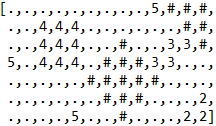
\includegraphics[width=0.45\textwidth]{figures/EC/directEncoding-gen2.png}
     }
     \hfill
     \subfloat[Phenotype\label{subfig-2:directPhen}]{%
       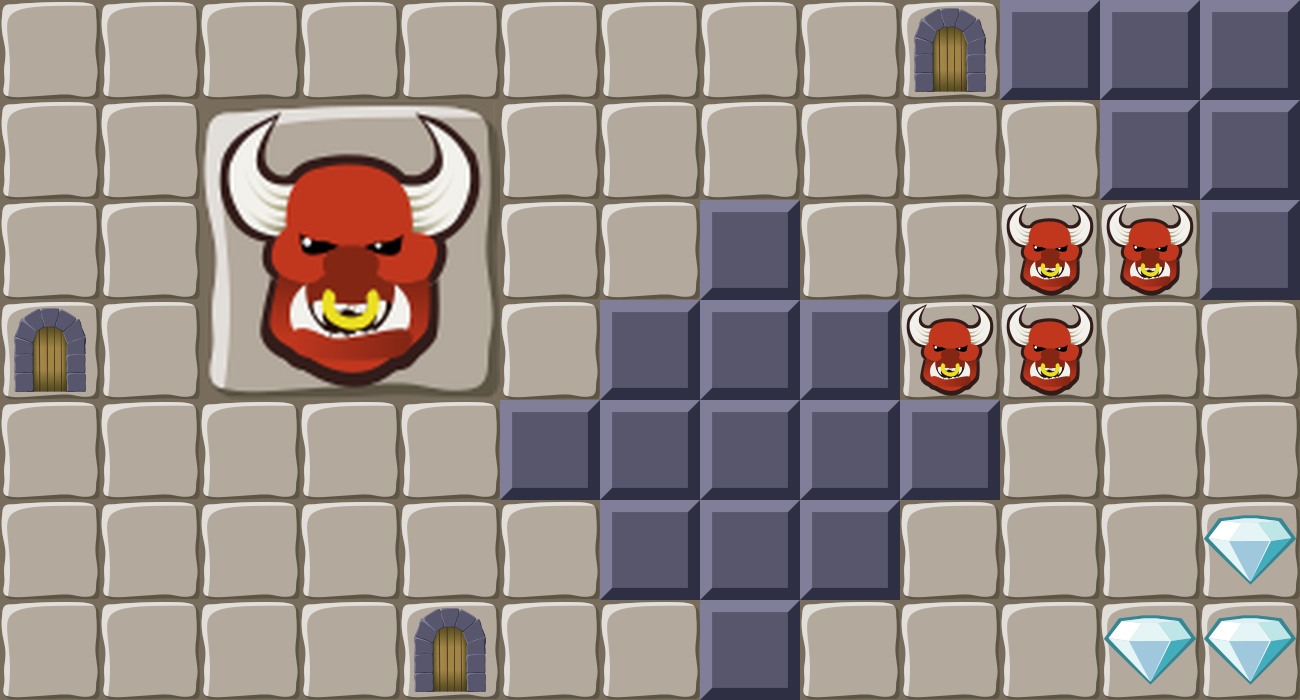
\includegraphics[width=0.45\textwidth]{figures/EC/directEncoding-phen.png}
     }
    
    \caption{Example of direct encoding}
    \label{fig:directENCOD}
\end{figure}

\subsubsection{Evolutionary Algorithm Components}

\paragraph{Representation}
Individuals (i.e., solutions) within a population have two representations: genotypes and phenotypes. \emph{Genotype} is the individual's internal representation within the~\acrshort{ea}, while \emph{Phenotype} is the ``translation'' of the genotype when acting in the environment. For instance, human genotypical representation is the DNA (genotype), while the body, brain, organs, etc. are the phenotypical representation. Such representation and translation are also called \emph{encoding}, which can fluctuate from direct to indirect encoding. 

Direct encoding refers that the genotype is mapped bit-by-bit to the phenotype. In contrast, indirect encoding refers to the opposite, the genotype is minimally encoded, and its representation does not match the phenotype. For instance, in the case of evolving tile-based rooms in a dungeon, a direct encoding could mean that the genotype is an array with integers, each denoting a space in the room and the corresponding tile in the phenotype (shown in figure~\ref{fig:directENCOD}). A lesser direct encoding could have the genotype be an array that groups together areas of the room and marks them as specific areas, or an even lesser let it just be a ruleset (such as in L-systems~\cite{prusinkiewicz_algorithmic_1996,shaker_evolving_2012}) to create the levels. Encoding and representation of individuals are one of the main challenges in~\acrshort{ea} since the encoding can drastically change the evolutionary mechanisms and how the content is generated and explored~\cite{ashlock_representations_2016,clune_performance_2011,stanley_compositional_2007}.

\paragraph{Evaluation}

In an~\acrshort{ea}, it is usually used a fitness function to assess the population and solutions. This estimates the quality of the solutions by testing some metrics that estimate and rank these solutions. Fitness functions are usually context-dependent and help solve the tasks at hand by using some representative heuristic of the task. For instance, if evolving levels in a game, quality can be measured based on the tile distribution or the challenge vs. reward. However, objective-based functions might not be the best way of evaluating content. Environments and tasks could be deceptive with a space filled with local optima, limiting the search; or diversity among the solutions might want to be rewarded rather than just ranking. Stanley and Lehman discuss such challenges with objective-based functions and proposed using divergent searches for stepping stones to solutions, with the aim of open-endedness~\cite{stanley_why_2015}. More work and discussion on this is presented in section~\ref{sec:Backqd}.

\paragraph{Selection}

Selection is used to choose the parents of the next generation of candidate solutions; thus, it chooses which individuals variation operators will be applied to. Selection approaches are biased towards selecting high-quality individuals; after all, these are the ones with the best chances to generate better candidates. However, to counter greedy strategies and avoid getting stuck in local optima, lower-quality individuals still get a chance to be selected (with a similar idea to tabu-search). 
% There are three main approaches to selection: \emph{roulette}: , \emph{tournament}: , and \emph{ranking}:.

\paragraph{Variation Operators}

Once individuals from a population are selected, a set of variation operators are applied to create candidates for the next generation. The operators might be \emph{Mutation} or \emph{recombination} as crossover. Mutation is applied to a single individual with the aims of varying some genes from the genotype to create variation and diversity. For instance, if mutation is not applied, the~\acrshort{ea} is limited to the genes encountered in the initial population; if a key gene was not produced, the global optima might never be found. Common mutation operators are to swap a gene for another in the genotype or randomly change a gene for a random value. Crossover requires at least two individuals that can, as the name indicates, cross their genes to form new candidates. Such is exemplified in figure~\ref{fig:crossoverEX}. The result of applying these operators to the selected parents is a set of candidate solutions (offspring) that are evaluated and compete against the current population for a place in the next generation.

\begin{figure}
\centerline{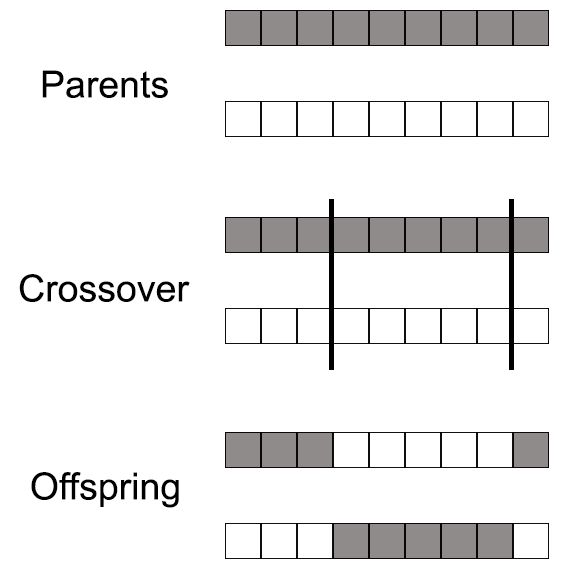
\includegraphics[width=0.5\textwidth]{figures/EC/crossover-example-bw.png}}
\caption{Example of the crossover variation operator
} \label{fig:crossoverEX}
\end{figure}

\paragraph{Replacement}

Replacement strategies mainly focus on replacing lower-quality individuals from the population for better candidates generated through the variation operators, hence, ``survival of the fittest''. However, as it will be explained in section~\ref{sec:map-elites}, not all~\acrshort{ea} work the same. Some have local competition with individuals with similar behavioral novelty~\cite{lehman_evolving_2011}; other approaches have competition among phenotypical similars to preserve innovations encountered in the search space~\cite{stanley_evolving_2002}.

% \begin{algorithm}
% \caption{Evolutionary Algorithm Loop}\label{alg:EA}
% \begin{algorithmic}
% \Procedure{EA}{}
% \State $POPULATION \gets RND\_SOLUTIONS$
% \State $EVALUATE$ each solution \textit{in} $POPULATION$
% % \State $a\gets b$
% % \Procedure{Euclid}{$a,b$}\Comment{The g.c.d. of a and b}
%   \State $r\gets a\bmod b$
%   \While{$r\not=0$}\Comment{We have the answer if r is 0}
%       \State $a\gets b$
%       \State $b\gets r$
%       \State $r\gets a\bmod b$
%   \EndWhile\label{euclidendwhile}
%   \State \textbf{return} $b$\Comment{The gcd is b}
% \EndProcedure
% \end{algorithmic}
% \end{algorithm}

% \subsubsection{Feasible-Infeasible two-Population}

% \begin{itemize}
%     \item What is FI-2Pop
% \end{itemize}

% \subsubsection{Interactive Evolution}

% \begin{itemize}
%     \item simple not extensive text about IE \cite{Takagi2001-InteractiveEvo}
% \end{itemize}

\subsubsection{MAP-Elites} \label{sec:map-elites}

\acrlong{qd} algorithms are a relatively new family of algorithms that leverage the strengths of divergence and convergence search~\cite{pugh_quality_2016}. One algorithm from this family is~\acrshort{mape}, which explores the space yielding a collection of high-performing and diverse solutions. The main characteristics of~\acrshort{mape} are: 1) that it returns a collection of high-performing yet diverse solutions to address multiple wanted behavioral characteristics, for instance, robots that can move around and have a set of different behaviors and characteristics~\cite{cully_robots_2015}. 2) Using behavioral features as dimensions and discretizing the space with cells helps the algorithm illuminate the search space and control niches of solutions. And 3) By using these features and cells, the algorithm is able to substantially explore the space finding in the way a greater amount of solutions than in other approaches.~\acrshort{mape} has been extensively evaluated and resulted in a far superior approach to convergence search (i.e., objective-based) or divergence search (e.g., novelty search) alone, and other~\acrshort{qd} approaches such as~\acrshort{nslc}~\cite{mouret_illuminating_2015}. 

\acrshort{mape}, while superior to other approaches, its iterative cycle is not that different as the one presented earlier in this chapter. The main changes that~\acrshort{mape} introduce are: 1) instead of having one population, the~\acrshort{ea} uses cells; and 2) besides the fitness function to calculate the quality of individuals, it requires a set of behavioral feature dimensions to divide the space into cells and where individuals will be stored. In the vanilla version of~\acrshort{mape}, each cell contains one individual, and as the search encounters new individuals within the same cell, the individual with higher-quality is kept, and the other is disregarded. This way, the algorithm is able to preserve only high-quality solutions while retaining diverse solutions. 

Moreover, the algorithm is shown in Listing~\ref{alg:mape}, which first initializes a collection of individuals evaluated with the fitness function and tested for their behavioral features to be placed in specific cells. Then random selection\footnote{Gravina et al. have experimented on using other selection approaches with beneficial and exciting results~\cite{gravina_blending_2019}} occurs on top of cells to pick individuals that then compete in a classical selection strategy (e.g., comparing fitness) to produce candidate solutions. Variation operators are applied to the selected parents, and the offspring are evaluated with the fitness function and tested for their behavioral features. Depending on the cell the offspring belong, they will need to compete if occupied with the current occupant or if unoccupied, the offspring is placed in the cell, and the cycle restarts. With such a simple algorithm,~\acrshort{mape} can encounter and return a collection of diverse and high-performing individuals. Firstly, this is due to the pressure in cells for high-performing individuals. Secondly, due to retaining individuals in these multidimensional cells, where they might be entirely different for another solution (e.g., have a complete different genotype) yet be as high-performing.


\begin{algorithm}
\begin{algorithmic}
\Procedure{MAP-Elites Algorithm (simple, default version)}{}
\State $(\mathcal{P} \leftarrow \emptyset, \mathcal{X} \leftarrow \emptyset)$
\For{iter $  = 1\to I$}
\If{iter $< G$} 
  \State $\mathbf{x'}\leftarrow $ random\_solution()  
\Else 
  \State $\mathbf{x}\leftarrow $ random\_selection($\mathcal{X}$) 
  \State $\mathbf{x'}\leftarrow $ random\_variation($\mathbf{x}$) 
\EndIf
\State $\mathbf{b'}\leftarrow $feature\_descriptor($\mathbf{x'}$) 
\State $p'\leftarrow $performance($\mathbf{x'}$) 
\If{$\mathcal{P}(\mathbf{b'})= \emptyset$ or $\mathcal{P}(\mathbf{b'})<p'$}
\State $\mathcal{P}(\mathbf{b'})\leftarrow p'$ 
\State $\mathcal{X}(\mathbf{b'})\leftarrow \mathbf{x'}$ 
\EndIf
\EndFor
\State \Return feature-performance map ($\mathcal{P}$ and $\mathcal{X}$)
\EndProcedure
\end{algorithmic}
\caption{Pseudocode description of the MAP-Elites Algorithm. Taken from~\cite{mouret_illuminating_2015}}
\label{alg:mape}
\end{algorithm}

%%UNCOMMENT FOR ADDING THE COMMENTS

% \begin{algorithm}
% \begin{algorithmic}
% \Procedure{MAP-Elites Algorithm (simple, default version)}{}
% \State $(\mathcal{P} \leftarrow \emptyset, \mathcal{X} \leftarrow \emptyset)$\Comment{\emph{Create an empty, $N$-dimensional map of elites:  \{solutions $\mathcal{X}$ and their performances $\mathcal{P}$\} }}
% \For{iter $  = 1\to I$} \Comment{\emph{Repeat for $I$ iterations.}}
% \If{iter $< G$} \Comment{\emph{Initialize by generating $G$ random solutions}}
%   \State $\mathbf{x'}\leftarrow $ random\_solution()  
% \Else \Comment{\emph{All subsequent solutions are generated from elites in the map}}
%   \State $\mathbf{x}\leftarrow $ random\_selection($\mathcal{X}$) \Comment{\emph{Randomly select an elite $x$ from the map $\mathcal{X}$}}
%   \State $\mathbf{x'}\leftarrow $ random\_variation($\mathbf{x}$) \Comment{\emph{Create $x'$, a randomly modified copy of $x$ (via mutation and/or crossover)} }
% \EndIf
% \State $\mathbf{b'}\leftarrow $feature\_descriptor($\mathbf{x'}$) \Comment{\emph{Simulate the candidate solution $x'$ and record its feature descriptor $\mathbf{b'}$}}
% \State $p'\leftarrow $performance($\mathbf{x'}$) \Comment{\emph{Record the performance $p'$ of $x'$}}
% \If{$\mathcal{P}(\mathbf{b'})= \emptyset$ or $\mathcal{P}(\mathbf{b'})<p'$}\Comment{\emph{If the appropriate cell is empty or its occupants's performance is $\leq p'$, then}}
% \State $\mathcal{P}(\mathbf{b'})\leftarrow p'$ \Comment{\emph{store the performance of $x'$ in the map of elites according to its feature descriptor $\mathbf{b'}$}}
% \State $\mathcal{X}(\mathbf{b'})\leftarrow \mathbf{x'}$ \Comment{\emph{store the solution $x'$ in the map of elites according to its feature descriptor $\mathbf{b'}$}}
% \EndIf
% \EndFor
% \State \Return feature-performance map ($\mathcal{P}$ and $\mathcal{X}$)
% \EndProcedure
% \end{algorithmic}
% \caption{Pseudocode description of the MAP-Elites Algorithm. Taken from~\cite{Mouret2015}.}
% \label{alg:mape}
% \end{algorithm}

Furthermore,~\acrshort{mape} have become popular and attractive due to all the abovementioned benefits and characteristics, which have not only spread it's use in many fields and many experiments but also sparked many variations. The Constrained~\acrshort{mape} by Khalifa et al.~\cite{khalifa_talakat_2018} is the one this thesis relies on and has expanded. Their approach added populations in each cell rather than individuals, preserving even more solutions, and combined~\acrshort{mape} with~\acrshort{fi2pop}, which yielded two populations per cell, one driven by the fitness and the other driven by satisfying a set of constraints. Through this, they applied the same process as with the vanilla~\acrshort{mape} but per population (i.e., feasible and infeasible), which resulted in useful and interesting results for the generation of bullet hells bosses.

%%%%%%%%% HERE IS WHERE ICMAPE WAS

% Our fitness function being adaptable

%  this would only focus on obtaining one high-performing individual, 2) the search would focus in fewer places of the generative space, and as a consequence, 3) the diversity of the generated individuals would be scarce. T

% explores the behavioral space for a collection of solutions that are both high-performing and diverse among each other, with the caveat that~\acrshort{mape} discretizes the behavior space as a grid of cells informed by a set of feature dimensions that illuminate the behavior space.

\subsection{Machine Learning}

\acrfull{ml} is a sub-field of~\acrshort{ai} that focuses on using learning algorithms that can learn from data and that are trained through some strategy such as supervised learning or reinforcement learning~\cite{goodfellow_deep_2016}. Formally (and generally), learning in~\acrshort{ml} was operationally defined by Mitchell~\cite{mitchell_machine_1997} as: “A computer program is said to learn from experience \textit{E} with respect to some class of tasks \textit{T} and performance measure \textit{P}, if its performance at tasks in \textit{T}, as measured by P, improves with experience \textit{E}.” 

The task~\textit{T} in~\acrshort{ml} is not the learning \textit{per se}, rather learning is the way to attain the ability to solve the tasks.~\acrshort{ml} helps us solve complex tasks that are deemed too complex to be solver by fixed programs such as the creation of games~\cite{summerville_procedural_2018} or playing games~\cite{mnih_human-level_2015,justesen_deep_2020}. Tasks in~\acrshort{ml} might be a \emph{classification} task: what category \textit{k} an input belongs~\cite{clanuwat_kuronet_2019}; a \emph{regression} task: where it is asked to predict some numerical value based on some input; \emph{synthesis} task: create new examples based on the training samples~\cite{torrado_bootstrapping_2020}; or \emph{machine translation} task: translate an input from one language to another~\cite{hartmann_comparing_2019}.

Moreover, performance~\textit{P} relates to how a learning model is assessed to check that it is learning from experience~\textit{E} to tackle task~\textit{T}. Depending on the type of task that the model must solve, the performance measure would vary, as it is dependant on it, similarly as to how fitness functions are dependant on the problem to be solved. The usual performance measures used are \textbf{accuracy} and \textbf{error rate}. For tasks such as image generation the \textbf{inception score} is normally used~\cite{salimans_improved_2016} or for machine translation the \textbf{BLEU} is used to measure the quality of the translated text~\cite{papineni_bleu_2002}. The key aspect when evaluating performance in a task is that the learning model should be tested with data it has not used for learning, thus showing the ability of the model to solve ''unknown'' tasks~\cite{goodfellow_deep_2016}. 

Furthermore, experience~\textit{E} is related to the data and examples provided to the tool and what strategy is used to train a learning model. Learning strategies in~\acrshort{ml} can be categorized in two main learning strategies: \emph{Supervised} and \emph{Unsupervised} learning. However,~\acrfull{rl} has gained tremendous interest from the research community, and is the current learning strategy that is used to solve many tasks due to the metaphor regarding how human's learn and the fact that the learning happens by experiencing the environment rather than learning the data~\cite{juliani_obstacle_2019}.~\acrfull{ssl} has also been gaining popularity as an approach to move away from traditional supervised training by not using human-annotated dataset to learn representations of data~\cite{doersch_multi-task_2017}.

Within~\acrlong{pcg} and games,~\acrshort{ml} has been increasingly used, gaining popularity to generate different types of content.~\acrshort{pcg} via~\acrshort{ml} is a prospect area that encompasses all algorithms and approaches where the generated content is the output of models trained on existing content~\cite{summerville_procedural_2018}. On the other hand,~\acrshort{ml} can take advantage of~\acrshort{pcg} approaches that continuously create content to increase generality, as discussed by Risi and Togelius~\cite{risi_increasing_2020}. Moreover, Liu et al. discuss the different deep learning approaches used thus far for~\acrshort{pcg}, the open areas for research, and more in detail on the benefit of these approaches both for the deep learning community and the~\acrshort{pcg} community~\cite{liu_deep_2020}.

%or instance, they have the opportunity to be used to increase the generality of~\acrfull{ml} approaches~\cite{Risi2020-pcgGeneralityML},

%%Discuss 
% Over the past years,~\acrshort{ml} has gain popularity in the field of~\acrshort{pcg} in what is called~\acrshort{pcg} via~\acrshort{ml}~\cite{summerville2018procedural}. 
% ~\acrshort{pcg} via~\acrshort{ml} is a prospect area that have shown exciting results for generating a vast amount of game content. Yet creating game levels~\cite{Snodgrass17-GenerateMapsMArkovModels}  for approaches 
% Approaches using supervised learnin
% With datasets such as the Video Game Level Corpus~\cite{Summerville2016-vglc}, many approaches have been 


%%%%%%%%% HERE IS WHERE DESIGNER PREFERENCE AND DESIGNER PERSONAS WAS
%%%%%%% I think perhaps i need to then write about active learning and those things, and sequential mining and clustering approaches.


\section[EVOLUTIONARY DUNGEON DESIGNER]{EVOLUTIONARY DUNGEON \\DESIGNER}
\label{sec:edd}
This section presents the~\acrfull{edd} research tool, all its subsystems and features, and the multiple interactions between the human designer and the computational designer. First, it describes the tool's objectives, the iterations it has gone through, and game design patterns as a significant feature. Then, it presents and discusses the room and narrative generation process, the intertwined attempts, and multiple designer interactions. Finally, it describes the tool's workflow and presents some examples.

% \begin{itemize}
%     \item Total description of EDD, and what it enables
%     \item workflow and development
% \end{itemize}

\begin{figure}[!h]
\centerline{\includegraphics[width=\textwidth]{figures/EDD-figs/map-figure.png}}
\caption{Main level design components in EDD. (a) Basic example room, (b) different placeable tiles (the boss tile looks the same as the enemy tile but 3 times bigger), (c) spatial-patterns and (d) meso-patterns} \label{fig:tilesPats}
\end{figure}

The~\acrshort{edd} is an~\acrshort{micc} system to create adventure and dungeon crawler content, similar to the ones found in Zelda~\cite{tloz} or the Binding of Isaac~\cite{bindingISAAC}. The main feature of~\acrshort{edd} is the collaboration between human and computational designer to create levels and narrative. Within level design, the human designer focuses on editing the room to design their goals while in parallel, they are continuously offered a set of suggestions adapted to their current design. In addition, the designer's design is continuously evaluated for design patterns, feasibility and playability constraints, and enhanced information of the rooms such as door safety or enemy-treasure balance. Within narrative design, the human designer can focus on the creation of quests and overarching narrative structures, while the computational designer collaborates by suggesting quest actions and auto-completing quests, and suggesting diverse narrative structures adapted from the designers structure and level design constraints. Likewise, the computational designer assesses the level design changes that might invalidate quests and change narrative structure constraint.

% the designer is provided with additional information

The first iteration of~\acrshort{edd} was described and presented by Baldwin et al.~\cite{baldwin_mixed-initiative_2017,baldwin_towards_2017}. In their work, the aim was on creating the first steps towards a~\acrshort{micc} system that allowed the designer to create fixed-sized individual rooms while receiving four generated rooms with diverse targets upon request.~\acrshort{edd} was developed further with a revamped UI, allowing the creation of complete dungeons, and providing augmented information on the suggestions compared to the current design~\cite{alvarez_fostering_2018,alvarez_assessing_2018}. The next version of~\acrshort{edd} allows the designer to create dungeons in whatever layout preferred, and incorporates the~\acrlong{icmape}, providing a customizable grid of suggestions steered by the selected feature dimensions~\cite{alvarez_empowering_2019,alvarez_interactive_2020}. Narrative aspects were included in the following iterations. Automatic objective assessment~\cite{flodhag_make_2020} and quest creation and generation~\cite{alvarez_questgram_2021,larsson_queststories_2021} were included in the next iteration. Dungeons were assessed for overarching objective placement, and designers could add different NPCs and quest items in their levels to couple quest actions to them, receiving suggestions from the computational designer. Finally, the last iteration included the creation of overarching narrative structures~\cite{alvarez_tropetwist_2022,alvarez_story_2022}, where designers could set characters, factions, conflicts, objectives, and main or side events, while receiving suggestions in the same line as when creating rooms using the~\acrshort{icmape}. All of the available views where the designer can create content and interact with different parts of the system are shown in figure~\ref{fig:eddWorkflow}. In addition,~\acrshort{edd} now includes prototype implementations of different designer models: the designer preference model~\cite{alvarez_exploring_2020} and designer personas~\cite{alvarez_designer_2022}.

\begin{figure}[t]
\centerline{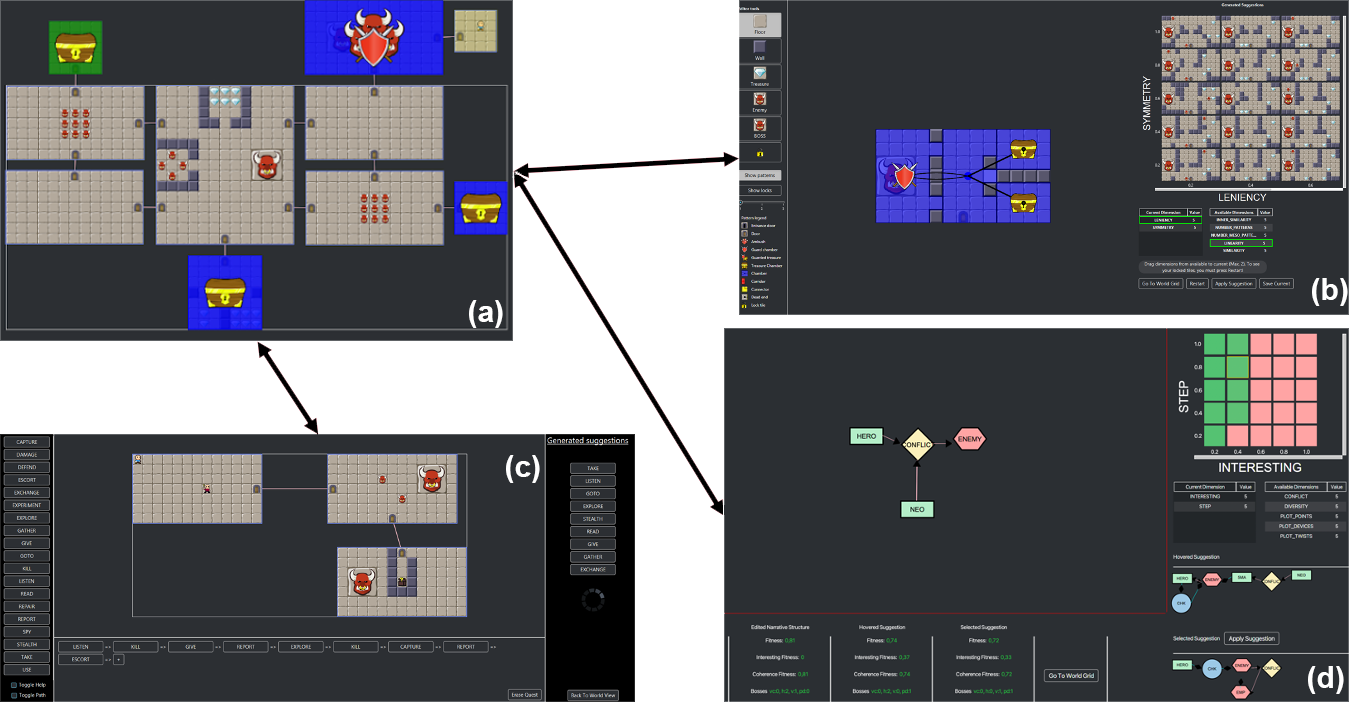
\includegraphics[width=\textwidth]{figures/EDD-figs/eddworkflow.png}}
\caption{Workflow of the~\acrlong{edd}. (a) Shows the world view with a prototype dungeon (\textsc{papers i, ii, iii}) and it's automatically assessed objectives (\textsc{paper vi}). (b) Shows the room view, the main interactive view of~\acrshort{edd}. In this view the designer can edit their room while the computational designer is offering suggestions for their design (\textsc{papers i, ii, iii, v}). (c) Shows the QuestGram view, where designers can use their current dungeon to add different quest actions linked to the room elements (\textsc{paper vii}). Finally, (d) shows the Story Designer view, where designers can create the overarching narrative structure for their game (\textsc{papers x, xi}).} \label{fig:eddWorkflow}
\end{figure}

%Finally, the latest version of~\acrshort{edd} is the one presented on this thesis, which incorporates the~\acrshort{icmape} and allows the designer to create dungeons in whatever layout preferred~\cite{alvarez_empowering_2019,alvarez_interactive_2020}. In addition,~\acrshort{edd} now includes prototype implementations of different designer models: the designer preference model~\cite{alvarez_exploring_2020} and designer personas~\cite{alvarez_designer_2022}.




% ~\acrshort{edd} has four views that enable the~\acrshort{micc} wokflow.

% \subsection{Room Configuration}
\subsection{Level Design}

Dungeons in~\acrshort{edd} are a cyclical graph composed of interconnected rooms. Rooms are a rectangular $M \times N$ grid of tiles, which might be: \emph{Floor}, \emph{Wall}, \emph{Treasure}, \emph{Enemy}, \emph{Enemy Boss}, and \emph{Door} (all shown in figure~\ref{fig:tilesPats}.b). \emph{Wall} tiles are obstacles that cannot be traversed by the player, while all the other are considered passable and could be ``interacted'' by the player. \emph{Enemy boss} tiles are a special type of tile that occupies a $3\times3$ area, as its challenge might be comparable to nine enemies, and only two at a time can co-exist in a room. Doors cannot be placed at will by the designer but might be added when connecting rooms in the world view. 

%\subsubsection{Level Design Patterns}

An essential part of~\acrshort{edd} is its use of level design patterns to hierarchically divide a room into micro-patterns (inventorial and spatial patterns) and their combination into meso-patterns. The level design patterns in~\acrshort{edd} are based on~\cite{bjork_patterns_2004,dahlskog_patterns_2015,dahlskog_procedural_2014}. While~\acrshort{edd} is an~\acrshort{micc} tool to create dungeons for adventure games, we can leverage design patterns to create a generic and domain-independent tool. Through this, we do not need strict definitions or constraints based on specific tiles or functionalities. Rather we rely on patterns that can be made into specific content by the designer if needed.

The design patterns are used in two ways. First, they are used to evaluate the designer's design and show the designer how the system categorizes different parts of the rooms. Second, and more important, design patterns are used to estimate the quality of a generated room. By extracting the patterns of the designer's design and evaluating the generated rooms based on that, design patterns can be used as goals to be achieved by the generated content. In EDD, we have defined \emph{micro-patterns} as the minimum bits that compose the room, and are divided into \emph{inventorial} and \emph{spatial} patterns. \emph{Inventorial patterns} are individual passable tiles, and \emph{spatial patterns}, are a combination of passable tiles and walls resulting in chambers, corridors, and different intersections. 

\emph{Meso-patterns} are the next level in the design pattern hierarchy. They are the composition of micro- and meso-patterns. The meso-patterns that are currently implemented are (shown in figure~\ref{fig:tilesPats}.d): \emph{dead-end}, \emph{ambush}, \emph{guard chamber}, \emph{treasure chamber}, \emph{guarded treasure}.

%To perform this evaluation, design patterns in~\acrshort{edd} calculate a \emph{quality} metric. For instance, the enemy pattern's quality is a combination of the number of enemies placed in the room and how they are distributed. Thus, if the enemies are a certain amount and are not simply added next to each other but distributed with other patterns, the ``enemy quality'' improves.



%the work by Bjork and Holopainen~\cite{bjork_patterns_2004}, Dahlskog et al.~\cite{dahlskog_patterns_2015}, and Dahlskog and Togelius~\cite{dahlskog_procedural_2014}. While~\acrshort{edd} is~\acrshort{micc} tool to create dungeons for adventure games, we can leverage design patterns to create a generic and domain-independent tool. Through this, we do not need strict definitions or constraints based on specific tiles or functionalities. Rather we rely on patterns that can be made into specific content by the designer if needed.

% without strict definitions or constraints based on specific tiles or




% Through this, the system extract the patterns composing the rooms and use it as an estimator of 

% which allows for the comparison of an objective estimation, and to extract possible .

% and through combining these patterns form a new set of patterns. Design patterns are inspired 
% Design patterns 

% \paragraph{Tiles}

% Further, the designer can edit all the rooms with the following set of tiles: \emph{Floor}, \emph{Wall}, \emph{Treasure}, \emph{Enemy}, and \emph{Boss}. When editing their rooms, the designer can activate

% \paragraph{Micro-patterns}

% Micro-patterns are the minimum bits that compose an artifact, in this case, a room. Micro-patterns in~\acrshort{edd} are divided into inventorial patterns and spatial patterns. Inventorial patterns relate to each individual passable tile; thus, each passable tile is represented by an inventorial pattern, and its aggregated quality can be measured. Spatial patterns are composite patterns based on the used space and are a combination of passable and unpassable tiles (i.e., walls).

% Inventorial patterns relate to passable tiles. Yet, rather than calculating each pattern's quality based on individual tiles, they are calculated as a whole. For instance, two enemies placed in different parts of the level will have a shared quality. Inventorial patterns' quality is a trivial calculation based on a user-defined target proportion and the number of tiles of the same type in the room. Doors are a special inventorial pattern, where their quality is based on a linear combination of four measures: \emph{door safety}, \emph{door greed}, \emph{average treasure safety}, and \emph{treasure safety variance}.

% Spatial patterns focus on each room's spatial characteristics and are categorized as a combination of passable tiles and walls. A combination of spatial patterns might give an indication of the type of gameplay the designer wants to create. For instance, multiple interconnected chambers in a room could indicate more small goals within a room and where combat could take place with more maneuvers.

% The spatial patterns are (shown in figure~\ref{fig:tilesPats}.c): \emph{chamber}, \emph{corridor}, \emph{t-junction}, \emph{turn}, and \emph{intersection}. Like inventorial patterns, they are also driven by user-defined targets for creating ``high-quality'' areas and user-defined minimums for areas to be identified as a spatial pattern. For instance, a chamber is identified if there exists at least a $3 \times 3$ open area in a room. Quality is also a trivial calculation based on the expected user-defined targets and the spatial pattern's actual proportion.
% % In figure~\ref{fig:tilesPats}.b, all the possible spatial patterns are shown, and these ar. 

% % Nevertheless, when both inventorial and spatial patterns are used to evaluate generated rooms while the designer works in their design, the user-defined targets are replaced, to a large extent, by the designer's design.
 
% \paragraph{Meso-patterns}

% Meso-patterns are the next level in the design pattern hierarchy. They are identified as pattern compositions and are defined as how micro- and meso-patterns relate. For instance, a chamber (spatial pattern) containing some enemies (inventorial patterns) would result in a ``guarded chamber'' meso-pattern.

% The meso-patterns that are currently implemented are (shown in figure~\ref{fig:tilesPats}.d): \emph{dead-end}, \emph{ambush}, \emph{guard chamber}, \emph{treasure chamber}, \emph{guarded treasure}. \emph{Dead-end} is the only meso-pattern that acts as a pattern modifier rather than a composition of patterns. They are calculated by traversing the pattern graph from all the spatial patterns containing a door to all the other spatial patterns. If any spatial pattern can only be reached by one way, the spatial pattern and all the steps towards it that are not connected to other patterns are classified as dead-ends. For the rest of the meso-patterns, the crucial aspect is that their main component is a chamber (spatial pattern). Thus, these meso-patterns can be seen as a specialization of the chamber. 

% \textbf{Ambush:} Relates to a chamber containing at least one enemy and a door (inventorial pattern). Similar to others, the amount of enemies is also a user-defined minimum. 

% \textbf{Guard chamber}: Relates to a chamber containing at least two enemies (inventorial pattern) and nothing else. Similar to others, the amount of enemies is also a user-defined minimum. 

% \textbf{Treasure chamber:} Relates to a chamber containing at least two treasures (inventorial pattern) and nothing else. Similar to others, the amount of treasures is also a user-defined minimum. 

% \textbf{Guarded treasure}: Relates to a chamber, which is a dead-end, containing at least two treasures (inventorial pattern) and nothing else, but preceded by a guarded chamber. Similar to others, the amount of treasures is also a user-defined minimum. 





% \subsubsection{Macro-patterns}

\subsubsection{Room Generation}

The main feature of~\acrshort{edd} is to suggest variations of the designer's work that are adapted to their design, interesting, and can foster the designer's creativity. Through this, we seek that~\acrshort{edd} ends representing the role of a colleague, as discussed by Lubart~\cite{lubart_how_2005}. The suggestions use the designer's current room configuration as target ratios (e.g., the number of corridors, the number of inventorial patterns, etc.) to provide adaptive suggestions. However, due to the algorithm's nature, the designer is also suggested content that respects these ratios but might use them differently with a different goal.

For instance, if the designer is creating a room with many corridors, such as a labyrinth, they will be provided with suggestions with a similar distribution of corridors, but utilizing the rest of space in different ways, as shown in figure~\ref{fig:corridorExample}.

\acrshort{edd} uses the~\acrshort{icmape} (explained in detail in~\textsc{papers III, V}) to generate and suggest rooms to the designer. Its main features are the use of divergent and convergent searches, the search space division into cells, the use of behavior feature dimensions, the constrained population per cell, and the designer's ability to interact with it. Through this process,~\acrshort{edd} can provide a grid of evolved high-performing suggestions, adapted to the designer's current design, while representing a diverse set of solutions. For instance, in figure~\ref{fig:corridorExample}, it is shown multiple evolutionary runs when using the same design and the set of generated suggestions. It can be observed that the designer is provided with a set of suggestions that retained their expected ratios and design, but diverse enough that the designer can browse many different variations. It can also be observed the effect of the different feature dimensions, as some of them do not match the expected ratios adequately. Thus, producing bigger variations in the solutions to explore the search space. In figure~\ref{fig:interactiveMAPE}, it is presented an overview of the~\acrshort{icmape} steps applied to the level design facet and the multiple areas designers can interact.


\begin{figure}[!h]
    \centering
     \subfloat[Example room]{%
       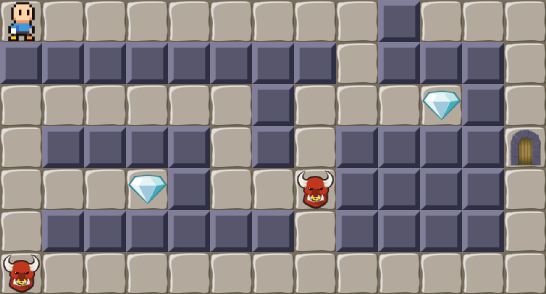
\includegraphics[width=0.48\textwidth]{figures/EDD-figs/corridor_example/currentRoom.png}
     }
     \hfill
     \subfloat[Design Patterns]{%
       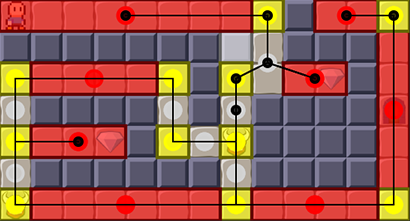
\includegraphics[width=0.48\textwidth]{figures/EDD-figs/corridor_example/room-corridors-final.png}
     }
     
      \subfloat[Meso-pattern and Leniency]{%
       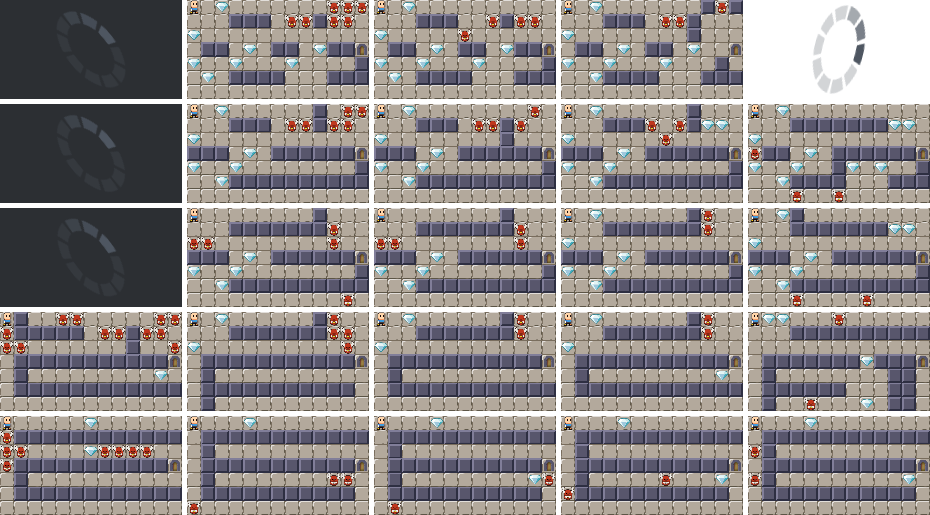
\includegraphics[width=0.48\textwidth]{figures/EDD-figs/corridor_example/meso-leniency-final.png}
     }
     \hfill
     \subfloat[Symmetry and Leniency]{%
       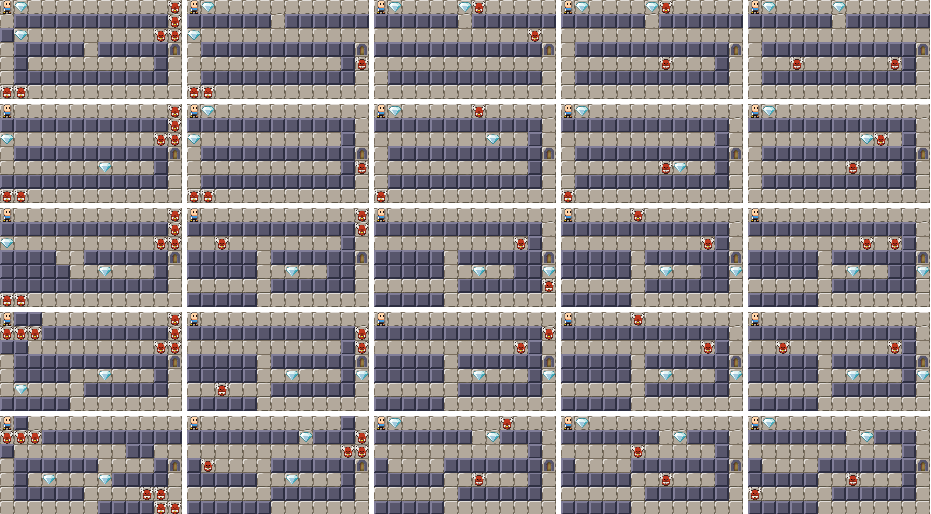
\includegraphics[width=0.48\textwidth]{figures/EDD-figs/corridor_example/sym-leniency-final.png}
     }
    
    \caption{Example of a possible room created by a designer (a), the design patterns identified by the system (b), and two suggestion grids presented to the designer (c and d). The rooms in both suggestion grids, were generated using~\acrshort{icmape} using respectively, \#meso-patterns and leniency (c), and symmetry and leniency (d) as dimensions.}
    \label{fig:corridorExample}
\end{figure}


%\paragraph{Evolutionary Components}

%\acrshort{icmape} is an extension of the Constrained~\acrshort{mape}, which uses a~\acrshort{fi2pop} and~\acrshort{mape} at its core. In our implementation of~\acrshort{icmape}, a solution is deemed infeasible if the playability constraints are not satisfied, i.e., there is a passable tile that is not reachable from at least one door. If this happens, the solution is placed in the respective infeasible population to evolve into a feasible one encouraging diversity in the population.

%Moreover,~\acrshort{edd} implements seven behavior feature dimensions (shown in table~\ref{table:mape-dimensions}). The designer can select one at a time, and only two dimensions can be active at any given time, in order to be able to present the suggestions intuitively to the designer and to focus the search on the pair of dimensions. By giving the designer this interaction, they can effectively reshape the search space of the~\acrshort{icmape}.

%Furthermore, besides using feature dimensions to encounter diverse solutions,~\acrshort{edd} uses a single-objective fitness function to calculate the generated rooms' fitness. The fitness is a weighted sum divided equally between (1) the inventorial aspect of the rooms, which relates to the placement of enemies and treasures in relation to doors and target ratios, and (2) the spatial distribution of the design patterns, which refers to the distribution between corridors and rooms, and the meso-patterns that those encompass. The fitness adapts to the user's current design, automatically informing target ratios and distributions to be achieved by the~\acrshort{ea}.

%The fitness function is shown in Eq.~\ref{fitness_func}. $f_{inventorial}$ is the evaluation of the aggregated and normalized quality of treasures, enemies, and doors (inventorial patterns). Quality refers to positioning, safety, and the relation between inventorial patterns. $f_{spatial}$ refers to the quality and distribution of chambers, i.e. open areas in the room and corridors, and the meso-patterns created within chambers. 

%\begin{equation} 
%\label{fitness_func}
%f_{fitness}(r) = \frac{1}{2}f_{inventorial}(r) \,+ \, \frac{1}{2}f_{spatial}(r)
%\end{equation}


% Cells are first created based on the dimensions selected by the user and proceed to initialize the population based on the user's design, evaluate it and assign each individual to the corresponding cell. Before starting each generation, we check if the dimensions have changed, and if so, recreate the cells and populate them with the previous individuals, and proceed through the evolutionary components. We first select uniformly random which cell to choose parents from, and then we select 5 parents through tournament-selection. Offspring are produced through a two-point uniform crossover operation with a 30\% chance of mutation. Offspring are placed in the correct cell and population after calculating their fitness and dimension's information. Finally, cells eliminate the low-performing individuals that over-cap their maximum capacity. Since interbreeding is not allowed, and can only happen indirectly (i.e. the offspring changing population and then used for breeding in consequent generations), the strategies are repeated for each of the populations.

% This procedure is repeated until the user decides to stop the algorithm. Meanwhile, the EA runs for $n$ generations, and once it reaches the specified limit, it broadcasts the found elites. In order to foster the exploration, we first mutate all the individuals from all the populations and cells (while retaining the previous population), and add them into the same pool together with the current edited room without changes. Finally, we evaluate and assign all the individuals to the correct cells, and cells that are over maximum capacity eliminates low-performing individuals.

% Selection is through competition, 

% That means that with a single run,~\acrshort{icmape} is able to generate a grid of solutions


% aligned to their and are interesting 

% The main feature of~\acrshort{edd} is the computational designer, which main task is to represent the role of a colleague as discussed by Lubart~\cite{LUBART2005-computerPartners}. In order to do this, 

% The formula for calculating the fitness score is the following: 

\subsection{Narrative Design}

Within~\acrshort{edd}, narrative is explored in three individual components: main and secondary objectives based on dungeon's topology and level design patterns (\textsc{paper vi}), quests based on the individual tiles (\textsc{paper vii}), and overarching narrative structure (\textsc{papers x, xi}). These components part from the same idea, using and leveraging patterns and structures to formalize the generation and propose content to the designer. It is important to also highlight that in~\acrshort{edd}, in its current state, these narrative components are subordinate to the level design facet. This means that changes in the rooms and dungeon have effects in the narrative, which the computational designer assess, informs the user of the needed changes, and aids on these changes.

% These narrative components are in relation to the designed dungeon.

%All the narrative components are explored in relation to the designed dungeon. In its current state,~\acrshort{edd} narrative components are effectively subordinate to the level design aspect. This means that changes in the rooms and dungeon have consequences in the narrative, which the computational designer assess, informs the user of the needed changes, and aids on these changes.  

\subsubsection{Automatic Objective Assessment}

Leveraging on the dungeon's structure and the patterns that arise from the designers' design for each level, we calculate possible objectives in the dungeon. The main idea is to utilize the dungeon as much as possible, which means that dead-end rooms without bosses would yield side objectives for players to encourage exploration through side objectives. Likewise, depending on the content within rooms, a room would be selected as the main objective for players, prioritizing boss rooms and rooms farthest from the start position. 

The process is simple and asynchronous from the design tasks, but with significant design impact. It gives insight to designers on what type of objectives are assessed based on the rooms they are designing, and the dungeon's topology. However, these objectives just show the assessment done in EDD, but have no functional use. This means that designers could take this objective assessment, agree with it, change the design to achieve other objectives for players, or disregard the assessment. 

%Then designers could change the design to achieve the objectives they prefer for the players.

\subsubsection{Quest Design}

Narrative was further explored by implementing a quest editor for designers to compose quests within~\acrshort{edd}, called QuestGram (in \textsc{paper vii}). QuestGram provides a new view in EDD for designers to concatenate abstract quest actions connected to individual tiles among all the designed rooms to design quests (a long quest sequence with implicit subquests, which was reformulated as explicit subquests in~\cite{larsson_queststories_2021}). The system also makes use of two new tiles, quest item and quest NPC that certain quest actions can be assigned to. For instance, ``Listen'' can only be associated to quest NPCs, while ``Damage'' can be assigned to several tiles. 

QuestGram is a mixed-initiative system within EDD that complements EDD's original purpose as a mixed-initiative system for level design. The computational designer uses grammars (specifically, L-System) to propose suggestions to the designer based on the quest they have created so far. The grammar, quest actions that are provided to the designer, and the type of NPC are adapted from the work by Doran and Parberry~\cite{doran_prototype_2011}, which analyzed quests in four different MMOs, and extracted their common structure. As the designer adds quest actions and connects them to different tiles, the computational designer continuously generate quests using the grammar, and the ones that match the current quest are used to propose the next possible quest action for the designer. The designer can then either use or disregard this suggestions. They can also request a quest action from the system ad hoc at any position of the quest by simply clickling on it.

QuestGram is coupled to the level design facet since it requires rooms to be designed beforehand for quest actions to be connected to some tangible element. This means that editing the rooms by adding or removing elements affect what quest actions can be added, and can also invalidate parts of the quest in case of tile, doors, or room removal. Once the designer is back at the quest view, they are showed the affected quest actions and can either decide to manually replace, remove, or use the suggestion to readjust their quest. 

%It is based on the system 
%The computational designer 
%the original purpose  level design facet
%, and at the same time, implements 
%How quests are designed within the system. From where does it come, and what are the actions meaning (dont extend)

\subsubsection{Narrative Structure Design}

When creating objectives, stories, and narrative in general, we can consider their design in a different abstraction level. Rather than defining specific objectives, creating quests bit by bit, or coupling these elements to actual in-game elements, we can define narrative structurally, which can describe an experience or story with an abstract representation as argued by Barthes~\cite{barthes_introduction_1966} and Szilas~\cite{szilas_idtension_2003}. We can create structures using a set of generic building blocks that when connected together define narrative structures. This, in turn, define generic aspects of a story, leading to the identification of events, roles, and narrative elements, without the need of defining the plot or how they will take place.

In \textsc{paper x}, we introduced \emph{TropeTwist} as a step towards defining and identifying narrative structures in games. TropeTwist uses tropes extracted from TVTropes~\cite{richmond_tv_2004} as building blocks and patterns, which can compose together structures represented as graphs in TropeTwist. To evaluate and analyze these structures, we defined a set of patterns that can arise from the interconnection of tropes: \emph{micro-patterns}, fundamental narrative units in the system such as conflicts, characters, or plot devices; \emph{meso-patterns}, emerging from the combination of micro-patterns and other meso-patterns, they denote spatial, semanctic, and usability relationships within the narrative graph; and \emph{auxiliary patterns}, used to identify structural gaps in the graph. Patterns are evaluated based on their quality, and in turn, these are used to evaluate the structure as a whole syntactically (i.e., coherence and consistency) and semantically.

TropeTwist was implemented within~\acrshort{edd} as a parallel mixed-initiative system called Story Designer (\textsc{paper xi}). Story Designer lets designers create narrative structures in the form of narrative graphs as seen in fig.~\ref{fig:eddWorkflow}.d, using TropeTwist's building blocks while receiving suggestions adapted to their structures. Suggestions are generated using IC MAP-Elites adapted to generate narrative structures by evolving graph grammars (i.e., adding and removing rules, and changing both their left- and right-hand side part of rules). Thus, the designer can freely create their narrative graph and the computational designer proposes a suggestion grid adapted to their graph, akin to the level design facet. 


%generated by the~\acrshort{icmape}, adapted to generate narrative structures. Narrative structures are encoded as graphs, and IC MAP-Elites evolves graph grammars 

%Within~\acrshort{edd}, we implemented TropeTwist 

% tropes that do not contain meaningful narrative information. 



%The final narrative design system implemented 

%What are narrative struxtures? Express this as narrative graphs. What are the narrative structure patterns, and how are they used within the system.

\begin{figure}[!h]
\centerline{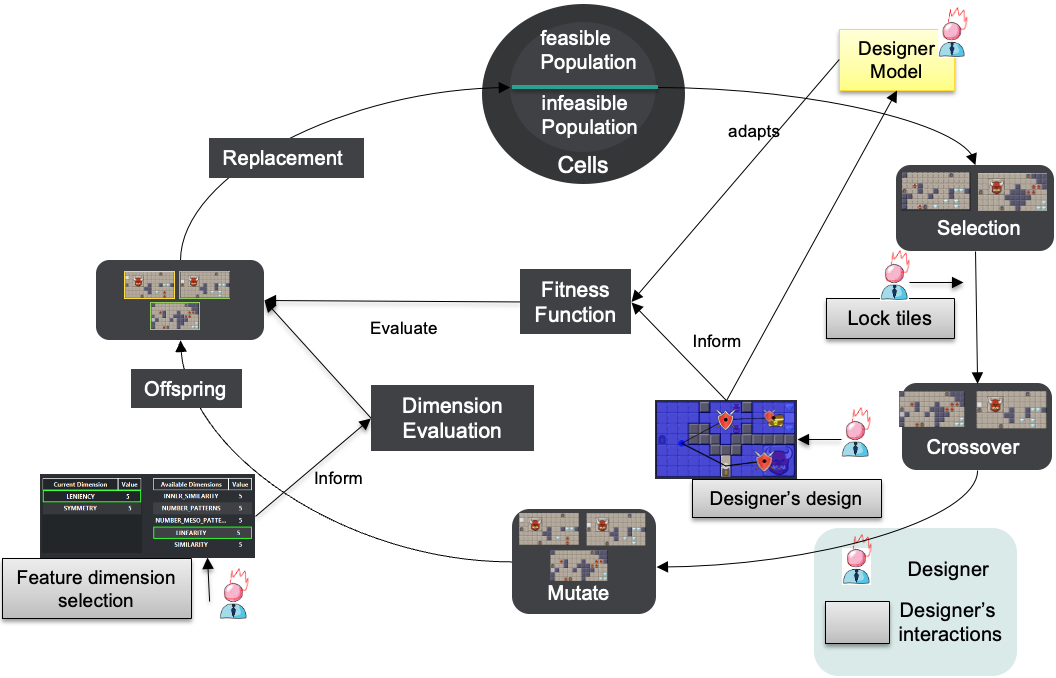
\includegraphics[width=\textwidth]{figures/EDD-figs/all-designers-interactions.png}}
\caption{\acrshort{icmape} evolutionary loop showing the possible designer interactions and what part of the loop these interaction affect} \label{fig:interactiveMAPE}
\end{figure}

\subsection{Designer Interaction}
\label{sec:desInteraction}

A significant feature in~\acrshort{edd}, is the control and interaction designers have with non-intuitive components of the algorithms. In~\acrshort{edd}, the designer always have influence on what the computational designer will create either directly or indirectly. Within the level design facet, the designer can interact with the~\acrshort{icmape} in four different ways: 1) \emph{Locking tiles}: A special tile that locks tiles in the room to be unchangeable (\textsc{paper ii}). 2) \emph{Feature dimensions}: The designer can change the feature dimensions of the~\acrshort{icmape} at any time, reshaping the search space (\textsc{papers iii, v}). 3) \emph{Current design}: The designer is indirectly in constant interaction with the~\acrshort{icmape} by simply designing their room, which adapts the evaluation of generated solutions (\textsc{paper i}). 4) \emph{Designer Model}: As the designer creates their content and uses the suggestions, the system is fed with their interactions, trying to form a model of their preferences (\textsc{paper iv}) and a style and goal model based on their associated designer personas (\textsc{paper ix}).

Within the narrative facet, the designer can interact with it by controlling or influencing the respective algorithm such as the IC MAP-Elites when designing narrative structures or quests, and with the facet itself based on their level design. Concretely, the designer can interact with the algorithms within the facet in two ways: 1) \emph{Developing Quest}: As the designer adds or remove quest actions, the computational designer provides ``next quest action'' suggestions based on the quest up to the selected quest action by the designer (\textsc{paper vii}). 2) \emph{Feature dimensions and narrative structure}: Similar to the level design facet, the designer can interact and change the feature dimensions of the~\acrshort{icmape} when creating narrative structures and at the same time,~\acrshort{icmape} constantly adapts to the designer's narrative structure, leveraging the design as target metric (\textsc{paper xi}). Further, the designer's level design conditions what quest actions will appear and the validity of the quests, what objectives are assessed within the dungeon, and constraints the search space of the~\acrshort{icmape} when generating narrative structures.

% Regarding the indirect control over the narrative facet using the content designed in the level design facet, the designer's design conditions thr


%- Objectives based on their design
% - By adding quest actions, the suggestions take the quest up-to-that point
% - IC MAP-Elites, exactly the same as in level design
% - Their level design conditioning 1) what quest actions will appear and the validity of the quest itself, 2) what objectives are shown, and 3) constraining the search space of IC MAP-Elites when generating narrative structures.

%can interact 


%the designer can interact with the~\acrshort{icmape} in three different ways: 1) \emph{Locking tiles}: A special tile that locks tiles in the room to be unchangeable. 2) \emph{Feature dimensions}: The designer can change the feature dimensions of the~\acrshort{icmape} at any time, reshaping the search space. 3) \emph{Current design}: The designer is indirectly in constant interaction with the~\acrshort{icmape} by simply designing their room, which adapts the evaluation of generated solutions. 

%One of the objectives of this thesis, and a significant feature in~\acrshort{edd}, is the control and interaction designers have with non-intuitive components of the algorithms. In~\acrshort{edd}, the designer can interact with the~\acrshort{icmape} in three different ways: 1) \emph{Locking tiles}: A special tile that locks tiles in the room to be unchangeable. 2) \emph{Feature dimensions}: The designer can change the feature dimensions of the~\acrshort{icmape} at any time, reshaping the search space. 3) \emph{Current design}: The designer is indirectly in constant interaction with the~\acrshort{icmape} by simply designing their room, which adapts the evaluation of generated solutions. 

% The designer can interact with the computational designer, and specifically with the~\acrshort{icmape} that generate the sugthrough

% Besides this, the designer can lock tiles 

% Whenever a designer chooses a suggestion, they are given some extra information 

% \begin{figure}[!h]
% \centerline{\includegraphics[width=0.8\textwidth]{figures/EDD-figs/map-representation-figure-test.png}}
% \caption{Locking Tiles interaction: (a) A sample edited room with (b) its division into zones based on the tiles locked by the user.(c) Suggestions preserve these locked tiles. (d) The room and its zones are internally represented with a tree structure, where the leaf nodes (green) are the valid genes to apply variation operators.} \label{fig:lockTiles}
% \end{figure}

% \textbf{Locking tiles:} Besides the set of tiles provided to the designer to edit the room, they are given a modifier that allows them to lock tiles in their design, which establishes what tiles or structures must be preserved in the suggestions. By locking tiles, the designer is effectively constraining the building blocks~\acrshort{icmape} have for applying variation operators, as mutation and crossover will only happen on non-locked tiles. However, this also allows~\acrshort{icmape} to focus on the areas that the designer is not interested in, segmenting the room's design and promoting the colleague role. Figure~\ref{fig:lockTiles} shows an example of this interaction and how the genes are segmented in the~\acrshort{ea}.

% % the designer is explicitly interacting with~\acrshort{icmape} by establishing what structures must be preserved in the suggestions.

% \textbf{Feature Dimensions:} A major feature in~\acrshort{icmape} that differentiate the approach to other~\acrshort{mape} variations is the interaction designers have with the algorithm. Feature dimensions are an essential component of~\acrshort{mape}, used to discretizes the behavior space as a grid of cells, illuminating such space. Through this,~\acrshort{mape} can explore the space more vastly by retaining high-performing solutions in cells informed by the feature dimensions encountered in different parts of the behavior space. Furthermore, The designer can interact with these feature dimensions, choosing those of most interest to them. By doing this, the search and solutions encountered are conditioned to the designer's interest. Changing the dimensions reshapes the behavior characteristics where encountered individuals in the search space will be retained.

% \textbf{Current Design:}~\acrshort{edd} uses an adaptive fitness function based on the designer's design by analyzing the room configuration based on the design patterns previously described. This allows the designer to interact indirectly with how~\acrshort{icmape} estimates the quality of the encountered solutions. Therefore, to achieve high-fitness, the generated content will need to have certain similar characteristics than the current design, in order for the content to do not be too disparate from the designer's goal. However, while this might limit the tool's expressivity,~\acrshort{icmape} use of feature dimensions and leverage on convergent and divergent searches still yields diverse solutions.

% Finally, in figure~\ref{fig:interactiveMAPE}, it is presented an overview of the~\acrshort{icmape} steps applied to the level design facet and the multiple areas designers can interact.


% \subsubsection{Designer Modeling}

%\subsection{Workflow}

%\acrshort{edd} has three views that enable the~\acrshort{micc} wokflow depicted in figure~\ref{fig:eddWorkflow}.

%\subsubsection{World View}

%In figure~\ref{fig:eddWorkflow}(a), it is shown the world view. This view provides the designer with an overview of their dungeon while allowing them to create new rooms and edit their connections. The dungeon is a cyclical graph in code, which allows the needed flexibility for the designer to create whatever layout they want. The designer can create or delete any number of rooms and can connect them as needed. By editing these connections, they edit the rooms' entrance and exit doors, effectively changing the layout and gameplay flow. For instance, the designer can create linear gameplay with rooms one after the other, or gameplay that rewards exploration through dead-ends with some side-objective. 

%To edit a room, the designer can: 1) double-click or scroll to zoom-in any room to change the view to the \emph{room view} or 2) select a room and click the ``Suggestions'' button, which will take them to the \emph{suggestion view}

%\subsubsection{Suggestion View}

%In this view (shown in figure~\ref{fig:eddWorkflow}(b)), the designer is proposed six variations to their design based on six different preset room configuration: Favoring open areas, favoring corridors, a mix of open areas and corridors, favoring dead-ends, favoring meso-patterns, and using the actual room configuration. The designer can then go back to the world view or choose any of the suggestions and start editing their room using that as a base in the \emph{room view}.

%\subsubsection{Room View}

%The room view (shown in figure~\ref{fig:eddWorkflow}(c)) is the main view in~\acrshort{edd}, where both the designer and the computational designer interact to co-create rooms. As mentioned above, the designer has five different tiles at their disposal to create a room that fulfills their objective. Besides this, the designer can enable the ``patterns visualization'' that overlays on the designer's design what spatial- and meso-patterns are identified.

%\acrshort{edd} incorporates a feasibility and playability check on the designer's design. This informs the designer if an area in the room is inaccessible from within the room or through another room by adding a red border in their design and an information box. This feasibility check is reused in the~\acrshort{ea} used by the computational designer to generate suggestions for the designer. 

%Moreover, in this view, the designer edits the room as they want, while on the right side of the view, they are suggested a collection of rooms. Whenever a suggestion is selected, a quantitative comparison between the suggestion and the current design is presented to the designer. If the designer decides to replace their design with the suggestion, they apply it and continue the design process. The system aims to give suggestions to the designer that are interesting for them, aligned with their current design, but at the same time different enough to foster their creativity. Designers might not apply any suggestion, but a designer might be interested in doing something similar by observing them. 

%Once the designer finishes editing their room, they can go back to the world view and start another room's design process until they finish their dungeon. 

%\subsubsection{Room Objectives}


%\subsubsection{Quest View}

%\subsubsection{Narrative Structure View}









% These rooms can be examined


% when their design do not fulfill the requirements. These are: 1) there is an area in the room that is inaccessible from within the room or through another room

% As the designer creates their room, the system is constantly 




% In~\acrshort{edd} the designer can create individuals rooms of different sizes and interconnect them to compose dungeons with different types of gameplay. 


%\section{ALGORITHMS}  \normalfont

\subsection{Interactive Constrained MAP-Elites}
\label{sec:icmap-elites}

The~\acrfull{icmape}~\cite{alvarez2019empowering,Alvarez2020-ICMAPE} is the main algorithm developed in this thesis, which focuses on adapting the Constrained~\acrshort{mape} to be used in an~\acrshort{micc} system allowing designers to interact with it, and change non-intuitive aspects of~\acrshort{mape}. The main novel characteristics of~\acrshort{icmape} are:
% to be interacted by the designer. 

\begin{itemize}
    % \item Adapting~\acrshort{mape} to be used to co-design levels by proposing suggestions in an~\acrshort{micc} system.
    \item \acrshort{mape} adapted to be used in a~\acrshort{micc} system to collaborate and interact with the designer.
    \item Use of~\acrshort{mape} to create dungeons and adventure levels.
    \item Continuously adapting the fitness landscape and search space based on the designer's creation, which in turn, makes~\acrshort{mape} continuously adapting to a changing space.
    \item Customizable behavioral feature dimensions as part of the designer's ability to interact with the system. By changing the feature dimensions, pressure is imposed in the algorithm to adapt the search as the behavior dimensions are no longer the same (i.e., the niches changed).
\end{itemize}

In terms of the~\acrshort{ea} components, our implementation of~\acrshort{icmape} in~\acrshort{edd} uses direct encoding similar to the one depicted in figure~\ref{fig:directENCOD}, selection is through competition of individuals in each cell population, and selected individuals are applied crossover and mutation. Finally, the replacement strategy is elitist; if any offspring is better than individuals in their cell, these are replaced. 

Moreover, there are three ways designers can interact with~\acrshort{icmape}: 1) By editing their design, which automatically updates and adapt the fitness function. 2) By changing behavior feature dimensions and the size of cells, which is reflected in the algorithm's search space. And 3) By locking areas of their design to be preserved in the evolutionary run, which limits the building blocks~\acrshort{icmape} has to apply variation operators to, but preserves the designer's structures. This last interaction was developed earlier than~\acrshort{icmape} but is still available for the designer, is documented in~\cite{Alvarez2018a}, and presented in section~\ref{sec:desInteraction}.

\begin{algorithm}
%\algsetup{linenosize=\tiny}
\footnotesize
\caption{Interactive Constrained MAP-Elites}\label{alg:ICMAPE}
\begin{algorithmic}[1]
\Procedure{IC MAP-Elites($\protect[\{d_1,v_1\},...,\{d_n,v_n\}]$)}{}
\State $target \gets curEditRoom$ \Comment{Always in background}
\State createCells$(\protect[\{d_1,v_1\},...,\{d_n,v_n\}])$
\For{$i \gets 1$ to $PopSize$} %\Comment{$PopSize \gets 1000$}
     \State add mutate$(target)$ to $population$
\EndFor
\State CheckAndAssignToCell$(population)$ 
\While {true} \Comment{start continouous evo}
    \For{$generation \gets 1$ to $publishGen$}
        \If {$\textit{dimensionsChanged}$}
            \State $previousPop \gets cells_{pop}$
            \State createCells$(newDimensions)$
            \State checkAndAssignToCell$(previousPop)$ 
        \EndIf
        \MRepeat{ \text{[for feasible \& infeasible pop.]}}
            \For{$i \gets 1$ to $ParentIteration$}
                \State $curCell \gets \text{rndCell}(cells)$
                \State add tournament$(curCell)$ to $parent$
            \EndFor
            \State $offspring \gets  \text{crossover}(Parent)$
            \State checkAndAssignToCell$(offspring)$
        \EndRepeat
        \State sortAndTrim$(cells)$
    \EndFor
    \State broadcastElites() \Comment{render elites}
    \State $pop' \gets cells_{population}$
    \State add mutate$(cells_{pop})$ to $pop'$
    \State add $target$ to $pop'$
    \State checkAndAssignToCell $(pop')$
    \State sortAndTrim$(cells)$
\EndWhile
\EndProcedure
\Procedure{createCells(dimensions)}{}
    \ForEach{$dim \in dimensions $}
        \State add newCell$(dim_d, dim_v)$ to $cells$
    \EndFor
\EndProcedure
\Procedure{$\protect \text{check\&AssignToCell}(curPopulation)$}{}
    \ForEach{$individual \in curPopulation $}
        \State $individual_f \gets evaluate(individual)$ 
        \State $individual_d \gets dim(individual)$
        \State add $individual$ to $cell_{pop}(individual_d)$
    \EndFor
\EndProcedure
\end{algorithmic}
\end{algorithm}

In terms of execution,~\acrshort{icmape} is very similar to the vanilla~\acrshort{mape} and Constrained~\acrshort{mape} with three main differences: 1) The evolutionary run never ends and continuously update and adapts the fitness function based on the designer's current design, and through this, populations within cells might change their order, putting new pressure in individuals. 2) After $n$ amount of generations, the designer is presented a collection of suggestions in the same~\acrshort{mape} grid used in the search. When this happens, all individuals in all cells are selected, cloned, and minimally mutated to promote diversity. 3) At any moment, the designer might decide to replace their design with a suggested one, which in turn drastically change the algorithm, since rather than adapting the fitness gradually, the change might directly make high-performing individuals low-performing. However, one of the benefits of~\acrshort{mape} is it's fast convergence; thus, the algorithm adapts fast to the changes. And 4) the designer can change the feature dimensions (a pair at a time) and the amounts of cells per dimension to create bigger or smaller niches. Through this, the designer is effectively reshaping the behavior characteristics where encountered individuals in the search space will be retained, thus changing non-intuitive parameters in intuitive ways. The algorithm is depicted in listing~\ref{alg:ICMAPE}, and some examples of the~\acrshort{mape} grid presented to the designer are shown in figure~\ref{fig:MAPEGrid1}.

\begin{figure}[!h]
    \centering
     \subfloat[]{%
       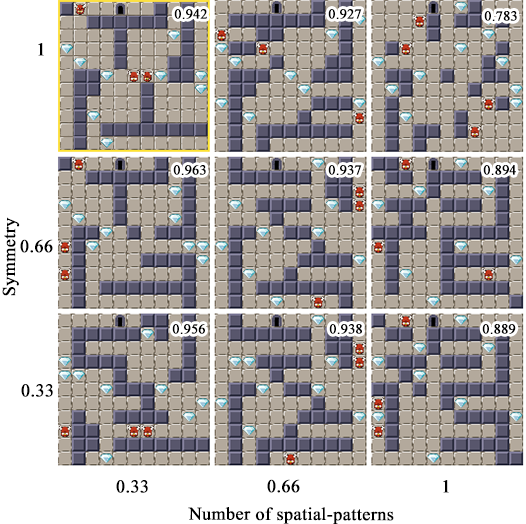
\includegraphics[width=0.49\textwidth]{figures/ICMAPE-figs/figure5.png}
     }
     \hfill
     \subfloat[]{%
       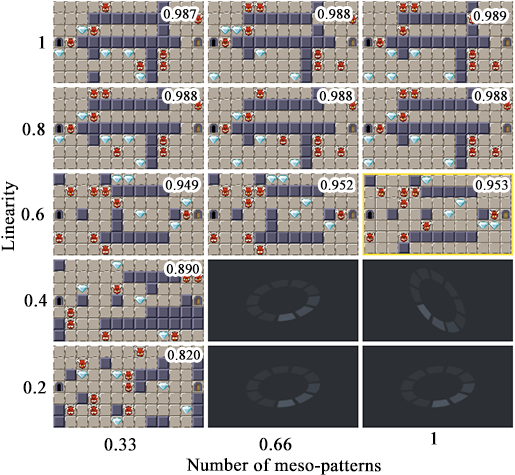
\includegraphics[width=0.49\textwidth]{figures/ICMAPE-figs/figure8.png}
     }
    
    \caption{Examples of suggestion grids presented to the designer as they design different rooms.}
    \label{fig:MAPEGrid1}
\end{figure}

As highlighted, behavioral feature dimensions are one of the main components of~\acrshort{mape} and all of its variations. They are context-dependent similar to fitness functions, with the caveat that they are only used to categorize and place individuals in cells. The features currently available in our implementation of~\acrshort{icmape} in~\acrshort{edd} are presented in table~\ref{table:mape-dimensions} along with a description of each dimension, and an example of each dimension and multiple cells in each dimension is shown in figure~\ref{fig:dimension-examples}. 
% While they are all related to the context of a dungeon and adventure games, there are two dimensions, \emph{similarity} and \emph{inner similarity}, which adapts dynamically to the current, i.e., at different time-steps, it will yield

\begin{table}[ht]
\centering
\caption{Developed game based features used as dimensions in the~\acrlong{icmape}}\label{table:mape-dimensions}
% \resizebox{\textwidth}
% \resizebox{\textwidth}
\begin{tabularx}{\textwidth}{|c|X|}
\hline
\rule{0pt}{12pt}
Feature&Definition\\ \hline
% \\[-6pt]
Similarity & Refers to the aesthetic (tile-by-tile) similarity between a room and the current designer's design.\\ \hline
Inner Similarity & Refers to the similarity of the sparsity and density of the different tile types of a room designer's current design.\\ \hline
Symmetry & Refers to the aesthetic symmetry of a room.\\ \hline
Leniency & Refers to how challenging rooms are; calculated based on the position of enemies and balance between enemies and treasures.\\ \hline
Linearity & Refers to the amount of paths connecting doors within a room; calculated based on how many spatial patterns are traversed.\\ \hline
\#Meso-Patterns & Refers to the number of meso-patterns that exist within a room, normalized by an estimated maximum number based on the room's size and the minimum chamber size.\\ \hline
\#Spatial-Patterns & Refers to the number of spatial-patterns that exist within a room, which can be chambers, corridor, turns, junctions, and intersections.\\ \hline
\end{tabularx}
\end{table}


Finally, Mouret and Clune discuss that a traditional single-objective approach could reach as good fitness in an individual for some of the tasks they experimented~\cite{Mouret2015}. Nevertheless, 1) this would only focus on obtaining one high-performing individual, 2) the search would focus in fewer places of the generative space, and as a consequence, and 3) the diversity of the generated individuals would be scarce. The nature of our mixed-initiative tool not only requires but promotes the identification of multiple solutions that would satisfy similar constraints. For instance, a linear room could be one with narrow corridors connecting doors or a simple open chamber containing all doors. Therefore, a rich, diverse, and high-performing set of levels to be suggested to the designer that could be generated in a short period, and that can adapt to changes over time is a key necessity for~\acrshort{edd}. 
% This motivated the development of~\acrshort{icmape} and is  and essential feature of~\acrshort{icmape}, the motivation for developing~\acrshort{icmape}.

\begin{figure}[!ht]
\centerline{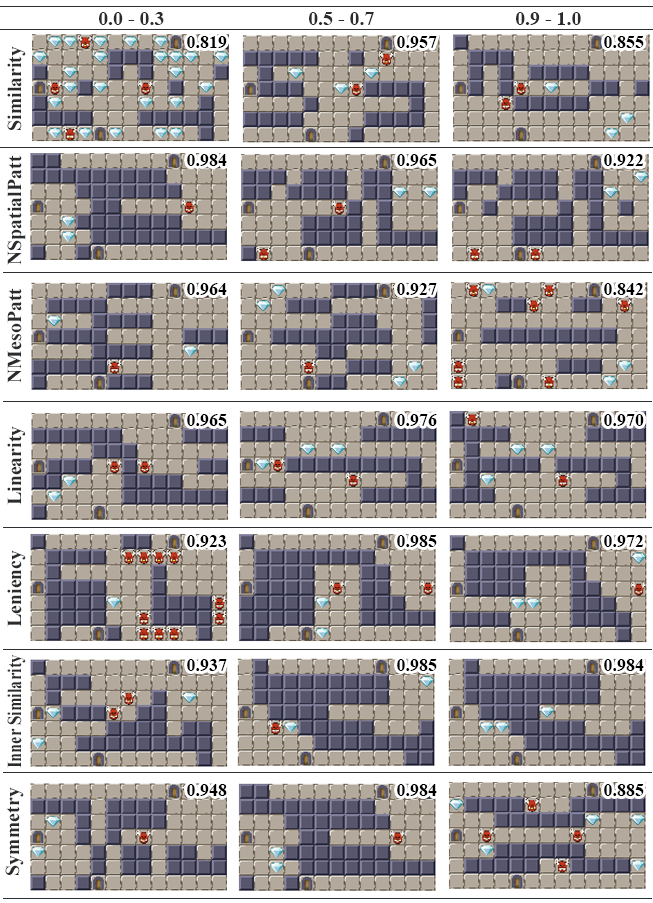
\includegraphics[width=0.7\textwidth]{figures/ICMAPE-figs/figure-all-dimensions-final.png}}
\caption{Example of Elites generated using IC MAP-Elites. Each row represents an independent run of the algorithm using the dimension specified to the left. Each column splits the dimension score into three intervals: 0.0-0.3 (low), 0.5-0.7 (medium), and 0.9-1.0 (high). Each cell displays (top-right) the fitness of the optimal individual in its related interval} \label{fig:dimension-examples}
\end{figure}

\subsection{Designer Preference}

To explore designer modeling and its benefits, the designer's preference model was proposed to drive the content generation in~\acrshort{icmape}~\cite{Alvarez2020-DesignerPreference}. In this work, the suggested~\acrshort{mape} grid is used to compose a dataset used as an estimator of the designer's preferences. The goal and motivation of modeling the designer's preferences were to use a surrogate model that could capture the designer's subjective evaluation and an objective evaluation from the fitness function. The model, the training, and the usage is depicted in figure~\ref{fig:desPrefModel}. 

\begin{figure}
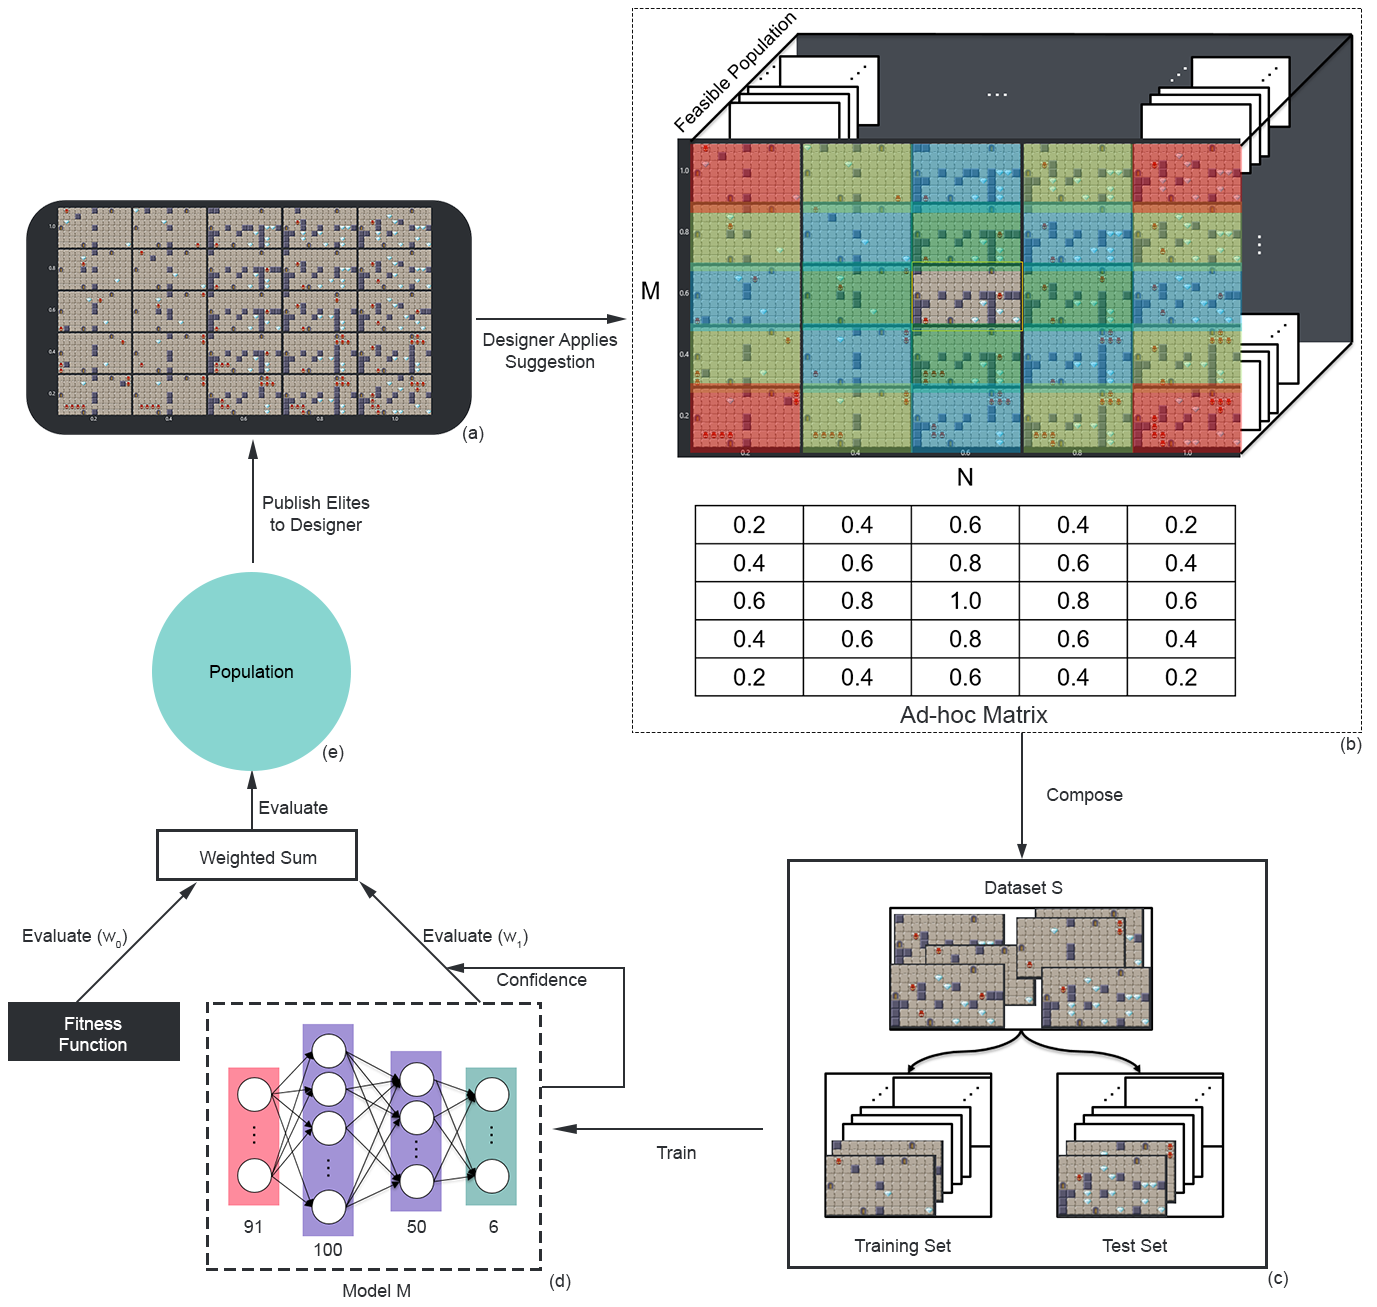
\includegraphics[width=\textwidth]{figures/DesPref-figs/desPrefModel.png}
\caption{Overview of the Designer Preference Model integrated into the fitness function of EDD. Elites are published and shown to the designer in a grid fashion (a). Once the designer chooses and applies one of the suggestions, an ad-hoc matrix is created based on the selected suggestion's position to estimate the preference of suggestions (b). The ad-hoc matrix is then applied to all the elites in the grid and the feasible populations within the EA cells to compose a general dataset $S$ with rooms labeled by the estimated preference. The composed dataset $S$ is then subdivided into a training set (90\%) and test set (10\%), both with the same label distribution (c). The dataset is used to train a model $M$, which is a relatively small neural network for 20 epochs (d). The model is then used to evaluate the population of the EA together with the current fitness function in a weighted sum. The weight of the model $M$ conditioned by the confidence of the network (e).} \label{fig:desPrefModel}
\end{figure}

Following a proactive learning approach~\cite{donmez2008proactive}, whenever the designer chooses some suggestion, the system trained a learning model $M$ (i.e., a neural network) with a new set of preferred content (dataset $S$) using the current suggested cells and their population. The result was an adapted model similar to the work by Liapis et al.~\cite{Liapis2012-adaptiveVisual}, which learned overtime the designer's preferences in relation to their choices. Once the model is trained, it is incorporated in the evolutionary loop to drive evolution by means of evaluating the content in a weighted sum with the fitness function. The model slowly fits towards the designer’s preference, and as it's predictions become more confident, the more weight $W_{1}$ it has in the final evaluation. Confidence is calculated based on the softmax layer's output, which can be interpreted as probabilities for each class. The evaluation resulted in the weights (Eq.~\ref{eq:weights}) and the final weighted sum (Eq.~\ref{eq:weightedSum}).

\begin{equation} \label{eq:weights}
\begin{split}
 w_{1}={}&\min(M_{conf} \cdot M_{TestAcc}, 0.5),\\
w_{0} ={}& 1.0 - w_{1}   
\end{split}
\end{equation}

\begin{equation} \label{eq:weightedSum}
weightedSum = (w_{0} \cdot objective) + (w_{1} \cdot predicted_{pref})
\end{equation}

We evaluated the model and its usability in a user study with fifteen game design students. While not significant as there was not enough data to demonstrate the advantage of the model, the results allowed the analysis of the system's challenges. These challenges were presented as three open areas for active research: \textit{Dataset}: the type and amount of data collected; \textit{Preference modality}: what represents preference in the design and creative process; and \textit{Dynamic-Dynamic System vs. Dynamic-Static System}: the competing properties of a dynamic learning environment, e.g., a designer that traverse the design space, with a dynamically adapting model, e.g., a learning model that tries to adapt as the designer traverse the design space, and it's trade-offs.

\subsection{Style Clustering and Designer Personas}

\begin{figure}
\centerline{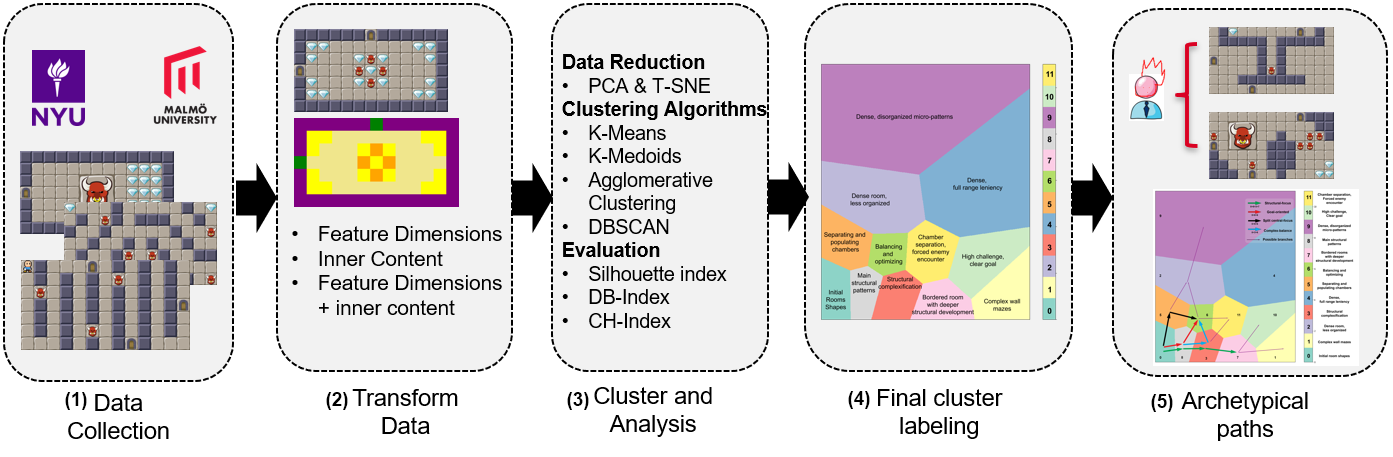
\includegraphics[width=\textwidth]{figures/DesPersonas-figs/process-steps.png}}
\caption{The stages of the design style clustering development: (1) Data was first collected through two user studies. (2) Then, using the design sequences, the data was processed into five different datasets, one using the room images, a second using the tiles information, and three using tabular information. (3) A data reduction technique was applied to different datasets, and then they were clustered and internally evaluated. (4) The clusters were formed, picked from the best-performing methods, and labeled based on the data points within each cluster. The clusters were evaluated by visualizing how a typical design session traverse the various clusters, and K-Means (K=12) was chosen as the final approach. (5) Finally, using this final approach, all the sequences were clustered, and archetypical paths were identified.
} \label{fig:clusteringApproach}
\end{figure}

To further explore designer modeling, an alternative approach was proposed by clustering designers' design styles~\cite{alvarez2020-designerpersonas}. The basic premise was that by identifying a set of styles that most designers follow when creating content, and model how the designer traverse such a style space, a model that captured the designer's intentions, goals, and style could be created. For instance, rooms for a game like the binding of Isaac~\cite{bindingISAAC} could be classified based on multiple characteristics such as the room's objectives regarding enemies and treasures, access to different areas, or hidden challenges and treasures. Moreover, different designers could reach the same room style through different paths, where the focus along the creation could vary. Some designers would focus on the room's topology before anything else, whereas others would focus first on the objectives a player must achieve. 

\begin{figure}[t]
\centerline{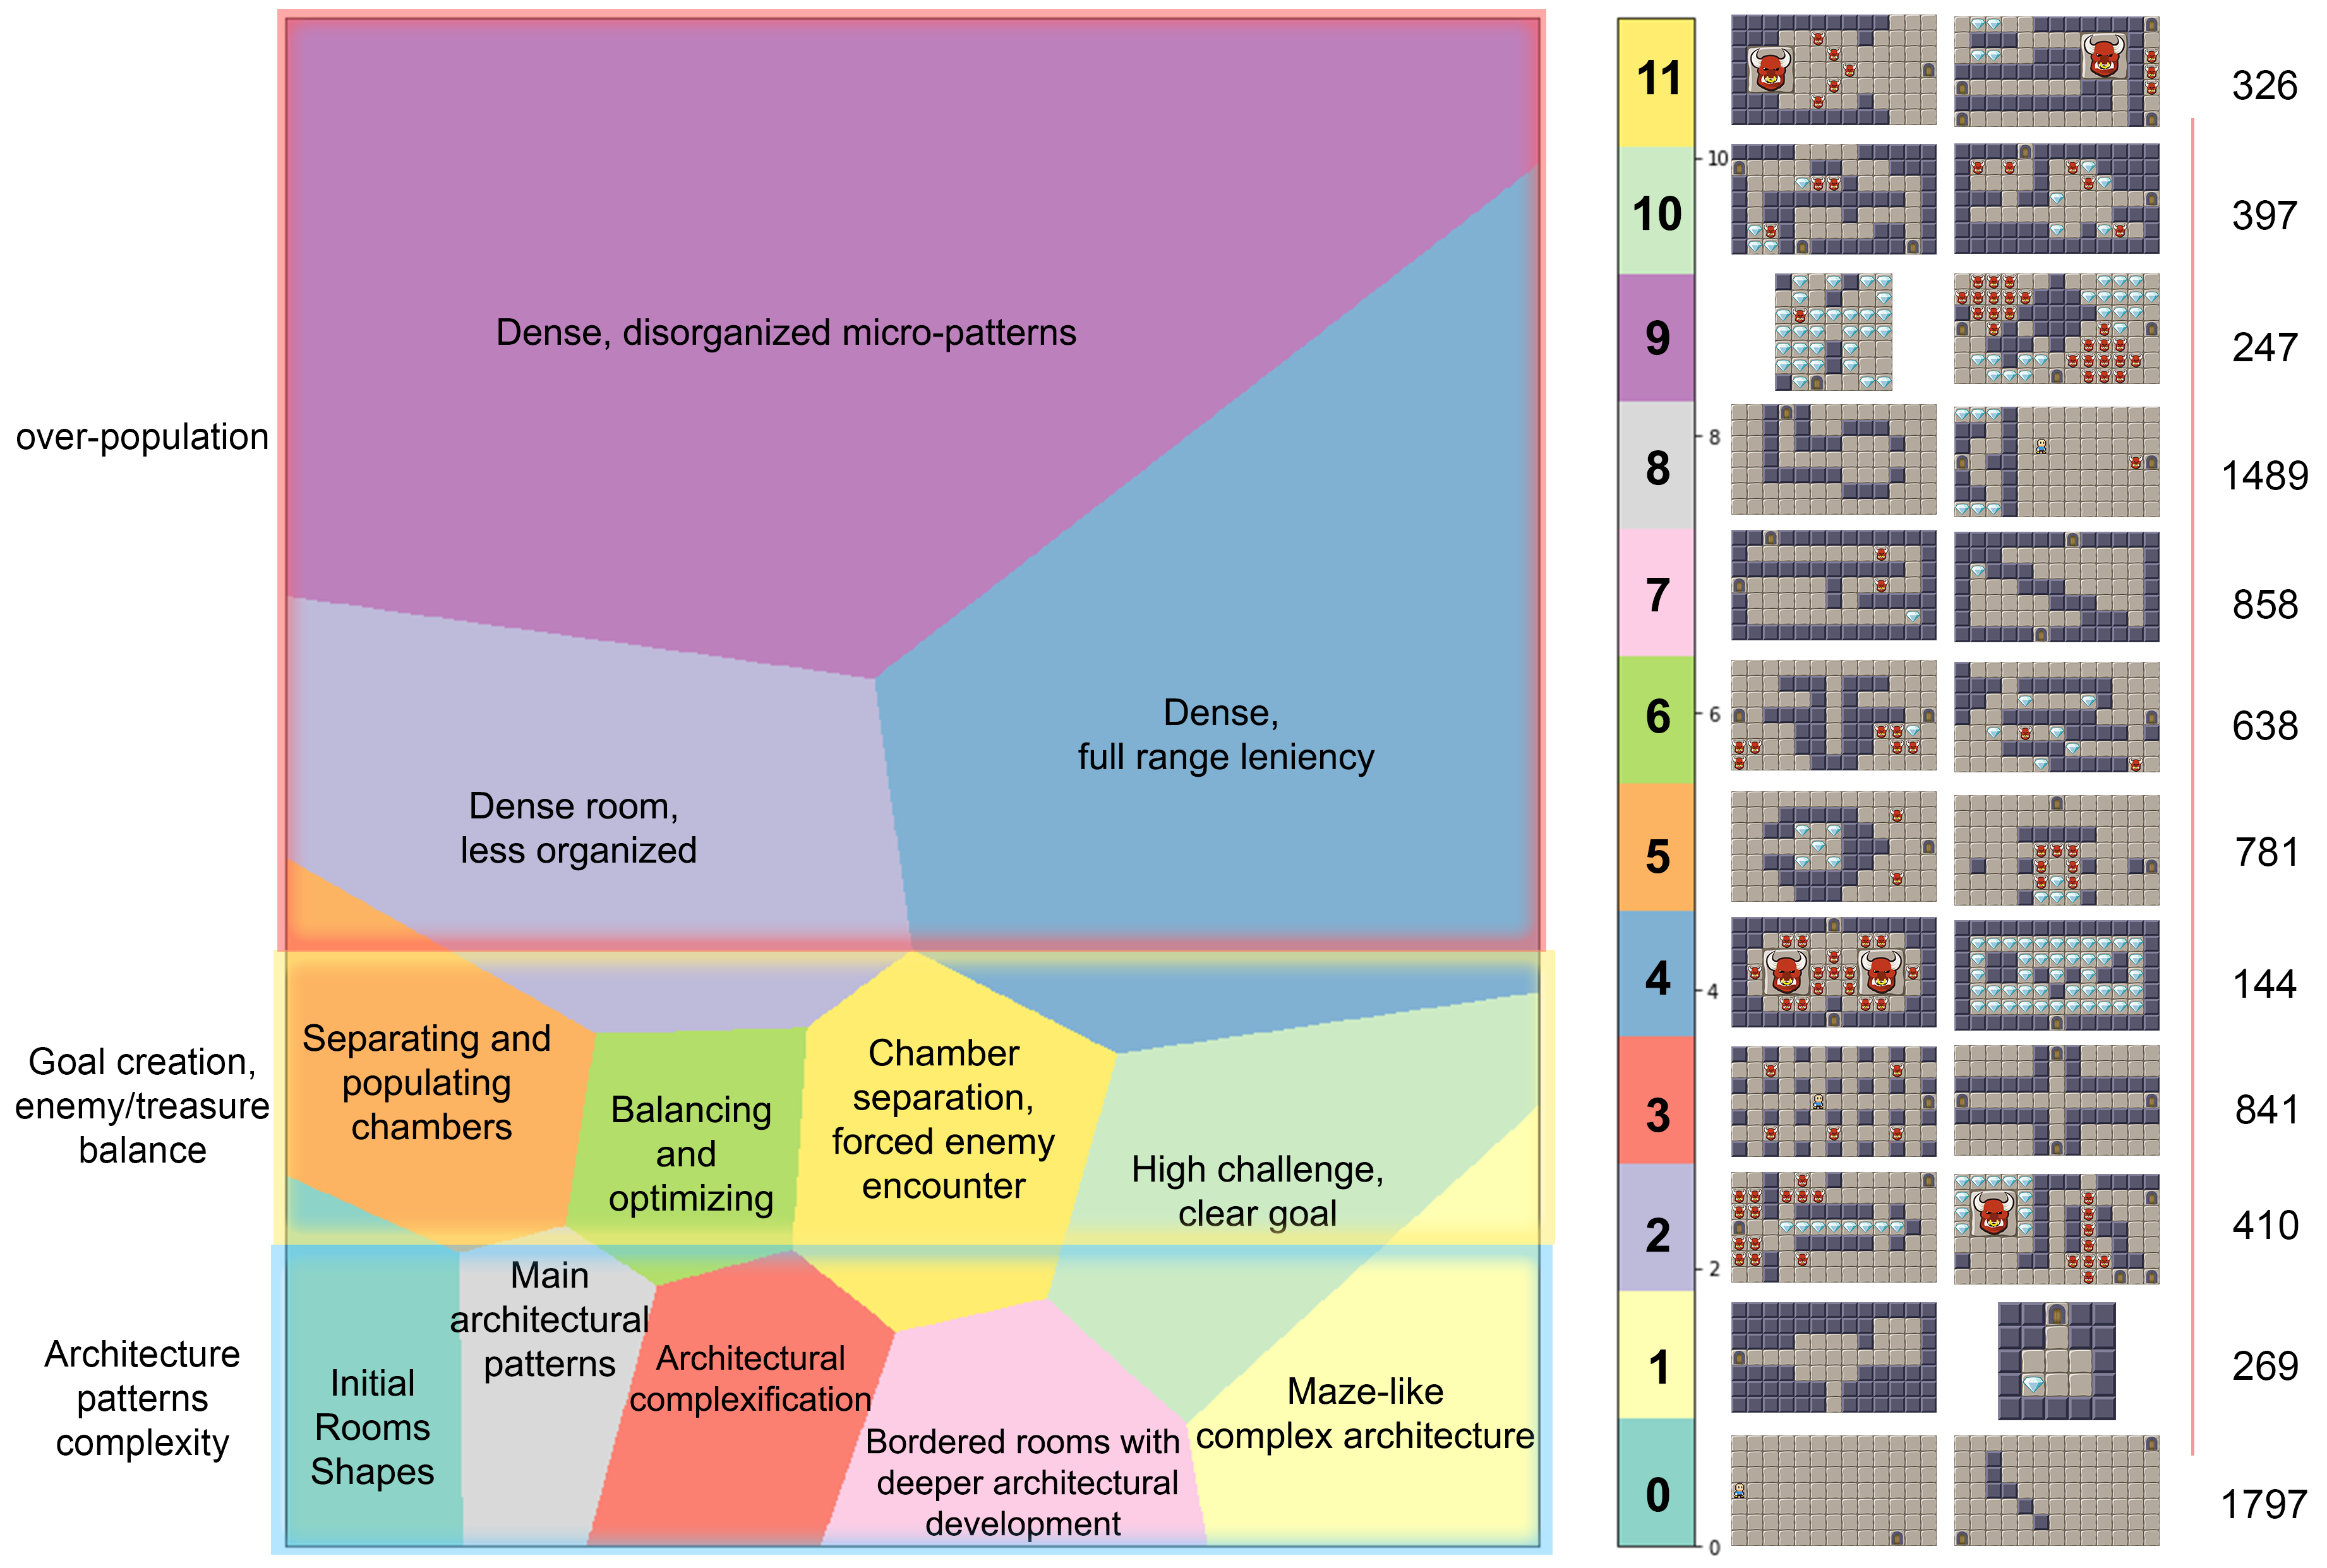
\includegraphics[width=\textwidth]{figures/DesPersonas-figs/final-cluster.png}}
\caption{Best resulting cluster set. K-Means (K=12), using the \textbf{Tiles} Dataset. While it scores slightly less in the internal indices that other setups, a qualitative analysis successfully gives us more granularity by subdividing the main bottom clusters to label and cluster designers' design process. Sample rooms belonging to each cluster are displayed on the right, next to the total number of rooms in the cluster.} \label{fig:all-clusters}
\end{figure}

With such as motivation and objective, it was compiled data of designers' designs and their creation process in the~\acrshort{edd} to create these models. The data was collected from two user studies, the one documented in the Designer's Preference Model previously described~\cite{Alvarez2020-DesignerPreference} with game design students, and another with practitioners and academic researchers within the computational intelligence in games area. The data was used to create five different datasets that were used in the experiment to analyze multiple variations and possibilities. The datasets were analyzed, experimented on, and compared to obtain the final clusters that effectively divided the design style space. The process is shown in figure~\ref{fig:clusteringApproach}. Figure \ref{fig:all-clusters} shows the final design style clusters with the setup that performed best among all the different experiments (K-Means (K=12), using the \textbf{Tiles} Dataset).

\begin{figure}[t!]
\centerline{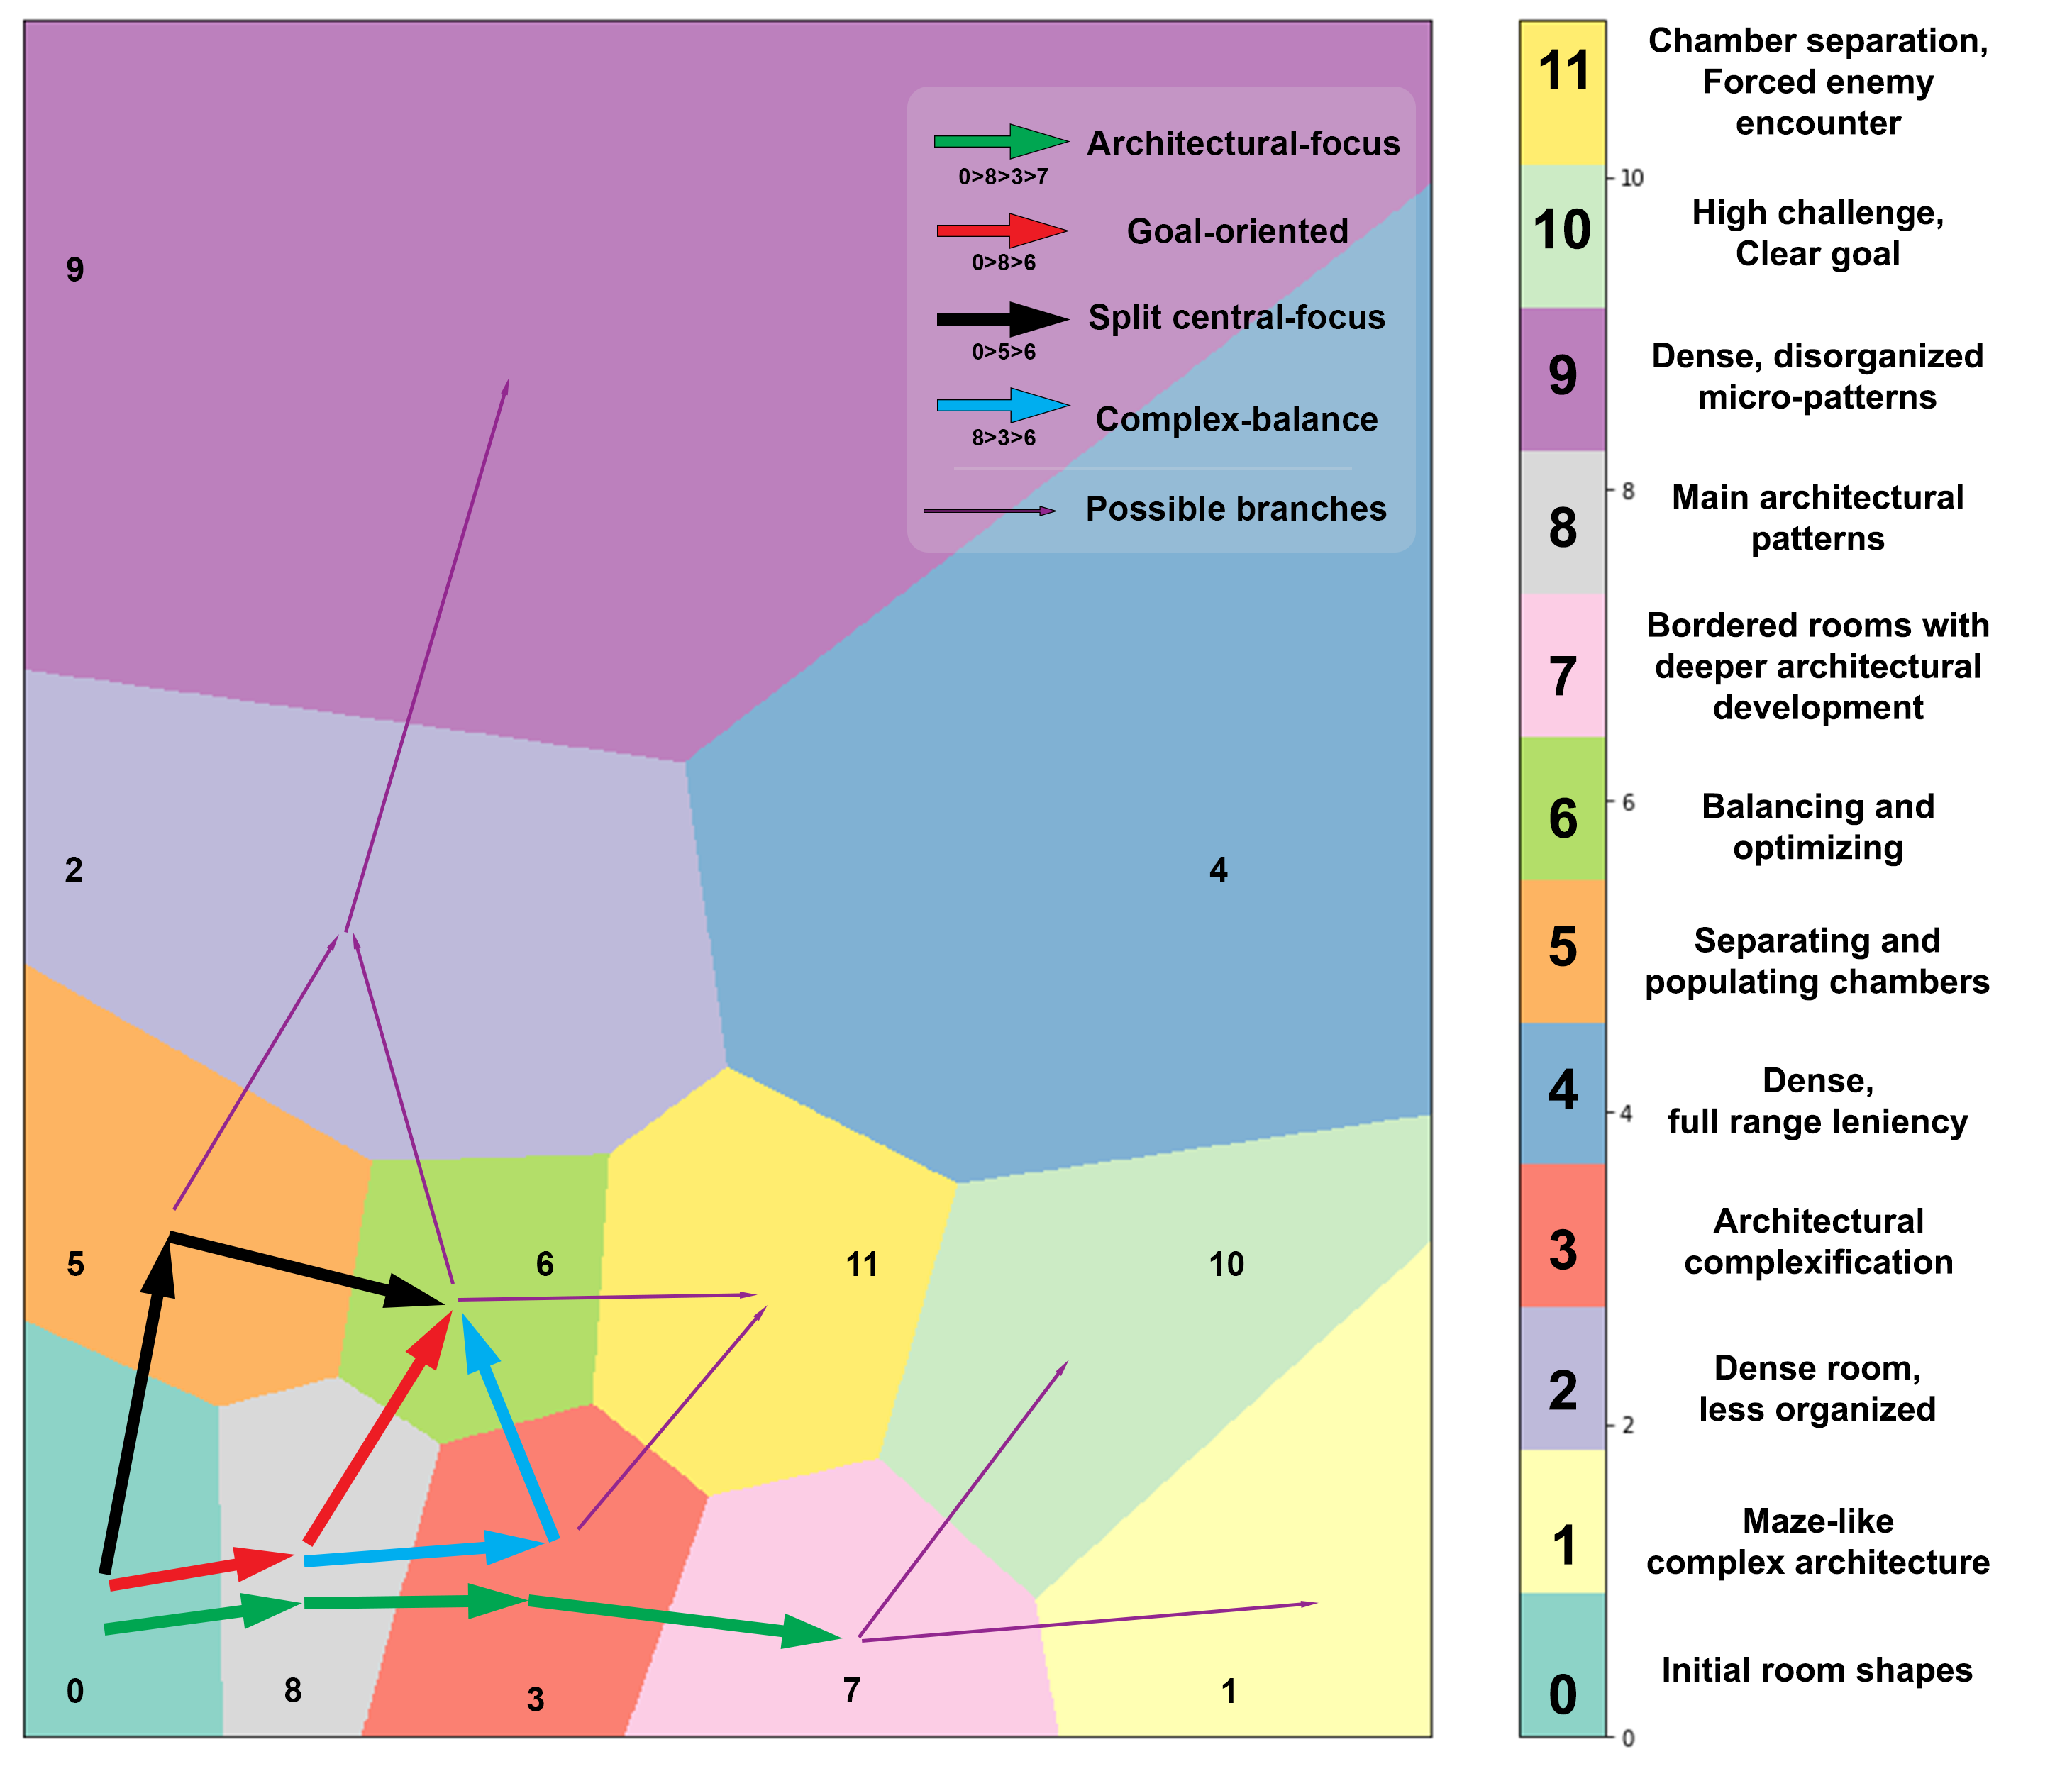
\includegraphics[width=\textwidth]{figures/DesPersonas-figs/resulting-paths-FINAL.png}}
\caption{Final and common designer trajectories. With thick arrows it is presented the archetypical paths, calculated using the frequencies of subsequences from $180$ diverse rooms. Each color represent a unique trajectory; with green the \textsc{Architectural-focus}, with red the \textsc{Goal-oriented}, with black the \textsc{Split central-focus}, and with blue the \textsc{Complex-balance}. Finally, thinner purple arrows extending from clusters traversed by the archetypical paths show the multiple possible branches that an archetypical path can deviate or extend to.} \label{fig:desPersonas}
\end{figure}

Moreover, with the design style cluster, we could then analyze the design process in function of the traversed clusters rather than evaluating each individual step. To do this, we analyzed the traversed clusters as unique trajectories. We gathered the common patterns from the trajectories by applying the Generalized Sequential Pattern (GSP) algorithm, which locates frequent subsequences in the analyzed trajectories. Through this, four \textit{designer personas} were identified. \textit{Designer personas} are defined as archetypical paths through style space that are commonly taken by designers when creating their content. In figure~\ref{fig:desPersonas} it is shown the identified \textit{designer personas}.
% , and figure~\ref{fig:desPersonasExamples} it is presented representative examples per each designer persona.

% \begin{figure}[t]
%     \centering
%      \subfloat[\textsc{Architectural-focus}\label{subfig-1:dummy}]{%
%       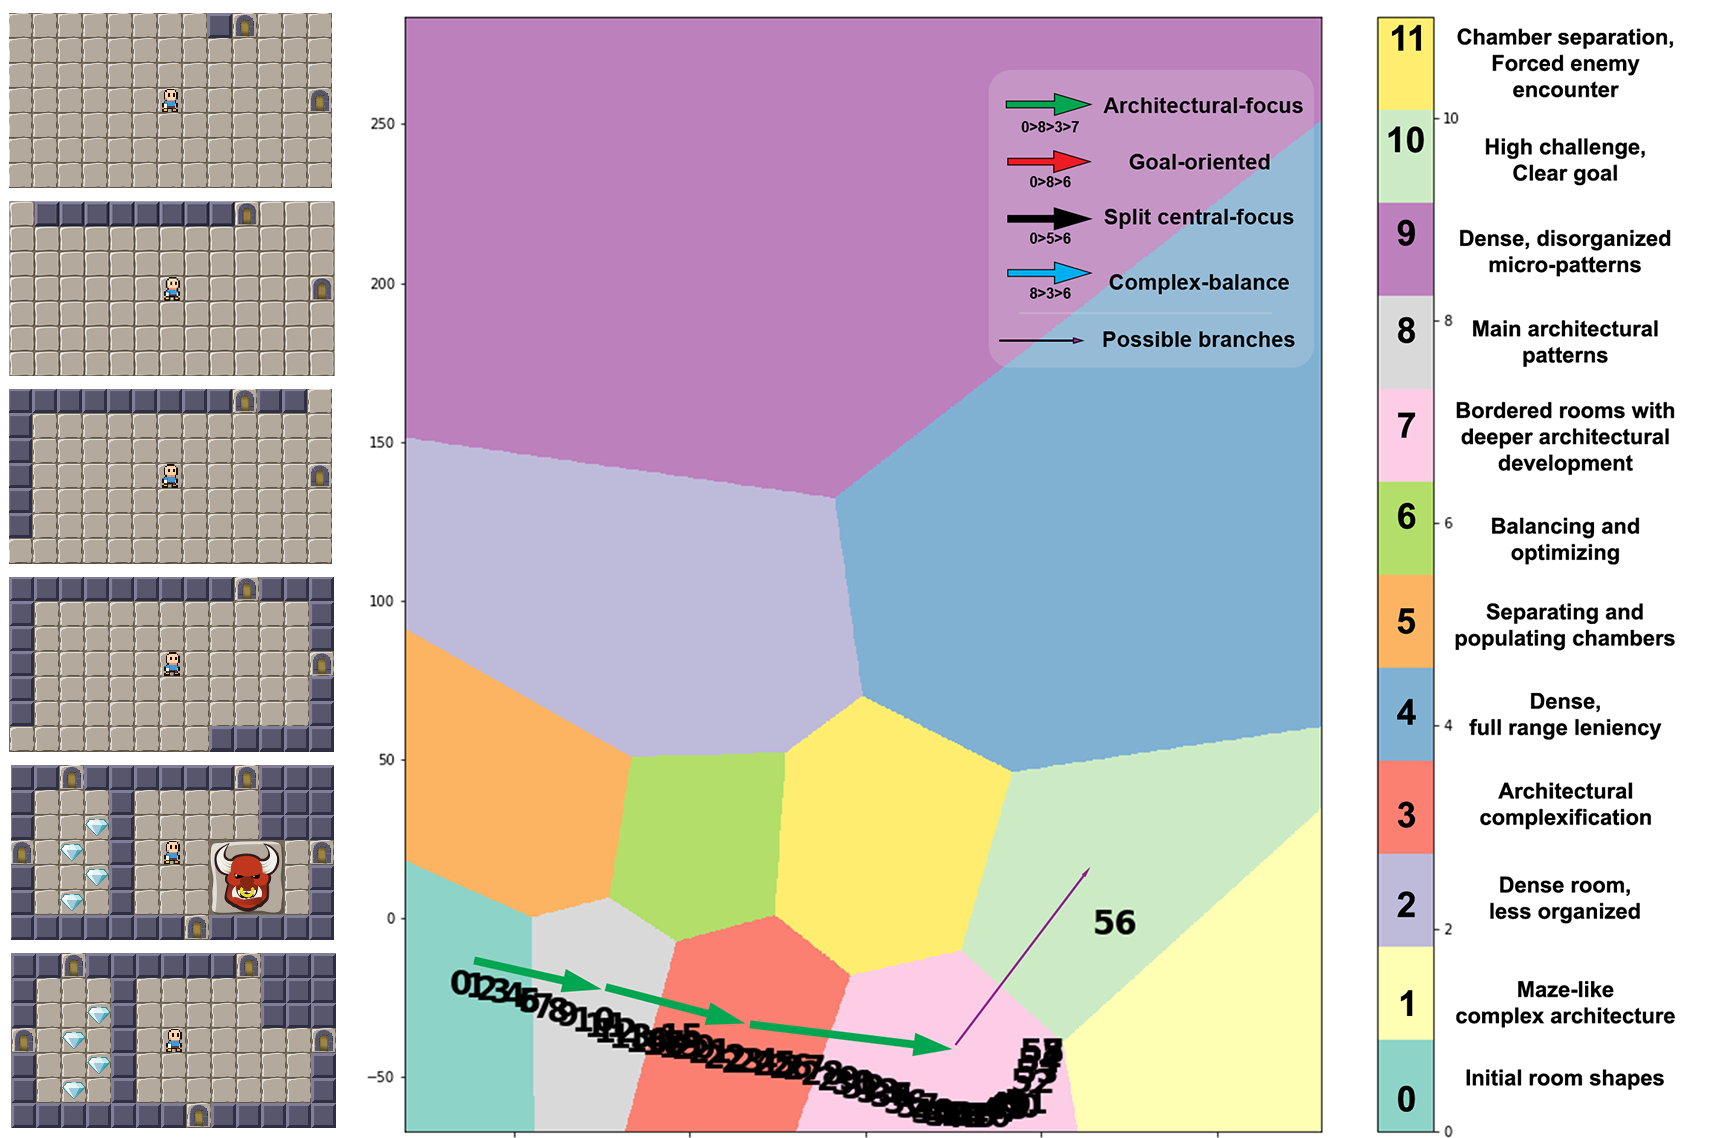
\includegraphics[width=0.6\textwidth]{figures/DesPersonas-figs/1.png}
%      }
%      \hfill
%      \subfloat[\textsc{Goal-oriented}\label{subfig-2:dummy}]{%
%       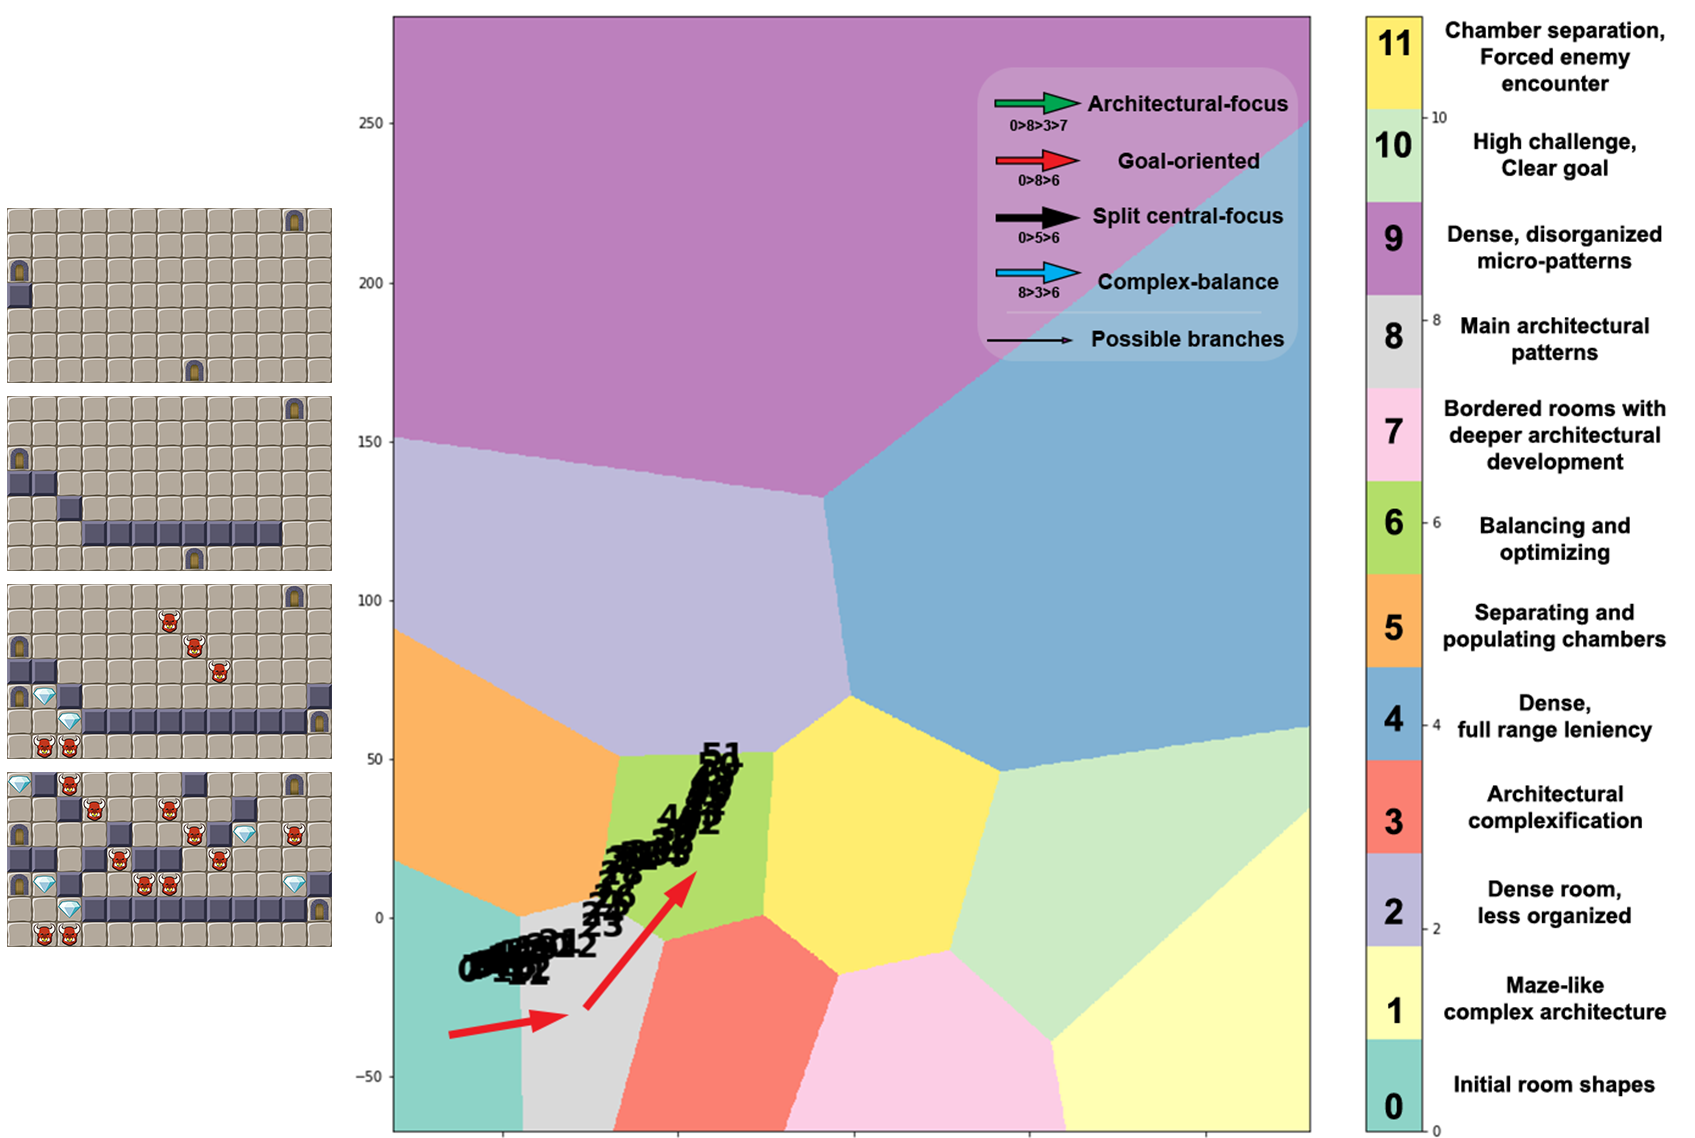
\includegraphics[width=0.45\textwidth]{figures/DesPersonas-figs/2.png}
%      }\hfill
%     %  \medskip
%      \subfloat[\textsc{Split central-focus}\label{subfig-3:dummy}]{%
%       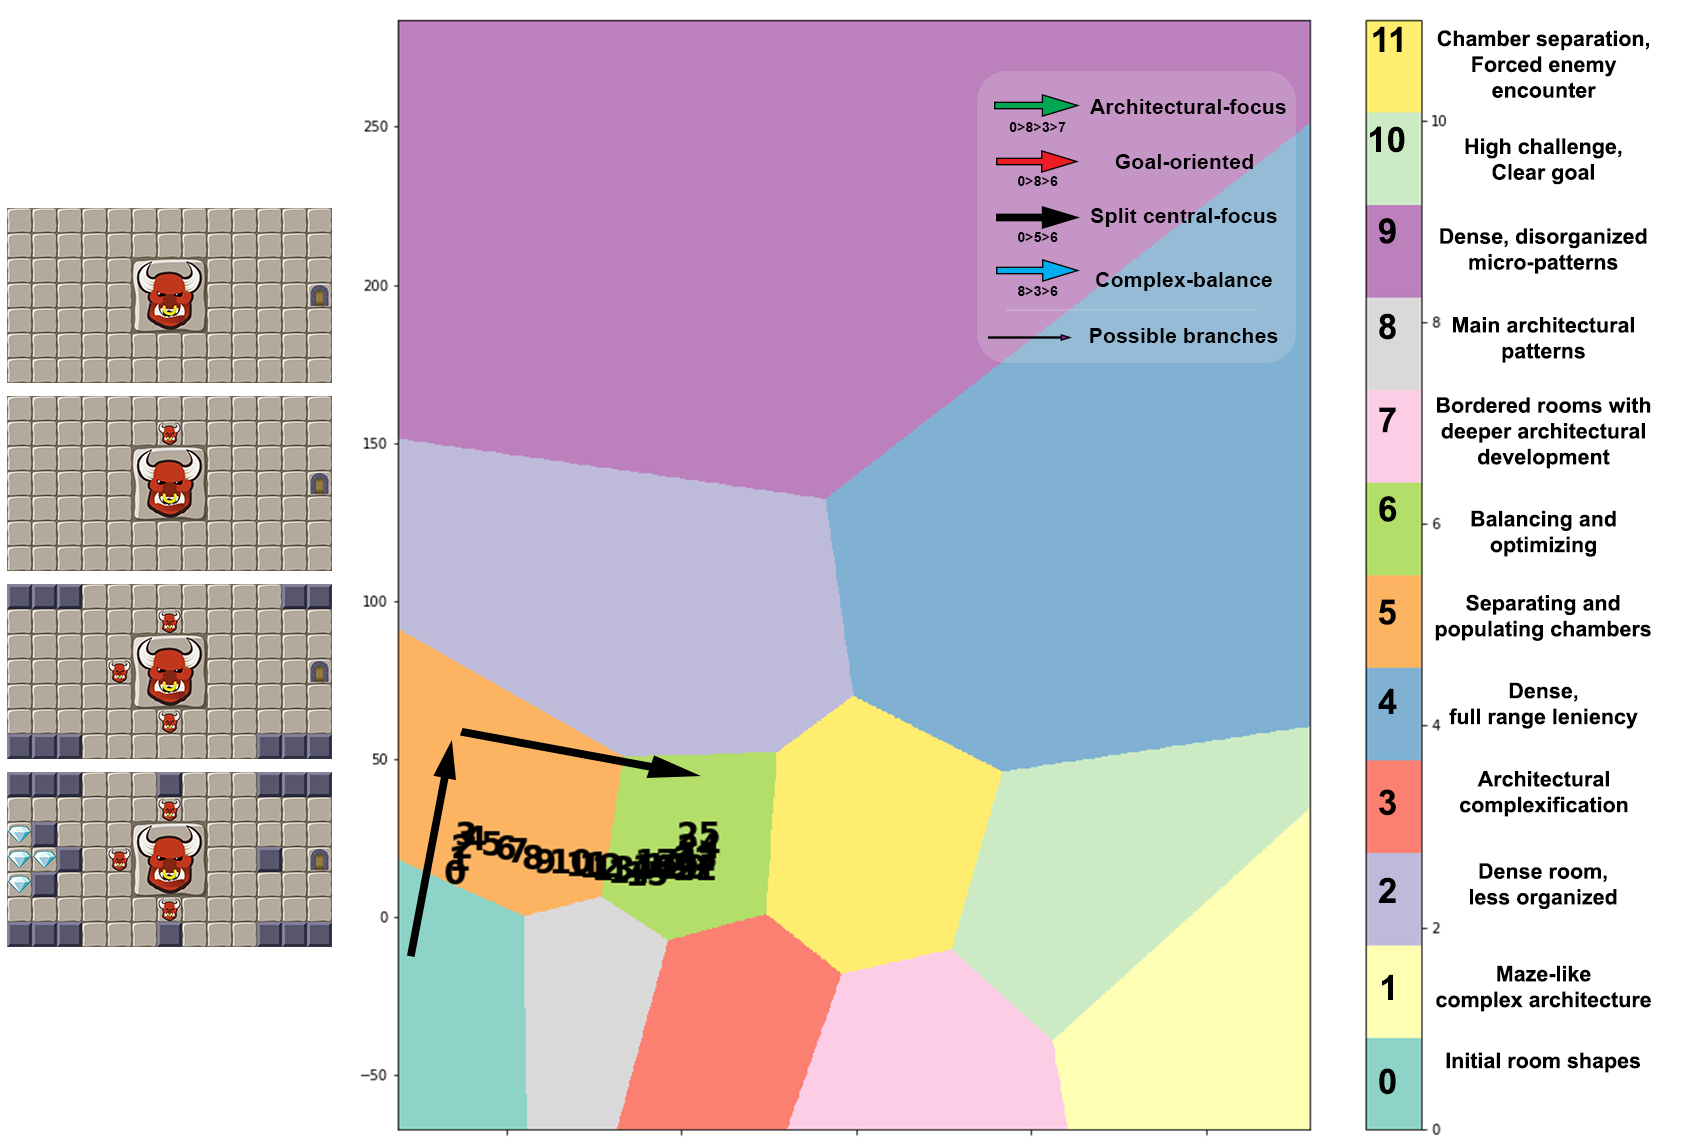
\includegraphics[width=0.45\textwidth]{figures/DesPersonas-figs/3.png}
%      }
%      \hfill
%      \subfloat[\textsc{Complex-balance}\label{subfig-4:dummy}]{%
%       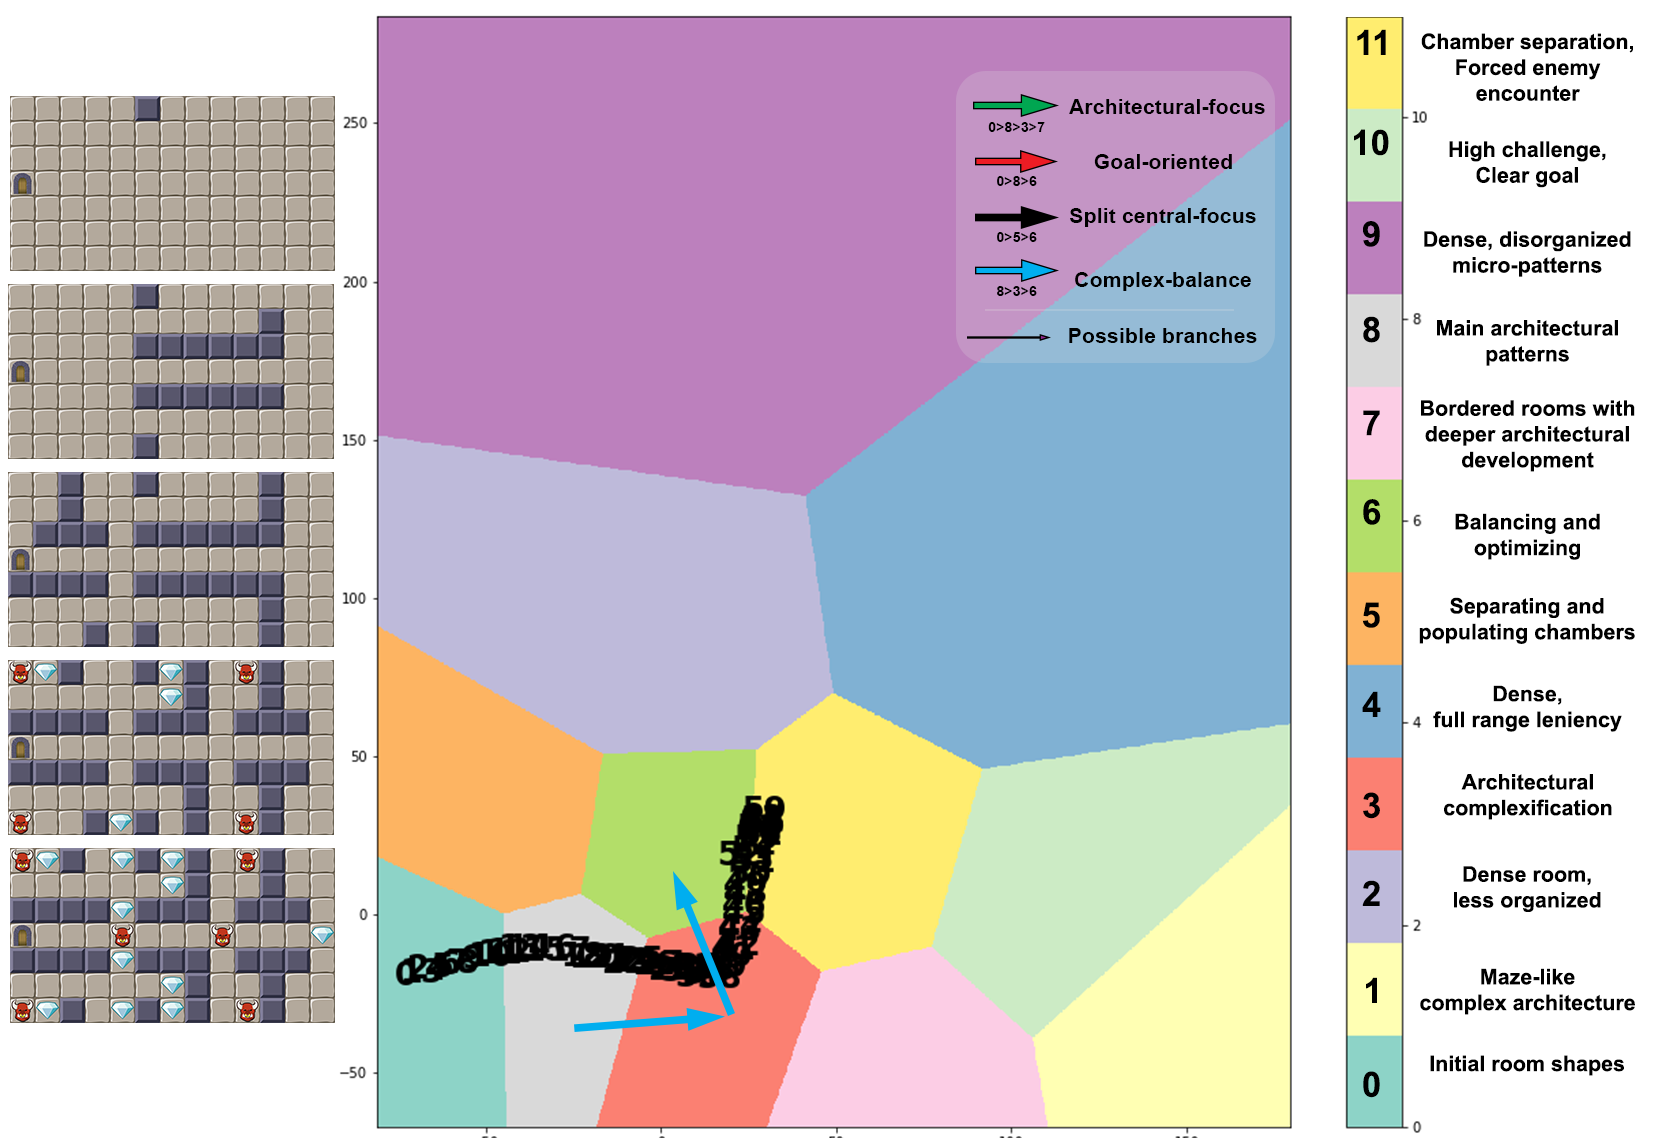
\includegraphics[width=0.6\textwidth]{figures/DesPersonas-figs/4.png}
%      }
    
%      \caption{Examples of each of the archetypical paths from one of the frequent sequences used to create the clusters. To the left of each subfigure, we present each key step in the trajectory i.e., when the design entered a new cluster. (a) presents the \textsc{Architectural-focus} archetypical path where the focus is firstly on creating the structural design of the rooms; the design process jumps back and forth suddenly to cluster 10 (one of the possible branches) due to the designer adding a boss and removing it immediately. (b) presents the \textsc{Goal-oriented} archetypical path where the design focus on a minimal structure complexity and mix between adding structural changes and enemies/treasures. (c) shows the \textsc{Split central-focus} archetypical path where, intentionally, the designer creates a center obstacle with a boss and build around it. Finally, (d) presents the \textsc{Complex-balance} archetypical path; the design focuses on building complex, uncommon structures first and then add some goal to it with enemies and treasures, taking advantage of the spaces.}
%     \label{fig:desPersonasExamples}
% \end{figure}

%\input{chapters/Algorithm_Adapt}
%\input{chapters/DesignerPersonaEvaluation}
\section{RESEARCH METHODOLOGY} \normalfont 
\label{sec:method}

This section describes the overarching research methodology, the methods used and how they were applied, a methodological reflection, and a discussion of other methodologies that were considered, and which are as valid for this thesis. 

%  Further, the nature of the thesis and the RQs require a mixed-method approach using both qualitative and quantitative methods.

To explore game design as a Human-AI collaborative task, how game content might be generated and adapted, and how to better integrate AI in these systems and processes, this thesis mainly follows a ~\acrfull{dsrm}~\cite{DSRM-Hevner}.~\acrshort{dsrm} aims at producing innovative artifacts to address a set of problems, challenges, and research questions within an area of concern. This thesis investigates this through a mix of qualitative and quantitative methods. Qualitative methods such as user studies, interviews, and controlled experiments, to collect data from usability, experience, and clarity of the interaction. Quantitative methods such as simulation and experimentation, where the goal is to evaluate specific properties, trade-offs, and the scope of the artifacts. 

Moreover, artifacts created for the purpose of creating technology-innovation, are categorized according to~\acrshort{dsrm} in the following four types: \emph{constructs}, \emph{models}, \emph{methods}, and \emph{instantiations}. \emph{Constructs} are the symbols and composed language to represent and define the problem and possible solutions. \emph{Models} are the representations of the problems and solutions, which uses the previously defined constructs. \emph{Methods} are the processes that are followed to solve the represented problem. Finally, \emph{instantiations} are the final systems used to demonstrate that the other categories can be used as solutions to address the defined problems~\cite{DSRM-Hevner}. Through the thesis, four artifacts have been developed.

% The first one relates more to the definition of \textbf{instantiation}

\subsection{Evolutionary Dungeon Designer}

the~\acrlong{edd}, defined as \textbf{instantiation}, is the main research tool in this thesis where we can investigate game design and multiple content creation aspects as well as the interaction between human designer and computational designer.~\acrshort{edd} has enough flexibility to explore this interaction and to use it as a research tool to investigate the performance, behavior, and usability of multiple AI techniques and models. Thus, by developing and evaluating~\acrshort{edd}, it is possible to support the development and creative expression of humans, and to test systems that aim at improving and exploring the co-creative, co-creation, and co-design capabilities of~\acrshort{micc}.

We have developed four systems that build on top of~\acrshort{edd} to explore this interaction.~\acrshort{edd} main content generation area is within level design, which is explored and developed in \textsc{papers i-iii, v, vi}. Within~\acrshort{edd}, we have also explored the generation of narrative, and its connection and usability alongside the level design facet. Narrative is explored and implemented in QuestGram (\textsc{paper vii}), TropeTwist (\textsc{paper x}), and Story Designer (\textsc{paper xi}).

% These four systems 

\subsection{Computational Designer}

The computational designer (composed of multiple AI techniques) related to \textbf{model, method, and instantiation}, where each underlying AI technique is implemented, used, and evaluated within~\acrshort{edd}. Through this, it is explored how different approaches affect the human-AI interaction, while aiming towards fostering creativity, reducing workload, and creating a much tighter Human-AI dynamic. These AI techniques range from addressing specific challenges such as explicit controllability by human designers and their aesthetic consideration (\textsc{paper ii}), to the use of quality-diversity algorithms to generate content in different facets (\textsc{papers iii, v, x, xi}), to the use of different type of grammars such as L-systems (\textsc{paper viii}) and graph grammars (\textsc{paper x}).

Furthermore, it is relevant to explore not only what algorithms and AI techniques are used for the Computational Designer, but also its role in the interaction. Thus, the role of the computational designer and its agency was preliminary explored in \textsc{paper xii}. We analyzed and evaluated through a controlled experiment in the form of user study, the interaction and user experience of the human designer when the computational designer gains more agency in the final design. 

\subsection{Temporal Expressive Range Analysis}

%\begin{itemize}
%    \item Explain briefly ERA
%    \item Explain TERA and how it can be used. Why was it proposed? what was missing that needed it?
%    \item Paper I present this and when/where I used 
%\end{itemize}

Expressive Range Analysis (ERA) is a popular and relevant method to evaluate content generators, since it allows the inspection of the diversity and expressiveness of a content generator with regards to feature dimensions and use as a comparison with other algorithms~\cite{shaker_procedural_2016,cook_danesh_2016,horn_comparative_2014}. In \textsc{paper viii}, we extended ERA and presented Temporal Expressive Range Analysis (TERA) as a method to better use ERAs in interactive PCG and MI-CC systems. TERA relates in DSRM as a \textbf{method}, and is proposed as a evaluation method to analyze and assess theses interactive systems. TERAs allow the inspection and analysis of changes in the ERA over a defined period such as generations, design editions, or time; and how the algorithms react and adapt to constant changes in the input. We introduced an aggregated and non-aggregated version. Non-aggregated TERAs show the delta maps of the generator, meaning where the generator has focused and the space covered for a specific period part. Aggregated TERAs show the density of generated content over all the defined period and the coverage up to the specific period. TERAs were used in \textsc{papers viii and xi} to assess the content generated with the IC MAP-Elites for game levels and narrative structures. 

%as presented in the background (), is a common and relevant method to evaluate content generator, especially in PCG, since it allows the inspection of the diversity of a content generator with regards to feature dimensions. 

%The following cases examine TERAs following the different scenarios presented in figure~\ref{figs:roomsexperiments}. Different cases will use either an aggregated TERA step by step or a non-aggregated version showing each step's specific scores in the evaluated dimensions. Each figure's caption and respective case will indicate what type of TERA is used. Non-Aggregated TERAs show the delta maps in the search, meaning where the search has focused and the space covered for a specific step. On the other hand, aggregated TERAs show the density of generated individuals over all steps and the coverage up to the specific step. In each TERA, we also show as an orange dot where the current design is in relation to the used and tested dimensions. Case 1 and 2 examine aggregated TERAs, while case 3 examines non-agreggated TERAs.

%Therefore, the contributions of this paper are two-fold. On the one hand, we present Temporal Expressive Range Analysis (TERA) as a novel way to analyze interactive PCG. TERAs allow us to inspect and analyze the changes in the expressive range over a defined period, which in our case, are design editions. On the other hand, using TERAs, we explored and analyzed how population dynamics react and adapt to constant changes in the IC MAP-Elites for level generation of 2D adventure games.

\subsection{Designer Personas}

In this thesis, we argue about the importance of \emph{Designer Modeling} in MI-CC systems as a step towards adaptability, tailor-made experiences, and better interactions. We approached and investigated this in \textsc{papers iv and ix}. Nevertheless, in \textsc{paper ix} we presented and proposed an approach, related in DSRM as a \textbf{method}, for a data-driven modeling of the design process, style, and goals. This method allows for the identification of \emph{Designer Personas} as archetypical paths through a clustered design style space in the respective design space. \emph{Designer Personas} take the task of recognizing style and adapting content towards that to a higher abstraction layer, where both the final design and individual design edits are less relevant, and the process and trajectory through a clustered style space based on designer's data is highlighted.  For instance, rooms for a game like the binding of Isaac~\cite{mcmillen_binding_2011} could be classified based on multiple characteristics such as the room's objectives regarding enemies and treasures, access to different areas, or hidden encounter and treasures. Moreover, different designers could reach the same room style through different paths, where the focus along the creation could vary. Some designers would focus on the room's architecture before anything else, whereas others would focus first on the objectives a player must achieve.

%In this thesis, we argue about the importance of \emph{Designer Modeling} in MI-CC systems as a step towards adaptability, tailor-made experiences, and better interactions. We approached and investigated this in \textsc{paper v, x, and xiv} and as part of this kappa's contribution. Nevertheless, in \textsc{paper x} we presented and proposed an approach, related in DSRM as a \textbf{method}, for a data-driven modeling of the design process, style, and goals. This method allows for the identification of \emph{Designer Personas} as archetypical paths through a clustered design style space in the respective design space. \emph{Designer Personas} take the task of recognizing style and adapting content towards that to a higher abstraction layer, where both the final design and individual design edits are less relevant, and the process and trajectory through a clustered style space based on designer's data is highlighted.  For instance, rooms for a game like the binding of Isaac~\cite{mcmillen_binding_2011} could be classified based on multiple characteristics such as the room's objectives regarding enemies and treasures, access to different areas, or hidden encounter and treasures. Moreover, different designers could reach the same room style through different paths, where the focus along the creation could vary. Some designers would focus on the room's architecture before anything else, whereas others would focus first on the objectives a player must achieve.

%where individual design edits are less relevant ... is not only an alternative method for designer modeling, but it can be used not 

%An alternative method could be to identify a set of styles that most designers follow when creating content, and model how the designer traverse such a style space. For instance, rooms for a game like the binding of Isaac~\cite{mcmillen_binding_2011} could be classified based on multiple characteristics such as the room's objectives regarding enemies and treasures, access to different areas, or hidden encounter and treasures. Moreover, different designers could reach the same room style through different paths, where the focus along the creation could vary. Some designers would focus on the room's architecture before anything else, whereas others would focus first on the objectives a player must achieve. These designer models could then be combined with search-based~\cite{Togelius2011} or other procedural generation methods~\cite{khalifa2020-pcgrl,Volz2018-GANevo} to suggest ways of getting to the next design style from the current one. 

%\begin{itemize}
%    \item Designer personas method? I don't know if that makes that much sense, men I should check
 %   \item Paper I present this and when/where I used
%\end{itemize}

% Furthermore, it is relevant to explore not only what algorithms and AI techniques are used for the Computational Designer, but also its role in the interaction. 


% In MI-CC, the human is mostly in control of what will and can be created, 


% in Mixed-Initiative Co-Creative tools, the human is mostly in control of what will and can be created, delegating the AI to a more suggestive role instead of a colleague in the co-creative process. Allowing more control and agency for the AI might be an interesting path in co-creative scenarios where AI could direct and take more initiative within the co-creative task. However, the relationship between AI and human designers in creative processes is delicate, as adjusting the initiative or agency of the AI can negatively affect the user experience. In this paper, different degrees of agency for the AI are explored within the Evolutionary Dungeon Designer (EDD) to further understand MI-CC tools. A user study was performed using EDD with three varying degrees of AI agency. The study highlighted elements of frustration that the human designer experiences when using the tool and the behavior in the AI that led to possible strains on the relationship. The paper concludes with the identified issues and possible solutions and suggested further research.


% it


% while others addresses several RQs such as developing designer models (\textsc{paper vi}).

\subsection{Methods}

All the publications included in this theses have followed some of the possible design evaluation methods introduced by Hevner et al., which are categorized into observational, analytical, experimental, testing, and descriptive~\cite{DSRM-Hevner}. Thus far, the focus has been on doing analytical, experimental, and descriptive methods, with a mix of quantitative and qualitative data collection.

The systems were evaluated with \emph{analytical} and \emph{experimental} methods. Analytically through a dynamic analysis to evaluate qualities such as performance and expressiveness. Experimentally through simulation with artificial and meaningful data to, for instance, analyze the exploration capabilities, reactiveness, interaction, and adaptability of the algorithms. The ~\emph{dynamic analysis} focused on performing expressive range analysis and temporal expressive range analysis (\textsc{papers iii, v, viii, xi}). The \emph{simulation} has focused on evaluating how the tool responds to different inputs and the robustness of algorithms with noisy and unpredictable data such as in~\textsc{papers iii, vii, or xi}.

Moreover, ~\emph{controlled experiments} in the form of user studies have also been conducted to collect qualitative data on how the focus group (i.e., game designers) experience and use the tool. Through this, informed decisions can be taken on focus areas that might be important and relevant to explore as shown in the results of~\textsc{papers i, iv, vii, ix, xii}. 

%and~\textsc{paper vi}.% This thesis must conduct these user studies regularly to investigate these areas, and to determine if the interactions that we want to establish and the capabilities and experiences that we are expecting to improve and foster do indeed work as expected.

Finally, Hevner et al.~\cite{DSRM-Hevner} recommended the use of ~\emph{descriptive} methods only when innovative artifacts cannot be evaluated using any of the other evaluation methods. Therefore, having in mind that this is still an unexplored research area, descriptive methods such as \emph{Informed Argument} are required to build support for an artifact's necessity, challenges, and applications. For instance, the method and model developed in~\textsc{paper ix}, used data from user studies that resulted in the clsutering of the design space into design style clusters. We further used this to explore and identify Designer Personas.


%, yet its evaluato explore archetypical design paths, namely Designer Personas.



% \subsection{Objective iterations}

% The work in this thesis is divided into two parallel artifacts,~\acrshort{edd}, the main research tool used, and the computational designer (composed of multiple AI techniques). Furthermore, visualizing these artifacts through the~\acrshort{dsrm} iteration cycle, makes it clear that both artifacts can be represented as parallel and independent iterations, while naturally, sharing common sub-parts. In the following subsections, these iterations are presented as individual cycles, as well as within overarching objectives.

% \subsubsection{Focus in the evolutionary algorithm to explore interaction with varying degree of control.} The objective with these studies and experiments is to explore how control can be given to designers through interacting and working directly with the the~\acrlong{ea}.

% \begin{figure}
% 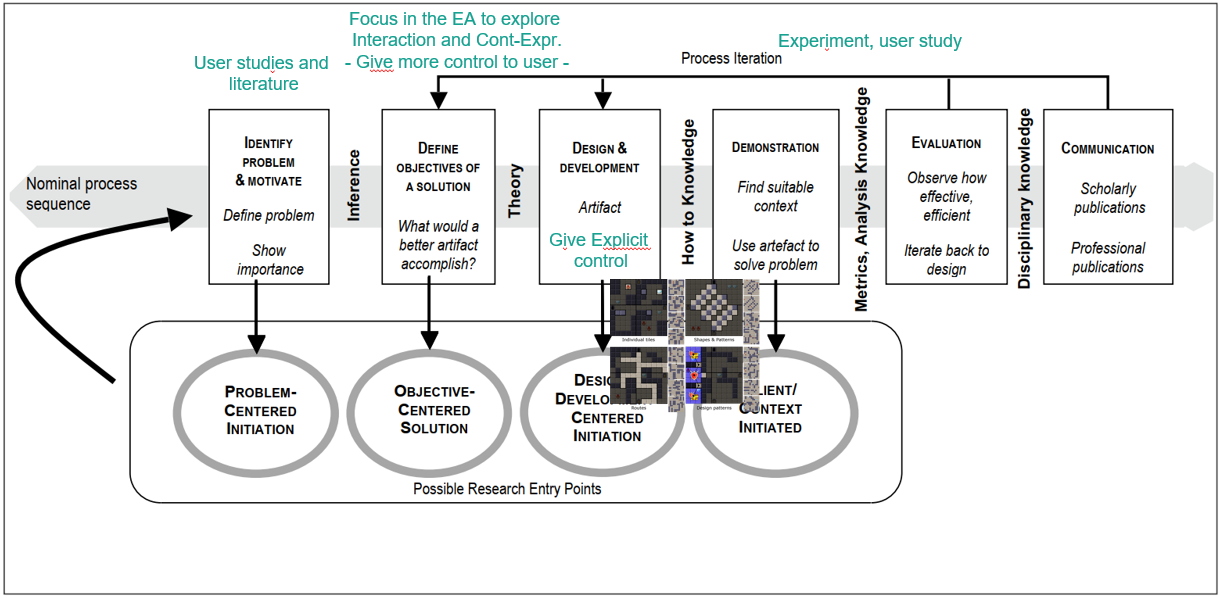
\includegraphics[width=\textwidth]{figures/Methodology-figs/lockingtiles-dsrm.png}
% \caption{DSRM cycle of the first study~\cite{Alvarez2018a}} \label{figs:lockingTiles}
% \end{figure}

% Figure~\ref{figs:lockingTiles} shows the first DSRM process seeking the development, exploration, and evaluation of providing direct control over multiple steps in the EA i.e. crossover and mutation, through locking tiles that needed to be preserved~\cite{Alvarez2018a}. For this process, two iterations were performed, one to evaluate the artifact through simulations to study to what extent the approach was controlling the evolutionary process. The second iteration focused on evaluating the approach's usability and assessing how designers interacted with the systems and responded to the suggestions. The solutions were deemed positive, but the expressivity of the algorithm was affected, and the workload of designers increased to some extent, given that they needed to provide what was to be preserved.

% \begin{figure}
% 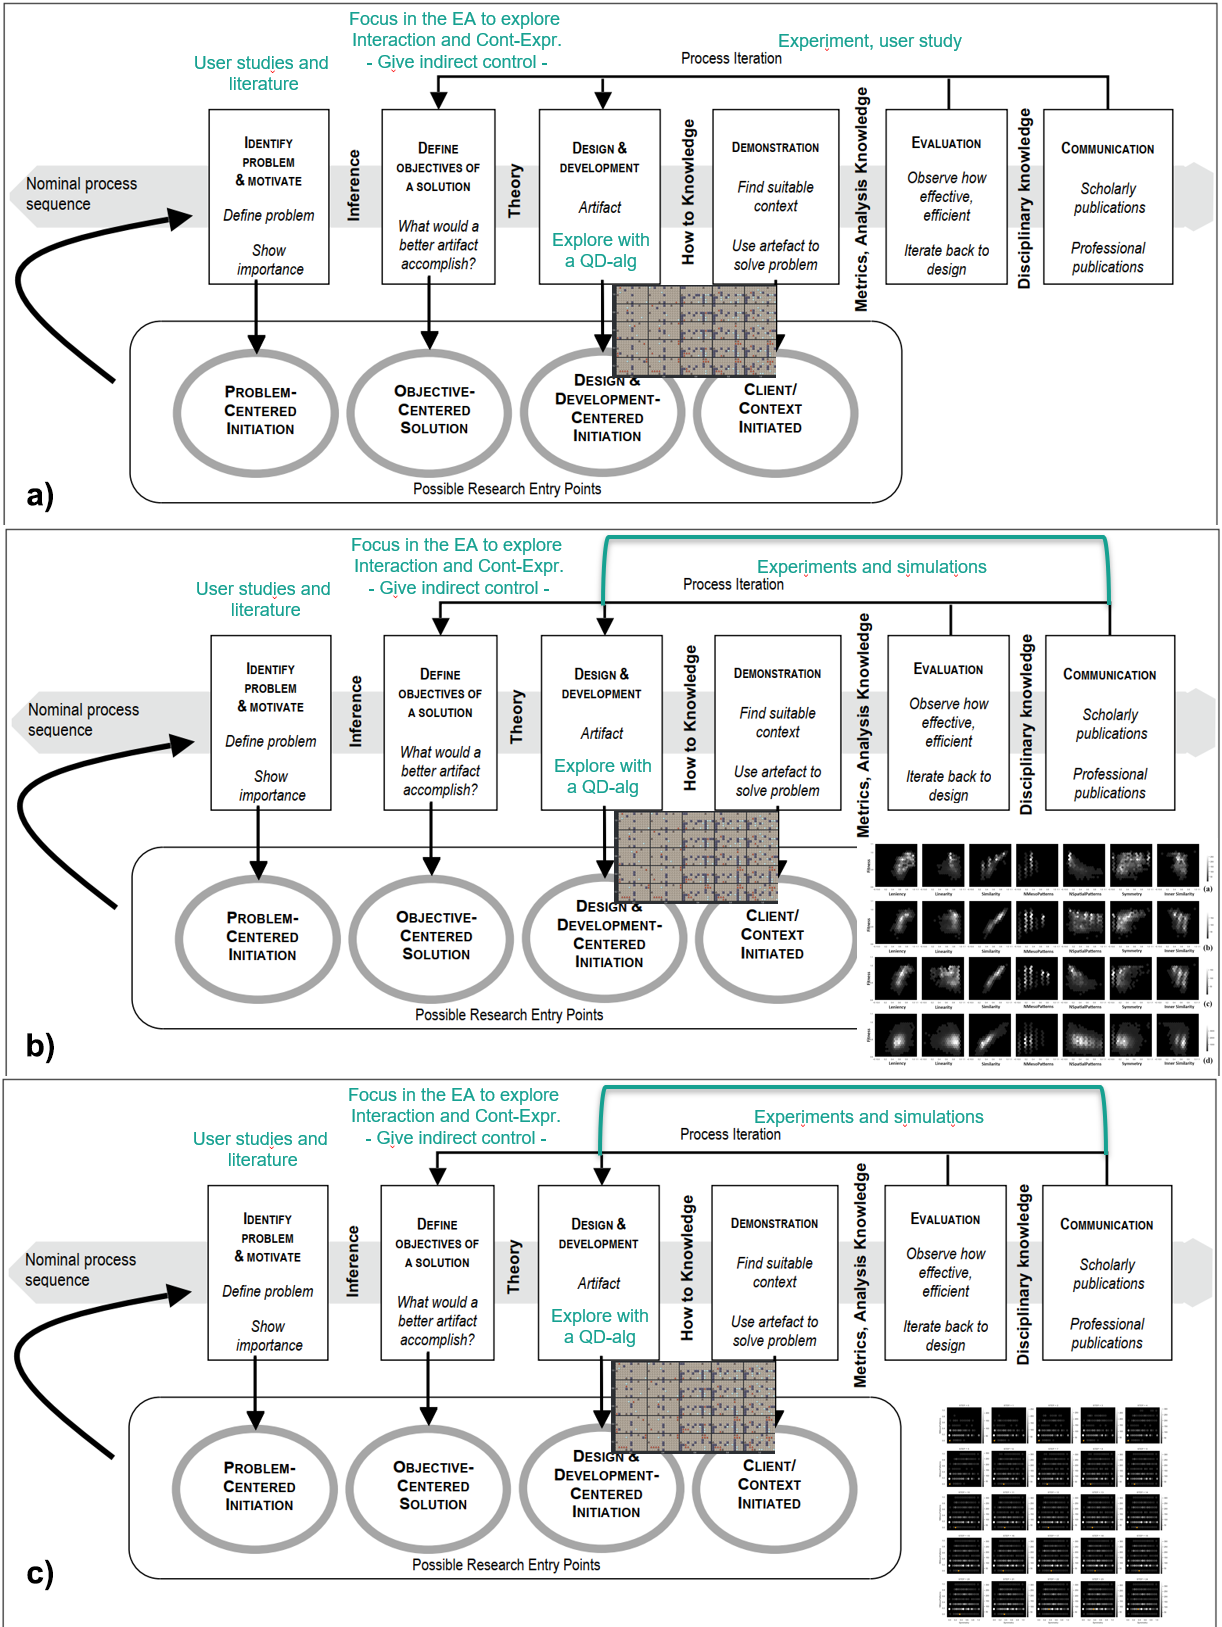
\includegraphics[width=\textwidth]{figures/Methodology-figs/ICMAPE-dsrm.png}
% \caption{DSRM cycle of the second study~\cite{alvarez2019empowering}. a) denotes the first and second iteration~\cite{alvarez2019empowering}, b) the third iteration where the evaluation was on static levels~\cite{Alvarez2020-ICMAPE}, and c) the fourth and current iteration where IC MAP-Elites was evaluated in a dynamic environment~\cite{Alvarez2020-ICMAPE-interactive}.} \label{figs:icmape}
% \end{figure}

% Moreover, informed by the user study evaluating the tool and it is new features and underlying-AIs~\cite{Alvarez2018}, a new DSRM process was started. In figure~\ref{figs:icmape}, it is shown this parallel cycle within the same objective, exploring interaction with the EA. The focus of this process was to study how to use Quality-Diversity (QD) algorithms to balance controllability and expressivity due to the special properties of these algorithms, where the focus is on searching a substantial area of the solution space while yielding high-performing individuals~\cite{gravina2019procedural,Pugh2016}. Therefore, the development was set into producing a variant of a recent and popular QD algorithm called MAP-Elites~\cite{Mouret2015}. The proposed approach named Interactive Constrained MAP-Elites (IC MAP-Elites)~\cite{Alvarez2020-ICMAPE}, is a variant of the Constrained MAP-Elites, introduced by Khalifa et al.~\cite{Khalifa2018}, combined with Interactive Evolution.

% The algorithm yielded very positive results, and have had most of the focus in this thesis. The process is still on-going, and four iterations have been done. The first (fig. ~\ref{figs:icmape}.a), when the algorithm was proposed~\cite{alvarez2019empowering}, evaluated through simulations the properties of QD algorithms, and the possibilities it brings. The second iteration focused on evaluating IC MAP-Elites through controlled experiments with an informal user study. Designers were asked to try the tool without special focus in the QD algorithm, but rather as a more general test. The results from such a study informed the next DSRM process focused on modeling designers. Moreover, the third and fourth iterations (fig. ~\ref{figs:icmape}.b and .c, respectively), focused on a dynamic evaluation of IC MAP-Elites to identify and explore the generative space of the algorithm and its properties and dynamics in both, a static scenario using all pair of dimensions~\cite{Alvarez2020-ICMAPE}, and dynamic one following simulations of the MI-CC interactive loop~\cite{Alvarez2020-ICMAPE-interactive}.
% %This process is still on-going, and two iterations have been done—the first when the algorithm was proposed.

% \subsubsection{Focus in moving towards designer modeling through different adaptive models.} While the previous DSRM cycle is not over yet, conducting those studies pointed out key directions to focus and new aims to address the above-mentioned RQs. The objective with the following cycles is to explore ways towards designer modeling. This in order to reduce the designer's fatigue and create better and adaptive experiences that take into consideration an individual's preferences, styles, and in general, their design and creative process.

% \begin{figure}
% 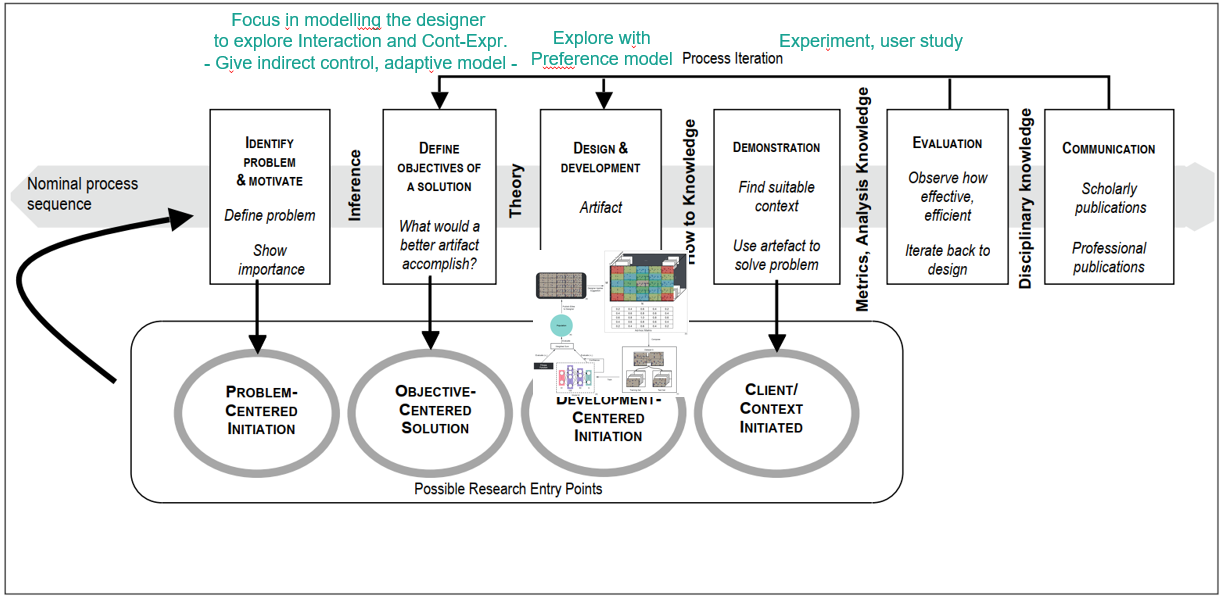
\includegraphics[width=\textwidth]{figures/Methodology-figs/desPref-dsrm.png}
% \caption{DSRM cycle of the third study~\cite{Alvarez2020-DesignerPreference}.} \label{figs:desPrefDSRM}
% \end{figure}

% \begin{figure}
% 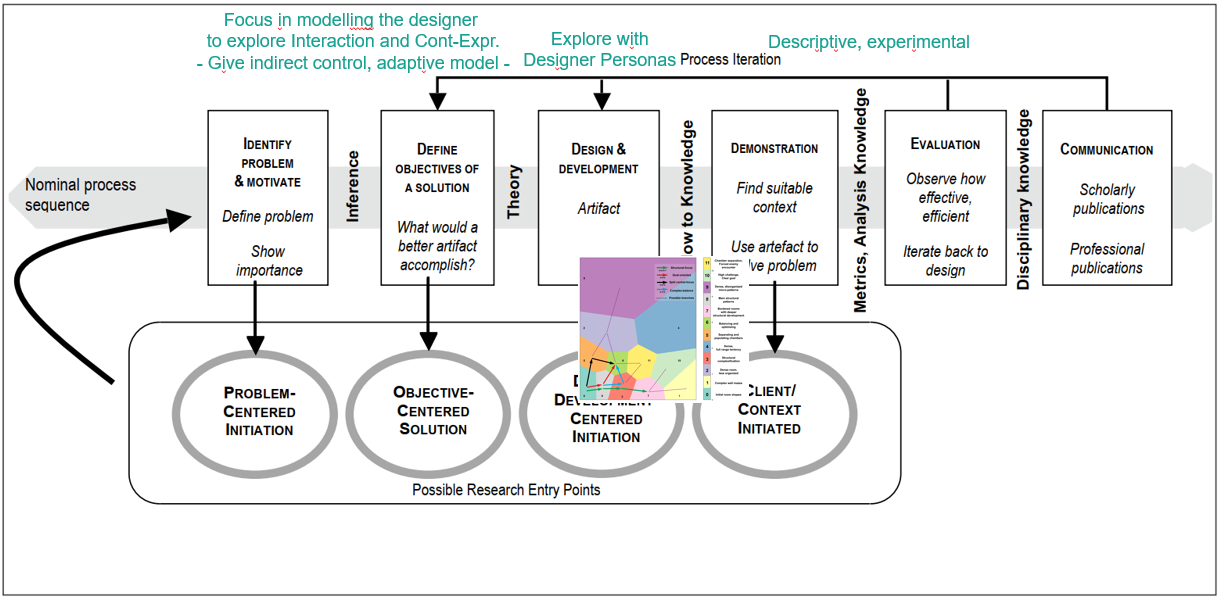
\includegraphics[width=\textwidth]{figures/Methodology-figs/desPersonas-dsrm.png}
% \caption{DSRM cycle of the fourth study~\cite{alvarez2020-designerpersonas}.} \label{figs:desPersDSRM}
% \end{figure}

% Figure~\ref{figs:desPrefDSRM} presents the first cycle towards designer modeling by exploring the usage of a preference model~\cite{Alvarez2020-DesignerPreference}. In this model informed by the findings in ~\cite{alvarez2019empowering,Alvarez2018}, and the unpublished user study of the IC MAP-Elites, the focus was on automatically modeling the preferences of the designer. This was done by collecting new data as the designer was applying suggestions by the EA, and training a neural network (ANN) with the distribution of the provided suggestions. Figure~\ref{figs:desPrefModel} exemplify the procedure. Furthermore, the preference model went through two iterations, the first, where the model i.e. ANN, was evaluated to explore the accuracy and usability, and a second, where the model was tested in practice by beginner designers.

% Moreover, figure~\ref{figs:desPersDSRM} presents another cycle within the frame of adaptive models. In this case, the focus was on dividing the design space to form clusters of room styles based on the data collected from previous user studies. Analyzing the designer's edition steps when using the tool in relation to the new clusters, the study identified four archetypical paths taken by most designers, named Designer Personas~\cite{alvarez2020-designerpersonas}. The contribution was evaluated through descriptive methods because while data was used to form the Designer Personas, its usability and support are informed by literature.

\subsection{Methodology Discussion}

This thesis embraces~\acrshort{dsrm} as the principal methodology employed to explore, analyze, and address the different artifacts and RQs. However, it is essential to have a methodology discussion for those methodologies that could have been as valid in the frame of this thesis, with their own set of tradeoffs. 

%Before moving towards the different evaluation methods followed so far and that I have identified as necessary to address my RQs, I would like to bring the attention to other methodologies that could be as valid as well in the frame of this thesis. 

The field of Human-Computer Interaction (HCI) has studied for a long time the ways interactions can be created, approached, and established to foster, encourage, and address different functionalities and capabilities of humans. Likewise, the interaction between humans and AI has been the focus of much of the recent work by the community, which is now developing further than the computer science and information system frontiers towards intertwining with many other science fields~\cite{rahwan_machine_2019}. 

However, these interactions, especially when the human and the AI do not necessarily need to have asymmetric functionalities (i.e., having an intelligent system that merely assist) and that both can participate in reciprocal stimuli to reach a common goal, still have uncountable challenges and questions to research and explore. This is thus, one of the motivations behind this thesis, which in part calls for the use of a more exploratory and holistic methodology that can then observe, analyze, model, and address the unknown space of problems and solutions.

An exploratory methodology that could have been used is~\acrfull{rtd}~\cite{rtd-zimmerman2007} since, after all, the iterative design of multiple artifacts and the investigation of how this open new spaces in the research is important to understand those unknown spaces.~\acrshort{rtd} is a methodology from the field of~\acrshort{hci}, which aims at tackling ``Wicked Problems’’ meaning unexplored, unclear, and complex scenarios and situations that are not easily simplified.~\emph{Design Thinking} is the design process used to describe~\acrshort{rtd}, consisting of \emph{grounding, ideation, and iteration}. Following the~\acrshort{rtd} methodology, one addresses these problems through a holistic approach with an iterative process that reframes the problem through designing artifacts and prototypes as a means of knowledge. The knowledge generated from these prototypes reframes the space of problems and solutions, which in turn provides an important opportunity for researchers on focusing in the future state and on defining a preferred state to be achieved~\cite{rtd-critique-zimmerman2010}. 

Moreover,~\acrfull{pd} matches as well the requirements of this thesis, especially understanding that the research while focusing on the development of technological innovations and artifacts, has a human-centered perspective~\cite{ParticipatoryDesign-Spinuzzi2005}.~\acrshort{pd} is a methodology that involves the target user of a specific type of design in the design and research process. Through this, the necessities of the target user are gathered, and their visions, expertise, and understanding are incorporated and included in the proposed solutions. Usually, the researcher wants to explore certain aspects of an unknown space, although it is not necessary to be unknown, together with the target users. These users understand and manage different problems and solutions in the design space, thus by co-designing the solution, they are involved and are part of the solution rather than this being delivered to them~\cite{ParticipatoryDesign-Spinuzzi2005}. 

%I need to check a bit more this methodology. Furthermore, Björgvinsson et al \cite{bjorgvinsson-democratizing-innovation} coined the term ``democratizing innovation’’ to further connect participatory design results  the 

These methodologies could allow the work to be, in principle, more exploratory and letting the users actually participate in the design of the human-AI interaction loop. However, through the methods within~\acrshort{dsrm} and the research plan, this thesis has explored to a certain extent the incorporation of important aspects of these methodologies. While the main focus is on~\acrshort{edd} to explore this interaction; throughout this thesis, multiple prototypes and artifacts addressing the underlying AI have been developed to explore different design capabilities and interactions that have helped reframed problems and space of solutions, akin to~\acrshort{rtd}.

Furthermore, we have managed to evaluate qualitative aspects of the tools and the interaction designers have with it through user studies. Thus, from our focus groups (i.e., game designers), there are important points to approach and address that motivates the next steps in the thesis. For instance, in the user study done in~\textsc{paper i}, it was a recurrent topic that designers wanted more control over the tool and algorithms. Designers did not see a relation between their work and what the tool offered (i.e., preserving their design, intentions, and ideas), while of course, still expecting interesting solutions from the algorithm. This topic, supported by previous research, have chained a set of improvements and implementations in order to balance the requirements from designers. For instance, in~\textsc{papers iv, ix}, and in general, the steps towards capturing and developing designer models to be used as a complement evaluation in the interaction between the designer and the artificial design, have been motivated by the struggle and balance between controllability and expressivity.  

% \begin{figure}
% 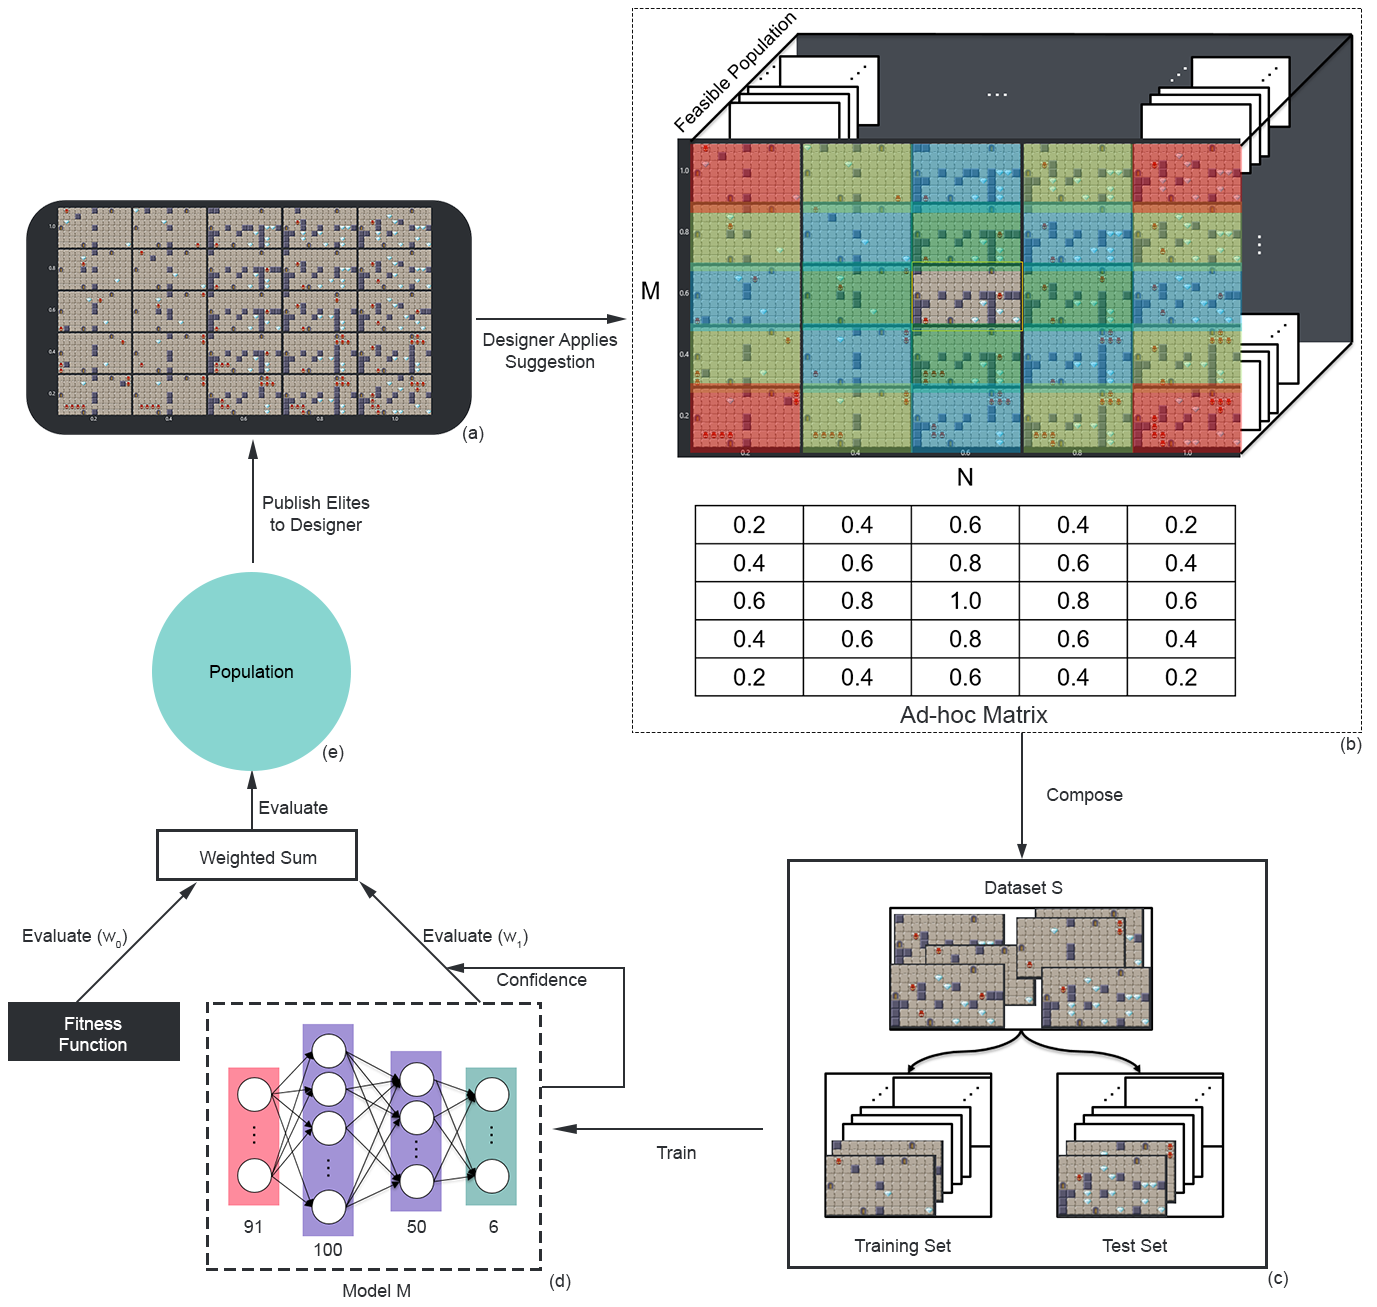
\includegraphics[width=\textwidth]{figures/fig4.png}
% \caption{Overview of the Designer Preference Model integrated into the fitness function of EDD. Elites are published and shown to the designer in a grid fashion (a), and once the designer chooses and applies one of the suggestions, an ad-hoc matrix is created based on the position of the selected suggestion to estimate the preference of suggestions (b). The ad-hoc matrix is then applied to all the elites in the grid, and the feasible populations within the EA cells to compose a general dataset $S$ with rooms labeled by the estimated preference. The composed dataset $S$ is then subdivided into a training set (90\%) and test set (10\%), both with the same label distribution (c). The dataset is used to train a model $M$, which is a relatively small neural network, for 20 epochs (d). The  model is then used to evaluate the population of the EA together with the current fitness function in a weighted sum, with the weight of the model $M$ conditioned by the confidence of the network (e).} \label{figs:desPrefModel}
% \end{figure}




\section{CONTRIBUTIONS} \normalfont

%\setlength{\epigraphwidth}{2in} 
%\epigraph{\textit{It's a kind of magic}}{Queen, A Kind of Magic.}

%\setlength{\parindent}{0.0em}

This section summarizes the research contributions of the publications that this thesis compiles and unifies. First, contributions and publications are linked to different RQs. Then, each RQ is presented and discussed from the perspective of the different included papers' contributions.

% \begin{table}[h]
% \centering
% \caption{Relationship between the different research questions and the publications}\label{table:RQPapers}
% % \resizebox{\textwidth}
% % \resizebox{\textwidth}
% \begin{tabular}{|c|c|}
% \hline
% \rule{0pt}{12pt}
% RQ&Papers\\ \hline
% % \\[-6pt]
% RQ I & I, II, III, V\\ \hline
% RQ II & IV, VI\\ \hline
% RQ III & IV, VI\\ \hline
% RQ IV & IV, VI\\ \hline
% \end{tabular}
% \end{table}

% \begin{table}[h]
% \centering
% \caption{Relationship between the different research questions and the publications}\label{table:RQPapers}
% % \resizebox{\textwidth}
% % \resizebox{\textwidth}
% \begin{tabular}{|c|c|}
% \hline
% \rule{0pt}{12pt}
% RQ&Papers\\ \hline
% % \\[-6pt]
% \textsc{rq i} & \textsc{i, ii, iii, v}\\ \hline
% RQ II & I, IV, VI\\ \hline
% RQ III & I, IV, VI\\ \hline
% RQ III & I, IV, VI\\ \hline
% RQ III & I, IV, VI\\ \hline
% RQ IV & IV, VI\\ \hline
% \end{tabular}
% \end{table}

\begin{table}[h]
\centering
\caption{Relationship between the different research questions and the publications}\label{table:RQPapers}
% \resizebox{\textwidth}
% \resizebox{\textwidth}
\begin{tabular}{|c|c|}
\hline
\rule{0pt}{12pt}
RQ&Papers\\ \hline
% \\[-6pt]
\textsc{rq i} & \textsc{i, ii, iii, v, vii, viii, x, xi, xii}\\
% \textsc{rq i.i} & \textsc{iii, vi, ix, xi, xii}\\
% \textsc{rq i.ii} & \textsc{viii, xi, xii}\\
% \textsc{rq i.iii} & \textsc{ii, iii, vi, vii, viii, ix, xi, xii, xiii}\\
\hline
\textsc{rq ii} & \textsc{i, iv, ix, xii}\\ \hline
\textsc{rq iii} & \textsc{iv, ix}\\ %\hline
\textsc{rq iii.i} & \textsc{iv, ix}\\ %\hline
\textsc{rq iii.ii} & \textsc{iv}\\ \hline

\textsc{rq iv} & \textsc{vi, vii, x, xi}\\ %\hline
%\textsc{rq iv.i} & \textsc{viii, xi, xii}\\ %\hline
\textsc{rq iv.i} & \textsc{vii, x}\\ %\hline
\textsc{rq iv.ii} & \textsc{vii, x, xi}\\ \hline

%\textsc{rq v} & \textsc{xiii, xv}\\ \hline
\end{tabular}
\end{table}
\bigskip

% \subsection{The Evolutionary Dungeon Designer}

% \begin{itemize}
%     \item Total description of EDD, and what it enables
%     \item workflow and development
% \end{itemize}

%\subsection[Research Question 1]{RQ1: How can we use and integrate quality-diversity algorithms into a mixed-initiative approach to help designers produce high-quality content and foster their creativity while allowing them to control, to a certain extent, the generated content?}

% \subsection[Research Question 1]{RQ1: How can we generate content in tandem with designers in a mixed-initiative system to help them produce high-quality content and foster their creativity?}

\subsection[Research Question 1]{RQ1: How can we use and integrate multiple algorithms such as quality-diversity algorithms and grammars into a mixed-initiative approach to help designers produce high-quality content and foster their creativity while allowing them to control, to a certain extent, the generated content?}

% There are plenty of approaches and algorithms such as Evolutionary Computation, Machine Learning, or Wave Function Collapse that have been used to generate content as discussed in the background chapter~\ref{sec:background}. In this thesis, we are interested in exploring these algorithms and approaches, particularly quality-diversity algorithms, pattern-based systems, grammar systems and their use as encoding representation in MI-CC systems. In these MI-CC systems, the aim is to have more controllable yet expressive generators, and at the same time explore how they can be used to foster the designers' creativity and establish better human-AI collaboration and interactions.

\acrshort{qd} algorithms have been recently introduced as a family of algorithms that leverage both convergent and divergent searches' strengths. Specifically using strategies that help the search explore a greater area of the space while retaining high-performing individuals. However, how to handle these algorithms together with a human user giving inputs, changing conditions, and with certain goals in mind is non-trivial. Moreover, using these [and other] algorithms in collaboration with human users, providing control over the algorithm's output, is an open research area. This is mainly due to the many non-intuitive aspects of these algorithms, such as the variation operators or the genotype-to-phenotype conversion in~\acrlong{ea}s. Likewise, this is due to the use of design tools such as~\acrshort{edd} by inexperienced human users or non-programmers, and the focus of these tools, where the human user should design their objective rather than focusing on the algorithms.

Therefore, we have focused on giving designers control over multiple non-intuitive aspects of the~\acrshort{ea}, specifically, the~\acrfull{icmape}. In~\textsc{paper i} and based on related work~\cite{baldwin_mixed-initiative_2017}, the goal was to understand and analyze what are the challenges game designers encounter with~\acrshort{mi} systems (specifically, with~\acrshort{edd}). This drove the study into how to give control to users while preserving the algorithm's expressiveness and the use of~\acrshort{qd} algorithms as an alternative. In~\textsc{paper ii}, it was investigated how to give the designer explicit control over non-intuitive strategies and parameters in an intuitive way. Specifically, what ``genes'' could be selected and which not for crossover and mutation within the~\acrshort{ea}, and as a consequence, preserve the designer's intentions with their design. 

Built on top of the Constrained~\acrshort{mape} by Khalifa et al.~\cite{khalifa_talakat_2018}, in~\textsc{paper iii} and~\textsc{paper v}, we introduced the~\acrlong{icmape}, the first use of~\acrshort{mape} in a mixed-initiative setup. Through~\acrshort{icmape} we added: \textit{interaction} for the designer with~\acrshort{mape}, \textit{continuous adaptation} of the generative space of the algorithm to the ever-changing designer's design, and a set of dungeon-like related features. This resulted in increasing diversity in the exploration of the search space while retaining high-performing solutions. Furthermore, it was established control mechanisms of non-intuitive aspects of the~\acrshort{ea} for the designer through controlling the feature dimensions that discretize the search space. The interaction and collaborative benefits for both humans and MAP-Elites were further explored in \textsc{paper viii}. Our experiments support that the human designer's interaction can aid the algorithm to find new areas and constant generation of novel individuals (i.e., increase and aid its expressiveness), and at the same time, the human designer would receive more adaptive and tailor solutions by indirectly guiding and controlling the search. 

While the aforementioned papers focused mainly on level design aspects,~\textsc{papers ix, x, xi} focus on the generation of narrative elements such as quests (\textsc{paper vii}) and narrative structures (\textsc{papers x, xi}), and their interconnection with level design. In \textsc{paper vii}, we explored the use of quest patterns extracted by Doran and Parberry~\cite{doran_prototype_2011}, in QuestGram, an MI-CC tool implemented in EDD. In fast iterative steps, designers could create levels and use QuestGram to create quests for the system using abstract quest actions. The system used entirely grammars to produce suggestions to designers, which were based on what the designer was creating. Designers could then control the computational designer output by requesting specific elements and could further use this when quests became invalid due to changes in level design; then, designers could simply resolve with the suggested action. In~\textsc{papers x, xi}, the generation and co-creation of narrative structures are explored. Our objective was to explore narrative at a higher abstraction level; whereas quests provide tangible objectives, narrative structures provide structural information on the game, such as overarching objectives and conflicts, roles, factions, and relevant plot events. Narrative structures are encoded as graphs, and the computational designer uses the~\acrshort{icmape} to search graphs generated using graph grammars. Similar to~\textsc{papers iii, v, viii}, the designer can guide and control the algorithm with their current graph while also constraining the search with level design elements.

Finally, in~\textsc{paper xii} we explored the impact of AI agency in MI-CC systems. Human Designers and Computational Designers are progressively losing and gaining agency, respectively, over the final design. Our preliminary results indicate that losing control over the AI, which as an indirect consequence, takes the initiative over the design's goal, and that this is not aligned with their view, frustrated most designers. Our goal was to investigate if, by giving more control to the computational designer and constraining the design space, the human designers' creativity could be fostered to overcome these constraints~\cite{bhaumik_lode_2021,acar_creativity_2019,boden_creative_2004}. Our approach then becomes a naive baseline to use as a comparison when further investigating how to vary human-AI collaborative capabilities to achieve goals and tasks, and foster human abilities.

%Our goal was not to frustrate designers, rather investigate

%Our preliminary results indicate




%In this thesis, we are interested in exploring not only these algorithms, particularly quality-diversity algorithms, grammar systems, and their combination (e.g., encoding evolved content as grammars), but also how these can be used and implemented in MI-CC systems aiming at having more controllable yet expressive generators. Within this objective, we are interested in exploring how these algorithms could be used Another objective in this thesis 


% \acrshort{qd} algorithms have been recently introduced as a family of algorithms that leverage both convergent and divergent searches' strengths. Specifically, using strategies that help the search explore a greater area of the space while retaining high-performing individuals. However, how to handle these algorithms together with a human user giving inputs, changing conditions, and with certain goals in mind is non-trivial. Moreover, using these [and other] algorithms in collaboration with human users, providing control over the algorithm's output, is an open research area. This is mainly due to the many non-intuitive aspects of these algorithms, such as the variation operators or the genotype-to-phenotype conversion in~\acrlong{ea}s. As well as the use of design tools such as~\acrshort{edd} by inexperienced human users or non-programmers, and the focus of these tools, where the human user should design their objective rather than focusing on the algorithms.

% Therefore, we have focused a substantial part of the research into giving designers control over multiple non-intuitive aspects of the~\acrshort{ea}, specifically, the~\acrfull{icmape}. In~\textsc{paper i} and based on related work~\cite{baldwin_mixed-initiative_2017}, the goal was to understand and analyze what are the challenges game designers encounter with~\acrshort{mi} systems (specifically, with~\acrshort{edd}). This drove the study into how to give control to users while preserving the algorithm's expressiveness and the use of~\acrshort{qd} algorithms as an alternative. In~\textsc{paper ii}, it was investigated how to give the designer explicit control over non-intuitive strategies and parameters in an intuitive way. Specifically, what ``genes'' could be selected and which not for crossover and mutation within the~\acrshort{ea}, and as a consequence, preserve the designer's intentions with their design. 

% Moreover, built on top of the Constrained~\acrshort{mape} by Khalifa et al.~\cite{khalifa_talakat_2018}, in~\textsc{paper iii} and~\textsc{paper vi}, we introduced the~\acrlong{icmape}, the first use of~\acrshort{mape} in a mixed-initiative setup (see section~\ref{sec:icmap-elites}). Through~\acrshort{icmape} we added: \textit{interaction} for the designer with~\acrshort{mape}, \textit{continuous adaptation} of the generative space of the algorithm to the ever-changing designer's design, and a set of dungeon-like related features (presented in table~\ref{table:mape-dimensions}). This resulted in increasing diversity in the exploration of the search space while retaining high-performing solutions. Furthermore, it was established a control mechanisms of non-intuitive aspects of the~\acrshort{ea} for the designer through controlling the feature dimensions that discretize the search space.

% Mixed-Initiative systems aim at 

% When using StoryDesigner!
% In tables~\ref{tab:exp-int-step} and \ref{tab:exp-all-dims}, we present the results based on our metrics for the four experiments. Table~\ref{tab:exp-int-step} uses interestingness and step as dimension for MAP-Elites, while Table~\ref{tab:exp-all-dims} uses all dimension during search. To complement the analysis, figure~\ref{fig:experiment123} shows an exemplar expressive range analysis (ERA) for experiments 1-3 in the different configurations, and figure~\ref{fig:experiment-stepstep} shows an exemplar ERA for experiment 4 and an exemplar Temporal ERA (TERA) of the design steps. An ERA is an evaluation method to explore and visualize the expressiveness of an algorithm in content space~\cite{smith_analyzing_2010}. TERA is an extension of ERA that allows the inspection and analysis of changes in expressiveness over a defined period, which, when used in a non-aggregated fashion, as in experiment 4, shows the delta maps of the search~\cite{alvarez_assessing_2021}.

% Analyzing and comparing the experiments show similar and consistent results across experiments regardless of using level design constraints or not, and using all dimensions or just a pair. Experiments 1-3 present consistent and stable results, similar among them in all metrics except coverage, which is more influenced by the specific graph and what type of information it provides, such as patterns, nodes, and connections. 

% Experiment 4 shows MAP-Elites adaptability throughout the different design steps, especially visible in figure~\ref{fig:experiment-stepstep}. In the first two steps (4.1 and 4.2), MAP-Elites exploration is limited due to the narrative graph's simplicity. This is expected as the default narrative graph (HERO --> CONFLICT --> ENEMY) and the fine-tuned (i.e., ENEMY changed for BAD) has an interestingness score of 0 and, when used as a target, hinders the exploration with or without level constraints. However, as the design progresses, MAP-Elites adapt. Minimal input into the graph (experiment 4.3, onwards) improves the search and interestingness following the design's trend. IC MAP-Elites maintain properties such as adaptability and stability shown before for level design generation, making it adequate for the evolution of grammars and narrative structs as well. 

% %and supports the results by Alvarez et al.~\cite{alvarez_assessing_2021} where the search can be guided implicitly by design steps.

% Experiment 4 also shows a concrete example of how the narrative graph would be used and designed by designers to change components in a game and enable different narrative structures. When put in context with the graphs for experiments 1-3, show relative diversity and expressiveness in the system. Experiment 4 and its steps show as well how the structure can relate to different ''in-game'' and level components, how, through the structure, designers can design main and side objectives, and how these could be approached. For instance, the DRA as a side conflict in the game and then incorporated as a main part of the game since to get the MCG, the HERO needs to face the DRA. That could then be used, in practice, to change, constrain, or adapt quests or part of the level design to be aligned with the structure.

% In this paper, we have presented \emph{Story Designer}, a mixed-initiative co-creative system implementation of TropeTwist~\cite{alvarez_tropetwist_2022} to design narrative structures in EDD. The system allows the creation of narrative structures as narrative graphs that defines the overarching narrative, identifying characters, their roles and involvement, objectives, and core events. Story Designer also presents a step towards creating a holistic system, intertwining level design and narrative through simple level design constraints, effectively delimiting the search space of MAP-Elites with promising results. We analyzed and evaluated Story Designer and the impact of these level constraints through four experiments; experiments 1-3 approach Story Designer in a more static scenario, while experiment 4 focuses on the step-by-step creation process.

% Experiment 4 and, in general, the design process in Story Designer shows how the tropes, nodes, and connections, can be used to design a narrative structure step by step, changing the components of the narrative and how different elements in the game can be used and interpreted with simple changes. Defining conflicts among characters (thus, creating factions), defining primary and side objectives, as well as important elements in the narrative (e.g., plot devices), is a simple process. Changing these to adapt to the designer's goal is possible with minimal input. For instance, see the change from experiment 4.4 to 4.5 (fig.~\ref{fig:examples}.d4,d5), where DRA passes from a side objective to a main part of the structure by creating an ''entails'' connection and forming a DerP meso-pattern (increasing the graph's interestingness score to 0.33). Equally important, the system preserves its properties and adapts to the narrative graph created, which could create a better experience for the designer. However, we aim at evaluating Story Designer with a user study to assess its usability, the expressiveness designers have when creating structures, and the experience intertwining and creating level design constraints. 

% \subsection[Research Question 1.1]{RQ1.1: How can we use and integrate quality-diversity algorithms into the mixed-initiative system?}

% \subsection[Research Question 1.2]{RQ1.2: How can we use and integrate grammars into the mixed-initiative system?}

% \subsection[Research Question 1.3]{RQ1.3: To what extent can designers control the algorithms to steer and adapt the generated content?}



% Based on our expressive range analysis evaluations, we identified that ``[...] enabling the designers to proactively decide which dimensions should be used in the search, gives them a high level of controllability with minimal loss in the expressive range.'' This finding aligns with the priority of understanding the scope of impact and consequences of using~\acrshort{qd} algorithms in an~\acrshort{micc} paradigm.

% \subsection[Research Question 2]{RQ2: How can we use gameplay, player, and designer data to understand better players and designers' actions and behaviors, in order to enhance their experiences?}

\subsection[Research Question 2]{RQ2: How can we use player and designer data to better understand their behaviors and procedures to enhance and adapt~\acrlong{micc} systems?}

\acrlong{micc} tools such as~\acrshort{edd}, can benefit greatly from player and designer data. However, how to collect and use this is not straightforward, especially when the focus is not only to analyze and understand the user's behavior but also to actively use the data to enhance and adapt their experiences. For instance, player data such as where they are observing~\cite{makantasis_pixels_2019} or their experience~\cite{yannakakis_experience-driven_2011} can be used to model how the end-user might perceive certain content. Designer data can be used to understand design processes and enhance the designer's experience by creating designer-tailored content and by modeling common designer practices and processes~\cite{liapis_designer_2013}.

Therefore, we have delved into collecting, analyzing, and using player and designer data, reported in~\textsc{papers i, iv, ix, xii}. Thus far, we have conducted four user studies with this in mind: The first, reported in~\textsc{paper i}, where we collected qualitative data from experienced game designers on the interaction with~\acrshort{edd} as a game design tool. The second user study reported in~\textsc{paper iv} was conducted with beginner game designers, i.e., first-year game design students, and consisted of a mix of quantitative data, i.e., actions within the tool, and qualitative data, i.e., comments on the experience and usability of the tool. The third user-study is reported in~\textsc{paper ix}, which consisted primarily of increasing the scope of the study in~\textsc{paper iv} with data from a more diverse and wider group. Finally, the fourth user study is reported in~\textsc{paper xii}, where we evaluated how designers and their final design is influenced by an AI with increasing agency over the final design.

In~\textsc{paper iv}, we collected personality scores from several players using the~\emph{cybernetic big five personality test}. We used the scores to model~\acrshort{ai} agents that then had to engage in particular situations such as jumping a gap or going around it. Through this, we focused on agents that could not only resemble the decision-making of their human counterpart, but that could have complementing characteristics. Moreover,~\textsc{paper iv} and~\textsc{paper ix} focused on collecting and using designer data, specifically their actions within~\acrshort{edd} with the aim of modeling designer processes.

With the data collected and the techniques employed, it was possible to analyze certain players' and designers' actions and characteristics. In the case of~\textsc{paper iv}, the similarities presented between agents and humans helped us identify characteristics that could be valuable to model for creating adapted content for the end-user. The data collected corresponding to the designer's actions in~\textsc{paper iv} and~\textsc{paper ix}, not only allowed us to create models representing certain designers' procedures but also highlighted interesting design processes. Further, the data collected in \textsc{paper xii} gave us an insight into the design process of- and highlighted constraints in the design space for both humans and AI. The results help us understand further problems with establishing deeper collaborations with AIs in colleague roles, which is the overarching goal within MI-CC.

\subsection[Research Question 3]{RQ3: How can we model different designers' procedures and use them as surrogate models to anticipate the designers' actions, produce content that better fits their requirements, and enhance the dynamic workflow of mixed-initiative tools?}

There is a need for the AI to recognize design and creative procedures to have an aligned collaboration with the user. This is in order to create adaptive experiences and to fruitfully make these experiences enable an in-depth loop between humans and AI. Therefore, collecting designers' data as they worked in the tool was paramount, as described in the contributions for RQ2. However, making use of this data into a functional model of the designer is not trivial, as well as what to do with such models.~\textsc{paper iv} and~\textsc{paper ix} explore such a paradigm, where we proposed multiple approaches to model different but related processes. 

The approach presented in~\textsc{paper iv} focused on creating a preference model of the designer. This was then used to steer the generation of suggestions into more meaningful, interesting, and preferred suggestions. It leveraged in the~\acrshort{icmape} implicit relation between cells along the behavior dimensions and the suggestion grid's visualization. Through this, it estimated and collected the designer's preferences based on the current set of suggestions. As the designer chose suggestions in the grid, an ad-hoc preference matrix was placed, estimating each suggestion's preference in the grid. The estimated preference was used to compose a training set to subsequently train-and-test a neural network representing the designer's preference. The network was then used in the fitness evaluation of each new individual in the~\acrshort{ea}. The designer was then proposed a new set of suggestions that fitted their preferences, adapting seamlessly to the designer without interrupting their design process.

Moreover, the results from~\textsc{paper iv}, drove the approach presented in~\textsc{paper ix}, which focused on creating a general offline model of design style, specifically, when creating dungeons. To create such a model, we conducted two user studies with a diverse group of participants, i.e., game design students, game industry practitioners, and~\acrshort{ai} in games researchers. From these studies, it was used the design process of each of the created rooms (180 unique rooms), i.e., from an empty room to it's final version. By clustering this design process, we were able to identify twelve representative clusters. Further, by analyzing the same design processes, but in relation to the clusters rather than individual changes, we identified four \emph{designer personas}. These designer personas are archetypical paths that most designers followed during the design process.

% . An example of this design process is shown in figure~\ref{fig:designProcess}. 

Both publications present examples of how multiple design processes can be modeled as a designer model, their usability, and their impact in the generation process. The preference model in~\textsc{paper iv} was presented, implemented, and tested. While the designer personas and design style clusters in~\textsc{paper ix} were discussed from a wider perspective on how they could be used. Furthermore, besides aiming at modeling different designer's procedures, the main difference is how they are created: the preference model is an online-personal model that uses data from single designers. In contrast, the design style clusters and designer personas are offline-group models created on data from a diverse and wider group. Thus, we explored multiple paths to capture design processes and use them to enhance design tools through both.

\subsection[Research Question 3.1]{RQ3.1: What trade-offs arise from modeling and using designer's procedures to steer the generation of content towards personalized content?}

\textsc{paper iv} and~\textsc{paper ix} present novel approaches to model specific designer procedures to create content and collaborate with designers in a more adaptive and meaningful way. However, the application of these models into the design process and to drive the computational designer's collaboration arises multiple challenges and benefits. Such trade-offs were explored and discussed in~\textsc{paper iv} where some of these trade-offs were posted as three open areas for active research:~\textit{1) Dataset Creation}: the challenge on acquiring data, \textit{2) Preference Modality}: the challenge on using representative data, and \textit{3) System's Training-and-Usage}: the challenge to train and use~\acrshort{ml} models dynamically or statically.  

As designers use and interact with design tools, it must be decided what type of data should be used that better represent the procedure or process to be captured. Individual data could allow for a more adaptive experience, but collecting data from a single designer in a single session, might not be enough to accurately train such a model as in~\textsc{paper iv}. In contrast, using collective data might decrease that tailored experience, but it could point out towards frequent processes that are simultaneously followed by several designers as in~\textsc{paper ix}.

Nevertheless, despite the use of collective or individual data to create these models, the challenge remains on what data captures the different processes faithfully. Seemingly representative data could be dependant on other attributes, which might be or not counterproductive to collect or analyze. In~\textsc{paper iv}, the data used was based on the suggestion grid, which implicitly used the cell relation of the behavior dimensions. For example, this meant that selecting a very symmetric room as the preferred one automatically meant that the less preferred suggestion was an asymmetric room. For other processes, it might be simpler to match data with the process. For instance, the design style clusters presented in~\textsc{paper ix} were formed using individual rooms' design process. However, each designer's design process is different and still presents many unknowns; thus, the challenge of using representative data prevails.

Likewise, \emph{concept drift:} the constant change in the training set for an~\acrshort{ml} model is a major challenge in design tools, as when designers use the tool, they have an ever-changing design process that varies greatly. This was highlighted by testers in~\textsc{paper iv}, as the computational designer's suggestions were not aligned with the current design, mainly because how and when the model was trained. The model was trained every time the designer chose a suggestion, and these events could be very far away from each other. For instance, the designer starts with some goal when creating their room, and when choosing a suggested room, they expect this to help them reach their goal. However, their goals are by no means needed to be taken with them to the next room. Such a challenge partly motivated the research in~\textsc{paper ix}. Where rather than having a model that tries to update as the designer traverses through the generative space, the space is already clustered, and models do not update with the designer. Through this approach, we aimed at clustering the designer's design in an already clustered design style space. Through this, they could be provided with adaptive experiences as the computational designer could make informed decisions based on where the designer's design is and where is headed. 

\subsection[Research Question 3.2]{RQ3.2: What constraints are created over the generative process when using designer models?}

Regardless of these trade-offs, using designer modeling impose implicit constraints in the generative system similar to any other system that adapts its functionality to satisfy a set of constraints. These constraints act as a set of guidelines to help the generative process select more appropriated suggestions such as in~\textsc{paper iv}, or to indicate possible steps the designer might take as in~\textsc{paper ix}. However, having these constraints also limits, to some extent, the generative space and expressive range of the AI. In~\textsc{paper iv}, this was explored by using the preference model as part of the weighted sum of the fitness function to infer if a generated room might be preferred. Through this, the~\acrshort{ea} evaluated the generated content objectively through the fitness function, and subjectively through the preference model. If using an accurate model, the designer could receive suggestions aligned with their preference. This could mean that the generation would focus on some specific area of the generative space with the possibility of limiting both the creativity of the computational designer and fostering the designer's creativity.

\subsection[Research Question 4]{RQ4: How can level design and narrative interact, act as constraints, be intertwined, and in general, have an active role affecting each other to produce a holistic system?  }

%~\cite{kishino_hunt_2005}. A similar point is presented by Ashmore and Nitsche in relation to the games' interactivity as they discuss that a generated level without depth and context lacks interest for the final user~\cite{ashmore_quest_2007}, further discussed and related by Kybartas and Bidarra with a focus on story automation~\cite{kybartas_quinn_survey_2017}. Similarly, Dehn~\cite{dehn_story_1981} defines space (i.e, the world) as a post-hoc development and justification for authored events, while Lebowitz~\cite{lebowitz_creating_1983}

Level design and narrative are two facets that are continuously linked~\cite{kishino_hunt_2005,ashmore_quest_2007,kybartas_quinn_survey_2017}. Not only because of their importance for players but due to the role that they have and play in each other's output and human perception. The designer's creations as constraints to generative models and algorithms within their respective facets are explored in RQ1 and the designer models' constraints in the generation in RQ3. In RQ4, we are interested in the role that other content representations and facets have as constraints for the generation of ``unrelated'' content, e.g., the level design in narrative design. We investigated this by developing parallel systems such as EDD (\textsc{papers i, ii, iii}), QuestGram (\textsc{paper vii}) or TropeTwist (\textsc{paper x}), that then could be intertwined (\textsc{paper xi}). 

Furthermore, within Holistic PCG, we explored how and what level design aspects, either indirectly or directly, and implicitly or explicitly, could have a role in narrative. In \textsc{paper vi}, we considered the existing patterns in levels and the dungeon's structure to automatically assess the main and side objectives in the game. This means that designers could control [indirectly] the objectives with their level design. In \textsc{paper vii} and further explored in~\cite{larsson_queststories_2021}, designers had direct control over objectives and quests that would exist within EDD using abstract quest actions and dependant on the level design elements. Designers could add NPCs, quest items, and the rest of the elements, which could be used to create quests. Any addition or removal when designing the dungeon would alter the possible quests. \textsc{paper x} and \textsc{paper xi} explored the creation of narrative in a higher abstraction layer. Instead of defining plots, quests, or stories, designers could shape and design narrative structures. Similar to QuestGram, level design elements could be used to constraint these structures and their generation as shown in \textsc{paper xi}.

%For the effects in this thesis, we treat narrative as player overreaching objectives, quests, backstory, and narrative structures.


%These structures and their generation could then be constrained by the level design elements.

%With TropeTwist, designers can, by design, create ambiguous structures that 

%had an indirect control over


%In \textsc{paper vii}, we consider the existing patterns in levels and the dungeon's structure to automatically assess and present main and side objectives in the game. (What are objectives? This was then shown to the designer, which could use that as a reference point when designing to change [indirectly] the inferred objectives towards their goals. In \textsc{paper viii} and further explored in~\cite{thesis_jesper}, we added the explicit definition and creation of quests within EDD using abstract quest actions, dependant on the level design elements. Designers could add NPCs, quest items, and the rest of elements, which then could be used to create quests. Any addition or removal when designing the dungeon, would then alter the possible quests. \textsc{paper xi} and \textsc{paper xii}

%\subsection[Research Question 4.1]{RQ4.1: What are the requirements and main factors needed to establish a relation between the level design and the narrative, and what are the criteria to evaluate the respective generated content?}

%While level design and narrative are linked to each other, how they are represented 

%representation there still needs to be 

\subsection[Research Question 4.1]{RQ4.1: What are the factors to be considered when implementing such a paradigm and system in a mixed-initiative application, where a designer will be able to interact with the content?}

%In \textsc{paper viii} and \textsc{paper xi}, it is presented two approaches where narrative and level design are implemented and exemplified in a mixed-initiative system. 

\textsc{paper vii} and \textsc{paper xi} present approaches where narrative and level design is implemented, exemplified and tested in a mixed-initiative system. These systems, QuestGram and Story Designer, respectively, are preliminary steps towards \textit{holistic mixed-initiative systems}, where designers can interact with EDD and design parts of both facets. However, as the designer creates these facets, it becomes important what content is used, how it is represented, and how changing it could affect the other facet.

In \textsc{paper vii}, we explored the iterative loop of designing both facets, where altering the level design had a direct effect on the created quest. How changes in the level design affect the quests might not be straightforward, especially when constantly iterating between both. Thus, we emphasized the communication of how these changes affected the quest, either because elements were removed or paths were blocked, which in turn showed to the designer what quest actions were affected. The designer could then manually change them or use one of the proposed suggestions to fix the quest for them. In \textsc{paper xi}, Story Designer was proposed as an MI-CC tool to build narrative structures using TropeTwist and EDD as foundations. Through four controlled studies using simulated data, we explored how level design data could be used to constrain the generated suggestions. Level design data was used to limit the quantity and roles to appear in the final generated and suggested narratives (i.e., how many villains, heroes, and plot devices). Thus, communication about how elements are interpreted is necessary, as well as investigating how the system is constrained and how to show these constrained spaces to designers. In Story Designer, it was chosen to constraint the algorithm, but not the manually edited structure. This is due to the ambiguous nature of TropeTwist, and how quickly changes to the structure reformulate these roles and patterns, which is visible in \textsc{paper xi} experiment 4.1-4.5. Thus, the computational designer is constrained, but not the human designer. However, the computational designer should adapt to the human structure, which could arise interesting uses of narrative meso-patterns to overcome the imposed constraints.

%is not constrained

%how besides assessing the generator capabilities.

%In \textsc{paper xi}, we not only consider how to create these narrative structures in an easy-to-use language, but also what elements should constraint the generation of structures, and how to show to the designer these. However, for \textsc{paper xi} we did not run a user study

%hus, it was important to consider how to communicate to the designer that certain quest action


%However, as these systems are relevant for the design 


%represent our two approaches 

%present our two appra

\subsection[Research Question 4.2]{RQ4.2: What are the effects of producing and using a holistic system for the creative process of a designer, and what challenges are imposed on computational creativity?}

There are many factors and aspects to consider when discussing holistic PCG systems, their implementation in MI-CC systems, and how to best do this to assess the human-AI collaboration and interaction. However, due to the different interactions designers and computational designers have with the content, and how the content is intertwined, it is relevant to explore the effects and challenges for them. When designers used QuestGram (\textsc{paper vii}), they reported increased creativity when using the mixed-initiative, especially when quests became large due to, for instance, containing too many level design elements as designers got stuck (akin to writers' block) and the system showed alternatives. This points towards that in the early stages of the design, designers might not be overwhelmed with creating content in different facets, but as content increases, mixed-initiative systems slowly become more relevant. This is understandable, as game facets are usually not designed and developed by a single designer but by a team collaborating, which is the aim of MI-CC. Given the system's simplicity and the use of patterns, the computational designer in QuestGram is able to cope with these requirements. However, in Story Designer (\textsc{paper xi}), rules are less clear, and we use IC MAP-Elites to search the possibility space. We assessed, through simulations, how constraints affect the search space, which showed similar, stable, and consistent results regardless of constraints. This points that the task itself is hard to explore, but as shown in \textsc{paper xi} experiment 4.1-4.5, and in \textsc{paper viii}, IC MAP-Elites benefit from the human interaction; thus, it is a promising area to keep exploring. We, however, hypothesize that Story Designer will create a similar situation for designers as in QuestGram; the longer the design session, the more relevant the mixed-initiative and the AI role will have in the design process. This phenomenon could then be intrinsically attached to the holistic nature of these tools, which should be considered further.

%Analyzing and comparing the experiments show similar and consistent results across experiments regardless of using level design constraints or not, and using all dimensions or just a pair. Experiments 1-3 present consistent and stable results, similar among them in all metrics except coverage, which is more influenced by the specific graph and what type of information it provides, such as patterns, nodes, and connections. 

%However, this still needs much more research to understand this. For instance,

%point towards

%The system is able to cope with constraints



% Actually, I could write that there is already some constraints that need to be satisfied or accounted for, as we have a fitness function that is informed by the user's design. 
\section{DISCUSSION AND CONCLUSIONS} \normalfont

%One of this thesis's objectives was to develop algorithms that could collaborate with designers, giving them a varying degree of control through control mechanisms while still being expressive (RQ1). Three control mechanisms were introduced where the designer had direct and indirect control over non-intuitive parameters of the~\acrshort{ea}. These were: \emph{Locking tiles}, \emph{designer's design}, and \emph{feature dimensions}. In \textsc{paper i}, an explorative study was carried out to evaluate~\acrshort{edd} and it's current functionalities with game developers to gather and analyze game designer's requirements and impressions. \textsc{paper ii} focused on introducing aesthetic criteria to evaluate the content, and as a way for the designer to preserve their content. The locking tiles feature was introduced, which allowed designers to designate their design areas to be preserved by the~\acrshort{ea}. This allowed the computational designer to be more supportive by focusing on parts that the designer was not currently working on.

%This section compiles and discusses the contributions in the context of the overarching goal of this thesis, namely, exploring game design aspects through human-AI collaboration and moving towards using AI as a colleague.

%This section summarizes the research contributions of the publications that this thesis compiles and unifies. First, contributions and publications are linked to different RQs. Then, each RQ is presented and discussed from the perspective of the different included papers' contributions.

% \setlength{\epigraphwidth}{3in} 
% \epigraph{\textit{We can only see a short distance ahead, but we can see plenty there
% that needs to be done.}}{Alan M. Turing, Computing Machinery and Intelligence}

% Final conclusions, what does your research means? 

% And now it begins. no, now it ends. 

%%%%%%%%%%%%%%%%%%%%%%%%%%%%%%%%%%%%%%%%%%%%%%%%%%%%%%%%%

%\setlength{\parindent}{0.0em}

%This thesis explored~\acrshort{mi} collaboration between human designers and AI for the co-creation of games in~\acrshort{edd}, a~\acrshort{micc} system. The focus has been on developing techniques and algorithms to investigate this interaction to highlight and argue for the benefits that can be achieved. Specifically, mutual inspiration to explore unknown design areas, foster the designer's creativity, and establish adaptive experiences. 

This thesis explored game design and game content creation through human-AI collaboration. We used EDD and its extended inner systems (QuestGram, TropeTwist, and Story Designer) to analyze and study \acrshort{mi} collaboration. The focus has been on developing techniques and algorithms to investigate this interaction to highlight and argue for the benefits that can be achieved. Specifically, mutual inspiration to explore unknown design areas, foster the designer's creativity, and establish adaptive experiences.

\subsection{Control, Expressiveness, and Adaptability}

The interaction between designers and AI arises multiple dynamic properties such as initiative, control, and expressivity. \emph{Initiative} relates to how either agent engages in the tasks and to what extent. \emph{Control} relates to the control mechanisms enabled for either agent to direct or constrain the output of other agents based on some criteria. \emph{Expressivity} relates to the diversity of solutions that either agent can create. A strong candidate to cope with both the control and expressivity dynamic properties that arise in the interaction are~\acrshort{qd} algorithms. Thus, in \textsc{paper iii} and \textsc{paper v}, it was introduced and implemented the~\acrlong{icmape}, a variation of the~\acrshort{mape} algorithm. Among its features, it enabled the designer to select feature dimensions (a key component of~\acrshort{mape}, explained in section~\ref{sec:map-elites}). The results from \textsc{paper iii} pointed towards enabling enough control since selecting feature dimensions and their granularity changes the search landscape and the retained solutions. However, this changes the features a designer might be interested in but does not limit the algorithm's expressivity to create diverse solutions. Further, the fitness function of~\acrshort{icmape} continuously adapts to the designer's design, acting as an indirect control mechanism.

The results from \textsc{paper iii} and \textsc{paper v} are further supported by the results in \textsc{paper viii}, where the behavior and generative space of~\acrshort{icmape} were analyzed by simulating design sessions. Given that one of the designer's interactions is the automated adaptation of the fitness based on the current design, we examined and evaluated how the search varied and adapted to a design session. The results showed that the algorithm adapts adequately, and the designer has, to a large extent, an impact on the generative space with their design. More exciting is that~\acrshort{icmape} is able to explore new areas of the space by adapting to the designer's design.

% In \textsc{paper viii, xi}, we experimented with MI-CC narrative generation, where the computational designer had a more assistive role, and adaptation and control was not only based on what the designer directly created, but also elements from the level design facet. 


In short, controllability, in many cases, is a competing property with expressivity. Especially since the control and constraints imposed could limit the expressive range for any of the constrained agents. However, in this thesis, it is shown that~\acrshort{qd} algorithms; specifically,~\acrshort{icmape}, can cope with this, showing robustness, adaptability, and stability when interacting with it. Designers are provided with meaningful control, yet~\acrshort{icmape} adapted and kept exploring vast amounts of the generative space encountering high-performing solutions. Nevertheless, \textsc{paper xii} showed the importance of agency regarding control, adaptation, and initiative for either agent. Our preliminary results reported high frustration levels as human designers got too constrained, losing agency and ultimately control over the final design and objective. Constraints limit the space, and as a consequence, they need to be overcome by discovering creative solutions. However, the system needs to provide enough space and creative freedom for designers to encounter these creative solutions.

%encountering

% Constraints, as explained by Boden, limit the space and as a cons The goal to add constraints fo that human designers 

% Boden explains it conspicuously ``...  We [humans] seek the imposed constraints [...], and try to overcome them by changing the rules.~\cite{boden_creative_2004}''. Constraints limit the space, and as a consequence, they are overcome by encountering creative solutions.

% , adaptability, and control anb for either agent. O

\subsection{Adaptive Experiences}

The work in \textsc{papers i, ii, iii, v, vii, xi, xii} and the interest in seeking alternative approaches to foster creativity, create adaptive experiences, and enable more autonomy and initiative for the AI directed the research towards designer modeling. \textsc{paper iv} and~\textsc{paper ix} presented designer modeling examples by modeling different design procedures. These could be used as surrogate models to enhance the understanding of design processes and the usability of design tools, such as~\acrshort{edd}. \textsc{paper iv} presented a clear artifact design used to steer the generation of new suggestions based on the in situ created preference model. This work demonstrated the benefits that come with integrating these models in the~\acrshort{mi} loop, such as the possibility of seamlessly creating preferred content. However, it also demonstrated the challenges of selecting and collecting representative data or training-and-using models as designers develop.

%The former was explored in \textsc{paper iv}, where personality-driven player models were created to investigate their usability as a representative surrogate model and possible complement value in gameplay. 

% Designer Modeling was explored through \textsc{paper v, vi}.


Furthermore,~\textsc{paper ix} presented the development of a novel model to analyze the designer's design process, which could inform generative processes on the designer's style, goal, and intentions. The analysis of the resulting clusters based on each designer's design process resulted in the designer personas. These designer personas were presented as archetypical paths taken by designers through the clustered style space. Both models allow for the analysis of design and creative processes from a higher abstraction level rather than specific steps akin to procedural personas or game design patterns. 

These approaches toward designer modeling have shown the capabilities of modeling several procedures and how they could be used. They also show that design processes can be analyzed more abstractly, yielding interesting similarities among seamlessly different designers or design processes. Designer modeling has the possibility to create adaptive experiences for an individual or group of designers and could enable more autonomy and initiative for the AI. However, whereas this and its usability as surrogate models to enhance the collaboration, interaction, and generation produce actual benefits to the dynamic workflow of~\acrshort{micc} tools remain open for exploration as a promising area.

\subsection{Towards Holistic PCG and MI-CC}

In \textsc{papers vii, xi}, we experimented with MI-CC narrative generation where adaptation and control were not only based on what the designer directly created in the narrative facet but also elements from the level design facet. QuestGram limited designers with the level design content, and the computational designer could be used repeatedly to address level design changes. On the other hand, Story Designer limited the computational designer with level design constraints, but the human designer could create freely. This could allow the human designer to be more exploratory and possibly change constraints back to the level design while the computational designer tries to adapt and overcome the constraints. However, this is left to future work, where these systems should be fully integrated and evaluated with user studies to understand the space of possibilities.

Furthermore, our approaches in connection with related work show the possible intertwining capability of narrative and level design. For instance, for a designer, as discussed in \textsc{paper vii} and in~\cite{larsson_queststories_2021}, it feels natural to connect these elements in relation to objectives since these are already there, to some extent, when designing the levels but not formalized. The relevance of MI-CC tools is highlighted when there is a large search space, including many level design elements and other elements within the facet.

% Holistic PCG and its implementation in MI-CC systems is an interesting and exciting path to continue exploring as ther

% comes in play once 



% Holistic PCG is an interesting and excit

% An interesting and exciting path would be to explore the concept of holistic~\acrshort{pcg} and orchestration of the different game facets~\cite{liapis_orchestrating_2019} in connection with the~\acrshort{mi} paradigm. Holistic~\acrshort{pcg} is the generation of multiple contents (in different game facets) fitting each other in harmony as a collaborative process akin to how games are developed, with a limited amount of examples, but exhibiting exciting results~\cite{hartsook_toward_2011,cook_rogue_2014,hoover_audioinspace_2015,smith_situating_2011,dormans_generating_2011}. However, to what extent the generation is created in such a harmony that the facets interact and affect each other, and to what degree the user can interact with it is an open area for active research. 

% Furthermore, there exists an essential link and relation between space (e.g., level or objects within) and narrative (e.g., the story tried to be told). Thus, choosing and associating level design and narrative as two facets to explore within the holistic~\acrshort{pcg} approach is appropriated. This was presented and described by Kybartas and Bidarra's survey~\cite{kybartas_quinn_survey_2017}, and explored and supported by related work~\cite{kishino_hunt_2005,dehn_story_1981,lebowitz_creating_1983,hartsook_toward_2011,karavolos_mixed-initiative_2015,abuzuraiq_taksim_2019}. Within the narrative facet and in most games, quests are an essential component. Therefore, exploring and generating quests is paramount by exploring multiple quest concepts~\cite{yu_what_2020}, analyzing quest patterns~\cite{trenton_quest_2010,smith_situating_2011}, and using surrounding ideas such as kernels and satellites for event division~\cite{aarseth_narrative_2012}.


%using different denifitions~\cite{yu2020quest}, Within the narrative facet as well as in most games, quests are an essential componen I want to add this work by Yu et al.~\cite{yu2020quest}

% It is paramount to identify the roles, goals, conflicts, relations that exist in a narrative scenario 
%Quests have been studied 

%Thus far, some exploratory work has been done combining both facets in the generative process of~\acrshort{edd}. Firstly, through a simple but effective way of analyzing patterns and objectives created by designers when designing their levels~\cite{flodhag_make_2020}. Secondly, by introducing~\acrshort{mi} creation of quests using grammars based on the quest analysis by Doran and Parberry~\cite{doran_prototype_2011}, to compose a series of subsequent objectives together with the designer~\cite{alvarez_questgram_2021}. 

% \subsection{Patterns, Patterns, and More Patterns}

% Patterns in all the systems. Simplify and abstract elements and their combination. Then it is easier to evaluate, but also to represent and show to the huyman designer., gfor them to use them. Patterns are useful as the designer can use them quickly to understand what are they creating and thefor the system as then the system can analyze the quality and quantity of these to be able to have an heuristic of what is being created.!!!!

\subsection{Revisiting Human and AI Roles}

%Add this paper on roles (opened in zotero)~\cite{chung_intersection_2021}.

Lubart discusses four different roles a computer might take to promote creativity; \emph{Nanny, pen-pal, coach, and colleague}~\cite{lubart_how_2005}, further discussed by Guzdial et al. based on how designers perceived the AI collaborator~\cite{guzdial_friend_2019}. These roles and how designers perceive them are essential to be explored to be understood properly. The role given to the AI could condition the experience and what is expected from each agent. In \textsc{paper xii}, we preliminary explored the effects of the computational designer having more agency and, thus, having more decisions as a creative colleague could have. Our results show that more work is required, such as aligning and recognizing the goals, objectives, preferences, and intentions of human designers to be able to explore deeper relationships and collaborations.

Establishing different roles such as colleague and collaborator might require some user model within the system, such as designer models~\cite{liapis_designer_2013}. Preference models~\cite{alvarez_learning_2020,liapis_adapting_2012} have been built based on designers' choices and used as surrogate models to evaluate further generated content. Similarly, using the designers' creation, the designers' processes and styles could be modeled to inform other systems and adapt the generated content~\cite{liapis_designer_2014,alvarez_designer_2022,halina_threshold_2022}. These models were explored in \textsc{papers iv, ix}, where preference models and style and process models were built, respectively. The aim is to use these models as a complement in the search to tailor the suggested content. This would then direct the search towards areas that are not captured by the objective function and generate more adaptive content.

Nevertheless, Human-AI collaboration is a multi-factor system, and its properties and parameters require that we consider them holistically. Roles, models, interactions, system goals, and purpose are some of the factors to consider~\cite{chung_intersection_2021}. Systems like the one studied in this thesis (i.e., EDD) are creative support tools (CST) that are meant to be used to elaborate some output. On the other hand, CSTs could also be employed and used as autotelic systems. Their purpose and meaning are within the tool and the activity itself rather than the quality of the final product. \emph{Casual Creators} are such a system, where the goal is no other than exploring creativity through cretion and short grokloops~\cite{compton_casual_2015}. Recently, Kreminski et al. proposed  \emph{reflective creators}, a particular form of autotelic CSTs, that are meant for users to reflect on their work and creative process~\cite{kreminski_reflective_2021}. Recognizing what type of CST is to be developed and tested would then specify the possibilities within the system and the research questions to be addressed.% For instance, if the agency variation in \textsc{paper xiii} would have been in a \emph{reflective creator}, we might have been able to explore and adjust the AI's capabilities further by explicitly using it as a reflective system to the creative process of the designers. These roles and how the AI will interact and collaborate with the human is certainly an exciting topic to continue exploring. %Within the idea of \emph{reflective creators}, the AI could take a ``rebel'' role, that do not 

%same tool to explore creativity

%Nevertheless, for collaboration, one must consider holistically all its factors

%Nevertheless, the role and possible models are not 

%\subsection{Evolutionary Algorithms or Deep Learning?}
\subsection{To Learn or to Evolve? That is the Question}

%o	What are the benefits with evolutionary algorithms and why DL was not explored

Machine Learning have shown very good and exciting results in many areas~\cite{canziani_analysis_2016,summerville_procedural_2018}, and different type of tasks, especially and recently using generative models for language~\cite{brown_language_2020}, images~\cite{ramesh_hierarchical_2022,saharia_photorealistic_2022}, or games~\cite{liu_deep_2021}. ML has gained traction and momentum to generate content, mainly due to advances in Deep Learning~\cite{lecun_deep_2015}. Within PCG, this has been categorized as PCGML~\cite{summerville_procedural_2018}. Techniques to generate game content using ML have been fruitful as well. Several explored approaches could have been used and are comparable to what is proposed in this thesis with evolutionary algorithms. For instance, Sarkar et al. worked on a series of approaches that combine game content from different games to produce playable levels~\cite{sarkar_game_2019,sarkar_sequential_2020,sarkar_dungeon_2021}. Likewise, the works by Snodgrass et al.~\cite{snodgrass_levels_2019} or Guzdial et al.~\cite{guzdial_conceptual_2020} are great examples of just some approaches to generating content. 

% , also called the black swan paradox

Nevertheless, search-based approaches and evolutionary algorithms are still predominant within PCG~\cite{liapis_10_2020}. While ML approaches show promising results, they rely on [substantial] data to train these models to generate content. This is, firstly, not a necessity for EAs, and secondly, a big bottleneck in PCG as datasets are not widely available. The latter is particularly true when using custom-made systems such as EDD. In \textsc{paper iv}, this was part of the issue for creating accurate preference models, among other challenges such as the quick-and-dynamic interactions (i.e., short groklops~\cite{compton_casual_2015}). There are, of course, approaches to subdue these problems, such as bootstrapping~\cite{torrado_bootstrapping_2020}, and this varies depending if the model is to be trained offline or online. Another relevant point is the out-of-distribution exploration problem that ML models encounter. If a model is trained on a certain dataset, the model is constrained to that distribution. This does not mean that generative models couldn't create novel variations, as shown by Sarkar et al.~\cite{sarkar_generating_2021} with variational autoencoders (VAE) or Generative Adversarial Networks~\cite{goodfellow_deep_2016}. However, the search space is considerably reduced. It is, for all purposes, constrained to the distribution; thus, out-of-distribution generation is a big challenge for ML and generative models. 

These two challenges are the main technical reasons we focus solely on using evolutionary algorithms, specifically MAP-Elites. EAs can escape the need for data and can explore the search space and generate content out-of-distribution, or at least have a better chance for it. This is particularly true when using QD-algorithms, given their divergent and convergent capabilities~\cite{pugh_quality_2016}. The complexity then resides in the formulation of an expressive and good enough objective function. In this thesis, we approached this by using Interactive Evolution~\cite{takagi_interactive_2001}, where we can leverage the human design and extract from it qualities that the human might want from the algorithm. In \textsc{paper viii}, we explore the adaptability and stability aspects of IC MAP-Elites, and how interaction affects both the algorithm and the designer positively. The designer is able to steer evolution and the search for relevant content, which could be a more intuitive way to explore the space than it would if using ML.

%, and we believe that even in a more intuitive way than it would if using ML.

Many approaches blend EA and ML as well, which could have been explored, such as~\cite{schrum_interactive_2020}. This has not been fully explored and could be a better approach to generating content. Similar to how Mixed-Initiative systems leverage the strengths of humans and AI, ML and EA could leverage their strengths together. Learning from data, especially the one produced by the target group, is relevant and crucial to making systems create more human-like content. Yet, it is as important for the algorithm to be able to explore out-of-distribution spaces, which ML is notoriously bad at doing. Thus, EA could explore with relative confidence these spaces. On the other hand, and separated from PCGML; ML could be used as it is used in this thesis (\textsc{papers iv, ix}), for creating user or designer models that are used as surrogate models to evaluate content~\cite{migkotzidis_susketch_2021,yannakakis_experience-driven_2011}. These models could then be used as objective functions or to complement it, steering the search.

%Nevertheless, we acknowledge that there are many approaches that blend EA and ML. This has not been fully explored and could be a better approach to generate content; akin to how Mixed-Initiative systems leverage the strengths of humans and AI, ML and EA together could leverage their strengths. Learning from data, especially the one produced by the target group, is relevant and crucial to make systems create more human-like content. Yet, as important is for the algorithm to be able to explore out-of-distribution spaces, which ML are notoriously bad at doing. Thus, EA could explore with relative confidence these spaces. On the other hand, and while separated from PCGML; ML could be used as it is used in this thesis, for creating user\/designer models that are then used as surrogate models to evaluate content. 

%This is, in our perspective, probably the best approach to generate content. Akin to how Mixed-Initiative systems leverage the strengths of humans and AI, ML and EA together could leverage their strengths. Learning from data, especially the one produced by the target group, is relevant and crucial to make systems create more human-like content. Yet, as important is for the algorithm to be able to explore out-of-distribution spaces, which ML are notoriously bad at doing. Thus, EA could explore with relative confidence these spaces. On the other hand, and while separated from PCGML; ML could be used as it is used in this thesis, for creating user\/designer models that are then used as surrogate models to evaluate content. 


%One approach is to feed

%\cite{thakkar_autoencoder_2019}


%For instance, Generative Adversarial Networks (GANs) cannot sample out of their distribution 

%, unless this set contains a rich and diverse set of examples



%even imitation of evolutionary algorithms is part of the future landscape within ML~\cite{khalifa_mutation_2022}. 
%EA have also 


%


%. This is further explored by Guzdial et al. where designers perceived the AI collaborator with more or less value depending on their desired role for the AI, varying between: \emph{friend}, \emph{collaborator}, \emph{student}, or \emph{manager}~\cite{guzdial_friend_2019}.


%%\section{ETHICAL CONSIDERATION} \normalfont
%\section[ETHICAL CONSIDERATION AND REFLECTIONS]{ETHICAL CONSIDERATION AND \\ REFLECTIONS} \normalfont

%Since I can remember, games have always been part of my life. It was a few days before the start of the new millennium when my brother and I got a Nintendo 64 with Zelda: Ocarina of Time. I did not go to sleep until 06:00am, which was probably the first time I stayed awake so long [and perhaps the root of my sleeping pattern nowadays]. Likewise, I remember playing Metal Gear Solid 1 on my PS1, the emotion when passing each boss and scenario, sneaking around hoping to don't get caught and the exclamation mark appearing was just incredible. There was a caveat though, I did not have a Memory Card; thus, I had to finish the game without turning off my PS1. I hope that you, as a reader, can imagine the challenge that meant for an 8 years old. Passed 3 days of non-stop playing, I finished the game. And with just the press of a button, the game restarted such as nothing happened. Yet, something happened; these experiences and the ones I leave out shaped my path. 

%I studied game design for 6 years, and now I am in the brink of finishing my PhD on game design and the use of artificial intelligence to generate game content. Many experiences through my education have shaped the interest on this research topic. From creating a small text adventure to spending long hours to build a game engine just to prototype a garbage truck simulator, to doing a small god game like black and white (although those villagers never followed me). You see, I had no doubt I wanted to do games, but I had no particular creative skill that I could hone to make something out of this, or so I thought. I was in awe playing these games for their fun and enjoyable moments, design, art, stories, and in general, the experience they created. Yet, I saw myself as completely out of touch with these elements, and I think I can [nowadays] narrow it down to what I felt was a lack of creativity and creative thinking. How do creativity works? What elements constitute the creative process? and how does it arise on us? This shaped, to a large extent, my interest on the exploration of artificial intelligence within creative domains and for creative tasks.

%I studied game design for 6 years, and now I am in the brink of finishing my PhD on game design and the use of artificial intelligence to generate game content. The reasons why games might be less diffuse now, but why did I decided to be a programmer or research artificial intelligence in-depth? You see, I had no doubt I wanted to do games, but I had no particular creative skill that I could hone to make something out of this. I was in awe playing these games for their fun and enjoyable moments, design, art, stories, and in general, the experience they created. Yet, I saw myself as completely out of touch with these elements, and I think I can [nowadays] narrow it down to what I felt was a lack of creativity and creative thinking. This shaped, to a large extent, my interest on the exploration of artificial intelligence within creative domains and for creative tasks.

%It was the start of the millennium (


%Since I can remember, games have always been part of my life. I remember fondly the Christmas when my parents gave me my Nintendo 64 with Zelda: Ocarina of Time; I did not go to sleep until 06:00am, which was probably the first time I stayed awake so long [and perhaps the root of my sleeping pattern nowadays]. Likewise, I remember playing Metal Gear Solid 1 on my PSX, the emotion when passing each boss and scenario, sneaking around hoping to don't get the exclamation mark sound was just incredible. There was a caveat though, I did not have a Memory Card; thus, I had to finish the game without turning off my PSX. I hope that you, as a reader, can imagine the challenge that meant for an 8 years old (and for the 2000). Passed 3 days of non-stop playing, I finished the game. And with just the press of a button, the game restarted such as nothing happened. Yet, something happened; these experiences and the ones I leave out shaped my path. I studied game design for 6 years, and now I am in the brink of finishing my PhD on game design and the use of artificial intelligence to generate game content. The reasons why games might be less diffuse now, but why did I decided to be a programmer or research artificial intelligence in-depth? You see, I had no doubt I wanted to do games, but I had no particular creative skill that I could hone to make something out of this. I was in awe playing these games for their fun and enjoyable moments, design, art, stories, and in general, the experience they created. Yet, I saw myself as completely out of touch with these elements, and I think I can [nowadays] narrow it down to what I felt was a lack of creativity and creative thinking. This shaped, to a large extent, my interest on the exploration of artificial intelligence within creative domains and for creative tasks.

%Creativity has always baffled me. Nowadays I believe creativity is an outstanding ability that we [all] possess. Some believe that they are not creative creatures, but in reality, and being candid about it, we are all creative and creative actions are taken all the time. We are all confronted with challenges and situations that require us to be creative on how we approach them. Whether this means being creative for artistic purposes such as painting or developing games, or to question your field and write a dissertation in political science, or to create variations on how to write your name; these all require creativity. Creativity varies on the task, process, outcome, and personal perception, which might be why people feel as non-creative~\cite{kaufman_beyond_2009}. Nevertheless, creativity as our other abilities, can be refined, developed, and fostered. The thesis that you are about to read, challenges the misconception that there are non creative people, yet it is not about creativity. This thesis explores a computational creative system that collaborates with humans in the exciting and creative area of game design to enhance, augment, and support these human's capabilities. However, in order to do so, this system needs to show creative output and to some extent, recognize the humans' creative process. Now, I agree that the embody part of creativity is essential to ``judge'' and ``assess'' creative content and process. But putting that aside, I present a computational creative system that I have used to study game design and, in that endeavour, analyze and research [computational] creativity, the very thing that baffles me.

Since I can remember, games have always been part of my life. It was a few days before the start of the new millennium when my brother and I got a Nintendo 64 with Zelda: Ocarina of Time. I played tirelessly until 06:00 am, which was probably the first time I stayed awake so long. Likewise, I remember playing Metal Gear Solid 1 on my PS1, the thrill when passing each boss and scenario, sneaking around hoping to don't get caught and the exclamation mark appearing was just incredible. There was a caveat though, I did not have a memory card; thus, I had to finish the game without turning off my PS1. I hope that you, as a reader, can imagine the challenge that meant for a 10 years old. Passed 3 days of non-stop playing, and I finished the game. And with just the press of a button, the game restarted as if nothing had happened. Yet, something happened; these experiences and the ones I left out shaped my path. 

I studied game design for 6 years, and now I am on the brink of finishing my PhD in game design and the use of artificial intelligence to generate game content. Many experiences through my education have shaped my interest in this research topic; from creating a small text adventure to spending long hours to build a game engine just to prototype a garbage truck simulator, to doing a small god game like black and white (although those villagers never followed me). You see, I had no doubt I wanted to do games, but I had no particular creative skill that I could hone to make something out of this, or so I thought. I was in awe playing these games for their fun and enjoyable moments, design, art, stories, and the experience they created. Yet, I saw myself as completely out of touch with these elements, and I think I can [nowadays] narrow it down to what I felt was a lack of creativity and creative thinking. How does creativity works? What elements constitute the creative process? How does it arise within us? This shaped, to a large extent, my interest in the exploration of artificial intelligence within creative domains and for creative tasks.

Creativity has always baffled me. Nowadays, I believe creativity is an outstanding ability that we [all] possess. Some believe that they are not creative creatures, but in reality, and being candid about it, we are all creative and creative actions are taken all the time. We are all confronted with challenges and situations that require us to be creative in how we approach them. Whether this means being creative for artistic purposes such as painting or developing games, questioning your field and writing a dissertation in political science, or creating variations on how to write your name, these all require creativity. Creativity varies on the task, process, outcome, and personal perception, which might be why people feel non-creative~\cite{kaufman_beyond_2009}. Nevertheless, creativity, like our other abilities, can be refined, developed, and fostered. The thesis that you are about to read challenges the misconception that there are non-creative people, yet it is not about creativity. This thesis explores a computational creativity system that collaborates with humans in the exciting and creative area of game design to enhance, augment, and support these human capabilities. However, in order to do so, this system needs to show creative output and, to some extent, recognize the human creative process. I present a computational creativity system that I have used to study game design and, in that endeavor, analyze and research [computational] creativity, the very thing that baffles me.

% Now, I agree that the embodied part of creativity is essential to ``judge'' and ``assess'' creative content and process. But putting that aside, 

\subsection*{This thesis and its implications}

%we\footnote{I use the pronoun ``we'' since the work and research in this thesis would not be possible without my collaborators}

%  if you may

Throughout this thesis, I will explore Human-AI collaboration as an approach to co-create game content. As a result, it is explored how to approach game design facets, particularly level and narrative design, with AI algorithms in tandem with human designers. A \emph{Computational Designer}. A core part of the research concerns how to establish an \emph{effective} collaboration and collaborative environment. This is addressed by studying the \emph{Computational Designer} in a collaborative system, the Evolutionary Dungeon Designer (EDD). Studying these collaborative systems made two elements clear and worth their exploration; the different properties that arise as we establish this collaboration\footnote{My licentiate thesis has a stronger focus on this~\url{http://www.diva-portal.org/smash/record.jsf?pid=diva2\%3A1471182&dswid=-2772}} and the need for user models adjusted to the design task, process, and creator~\cite{liapis_designer_2013}. The former is, to some extent, a consequence of these Procedural Content Generation systems as discussed in~\cite{shaker_procedural_2016}, and in general, the tradeoffs that exist among the different techniques (e.g., expressive generators, controllable output, explainable processes, or adaptive systems). These are exacerbated and complexified when moved toward collaborative tasks since the human's current work and design need to be considered. One way to address these is to create more adaptive experiences through modeling designers and their design process (i.e., \emph{Designer Modeling}). 


%Moreover, \textbf{collaboration} not \textbf{automation} is the thesis focus. 
% ; modeling human designers, and applying and using those models within the
Now, you may feel inclined to say that by studying this \emph{Computational Designer}, one might be able to effectively replace human designers with the caveat that we need their design traces and examples. This is an important ethical point to be made on these types of systems, particularly AI-assisted design tools. A parallel discussion goes on on Twitter every now and then. For instance, Open AI's DALL-E 2 and GPT-3, Google's Imagen, or Github's CoPilot are just some of the systems that are in the eye of the hurricane regarding the use of human creative output to create these models, and the consideration and impact to human creativity and creative works. While you do not necessarily need to engage or agree in these discussions, they are relevant, important, and necessary. There is, of course, a possibility that these algorithms, such as the \emph{Computational Designer} studied here, end up working autonomously. Yet, in this thesis, I make the argument for AI-assisted game design and explore the advantages and benefits of having such a system in a human-AI collaborative scenario for both the human designer and the algorithms. The findings support and embrace collaboration, not because it couldn't be used autonomously since we have demonstrated that ``high-performing'' content can be generated, but because its use is useless without the human designer. This is especially true when we consider the generation of subjective content where metrics must be reductionist and lose nuance and the adequate assembly or orchestration of content. However, \emph{automated game design} is an important research area where the aim is to study how multiple game design elements, facets, and aspects could be modeled, assessed, and generated; to explore computational creativity systems.\footnote{For the interested reader I refer to the awesome tutorial by Mike Cook: \url{https://www.youtube.com/watch?v=dZv-vRrnHDA}.}

%and to explore multiple metrics to evaluate the content

%In many cases, systems are developed first as auto

%automated systems are tested first and their generation capabilities 

%while exploring metrics that could act as proxies for that do not necessarily need to replacements for human judgment

%and 3) the adaptiveness .. the better strength distrib .. the strengths both human and...  AI the human-centered 


%However, \emph{automated game design} is an important research area, where the aim is to study how multiple game design aspects\footnote{For the interested reader, I refer to the awesome tutorial by Mike Cook: \url{https://www.youtube.com/watch?v=dZv-vRrnHDA}.}. Yet, our findings support and embrace collaboration, and refute this automated use; not because it couldn't be used since we have demonstrated ``high-performing'' content can be generated, but because its use is, forgive the redundancy, useless without the human designer. This is especially true when we consider 1) the generation of subjective content where metrics must be reductionist and lose nuance, 2) the adequate assembly or orchestration of content, and 3) 

%Now that the elephant in the room has been addressed (i.e., autonomous use of these techniques), we can move forward to some other ethical considerations and implications I have come across these years. 

% and challenge the status quo and 

Moving beyond the autonomous use of these techniques, there are other ethical considerations and implications I have come across throughout my PhD. Some of these points are factual discussions over what we can already see and experience. Others are speculative, to reflect, be thought-provoking, and raise awareness and discussion~\cite{fiesler_innovating_2021,klassen_run_2022}. For instance, what are the implications of implementing these human-AI collaborative systems in the workplace? These systems can completely change the workplace, how we work, and the interactions we have. This is visible when using automated-decision making systems in workplaces highlighting large problems with AI systems such as bias, privacy, transparency, and fairness~\cite{lepri_ethical_2021}. The introduction of \emph{AI as a colleague} in the workplace would have a higher impact. Society and human colleagues will need to understand how these systems affect their work and how to collaborate with them. The benefits, as discussed in this thesis, are plenty, but its development needs to be gradual and elaborated together with the target group~\cite{lai_towards_2020,partlan_design-driven_2021}.

Another contentious point is that it could also redefine the ``perfect'' colleague. As it will be shown and discussed throughout the thesis, within games, AI can be used to search unknown spaces for relevant content, simulate gameplay, gather statistics, or produce content that is both on the designers' style and aligned to players' requirements. This could redefine the landscape of what is expected from designers, creating false expectations. However, in my view, AI-assisted game design is part of the future in game development, and many of these systems could be used to improve the processes now in place. Popular systems like DALL-E, Imagen, or GPT, while not made with collaboration in mind, could be used for new interactions. Nevertheless, we need to be careful on how we implement these systems, need to have a wider reach to society, and understand better the needs of the target group. Furthermore, among the several points discussed by Mike Cook, one of them is the impact Procedural Content Generation (PCG) algorithms have on the developers' workload. Rather than reducing their workload (one of the core ideas with PCG), more is expected from the developers as PCG takes care of other work~\cite{cook_social_2021}. However, PCG takes care of asymmetrical workload; reducing repetitive and tedious tasks might mean that more laborious tasks await designers. Granted that these might be more interesting, they still require larger labor and different intensity from developers. Rather than working on a ``sinusoidal'' shape, where low (e.g., repetitive and tedious tasks) and high (e.g., creative output) intensity tasks are alternated, designers might end up working on a high-intensity plateau.

%but again, AI-assisted game design is, in my view, part of the future in game development. such as when using GPT to create AI Dungeons~\cite{aidungeon} or explored recently in a thesis I supervised

%It is important to raise up this discussion as it has a high impact in society the impact in society  as we, ultimately, work towards this collaboration; i.e., the impact in


% or \emph{algorithmic colleagues} in the workplace 
%Human-AI collaboration can potentially have the same challenges in addition to 

%The first relevant point relates 

%At first instance, 




%Furthermore, among the several points discussed by Mike Cook, one of them is the impact PCG algorithms have on the developers workload. Rather than reducing their workload (one of the core ideas with PCG), more is expected from the developers as PCG takes care of other work~\cite{cook_social_2021}. However, PCG takes care of asymmetrical workload; reducing repetitive and tedious tasks might mean that more laborious tasks awaits designers. Granted that these might be more interesting, they still require a larger labor and different intensity from developers. Rather than working on a ``sinusoidal'' shape, where low (e.g., repetitive and tedious tasks) and high (e.g., creative output) intensity tasks are alternated, designers might end up working on a high intensity plateau.

%However, with the introduction of ``AI as a colleague'' or ``algorithmic colleagues'' in the workplace, it could also redefine the ``perfect'' employee by employers. It is important to raise up this discussion as it has a high impact in society the impact in society  as we, ultimately, work towards this collaboration; i.e., the impact in
% I could speculate that 

On a tangential point, not much discussion has taken place regarding these repetitive tasks. On the one hand, we aim at reducing them, thus, reducing the human workload to focus on what matters to them. On the other hand, these tasks might be necessary for the creative process, which is still very unknown to us~\cite{boden_creative_2004}. They might not be necessary for all, but perhaps novice designers require them in order to try something different, workaround them, or simply because their grokloop is longer than those more experienced designers~\cite{compton_casual_2015}. One outcome could be that these could end up being replaced with another repetitive task, such as adjusting these algorithms to get the expected output\footnote{systems such as \emph{Danesh} works towards this~\cite{cook_danesh_2016}}. A similar idea is seen within EDD, where designers take their time exploring how the \emph{computational designer} adapts to them to understand how and when to use its suggestions. Given EDD's nature and goal, a similar creativity support process might be in place.

%Based on how technology has developed, we could speculate that these could end being replaced by either adjusting these algorithms to get the expected output (systems such as \emph{Danesh} are works towards this~\cite{cook_danesh_2016}) or work might be reduced for humans to develop other aspects of life. 

%Partlan et al. did a participatory design project to investigate how mixed-initiative tools and Computer Support Tool (CST) could be implemented and be in place, consulting with expert AI designers~\cite{partlan_design-driven_2021}. In their work, there is no discussion on these tasks, although, designers explicitly ask and discuss ``full control,'' ``anticipate requirements,'' or ``tool as a partner.''

%\footnote{My Licentiate thesis is more directed and explicit in these properties~\cite{alvarez_exploring_2020}.}

%Moreover, there are two more points that I find relevant to discuss with human-AI collaborative tools and their implementation. The role humans and AI have, and the system's purpose. Both are related to the role humans and AI have, as well as the use of human-AI collaboration in the workplace. Throughout this thesis, the discussion mainly surrounds the role of the computer as a colleague, but what are the alternatives and how does the role affects the collaboration and the workplace. Partlan et al. work is relevant in this discussion, but under the same category ``Designers direct implementation as editors,'' there seems to be a representative duality; designers want full control, but want a tool as a partner~\cite{partlan_design-driven_2021}. This duality is explored in the thesis, where the aim is at establishing a colleague relationship, and it explores ways for designers to have control over the algorithm without hindering expressivity. It also explores the use of designer modeling, where we try to model the designers creative and design process in multiple ways to personalize and adapt the \emph{Computational Designer}~\cite{liapis_designer_2013}. Yet, this thesis do not discuss the implications in the workplace for such a system as the work by Partlan et al.~\cite{partlan_design-driven_2021} or Lai et al.~\cite{lai_towards_2020,lai_mixed-initiative_2022} do. 

% Moreover, there are two more points that I find relevant to discuss

Moreover, I find one more point relevant to discuss with human-AI collaborative tools and their implementation, namely the role humans and AI have. Throughout this thesis, the discussion mainly surrounds the role of the computer as a colleague, but what are the alternatives, and how could that affect the collaboration and the workplace? Partlan et al. did a participatory design project to investigate how mixed-initiative tools and Computer Support Tool could be implemented and be in place, consulting with expert Game AI designers~\cite{partlan_design-driven_2021}. In their work, there seems to be a representative duality under the same category, ``Designer direct implementation as editors,'' where designers want full control but want a tool as a partner as well. This duality is explored in the thesis, where the aim is to establish a colleague relationship, exploring ways for designers to have control over the algorithm without hindering expressivity. However, \emph{colleague} is just one of the many roles the computer might have. How would the interaction be if either the human or the computer is the \emph{manager}, \emph{student}, or \emph{teacher}? As we assign different roles we expect different actions from the system, are able to grant different responsibilities and allow certain interactions such as constraining the design. For instance, as a \emph{manager}, the system could organize multiple designers, arrange the produced content, or require and ask for certain goals\footnote{The work by M in \emph{Baba is Y'all} has the AI request for specific goals that it is missing, which the human can of course ignore~\cite{charity_baba_2022}}, which could then mean that the system has more agency or initiative. On the other hand, as a \emph{student}, the system could take a background role, learning from the designer (e.g., a designer model) and using different strategies such as Machine Teaching or Active Learning~\cite{tegen_taxonomy_2021}. However, I believe these roles will be more fluid and dynamic throughout the design process. Instead of remaining static, they would change according to the needs of the project and designers.

%All things considered, I am, throughout this thesis, \emph{exploring game design through human-AI collaboration}. Firstly, to understand the 


%It also explores the use of designer modeling, where we try to model the designers creative and design process in multiple ways to personalize and adapt the \emph{Computational Designer}~\cite{liapis_designer_2013}. Yet, this thesis do not discuss the implications in the workplace for such a system as the work by Partlan et al.~\cite{partlan_design-driven_2021} or Lai et al.~\cite{lai_towards_2020,lai_mixed-initiative_2022} do. 

%Nevertheless, we need to ask the question, how does the role affect the relationship and collaboration; and  what is the purpose of the mixed-initiative tool?

%After discussing the role and relationship, we can finally ask, what is the purpose of the human-AI system? This question differs from the previous as the role does not need be relevant here; rather the goal of the system might drastically change. Perhaps we are not interested in using mixed-intiiative systems as systems to produce work and help designers reach those goals as initially conceived~\cite{yannakakis_mixed-initiative_2014,liapis_mixed-initiative_2016}, but they might be autotelic and help explore creativity~\cite{compton_casual_2015} or reflect on the process~\cite{kreminski_reflective_2021}.

%Now that I discussed the role and relationship, then we can ask what is the purpose of the mixed-initiative tool? This question differs from the previous as the role does not need be relevant here; rather the goal of the system might drastically change. Perhaps we are not interested in using mixed-intiiative systems as systems to produce work and help designers reach those goals as initially conceived~\cite{yannakakis_mixed-initiative_2014,liapis_mixed-initiative_2016}, but they might be autotelic and help explore creativity~\cite{compton_casual_2015} or reflect on the process~\cite{kreminski_reflective_2021}.


% , and explores the idea of designer 

% Moreover, what is the purpose of the mixed-initiative tool? This question differs from the 

% For long, AI in games researchers have avoided ethical considerations and bias in the systems they develop (me included). While these systems are, of course, not exempt from these. For instance, Lepri et al. discusses three main points: Privacy, accountability and transparency, and fairness~\cite{lepri_ethical_2021}. These are all relevant regardless of the system, area, and application environment, and of course, many other challenges that I do not have the space here to cover~\cite{bender_dangers_2021}. Puck, a brand new automated game design system, was recently proposed 

% Partlan et al. discuses 

% First, the role these tools (and in consequence, the \emph{Computational Designer}), and the role human designers have.

% I will discuss roles throughout the thesis with a focus on the role of the computer as a colleague. 

% This might be good for developers that 

% This might be something good for some developers that want the focus where it is needed

% \begin{itemize}
%     \item First, discuss my work considering its ethical implications. I mean, from work place point of view, understanding of these systems, their inclusion in different places and systems.
%     \item Second, I would like to perturb the discussion and bring a hypothetical case, and discuss its implications? 
%     \item Finally, I would like to bring interesting perspectives such as the responsibility paper from cook~\cite{cook_social_2021} to discuss games, but also AI in general. Maybe something from Gary Marcus? 
%     \item Actually, it is also interesting to bring up the idea that employers and people will start adjusting to the ''perfect colleague''. Expecting humans to behave equally. That is an important point. Cook also bring this up as PCG should reduce the workload, but rather due to this ``reduction,'' more is expected from these developers.
%     \item Also, what if doing those repetitive tasks, are parts where creativity or other abilities are developed/fostered? I  have not reflected on this.
%     \item Adaptation, what is that?
%     to have and create 
% \end{itemize}

%Moreover, and moving on from the elephant in the room (i.e., autonomous use of these techniques); as I wrote this thesis and through my journey, certain more relevant implications and considerations with  the Human-AI collaboration area have arose. What are the challenges of adding 

%Not everyone engages in these discussions.. regarding Google's newest model DALL-E 2 and . Perhaps not everyone engages into the discussion, particularly researchers within areas such as human-ai collaboration and AI in general. Nevertheless, these discussions are relevant, important, and necessary. 

%there are three points we have made clear 




%---

% Throughout this thesis, we have explored Human-AI collaboration as an approach to co-create game content, and as a result, we explored how to approach game design facets, particularly level and narrative design, with AI algorithms in tandem with human designers. A \emph{Computational Designer} if you may. A core part of the research concerned how to establish an ``effective'' collaboration and collaborative environment. This was addressed by studying the \emph{Computational Designer}

% Now, you may feel inclined to say that by studying this, modeling human designers and applying and using those models within the computational designer, one might be able to effectively replace human designers, with the caveat that we need their design traces. A parallel discussion goes on in Twitter regarding Google's newest model DALL-E 2 and . Perhaps not everyone engages into the discussion, particularly researchers within areas such as human-ai collaboration and AI in general. Nevertheless, these discussions are relevant, important, and necessary. There is, of course, a possibility that these algorithms such as the \emph{Computational Designer} studied here, ends up working autonomously and does automated game design\footnote{For the interested reader, I refer to the awesome tutorial by Mike Cook: \url{https://www.youtube.com/watch?v=dZv-vRrnHDA}.}. Yet, our findings support and embrace collaboration, and refute this automated use; not because it couldn't be used since we have demonstrated ``high-performing'' content can be generated, but because its use is useless without the human designer. This is especially true when we consider 1) the generation of subjective content where metrics must be reductionist and lose nuance, 2) 

% %there are three points we have made clear 

% Moreover, and moving on from the elephant in the room (i.e., autonomous use of these techniques); through this thesis and journey, certain more relevant implications and considerations with the Human-AI collaboration area have arose. While


% Throughout this thesis,

% \section[CONCLUSIONS AND FUTURE WORK]{CONCLUSIONS AND \\ FUTURE WORK} \normalfont

\section[FUTURE WORK]{FUTURE WORK} \normalfont

\setlength{\epigraphwidth}{3in} 
\epigraph{\textit{We can only see a short distance ahead, but we can see plenty there
that needs to be done.}}{Alan M. Turing, Computing Machinery and Intelligence}

% Final conclusions, what does your research means? 

% And now it begins. no, now it ends. 

%%%%%%%%%%%%%%%%%%%%%%%%%%%%%%%%%%%%%%%%%%%%%%%%%%%%%%%%%

\setlength{\parindent}{0.0em}

% \begin{dissQuote}{\~{}Margaret Boden, The Creative Mind: Myths and Mechanisms, pp. 58}
%     We all test the rules, and consider bending them; even a saint can appreciate science fiction. We add constraints (lucky numbers?), to see what happens then. We seek the imposed constraints (only two numbers to be added), and try to overcome them by changing the rules. We follow up hunches ('Let's do subtraction, too'), and - sometimes - break out of dead-ends. Some people even make a living out of pushing the existing rules to their limits, finding all the computational 'cans' that exist: creative tax-lawyers call them loopholes (and creative tax-legislators close them).
% \end{dissQuote}

% \setlength{\epigraphwidth}{4in} 
% \epigraph{\textit{We all test the rules, and consider bending them; even a saint can appreciate science fiction. We add constraints [...] to see what happens then. We seek the imposed constraints [...] and try to overcome them by changing the rules. We follow up hunches [...], and - sometimes - break out of dead-ends. Some people even make a living out of pushing the existing rules to their limits, finding all the computational 'cans' that exist: creative tax-lawyers call them loopholes (and creative tax-legislators close them).}}{Margaret Boden \\ The Creative Mind: Myths and Mechanisms, pp. 58}

% \setlength{\epigraphwidth}{3in} 
% \epigraph{\textit{We can only see a short distance ahead, but we can see plenty there
% that needs to be done.}}{Alan M. Turing, Computing Machinery and Intelligence}

% % Final conclusions, what does your research means? 

% % And now it begins. no, now it ends. 

% %%%%%%%%%%%%%%%%%%%%%%%%%%%%%%%%%%%%%%%%%%%%%%%%%%%%%%%%%

% \setlength{\parindent}{0.0em}

% %This thesis explored~\acrshort{mi} collaboration between human designers and AI for the co-creation of games in~\acrshort{edd}, a~\acrshort{micc} system. The focus has been on developing techniques and algorithms to investigate this interaction to highlight and argue for the benefits that can be achieved. Specifically, mutual inspiration to explore unknown design areas, foster the designer's creativity, and establish adaptive experiences. 

% This thesis explored game design and the creation of game content through human-AI collaboration. We used EDD, and its inner extended systems (QuestGram, TropeTwist, and Story Designer) to analyze and study \acrshort{mi} collaboration. The focus has been on developing techniques and algorithms to investigate this interaction to highlight and argue for the benefits that can be achieved. Specifically, mutual inspiration to explore unknown design areas, foster the designer's creativity, and establish adaptive experiences. 

% \setlength{\parindent}{0.9em}

% The performed studies have shown how Quality-Diversity algorithms, grammars, and pattern-based approaches are promising approaches to generate game content and to be used by computational designers to collaborate with human designers in an MI-CC paradigm. Particularly, QD-algorithms and IC MAP-Elites, showed to be robust, stable; and when interacted with, had adaptive properties tha benefit both the human designer and the algorithm.

% The performed studies have shown that the use of game design patterns and pattern-based PCG is a promising approach to understand and to generate game content. The use of game design patterns have been applied on a different level than previously. Moreover, it has been demonstrated how design patterns instances at different levels: micro-, meso- and macro-patterns can be used for generation of game content. Closely tied to this is the use of patterns together with different approaches to pattern-based PCG. Finally, the empirical studies show that the proposed methods perform better than existing PCG methods in many respects.

% all the developed systems within s MI collaboration 
% This thesis dived into the essential question of how to create tools where human designers can have a \emph{colleague} partnership and collaboration with the AI, the properties that arise from this, and ways to enhance the collaboration, several if not more areas remain open.

% Furthermore, the interaction between designers and AI arises multiple dynamic properties such as initiative, control, and expressivity. \emph{Initiative} relates to how either agent engages in the tasks and to what extent. \emph{Control} relates to the control mechanisms enabled for either agent to direct or constraint the output of other agents based on some criteria. \emph{Expressivity} relates to the diversity of solutions that can be created by either agent.



% One of this thesis's objectives was to develop algorithms that could collaborate with designers, giving them a varying degree of control through control mechanisms while still being expressive (RQ1). Three control mechanisms were introduced where the designer had direct and indirect control over non-intuitive parameters of the~\acrshort{ea}. These were: \emph{Locking tiles}, \emph{designer's design}, and \emph{feature dimensions}. In \textsc{paper i}, an explorative study was carried out to evaluate~\acrshort{edd} and it's current functionalities with game developers to gather and analyze game designer's requirements and impressions. \textsc{paper ii} focused on introducing aesthetic criteria to evaluate the content, and as a way for the designer to preserve their content. The locking tiles feature was introduced, which allowed designers to designate their design areas to be preserved by the~\acrshort{ea}. This allowed the computational designer to be more supportive by focusing on parts that the designer was not currently working on.

% Moreover, a strong candidate to cope with both the control and expressivity dynamic properties that arise in the interaction are~\acrshort{qd} algorithms. Thus, in \textsc{paper iii} it was introduced and implemented the~\acrlong{icmape}, a variation of the~\acrshort{mape} algorithm. Among its features, it enabled the designer to select feature dimensions (a key component of~\acrshort{mape}, explained in section~\ref{sec:map-elites}). The results from \textsc{paper iii} pointed towards enabling enough control since selecting feature dimensions and their granularity changes the search landscape and the retained solutions. However, this changes the features a designer might be interested in but does not limit the algorithm's expressivity to create diverse solutions. Further, the fitness function of~\acrshort{icmape} continuously adapts to the designer's design, acting as an indirect control mechanism.

% The results from \textsc{paper iii} are further supported by preliminary results, where the behavior and generative space of~\acrshort{icmape} was analyzed by simulating design sessions. Given that one of the designer's interactions is the automated adaptation of the fitness based on the current design, we examined and evaluated how the search varied and adapted to a design session. The results show that the algorithm adapts adequately, and the designer has, to some large extent, an impact in the generative space with their design. More exciting is that~\acrshort{icmape} is able to explore new areas of the space by adapting to the designer's design. This result can be seen in figure~\ref{fig:FigureRejectedPaper}. 

% In short, controllability, in many cases, is a competing property with expressivity. Since the control and constraints imposed usually limit the expressive range for any of the constrained agents. However, in this thesis, it is demonstrated that~\acrshort{qd} algorithms, specifically,~\acrshort{icmape}, can cope with this, showing robustness, adaptability, and stability when interacted. It was provided meaningful control for the designer, yet~\acrshort{icmape} adapted and kept exploring vast amounts of the generative space encountering high-performing solutions. 

% \begin{figure}[t]
% \centerline{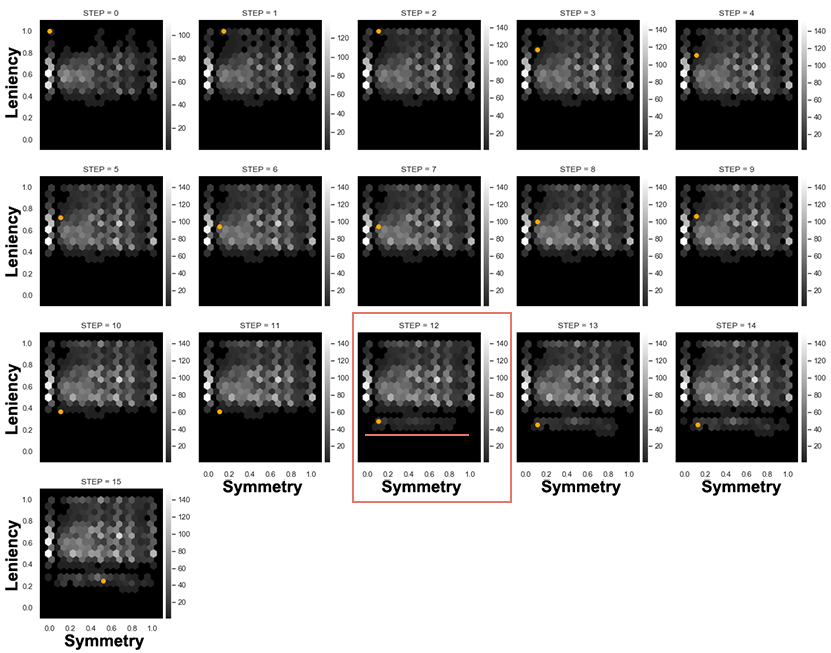
\includegraphics[width=\textwidth]{figures/ICMAPE-figs/accumulative__X-sym-Y-len-2.png}}
% %\centerline{\includegraphics[width=0.55\textwidth]{figures/low-len/accu__X-sym-Y-len.png}}
% \caption{Aggregated Expressive Range Analysis using Symmetry and Leniency as feature dimensions. The orange dot represents the designer's design that each step is edited and moving in the generative space. In step 12, it is highlighted the step when the designer's design enters a new generative area, which helps~\acrshort{icmape} explore the new area.}
% \label{fig:FigureRejectedPaper}
% \end{figure}

% Moreover, the work in \textsc{paper i, ii, ii} and the interest on seeking alternative approaches to foster creativity, to create adaptive experiences, and to enable more autonomy and initiative for the AI directed the research towards player and designer modeling. The former was explored in \textsc{paper iv}, where personality-driven player models were created to investigate their usability as a representative surrogate model and possible complement value in gameplay. 

% % Designer Modeling was explored through \textsc{paper v, vi}.
% \textsc{paper v} and~\textsc{paper vi} presented examples of designer modeling by modeling different designers' procedures. These could be used as surrogate models to enhance the understanding of design processes and the usability of design tools, such as~\acrshort{edd}. \textsc{paper v} presented a clear artifact design used to steer the generation of new suggestions based on the \textit{in situ} created preference model. This work demonstrated the benefits that come with integrating these models in the~\acrshort{mi} loop, such as the possibility of seamlessly creating preferred content. However, it also demonstrated the challenges of selecting and collecting representative data or training-and-using models as designers develop.

% Furthermore,~\textsc{paper vi} presented the development of a novel model to analyze the designer's design process, which could inform generative processes on the designer's style, goal, and intentions. The analysis of the resulting clusters based on each designer's design process resulted in the designer personas. These designer personas were presented as archetypical paths taken by designers through the clustered style space. Both models allow for the analysis of design and creative processes from an abstract level rather than specific steps, akin to procedural personas or game design patterns. 

% These approaches towards designer modeling have shown the capabilities of modeling several procedures and how they could be used. They also show that design processes can be analyzed more abstractly, yielding interesting similarities among seamlessly different designers or design processes. Designer modeling has the possibility to create adaptive experiences for an individual or group of designers and could enable more autonomy and initiative for the AI. However, whereas this, and its usability as surrogate models to enhance the collaboration, interaction, and generation produce actual benefits to the dynamic workflow of~\acrshort{micc} tools remain open for exploration as a promising area.

% If the aim of this research area is to push harder for mixed-initiative tools, where more autonomy is given to the AI, and for humans to consider the AI as a colleague as described by Lubart~\cite{LUBART2005-computerPartners} and Guzdial et al.~\cite{Guzdial2019-AISystemDesign-Creators} that can be taken serious and used its input as a key factor in the development of any type of content. Then we are required to develop AIs and tools that not only provides interesting and valuable input to the human, but also adaptive experiences that 

% \subsection{Future Work}

The work in this thesis had an ambitious overarching objective, which was partly explored, but that revealed many more exciting areas and paths to continue exploring.

% The work in this thesis explored MI-CC, its properties, and game design b

% \textsc{RQ1} was partly addressed by introducing and implementing~\acrshort{icmape} in~\acrshort{edd}, and exploring its use to generate different type of content, . However, it is necessary to examine the behavior of~\acrshort{icmape} when used for this interaction. These behaviors could be: how the generative space is affected by the design sessions, the combination with designer modeling, or how dynamic feature dimensions (e.g., similarity and inner similarity) affect the expressiveness of the algorithm.~\acrshort{pcg} through~\acrshort{qd} was proposed recently~\cite{gravina_procedural_2019}, pointing towards the interesting avenues that are approaching, and as discussed in this thesis, the many possibilities they have when introduced in human-AI interaction and collaboration.

% Furthermore, two approaches have been proposed to model different designer procedures as designer modeling, but more work needs to be in place to operationalize the findings and models. For instance, using and transforming the designer personas and the design style clustering presented in \textsc{paper vi} into an applicable model to study designers and their design and creative process. Moreover, how to use these models to steer the generation of content and create adaptive experiences remains open, as the interaction with designers is dynamic and heterogeneous.

\subsection{Human-AI Collaborative Properties}

This thesis has emphasized controllability as a core property in MI-CC systems that needs to be taken into consideration. We have argued that control can come at the expense of expressivity but with the aim of adaptability towards the designer. Using IC MAP-Elites, we have shown that not only expressivity does not need to be hindered by this, but that control can be a win-win situation for both the designer and the algorithm. However, these properties: ``controllability,'' ``expressivity,'' or ``adaptability,'' miss much of their nuance and their usability when taken as overarching properties. For instance, how can we calculate ``controllability'' or ``adaptability,'' and what would that mean? What would it mean to be 30\% percent adapted? These questions highlight the problem that these properties encompass too much meaning and require to be broken down and explored deeper. For instance, ``controllability'' could be explored on how control varies when this is direct or indirect; or when applied to the process, the product, or the other agents; or how it affects and changes the role of each agent. Exploring how these properties can be broken down and how to analyze systems with them to move towards deeper and more developed interactions and collaborations is an exciting open research area.

% Find those critical points where AI needs to (1) change role, (2) adapt, (3) take more control/agency/initiative. Basically identify designer's intentions.

% \begin{itemize}
%     \item Controllability
%     \item explainability
%     \item Adaptability
% \end{itemize}

\subsection{Designer Modeling and Adaptive Experiences}

%Find those critical points where AI needs to (1) change role, (2) adapt, (3) take more control/agency/initiative. Basically identify designer's intentions.

Two approaches have been proposed to model different designer procedures as designer modeling, but more work needs to be in place to operationalize the findings and models. For instance, using and transforming the designer personas and the design style clustering
presented in \textsc{paper ix} into an applicable model to study designers and their design and creative process. Moreover, how to use these models to steer the generation of content and create adaptive experiences remains open, as the interaction with designers is dynamic and heterogeneous.

Another interesting future work would be to use these adaptive models to identify and understand the designers' intentions. By knowing the designer's intentions and their current design process, one could adapt and tailor the system towards their needs. For instance, it would be important to find the critical points in the design process where AI could need to change role, adapt the generated content, or take more control, agency, or initiative.

%Adapting towards their intentions could help 

\subsection{Explainable AI}

To establish an in-depth relationship between human and AI, trustworthiness is also required from the AI, in order to give more autonomy, responsibility, and initiative to the AI in creative tasks. Explainable AI is a research field that aims at increasing the transparency of AI systems, making AI systems more accessible and more understandable~\cite{adadi_peeking_2018,doshi-velez_considerations_2018}.

Zhu et al.~\cite{zhu_explainable_2018} proposed the field of eXplainable AI for Designers (XAID) as a human-centered perspective on MI-CC tools. This work discusses three principles of mixed-initiative, \emph{explainability}, \emph{initiative}, and \emph{domain overlap}, where the latter focuses on the study of the overlapping creative tasks between game designers and black-box PCG systems in mixed-initiative contexts. Xie et al. present an example of this~\cite{xie_interactive_2019}, where they explored visualization techniques through an interactive level designer tool called \textit{QUBE} to explain and introduce machine learning principles to game designers.

% However, given the collaborative nature of the tasks and relation that human and AI have in these settings, there is the possibility that through Human-AI collaboration \emph{explainability} could be intrinsic to the collaboration. As humans explore and try different alternatives with these algorithms and models (e.g., virtual thinkering), better understanding and interpretation from how these models work could be achieved such as in~\cite{xie_interactive_2019}. Zhu et al.~\cite{zhu_player-ai_2021}

% Zhu et al.~\cite{zhu_player-ai_2021} explore connections between gameplay and AI-human interaction, arguing that “AI as play can expand current notions of human-AI interaction, which are predominantly productivity-based.” They suggest using play to help people discover capabilities of an AI-enabled tool.

% \textbf{Digital thinkering}

% \emph{Thinkering}, the idea of doing something with yuor hands 

\subsection{Holistic Procedural Content Generation}

In this thesis, we scratched the surface of holistic PCG and its implementation in MI-CC systems. Whole systems, where facets are not only intertwined, but designers can start the design process from any of them, is a very interesting path. If designers were able to start by designing quests or objectives, and the system could adapt to these and generate levels or structures to support these or vice versa, MI-CC tools would be more aligned with how design processes start. These do not often start from the same starting point but tend to vary, and allowing that variance might be necessary to have different and more fruitful creative experiences. The system would then be in accordance with both Dehn’s definition, that space (world) is developed as post hoc justification for events by authors~\cite{dehn_story_1981}, and with Lebowitz, that the story gives meaning to a created world~\cite{lebowitz_creating_1983}. 

% An interesting and exciting path would be to explore the concept of holistic~\acrshort{pcg} and orchestration of the different game facets~\cite{liapis_orchestrating_2019} in connection with the~\acrshort{mi} paradigm. Holistic~\acrshort{pcg} is the generation of multiple contents (in different game facets) fitting each other in harmony as a collaborative process akin to how games are developed, with a limited amount of examples, but exhibiting exciting results~\cite{hartsook_toward_2011,cook_rogue_2014,hoover_audioinspace_2015,smith_situating_2011,dormans_generating_2011}. However, to what extent the generation is created in such a harmony that the facets interact and affect each other, and to what degree the user can interact with it is an open area for active research. 

% Furthermore, there exists an essential link and relation between space (e.g., level or objects within) and narrative (e.g., the story tried to be told). Thus, choosing and associating level design and narrative as two facets to explore within the holistic~\acrshort{pcg} approach is appropriated. This was presented and described by Kybartas and Bidarra's survey~\cite{kybartas_quinn_survey_2017}, and explored and supported by related work~\cite{kishino_hunt_2005,dehn_story_1981,lebowitz_creating_1983,hartsook_toward_2011,karavolos_mixed-initiative_2015,abuzuraiq_taksim_2019}. Within the narrative facet and in most games, quests are an essential component. Therefore, exploring and generating quests is paramount by exploring multiple quest concepts~\cite{yu_what_2020}, analyzing quest patterns~\cite{trenton_quest_2010,smith_situating_2011}, and using surrounding ideas such as kernels and satellites for event division~\cite{aarseth_narrative_2012}.


%using different denifitions~\cite{yu2020quest}, Within the narrative facet as well as in most games, quests are an essential componen I want to add this work by Yu et al.~\cite{yu2020quest}

% It is paramount to identify the roles, goals, conflicts, relations that exist in a narrative scenario 
%Quests have been studied 

% Thus far, some exploratory work has been done combining both facets in the generative process of~\acrshort{edd}. Firstly, through a simple but effective way of analyzing patterns and objectives created by designers when designing their levels~\cite{flodhag_make_2020}. Secondly, by introducing~\acrshort{mi} creation of quests using grammars based on the quest analysis by Doran and Parberry~\cite{doran_prototype_2011}, to compose a series of subsequent objectives together with the designer~\cite{alvarez_questgram_2021}. 

% Therefore, having this as a base and using the current findings in this thesis, the aim is to explore the~\acrshort{micc} paradigm applied to holistic~\acrshort{pcg} through the following RQ and subRQs (continuing the numbering from the RQs presented in this thesis): 

% \begin{itemize}
%     \item[] \textbf{RQ4.} How can level design and narrative interact, act as constraints, be intertwined, and in general, have an active role affecting each other, in order to, produce a holistic system?
%     \begin{itemize}
%         \item[] \textbf{RQ4.1:} What are the requirements and main factors needed to establish a relation between the level design and the narrative, and what are the criteria to evaluate the respective generated content? 
%         \item[] \textbf{RQ4.2:} What are the factors to be considered when implementing such a paradigm and system in a mixed-initiative application, where a designer will be able to interact with the content?
%         \item[] \textbf{RQ4.3:} What are the effects of producing and using a holistic system for the creative process of a designer, and what challenges are imposed on computational creativity? 
%     \end{itemize}
% \end{itemize}


\subsection{Exploring Agency and Initiative in Mixed-Initiative}

As paths towards adaptive experiences that recognize several designer procedures are explored, it is expected to establish the foundations of a deeper relationship between humans and AI. Through this thesis, control mechanisms were given to designers while not reducing the expressiveness of the AI. Further, examining and modeling different designer procedures, such as their design process, style, preferences, and goals as they create content, have enabled this thesis to explore important steps towards a mature relationship. It is hypothesized that this is needed to create more autonomy and initiative for the AI and to establish a trustworthy relationship between both agents, yet, this might not be enough. This thesis barely scratched the surface of the relationship, the possibilities that emerge with them, and the AI's initiative and role. In \textsc{paper xii}, we took the first steps toward altering the role and agency of both humans and AI, and had interesting results that still require much exploration. Therefore, another future direction is to explore varying autonomy, agency, and initiative for both agents and how that affects the interaction and design and creative process of the co-design and~\acrshort{mi} paradigm.

% This is compiled into the following RQ:


% is how varying the autonomy, agency, and initiative of t

% \begin{itemize}
%     \item[] \textbf{RQ5.} How does the agency of the designer and the agency of the computational designer in mixed-initiative approaches, and the interaction between both actors, affects the overall design process and the usefulness of mixed-initiative tools?
% \end{itemize}

% \subsubsection{Different Interactions}

% Finally, it is exciting to have explored all that this thesis present, but it is even more to see the road in front and realize all the paths that remain open and to be explored through future work.


% while this thesis has presented steps towards a better understanding through designer modeling and , it is especulated this thesis only especulates  has explored speculates that both of these research areas are needed to establish a trust relationship between both actors, yet, this might not be enough.

% Giving control to the designer while not reducing the expressive power of the AI, understanding different designer procedures such as their design process, style, and goals as they create levels, and modeling multiple subjective properties such as designers preferences and intentions; have enabled this thesis to explore interesting and important steps towards a mature relation. However, this thesis barely scratched the surface of the relationship and the possibilities that emerge with them. 

% Moreover, as it is explore paths towards adaptive experiences that recognize several designer procedures; we hope to establish the foundations of a deeper relation between human and AI. Giving control to the designer while not reducing the expressive power of the AI, understanding different designer procedures such as their design process, style, and goals as they create levels, and modeling multiple subjective properties such as designers preferences and intentions; have enabled this thesis to explore interesting and important steps towards a mature relation. However, this thesis barely scratched the surface of the relationship and the possibilities that emerge with them. 

% Moreover, as introduced in the problem statement (see section~\ref{sec:problemst}), it is required to have both an understanding from the AI of the multiple human procedures and an understanding from the human of how the AI system operates and it's decision process. In this thesis, this has been used and explained as Designer Modeling~\cite{Liapis2013-designerModel} and Explainable AI~\cite{Zhu2018-XAIDesignersMICC}. However, while this thesis has presented steps towards a better understanding through designer modeling, it is especulated this thesis only especulates  has explored speculates that both of these research areas are needed to establish a trust relationship between both actors, yet, this might not be enough. There are 


% As introduced in the problem statement (see section~\ref{sec:problemst}), it is required to have both an understanding from the AI of the multiple human procedures and an understanding from the human of how the AI system operates and it's decision process,  which translates to Designer Modeling~\cite{Liapis2013-designerModel} and Explainable AI~\cite{Zhu2018-XAIDesignersMICC}. However, such a system does not exist, and this thesis speculates that both of these research areas are needed to establish a trust relationship between both actors, yet, this might not be enough. There are 

% \begin{itemize}
%     \item[] \textbf{RQ5.} How does the agency of the designer and the agency of the computational designer in mixed-initiative approaches, and the interaction between both actors, affects the overall design process and the usefulness of mixed-initiative tools?
% \end{itemize}

% It is exciting to have explored all this thesis present, but it is even more to see the road in front and realize all the paths that remain open and to be explored through future work.



\let\oldthebibliography=\thebibliography
\renewenvironment{thebibliography}[1]{%
   \oldthebibliography{#1}%
   \setcounter{enumiv}{0}%
}


% \bibliographystyle{ieeetr}
\bibliographystyle{ieeetr}
\phantomsection
\addcontentsline{toc}{section}{REFERENCES}
\bibliography{references-zot,methodologies,games}
% % \bibliographystyle{apalike}
% \nobibliography{publications}


\setcounter{secnumdepth}{1}

\cleardoublepage
\part{PAPERS}
\clearpage

\setcounter{secnumdepth}{-30}

% \renewcommand\thefigure{\thesection.\arabic{figure}}  
\setcounter{figure}{0}    
\setcounter{equation}{0}
\setcounter{table}{0}    
\setcounter{footnote}{0}    
\setcounter{enumi}{0}
\setcounter{enumii}{0}
\setcounter{enumiii}{0}
\setcounter{enumiv}{0}

% \clearpage


\includedPaper{\textsc{paper i - fostering creativity in the mixed-initiative evolutionary dungeon designer}}{Paper I - Fostering Creativity in the Mixed-Initiative Evolutionary Dungeon Designer}{Alberto Alvarez, Steve Dahlskog, Jose Font, Johan Holmberg, Chelsi Nolasco, and Axel Österman}

% \section{\textsc{paper i - fostering creativity in the mixed-initiative evolutionary dungeon designer}}

% \vspace{-10pt}
% \textit{Alberto Alvarez, Steve Dahlskog, Jose Font, Johan Holmberg, Chelsi Nolasco, and Axel Österman}

\normalfont
\textbf{\textsc{ABSTRACT}}

Mixed-initiative systems highlight the collaboration between humans and computers in fostering the generation of more interesting content in game design. In light of the ever-increasing cost of game development, providing mixed-initiative tools can not only significantly reduce the cost but also encourage more creativity amongst game designers. The Evolutionary Dungeon Designer (EDD) is a mixed-initia-tive tool with a focus on using evolutionary computation to procedurally generate content that adhere to game design patterns. As part of an ongoing project, feedback from a user study on EDD's capabilities as a mixed-initiative design tool pointed out the need for improvement on the tool's functionalities.

In this paper we present a review of the principles of the mixed-initiative model, as well as the existing approaches that implement it. The outcome of this analysis allows us to address the appointed needs for improvement by shaping a new version of EDD that we describe here. Finally, we also present the results from a user study carried out with professional game developers, in order to assess EDD's new functionalities. Results show an overall positive evaluation of the tool's intuitiveness and capabilities for empowering game developers' creative skills during the design process of dungeons for adventure games. They also allow us to identify upcoming challenges pattern-based mixed-initiative tools could benefit from.

\textbf{\textsc{PUBLISHED IN}}

Proceedings of the 13th International Conference on the Foundations of Digital Games, ACM, 2018

\section*{FOSTERING CREATIVITY IN THE MIXED-INITIATIVE EVOLUTIONARY DUNGEON DESIGNER}

\subsection{Introduction} 

Mixed-initiative systems in game content creation~\citepone{p1shaker_procedural_2016} refer to the combination of functions produced by procedural content generation (PCG) algorithms and human designer intentions. 

In today's design paradigm, it is a common approach to have humans and machines collaborate to maximize creativity during the design process and thus software have become a backbone tool for a designer to create artifacts within the areas of architecture, consumer product and interior design. As a result, computer-aided design (CAD) has been an important facet for design practices~\citepone{p1yannakakis_mixed-initiative_2014}. It could be argued that game development is a fast growing application area for this facet.

Games are part of an evolving medium of creative expression, but limitations still exist in regards to its design tools’ accessibility due to the fast paced life cycle and expensive nature of game development. The rising cost in game development due to games’ technological evolution has resulted in a push towards automatically generated content ~\citepone{p1yannakakis2018artificial,p1font_constrained_2016,p1Doherty2005-ji}. Cost drivers may include multiple factors, but in the context of work processes involving human designers and artists, they are commonly identified as a huge contributor, since they are expensive. Games' complexity in design, requires the involvement of tens to hundreds of staff across a development period that may span for years. This can negatively affect a company’s profitability and the development team’s innovative and creative vision. 

PCG approaches and functionalities are used to reduce the workload of developers, and to promote cooperation between humans and machines by providing more diverse game content that could increase quality and re-playability ~\citepone{p1liapis_generating_2013,p1yannakakis2018artificial}. Various development tools and level editors can be used by human designers at their disposal, making them the sole driver of the creative process. 

PCG, however, may limit the human designer’s intentions by strictly following its own algorithms, disregarding the designer’s desired parameters before generation~\citepone{p1yannakakis_mixed-initiative_2014}. Rather than simply being limited tools of support for the other, mixed-initiative systems can foster co-creativity in game design by combining the best of these two perspectives. Not only would it improve a development team’s overall productivity, it can also guide and improve the creativity of smaller indie teams and individuals in developing more interesting and content-rich games with less worries about development costs~\citepone{p1MachadoCiceroSeekWhence,p1liapis_generating_2013}. 

This paper is organized as follows: Section~\nameref{p1background} presents the related work in Mixed-Initiative design and the previous results of Evolutionary Dungeon Designer, both of them as motivation for the current work. Section~\nameref{p1approach} describes the contributions of this paper together with a description of the last release of the tool. Section~\nameref{p1userstudy} presents the results from the user study conducted with game developers, followed by the conclusions and future work discussed in Section~\nameref{p1conclusion}.

\subsection{Related work} \label{p1background}
\subsubsection{The Main Principles of Mixed-Initiative}

There are two different types of mixed-initiative~\citepone{p1shaker_procedural_2016}. The first type relates to the human creator having an idea and the computer being the mean of expression through aiding the human in their creative task (e.g. a text editor or Photoshop). The second type is described as the computer autonomously generating content and being evaluated, changed and edited by a human designer. This division is also described by \citepone{p1yannakakis2018artificial} where they present a scale with the two extremes on opposite ends: purely human design on one and purely computational design on the other. In between these extremes are varying forms applied to mixed-initiative content generation tools used for game design. 

Artificial intelligence (AI) techniques have become more common and essential on aiding designers while they develop games~\citepone{p1togeliuspanorama}. This motivates the use of mixed-initiative systems, which promotes the co-creativity between human designers and machines providing more interesting and exciting creations~\citepone{p1yannakakis_mixed-initiative_2014}. However, there are still some problems when generating content, thus advocating developers still doing manual designs from scratch. Some drawbacks of completely relying on PCG is the low reliability, believability, and high predictability of the game content - all which guarantees difficulties in evaluating the generated content like, for instance, a dungeon level's quality~\citepone{p1karavolos_mixed-initiative_2015}. Therefore, by following the principles of mixed-initiative through combining the content generation with the guidance and input from a human designer, you provide aspects from both parties, hopefully limiting the weaknesses from either.  

\subsubsection{Mixed-Initiative Tools in Game Design}

Recent research in the field has presented different approaches to mixed-initiative authoring tool. These are \emph{Tanagra}, \emph{CICERO} and the \emph{Sentient Sketchbook}. While all these provide mixed-initiative interfaces to the designer, they also share the limitation of addressing a specific game type. 

\emph{Sentient Sketchbook} aims at generating maps for strategy games such as \emph{Starcraft}~\citepone{p1liapis_sentient_2013}. Users can sketch a low-resolution map that seeds an underlying evolutionary algorithm that provides suggestions. Low-resolution sketches reduce the creative strain on the user during the design process, but also makes it easier for the program to detect patterns in the map. Once the user deems the generated and edited low-resolution map good enough, the program can then generate the higher resolution map while still maintaining the patterns that were detected in the sketch. 

\emph{Tanagra} is used to develop 2D platformer levels~\citepone{p1Tanagra2011}, while still checking whether the generated content is playable or not. Tanagra offers users an empty grid where they can place different tiles such as floor, enemies, and coins. Mixed-initiative is implemented so that users can select tiles and objects they want to keep in their designs, while Tanagra generates new content around them. 

\emph{CICERO} focuses on the generation of dungeons for adventure games~\citepone{p1MachadoCiceroSeekWhence}. CICERO offers users the possibility to define the behavior of the game components they include in their designs, such as power-ups, win and lose conditions, and collision-triggered behavior. From these definitions CICERO recommends different game mechanics that would suit the game, such as the optimal weapon types to include in the game. By manually editing game content in the dungeon and having CICERO run the game and test different element combinations, users can understand how different layouts affect the generated gameplay. 

\subsubsection{Dungeon Design in Videogames}
The dungeon is a popular level design archetype found in several popular game genres~\citepone{p1miyamoto_legend_1986,p1brevik_diablo_1996}. Dungeons are also popular in PCG research, where different approaches have been presented for generating dungeon levels~\citepone{p1shaker_procedural_2016,p1johnson_cellular_2010,p1dormans_adventures_2010,p1van_der_linden_designing_2013,p1karavolos_evolving_2016}. These works emphasize the importance of considering goals, missions, the narrative or themes, visual style, and gameplay rules when designing levels, therefore they should be taken into consideration when developing a mixed-initiative tool for content generation~\citepone{p1karavolos_mixed-initiative_2015}. These factors are mostly decided by the human designer, thus a designer has to be integrated into the dungeon generation process. 

Another key aspect to dungeon generation is player progression~\citepone{p1butler2013mixed}. Designers ensure that the player’s experience throughout a level will be coherent and effective, which will be affected by the content they create. This includes reward and challenge balancing among the rooms in a dungeon.

\subsubsection{The Evolutionary Dungeon Designer}

\begin{figure}[t]
    \centering
    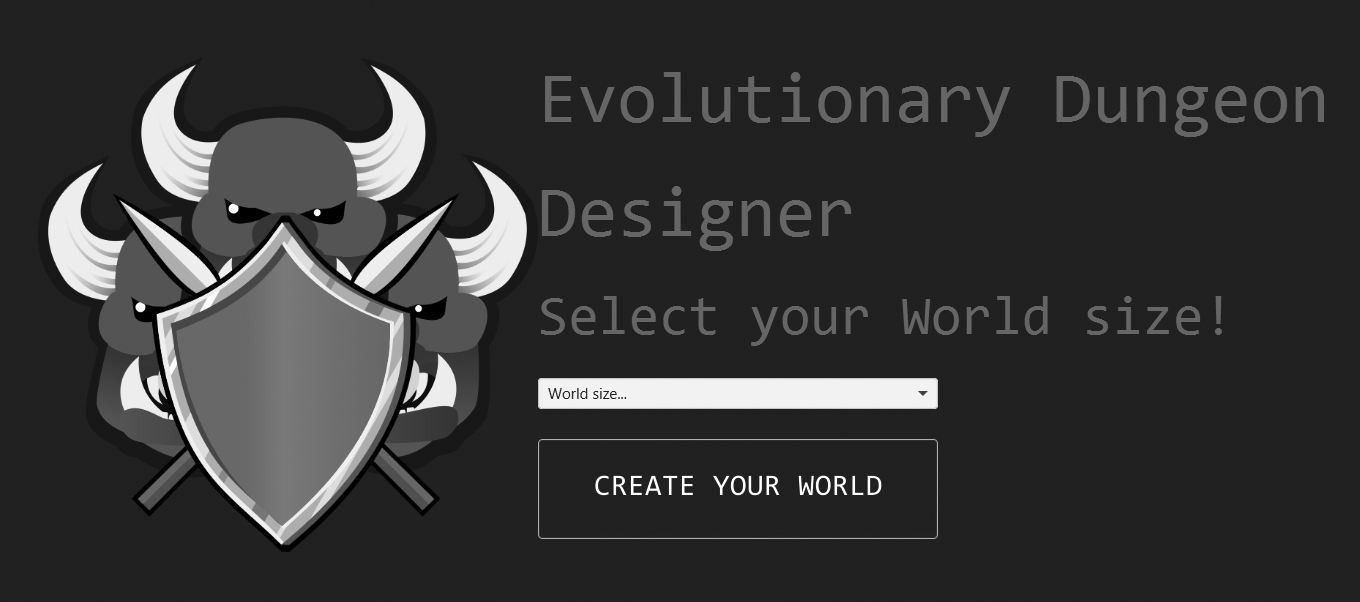
\includegraphics[width=1\columnwidth]{included-papers-tex/paper-1/figures-extra/start-edited.png}
    \caption{The start screen lets users choose the dungeon dimensions.}~\label{p1fig:launch}
\end{figure}

Previous research presented the \emph{Evolutionary Dungeon Designer} (EDD)~\citepone{p1Eddy1_5, p1Eddy2} as a mixed-initiative authoring tool for designing dungeon rooms for adventure games. EDD automatically generates and suggests rooms to the user while the user is manually designing one of them. The user either form the room from scratch or from a previously generated suggestion. This is done by means of a FI-2Pop GA~\citepone{p1kimbrough_feasibleinfeasible_2008}, where game design patterns are used both as input parameters and as objectives. These patterns involve micro-patterns (\textsc{Enemy}, \textsc{Treasure}, \textsc{Chamber}, \textsc{Corridor}, \textsc{Connector}, \textsc{Entrance}, and \textsc{Door}) as well as meso-patterns (\textsc{Ambush}, \textsc{Guard Chamber}, \textsc{Treasure Chamber}, and \textsc{Guarded Treasure}). EDD also ensures that all generated rooms are playable.

Initial experiments on EDD~\citepone{p1Eddy1_5} validated its PCG system in terms of fitness optimization, pattern detection, and solution diversity, providing a sufficient level of control to the designer. The following iteration~\citepone{p1Eddy2} explored the capabilities of EDD as a mixed-initiative level generator as a means of facilitating collaboration between human designers and PCG algorithms. Among its key features, the participants of a user study highlighted EDD as a useful framework for working with game design patterns in the context of search-based problems. The suggestions were considered a good source of inspiration as well as time saving. This user study also shaped the roadmap for future improvements on EDD. This included extending EDD from room generation to complete dungeon generation, and preserving the users' designs to a higher degree in relation to both design patterns and room aesthetics.

This version of EDD extends previous work based on the aforementioned user study by implementing the following key improvements:

\begin{itemize}
  \item The designer is now able to construct, develop, and edit a grid-based dungeon of different dimensions and inter-connected rooms, in contrast to a single room, which in turn, helps the designer on having context over their work on individual rooms and giving them more freedom on producing variations.
  \item The designer receives extended information about the consequences of their changes in individual rooms, and the differences between the current edited room and the proposed suggestions by the EA.
  \item The UI has been renovated to account for the newly added features by means of different views and options, as well as, a better structure and distribution of the different elements in the generator.
  \item Navigation tools have been added within a view and between views, which provides an overview of the dungeon, along with a better context of the edited room.
  \item The EA has been updated to assess and preserve the aesthetic criteria of the designer by means of a new capability of locking sections of an edited room for preserving custom aesthetic structures, and by extending the evaluation function through the measurement of symmetry and similarity in the provided suggestions, both which are further explained in \citepone{p1Eddy2_5}.
\end{itemize}

\subsection{Improving the Mixed-Initiative Evolutionary Dungeon Designer} \label{p1approach}

\cref{p1fig:launch} shows the start screen in EDD, which starts a new workflow by prompting users to choose the maximum number of rooms in the dungeon to be developed. The dimensions range from 2x2 rooms up to 7x7 rooms in a square dungeon grid (also referred as world grid). From this point, the workflow offers users three different views: 1) a world view for dealing with aspects regarding the dungeon as a whole; 2) a room view which places the focus in a particular room in the dungeon; and 3) the suggestions view, which produces six different suggestions with diverging room configurations (e.g. more corridors or more chambers) for the user to choose from. The user can freely alternate between views during the design process. The current dungeon layout can be saved at any moment from either of the views.

\begin{figure}[t]
    \centering
    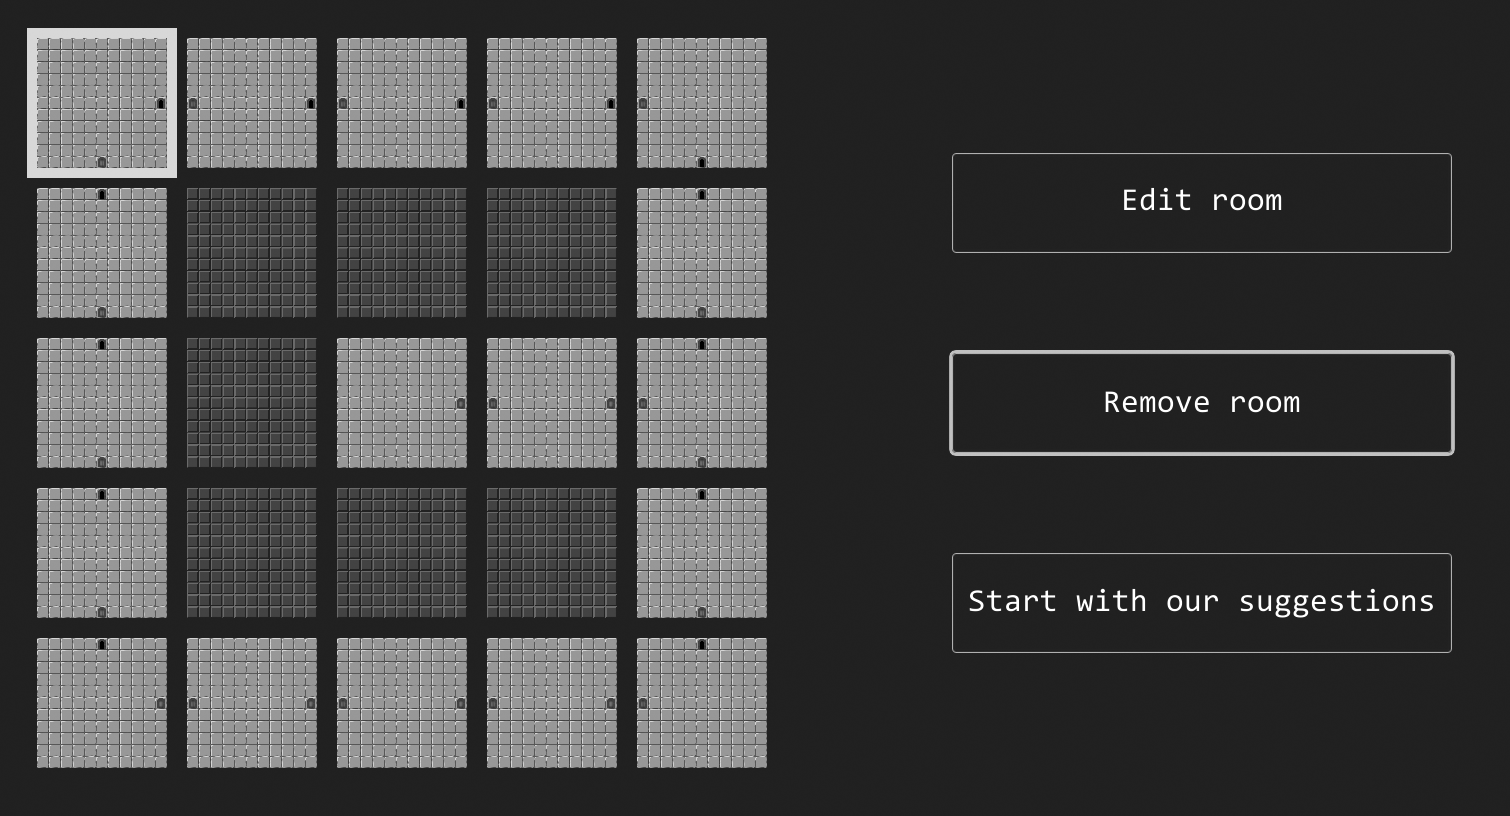
\includegraphics[width=\columnwidth]{included-papers-tex/paper-1/figures-extra/world-edited.png}
    \caption{Sample world view showing a 5x5 dungeon with 7 disabled rooms. User actions are displayed in the rightmost buttons.}~\label{p1fig:world}
\end{figure}

The world view (\cref{p1fig:world}) opens up right after the start screen, displaying a grid of the selected size composed by a fully connected set of empty rooms (all rooms are connected to their neighbors). The users can load a previously saved dungeon design, skipping the start screen and resume work from the state in which the dungeon design was saved.

From the world view users can then click and select any room to:
\begin{itemize}
\item disable or enable the room. Disabling makes the room inaccessible, removing all doors from the adjacent rooms. This can be undone by clicking \emph{enable}. Single rooms that become isolated after all their neighbors have been disabled, are automatically disabled as well. \cref{p1fig:dungeon1,p1fig:dungeon2} show two examples of dungeons with several disabled rooms,
\item get procedurally generated suggestions for that room in the suggestions view,
\item load the room in the room view for manual editing.
\end{itemize}

\begin{figure}[!ht]
    \centering
     \subfloat[\label{p1fig:dungeon1}]{%
       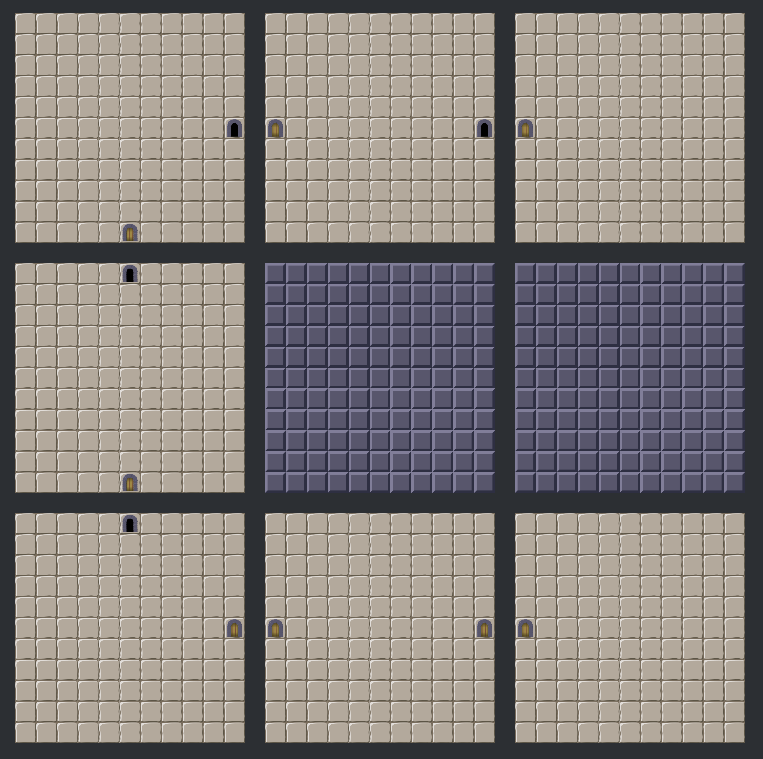
\includegraphics[width=0.49\textwidth]{included-papers-tex/paper-1/pap1-Figures/dungeon1.png}
     }
     \hfill
     \subfloat[\label{p1fig:dungeon2}]{%
       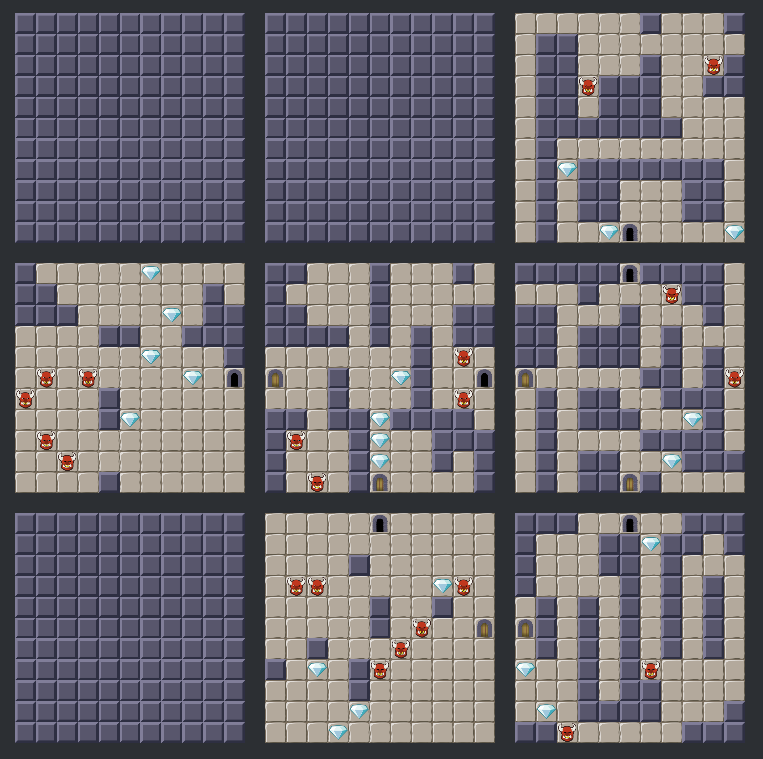
\includegraphics[width=0.49\textwidth]{included-papers-tex/paper-1/pap1-Figures/dungeon3-edited.png}
     }
    
    \caption{(a) 3x3 dungeon with 2 disabled rooms and 7 empty rooms, and (b) 3x3 dungeon completed dungeon with 3 disabled rooms.}
    \label{p1fig:dungeonsp1}
\end{figure}

\subsubsection{The Suggestions View}

By selecting ``Start with our suggestions'' in the world view (\cref{p1fig:world}) six uniquely generated rooms are presented to the user in a separate window: the suggestions view (\cref{p1fig:suggestionsview}). When clicking any of the suggestions, it will replace the previously selected room in the dungeon.

\begin{figure}[!ht]
    \centering
    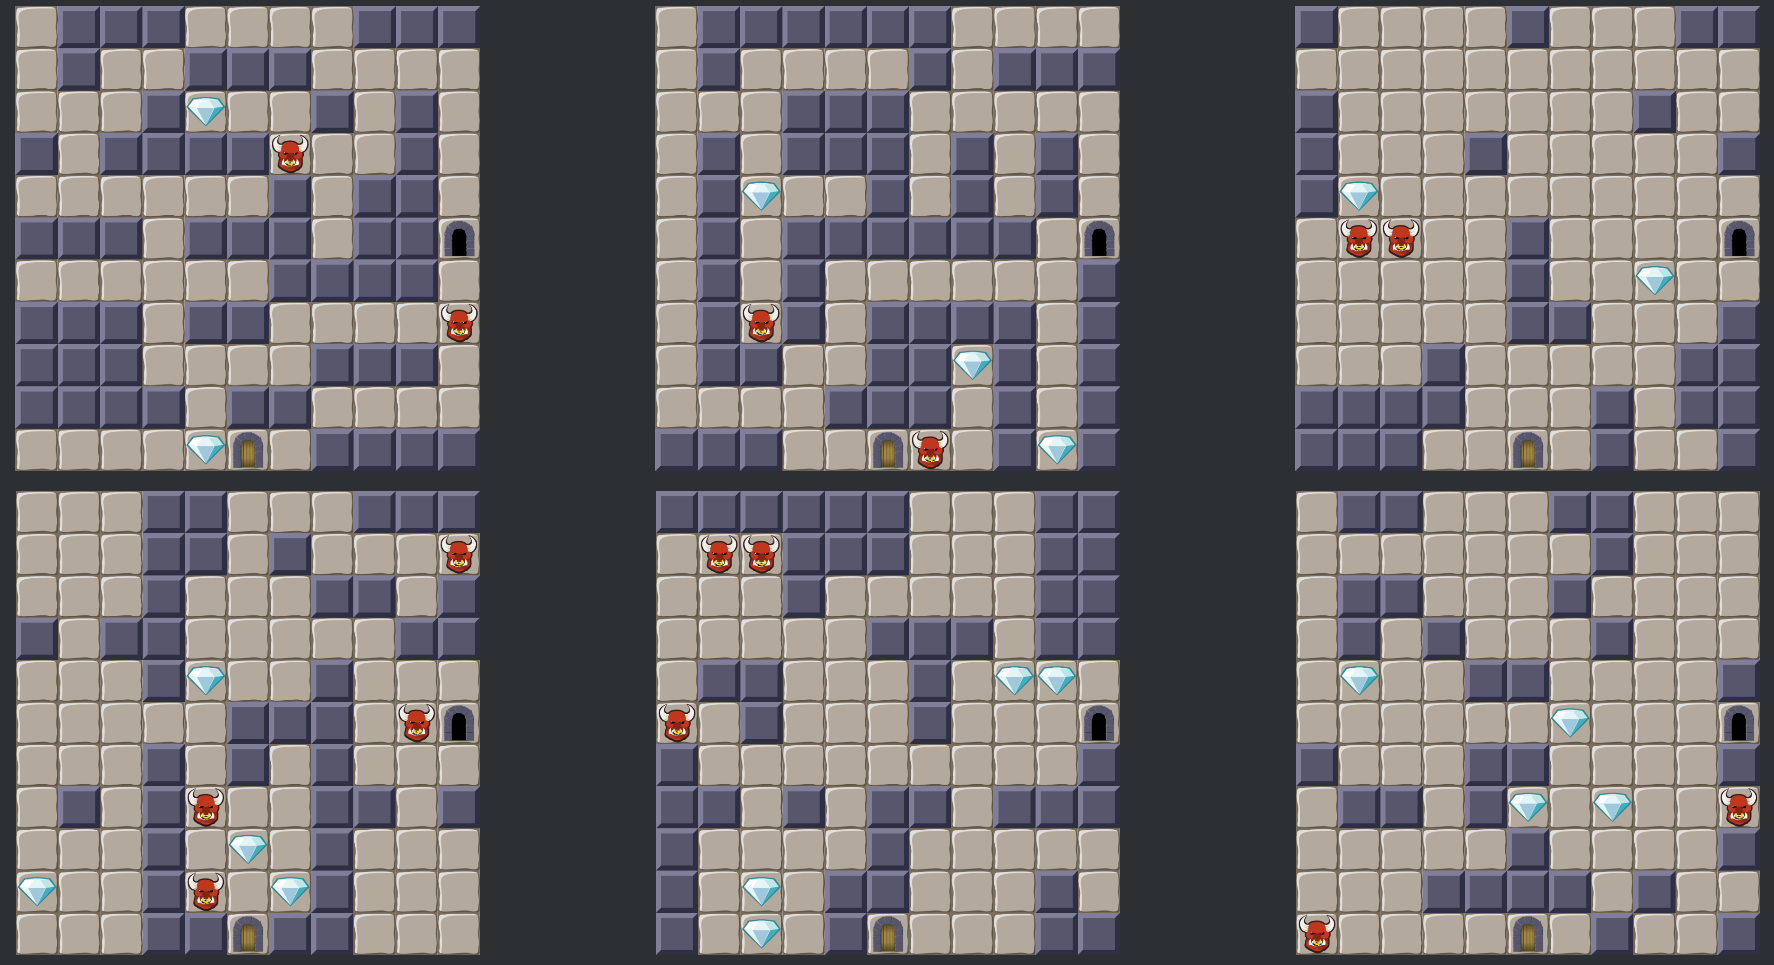
\includegraphics[width=\columnwidth]{included-papers-tex/paper-1/pap1-Figures/suggestionsview.png}
    \caption{Six procedurally generated rooms presented to the user in the suggestions view.}~\label{p1fig:suggestionsview}
\end{figure}

A similar functionality was present in the former version of the tool, presented only once as the start screen. Now users can freely alternate between the world and the suggestions views, getting as many suggestions as they need, deciding whether to start creating every room from a clean state or to get inspiration from one of the generated rooms.

\begin{figure*}[t]
    \centering
    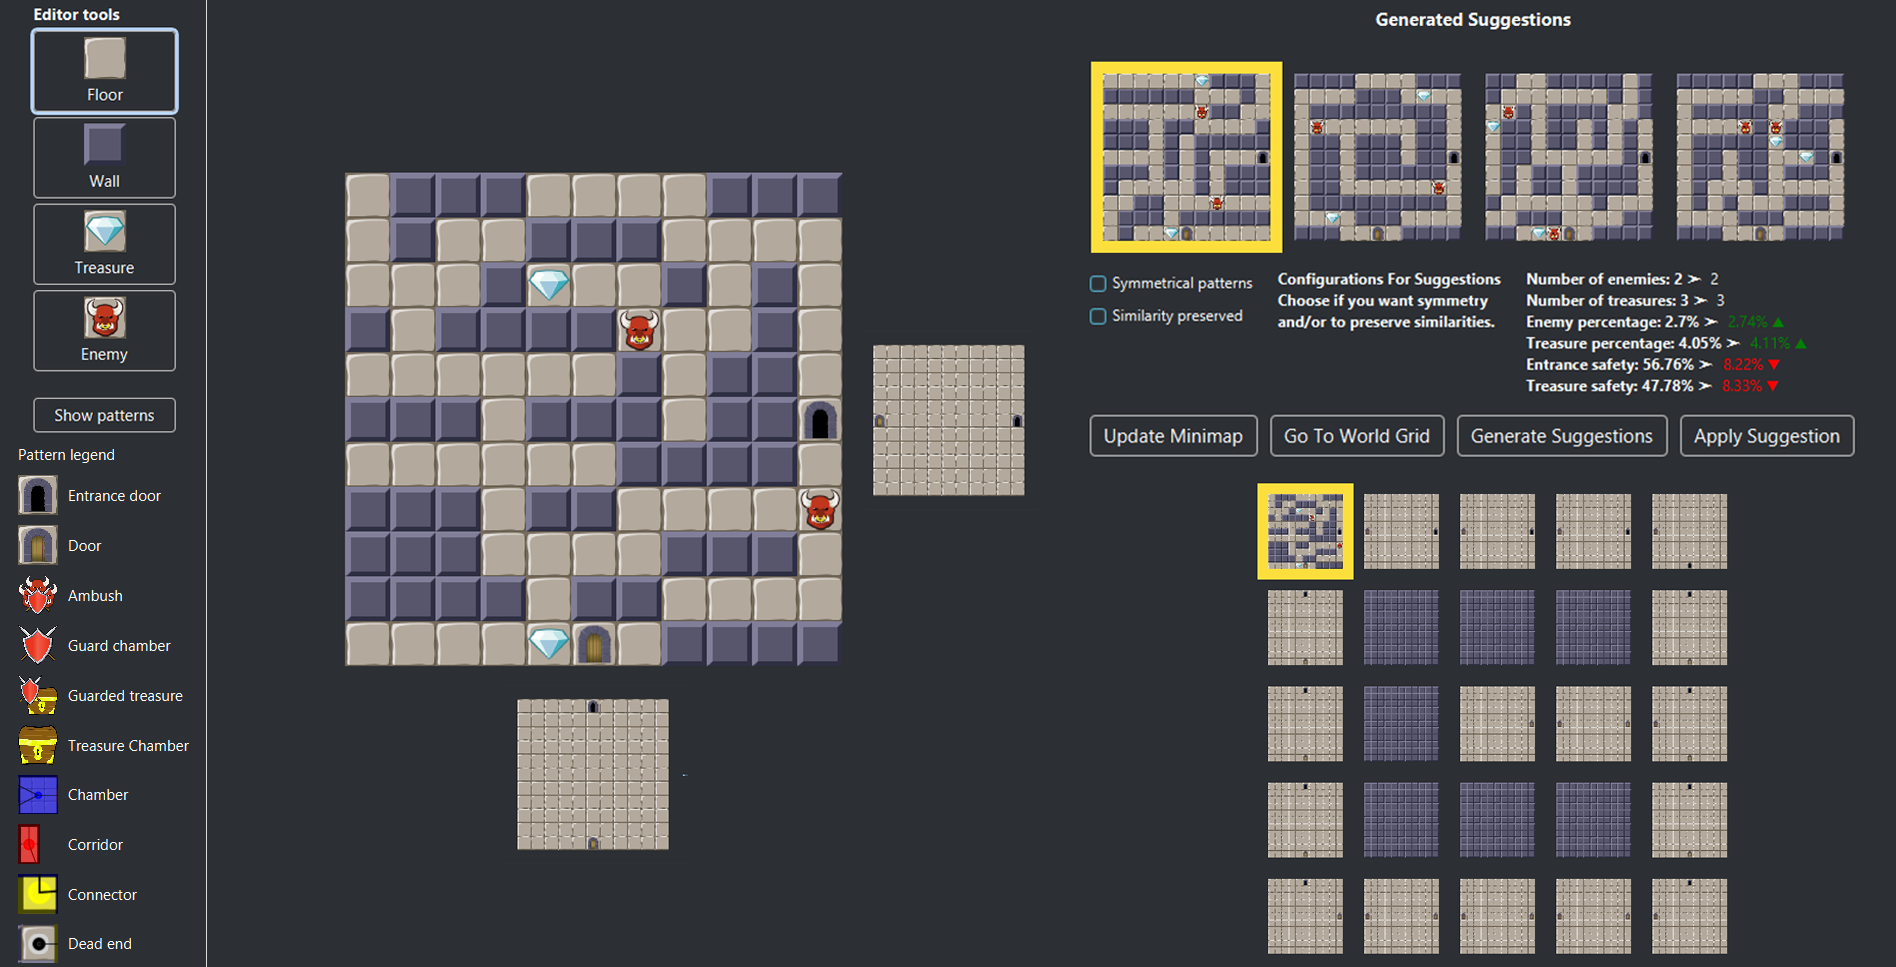
\includegraphics[width=\textwidth]{included-papers-tex/paper-1/pap1-Figures/roomview.png}
    \caption{The room view while editing the top-left corner in a 5x5 dungeon with seven disabled rooms.}~\label{p1fig:roomview}
\end{figure*}

Suggestions preserve the door layout from the room that was selected in the world view. The suggestions shown in \cref{p1fig:suggestionsview} have been created for the room selected in \cref{p1fig:world}, placed in the top-left corner, and containing only two doors connecting them to their east and south neighbor.

\subsubsection{The Room View}

\begin{table*}[ht]
% \centering
\caption{General consensus on EDD's features} \label{p1tab:consensus}
\resizebox{0.8\textwidth}{!}{
\begin{tabularx}{\textwidth}{|p{0.2\textwidth}|p{0.99\textwidth}|}
\cline{1-2}

Description & Participants’ Consensus \\\cline{1-2}
World Grid  of the dungeon                   & Its purpose of establishing an illusion of a fully realized dungeon is somewhat achieved. However, limitations exist with how it defines feasibility, a dungeon’s starting point, and the entrances, which disrupts the designers’ decisions.                                                                                                                                                                                   \\\cline{1-2}
World View                                  & The world view’s usefulness for the most part could not be established, other than for the purpose of going to the suggestions view (which was already seldom during the user study) and having a closer look at the entire dungeon without any distractions. Some participants preferred features to be already in the room view’s minimap, and some wanted to see more specific functionalities within the world view itself. \\\cline{1-2}

Enabling and  \newline disabling rooms                & As the user study restricted participants to create 3x3 dungeons, this feature for the most part has been neglected. This is also in part because of its accessibility only being in the world view, which proved to be an inefficient view in general. However, its use for bigger dungeon sizes later on was appreciated, especially for more intricate design purposes.                                                      \\\cline{1-2}
Suggestions View                            & Similarly to enabling and disabling rooms, it was quite difficult to encourage the use of this functionality due to the world view’s inefficient usability. However, this could also be due to the dungeon’s small size, as some participants expressed high interest in using more suggestions with larger dungeon sizes.                                                                                                      \\\cline{1-2}
Minimap  \newline  navigation                      & The minimap proved to be a strong tool not only for navigation purposes, but also for supporting design decisions and choices. The directional buttons were rarely used, but their room previews were helpful in emphasizing the current room’s connection to adjacent rooms without looking at the minimap. On the other hand, this lowered the usability of the world view.                                                   \\\cline{1-2}
Parameters                                       & The parameters were, in general, lacking. They served to be important in decision-making when choosing a suggested map in room view, but there were still doubts on their accuracy and sufficiency when providing information about the generated suggestions.                                                                                                                                                                       \\\cline{1-2}
Generated maps for  \newline  suggestions in room view & Suggestions in the room view proved to be very helpful in supporting the whole design process as they primarily acted as inspirations for the users. The most prominent comment among the users is the preference of having more control on how suggestions should be generated depending on different types of parameters.                                                                                                     \\\cline{1-2}
Design \newline  patterns& The patterns’ visualization was, in general, lacking and not self-explanatory. Some participants have expressed interest in using patterns as a parameter in the generation of suggestions.                                                                                                                                                                                                                                     \\\cline{1-2}
Dark theme                                  & EDD’s dark theme for the user interface received a positive response as it makes working with the program easier.
	\\ \cline{1-2}
\end{tabularx}
}
\end{table*}

% \begin{table}
% \begin{center}
% {\caption{Best performing setups based on their internal validation and visualization of clustered data points.}\label{table:setups}}
% \resizebox{\textwidth}{!}{
% \begin{tabular}{ccccccc}
% \hline
% \rule{0pt}{12pt}
% Algorithm&Data&K&$\Diamond$&$\Box$&$\bigtriangleup$ 
% \\ 
% \hline
% \\[-6pt]
% K-Means & Tiles-PCA & 9 & 0.43 & 0.73 & 9438.233 \\ 
% K-Means & Tiles-PCA & 12 & 0.41 & 0.77 & 9436.928 \\
% K-Means & Dimensions-PCA & 12 & 0.43 & 0.73 & 7738.343 \\
% Agglomerative single & Combined-PCA & 6 & 0.51 & 0.43  & 38.833 \\ 
% Agglomerative avg. & Dimensions-PCA & 6 & 0.44 & 0.67 & 3463.567 \\ 
% \hline
% \\[-6pt]
% \multicolumn{6}{l}{$\Diamond$ Silhouette Score\ \
% $\Box$ Davies Bouldin Index\ \
% $\bigtriangleup$ Calinski-Harabasz Index}
% \end{tabular}
% }\end{center}
% \end{table}

Users edit single rooms in the room view (\cref{p1fig:roomview}), regardless of whether these are new empty rooms, procedurally generated suggestions, or previously edited rooms. The room view is an improved and extended version of the main screen in the last version of EDD~\citepone{p1Eddy2}. All functionalities from that version are still present: manually editing the room by changing tiles (floor, wall, enemy, and treasure), displaying an overlay view of the existing design patterns, and procedurally generating suggestions based on the current edited room's configuration.

Navigation is one of the crucial added features, allowing users to move around the dungeon without going back to the world view. Two other options offer navigation through the dungeon: the navigational buttons and the minimap. The navigational buttons are displayed next to each of the edited rooms' borders that contain a door. Provided that the room being edited in \cref{p1fig:roomview} is located in the top-left corner, two navigational buttons are displayed right and below the room, respectively. Clicking a navigational button transports the user to that room, replacing the currently edited room with the targeted neighbor. Instead of using arrows or any other fixed picture, these buttons preview the neighboring rooms as a hint for users to help them design the room currently being edited. The navigational buttons are automatically refreshed to reflect up-to-date changes performed to the neighboring rooms.  

The minimap displays a scaled-down overall picture of the whole dungeon, highlighting the currently edited room with a yellow border. Users can navigate to any room, which is not disabled and is displayed on the minimap by clicking on it, replacing the current room. The buttons above the minimap allow users to go \textit{Back To World Grid}, to \textit{Update Minimap}, as well as request and select procedurally generated suggestions. The whole minimap is updated whenever the user navigates to a different room, but if the user wants to see the last changes applied to currently edited room reflected on the minimap, a manual refresh has to be done. This is done to reduce the workload derived from re-rendering the minimap automatically after every manual edition.

The generated suggestions work similarly to the previous version of EDD: four unique maps are generated by the underlying evolutionary algorithm in four subsequent evolutions, seeding the four initial populations with different sets of features extracted from the edited room. Each suggestion is evolved by means of a different fitness function, therefore addressing different goals to maximize diversity in the provided suggestions. Clicking on a suggestion highlights it, and clicking \textit{Apply Suggestion} replaces the current room with the highlighted map. This differs from the previous version, in which maps were applied at the moment they were clicked on, occasionally causing work loss due to accidental replacements. 

Additionally, highlighted suggestions display informative parameters below them. These describe meaningful features of the highlighted room that are relevant to both the human designer and the evolutionary algorithm's fitness calculation: number of enemies and treasures, enemy and treasure rate (in relation to floor tiles), and entrance and treasure safety (see \citepone{p1Eddy1_5} for a detailed description). These parameters are displayed as a comparison between their values in the edited room and in the highlighted suggestion, showing how they would change if the suggestion is applied. 

Two checkboxes below the suggestions now offer users the possibility to ask specifically for the provided suggestions to address symmetry and similarity aesthetic features, respectively. By ticking the symmetry checkbox, two of the suggestions will be generated by the evolutionary algorithm using a symmetry fitness function, which enable the generation of symmetric rooms, (either vertically, horizontally, or diagonally). Analogously, ticking the similarity checkbox, the other two suggestions are generated with a similarity fitness function, which promotes the generation of room aesthetically similar (but never equal) to the currently edited map. These fitness functions are presented in~\citepone{p1Eddy2_5}. When both checkboxes are unchecked, the fitness functions described in~\citepone{p1Eddy2} are used.

\subsection{User Study} \label{p1userstudy} 

\begin{table}[ht]
% \centering
\caption{Participants’ most requested features} \label{p1tab:demands}
% \resizebox{\paperwidth}{!}{\begin{minipage}{\paperwidth}
\resizebox{0.8\textwidth}{!}{
% \begin{tabularx}{\textwidth}{|p{0.2\textwidth}|p{0.99\textwidth}|}
\begin{tabularx}{\textwidth}{|p{0.2\textwidth}|p{0.99\textwidth}|}
\cline{1-2}
Feature                                 & Description                                                                                                                                                                                                                                                                                                                                                                                                         \\\cline{1-2}
Design patterns                   & Their visualization and accuracy should be improved. Other than acting as visual guide for map information, they should be used to help generate rooms as well. They should also be available for the entire dungeon.                                                                                                                                                                                 \\\cline{1-2}
Parameters                                  & They need to have more information about the specific room, and have better visualization in order to make the designer trust their accuracy more. The parameters should also consider the entire dungeon as a whole in different terms such as difficulty and balance.
\\\cline{1-2}
Generated suggestions               & In general, the participants want more variety and control in the generation of suggestions using different types of parameters e.g. their degree of similarity and fitness functions.                                                       \\\cline{1-2}
Redefined feasibility                           & Eddy 3.0’s definition of feasibility should be revised which considers the whole dungeon and its connected rooms.                                                                                                      \\\cline{1-2}
World View                      & The World View should be revised and enhanced with more special features which would encourage users to visit it more.                                                    \\\cline{1-2}
World grid                                       & The computation of the whole dungeon should be improved. It should have an option to define a starting point. Its definition of entrance doors should be improved, as well as the calculation of distances of tile types.                                                                                                                                                                       \\\cline{1-2}
Version control & Some participants want to preview suggestions within the Room View to help their judgment and the ability to save suggestions for later use. They also want to revert to old designs in case they have second thoughts.                                                                                                     \\\cline{1-2}
Templates                             & Some participants want the ability to save their own manual designs to be carried over to other grids.                                                                                                                                                                                                                                     \\\cline{1-2}
Automated assistance                                  & The participants in general welcome a bit more automated assistance when doing manual designs, which can reduce clicking around the program. It should also not be too invasive for the designer. 
	\\ \cline{1-2}
\end{tabularx}
}
% \end{minipage}}
\end{table}

% \begin{table}[h]
% \centering
% \caption{Developed game based features used as dimensions in the~\acrlong{icmape}}\label{table:mape-dimensions}
% % \resizebox{\textwidth}
% % \resizebox{\textwidth}
% \begin{tabularx}{\textwidth}{|c|X|}
% \cline{1-2}
% \rule{0pt}{12pt}
% Feature&Definition\\ \cline{1-2}
% % \\[-6pt]
% Similarity & Refers to the aesthetic (tile-by-tile) similarity between a room and the current designer's design.\\ \cline{1-2}
% Inner Similarity & Refers to the similarity of the sparsity and density of the different tile types of a room designer's current design.\\ \cline{1-2}
% Symmetry & Refers to the aesthetic symmetry of a room.\\ \cline{1-2}
% Leniency & Refers to how challenging rooms are; calculated based on the position of enemies and balance between enemies and treasures.\\ \cline{1-2}
% Linearity & Refers to the amount of paths connecting doors within a room; calculated based on how many spatial patterns are traversed.\\ \cline{1-2}
% \#Meso-Patterns & Refers to the number of meso-patterns that exist within a room, normalized by an estimated maximum number based on the room's size and the minimum chamber size.\\ \cline{1-2}
% \#Spatial-Patterns & Refers to the number of spatial-patterns that exist within a room, which can be chambers, corridor, turns, junctions, and intersections.\\ \cline{1-2}
% \end{tabularx}
% \end{table}

A user study was conducted in order to assess the impact on the design process caused by the improvements made to EDD. Five game developers participated in the study, which had the following structure:
\begin{itemize}
\item \textit{Introduction to the purpose of the study}. Participants were asked whether they were familiar with the previous version of EDD.
\item \textit{Demonstration of the tool}, showcasing its workflow and features with a short example performed over a 3x3 dungeon. 
\item \textit{Designing a dungeon}. After the demonstration the users were tasked to design a 3x3 dungeon within approximately 10 minutes, saving the work after that for a later analysis and discussion conducted in a structured interview with the participant after this phase. Two observers took notes of what the participant was doing, providing additional data for the later analysis.
\item \textit{Questionnaire}. The users were asked a few questions regarding their background in game design as well as dungeon-based games. They were also asked whether they had any previous experience with mixed-initiative tools.
\item \textit{Interview}. A semi-structured interview was conducted to provide data for an analysis and discussion about the tool, and its improvements. Audio was recorded for a later analysis.
\end{itemize}

As as result of the questionnaire, the following information was gathered from the participants:
\begin{itemize}
\item User 1 has been working for more than ten years in the game industry as a data scientist and user experience researcher. The user holds prior experience with RPGs and dungeon crawlers, and is familiar with the terms of mixed-initiative tools and has used The Sentient Sketchbook in the past. This user is the only one who participated in the former user study of EDD.
\item User 2 has been working for six months as a project coordinator of eSports events and has long experience of playing dungeon crawlers and RPGs. This user is not familiar with mixed-initiative concepts and has never used a mixed-initiative authoring tool before.
\item User 3 has been working for six years in the game industry as a user experience researcher and a biometrics expert. The user has prior experience with dungeon style games, but has limited knowledge about mixed-initiative tools.
\item User 4 has been working for nine years as a senior user experience researcher and has long experience of playing dungeon crawlers and RPGs. This user is not familiar with mixed-initiative concepts and has never used a mixed-initiative authoring tool before. 
\item User 5 has been working for three weeks as a game user researcher. This user has no experience with dungeon crawlers and dungeon-based RPGs, and is not familiar with mixed-initiative tools. 
\end{itemize}

\subsection{Results and Discussion} \label{p1conclusion} 

As with any raw qualitative data, the data collected from the user study has to go through a condensation process in order to isolate the most relevant information that will answer the research questions. In a blueprint provided by~\citepone{p1srnka2007words}, the qualitative data obtained has undergone four out of five stages: 
\begin{itemize}
\item \textit{Material sourcing}: an audio recording the user study, interview materials, and the authors’ own observations.
\item \textit{Transcription}: combining and writing down the observations and questionnaire answers for each participant in the user study.
\item \textit{Unitization}: dividing the data according to the mixed-initiative features of EDD.
\item \textit{Categorization}: dividing the data according to categories relevant to the research questions while taking into consideration the principles of mixed-initiative.
\end{itemize}

All participants in the user study perceived EDD as overall good and intuitive. \cref{p1tab:consensus} shows their general consensus of EDD's usability and capability to foster creativity in dungeon design. \cref{p1tab:demands} lists the participants' most requested missing features.

The main goal of mixed-initiative interaction pertains to the flexibility of roles between the human and computer as a team and simplifying the general experience~\citepone{p1allen1999mixed}, and this was somewhat achieved by EDD. This could be proven by how features such as suggestions and the implementation of a whole dungeon with navigation have definitely supported the users when making decisions throughout the design process. As a result the experience was overall simple and intuitive. It could not be said, however, that the set goal has been fully achieved; a fully successful mixed-initiative system emphasizes interchangeable roles of the human and computer while maintaining the balance between them. The participants in the user study did not feel restricted, but they still desired more control in EDD’s assistance in the design process, as well as different suggestions that the designer cannot come up with themselves.

\citepone{p1horvitz1999principles} provides a list of principles for mixed-initiative user interfaces which would enhance human-computer interaction. EDD has achieved four out of twelve in Horvitz’s list of critical factors that would make up a fully successful mixed-initiative system:

\begin{itemize}
\item \textit{Developing significant value-added automation}: providing an automated solution that cannot be achieved with direct manipulation. EDD provides a framework for the generation of complex dungeons of different sizes, together with suggestions of similar dungeon rooms and information parameters for these suggestions. 
\item \textit{Considering uncertainty about a user’s goals}: taking advantage of a user’s uncertainty in their intentions. EDD provides the choice to initialize rooms in a dungeon with either an empty slate or from any of the generated suggestions.
\item \textit{Inferring ideal action in light of costs, benefits, and uncertainties}: considering the value of an automated service in regards to the usually expected value of taking actions. EDD’s main motivation is to significantly reduce the cost of game design while maintaining and improving creativity, which has at least partially been fulfilled.
\item \textit{Employing dialogue to resolve key uncertainties}: establishing an efficient dialog between the human and computer when uncertainty arises while considering the costs of potentially disrupting the user. EDD extracts and displays relevant features in the edited and suggested rooms for the users to guide their decisions. The minimap also fulfill parts of this role.
\end{itemize}

There are other principles which are relevant to EDD which fall in line with the participants’ feedback. For example, some principles such as the ability to continuously learn from the user’s input and to preserve memory of their decisions and actions may pertain to the desired features of having more control in the generation maps and receiving more assistance in preserving their own manual designs for different purposes.

\subsection{Conclusions and Future Work}

The contributions presented in this work explore how the user interface and the mixed-initiative aspects in the Evolutionary Dungeon Designer have been improved, as well as how they should be improved on further in order to increase creativity during the dungeon design process.

The addition of the world grid provides the adoption of a new workflow, which offers users the possibility to start designing either from empty rooms or PCG suggestions. Various changes in the user interface were made to accommodate the increased dungeon size. With a larger dungeon, navigation has proved to be a key functionality, as well as giving an overview of the adjacent rooms. Now users can get a better understanding of the context of the room currently being edited. In conjunction with the navigation and larger dungeons, a minimap was also added to further enhance the experience when designing a larger dungeon. Alongside these changes, aesthetic goals have been included in the generative process. Visual cues for room descriptors were added, so that the user can make a more informed decision when selecting suggested maps.

Compared to its previous version, EDD further empowers the mixed-initiative design process by providing more context, feedback, flexibility, and to some extent, the ability to address aesthetic features in the procedural suggestions. Creativity can directly adhere to the amount of interesting possibilities a designer can employ, which is relevant to providing rich contexts to dungeon designs. EDD offers a mixed-initiative experience that provides adequate flexibility for the designer’s intentions as the results from the user study have shown.

Overall, our user study successfully shows the strengths of mixed-initiative tools for designers but it also reveals various limitations, which should be considered by the community when creating a mixed-initiative tool.

To a certain extent, controllability is preferred than expressivity, as the users continuously try to impose their vision, which is a non-trivial task for automated systems to capture, thus, the users are more likely to sacrifice to a certain degree expressivity and exploration of the tool by gaining control over the generated content. 

The capability of proposing useful and novel suggestions is fundamental to fostering creativity and impulses the generation of more interesting content. Moreover, explicit information about the designers’ changes and choices is important as it helps them understand the effect of their decisions. 

Finally, this work has identified features that should still be taken into consideration for future versions of the tool, which are shown in \cref{p1tab:demands}.

\subsection*{ACKNOWLEDGMENTS}
The Evolutionary Dungeon Designer is part of the project \textit{The Evolutionary World Designer} which is supported by The Crafoord Foundation.

% \let\oldthebibliography=\thebibliography
% \renewenvironment{thebibliography}[1]{%
%   \oldthebibliography{#1}%
%   \setcounter{enumiv}{0}%
% }

% \bibliographystyle{ieeetr}
\bibliographystylepone{ieeetr}
% \phantomsection
% \addcontentsline{toc}{section}{REFERENCES}
\bibliographypone{included-papers-tex/paper-1/references}

\setcounter{figure}{0}   
\setcounter{equation}{0}
\setcounter{table}{0}    
\setcounter{footnote}{0}     
\setcounter{enumi}{0}
\setcounter{enumii}{0}
\setcounter{enumiii}{0}
\setcounter{enumiv}{0}

% \clearpage
%\includedPaper{\textsc{paper ii - assessing aesthetic criteria in the evolutionary dungeon designer}}{\textsc{paper ii - assessing aesthetic criteria in the evolutionary dungeon designer}}{Alberto Alvarez, Steve Dahlskog, Jose Font, Johan Holmberg, and Simon Johansson}

\includedPaper{\textsc{paper ii - assessing aesthetic \\ criteria in the evolutionary \\ dungeon designer}}{\textsc{paper ii - assessing aesthetic criteria in the evolutionary dungeon designer}}{Alberto Alvarez, Steve Dahlskog, Jose Font, Johan Holmberg, \\ and Simon Johansson}

% \section{\textsc{paper i - fostering creativity in the mixed-initiative evolutionary dungeon designer}}

% \vspace{-10pt}
% \textit{Alberto Alvarez, Steve Dahlskog, Jose Font, Johan Holmberg, Chelsi Nolasco, and Axel Österman}

\normalfont
\textbf{\textsc{ABSTRACT}}

The Evolutionary Dungeon Designer (EDD) is as a mixed-initiative tool for creating dungeons for adventure games. Results from a user study with game developers positively evaluated EDD as a suitable framework for collaboration between human designers and PCG suggestions, highlighting these as time-saving and inspiring for creating dungeons.

Previous work on EDD identified the need of assessing aesthetic criteria as a key area for improvement in its PCG Engine. By upgrading the individual encoding system and the fitness evaluation in EDD's evolutionary algorithm, we present three techniques to preserve and account the designer's aesthetic criteria during the dungeon generation process: the capability of locking sections for preserving custom aesthetic structures, as well as the measurement of symmetry and similarity in the provided suggestions.

\textbf{\textsc{PUBLISHED IN}}

Proceedings of the 13th International Conference on the Foundations of Digital Games, ACM, 2018

\section*{ASSESSING AESTHETIC CRITERIA IN THE EVOLUTIONARY DUNGEON DESIGNER}

\subsection{Introduction} \label{p2introduction}

%\begin{itemize}
%  \item Evolutionary approaches to design of dungeons
%  \item Different criteria evaluated in dungeons
%  \begin{itemize}
%  	\item Criteria evaluated for evolutionary approaches
%  \end{itemize}
%  \item What we present in the paper  Techniques and changes. How is the paper divided
%\end{itemize}

%Procedural content generation (PCG) has been widely used to generate content in games for different reasons, due to constraints in memory~\citepsecond{p2Braben1984Elite}, create new experiences for the user~\citepsecond{p2Toy1980Rogue}, animations~\citepsecond{p2Maxis2008Spore} or more recently, to create most of the assets~\citepsecond{p2HelloGames2016NoSky}. Moreover, the interest on PCG has increased since researchers explore ways to automatize, reduce cost and, produce novel and interesting content, for instance, weapons~\citepsecond{p2Hastings2009GalacticGame}, levels~\citepsecond{p2Shaker2012EvolvingEvolution}, music and sound~\citepsecond{p2Hoover2011InteractivelyScaffolding,Scirea2017PImprovisation}, generators \citepsecond{p2Liapis2013SentientAuthoring} and even complete commercial games with their own rules \citepsecond{p2Browne2007Yavalath}.
Procedural content generation (PCG) has been widely used to generate content in games for different reasons, due to constraints in memory~\citepsecond{p2Braben1984Elite}, create new experiences for the user~\citepsecond{p2Toy1980Rogue}, animations~\citepsecond{p2Maxis2008Spore} or more recently, to create most of the assets~\citepsecond{p2HelloGames2016NoSky}. Moreover, interest in PCG has increased as researchers have explored ways to automate, reduce cost and, produce novel and interesting content, for instance, weapons~\citepsecond{p2Hastings2009GalacticGame}, levels~\citepsecond{p2Shaker2012EvolvingEvolution}, music and sound~\citepsecond{p2Hoover2011InteractivelyScaffolding,p2Scirea2017PImprovisation}, and even complete commercial games~\citepsecond{p2Browne2007Yavalath}.

Search-based procedural content generation (SBPCG) is a popular PCG approach that uses evolutionary algorithms (EA) for guiding the content generation process by means of evaluation functions~\citepsecond{p2Shaker2016TheApproach}. Mixed-initiative SBPCG involves human users in the evolutionary process so that promotes the co-creation of human and machine-made designs \citepsecond{p2Liapis2013SentientAuthoring}.

% \begin{figure}[H]
% 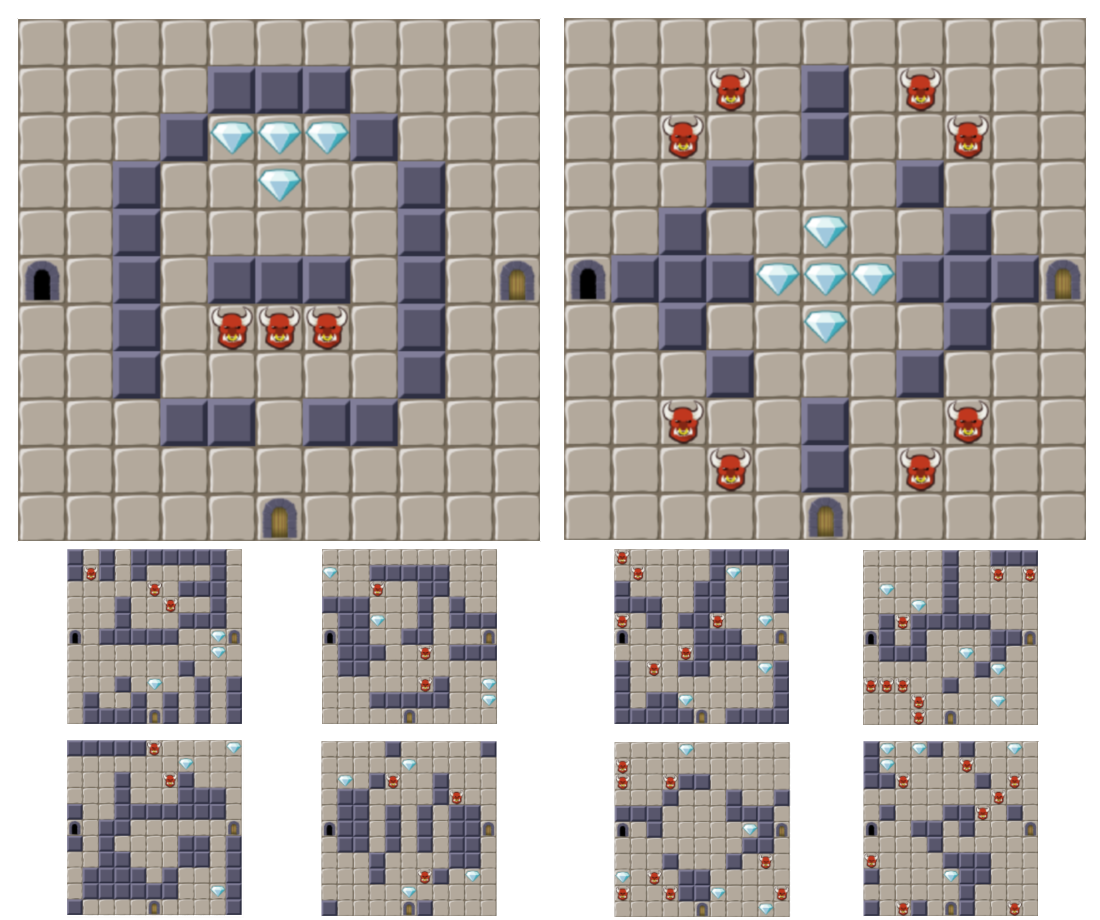
\includegraphics[scale=0.39]{Figures/figure-not-preserving}
% \caption{Sample maps from the previous version of EDD, not preserving the aesthetic changes in suggestions}
% \label{p2fig:no-aesthetic}
% \end{figure}

%The criteria can vary depending on the technique used, the goal to be reached and the evaluation to be performed. In offline generation, the algorithm tries to satisfy functional criteria (e.g. the level can be finished or all the passable tiles are accessible) \citepsecond{p2Shaker2016TheApproach,Togelius2007TowardsGames}. 
\begin{figure} [!h]
\centering
\includegraphics[width=\textwidth]{included-papers-tex/paper-2/pap2-figures/map-figure.png}
\caption{Current version of EDD and its different components. (a) Basic room, (b) different placeable tiles, (c) micro-patterns and (d) meso-patterns.}
\label{p2fig:eddy-map}
\end{figure}

As discussed by~\citepsecond{p2Baldwin2017TowardsGeneration}, it is important for a mixed-initiative SBPCG approach to evaluate the degree to which generated designs are aesthetically pleasing and interesting to the human designer. This is stressed by the designer's will to imprint and preserve their custom designs on the generated content offered by the PCG system. It is a non-trivial task to know which parts the designer wants to preserve, as well as correctly balancing human and procedurally designed content in the generated solutions. This motivates the work presented here, in which we address the need for assessing aesthetic criteria by improving both: the solution encoding mechanism and the fitness evaluation function in EDD's evolutionary algorithm.

%The overall goal of the research is to assess one of the problems that arose from the previous research's case study \citepsecond{p2Baldwin2017TowardsGeneration}, where the generator did not capture and preserve the manually edited changes done by the designers nor their aesthetic criteria in the generated suggestions. as shown in figure \ref{p2fig:no-aesthetic}. 

This paper is organized as follows: Section \ref{p2background} presents previous and related works in mixed-initiative design. Section \ref{p2approach} describes in detail the contributions of this paper and presents the results from the laboratory experiments used for validating them. Finally, Section \ref{p2conclusion} summarizes and discusses these results, as well as sets future questions to be addressed by further research in the area of aesthetic criteria and EDD.

\subsection{Related Work} \label{p2background}

\begin{figure}
\centering
\includegraphics[width=0.7\textwidth]{included-papers-tex/paper-2/pap2-figures/figure-possible-zones.png}
\caption{Different uses and possibilities that the designers can have for locking the tiles in the Room, in order to, preserve their manual changes and diverse objectives}
\label{p2fig:possible-zones}
\end{figure}


Aesthetic criteria was specified by previous research as a key feature while evaluating content, as it leads to the generation of more customized content in the eyes of the human designer, whose aesthetic vision on the content is preserved~\citepsecond{p2Liapis2012AdaptingCreation,p2Hastings2009GalacticGame,p2Machwe2006IntegratingInvestigation}.

%\emph{Tanagra}~\citepsecond{p2Tanagra2011} is used to develop 2D platform levels. The user can place different tiles, and is able to select content, which they want to keep, while Tanagra generates content around them. 

%Aesthetic criteria has been appointed by previous research as a key feature while evaluating content, as it leads to the generation of more customized content to the eyes of the human designer, whose aesthetic vision on the content is preserved \citepsecond{p2Liapis2012AdaptingCreation,Hastings2009GalacticGame,Machwe2006IntegratingInvestigation}.

Interactive evolutionary approaches incorporate human evaluation by allowing the user to select, either implicitly or explicitly, the parents of the next generation of procedurally generated individuals. In~\citepsecond{p2Zhang2015DrawCompileEvolve:Creations} system allows users to draw simple primitive shapes to seed an evolutionary algorithm and train a neural network with their aesthetic vision. In Galactic Arms Race~\citepsecond{p2Hastings2009GalacticGame} players preferences on the evolved weapons is implicitly deducted from the amount time they actively select those weapons during the gameplay.

\citepsecond{p2Liapis2012AdaptingCreation}, incorporated visual aesthetics as an evaluation of their generated spaceships by calculating different aesthetic concepts: symmetry along axes, weight distribution or design simplicity. Moreover, ~\citepsecond{p2Mario2016ACM} generated levels for Mario using symmetry as objective function, which based on their user study, were as visually pleasing as the ones created by human designers and even more than other similar approaches. 

%\citepsecond{p2Liapis2012AdaptingCreation}, incorporated visual aesthetics as an evaluation of their generated spaceships by calculating different aesthetic concepts: symmetry along axes, weight distribution or design simplicity. These were computed to produce the aesthetic fitness of a spaceship, letting the user select their preferred spaceship to adjust the weight of the different aesthetic features in the fitness calculation.


%\begin{itemize}
%  \item EDDY previous versions
%  \item Previous approaches to evaluate aesthetic criteria of the designer
%  \begin{itemize}
%  	\item Aesthetic criteria was seen as visually pleasing for the designer but that does not mean that it is the idea that the user had. For mixed-initiative the way to evaluate aesthetic criteria usually was by allowing the user to select the options that he liked the most  Show examples of Mario level generator and such.
%    \item To preserve Aesthetic criteria other authors have allow the user to initiate the evolutionary algorithm with an example (initial seed) and from there, allow the evolutionary algorithm to produce suggestions based on this.
%  \end{itemize}
%\end{itemize}

%The work presented in this paper is an extension to the ongoing research of EDD \citepsecond{p2Baldwin2017TowardsGeneration} and addresses the issue of preserving manual changes to the level and the impact of visual aesthetic criteria when designing dungeons.

\subsubsection{The Evolutionary Dungeon Designer}

EDD is a mixed-initiative authoring tool for generating dungeon rooms using a feasible-infeasible two population (fi-2pop) evolutionary approach, which is interactively evaluated and edited by a designer. The current version of EDD consists of six different building blocks that represent floors, walls, enemies, treasures, doors and entrances. This can be used by the user to brush paint and compose a NxM size room which, at its minimum, must hold one of each tile. Both the tiles and the finished room can be seen in Figure~\ref{p2fig:eddy-map}a) and b).

EDD takes the work presented in The Evolutionary World Designer~\citepsecond{p2Font2016ConstrainedAlgorithms} one step further, by procedurally generating rooms and their specific content. EDD's EA follows the approach of~\citepsecond{p2Liapis2012AdaptingCreation} using the evaluation of the user to change the internal evaluation and configuration of the system. Its fitness evaluation is driven by the use of game design micro- and meso- patterns, as shown in Figure \ref{p2fig:eddy-map} c) and d). A detailed description of EDD's pattern-based fitness, genetic algorithm and mixed-initiative approach can be found in \citepsecond{p2Baldwin2017Mixed-initiativePatterns} and \citepsecond{p2Baldwin2017TowardsGeneration}.

\subsection{Assessing Aesthetic Criteria} \label{p2approach}

\begin{figure}
\centering
\includegraphics[width=0.7\textwidth]{included-papers-tex/paper-2/pap2-figures/map-representation-figure-test.png}
\caption{A sample edited room (a) with its division into zones (b) based on the tiles locked by the user. Suggestions preserve these locked tiles (c). The room and its zones are internally represented with a tree structure (d), where the leaf nodes (green) are the valid candidates to operate within an individual.}
\label{p2fig:map-representation}
\end{figure}

Our approach is divided in two; on one side, the algorithm implicitly has control over different aesthetic criteria using the edited room as a base to measure symmetry and similarity for the EA. On the other side, the designer was given control over what they wanted to preserve by being able to select tiles in the room to be immutable (i.e. not changeable in following generations).

\subsubsection{Preserving Custom Aesthetic Structures}

%To preserve the aesthetic criteria of a designer's edited room, we give him/her the ability to manually lock custom structures in it, preserving these in the upcoming the next suggestions. This is possible by incorporating a new brush which is used as a complementary modifier when editing the room. The designer can now lock any range of tiles, making it possible to preserve individual tiles, shapes, patterns, routes and even design patterns as shown in Figure \ref{p2fig:possible-zones}. 
To preserve the aesthetic criteria of a designer's edited room, we give the users the ability to manually lock custom structures in it, preserving these in the upcoming suggestions. This is possible by incorporating a new brush which is used as a complementary modifier when editing the room. The designer can now lock any range of tiles, making it possible to preserve individual tiles, shapes, patterns, routes and even design patterns as shown in Figure~\ref{p2fig:possible-zones}.

The process to subdivide the room is straightforward; the designer is presented with the room to be edited, and by using the lock brush, the room seamlessly subdivides and creates zones, which classifies the room's tiles into two sets: the immutable tiles (i.e. invalid or locked) and the mutable tiles (i.e. valid or unlocked).

An individual's genotype is now changed from a direct encoding (each tile is a gene) to a semi-direct encoding using a tree structure, with the nodes of the tree as different zones of the room, constructed from the mutable and immutable tiles, and the leaf nodes, only containing sets of mutable tiles, as candidates to be used for crossing and mutation. Figure~\ref{p2fig:map-representation} shows the room, it's division into zones and the tree representation used by the EA. 

The advantages of this representation are that it allows the EA to reduce the search space by only considering valid zones of the room, and improves the crossover operator by allowing the exchange of irregular shapes between individuals along different parts of the room.

%An individual's genotype is now changed from a direct encoding (each tile is a gene) to a semi-direct encoding using a tree structure, with the nodes of the tree as different sections of the room and the leaf nodes as candidates to be used for crossing and mutation. Figure~\ref{p2fig:map-representation} shows the room, it's division into zones and the tree representation used by the EA. This change in the individual representation improves the crossover operator by allowing the exchange of irregular shapes between individuals along different parts of the room. This results in an increased presence of custom (user-shaped) building blocks among the generated offspring.

In practice, this solution allows users to preserve any aesthetic change (either significant or detailed) that they want to keep in further generations, while still receiving novel suggestions created following the pattern-based fitness function. It also means that the construction of the dungeon can be performed differently: instead of manually editing a room first to later generate appealing solutions based on it, the user can now start from a suggestion, selecting parts of it that look promising that are kept through subsequent generations, until the user's needs and criteria are met.

%In practice, this solution allows users to preserve any aesthetic change (either significant or detailed) that they want to keep in further generations, while still receiving novel suggestions created following the pattern-based fitness function. It also means that the construction of the dungeon can be performed differently: instead of manually editing a room first to later generate appealing solutions based on it, the user can now start from a suggestion, selecting parts of it that look promising that are kept through the following generations of procedurally generated suggestions, until the user's needs and criteria are met.

%In practice, this solution allows users to preserve any aesthetic change (either significant or detailed) that they want to keep in further generations, while still receiving novel suggestions created following the pattern-based fitness function. It also means that the construction of the dungeon can be performed differently: instead of manually editing a room first to later generate appealing solutions based on it, the user can now start from a suggestion, selecting parts of it that look promising that are kept through the following generations of procedurally generated suggestions, until one meets his/her needs and criteria.

\subsubsection{Evaluating Symmetry and Similarity}

\begin{figure}
\centering
\includegraphics[width=0.7\textwidth]{included-papers-tex/paper-2/pap2-figures/DifferentSymmetry.png}
\caption{Different types of symmetry evaluated}
\label{p2fig:symmetry-types}
\end{figure}

While the pattern-based fitness function worked well for functionality purposes, it did not consider nor capture any aesthetic aspects into it. Therefore, in order to consider and preserve visual aesthetic criteria, we evaluate the rooms for their symmetry  along the X and Y axes, backslash and front slash diagonal as shown in Figure \ref{p2fig:symmetry-types} and calculate the similarity that subsequent individuals had in comparison with the original edited room. For simplicity, we differentiate the room by impassable (i.e. walls) and passable (i.e. floor, treasure and enemy) tiles.

%In order to implicitly consider and preserve visual aesthetics criteria, we evaluate the rooms for their symmetry  along the X and Y axes, backslash and front slash diagonal as shown in Figure \ref{p2fig:symmetry-types} and calculate the similarity that subsequent individuals had in comparison with the original edited room. For simplicity, we differentiate the room by impassable (i.e. walls) and passable (i.e. floor, treasure and enemy) tiles.

%In order to implicitly consider and preserve visual aesthetics criteria, we evaluated the rooms for their symmetry  along the X and Y axes, backslash and front slash diagonal as shown in Figure \ref{p2fig:symmetry-types} and calculated the similarity that subsequent individuals had regarding the original edited room. For simplicity, we differentiated the room by unpassable (i.e. walls) and passable (i.e. floor, treasure and enemy) tiles.

\paragraph{Symmetry evaluation}

%unpassable
%To calculate the symmetry of a room we evaluate the impassable tiles of one side against their corresponding tile on the other side for the X and Y axes and diagonals. The highest symmetric value is then used to calculate a curve ranging from 0 to 1, using equation \ref{p2eq:Symmetry}.

To calculate the symmetry of a room we evaluate the impassable tiles of one side against their corresponding tile on the other side for the X and Y axes and diagonals. The highest symmetric value is then used in equation~\ref{p2eq:Symmetry} to calculate the fitness.

\begin{equation} \label{p2eq:Symmetry}
f_{symmetry} = \frac{highestSymmetricValue} {totalWalls}
\end{equation}

Equation~\ref{p2eq:Symmetry} allow us to calculate symmetry while also preventing the favoring of more walls. Once calculated, we weight the result into the individual's fitness, and as consequence it would favor more or less symmetric rooms and preserve the room's configuration as it can be seen in Figure~\ref{p2fig:symmetry-result}.

\begin{figure}
\centering
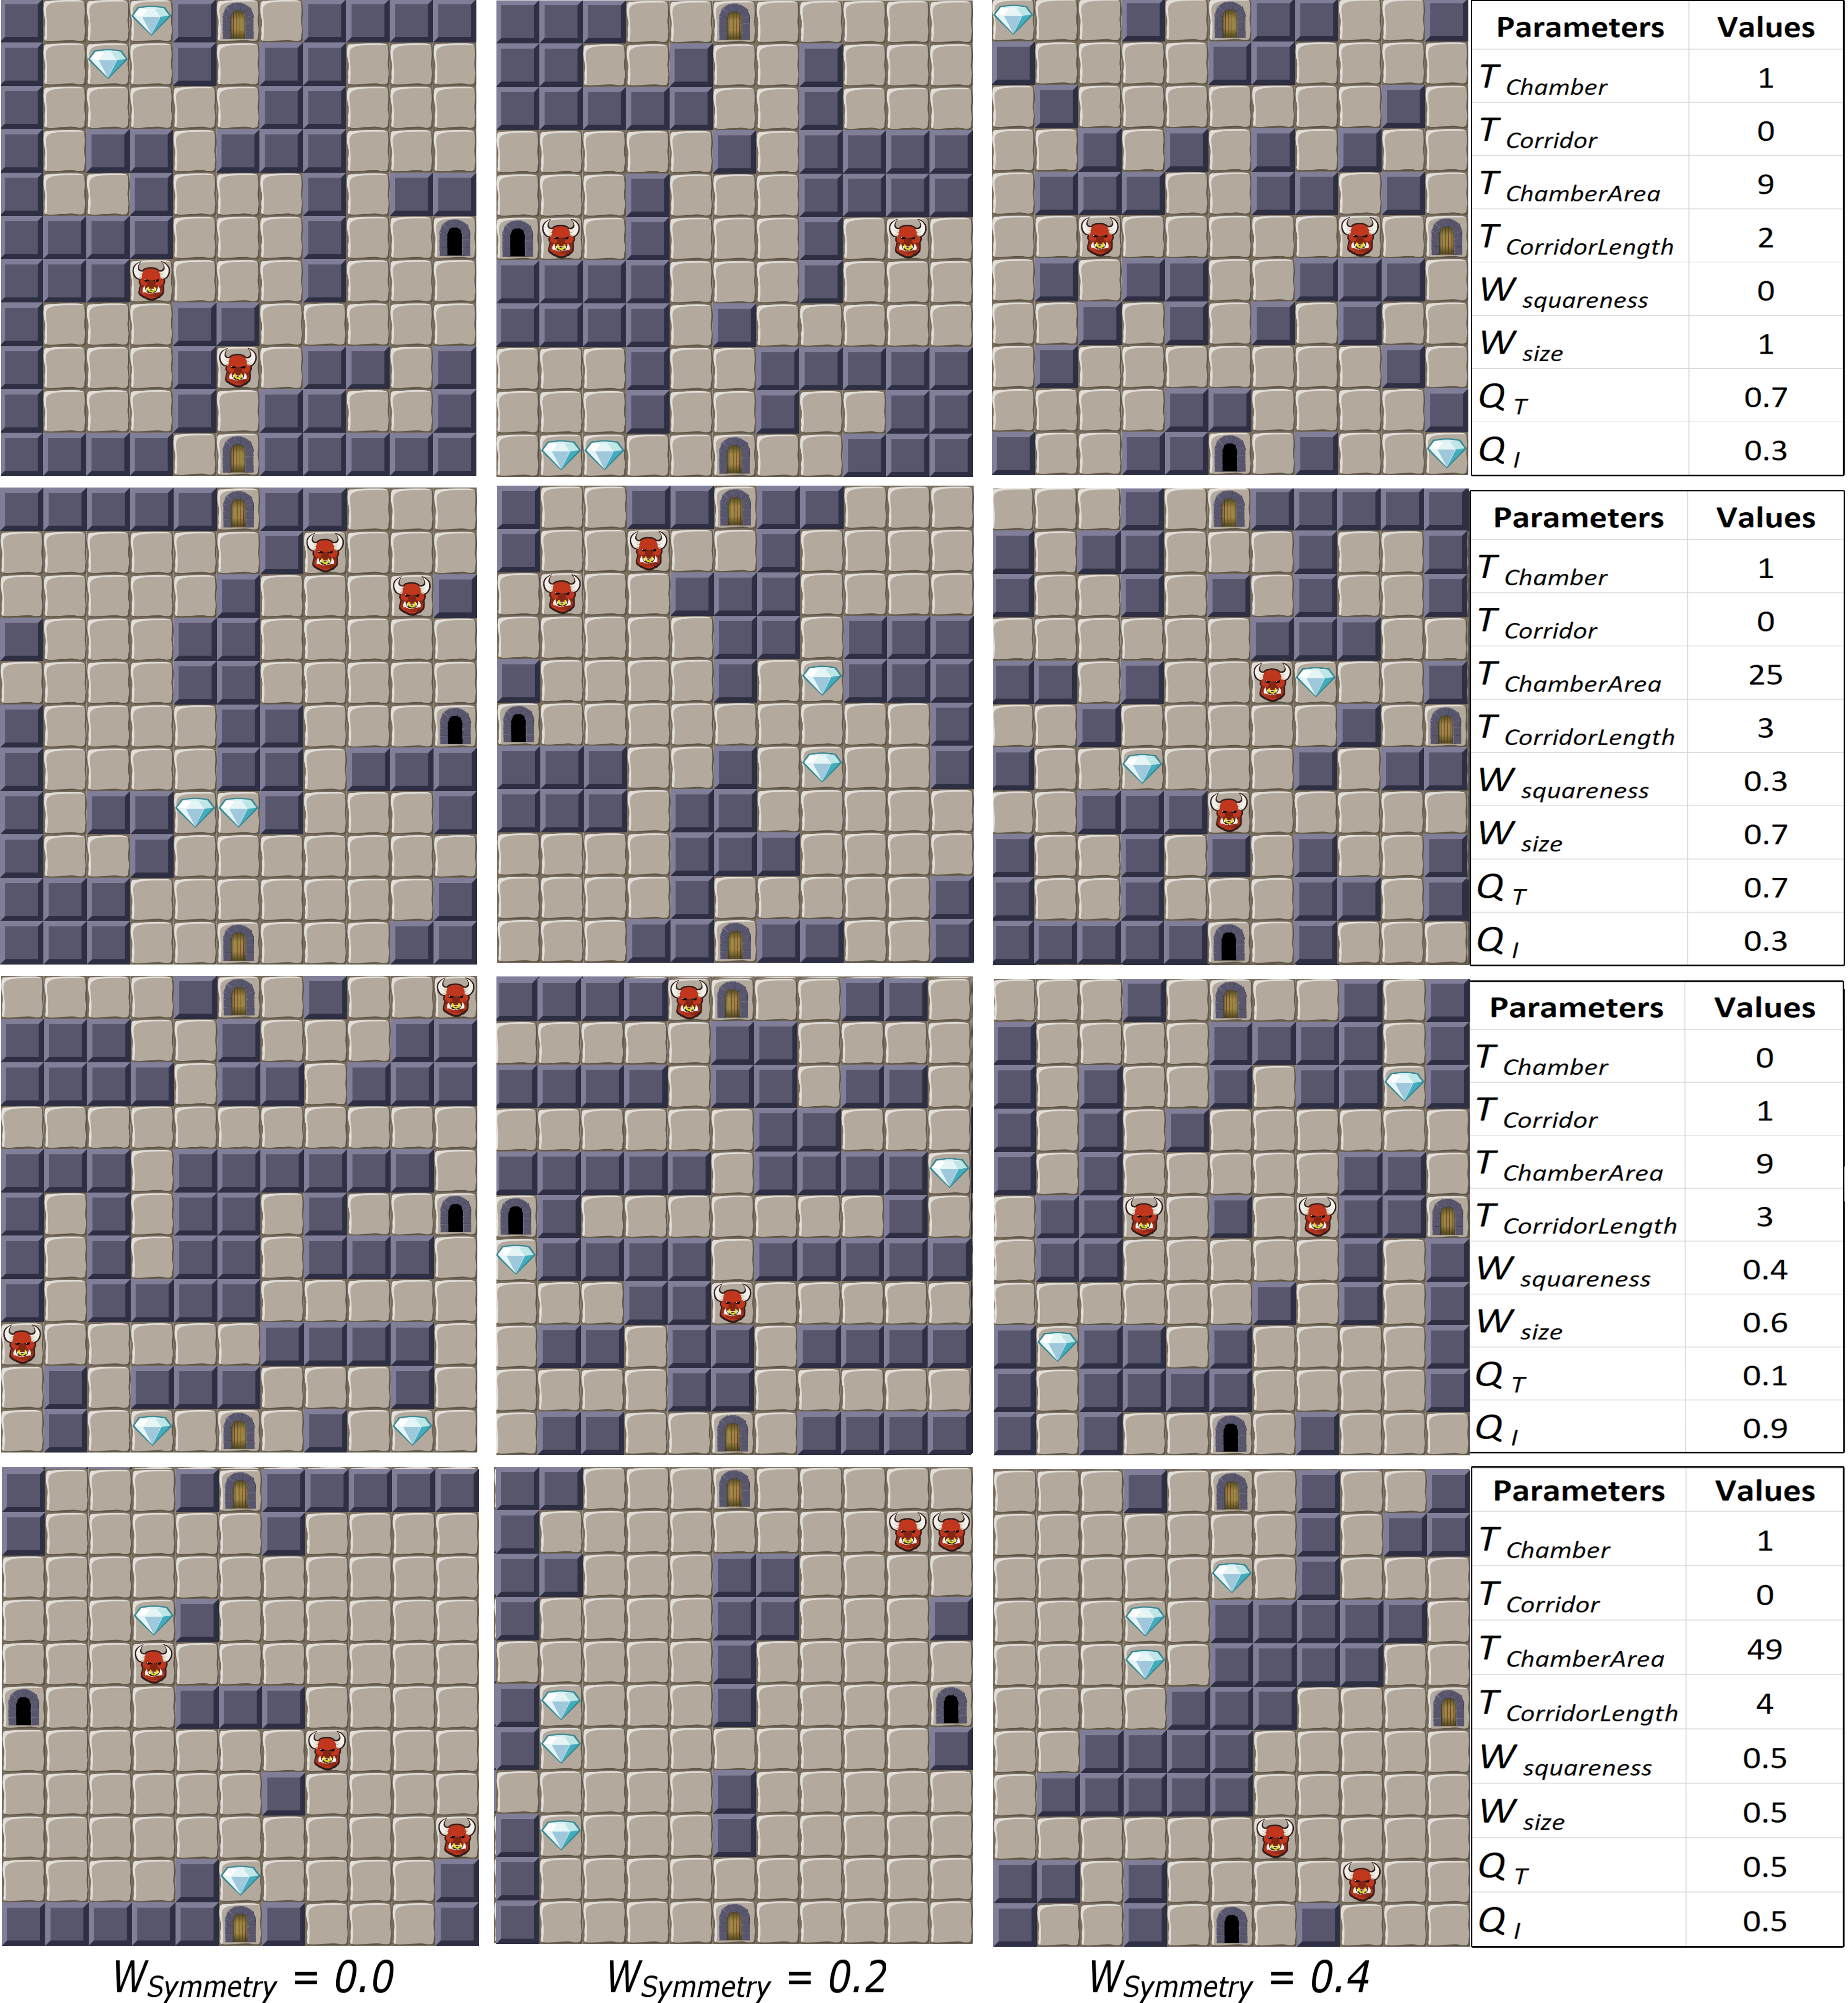
\includegraphics[width=0.7\textwidth]{included-papers-tex/paper-2/pap2-figures/symmetry-result-figuer.png}
\caption{Each row shows three results (\(W_{symmetry}=0, W_{symmetry}=0.2, W_{symmetry}=0.4\) ) produced under the settings displayed on the rightmost column. Metrics adapted from~\protect\citepsecond{p2Baldwin2017Mixed-initiativePatterns}.}
\label{p2fig:symmetry-result}
\end{figure}

\paragraph{Similarity evaluation}

The similarity value between an edited room and successive evolved rooms is calculated by comparing every tile in the original with the corresponding tile in subsequent individuals. Once the total amount of equal tiles is known, we calculate the similarity percentage based on the total amount of tiles, following equation~\ref{p2eq:ProcentSimilar}. 

\begin{equation} \label{p2eq:ProcentSimilar}
similarityPercentage = \frac{totalTiles - notSimilarTiles} {totalTiles}
\end{equation}

%In order for the similarity percentage to be useful we introduced \(idealSimilarityPercentage\) as a parameter related to how similar we want the individuals to be, and use it to normalize the final \(f_{similarity}\) as shown in equation~\ref{p2eq:FSimilarity} or if \(SimilarityPercentage\) was higher then we use~\ref{p2eq:FSimilarity2}.

%\begin{equation} \label{p2eq:FSimilarity}
%f_{similarity} = \frac{SimilarityPercentage} {idealSimilarityPercentage}
%\end{equation}

%\begin{equation} \label{p2eq:FSimilarity2}
%f_{similarity} = \frac{1 - SimilarityPercentage} {1 - idealSimilarityPercentage}
%\end{equation}

We introduced a second parameter called \(idealSimilarity\), which represents how similar we want the individuals to be. Following equation~\ref{p2eq:FSimilarity} we measured the error between both similarities and used it as the similarity fitness. 

\begin{equation} \label{p2eq:FSimilarity}
f_{similarity} = 1 - \left |idealSimilarity - SimilarityPercentage \right |
\end{equation}

The result of incorporating the similarity evaluation into the final fitness is shown in Figure~\ref{p2fig:similarity-result} where is observable that depending on the \(idealSimilarityPercentage\) the original room goes from having a slight variation to start losing its resemblance.

\begin{figure}
\centering
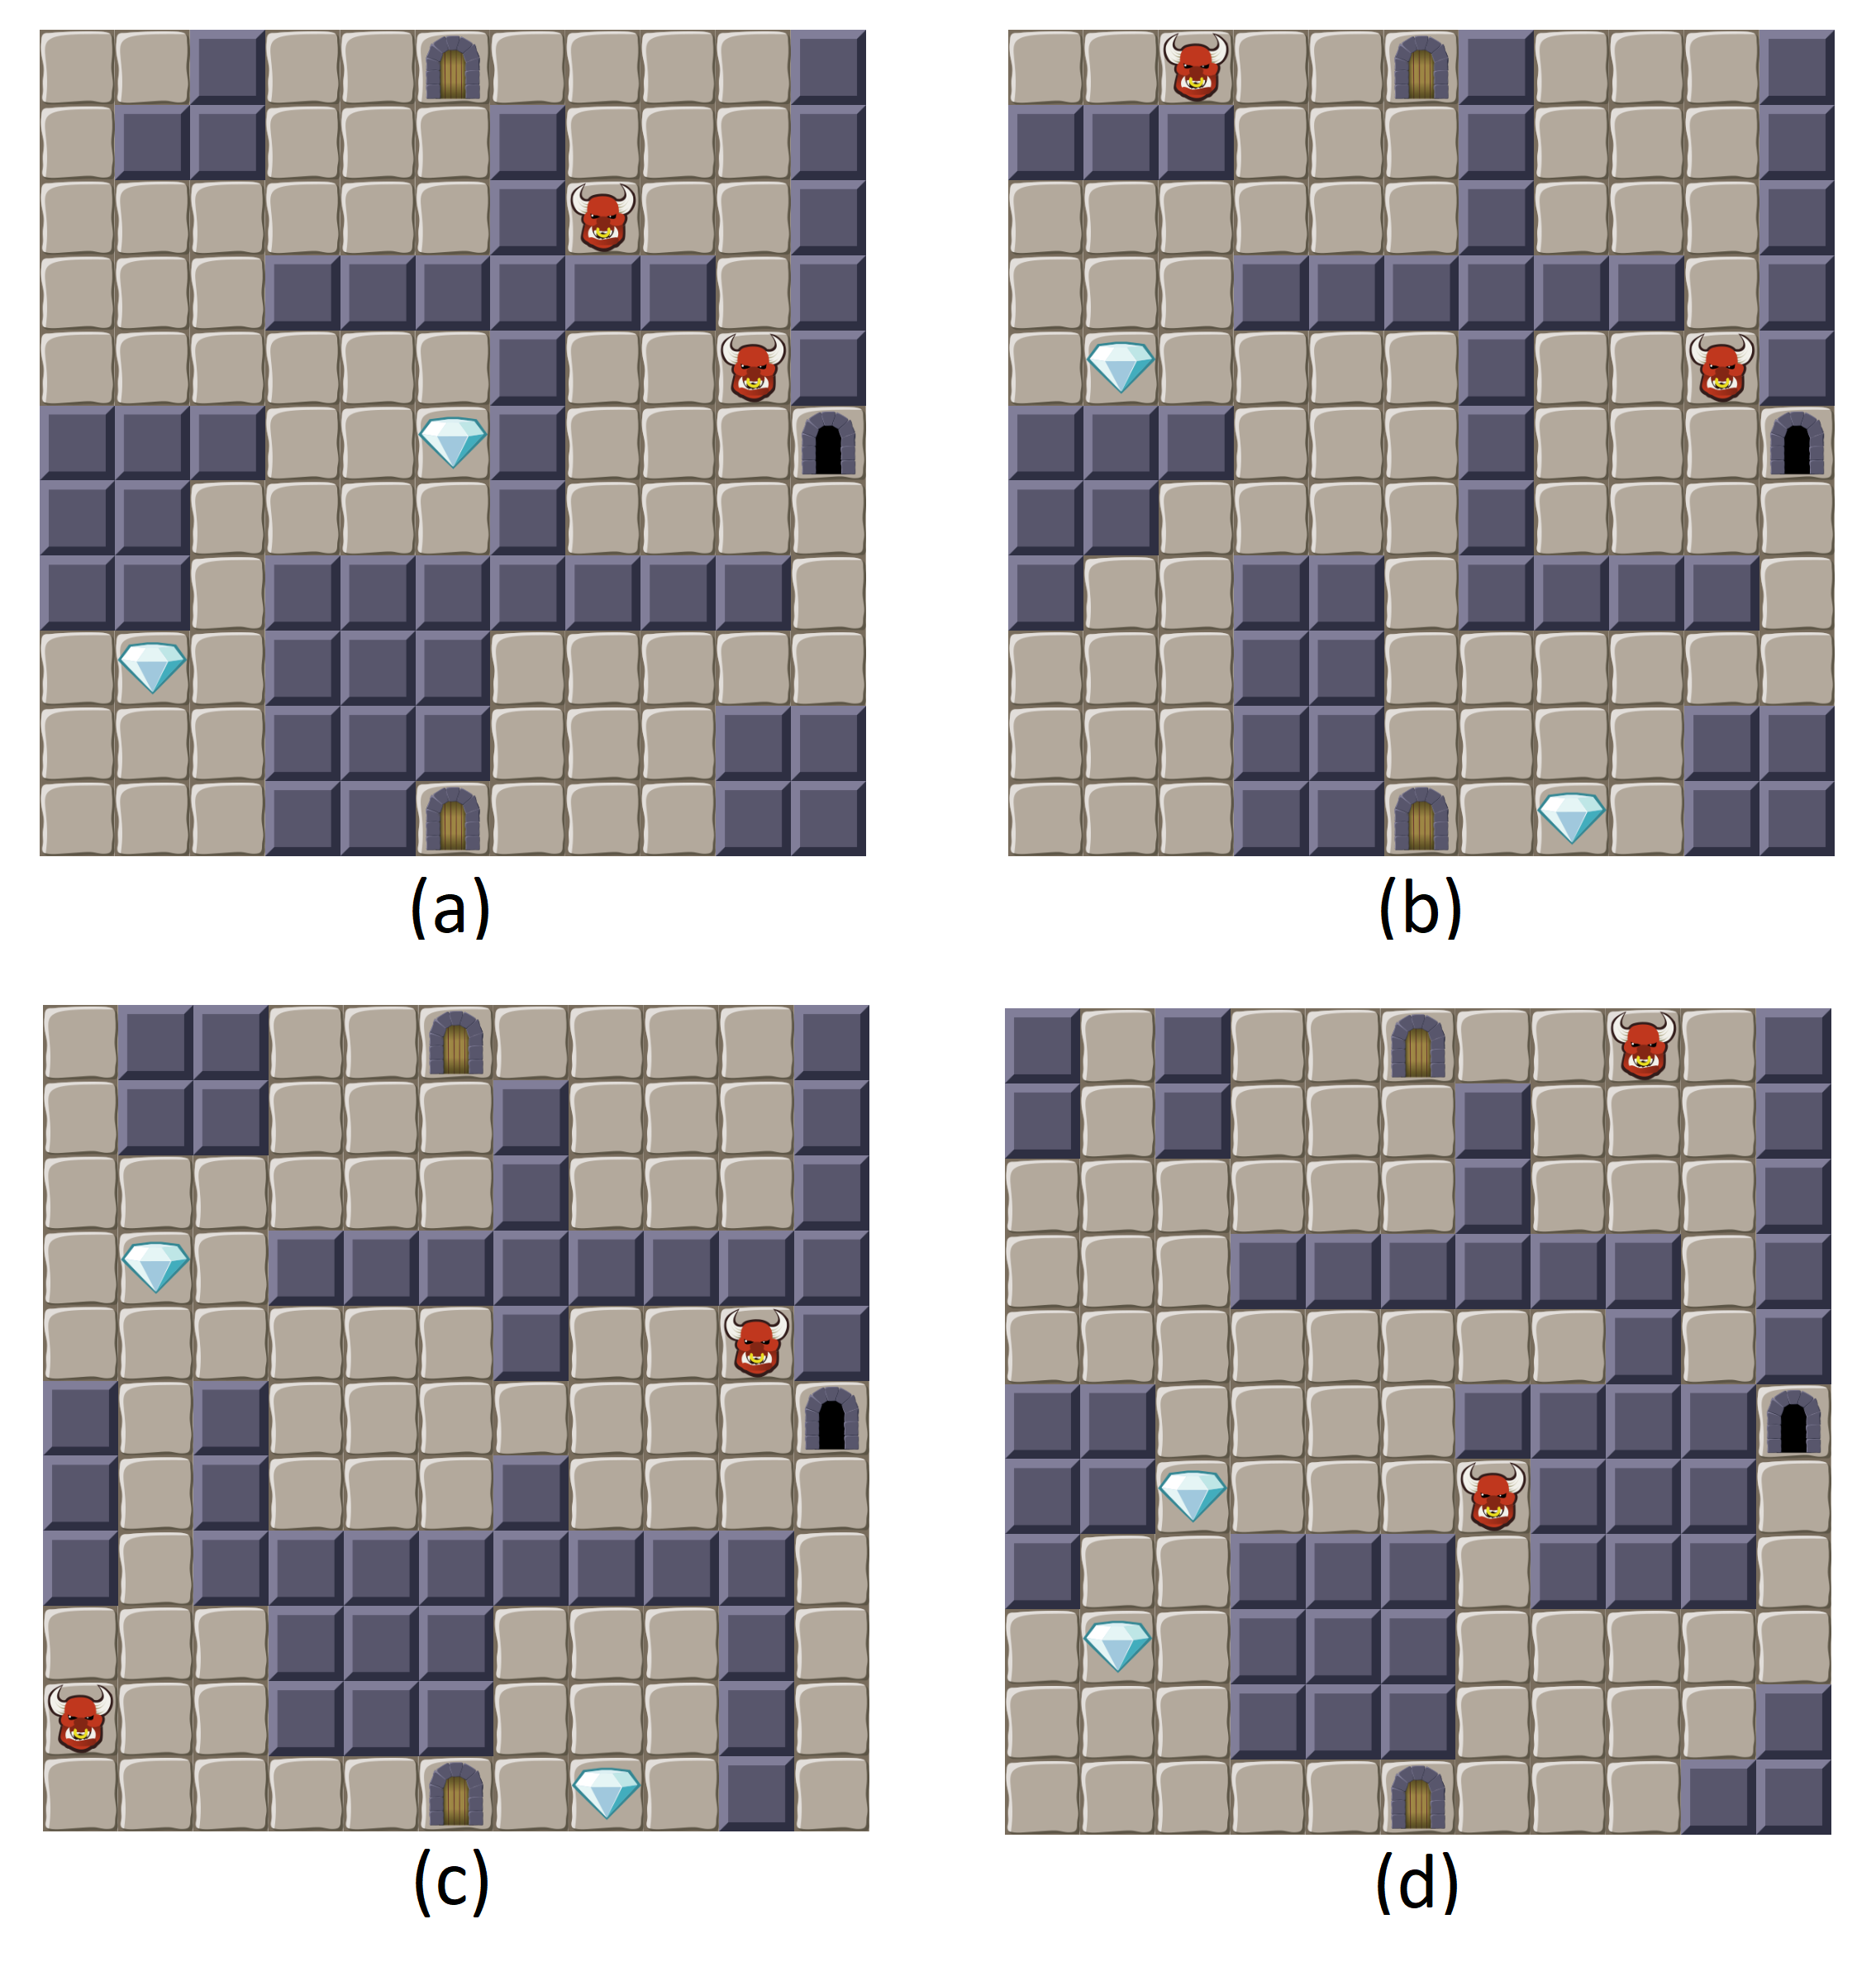
\includegraphics[width=0.7\textwidth]{included-papers-tex/paper-2/pap2-figures/figure-similarity.png}
\caption{(a) Sample original room and the evolved solutions with different \(idealSimilarity\) values in order: (b)~0.95, (c) 0.90 and (d) 0.85.}
\label{p2fig:similarity-result}
\end{figure}

Finally and expanding over the previous work on EDD~\citepsecond{p2Baldwin2017TowardsGeneration}, these calculations (i.e. \(f_{symmetry}\) and \(f_{similarity}\)) are included into the existing fitness evaluation of an individual as shown in equation \ref{p2eq:SiSyFitness}. \(f_{inventorial}\) and \(f_{spacial}\), evaluates the overall layout of the room, and the frequency and quality of the design patterns in the room, respectively. An in-depth explanation of both can be found in~\citepsecond{p2Baldwin2017TowardsGeneration}.

%Finally and expanding over the previous work on EDD~\citepsecond{p2Baldwin2017TowardsGeneration}, these calculations are included into the existing fitness evaluation of an individual as shown in equation \ref{p2eq:SiSyFitness}.

\begin{equation} \label{p2eq:SiSyFitness}
\begin{split}
f_{fitness}(r) & = (\frac{a}{10}f_{inventorial}(r) \,+ \, \frac{b}{10}f_{spacial}(r) \\ 
 & \, + \; \frac{c}{10}f_{symmetry}(r)) \ * \ f_{similarity}(r)
\end{split}
\end{equation}

\subsection{Conclusions and Future Work} \label{p2conclusion}

In this paper, we have presented the advancements done on EDD in relation to the evolutionary system with different evaluations, encoding, genotype representation and strategies that aims on preserving and consider the designer's aesthetic criteria.

By introducing the capability of locking sections of a room, we changed the individual's encoding from direct to semi-direct, and in turn, offered new and easier possibilities to perform different operations to the individuals, as well as, allowing the designer to preserve individual tiles, shapes, routes and even design patterns.

%By changing the encoding of the evolutionary algorithm from direct to semi-direct encoding we opened the possibilities to perform different operations to the individuals, as well as a fair way of preserving the sections of the map which were considered important, significant and unchangeable by the designer. As result, the generator has increased on controllability at expenses of expressiveness. Moreover, this approach allows the designer not only to lock and preserve interesting aesthetical changes done in the map but also indirectly, is able to preserve routes and design patterns.

Moreover, we successfully integrated and produced rooms evaluated  on symmetry and similarity that held the overlying structure of the micro-patterns. The added evaluations establishes the path to preserve and consider more in-depth the designers criteria and produce personalized work that accurately transmit the ideas and intentions of the designer.

%In the end, we successfully integrated and produced dungeon levels which, held the overlying structure of the micro-patterns and symmetry together \textbf{(here is missing the part of the similarity)}. Moreover, the added evaluations to the fitness of each individual allows us to establish the path to preserve and consider more in-depth the designers criteria and produce a more personalized work that accurately transmit the ideas and intentions of the designer.

We aim to more throughly evaluate the system by incorporate the three techniques into a user study, similar to the one done by~\citepsecond{p2Baldwin2017TowardsGeneration} to validate the tool's capacity on assessing the designer's criteria. It would be interesting to add more aesthetic concepts to evaluate the produced content, for instance, density, simplicity, sparseness and individuality.

%We aim to further evaluate the system with different configurations and observe how the different fitness functions can interact and cooperate with each other to create more interesting content, as well as, joining both approaches for a case study, similar to the one done by Baldwin et al \citepsecond{p2Baldwin2017TowardsGeneration}. It would be interesting to continue using aesthetic concepts, for instance, density, simplicity, sparseness and individuality, to evaluate the content 

The subdivision of the map could be extended to perform a parallel evolution on the custom aesthetic structures locked by the designers and propose interesting variations. Moreover, a zone analysis could be introduced to increase the dungeon's knowledge for the designer by suggesting changes to fulfill different player models, similar to Holmg\r{a}rd's approach~\citepsecond{p2Holmgard2014EvolvingModeling}, or paths and statistics. Finally, we would like to explore different types of representations towards more generative encodings to test, compare and measure the differences and advantages of the resulting maps.

%Further use the division of the map by performing zone analysis, which could result on suggesting changes to the designers in order to fulfill different player models, similar to Holmg\r{a}rd's approach \citepsecond{p2Holmgard2014EvolvingModeling} or do a separated evolution on the manually locked tiles providing the designers with interesting shapes and patterns. Finally, we would like to go down the road towards more indirect encodings and test different approaches and, compare and measure the differences and advantages of the resulting maps.

%\subsection{Future Work} \label{p2future-work}

We aim to further evaluate the system with different configurations and observe how the different fitness functions can interact and cooperate with each other to create more interesting content, as well as, joining both approaches for a case study, similar to the one done by Baldwin et al \citepsecond{p2Baldwin2017TowardsGeneration}. It would be interesting to continue using aesthetic concepts, for instance, density, simplicity, sparseness and individuality, to evaluate the content 

Further use the division of the map by performing zone analysis, which could result on suggesting changes to the designers in order to fulfill different player models, similar to Holmg\r{a}rd's approach \citepsecond{p2Holmgard2014EvolvingModeling} or do a separated evolution on the manually locked tiles providing the designers with interesting shapes and patterns. Finally, we would like to go down the road towards more indirect encodings and test different approaches and, compare and measure the differences and advantages of the resulting maps.
% \section{Related Work} \label{p2background}

\begin{figure}
\includegraphics[scale=0.16]{Figures/figure-possible-zones}
\caption{Different uses and possibilities that the designers can have for locking the tiles in the Room, in order to, preserve their manual changes and diverse objectives}
\label{p2fig:possible-zones}
\end{figure}


Aesthetic criteria was specified by previous research as a key feature while evaluating content, as it leads to the generation of more customized content in the eyes of the human designer, whose aesthetic vision on the content is preserved~\cite{Liapis2012AdaptingCreation,Hastings2009GalacticGame,Machwe2006IntegratingInvestigation}.

%\emph{Tanagra}~\cite{Tanagra2011} is used to develop 2D platform levels. The user can place different tiles, and is able to select content, which they want to keep, while Tanagra generates content around them. 

%Aesthetic criteria has been appointed by previous research as a key feature while evaluating content, as it leads to the generation of more customized content to the eyes of the human designer, whose aesthetic vision on the content is preserved \cite{Liapis2012AdaptingCreation,Hastings2009GalacticGame,Machwe2006IntegratingInvestigation}.

Interactive evolutionary approaches incorporate human evaluation by allowing the user to select, either implicitly or explicitly, the parents of the next generation of procedurally generated individuals. In~\citet{Zhang2015DrawCompileEvolve:Creations} system allows users to draw simple primitive shapes to seed an evolutionary algorithm and train a neural network with their aesthetic vision. In Galactic Arms Race~\cite{Hastings2009GalacticGame} players preferences on the evolved weapons is implicitly deducted from the amount time they actively select those weapons during the gameplay.

\citet{Liapis2012AdaptingCreation}, incorporated visual aesthetics as an evaluation of their generated spaceships by calculating different aesthetic concepts: symmetry along axes, weight distribution or design simplicity. Moreover, ~\citet{Mario2016ACM} generated levels for Mario using symmetry as objective function, which based on their user study, were as visually pleasing as the ones created by human designers and even more than other similar approaches. 

%\citet{Liapis2012AdaptingCreation}, incorporated visual aesthetics as an evaluation of their generated spaceships by calculating different aesthetic concepts: symmetry along axes, weight distribution or design simplicity. These were computed to produce the aesthetic fitness of a spaceship, letting the user select their preferred spaceship to adjust the weight of the different aesthetic features in the fitness calculation.


%\begin{itemize}
%  \item EDDY previous versions
%  \item Previous approaches to evaluate aesthetic criteria of the designer
%  \begin{itemize}
%  	\item Aesthetic criteria was seen as visually pleasing for the designer but that does not mean that it is the idea that the user had. For mixed-initiative the way to evaluate aesthetic criteria usually was by allowing the user to select the options that he liked the most  Show examples of Mario level generator and such.
%    \item To preserve Aesthetic criteria other authors have allow the user to initiate the evolutionary algorithm with an example (initial seed) and from there, allow the evolutionary algorithm to produce suggestions based on this.
%  \end{itemize}
%\end{itemize}

%The work presented in this paper is an extension to the ongoing research of EDD \cite{Baldwin2017TowardsGeneration} and addresses the issue of preserving manual changes to the level and the impact of visual aesthetic criteria when designing dungeons.

\subsection{The Evolutionary Dungeon Designer}

EDD is a mixed-initiative authoring tool for generating dungeon rooms using a feasible-infeasible two population (fi-2pop) evolutionary approach, which is interactively evaluated and edited by a designer. The current version of EDD consists of six different building blocks that represent floors, walls, enemies, treasures, doors and entrances. This can be used by the user to brush paint and compose a NxM size room which, at its minimum, must hold one of each tile. Both the tiles and the finished room can be seen in Figure~\ref{p2fig:eddy-map}a) and b).

EDD takes the work presented in The Evolutionary World Designer~\cite{Font2016ConstrainedAlgorithms} one step further, by procedurally generating rooms and their specific content. EDD's EA follows the approach of~\citet{Liapis2012AdaptingCreation} using the evaluation of the user to change the internal evaluation and configuration of the system. Its fitness evaluation is driven by the use of game design micro- and meso- patterns, as shown in Figure \ref{p2fig:eddy-map} c) and d). A detailed description of EDD's pattern-based fitness, genetic algorithm and mixed-initiative approach can be found in \cite{Baldwin2017Mixed-initiativePatterns} and \cite{Baldwin2017TowardsGeneration}.
% \section{Assessing Aesthetic Criteria} \label{p2approach}

\begin{figure}
\includegraphics[scale=0.2]{Figures/map-representation-figure-test}
\caption{A sample edited room (a) with its division into zones (b) based on the tiles locked by the user. Suggestions preserve these locked tiles (c). The room and its zones are internally represented with a tree structure (d), where the leaf nodes (green) are the valid candidates to operate within an individual.}
\label{p2fig:map-representation}
\end{figure}

Our approach is divided in two; on one side, the algorithm implicitly has control over different aesthetic criteria using the edited room as a base to measure symmetry and similarity for the EA. On the other side, the designer was given control over what they wanted to preserve by being able to select tiles in the room to be immutable (i.e. not changeable in following generations).

\subsection{Preserving Custom Aesthetic Structures}

%To preserve the aesthetic criteria of a designer's edited room, we give him/her the ability to manually lock custom structures in it, preserving these in the upcoming the next suggestions. This is possible by incorporating a new brush which is used as a complementary modifier when editing the room. The designer can now lock any range of tiles, making it possible to preserve individual tiles, shapes, patterns, routes and even design patterns as shown in Figure \ref{p2fig:possible-zones}. 
To preserve the aesthetic criteria of a designer's edited room, we give the users the ability to manually lock custom structures in it, preserving these in the upcoming suggestions. This is possible by incorporating a new brush which is used as a complementary modifier when editing the room. The designer can now lock any range of tiles, making it possible to preserve individual tiles, shapes, patterns, routes and even design patterns as shown in Figure~\ref{p2fig:possible-zones}.

The process to subdivide the room is straightforward; the designer is presented with the room to be edited, and by using the lock brush, the room seamlessly subdivides and creates zones, which classifies the room's tiles into two sets: the immutable tiles (i.e. invalid or locked) and the mutable tiles (i.e. valid or unlocked).

An individual's genotype is now changed from a direct encoding (each tile is a gene) to a semi-direct encoding using a tree structure, with the nodes of the tree as different zones of the room, constructed from the mutable and immutable tiles, and the leaf nodes, only containing sets of mutable tiles, as candidates to be used for crossing and mutation. Figure~\ref{p2fig:map-representation} shows the room, it's division into zones and the tree representation used by the EA. 

The advantages of this representation are that it allows the EA to reduce the search space by only considering valid zones of the room, and improves the crossover operator by allowing the exchange of irregular shapes between individuals along different parts of the room.

%An individual's genotype is now changed from a direct encoding (each tile is a gene) to a semi-direct encoding using a tree structure, with the nodes of the tree as different sections of the room and the leaf nodes as candidates to be used for crossing and mutation. Figure~\ref{p2fig:map-representation} shows the room, it's division into zones and the tree representation used by the EA. This change in the individual representation improves the crossover operator by allowing the exchange of irregular shapes between individuals along different parts of the room. This results in an increased presence of custom (user-shaped) building blocks among the generated offspring.

In practice, this solution allows users to preserve any aesthetic change (either significant or detailed) that they want to keep in further generations, while still receiving novel suggestions created following the pattern-based fitness function. It also means that the construction of the dungeon can be performed differently: instead of manually editing a room first to later generate appealing solutions based on it, the user can now start from a suggestion, selecting parts of it that look promising that are kept through subsequent generations, until the user's needs and criteria are met.

%In practice, this solution allows users to preserve any aesthetic change (either significant or detailed) that they want to keep in further generations, while still receiving novel suggestions created following the pattern-based fitness function. It also means that the construction of the dungeon can be performed differently: instead of manually editing a room first to later generate appealing solutions based on it, the user can now start from a suggestion, selecting parts of it that look promising that are kept through the following generations of procedurally generated suggestions, until the user's needs and criteria are met.

%In practice, this solution allows users to preserve any aesthetic change (either significant or detailed) that they want to keep in further generations, while still receiving novel suggestions created following the pattern-based fitness function. It also means that the construction of the dungeon can be performed differently: instead of manually editing a room first to later generate appealing solutions based on it, the user can now start from a suggestion, selecting parts of it that look promising that are kept through the following generations of procedurally generated suggestions, until one meets his/her needs and criteria.

\subsection{Evaluating Symmetry and Similarity}

\begin{figure}
\includegraphics[scale=0.09]{Figures/DifferentSymmetry}
\caption{Different types of symmetry evaluated}
\label{p2fig:symmetry-types}
\end{figure}

While the pattern-based fitness function worked well for functionality purposes, it did not consider nor capture any aesthetic aspects into it. Therefore, in order to consider and preserve visual aesthetic criteria, we evaluate the rooms for their symmetry  along the X and Y axes, backslash and front slash diagonal as shown in Figure \ref{p2fig:symmetry-types} and calculate the similarity that subsequent individuals had in comparison with the original edited room. For simplicity, we differentiate the room by impassable (i.e. walls) and passable (i.e. floor, treasure and enemy) tiles.

%In order to implicitly consider and preserve visual aesthetics criteria, we evaluate the rooms for their symmetry  along the X and Y axes, backslash and front slash diagonal as shown in Figure \ref{p2fig:symmetry-types} and calculate the similarity that subsequent individuals had in comparison with the original edited room. For simplicity, we differentiate the room by impassable (i.e. walls) and passable (i.e. floor, treasure and enemy) tiles.

%In order to implicitly consider and preserve visual aesthetics criteria, we evaluated the rooms for their symmetry  along the X and Y axes, backslash and front slash diagonal as shown in Figure \ref{p2fig:symmetry-types} and calculated the similarity that subsequent individuals had regarding the original edited room. For simplicity, we differentiated the room by unpassable (i.e. walls) and passable (i.e. floor, treasure and enemy) tiles.

\subsubsection{Symmetry evaluation}

%unpassable
%To calculate the symmetry of a room we evaluate the impassable tiles of one side against their corresponding tile on the other side for the X and Y axes and diagonals. The highest symmetric value is then used to calculate a curve ranging from 0 to 1, using equation \ref{p2eq:Symmetry}.

To calculate the symmetry of a room we evaluate the impassable tiles of one side against their corresponding tile on the other side for the X and Y axes and diagonals. The highest symmetric value is then used in equation~\ref{p2eq:Symmetry} to calculate the fitness.

\begin{equation} \label{p2eq:Symmetry}
f_{symmetry} = \frac{highestSymmetricValue} {totalWalls}
\end{equation}

Equation~\ref{p2eq:Symmetry} allow us to calculate symmetry while also preventing the favoring of more walls. Once calculated, we weight the result into the individual's fitness, and as consequence it would favor more or less symmetric rooms and preserve the room's configuration as it can be seen in Figure~\ref{p2fig:symmetry-result}.

\begin{figure}
\includegraphics[scale=0.082]{Figures/symmetry-result-figuer}
\caption{Each row shows three results (\(W_{symmetry}=0, W_{symmetry}=0.2, W_{symmetry}=0.4\) ) produced under the settings displayed on the rightmost column. Metrics adapted from \cite{Baldwin2017Mixed-initiativePatterns}.}
\label{p2fig:symmetry-result}
\end{figure}

\subsubsection{Similarity evaluation}

The similarity value between an edited room and successive evolved rooms is calculated by comparing every tile in the original with the corresponding tile in subsequent individuals. Once the total amount of equal tiles is known, we calculate the similarity percentage based on the total amount of tiles, following equation~\ref{p2eq:ProcentSimilar}. 

\begin{equation} \label{p2eq:ProcentSimilar}
similarityPercentage = \frac{totalTiles - notSimilarTiles} {totalTiles}
\end{equation}

%In order for the similarity percentage to be useful we introduced \(idealSimilarityPercentage\) as a parameter related to how similar we want the individuals to be, and use it to normalize the final \(f_{similarity}\) as shown in equation~\ref{p2eq:FSimilarity} or if \(SimilarityPercentage\) was higher then we use~\ref{p2eq:FSimilarity2}.

%\begin{equation} \label{p2eq:FSimilarity}
%f_{similarity} = \frac{SimilarityPercentage} {idealSimilarityPercentage}
%\end{equation}

%\begin{equation} \label{p2eq:FSimilarity2}
%f_{similarity} = \frac{1 - SimilarityPercentage} {1 - idealSimilarityPercentage}
%\end{equation}

We introduced a second parameter called \(idealSimilarity\), which represents how similar we want the individuals to be. Following equation~\ref{p2eq:FSimilarity} we measured the error between both similarities and used it as the similarity fitness. 

\begin{equation} \label{p2eq:FSimilarity}
f_{similarity} = 1 - \left |idealSimilarity - SimilarityPercentage \right |
\end{equation}

The result of incorporating the similarity evaluation into the final fitness is shown in Figure~\ref{p2fig:similarity-result} where is observable that depending on the \(idealSimilarityPercentage\) the original room goes from having a slight variation to start losing its resemblance.

\begin{figure}
\includegraphics[scale=0.082]{Figures/figure-similarity}
\caption{(a) Sample original room and the evolved solutions with different \(idealSimilarity\) values in order: (b)~0.95, (c) 0.90 and (d) 0.85.}
\label{p2fig:similarity-result}
\end{figure}

Finally and expanding over the previous work on EDD~\cite{Baldwin2017TowardsGeneration}, these calculations (i.e. \(f_{symmetry}\) and \(f_{similarity}\)) are included into the existing fitness evaluation of an individual as shown in equation \ref{p2eq:SiSyFitness}. \(f_{inventorial}\) and \(f_{spacial}\), evaluates the overall layout of the room, and the frequency and quality of the design patterns in the room, respectively. An in-depth explanation of both can be found in~\cite{Baldwin2017TowardsGeneration}.

%Finally and expanding over the previous work on EDD~\cite{Baldwin2017TowardsGeneration}, these calculations are included into the existing fitness evaluation of an individual as shown in equation \ref{p2eq:SiSyFitness}.

\begin{equation} \label{p2eq:SiSyFitness}
\begin{split}
f_{fitness}(r) & = (\frac{a}{10}f_{inventorial}(r) \,+ \, \frac{b}{10}f_{spacial}(r) \\ 
 & \, + \; \frac{c}{10}f_{symmetry}(r)) \ * \ f_{similarity}(r)
\end{split}
\end{equation}
% \section{Conclusions and Future Work} \label{p2conclusion}

In this paper, we have presented the advancements done on EDD in relation to the evolutionary system with different evaluations, encoding, genotype representation and strategies that aims on preserving and consider the designer's aesthetic criteria.

By introducing the capability of locking sections of a room, we changed the individual's encoding from direct to semi-direct, and in turn, offered new and easier possibilities to perform different operations to the individuals, as well as, allowing the designer to preserve individual tiles, shapes, routes and even design patterns.

%By changing the encoding of the evolutionary algorithm from direct to semi-direct encoding we opened the possibilities to perform different operations to the individuals, as well as a fair way of preserving the sections of the map which were considered important, significant and unchangeable by the designer. As result, the generator has increased on controllability at expenses of expressiveness. Moreover, this approach allows the designer not only to lock and preserve interesting aesthetical changes done in the map but also indirectly, is able to preserve routes and design patterns.

Moreover, we successfully integrated and produced rooms evaluated  on symmetry and similarity that held the overlying structure of the micro-patterns. The added evaluations establishes the path to preserve and consider more in-depth the designers criteria and produce personalized work that accurately transmit the ideas and intentions of the designer.

%In the end, we successfully integrated and produced dungeon levels which, held the overlying structure of the micro-patterns and symmetry together \textbf{(here is missing the part of the similarity)}. Moreover, the added evaluations to the fitness of each individual allows us to establish the path to preserve and consider more in-depth the designers criteria and produce a more personalized work that accurately transmit the ideas and intentions of the designer.

We aim to more throughly evaluate the system by incorporate the three techniques into a user study, similar to the one done by~\citet{Baldwin2017TowardsGeneration} to validate the tool's capacity on assessing the designer's criteria. It would be interesting to add more aesthetic concepts to evaluate the produced content, for instance, density, simplicity, sparseness and individuality.

%We aim to further evaluate the system with different configurations and observe how the different fitness functions can interact and cooperate with each other to create more interesting content, as well as, joining both approaches for a case study, similar to the one done by Baldwin et al \cite{Baldwin2017TowardsGeneration}. It would be interesting to continue using aesthetic concepts, for instance, density, simplicity, sparseness and individuality, to evaluate the content 

The subdivision of the map could be extended to perform a parallel evolution on the custom aesthetic structures locked by the designers and propose interesting variations. Moreover, a zone analysis could be introduced to increase the dungeon's knowledge for the designer by suggesting changes to fulfill different player models, similar to Holmg\r{a}rd's approach~\cite{Holmgard2014EvolvingModeling}, or paths and statistics. Finally, we would like to explore different types of representations towards more generative encodings to test, compare and measure the differences and advantages of the resulting maps.

%Further use the division of the map by performing zone analysis, which could result on suggesting changes to the designers in order to fulfill different player models, similar to Holmg\r{a}rd's approach \cite{Holmgard2014EvolvingModeling} or do a separated evolution on the manually locked tiles providing the designers with interesting shapes and patterns. Finally, we would like to go down the road towards more indirect encodings and test different approaches and, compare and measure the differences and advantages of the resulting maps.
% %\section{Future Work} \label{p2future-work}

We aim to further evaluate the system with different configurations and observe how the different fitness functions can interact and cooperate with each other to create more interesting content, as well as, joining both approaches for a case study, similar to the one done by Baldwin et al \cite{p2Baldwin2017TowardsGeneration}. It would be interesting to continue using aesthetic concepts, for instance, density, simplicity, sparseness and individuality, to evaluate the content 

Further use the division of the map by performing zone analysis, which could result on suggesting changes to the designers in order to fulfill different player models, similar to Holmg\r{a}rd's approach \cite{p2Holmgard2014EvolvingModeling} or do a separated evolution on the manually locked tiles providing the designers with interesting shapes and patterns. Finally, we would like to go down the road towards more indirect encodings and test different approaches and, compare and measure the differences and advantages of the resulting maps.

\subsection*{ACKNOWLEDGMENTS}
The project was supported by The Crafoord Foundation.

% \bibliographystyle{ieeetr}
\bibliographystylepsecond{ieeetr}
% \phantomsection
% \addcontentsline{toc}{section}{REFERENCES}
\bibliographypsecond{included-papers-tex/paper-2/refs,included-papers-tex/paper-2/Mendeley,included-papers-tex/paper-2/Mendeley_Assessing_aesthetic_criteria_in_the_evolutionary_dungeon_designer}

\setcounter{figure}{0}    
\setcounter{equation}{0}
\setcounter{table}{0}    
\setcounter{footnote}{0}    
\setcounter{enumi}{0}
\setcounter{enumii}{0}
\setcounter{enumiii}{0}
\setcounter{enumiv}{0}

% \clearpage
\graphicspath{{included-papers-tex/paper-3/pap3-figures/}}

%\includedPaper{\textsc{paper iii - empowering quality diversity in dungeon design with interactive constrained map-elites}}{\textsc{paper iii - empowering quality diversity in dungeon design with interactive constrained map-elites}}{Alberto Alvarez, Steve Dahlskog, Jose Font, and Julian Togelius}

 \includedPaper{\textsc{paper iii - empowering quality \\ diversity in dungeon design \\ with interactive constrained \\ map-elites}}{Paper III - Empowering Quality Diversity in Dungeon Design with Interactive Constrained MAP-Elites}{Alberto Alvarez, Steve Dahlskog, Jose Font, and Julian Togelius}

% \section{\textsc{paper i - fostering creativity in the mixed-initiative evolutionary dungeon designer}}

% \vspace{-10pt}
% \textit{Alberto Alvarez, Steve Dahlskog, Jose Font, Johan Holmberg, Chelsi Nolasco, and Axel Österman}

\normalfont
\textbf{\textsc{ABSTRACT}}

We propose the use of quality-diversity algorithms for mixed-initiative game content generation. This idea is implemented as a new feature of the Evolutionary Dungeon Designer, a system for mixed-initiative design of the type of levels you typically find in computer role playing games. The feature uses the MAP-Elites algorithm, an illumination algorithm which divides the population into a number of cells depending on their values along several behavioral dimensions. Users can flexibly and dynamically choose relevant dimensions of variation, and incorporate suggestions produced by the algorithm in their map designs. At the same time, any modifications performed by the human feed back into MAP-Elites, and are used to generate further suggestions.

\textbf{\textsc{PUBLISHED IN}}

Proceedings of the 2019 IEEE Conference on Games (CoG), IEEE, 2019

%\section*{EMPOWERING QUALITY DIVERSITY IN DUNGEON DESIGN WITH INTERACTIVE CONSTRAINED MAP-ELITES}
\section*{EMPOWERING QUALITY DIVERSITY IN DUNGEON DESIGN WITH \\ INTERACTIVE CONSTRAINED \\ MAP-ELITES}

\subsection{Introduction}

Procedural Content Generation (PCG) refers to the generation of game content with none or limited human input~\citepthird{p3Yannakakis2018}, where game content could be anything from game rules, quests, and stories, to levels, maps, items, and music. While PCG has been present in some games since trailblazing games like \emph{Rogue}~\citepthird{p3michael_toy_1980} and \emph{Elite}~\citepthird{p3braben_elite_1984}, it has only been a popular academic research topic for a decade or so. Search-based PCG means using a global search algorithm such as an evolutionary algorithm to search content space~\citepthird{p3Togelius2011}.

Part of PCG's allure is the promise to produce game art and content faster and cheaper, as well as enabling innovative content creation processes such as player-adaptive games~\citepthird{p3shaker2012evolving, p3hastings_evolving_2009, p3dormansUnexplored2017}, data-driven content generation~\citepthird{p3Khalifa2018,p3Green2018}, and mixed-initiative co-creativity~\citepthird{p3Liapis2014}. Mixed-initiative co-creativity (MI-CC), a concept introduced by Yannakakis et al.~\citepthird{p3yannakakis2014micc}, refers to a creation process through which a computer and a human user feed and inspire each other in the form of iterative reciprocal stimuli. Some examples of this are \textit{Ropossum}~\citepthird{p3shaker2013ropossum}, \textit{Tanagra}~\citepthird{p3smith_tanagra:_2011}, \textit{CICERO}~\citepthird{p3Machado2017}, and \textit{Sentient Sketchbook}~\citepthird{p3liapis_generating_2013}. 

MI-CC aligns with the principles of lateral thinking and creative emotive reasoning: the processes of solving seemingly unsolvable problems or tackling non-trivial tasks through an indirect, non-linear, creative approach~\citepthird{p3Liapis2016}. Even more, MI-CC provides insight and understanding on the affordances and constraints of the human process for creating and designing games~\citepthird{p3Yannakakis2018}.

A key mechanism in MI-CC approaches is to present suggestions to players, and these suggestions must have high quality but also be sufficiently diverse. So-called quality-diversity algorithms~\citepthird{p3Pugh2016} are very well suited for this, as they find solutions that have high quality according to some measure, but are also diverse according other measures. MAP-Elites~\citepthird{p3Mouret2015} is a well-known algorithm of this type. Khalifa et al.~\citepthird{p3Khalifa2018} presented constrained MAP-Elites, a combination MAP-Elites with the feasible-infeasible concept from the FI2Pop genetic algorithm~\citepthird{p3Kimbrough2008}, and applied this to procedurally generating levels for bullet hell games.

The Evolutionary Dungeon Designer (EDD) is a MI-CC tool for generating dungeons for adventure games using a FI2Pop evolutionary approach~\citepthird{p3Alvarez2018,p3Alvarez2018a,p3Baldwin2017,p3Baldwin2017a}. This paper presents the Interactive Constrained MAP-Elites, an implementation of MAP-Elites into EDD's FI2Pop evolutionary algorithm, as well as introduces a continuous evolution process that takes advantage of MAP-Elites multidimensional discretization of the search space into cells. Results are analyzed and discussed regarding the improvements on quality diversity in the procedurally generated dungeons, as well as the effects of continuous evolution and dimension customization in a MI-CC approach.

\subsection{Background}
\subsubsection{Dungeons}
For more than 40 years, \emph{dungeons} have frequently been the setting for digital games and provided players with entertainment and excitement in particularly computer role-playing games (CRPGs) and adventure games. It seems that dungeons, as game settings, are as popular as ever, and shows no signs of going away~\citepthird{p3totten2017}. We can trace the first digital dungeons to the PLATO system back in 1975~\citepthird{p3barton08dad,p3brewer2016b} with games called ``\emph{pedit5}''~\citepthird{p3pedit5} and ``\emph{moria}''. Even though the layout of the dungeon in ``\emph{pedit5}'' was a fixed design, the game contained randomly generated encounters and rewards, making it a predecessor to the more commonly known \emph{Rogue}~\citepthird{p3michael_toy_1980} which provides the player with a new layout of the dungeon with every restart. However, prior to \emph{Rogue}, the game \emph{Beneath Apple Manor}~\citepthird{p3applemanor} made for the Apple contained a level generator which gave the player the possibility to replay the game with a different layout when starting the game. This feature of dungeons as ``randomized environments'' is the key element in so called Dungeon Hack games~\citepthird{p3batemanboon}. 

With regards to CRPGs and adventure games, it should be noted that they share the mechanisms of adventure and exploration whereas combat is more common in CRPG~\citepthird{p3rollings-adams}. Adventure games, on the other hand, more often contain puzzle solving as a mechanism. It is perhaps not that strange that dungeons are a popular setting for games in these genres, since they provide the following design elements: levels (several levels are needed with diverse layout and difficulty), collectibles (loot), boss fights, locked door and key (you need to find the key to open the door), wildcard enemies (placement, type and strength), monster generators (new monsters are generated until this mechanism is destroyed), and finally, exits and warps (which acts as transitions to other parts indicating progress in the game)~\citepthird{p3rollings-adams}. 

\begin{figure}[t]
\centerline{\includegraphics[width=\textwidth]{figure1.png}}
\caption{Main components in EDD. (a) Basic room, (b) different placeable tiles, (c) micro-patterns and (d) meso-patterns~\protect\citepthird{p3Alvarez2018a}.}
\label{figs:basecomponents}
\end{figure}

\begin{figure}[t]
\centerline{\includegraphics[width=\textwidth]{figure2.png}}
\caption{Screenshot of the dungeon editor screen in EDD, displaying a sample dungeon composed by seven rooms. The shortest path between two given tiles is highlighted in blue. The right pane contains all options for editing the dungeon. "M", "C", and "P" stand for "Move rooms", "Connect rooms", and "calculate Path".}
\label{figs:dungeonscreen}
\end{figure}

\subsubsection{Map-Elites for illuminating search spaces}

Quality-diversity algorithms are algorithms which search a space of solutions not just for the single best solution, but for a set of diverse solutions which are good. MAP-Elites maintains of map of good solutions~\citepthird{p3Mouret2015} and is perhaps the most well-known quality-diversity algorithm. The map is divided into a number of cells according to one or more feature dimensions (commonly, two dimensions are used). In each cell, a single solution is kept. At every update, an offspring is generated based on one or more existing solutions. That offspring is then assigned to a cell based on its feature dimensions, which might or might not be the same as the cell(s) its parent(s) occupy. %If the new offspring has a higher fitness than the existing solution in that cell, it replaces the cell.
If the new offspring has a higher fitness than the existing solution in that cell, it replaces the previous item in the cell. This process results in a map of solutions where each cell contains the best found solution for those particular feature dimensions.

\subsection{Evolving Dungeons as a Whole, Room by Room}

The Evolutionary Dungeon Designer (EDD) is a MI-CC tool that allows a human designer to create a 2D dungeon and its composing rooms (\Cref{figs:basecomponents}.a), being the designer able to manually edit both the dungeon - by placing and removing rooms - and the rooms - by separately editing the tiles (\Cref{figs:basecomponents}.b) that compose each room. EDD's underlying evolutionary algorithm provides procedurally generated suggestions, and is driven through the use of game design micro- and meso- patterns (\Cref{figs:basecomponents}.c and \Cref{figs:basecomponents}.d). A detailed description of all EDD's features can be found in~\citepthird{p3Baldwin2017a,p3Baldwin2017,p3Alvarez2018,p3Alvarez2018a}.

\begin{figure*}[t]
\centerline{\includegraphics[width=\textwidth]{figure3.png}}
\caption{The room editor screen in EDD. The left pane contains all the options for manually editing the room displayed at the center-left of the screen. The right section displays the procedurally generated suggestions.}
\label{figs:roomscreen}
\end{figure*}

This section presents the latest version of EDD\footnote{available for download at \url{https://drive.google.com/file/d/1lCUfc4OF7lY3vUlPzAqf7i7OUfaKQoem/view}}, which includes significant improvements based on the outcomes from the qualitative analysis discussed in~\citepthird{p3Alvarez2018}. The most significant upgrade is replacing the grid-based backbone that represented the dungeon by a more flexible graph-based representation. A dungeon is now a graph of interconnected rooms of any given size between $3\times3$ and $20\times20$ tiles. The smallest allowed dungeon is composed by two rooms connected once to each other. The designer can perform the following new actions: 

\begin{itemize}
\item adding disconnected rooms to the dungeon. Rooms may also be removed at any time.
\item connecting any pair of rooms by adding a new bi-directional connection to the graph. Rooms interconnect from and to passable border tiles (self-loops are not allowed). Both ends are marked with a door tile (\Cref{figs:basecomponents}.b). A single border tile can only hold one connection, implying that a room can have as many connections as passable border tiles. Connections and rooms can be removed at any time, and their associated doors removed with them.% Removing a room also removes its connections.
\item calculating paths between any pair of passable tiles located in any connected room. Paths are automatically calculated following one the following heuristics: \textit{fastest} returns the shortest path, \textit{rewarding} returns the path that traverses the highest number of treasure tiles, \textit{less danger} provides a path with the fewest number of enemies, whereas \textit{more danger} does the opposite. 
\end{itemize}

The designer is required to select one of the added rooms as the \textit{initial room}, which is the room used by the player to enter the dungeon (for the first time). This selection can be modified unlimited times. The \textit{initial room} is used by EDD to calculate the feasibility of the dungeon. A dungeon is considered feasible when there is at least one path between the \textit{initial room} and any other passable tile in every room. Rooms and doors that aren't reachable from the \textit{initial room} are highlighted in red, so that they can be easily identified by the designer. This feasibility constraint ensures that all passable tiles are accessible, avoiding the possibility of accidentally creating unreachable areas.  

\subsubsection{The mixed-initiative workflow in EDD}

The starting screen in EDD is the dungeon editor screen, shown in \Cref{figs:dungeonscreen}. Every new room is empty (composed solely of floor tiles) when created and is placed detached from the dungeon graph. After manually connecting the room to the dungeon with at least one connection, the designer has the option to populate the room using the room editor screen (\Cref{figs:roomscreen}). This screen can be reached in two different ways:

\begin{enumerate}
\setcounter{enumi}{0}
\item directly: by double-clicking or zooming in (by using the mouse steering wheel or by pinching on the touchpad) on the room. 
\item indirectly: by clicking on the "Start with our suggestions" button on the right pane (\Cref{figs:dungeonscreen}), six procedurally generated suggestions are displayed on a separate screen. The selected suggestion is then opened in the room editor screen. 
\end{enumerate}

\Cref{figs:roomscreen} shows the room editor screen displaying a sample room with the dimensions 7x5 tiles. The left pane lists all the available options for manually editing the room. Manual editing is carried out by brush painting over the room with one of the available tile types: floor, wall, treasure, or enemy. There are two brush sizes (single tile, and five-tile cross shape), and control-clicking allows the designer to bucket paint all adjacent tiles of the same type. Brush painting with the lock button on preserves selected tiles in all the procedurally generated suggestions. A detailed description of all the options in this pane is included in~\citepthird{p3Alvarez2018,p3Alvarez2018a}.

The right side of the screen displays the procedurally generated suggestions, by means of the Interactive Constrained MAP-Elites genetic algorithm (\Cref{section:illuminating}). The "Generate/Stop Suggestions" button at the bottom toggles this algorithm on and off. Once started, the algorithm continuously populates the suggestions pane with new optimal individuals. The evolutionary process is fed with the manually edited room, so that every change in the room affects the generated suggestions. By clicking on "Apply Suggestion", the manually edited room is replaced by the selected suggestion, thus affecting the upcoming procedural suggestions. "Go To World Grid" takes the user back to the dungeon editor screen.

\subsection{Interactive Constrained MAP-Elites\label{section:illuminating}}

%EDD uses a multi-objective fitness function with a FI2Pop genetic algorithm % for EDD, which accounts for two different but related objectives that are associated to the placement and distribution of elements, and the design patterns. The
%where fitness is %thus, 
%a weighted sum divided equally between (1) the inventorial aspect of the rooms, which relates to the placement of enemies and treasures in relation to doors and target ratios, and (2) the spatial distribution of the design patterns, which relates to the distribution between corridors and rooms, and the meso-patterns that those encompass. An in-depth explanation of EDD's fitness function can be found in~\citepthird{p3Alvarez2018a, Baldwin2017}.

%EDD uses a multi-objective fitness function with a FI2PoP genetic algorithm that optimizes (1) the inventorial aspect of the rooms, which relates to the placement of enemies and treasures in relation to doors and target ratios, and (2) the spatial distribution of the design patterns, which relates to the distribution between corridors and rooms, and the meso-patterns that those encompass. Both objectives are combined as a weighted sum divided equally.  An in-depth explanation of EDD's fitness function can be found in~\citepthird{p3Alvarez2018a, Baldwin2017}.

EDD uses a single-objective fitness function with a FI2Pop genetic algorithm where fitness is a weighted sum divided equally between (1) the inventorial aspect of the rooms, which relates to the placement of enemies and treasures in relation to doors and target ratios, and (2) the spatial distribution of the design patterns, which relates to the distribution between corridors and rooms, and the meso-patterns that those encompass. An in-depth explanation of EDD's fitness function can be found in~\citepthird{p3Alvarez2018a,p3Baldwin2017}.

%In addition, 
The overarching goal of MI-CC is to collaborate with the user to produce content, either to optimize (i.e. exploit) their current design towards some goal or to foster (i.e. explore) their creativity by surprising them with diverse proposals. By implementing MAP-Elites~\citepthird{p3Mouret2015} and continuous evolution into EDD, our algorithm can (1) account for the many dimensions that a user can be interested, (2) explore multiple areas of the search space and produce a diverse amount of high-quality suggestions to the user, and (3) still evaluate how interesting and useful the tile distribution is within a specific room. Henceforth, we name the presented approach \textbf{Interactive Constrained MAP-Elites} (IC MAP-Elites). 

\subsubsection{Illuminating Dungeon Populations with MAP-Elites}

MAP-Elites explores the search space more vastly by separating certain interesting dimensions, that affect different aspects of the room such as playability or visual aesthetics, from the fitness function, using them to categorize rooms into niches (cells). %as intrinsic measures of rooms to categorize them into niches (cells). %With such niches, we are able to present diverse suggestions to the user while still maintaining a high quality on them.

\paragraph{Dimensions}

Dimensions in MAP-Elites are identified as those aspects of the individuals that can be calculated in the behavioral space, and that are independent of the fitness calculation. %intrinsic, and more important, independent from the fitness calculation. %, although, as we present in section \Cref{section:results}, the occurrence of individuals in certain dimensional cells correlates with lower or higher fitness scores. 
EDD offers the designer the possibility to choose among the following dimensions, two at a time:
%Currently, we use five different dimensions: (1) symmetry and (2) similarity, related to visual aesthetics, (3) number of meso-patterns and (4) spatial-patterns, related to the presence of patterns in the room, and used to exploit the design pattern characteristics of the room, and (5) linearity, linked to the type of gameplay and possibilities in the room. The user can only choose a pair of dimensions at a time, since presenting higher dimensions would be undesirable and non-understandable for the user. 

\textbf{Symmetry and Similarity.} We choose Symmetry as a consideration of the aesthetic aspects of the edited room since symmetric structures tend to be more visually pleasing. Similarity is used to present the user variations of their design but still preserving their aesthetical edits. Symmetry is evaluated along the X and Y axes, backslash and front slash diagonal and the highest value is used as to how symmetric a room is. Similarity is calculated through comparing tile by tile with the target room. Formulas, information and support for both evaluations are explained in greater details at~\citepthird{p3Alvarez2018a}, where both of them were used as aesthetic fitness evaluations.

\textbf{Number of Meso-patterns.} The number of meso-patterns correlates to the type and amount of encounters the designer wants the user to have in the room in a more ordered manner. The considered patterns are the treasure room (tr), guard rooms (gr), and ambushes (amb). Meso-patterns associate utility to a set of tiles in the room, for instance, a long chamber filled with enemies and treasures could be divided into 2 chambers, the first one with enemies and the second one with treasures so the risk-reward encounter is more understandable for the player. Since we already analyze the rooms for all possible patterns, the number of meso-patterns is simply $\#MesoPat=tr, gr, amb \in AllPatterns$. Equation (\ref{eq:meso-pat-eq}) presents the dimensional value, and since the used meso-patterns can only exist in a chamber, we normalize by the maximum amount of chambers in a room, which are of a minimum size of $3x3$, and results in $Max_{chambers}=\left\lfloor Cols/3 \right\rfloor * \left\lfloor Rows/3 \right\rfloor$.

%All variables will be defined, and such variables names will  be replaced

%\begin{equation} \label{eq:meso-pat-eq}
%D_{mesoPat} = \min{ \left\{     \dfrac{\#MesoPat}{Max_{chambers}}, 1.0}
%\right\} }
%\end{equation}

\begin{equation} \label{eq:meso-pat-eq}
D_{mesoPat} = \min \left\{ \dfrac{\#MesoPat}{Max_{chambers}}, 1.0 \right\}
\end{equation}


\textbf{Number of Spatial-patterns.} By spatial-patterns we mean chambers (c), corridors (cor), connectors (con), and nothing (n). We identify the number of spatial-pattern relates to how individual tiles group (or not) together to form spatial structures in the room. The higher the amount of spatial-patterns the lesser tiles will be group together in favor of more individualism. For instance, a room with one spatial-pattern can be one with no walls and just an open chamber, while a room with a higher number of spatial-patterns would subdivide the space with walls, using tiles for more specific patterns. Equation (\ref{eq:spatial-pat-eq}) presents how we calculate the value for such a dimension. The number of spatial patterns is simply $\#SpatialPat=c, n, cor, con \in AllPatterns$, we then normalize it by the largest side of the room and multiply it by a constant value, determined as $K=4.0$ through a process of experimentation since it resulted in a good estimation of the amount of spatial patterns in the room.

%\textit{not sure of this example} For instance, depicted in figure XXX a., a chamber is a micro-pattern that associate several tiles to one specific pattern, if we then simply add a wall in the middle of it as in figure XXX b., we break the pattern into many other patterns that in turn, create a different type of challenge for the user, a loop. We finally calculate the dimension value with the following formula:

%\begin{equation} 
%\label{eq:spatial-pat-eq}
%D_{spatialPat} = 
%\min{ \left\{ 
%    \frac{\#SpatialPat}{\max\left\{{Cols, Rows}\right\} * \textit{K}}, 1.0}
%\right\}
%\end{equation}

%\begin{equation} 
%\label{eq:spatial-pat-eq2}
%D_{spatialPat} = 
%\min{ \left\{ 
%    \frac{\#SpatialPat}{\max\left\{{Cols, Rows}\right\} * \textit{K}}, 1.0}\right\} }
%\end{equation}

\begin{equation} 
\label{eq:spatial-pat-eq}
D_{spatialPat} = \min\left\{\frac{\#SpatialPat}{\max\left\{{Cols, Rows}\right\} * \textit{K}}, 1.0\right\}
\end{equation}

\textbf{Linearity.} Linearity represents the number of paths that exist between the doors in the room. This relates to the type of gameplay the designer would like the room to have by the distributions of walls among the room. Having high linearity in a room does not need to only be by having a narrow corridor between doors but could also be generated by having all doors in the same open space (i.e. the user would not need to traverse other areas) or by simply disconnecting all paths between doors. Equation (\ref{eq:Linearity-eq}) shows the linearity calculation. Due to the use of patterns, we calculate the paths between doors as the number of paths that exist from a spatial-pattern containing a door to another. Finally, this is normalized by the number of spatial patterns in combination with the number of doors and their possible neighbors.

\begin{equation} \label{eq:Linearity-eq}
D_{lin} = 1 \text{--} \frac{AllPathsBetweenDoors} {\#spatialPat + \#NeighborsPerDoor}
\end{equation}

\paragraph{Continuous Evolution}

%Creation tools are highly dynamic, the user might have an empty canvas in one moment, and after a few interactions over the course of some seconds, they might have a complex room with multiple paths and challenges for the user, and even more ideas on what to do next. Thus, the nature of the tool and the fast-paced interactions require a dynamic and continuous EA that can cope with the requirements of the user and adapt seamlessly to the new changes.

%This interesting paradigm shift, allows the user to focus solely in the design of the rooms while in the background, the EA is adapting to those new designs, rather than waiting for the EA to present suggestions.

EDD implements continuous evolution in two ways. First, the EA constantly updates the target room and configuration with the most recent version of the user’s design, and once the suggestions are broadcasted, that room is incorporated without changes to the population of individuals in the corresponding cell. Secondly, by changing the dimension information and their granularity for the MAP-Elites, which can be done at any given time by the designer. %&in which case, the EA recalculates the cells with the new dimensions and assign the population to the correct cell.% would reset all the cells, calculate their new dimension values and assign the previous populations to the correct cell.

Provided that EDD already uses a FI2Pop, we took as a starting point the constrained MAP-Elites presented by Khalifa et al.~\citepthird{p3Khalifa2018}, where the illuminating capabilities of MAP-Elites explore the search space with the constraints aspects of FI2Pop. This approach manages two different populations within each cell, a feasible and an infeasible one. Individuals move across cells when their dimension values change, or between the feasible and infeasible population according to their fulfillment of the feasibility constraint.

\begin{algorithm}
\footnotesize
\caption{Interactive Constrained MAP-Elites}\label{alg:IC-MAPE}
\begin{algorithmic}[1]
\Procedure{IC-MAP-Elites($\protect[\{d_1,v_1\},...,\{d_n,v_n\}]$)}{}
\State $target \gets curEditRoom$ \Comment{Always in background}
\State createCells$(\protect[\{d_1,v_1\},...,\{d_n,v_n\}])$
\For{$i \gets 1$ to $PopSize$} %\Comment{$PopSize \gets 1000$}
     \State add mutate$(target)$ to $population$
\EndFor
\State CheckAndAssignToCell$(population)$ 
\While {true} \Comment{start continouous evo}
    \For{$generation \gets 1$ to $publishGen$}
        \If {$\textit{dimensionsChanged}$}
            \State $previousPop \gets cells_{pop}$
            \State createCells$(newDimensions)$
            \State checkAndAssignToCell$(previousPop)$ 
        \EndIf
        \MRepeat{ \text{[for feasible \& infeasible pop.]}}
            \For{$i \gets 1$ to $ParentIteration$}
                \State $curCell \gets \text{rndCell}(cells)$
                \State add tournament$(curCell)$ to $parent$
            \EndFor
            \State $offspring \gets  \text{crossover}(Parent)$
            \State checkAndAssignToCell$(offspring)$
        \EndRepeat
        \State sortAndTrim$(cells)$
    \EndFor
    \State broadcastElites() \Comment{render elites}
    \State $pop' \gets cells_{population}$
    \State add mutate$(cells_{pop})$ to $pop'$
    \State add $target$ to $pop'$
    \State checkAndAssignToCell $(pop')$
    \State sortAndTrim$(cells)$
\EndWhile
\EndProcedure
\Procedure{createCells(dimensions)}{}
    \ForEach{$dim \in dimensions $}
        \State add newCell$(dim_d, dim_v)$ to $cells$
    \EndFor
\EndProcedure
\Procedure{$\protect \text{check\&AssignToCell}(curPopulation)$}{}
    \ForEach{$individual \in curPopulation $}
        \State $individual_f \gets evaluate(individual)$ 
        \State $individual_d \gets dim(individual)$
        \State add $individual$ to $cell_{pop}(individual_d)$
    \EndFor
\EndProcedure
\end{algorithmic}
\end{algorithm}

\begin{figure*}[t]
\centerline{\includegraphics[width=\textwidth]{figure4.png}}
\caption{Rooms at generation $2090$ targeting Number of spatial-patterns (X) and Symmetry (Y). Each cell displays (top-right) the fitness of the optimal individual in its related feasible population. }
\label{figs:patt_sym}
\end{figure*}

\paragraph{Algorithm}

The current evolutionary algorithm is depicted in Algorithm \ref{alg:IC-MAPE}. Cells are first created based on the dimensions selected by the user and proceed to initialize the population based on the user's design, evaluate it and assign each individual to the corresponding cell. Before starting each generation, we check if the dimensions have changed, and if so, recreate the cells and populate them with the previous individuals, and proceed through the evolutionary strategies. Selection is through tournament with a random number of competing parents and offspring are produced through a two-point uniform crossover with a chance of mutation. Offspring are placed in the correct cell and population after calculating their fitness and dimension's information. Finally, cells eliminate the low-performing individuals that over-cap their maximum capacity. Since interbreeding is not allowed, and can only happen indirectly (i.e. the offspring changing population and then used for breeding in consequent generations), the strategies are repeated for each of the population.

This procedure is repeated until the user decides to stop the algorithm. Meanwhile, the EA runs for $n$ generations, and once it reaches the specified limit, it broadcasts the found elites. In order to push the exploration, we first mutate all the individuals from all the populations and cells (while retaining the previous population), and add them into the same pool together with the current edited room without changes. Finally, we evaluate and assign all the individuals to the correct cells, and cells that are over maximum capacity eliminates low-performing individuals.

% Through suggestions based on their design, our EA provides an interesting proposal to the user evaluated with our multi-objective function, which was probably searched in the same exploration space niche as the rest of the population. However, there exist a vast amount of interesting rooms in the search space that are never explored, for instance, having narrow corridors between doors is not the only approach to get high linearity.

% to more interesting and diverse aspects for them. Increasing the granularity of a dimension correlates to the spreading of the already placed individuals into more specific \textbf{change word buckets} “buckets”, and reducing the granularity generalizes more the individuals in such a dimension. %would just mean a lost on expressiveness in order to have more general “buckets”.

% Although such a fitness works well to evaluate the composition of a room functionality-wise based on the design patterns, it falls short for considering all of the different forms of evaluations that a user can have over the provided suggestions.

% While it is crucial that the rooms within the dungeon are playable and feasible, it is not enough to account just for that, as users would like to permeate their rooms with different aesthetics, challenges, paths or even learning aspects. The design of a fitness function that can consider all these different factors and encompasses them into one single value is rather infeasible. The weighted sum of each factor takes away the importance to other aspects, and further aggregating several evaluation dimensions to the fitness function would thus, deepen such a problem.

%\begin{algorithmic}[1]
 % \State this is code \Comment{this is a comment}
%\end{algorithmic}

%\textit{[I think I should have a name for the process of check cell since I keep repeating it and it takes a considerably amount of space]}

\subsection{Experiments}

We ran a set of experiments to test the results from the IC MAP-Elites using all possible combinations of the five available dimensions using two dimensions at a time. All experiments were run using $13\times7$ rooms, the same room size as in \emph{The Binding of Isaac}~\citepthird{p3mcmillen_binding_2011}, a representative example of a dungeon based adventure game.
In each experiment, the initial population was set to $1000$ mutated individuals distributed in feasible and infeasible populations in all cells which were set to a maximum capacity of $25$ individuals each. The EA ran continuously, every $100$ generations rendered the most prominent cells, and at each of the generations, it selected $5$ parents per population among the different cells. Offsprings were produced through a two-point crossover, and were mutated with a 30\% chance.  %The Feasible and infeasible populations in all cells were set to a maximum capacity of $25$ individuals each. 

\nameref{section:results} describes the results achieved and analyzes them in terms of the quality diversity of the suggestions obtained, the existing correlations found between each pair of dimensions, as well as the effects of integrating the MAP-Elites approach into a continuously evolving environment.

\subsection{Results and Discussion\label{section:results}}
\Cref{figs:patt_sym} shows a grid containing the best found suggestions at generation $2090$, while aiming for number of spatial-patterns at the X-axis and symmetry at the Y-axis with a granularity of $5$. Each cell displays the optimal individual of the feasible population under a given pair of dimension values. The fitness score is displayed on the cells' top-right corner.

The fitness evaluation in IC MAP-Elites is quite lightweight in terms of computational cost, so that the grid of suggestions is completed in a matter of seconds. This is of key importance for successfully implementing continuous evolution, so that the influence of each manual change in the edited rooms is reflected in the suggestions almost instantly. The feeling of immediacy is further increased through updating cells as soon as a new optimal individual is produced and incorporated to the cell’s underlying feasible population.

\begin{figure}[ht!]
\centerline{\includegraphics[width=0.6\textwidth]{figure5.png}}
\caption{Rooms at generation $5303$ targeting the same dimensions as in \Cref{figs:patt_sym}, but with the size $11\times11$ instead.}
\label{figs:patt_sym3}
\end{figure}

\begin{figure*}[ht]
\centerline{\includegraphics[width=\textwidth]{figure6.png}}
\caption{Rooms at generation $7088$ targeting Number of meso-patterns at the X-axis and Symmetry at the Y-axis. The top-right cell shows that no optimal room could be generated under dimension values $[1,1]$. }
\label{figs:meso_sym}
\end{figure*}

Results in \Cref{figs:patt_sym} are representative of the good quality diversity solutions produced by EDD. The average fitness across cells is $0.872$, and the highest fitness is $0.956$ (cell $[0.4,0.8]$). No two rooms are the same. As intended, high levels of symmetry are displayed in the upper rows, gradually decreasing towards the bottom row. Similarly, rooms in the leftmost column contain lower amounts of spatial patterns, increasing towards the rightmost column. Lower amounts of spatial patterns translate into more open rooms with almost no corridors and one or two large adjacent chambers (as in cell $[0.2, 0.2]$), as opposed to highly pattern filled rooms that comprise intricate pathways converging at one or two small chambers (cell $[1, 0.2]$). Fitness values show that some dimension combinations are harder to optimize than others, so that the whole grid depicts a gradient landscape of the compatibility between each pair of dimensions. 

The bottom-left corner in \Cref{figs:patt_sym} shows difficulties producing symmetric rooms with low amounts of spatial patterns, as opposed to rooms with many corridors (upper-right corner), which seem to favor the generation of symmetrical structures. The bottom row shows that aiming for low symmetry generally produces slightly less optimal results, whereas the top row shows that corridors are the most favorable spatial pattern for building symmetric rectangular rooms. Additional experiments (\Cref{figs:patt_sym3}) show that medium-large square rooms favor the appearance of chambers in combination with corridors for achieving symmetric rooms, thus revealing that squareness and size are important factors for the appearance of chambers in symmetric rooms.

\Cref{figs:meso_sym} contains the rooms generated at generation $7088$ while targeting number of meso-patterns at the X-axis and symmetry at the Y-axis. The top-right cell is empty because its related feasible and infeasible populations are empty, that is, no individuals with value $1$ for both dimensions have been found. The number of empty cells in the earlier generations $3722$, $3875$, and $5864$ were $8$, $7$, and $2$, respectively, indicating that some dimensional values for meso-patterns and symmetry take longer to converge. The continuous nature of IC MAP-Elites fills out the initially empty cells while the designer works with the already generated suggestions. The right half of the grid shows that a combination of small chambers and short corridors favors the appearance of multiple meso-patterns, such as treasure chambers, guarded chambers, and ambushes.

\begin{figure}[ht!]
\centerline{\includegraphics[width=0.6\textwidth]{figure7.png}}
\caption{Rooms at generation $12545$ targeting Number of spatial-patterns at the X-axis and Linearity at the Y-axis.}
\label{figs:lin_patt}
\end{figure}

\begin{figure}[ht!]
\centerline{\includegraphics[width=0.6\textwidth]{figure8.png}}
\caption{Rooms at generation $20348$ targeting Number of meso-patterns at the X-axis and Linearity at the Y-axis.}
\label{figs:lin_meso}
\end{figure}

\Cref{figs:lin_patt,figs:lin_meso} show how low valued linearity does not cope well with neither spatial- nor meso-patterns. High linearity tends to create one single pathway, either one long corridor or a wide chamber, that connects the doors in the room. Low linearity results in the opposite, scattering multiple small passages that increase the connectivity between doors but do not count neither as spatial- nor as meso-patterns.

Due to its nature, the performance of similarity in combination with other dimensions has been found to be very dependant on the characteristics already present in the manually edited room. I.e., if this room is already highly symmetric, EDD has problems at preserving similarity while targeting low values of symmetry. This behavior is reported when combining similarity with the other dimensions.

\subsection{Conclusions and Future Work\label{section:conclusion}}
We have presented the Interactive Constrained MAP-Elites, a continuous implementation of MAP-Elites into the Evolutionary Dungeon Designer, creating a MI-CC tool where the users influence the EA through their design, as well as by choosing which dimensions to explore and the granularity of such. 

The presented approach allows the designer to have a fast interaction with the EA through re-targeting and re-scaling the dimensions at will and at any moment. The continuous evolution fits perfectly to the mixed-initiative approach, providing a dynamic search that reacts on the fly to the different interactions of the user, as well as constantly offering new suggestions accordingly. Moreover, mixed-initiative fills the lapses between generations by inviting the designer to permeate the suggestions with custom aesthetics, challenges, paths, and other design decisions. Results show that this approach creates a very fluent workflow of mutual inspiration between designer and tool, yet offering highly customized quality diversity procedural suggestions. 

Results also allowed us to study the compatibility between each pair of dimensions, spotting existing correlations among them and with the fitness function, as well as compatibility pitfalls that leave room for further analysis.

We aim to validate IC MAP-Elites with a user study, as well as to explore alternatives to visualize higher dimensions through the use of CVT-MAP-Elites~\citepthird{p3cvt-mape2016} and Cluster MAP-Elites~\citepthird{p3cluster-mape2017}, analyze the effect of including more dimensions, and performing agent-based dungeon evaluation to improve the fitness calculation by incorporating automatic gameplay data.

\subsection*{Acknowledgement}
The Evolutionary Dungeon Designer is part of the project \textit{The Evolutionary World Designer}, which is supported by The Crafoord Foundation.

\bibliographystylepthird{ieeetr}
\bibliographypthird{included-papers-tex/paper-3/references.bib}

%\setcounter{figure}{0}    
%\setcounter{equation}{0}
%\setcounter{table}{0}    
%\setcounter{footnote}{0}    
%\setcounter{enumi}{0}
%\setcounter{enumii}{0}
%\setcounter{enumiii}{0}
%\setcounter{enumiv}{0}

% \clearpage
%\graphicspath{{included-papers-tex/paper-4/figures/}}

\includedPaper{\textsc{paper iv - perceived behaviors of personality-driven agents}}{\textsc{paper iv - perceived behaviors of personality-driven agents}}{Alberto Alvarez and Miruna Vozaru}

\normalfont
% \textbf{\textsc{ABSTRACT}}

% We propose modeling designer style in mixed-initiative game content creation tools as archetypical design traces. These design traces are formulated as transitions between design styles; these design styles are in turn found through clustering all intermediate designs along the way to making a complete design. This method is implemented in the Evolutionary Dungeon Designer, a research platform for mixed-initiative systems to create roguelike games. We present results both in the form of design styles for rooms, which can be analyzed to better understand the kind of rooms designed by users, and in the form of archetypical sequences between these rooms. We further discuss how the results here can be used to create style-sensitive suggestions. Such suggestions would allow the system to be one step ahead of the designer, offering suggestions for the next cluster, assuming that the designer will follow one of the archetypical design traces.

\textbf{\textsc{PUBLISHED IN}}

Violence | Perception | Video Games: New Directions in Game Research, [transcript], 2019

%\section*{PERCEIVED BEHAVIORS OF PERSONALITY-DRIVEN AGENTS}

\section*{PERCEIVED BEHAVIORS OF \\ PERSONALITY-DRIVEN AGENTS}

\subsection{Introduction}

The discussion regarding the believability of video game characters in the fields of game analysis and artificial intelligence research has taken many forms over the years, generally focusing on appearance and behavior~\citepfourth{p4Lankoski2007-GameplayDesignPatterns,p4Umarov2012-BelievableAI,p4Lee2012-BelievableCharacters}. In the paper at hand, we will present a study in which we chose to focus on behavioral believability.

The pervading notions related to the degree of character believability seem to be their awareness, reaction capabilities, and adaptability to the events taking place around them~\citepfourth{p4Warpefelt2014-BelievabilityNPC}. These factors seem to be connected to the mental schemas activated by the visual depictions of characters and the game world~\citepfourth{p4Stein92-SchemasCognitiveScience}. This made us question how the believability of an agent would be affected by the absence  of anchoring references. Stripping away referential visual depictions, narrative, and the relevance of affordances to the traversal of the game world, we sought to understand the narratives that observers create around an ambiguous entity acting within an abstract environment.

In this paper, we will first present our reasoning and the theoretical background of the research design, the technical aspects of the AI agent that served as our character, and the responses that participants provided following the viewing of several films depicting the actions of the agent. Finally, we will discuss our conclusions and implications for future research and game development.


\subsection{Theoretical Background}

The purpose of this research is to analyze the means through which the viewer makes sense of ambiguous behavior in the absence of corresponding mental schemas. To do this, we needed to understand the means by which information is perceived and integrated, and what the observer uses to fill in the blanks when the stimulus is too ambiguous to fit into pre-existing information. New information, such as that presented by the behavior of an observed game character, is integrated within the pre-existing mental schemas of the observer, which are used to shape the meaning of the new information and make predictions about future developments. For instance, in the video game PORTAL~\citepfourth{p4portal}, the portal gun activates the mental schemas corresponding to previously encountered guns in video games. Namely that it can shoot, it is a tool for progressing in the game, and it damages enemies. When the portal gun is used, instead of damaging an enemy, it creates a gateway that the player can use to traverse the game. This result does not match pre-existing knowledge, which will force a schema modifi- cation concerning the video game gun functionality. The visual representation affords the integration of the portal gun within the player’s previously acquired knowledge; it is referential, descriptive, and concrete. The differences become apparent once the observed functionality does not match expected performance.
 
Affordance theory, popularized in design by Donald Norman, describes the action and use possibilities that an entity, object, or environment possesses~\citepfourth{p4Norman2002-DesignEverydayThings}. This theory has been widely appropriated by game design, due to the designer’s needs to communicate briefly, clearly, and coherently the means through which a player can traverse a game. Affordances can be tied to previously acquired knowledge, but also be assigned meaning derived strictly from their application within the game world. They are used to telegraph the ways in which the players can use the different elements at their disposal to navigate the game world and to constrain the situational role of the elements.

That being said, the perception of use and role is not a necessary factor in the perception of agency and attribution of specific behaviors. In a study conducted by Heider and Simmel, participants were shown a brief video in which the actors were a circle, a large triangle, and a small triangle~\citepfourth{p4Heider44-ApparentBehavior}. The shapes were depicted in various types of motion, seemingly interacting with each other and the environment. The participants were then prompted to describe the events taking place in the video. All of the participants, with the exception of one, described the events of the video as part of a narrative, whether it was as two parents fighting in front of their child, or two people finding themselves in a romantic situation and then being interrupted by a third. This led us to conclude that the perception of self- directed motion transforms the interpretation of a pattern into one involving an agential entity~\citepfourth{p4Harris2011-AbstractMotion}.

So far, we can conclude that the believability of the agent hinges on its recognizable visual representations, as well as the affordances displayed within the game world. By stripping these factors and endowing a visually ambiguous object with self-directed motion, it will be interpreted as an entity with perceived agency.

Personality traits have generally been viewed as probabilistic determinants for the predictability of a certain type of behavior mediated and moderated by  the current situation~\citepfourth{p4McCrae92-fiveFactorModel,p4Mischel95-TheoryPersonality,p4Tett2000-SituationTrait,p4Costa1998-TraitTheoriesPers}. The Cybernetic Big 5 model, henceforth CB5T, treats personality-endowed agents as goal-based entities perpetually engaged in goal attainment loops~\citepfourth{p4Deyoung2015-CyberBigFive}. The goal loops are divided into stages, with personality traits exerting their influence on each stage of the loop. Traits are manifested through characteristic adaptations, which, unlike personality, are constructed based on individual life experiences and are thus not universal. For instance, the manifestation of the trait compassion can take different characteristic adaptations, such as volunteering or monetary donations, which are dependent on the individual’s socio-cultural environment.

While our intentions steer clear of transforming the research into a projective test\footnote{A projective test is a psychological assessment during which participants are asked to interpret ambiguous stimuli with the assumption that the interpretation will reveal insights regarding their personality traits}, we decided to use personality factors as behavior determinants for our AI agents. Our hypothesis was that in the absence of other anchoring visual primers, the observers would integrate the perceived behavior within familiar characteristic adaptations. While we used Heider and Simmel’s experiment as a starting point, our research was also informed by the similarity-attraction hypothesis, which states that individuals grant more positive appraisals to responses that match their own personality traits~\citepfourth{p4Byrne67-AttractionSimilarity}. The agents were given the same traits as the corresponding observer. We used an AI agent instead of a pre-rendered movie, due to the options it offered in terms of personality customization. We distinguish our purposes from the creation of narratives surrounding ambiguous agents. To clarify, our purpose was not the exploration of the participants’ creation of narratives surrounding the ambiguous behavior of an agent, but to explore the participants’ propensity to recognize behaviors with which they are most familiar – the ones they have observed in themselves.

\subsection{Agent Behavior and Design}

The following section will cover the psychological and visual design of the AI agent, its personality, emotions, and affective behavior, as well as the reasoning behind the aesthetic choices we made.

As mentioned above, the CB5T model moves away from previous models and classifies traits as global influencers of the goal attainment loop, which is broken down into five stages: goal activation, action selection, action, outcome interpretation, and goal comparison. As a result of the ongoing process of receiving, perceiving, and filtering environmental stimuli, multiple goals can be active at the same time. The first and second phases are internal and generally com- prised of parallel processes. The third phase presents a bottleneck to the goal loop, due to the fact that, while a person can hold multiple goals in their memory at the same time, actions are generally performed in sequence. In the fourth phase, the result of the action is measured against the intended results, which  will generate a match or a mismatch. This will in turn inform the next goal and the subsequent cycle. Personality traits exert their influence in concert at every stage of the goal loop, becoming moderators to the goal attainment stages. For a better understanding of the goal loop, we can consider the following situation: The AI agent feels hungry, and in the process of trying to obtain food it realizes that it must jump over an obstacle. While both goals exist in its memory, the fact that it can perform only one action at a time determines that it must first perform the jump. This is the action selection phase. The agent jumps and fails to over- come the obstacle. The actual result and the intended result do not match, and its personality score will influence its reflection on this failure.

The CB5T model was coupled with a simplified version of the  Ortony, Clore, and Collins model of emotions (henceforth OCC), “The OCC model revisited.~\citepfourth{p4Steunebrink2009-OCCModelRevisit}” The reasoning behind the combination of personality and emotion models was derived from the need to visually depict the results of the internal processes taking place during the goal attainment phases. The influence exerted by personality traits on the goal attainment loop materializes in affective behavior, where the emotional valence and intensity is dependent on the personality score.

\begin{figure}[ht!]
\centerline{\includegraphics[width=0.8\textwidth]{figure-1-composed.png}}
\caption{Simulation environment.(a) Example environment that was presented to users, containing the personality-driven agent (1), and three different situations that the agent will encounter (2,3,4). (b)	Agent trail and view.}
\label{figs:env-agent}
\end{figure}


Intentionality and attention presented a large part of the concretization of personality-derived behavior. The agent’s attention and intentions were depicted by a cone of light in front of it, maintaining the ambiguity of the stimulus but strengthening the perception of agency. Similarly, the trail the agent leaves be- hind signifies its movement speed which is dependent on its emotional arousal. The affective behavior exhibited by the agent had to be contextualized in specific situations, in order to be granted environmental referentiality. We created several situations, including but not limited to: positive and negative social situations, environmentally challenging situations, and situations that could produce distractions.

\subsection{Agent Architecture and Simulation}

Human-like behavior is a complex subject and one that cannot be approached by using only one model or technique. Rather, different approaches use a compendium of specialized modules. For instance, emotional, personality, memory, or social modules that have various responsibilities in order to simplify the decision-making process.

The TOK architecture represents an agent as a set of different modules that handle the perception, reactivity, goals, emotions, and social behaviors. TOK is divided into three main components: (1) HAP, the goal-based reactive engine, (2) EM, the emotional model, and (3) Glinda, the natural language system~\citepfourth{p4Bates94-architectureAES}.

\begin{figure}[ht!]
\centerline{\includegraphics[width=\textwidth]{big-figure.png}}
\caption{Observable Behavior. The observable behavior by the users is based on the set of actions provided by the encountered situation, which results in an emotional reaction. The reaction is based on the outcome interpretation phase, where the agent will choose the respective emotion (active/passive and negative/positive), intensity and reactive behavior.}
\label{figs:observableBehavior}
\end{figure}

Our model assimilates to HAP and EM, in that HAP selects an action based primarily on the agent’s goals, emotions and perception by using the CB5T model, and with EM it calculates the emotional valence of the agent by comparing environmental stimuli with goals, possible actions with standards, and environmental objects with attitudes.

The agent’s goals have a dynamic weight and a priority. The weight is determined by the agent’s moment-to-moment actions and reflect its progression and perception of environmental cues. The priorities indicate the goal type, and their influence on survival and self-actualization. To exemplify, “hunger” is a priority 1 goal, and its weight will increase according to the presence of food in the agent’s proximity and the time they spend roaming around the environment.

Subsequently, according to the outcome of the situation, the agent will feel pleased or displeased in accordance with the match or mismatch between the desired outcome and the actual one. The combination of the outcome difference and the personality traits trigger different emotional reactions. As presented in figure~\ref{figs:observableBehavior}, the agent can perform several actions in specific situations and the con- sequence of the selected action entails not only different emotions but also different levels of arousal.

\newcolumntype{Y}{>{\centering\arraybackslash}X}
\begin{table*}[ht]
% \centering
\caption{Reaction table used to choose the respective emotional reaction. First, we choose the agent’s emotion by choosing if active/passive and negative/positive  as presented in figure 2, with the addendum that if more than one option is viable, the choice will be based on the situation’s target. Finally, the intensity is calculated.} \label{p4tab:reactionTab}
% \resizebox{0.8\textwidth}{!}{
\centering
\begin{tabularx}{0.9\textwidth}{|c|c|Y|}
\hline
Situation type& Event type&	Agent type \\ \hline
Negative/Positive & Displeased/pleased & Standards \\ \hline
Passive/Active & Neuroticism & Neuroticism \\ \hline
LOW/MID/ HIGH & Goal weight & Neuroticism level \\ \hline
Inner choice & Situation target & Situation target \\ \hline
\end{tabularx}
% }
\end{table*}

The way in which different emotional reactions occur was modelled in a table which is live queried to extract the agent’s reaction. Table 1 illustrates how a reaction is chosen based on the two types of situations presented in our simulation.

\subsection{Simulation}

In order to control the agent’s decisions, we built a decision tree that uses personality traits, perceived situations, and the current goal weight as inputs. The decision tree allows the agent to acquire its next goal, perform the action, and exhibit the corresponding emotional reaction. Therefore, the decision tree has five steps: (1) sense the environment, (2) reason about the possible actions based on their goals, (3) engage with the situation, (4) reflect on the outcome, and (5) produce an emotional reaction.

The agent constantly senses its surroundings to gather encountered entities, it inventories the situations they generate and compares them to its inner goals, and then chooses the situation that would satisfy the primary goal. To simulate the attraction towards novelty, every situation the agent engages in becomes less novel every time it is chosen. Once a specific type of situation becomes ordinary (i.e. not novel), the agent will give more weight to other types of situations.

Each situation has its own set of afforded behaviors. For instance, in a situation in which the agent can encounter other agents, it can approach them, give objects to them, or perform other context-specific actions. This allowed us to simplify the agent’s decision-making step by allocating complexity to each situation.

Situations are divided into two main categories: environmental challenges and social challenges. For instance, the agent might \textbf{encounter an obstacle}, and finding out what is on the other side of it will satisfy its curiosity goal. Or it might engage in a situation where other agents are \textbf{having fun}, which in turn would satisfy the \textbf{social acceptance goal}.

Although the agent is given a set of behaviors to perform, there are cases where the agent will simply not perform the action, due to not having the necessary resources, being physically unable to do it, or due to a conflict with its personality traits. For instance, the agent might not be able to give any object to collecting agents, as the agent has not found anything yet, or to jump a gap due to low levels of assertiveness and high withdrawal.

Once the situation has been resolved, the agent compares the actual outcome to the expected one and the respective weight is modified accordingly. This final step triggers the agent’s emotional reaction, defined by the Figure 2 process and reached by the queried information from the reaction table (Table 1). Finally, the agent goes back to its ordinary state and repeats the goal attainment loop.

\subsection{Participant Assessments and Responses}

Participants were selected using a snowball method. Both the selection method and the low number of participants (n=6) preclude us from generalizing results. Participants were informed that they would take part in a study focusing on behavior perception in a virtual environment. In the first stage of the research, the participants were asked to fill out a personality evaluation questionnaire. The questionnaire was comprised of 50 items, taken from the International Item Pool, and tailored to the CB5T~\citepfourth{p4goldberg2006-personalityItemPool}.

The scores were subsequently calculated and assigned to an individual agent. The agents were placed in the same environment and recorded while acting within the given environment. Consequently, the recordings were shown to the participants, who were asked to describe the behavior of the agent and what they thought the actions represented, without being aware of the specific traits given to the agent.

While the small number of participants does not allow us to draw generalizable conclusions, the responses indicate the recognition of the agent as an entity with directed behavior and agency, to which they attributed familiar characteristic adaptations. One of the participants described their agent’s behavior as follows:

\begin{retQuestion}{}
   “(…) the agent is similar to a person that works in an office. He is engaging in conversation with his co-workers/superiors and tries to do his day-to-day tasks. As I see it, the agent has a lot of work to do, as he is in a continuous movement. I think he should take a break from time to time.”
\end{retQuestion}

We can see that the ambiguous movement of the agent is identified with a specific characteristic adaptation, and the environment is given characteristics that e replace abstract representations with imagery from an everyday office space. The participant also evaluates the agent in a sympathetic manner, which we can consider a byproduct of the contextualization within a familiar characteristic adaptation.

A different participant, viewing the behavior of their own agent in the same environment, described the behavior as follows:

\begin{retQuestion}{}
    “He’s pretty anxious, he isn’t sure of himself, of what he’s going to do (with the box). At first he seemed a bit shy, he basically wanted to avoid the other two, and I think he didn’t even say hello to them (...)”
\end{retQuestion}


We can see that the agent’s movements of approach and withdrawal are described here through the lens of common human social behavior of greeting and social avoidance. The agent is also given specific, human-like traits, which signal recognition and contextualization of behavior.

The responses also reflect drawbacks in our aesthetic choices, but strengthen the hypothesis that, when confronted with ambiguous cues, the participants will appeal to their most readily available mental schema. One participant wrote:

\begin{retQuestion}{}
   “This agent looks like it’s sweeping the ground for something with a metal detector. It checks both sides of the box but looks like it doesn’t find anything.”
\end{retQuestion}

While the cone of light was intended to be a signifier of attention and intention, it was interpreted in this case as a concrete object, a metal detector. However, the participant’s interpretation that grounds the agent’s behavior as exploratory is consistent with our hypothesis of the need to concretize ambiguous behaviors.

We can see the ways in which the participants interpret, and ascribe meaning to, the ambiguous behaviors of the agent. While remaining in the realm of the abstract, the motions and actors could be described as “the dot got closer to the other dots and then got further away.” However, the participants attributed emotion and reasoning to the entity.

\subsection{Conclusion}

This pilot experiment explored the ways in which people attribute known and familiar behaviors to an AI agent in the absence of other anchoring visual cues. Participants who, unknowingly at the time, contributed to the creation of the AI by providing data regarding their personality traits, largely interpreted ambiguous behavior by association with their own characteristic adaptations. Future research into this area could explore the interpretation of behavior exhibited by AI agents that have different personality traits than those of the observers. While stripping visual cues from the environment and characters is not a valid aesthetic choice for most video games, the central take-away of this experiment should be the importance of missing information, whether deliberate or not.

The behavior descriptions reflect the participant’s propensity for filling in blanks with their own familiar characteristic adaptations. When presented with merely a few rectangles and spheres, one participant saw an office, while another saw a social situation that the protagonist was trying to avoid. These results point to an important value that should be considered in the design, critique, and analysis of digital games: the ambiguity variable.

One of the key missing pieces of this research was the capability of the participants to execute actions within the environment. This would have given the agent in-world affordances, allowing the players to integrate their own intentionality and project their characteristic adaptations onto the performed actions. However, at this stage we did not want to assess the participants’ projection of personal actions, but rather their perception of ambiguous events and characters.

Our agent was a capsule, a dot on a two-dimensional plain. However, motion granted it the status of an entity and its ambiguous actions afforded it reasoning, motives, and personality (in the eyes of the participants). The participants were not aware of the personality traits that the agent had been given, but they were able to recognize the narrative around them. The results of the research underline that when ambiguity is present, the space will be filled by the viewer’s characteristic adaptations. This research is just a pilot, and drawbacks such as the limited number of participants and lack of interactivity should be addressed in future iterations.

\subsection{Acknowledgement}

Miruna Vozaru ackowledges the financial support received from the European Research Council (ERC) under the European Union’s H2020 ERC-ADG program (grant agreement No 695528)

\bibliographystylepfourth{ieeetr}
\bibliographypfourth{included-papers-tex/paper-4/references.bib}

\setcounter{figure}{0}   
\setcounter{equation}{0}
\setcounter{table}{0}    
\setcounter{footnote}{0}     
\setcounter{enumi}{0}
\setcounter{enumii}{0}
\setcounter{enumiii}{0}
\setcounter{enumiv}{0}

% \clearpage
\graphicspath{{included-papers-tex/paper-5/figures/}}

\includedPaper{\textsc{paper v - learning the designer's preferences to drive evolution}}{\textsc{paper v - learning the designer's preferences to drive evolution}}{Alberto Alvarez and Jose Font}

\normalfont
\textbf{\textsc{ABSTRACT}}

This paper presents the Designer Preference Model, a data-driven solution that pursues to learn from user generated data in a Quality-Diversity Mixed-Initiative Co-Creativity (QD MI-CC) tool, with the aims of modelling the user's design style to better assess the tool's procedurally generated content with respect to that user's preferences. Through this approach, we aim for increasing the user's agency over the generated content in a way that neither stalls the user-tool reciprocal stimuli loop nor fatigues the user with periodical suggestion handpicking. We describe the details of this novel solution, as well as its implementation in the MI-CC tool the Evolutionary Dungeon Designer. We present and discuss our findings out of the initial tests carried out, spotting the open challenges for this combined line of research that integrates MI-CC with Procedural Content Generation through Machine Learning.

\textbf{\textsc{PUBLISHED IN}}

Proceedings of the 23rd European Conference on the Applications of Evolutionary and bio-inspired Computation, EvoApplications '20, Springer, 2020

\section*{LEARNING THE DESIGNER'S PREFERENCES TO DRIVE EVOLUTION}

\subsection{Introduction}

As game production grows, so does the usage of computer-aided design (CAD) tools to develop various facets of games. CAD tools enable users to create new content or refine previously created content with the assistance of some type of technology that focuses on reducing the workload of the developer. Procedural Content Generation (PCG) denotes the use of algorithms to generate different types of game content, such as levels, narrative, visuals, or even game rules, with limited human input \citepfifth{p5shaker_procedural_2016}. Search-based PCG is the subset of techniques whose approach generates content by using a search algorithm, a content representation mechanism, and a set of evaluation functions to drive the content creation process towards near-optimal solutions \citepfifth{p5Yannakakis2018}. 

Mixed-initiative co-creativity (MI-CC)~\citepfifth{p5yannakakis2014micc} is a branch of PCG through which a computer and a human user create content by engaging into an iterative reciprocal stimuli loop~\citepfifth{p5shaker2013ropossum,p5smith_tanagra:_2011,p5machado2019pitako,p5liapis_generating_2013,p5guzdial-lvldsg-aiide-2018,p5lucas-3buddy-iccc2017}. This approach addresses the design process with insight and understanding of the affordances and constraints of the human process for creating and designing games \citepfifth{p5Liapis2016}. MI-CC helps designers to either optimize their current design towards a specific goal (thus exploiting the search space) or foster their creativity by proposing unexpected suggestions (exploring the search space). To these ends, diversity has been an important feature for the research community to focus on during the past decade, including novelty search~\citepfifth{p5Novelty-Lehman2011}, surprise~\citepfifth{p5Surprise-Gravina2016}, curiosity~\citepfifth{p5CuriositySearch-Stanton} and, more recently, quality-diversity approaches \citepfifth{p5Khalifa2018}. 

PCG through Quality-Diversity (PCG-QD) \citepfifth{p5gravina2019procedural} is a subset of search-based PCG, which uses quality-diversity algorithms~\citepfifth{p5Pugh2016} to explore the search space and produce high quality and diverse suggestions. MAP-Elites \citepfifth{p5Mouret2015} is a successful quality-diversity algorithm that maintains a map of good suggestions distributed along several feature dimensions. A constrained MAP-Elites implementation was presented by Khalifa et al.~\citepfifth{p5Khalifa2018}, combining MAP-Elites with a feasible-infeasible (FI2Pop) genetic algorithm~\citepfifth{p5Kimbrough2008} for the procedural generation of levels for bullet hell games. The first implementation of a PCG-QD algorithm for MI-CC was presented by Alvarez et al. \citepfifth{p5alvarez2019empowering}, elaborating on the combined MAP-Elites and FI2Pop approach by introducing a continuous evolution process that benefits from the multidimensional discretization of the search space performed in MAP-Elites.

In all the above MI-CC approaches, the designers play an active role in the procedurally generated content while struggling between the expressiveness of the automatic generation and the control that they want to exert over it \citepfifth{p5Alvarez2018}. Having this as motivation, this paper takes the work in \citepfifth{p5alvarez2019empowering} one step forward by adding an underlying interactive PCG via machine learning algorithm \citepfifth{p5summerville2018procedural}, the Designer Preference Model, that models the user's design style, to be able to predict future designer's choices and thus, driving the content generation with a combination of the designer's subjectivity and the search for quality-diverse content.

% , which have been concluded in several studies [ref]. 

% [ref to picbreeder, novelty search picking paper, spaceship generation]. 


\subsection{Previous work}

\subsubsection{Mixed-Initiative Co-Creativity}
Similar to user or player modeling, designer modeling for content creation tools (CAD and MI-CC tools) was suggested by Liapis et al~\citepfifth{p5Liapis2013-designerModel}, where it is proposed the use of designers models that capture their styles, preferences, goals, intentions, and interaction processes. In their work, they suggest methods, indications, and advice on how each part can be model to be integrated into a holistic designer model, and how each game facet can use and benefit from designer modeling. Moreover, in \citepfifth{p5Liapis2014-designerModelImpl} the same authors discuss their implementation of designer modeling and the challenges of integrating all together in their MI-CC tool, Sentient Sketchbook, which had a positive outcome on the adaptation of the tool towards individual “artificial” users.

Furthermore, Lehman et al \citepfifth{p5lehman2016creative} presented Innovation Engines that combine the capabilities and advantages of machine learning and evolutionary algorithms to produce novel 3D graphics with the use of Compositional Pattern-Producing Networks (CPPN) evolved with MAP-Elites, and evaluated by the confidence a deep neural network had on the models belonging to a specific object category.

\subsubsection{Procedural Content Generation via Machine Learning}
Summerville et al. \citepfifth{p5summerville2018procedural} define Procedural Content Generation via Machine Learning (PCGML) as the generation of game content by models that have been trained on existing game content. The main approaches to PCGML are: autonomous content generation, content repair, content critique, data compression, and mixed-initiative design.

\begin{figure}
\includegraphics[width=\textwidth]{fig1.jpg}
\caption{Screenshot of the dungeon editor screen in EDD, displaying a sample dungeon composed by five rooms.} \label{p5fig1}
\end{figure}

In the latter case and, as appointed by Treanor et al. \citepfifth{p5treanor2015ai}, AI may engage with a human user participating in the creation of content, so that new gameplay emerges from this shared construction. This emerging relationship between the user and the AI system, when implemented through a trained machine learning algorithm, has the potential to reduce user frustration, error, and training time. This is due to the capacity of a machine learning solution to adapt to the design preferences of the user that interacts with the MI-CC tool by learning from the user-generated dataset of previous choices.

\subsubsection{The Evolutionary Dungeon Designer}

The Evolutionary Dungeon Designer (EDD) is an MI-CC tool for designers to build 2D dungeons. EDD allows designers to manually edit the overall dungeon and its composing rooms (see Figure \ref{p5fig1}), as well as to use procedurally generated suggestions either as inspiration to work on or as a finished design (see Figure \ref{p5fig2}). Both options fluently alternate during the creation process by means of a workflow of mutual inspiration, through which all manual editions performed by the user are fed into the underlying continuous Evolutionary Algorithm, accommodating them into the procedural suggestions. A detailed description of EDD and its features can be found in~\citepfifth{p5Alvarez2018a,p5Alvarez2018,p5Baldwin2017a,p5Baldwin2017}.

Subsequent user studies \citepfifth{p5Alvarez2018,p5Baldwin2017} carried out with game designers on EDD raised the following areas of improvement: (1) the designers struggled with EDD’s capability of understanding the designer’s intentions and preserving custom designs; (2) the tool was unable to generate aesthetically pleasing suggestions since the fitness function only accounted for functionality, but not aesthetics, of design patterns; (3) the designers wanted to keep certain manual editions from being altered by the procedural suggestions.  

With the aims of addressing these limitations as well as fostering the user's creativity with quality-diverse proposals, EDD was improved with the Interactive Constrained MAP-Elites (IC MAP-Elites) \citepfifth{p5alvarez2019empowering}, an implementation of MAP-Elites into the continuous evolutionary process in EDD. With this addition, the user drives the generation of procedural suggestions by modifying at any moment the areas of the search space where the evolution should put the focus on. This is done by selecting among the available dimensions: symmetry, similarity, design patterns, linearity, and leniency. Additionally, the designers have now the chance to limit the search space by locking map areas and thus preserving manually edited content.

This paper contributes by building on top of EDD's IC MAP-Elites, adding a data-driven Designer Preference Model that adapts and personalizes the design experience, as well as balances the expressivity of the tool and the controllability of the designer over the tool. Other researchers have pursued a similar goal by biasing the search space through having the user perform a manual selection after every given number of generations~\citepfifth{p5Picbreeder-Secretan2008,p5Liapis2012-adaptiveVisual,p5Novelty-Lehman2011}. Nevertheless, this approach leads to an increase in user fatigue by repeatedly asking for user input and thus, stalling the evolutionary process until such input is received. Moreover, this staged process seems incompatible with the dynamic reciprocal workflow of MI-CC tools, where the focus is on the designer proactively creating content rather than passively browsing a set of suggestions.

\begin{figure}[t]
\includegraphics[width=\textwidth]{fig2.jpg}
\caption{The room editor screen in EDD. The top-right pane shows the suggestions provided by the IC MAP-Elites algorithm. Below are the six top-raked suggestions by the Designer Preference Model. The left pane contains the manual edition features.} \label{p5fig2}
\end{figure}

The remaining sections of the paper are structured as follows: Section 3 describes the data-driven Designer Preference Model; Section 4 presents the initial experimental results, and Section 5 discusses the results and future lines of research of this novel approach.

%%Check the section references!
\subsection{Designer Preference Model} \label{p5section/model}

The Designer Preference Model is a data-driven intelligent system that learns the user's design style by training and testing over a continuously growing dataset composed of the user's actions and choices while operating EDD. The underlying evolutionary algorithm (EA) uses this model to assess the generated suggestions according to the predicted preference of the designer. This is a complementary assessment to EDD's original fitness function, which evaluates individuals first based on the presence and distribution of spatial and meso-patterns (Figure \ref{p5fig3}), and then based on their degree of adaptation to the user-selected quality-diversity dimensions \citepfifth{p5alvarez2019empowering}. The relevance of the Designer Preference Model gradually increases over EDD's fitness function as long as the model gains confidence in its assessments.

\begin{figure}
\includegraphics[width=\textwidth]{fig3.png}
\caption{A sample room in EDD (a) compose by tiles (b), spatial patterns (c) and meso-patterns (d). Detailed descriptions for these components can be found in~\protect\citepfifth{p5Baldwin2017a}.} \label{p5fig3}
\end{figure}

\begin{figure}
\includegraphics[width=\textwidth]{fig4.png}
\caption{Overview of the Designer Preference Model integrated into the fitness function of EDD. Elites are published and shown to the designer in a grid fashion (a), and once the designer chooses and applies one of the suggestions, an ad-hoc matrix is created based on the position of the selected suggestion to estimate the preference of suggestions (b). The ad-hoc matrix is then applied to all the elites in the grid, and the feasible populations within the EA cells to compose a general dataset $S$ with rooms labeled by the estimated preference. The composed dataset $S$ is then subdivided into a training set (90\%) and test set (10\%), both with the same label distribution (c). The dataset is used to train a model $M$, which is a relatively small neural network, for 20 epochs (d). The  model is then used to evaluate the population of the EA together with the current fitness function in a weighted sum, with the weight of the model $M$ conditioned by the confidence of the network (e).} \label{p5fig4}
\end{figure}

\subsubsection{Model Update and Usage}
The proposed model is a relatively small neural network $M$ with as many input neurons as the number of tiles composing each room, two hidden layers (100 and 50 neurons respectively), and six output neurons, one per each discrete preference value assigned to the individuals by the designer. When the designer starts EDD, the neural network is created with random initialization and without any prior training (i.e. cold start). While the designer creates and modifies rooms, on the background, the EA produces and presents individuals to the designer using the MAP-Elite’s cells (Figure \ref{p5fig2}), while it adapts to the designer’s design. Following a proactive learning approach \citepfifth{p5donmez2008proactive}, anytime the designer chooses one suggestion to replace her current design, a training session is requested for a model $M$ with a dataset $S$ created with the current cells and their populations based on the designer’s chosen suggestion. The loop, depicted in figure \ref{p5fig4}, can be described in the following two steps:

\paragraph{Dataset creation:}

The designer chooses a suggestion to replace her current design, which in turn, requests a training session using all the current individuals (i.e. the elites and the rest of the feasible populations) to create a new dataset to train the model closer to the “actual” preference of the designer. As shown in figure \ref{p5fig4}.b, an ad-hoc matrix is created, based on the position of the applied suggestion, to calculate the estimated preference, starting with the applied suggestion (1.0 preference value), and reducing the preference value by 0.2 per each step that was taken away from the applied suggestion in the matrix until a minimum of 0.0. %Once the ad-hoc matrix is created, all the individuals are given an estimated preference value based on their grid position and are used to compose a general dataset $S$. 

Once all the individuals are given an estimated preference value based on their grid position by the ad-hoc matrix, they are all used to compose a general dataset $S$ where each individual is transformed to match the network input. Finally, we divide the set into a training set (90\%) and test set (10\%) with the same label distribution. Through this process, we end up having a maximum of $M \times N \times feasible_{population}$ tuples, which relates to the granularity of each presented dimension times the maximum amount of feasible individuals per cell.

\paragraph{Training and usage:}

The model is then trained for a limited set of epochs (i.e. 20 epochs) and later incorporated into the evolutionary loop to further evaluate individuals. As mentioned above, the model tries to slowly fit towards the designer’s preference, and as it becomes more confident in predictions, the more weight $W_{1}$ it has in the final fitness of an individual. Confidence is calculated based on the output of the softmax layer, which %squashes 
limits the output of all the neurons into the range 0 to 1, as the sum of all the neurons' output must be 1.0. This characteristic of the softmax layer enables us to interpret the results as the probabilities for each of the classes. For instance, if the network predicts that an individual is going to be preferred to the designer with a 1.0 preference with a probability of 0.9, it means that the remaining 0.1 is distributed among the other output classes, and as a consequence, the network has high confidence. The resulting weights (Eq. \ref{p5eq:weights}) and weighted sum (Eq. \ref{p5eq:weightedSum}) to evaluate each of the individuals in the EA were the following:


% \begin{equation} \label{p5eq:weights}
% \begin{align}
% &w_{1}=\min(M_{conf}*M_{TestAcc}, 0.5),\\
% &w_{0} = 1.0 - w_{1}            
% \end{align}
% \end{equation}

\begin{equation} \label{p5eq:weights}
\begin{split}
 w_{1}={}&\min(M_{conf} \cdot M_{TestAcc}, 0.5),\\
w_{0} ={}& 1.0 - w_{1}   
\end{split}
\end{equation}

% \begin{align} \label{p5eq:weights}
%     w_{1}={}&\min(M_{conf} \cdot M_{TestAcc}, 0.5),\\
%     w_{0} ={}& 1.0 - w_{1}   
% \end{align}

\begin{equation} \label{p5eq:weightedSum}
weightedSum = (w_{0} \cdot objective) + (w_{1} \cdot predicted_{pref})
\end{equation}

Finally, the loop continues and the model awaits for the next training session that will be triggered the next time that the user applies a suggestion. In the meantime, the trained model is used as part of the combined individual evaluation process.
\subsection{Evaluation} \label{p5section/experiment}

%Perhaps here is where we can write about how the Neural Network was composed?

\subsubsection{Model performance, integration, and setup}
We conducted a set of experiments to test the extent to which the Designer Preference Model learns from the user-generated data and fits into the previously existing MI-CC workflow in EDD. These experiments also aimed for finding the hyperparameter configuration for the model that better suited its goals. 

This resulted in a fully connected neural network with two hidden layers with 100 and 50 neurons respectively. Bigger and deeper networks, as well as longer training epochs, did result in higher accuracy but it was not worth the time-complexity/accuracy tradeoff since it obstructed the dynamic and high-paced workflow of the tool. Finally, the network had six output nodes related to the different preference values a suggestion could have (i.e. from 0.0 to 1.0 in 0.2 intervals, both ends inclusive) with a softmax layer, which was used to account for the confidence on the network.

Additionally, we decided to train the model's network under independent episodes every time the designer applied a suggestion using the most up-to-date data (the dataset that was created each time a selection was applied). We evaluated and through experimentation later discarded a more continuous approach, since continuously training between episodes led to the generation of large noisy datasets that distorted the training process. 

As a result, the Designer Preference Model is smoothly integrated into EDD's workflow. User-wise, it runs in a completely transparent way, neither breaking the reciprocal stimuli loop nor slowing down the performance of the EA in a perceptible way. 

\subsubsection{User Study}
A user study was also conducted to collect preliminary results that assess the relevance of the Designer Preference Model. We aimed for gathering feedback from game designers on how the model would be used, as well as their perception of the adaptive capabilities of the model. 

Fifteen game design students (i.e. novice designers) participated in the study; all of them were introduced to all the features of the tool and were tasked to create a dungeon with interconnected rooms for as long as they were satisfied with their design. At the end of each test session, the participants were asked to fill a brief questionnaire assessing their understanding of the suggestions, its usability, pros, and constraints. 

For the purposes of the user study and to test the new model's assessment capabilities in contrast to EDD's original fitness function, we presented the suggestions as displayed in Figure \ref{p5fig2}. The top-right pane displays EDD's IC-MAP-Elites as described in~\citepfifth{p5alvarez2019empowering}. The bottom-right pane shows a smaller grid displaying the top ranked individuals assessed by the Designer Preference Model. As the designer applied the top suggestions, the lower grid would get trained with the expected preference, as explained in section \ref{p5section/model} and, as a consequence, the lower grid would become more adapted.

This system was designed to validate the hypothesis that users would prefer to make use of the suggestions in the bottom-right pane in the long run, after the Designer Preference Model had been trained a sufficient amount of times, thus gaining confidence in its assessment. A total of 105 rooms were created and the designers applied 43 times suggestions to their designs, with most of the cases happening once the designers had manually created most of the dungeon. Unfortunately, this did not generate enough activity in EDD's procedural content generation system to be able to draw accurate conclusions from the study.   

\subsection{Open Problems and Future Work}

%\textbf{Definitely need to write more about what are the contributions to the community}

%Through our user study, we were able to test the behavior of our preference model adapted to each of the designers and the performance of such in the wild. While the model was, in general, less used than expected, the model was indeed able to learn to a certain extent, characteristics of the suggestions. 
%\textbf{Positive contributions}
 
This paper presents the first MI-CC tool with quality-diversity that explores the usage of a data-driven designer preference model, and its implementation into the EA loop as a complementary evaluation of individuals. Through this model, we searched to cope with some of the limitations presented in previous work, mainly, the user fatigue when queried to choose solutions for the EA, and the stalling of the evolutionary process, thus, adapting the control of the user in the search-space to the dynamic workflow of MI-CC tools. 

In this section, we present the multiple challenges that arose when trying to use the designer preference model from our first experiments and preliminary study and the open areas for active research. Through our user study, we were able to test the behavior of our preference model adapted to each of the designers and the performance of such in the wild. While the model, in general, was less used than expected, it was indeed able to learn to certain extent characteristics of the preferred suggestions. 

\subsubsection{Dataset}

The dataset $S$ created each discrete step the designer applied a suggestion, had a set of intrinsic attributes that while positive and interesting to learn from, they could have been counterproductive and could potentially explain the low and fluctuating accuracy of the model. Firstly, as mentioned in section \ref{p5section/model}, each generated dataset had a maximum number of samples of $M \times N \times feasible_{population}$, capped to 625 samples in our study, which might not be enough data to accurately learn or would require more training epochs, which ultimately would result in overfitting. This aligns with the open problems presented in~\citepfifth{p5summerville2018procedural}, where the authors discuss that games will always be constrained by the amount of data, and even though we can generate many samples with our EA, it still might not be enough to cope with the amount of data that ML-approaches require.

Secondly, by taking advantage of the grid visualization of the MAP-Elites, we also inherited the behavioral relation among the different elites, and consequently, each independent training session would intrinsically represent such relation. While our objective was indeed to learn this behavior relationship, which could reveal interesting relations and perspectives by the model, the differences that each pair of behavioral dimensions have could potentially disrupt the whole model between training sessions. For instance, if we train with symmetry and similarity as dimensions, and subsequently change them to symmetry and leniency, what before could be 0.8 in preference in the dataset (i.e. a neighbor of the previously applied suggestion), could now be 0.0 in preference for this dataset, since the pair of dimensions would sort individuals completely different.

Finally, the fact that we automatically assigned an estimated preference value to all individuals based on their grid position, and as pointed out in the previous point, relations could fluctuate dramatically, which could arise a potential issue with the dataset. For instance, a challenge with estimating the preference can be observed in the aesthetic aspects of the rooms, where two rooms can be quite aesthetically similar (i.e. have a single different tile) and yet, due to the way we assign the preference values to train, have a very different preference, thus, enabling confusion in the model. Nevertheless, we did not want the assigned preference value to be based on the similarity between suggested rooms since what the model would end up just learning is to classify based on aesthetic similarity. Therefore, there would not be any need to train any model and through just composing a similarity table and comparing new rooms to the ones already included we would probably achieve the same result.% [or even better].

%As a post-experiment from the user study, we used the datasets from a single designer of the user study and conducted a simple experiment to analyze, compare, and produce more in-depth results into how the model would have changed based on size, training time, and use of data. The results are presented in table X., \textbf{or perhaps a figure showing how accuracy changes over time} which reveal what we discussed in section \ref{p5section/experiment}, that while longer training and bigger networks did perform much better, they have as an average ~10 seconds in between training sessions, which would break completely the dynamic workflow of the tool. In addition, the accuracy fluctuation between epochs in each of the experiments, and especially, in those that perform better, supports our discussion on the quality of the used data.

\subsubsection{Preference modality}

We chose the suggestion grid of the MAP-Elites as an inflection point for the training of the model since it felt more appropriate and natural to the workflow of the tool, and more of a pointer to the actual preference of a designer. The suggestion grid is a reflection of the EA search for quality solutions and having the designer proactively choosing solutions that were interesting for them seemed like an indicator of the preference and interest of the designer.

Based on when the designers actually started applying suggestions and their reason why, indicates that they were not as representative of the preference of the designer as expected. Instead, suggestions were seen as an in-between step to help shape the final room, after creating a first draft of the room and before actually reaching a satisfactory room. This opens up the investigation on what design processes or combinations of processes could be captured to accurately represent the designers’ preferences with higher fidelity. 

Firstly, we need to consider the level of the designer that is using the tool. The design process, the objectives when designing, the vision on what to do, and the ideas on what to design and what is expected from an interactive tool as ours, could vary quite drastically between designer levels, as it is concluded in\citepfifth{p5lucas-3buddy-iccc2017}. Considering our previous studies with game designers that are more experienced and the one done for this study, we realize that novice designers come with many different ideas that they would like to try, as well as experimenting with very different designs, which in turn means that their preferences and intentions change in very short periods. Understanding this, and adding it as a constraint on the design of preference models is vital since we would want to recognize this key changes to probably discard the model and start fresh since what the model had learned might not be useful anymore.

Secondly, choosing what and when to gather information to create the model is a key aspect. Besides the EA suggestions on the designer’s design, we could use the designer’s history of changes through their design as well as their current designs. In our case, constantly analyzing the composition of the dungeon and the rooms could bring some insight on the stage of the design process of the designer, which could be used to further understand what to use, if we should keep using the same model, and how to train. 

It might even be relevant to have a set of models per set of rooms that have some qualitative similarities to avoid confusion in the model, and updating the model that is relevant to the specific objectives of the designer. In counterpart, this would break the aspect of generalization (i.e. learning the preference of the designer throughout their design process) that could enable us to learn more from the designer. 


%\subsubsection{adapting a model to a single designer} or perhaps \subsubsection{adaptive community model}

%While the model tried to adapt to the different designers, the biggest challenges we encountered on creating the preference model relate to the amount of data needed to accurately represent the preferences, the cold start problem, the seldom collection of data to train, and as abovementioned, the quality of the dataset. Moreover, through our approach, we wanted to come closer to machine teaching~\citepfifth{p5simard2017machineTeaching} approaches where the human provides fewer data points but with higher quality (i.e. the necessary data to correctly learn) rather than classic approaches to ML (i.e. offline training with a substantial amount of data). In our approach, while the designer has the decision on when to train the algorithm and to a certain extent, with what data to train, we are still missing certain granularity to empower designers to give the right information to the algorithm.

%\textbf{perhaps these can be conclusions, or the last paragraph} Furthermore, the algorithm has currently three specific flaws, (1) the long-time it take for it to converge into an effective preference model, and (2) how sensible the model is to be disrupted by very different training input. This last point relates especially to the creative process of designers, which is dynamic and ever-changing through the design and is explained further in the next subsubsection.

\subsubsection{Dynamic-Dynamic System vs. Dynamic-Static System}

In our experiments, we designed a system where the model would move through the solution space (i.e. the preference-space of the designer) as the designer moves as well, which we call a dynamic-dynamic system. In such a system, the designers drift in many dimensions as they develop, understand better the tool, get deeper in the creative process, have different objectives, and such on. Further, designers might have drifted quite drastically in between training sessions, which ultimately makes the dynamic model harder to move with the designers, resulting in a deficient model. 

Therefore, we can conclude that to have some stability and be more robust to an ever-changing designer and creative process, we need some part of the approach to be static. Yet, the designer will never stop being a dynamic component, thus, it is the model that needs to be static. An exciting and interesting open area of research is then in the notion of community models, which would be models fed with several designers’ designs, clustered together by their qualitative similarities creating archetypes of designers or archetypes of designs. Such a set of group models would adapt to the dynamic designer by placing the models in the solution space, where a designer instead of drifting together with their model, they would traverse such a space of models as she drifts through the many dimensions of her creative process.

\subsubsection{Future Work}

Taking as a starting point the big amount of data (i.e. handmade rooms) collected from all the user studies done to date, and as abovementioned, we believe that a community model formed through clustering is a more realistic model. The envisioned system would follow exactly the same approach and core concept presented in this paper, i.e. a model that as it becomes more confident on the preference of the designer, the more weight it has to evaluate newly generated individuals by the IC-MAP-Elites, as a complementary evaluation to the objective function. 

Such a system could be created by using the data of each designer (i.e. a list of created rooms), then those could be arranged in different clusters that would represent archetypical designers or archetypical designs. From this point, we would have a foundation from which we would categorize new designers and we could, on the one hand, create a model from the data in the cluster and start adapting it to the current designer, avoiding the cold start problem. On the other hand, we could as well just keep trying to assign the designer, based on her designs, to different clusters, using each cluster as a model to infer what the “community” of designers would prefer, and since, the designer is part of that community at the moment, what she would prefer. Therefore, creating a model that could be more robust for evaluating designers’ preferences by means of having more or less stable clusters that designers could navigate as they go deeper into the design process.

Furthermore, we could go a step further and conceptualize a layered model that on the top layer could represent the community models of the designers, and on the bottom layer, specific designer's models. The bottom layer would then be created in a more classical training session outside our MI-CC tool, with the designer being queried a set of models and she explicitly labeling what she likes and whatnot.
Such a model could be used to communicate the expected design style and preference among a group of designers working together or to train new designers based on senior designers' preferences, intentions, and style. 

We would also like to explore different steps on the tool where we could collect relevant and crucial data of the designers that could bring us a step closer to a more accurate model of their preferences. Furthermore, accounting for the designer level could have a very impactful result on an effective model, and on how we handle them and their relevance.

Finally, exploring and using different representations of the data, such as images of the rooms in a Convolutional Neural Network (CNN), or qualitative and more processed information of the room (e.g. tiles density, sparsity, and amount, room complexity, connected rooms information, etc.) is an interesting future line. We believe that CNNs could perform better but required even larger amounts of data, and creating 625 images of the suggestion (i.e. our maximum number of data tuples) and then training the model could be cumbersome and have a significant impact on the workflow.

%Furthermore, we could go a step further and conceptualize a layered hierarchical model that on the top layer could represent a group of designers, and within the group, specific designer’s models could be created. Such specific designer’s models could then be trained more classically by requesting designers to drive evolution through their selections as in [ref], giving more control to designers to train a model of their preferences that would have higher fidelity as it is in the case of machine teaching ~\citepfifth{p5simard2017machineTeaching}. Such an individual model could then be used to communicate the expected design preference among a group of designers or to train new designers based on other designers’ preferences, intentions, and experiences. \textbf{does this make sense?}
\subsection{Conclusion}

In this paper, we have presented the Designer Preference Model, which is a data-driven system that learns an individual designer's preference through the designer’s proactive choosing of generated suggestions without disrupting the continuous reciprocal workflow in MI-CC. We implemented our approach in the Evolutionary Dungeon Designer, a Quality-Diversity MI-CC tool, where designers can create dungeons and rooms while the underlying evolutionary system provides suggestions adapted to their current design. 

We used the model as a complementary evaluation system to the fitness function of the suggestions in a weighted sum, where the model gained more weight as it became more confident and performed better. Therefore, we aimed at better assessing these provided suggestions with the use of the Designer Preference Model, for them to be interesting and preferable but still usable for designers.

Through our experiments and preliminary studies on using the model to adapt to different designers, we identified a set of challenges and open areas for active research that integrates MI-CC with PCG through Machine Learning. Those challenges relate to the amount of user data needed to accurately learn from the user's preferences, what type of data is needed from the process, the cold start problem, the seldom collection of data to train, the quality of the dataset, and the designer-model setup. Moreover, we wanted to come closer to machine teaching~\citepfifth{p5simard2017machineTeaching} approaches where the human provides fewer data points but with higher quality (i.e. the necessary data to correctly learn) rather than classic approaches to ML (i.e. offline training with a substantial amount of data). In our approach, while the designer has the decision on when to train the algorithm and to a certain extent, with what data to train, we are still missing certain granularity to empower designers to give the right information to the algorithm.

The combination of MI-CC tools with PCG through Machine Learning is a promising area of research that has the potential to enhance content creation. Specifically, designer modeling and our approach to model the designer's preference can have a great impact on the creative process of designers by considering their preferences, intentions, and objectives into the loop, by adapting the workflow to their requirements, or by smoothing the communication among various designers.

Finally, by adding the preference model as a complementary evaluation to the generated suggestions of the evolutionary algorithm, we can give more control, to a certain extent, to the designers over the evaluation of the individuals. In consequence, we can generate higher quality suggestions that better fit a specific designer.% and through using the learned preferences we are  by means of and through this, we 

%we are able to copethe usability of the EA, since the generated suggestion and the usability of through adapting solutions and  

%However, there remain two challenges (1) the long-time it takes for it to converge into an effective reference model, and (2) how sensible the model is to be disrupted by very different training input. 

\subsection*{Acknowledgements}
 The Evolutionary Dungeon Designer is part of the project \textit{The Evolutionary World Designer}, supported by The Crafoord Foundation.
 
\bibliographystylepfifth{ieeetr}
\bibliographypfifth{included-papers-tex/paper-5/references.bib}

\setcounter{figure}{0}   
\setcounter{equation}{0}
\setcounter{table}{0}    
\setcounter{footnote}{0}     
\setcounter{enumi}{0}
\setcounter{enumii}{0}
\setcounter{enumiii}{0}
\setcounter{enumiv}{0}

% \clearpage
\graphicspath{{included-papers-tex/paper-6/}}

%\includedPaper{\textsc{paper vi - designer modeling through design style clustering}}{\textsc{paper vi - designer modeling through design style clustering}}{Alberto Alvarez, Jose Font, and Julian Togelius}

\includedPaper{\textsc{paper v - Interactive \\ Constrained MAP-Elites: \\ Analysis and Evaluation of the Expressiveness of the Feature Dimensions}}{Paper V - Interactive Constrained MAP-Elites: Analysis and Evaluation of the Expressiveness of the Feature Dimensions}{Alberto Alvarez, Steve Dahlskog, Jose Font, and Julian Togelius}

\normalfont
\textbf{\textsc{ABSTRACT}}

We propose the Interactive Constrained MAP-Elites, a quality-diversity solution for game content generation, implemented as a new feature of the Evolutionary Dungeon Designer (EDD): a mixed-initiative co-creativity tool for designing dungeons. The feature uses the MAP-Elites algorithm, an illumination algorithm that segregates the population among several cells depending on their scores with respect to different behavioral dimensions. Users can flexibly and dynamically alternate between these dimensions anytime, thus guiding the evolutionary process in an intuitive way, and then incorporate suggestions produced by the algorithm in their room designs. At the same time, any modifications performed by the human user will feed back into MAP-Elites, closing a circular workflow of constant mutual inspiration. This paper presents the algorithm followed by an in-depth %analysis of its behaviour, with the aims of evaluating 
evaluation of the expressive range of all possible dimension combinations in several scenarios, %as well as discussing 
and discusses their influence in the fitness landscape and in the overall performance of the %mixed-initiative 
procedural content generation in EDD.

\textbf{\textsc{PUBLISHED IN}}

IEEE Transactions on Games, IEEE, 2020.

\section*{INTERACTIVE CONSTRAINED \\ MAP-ELITES: ANALYSIS AND EVALUATION OF THE EXPRESSIVENESS OF THE FEATURE DIMENSIONS}

\subsection{Introduction}

% \begin{itemize}
%     \item Similar introduction to the COG paper updated with the research papers that have come out since then (and others) \cite{p6Cook2016-SecondPaperDanesh,Khalifa2019-intentionalCompLevel,gravina2019procedural,Gravina2019-blendingNotionsDiversity,fontaine2019covariance,ashlock2019-dowhatspossible,machado2019evaluation} and a bit more focus on the evaluation of PCG tools.
% \end{itemize}{}

Procedural Content Generation (PCG) refers to the generation of game content with none or limited human input~\cite{p6Yannakakis2018}, where game content could be anything from rules and narrative, to levels, items, and music. While PCG has been a factor in game development since trailblazing games like~\emph{Rogue}~\cite{p6michael_toy_1980} and \emph{Elite}~\cite{p6braben_elite_1984}, it has only been a popular academic research topic for little more than a decade. Search-based PCG designates the use of a global search algorithm, such as an evolutionary algorithm to search content space~\cite{p6Togelius2011}.

% Allure is in this context mainly negating the work done by the referenced material. cf. Lure
Part of PCG's appeal is the promise to produce game art and content faster and at a lower cost, as well as enabling innovative content creation processes such as player-adaptive games~\cite{p6shaker2012evolving, hastings_evolving_2009, dormansUnexplored2017}, data-driven content generation~\cite{p6Khalifa2018, Green2018}, and mixed-initiative co-creativity~\cite{p6Liapis2016}. Mixed-initiative co-creativity (MI-CC), a concept introduced by Yannakakis et al.~\cite{p6yannakakis2014micc}, refers to the approach of using a creation process through which a computer and a human user provide %feed
and inspire each other in the form of iterative reciprocal stimuli. Examples of MI-CC systems are \textit{Pitako}~\cite{p6machado2019pitako}, \textit{Ropossum}~\cite{p6shaker2013ropossum}, \textit{Tanagra}~\cite{p6smith_tanagra:_2011}, \textit{CICERO}~\cite{p6Machado2017}, and \textit{Sentient Sketchbook}~\cite{p6liapis_generating_2013}. 

MI-CC aligns with the principles of lateral thinking and creative emotive reasoning: the processes of solving seemingly unsolvable problems or tackling non-trivial tasks through an indirect, non-linear, creative approach~\cite{p6Liapis2016}. Additionally, MI-CC provides insight on the affordances and constraints of the human process for creating and designing games~\cite{p6Yannakakis2018}.

A key mechanism in MI-CC approaches is to present suggestions to users%players
, and these suggestions must be of high quality but also be sufficiently diverse. So-called quality-diversity algorithms~\cite{p6Pugh2016} are very well suited for this, as they find solutions that have high quality according to some measure but are also diverse according to other measures~\cite{p6gravina2019procedural}. The Multi-dimensional Archive of Phenotypic Elites (MAP-Elites)~\cite{p6Mouret2015} is a suitable algorithm for this kind of problem. Khalifa et al.~\cite{p6Khalifa2018} presented constrained MAP-Elites, a combination MAP-Elites with the feasible-infeasible concept from the FI2Pop genetic algorithm~\cite{p6Kimbrough2008}, and applied this to procedurally generating levels for bullet hell games. %Another implementation of MAP-Elites has been recently used to produce small sections of Super Mario Bros levels called \textit{scenes}, addressing specific game mechanics \cite{p6Khalifa2019-intentionalCompLevel}.
Another recent implementation of MAP-Elites has been used to produce small sections of Super Mario Bros levels called \textit{scenes}, addressing specific game mechanics~\cite{p6Khalifa2019-intentionalCompLevel}.

The Evolutionary Dungeon Designer (EDD) is a MI-CC tool for generating dungeons for adventure games using a FI2Pop evolutionary approach~\cite{p6Alvarez2018, Alvarez2018a, Baldwin2017, Baldwin2017a}. This %paper extends the previous
research was presented in~\cite{p6alvarez2019empowering}, %which introduced 
introducing \emph{Interactive Constrained MAP-Elites} (IC MAP-Elites), a combination of Constrained MAP-Elites with interactive evolution, in the shape of %EDD's FI2Pop evolutionary algorithm,
%The algorithm was implemented as 
a continuous evolutionary process that takes advantage of MAP-Elites' multidimensional discretization of the search space into cells. %The previous paper
In \cite{p6alvarez2019empowering}, we analyzed the effects of using quality-diversity in procedurally generating dungeons, as well as the effects of continuous evolution and dimension customization.% in a MI-CC approach. %In the current work, 

This paper contributes with %we conduct an in-depth analysis of the behaviour of the algorithm 
a thorough evaluation of the expressive range of EDD's MAP-Elites through all possible dimension combinations in several scenarios, as well as by extending the feature dimensions to %include 
two new dimensions, \emph{Inner similarity}, which adds a similarity measure independent of the aesthetics, and \emph{Leniency}, which strives to measure the subjective challenge score of a level. Following recent research on how to evaluate procedural content generators and, in particular, quality-diversity approaches~\cite{p6Cook2019:ParameterBasedEvaluation,Cook2016-SecondPaperDanesh,Gravina2019-blendingNotionsDiversity}, we present the results from new experiments %run 
with the objective to evaluate the expressive range of all dimensions in pairs, as well as to analyze how the generated and unique solutions relate to all the dimensions included in the search space, and assess IC MAP-Elites feasibility and adaptability to create dungeons and adventure levels.

% \begin{figure}[t]
% \centerline{\includegraphics[width=9cm]{figures/figure1.png}}
% \caption{The main components in EDD. (a) A basic room, (b) different placeable tiles, (c) micro-patterns and (d) meso-patterns~\cite{p6Alvarez2018a}.}
% \label{figs:basecomponents}
% \end{figure}
\subsection{Background}

% Machine Learning (ML) has gained an increased interest from game researchers, achieving remarkable success on training AI agents for very popular games, such as AlphaStar on Starcraft 2 \citepsixth{p6alphastarblog} and OpenAI Five on Dota 2 \citepsixth{p6berner2019dota}. Its combination with PCG has led to the raise of  Procedural Content Generation via Machine Learning (PCGML), defined as the generation of game content by models that have been trained on existing game content \citepsixth{p6summerville2018procedural}, with applications to autonomous content generation, content repair, content critique, data compression, and mixed-initiative design. 

Player modeling, the ability to recognize general socio-emotional
and cognitive/behavioral patterns in players \citepsixth{p6thawonmas2019artificial}, has been appointed by the game research community as an essential process in many aspects of game development, such as designing of new game features, driving marketing and profitability analyses, or as a means to improve PCG and game content adaptation. Player modeling frequently relies on data-driven and ML approaches to create such models out of several sorts of user-generated gameplay data \citepsixth{p6liapismodellingquality19,p6melhart2020feel,p6Drachen2009-playerModellingTombRaider,p6Holmgard2019-proceduralPersonas,p6Melhart2019-ModellingMotivation}.

Using player data from \textit{Iconoscope}, a freeform creation game for visually depicting semantic concepts, Liapis et al. trained and compared several ML algorithms by their ability to predict the appeal of an icon from its visual appearance~\citepsixth{p6liapismodellingquality19}. Furthermore, Alvarez and Vozaru explored personality-driven agents based on individuals' personalities using the \textit{cibernetic big five model}, evaluating how observers judged and perceived agents using data from their personality test when encountering multiple situations~\citepsixth{p6Alvoz2019-PersonalityDriven}. 

%  using Bartle's player archetypes~\citepsixth{p6bartle1996-taxonomy}

Moreover, training models on gameplay data from \textit{Tom Clancy's The Division} has also been used to model, and therefore find predictors of player motivation \citepsixth{p6Melhart2019-ModellingMotivation}, which renders a very valuable tool for understanding the psychological effects of gameplay. Former research followed a similar approach in \textit{Tomb Raider Underworld}, training player models on high-level playing behavior data, identifying four types of players as behavior clusters, which provide relevant information for game testing and mechanic design \citepsixth{p6Drachen2009-playerModellingTombRaider}. Melhart et al. take these approaches one step further by modeling a user's \textit{Theory of Mind} in a human-game agent scenario \citepsixth{p6melhart2020feel}, finding that players' perception of an agent's frustration is more a cognitive process than an affective response. %Alvarez and Vozaru did similar work, exploring personality-driven agents based on individuals' personality using the \textit{cibernetic big five model}, evaluating how observers judged and perceived agents using data from their personality test when encountering multiple situations~\citepsixth{p6Alvoz2019-PersonalityDriven}.

%Alvarez and Vozaru did similar work, exploring personality-driven agents based on individuals' personality using the \textit{cibernetic big five model}, which treats personality-driven agents as goal-based entitites, evaluating how observers judged and perceived agents using data from their personality test when encountering multiple situations~\citepsixth{p6Alvoz2019-PersonalityDriven}.
%modeling individual agents based 

\subsubsection{The Player is the Designer}

Mixed-initiative co-creativity (MI-CC)~\citepsixth{p6yannakakis2014micc}, is the subset of PCG algorithms where human users and AI systems engage in a constant mutual inspiration loop towards the creation of game content \citepsixth{p6charity2020baba,p6machado2019pitako,p6shaker2013ropossum,p6smith_tanagra:_2011,p6liapis_generating_2013}. Understanding player behavior and experience, as well as predicting the player's motivation and intention is key for mixed-initiative creative tools while aiming to offer in real-time user-tailored procedurally generated content. Nevertheless, the player is the designer in MI-CC, and gameplay data is replaced by a compilation of designer-user actions and AI model reactions over time while both user and model are engaged in a mutually inspired creative process. A fluent MI-CC loop should provide good human understanding and interpretation of the system, as well as accurate user behavior modelling by the system, capable of projecting the user's subsequent design decisions \citepsixth{p6ComptonPhD}. 

%Similar to user or player modeling, designer modeling for content creation tools (CAD and MI-CC tools) was suggested by Liapis et al~\citepsixth{p6Liapis2013-designerModel}, where it is proposed the use of designers models that capture their styles, preferences, goals, intentions, and interaction processes. In their work, they suggest methods, indications, and advice on how each part can be model to be integrated into a holistic designer model, and how each game facet can use and benefit from designer modeling. Moreover, in \citepsixth{p6Liapis2014-designerModelImpl} the same authors discuss their implementation of designer modeling and the challenges of integrating all together in their MI-CC tool, Sentient Sketchbook, which had a positive outcome on the adaptation of the tool towards individual “artificial” users.

Shifting towards a designer-centric perspective means that besides focusing on player modeling, it is necessary to focus on modeling the designers. Liapis et al.~\citepsixth{p6Liapis2013-designerModel,p6Liapis2014-designerModelImpl} introduced designer modeling for personalized experiences when using computer-aided design tools, with a focus on the integration of such in automatized and mixed-initiative content creation. The focus is on capturing the designer's style, preferences, goals, intentions, and iterative design process to create representative models of designers. Through these models, designer's and their design process could be understood in-depth, enabling adaptive experiences, further reducing their workload and fostering their creativity. 

%\citepsixth{p6charity2020baba,machado2019pitako,shaker2013ropossum,smith_tanagra:_2011,Machado2017,liapis_generating_2013}. 

% Moreover, goal 13 in the guidelines for Human-AI interaction \citepsixth{p6amershi2019guidelines} highlights the importance of learning from user behavior and personalize the user’s experience by learning from their actions over time. 


%Nourani et al.~\citepsixth{p6Nourani2019-meaningfulExplanations}, who discuss the effects of meaningful and meaningless explanations to users of an AI interactive systems, and their results demonstrates that when an explanation is not aligned with human-logic it significantly affect the user's perception of the system and it's usability is hindered.

Furthermore, lack of transparency is a key impediment for the advancement of human-AI systems, being eXplainable AI (XAI) an emergent research field that holds substantial promise for improving model explainability while maintaining high-performance levels~\citepsixth{p6adadi2018peeking,Doshi-Velez2018}. However, explanations should be aligned with the users' understanding to don't hinder the usability of systems, as demonstrated by Nourani et al.~\citepsixth{p6Nourani2019-meaningfulExplanations}, who discuss the effects of meaningful and meaningless explanations to users of an AI interactive systems.

Zhu et al.~\citepsixth{p6Zhu2018-XAIDesignersMICC} proposed the field of eXplainable AI for Designers (XAID) as a human-centered perspective on MI-CC tools. This work discusses three principles of mixed-initiative, \emph{explainability}, \emph{initiative}, and \emph{domain overlap}, where the latter focuses on the study of the overlapping creative tasks between game designers and black-box PCG systems in mixed-initiative contexts. This work deems of high relevance the inclusion of data-driven and trained artifacts to facilitate a fluent bi-directional communication of the internal mechanisms of such a complex co-creative process in which \textit{the designer provides the vision, the AI provides capabilities, and they merge that into the creation}. Mapping the designer's internal model to the AI's internal model is suggested as a meaningful way for creating a common ground that establishes a shared language that enables such communication. In the same line, Xie et al.~\citepsixth{p6xie2019interactive} explored visualization techniques through an interactive level designer tool called \textit{QUBE} to explain and introduce machine learning principles to game designers.

Moreover, Guzdial et al.~\citepsixth{p6guzdial-lvldsg-aiide-2018} discuss the insufficiency of current approaches to PCGML for MI-CC, as well as the need for training on specific datasets of co-creative level design. Guzdial et al. work on the mixed-initiative Morai Maker~\citepsixth{p6guzdial2019friend} shows the relevance of exploring the ways designers and AI interact towards co-creation, identifying four human-AI relationships (friend, collaborator, student, and manager), as well as the different ways they impact on the designer-user experience. Our study advocates for the importance of designer modeling through ML as the generation of surrogate models of designer styles by training on existing designer-generated data, aiming for an improvement in quality and diversity in computational creativity and, in particular, MI-CC tools. 

\subsubsection{The Designer Preference Model in EDD}

EDD is an MI-CC tool where designers can create dungeons and rooms; meanwhile, a PCG system analyzes their design and proposes generated suggestions to the designer~\citepsixth{p6Alvarez2018, Baldwin2017}. EDD uses the \emph{Interactive Constrained MAP-Elites} (IC-MAP-Elites)~\citepsixth{p6alvarez2019empowering}, an evolutionary algorithm that combines Constrained MAP-Elites~\citepsixth{p6Khalifa2018} with interactive and continuous evolution. 

The work presented in \citepsixth{p6Alvarez2020-DesignerPreference} introduced the Designer Preference Model, a data-driven solution that learns from user-generated data in the MI-CC Evolutionary Dungeon Designer. This preference model uses an Artificial Neural Network to model the designer based on the choices she makes while using EDD. Both systems constantly interact and depend on each other, so that the Designer Preference Model learns from the generated and selected elites, and IC-MAP-Elites uses the Designer Preference Model as a surrogate model of the designer to complement the fitness evaluation of new individuals. 

This approach's main goal is modeling the user's design style to better assess the tool's procedurally generated content, increasing the user's agency over the generated content without stalling the MI-CC loop \citepsixth{p6ComptonPhD} or increasing user fatigue with periodical suggestion handpicking \citepsixth{p6liapis2016mixed,p6Takagi2001-InteractiveEvo}. The results showed the need for stability and robustness in the data-driven model, to counterbalance the highly dynamic designer's creative process. 


\subsection{Room Style Clustering}

% \begin{enumerate}
%     \item Information on the user studies and how we develop the clusters.
%     \item collected data through 2 user studies
%     \item transformed the data into 5 datasets
%     \item data reduction through PCA and T-SNE. Cluster with K-means, K-Medoids, agglomerative clustering and DBSCAN. Evalulated through internal indices (silhouette index, DB index, and CH-index) 
% \end{enumerate}

\begin{figure*}[ht!]
\centerline{\includegraphics[width=\textwidth]{figures/process-steps.png}}
\caption{The stages of the design style clustering development: (1) Data was first collected through two user studies. (2) Then, using the design sequences, the data was processed into five different datasets, one using the room images, a second using the tiles information, and three using tabular information. (3) A data reduction technique was applied to different datasets, and then they were clustered and internally evaluated. (4) The clusters were formed, picked from the best performing methods, and labeled based on the data points within each cluster. The cluster were evaluated by visualizing how a typical design session traverse the various clusters, and K-Means (K=12) was chosen as the final approach. (5) Finally, using this final approach all the sequences were clustered and archetypical paths were identified.%(5) The final approach,  K-Means (K=12) was evaluated by visualizing how a typical design session traverse the various clusters. Finally, the sequences were clustered by the final approach and archetypical paths were identified.
} \label{p6fig:approach-steps}
\end{figure*}

\begin{figure*}[t]
\centerline{\includegraphics[width=\textwidth]{figures/final-cluster.png}}
\caption{Best resulting cluster set. K-Means (K=12), using the \textbf{Tiles} Dataset. While it scores slightly less in the internal indices that other setups, a qualitative analysis successfully gives us more granularity by subdividing the main bottom clusters, to label and cluster the design process of designers. Sample rooms belonging to each cluster are displayed on the right, next to the total number of rooms in the cluster.} \label{p6fig:all-clusters}
\end{figure*}

% \begin{figure*}[b]
% \centerline{\includegraphics[width=13cm]{figures/representative cluster-steps.png}}
% \caption{Examples of a step by step edition sequence of a design session and it's clustering. To the left, we present the actual sequence and steps of one of the rooms in the dataset and to the right is the actual trajectory of the design in the cluster space. Numbered and in black, it is shown how each step of the design process is clustered by our approach} \label{p6fig:paths-designers}
% \end{figure*}

% \begin{figure}[h]
% \centerline{\includegraphics[width=8cm]{figures/representative-cluster-steps-alter.png}}
% \caption{Example of a step by step edition sequence of a design session and it's clustering. At the top, we present the actual sequence and steps of one of the rooms in the dataset, in a $4\times7$ grid, starting at the top left with the first edition. At the bottom, it is the actual trajectory of the design in the cluster space. Numbered and in black, it is shown how each step of the design process is clustered by our approach} \label{p6fig:paths-designers}
% \end{figure}

\begin{figure*}
\centerline{\includegraphics[width=\textwidth]{figures/representative-clusters-small.png}}
\caption{Example of a step by step edition sequence of a design session and it's clustering. At the left, we present the actual sequence and steps of one of the rooms in the dataset, in a $4\times7$ grid, starting at the top left with the first edition. At the bottom, it is the actual trajectory of the design in the cluster space. Numbered and in black, it is shown how each step of the design process is clustered by our approach} \label{p6fig:paths-designers}
\end{figure*}

This paper presents an approach and fundamental steps towards the implementation of designer personas: an analysis of designer style clustering to isolate archetypical paths that can be later be used to build ML surrogate models of archetypal designers. Such models would adapt to the dynamic designer during the mixed-initiative creative process by being placed in the solution space, allowing the designer to traverse such space of models as she drifts through the many dimensions of her creative process.

The proposed system builds on top of EDD's Designer Preference Model and preliminary results \citepsixth{p6Alvarez2020-DesignerPreference}, expanding it to classify the designers' designs based on clusters developed using previously hand-made design sequences by expert and non-expert designers. Figure \ref{p6fig:approach-steps} illustrates our approach in five sequential stages, from data collection to experimentation and results. The first four stages are explained in the following subsections, whereas Section~\ref{p6section:results} shows the experimental results.

\subsubsection{Data Collection}

We conducted two user studies where participants were tasked with freely designing a dungeon in EDD and the rooms that compose it with no further restrictions, using all the available tiles i.e. floor, wall, treasure, enemy, and boss tiles. All participants were introduced to the tool before the design exercise. User-generated data was gathered during the complete design session, creating a new data entry every time the designer edited the dungeon. In total, we had $40$ participants, $25$ of these (i.e. NYU participants) were industry or academic researchers within the Games and AI field, and the other $15$ (i.e. MAU participants) were game design students. This resulted in a diverse dataset composed of $180$ unique rooms like the ones depicted in Figure~\ref{p6fig:approach-steps}, that was pre-processed and clustered in the subsequent stages. 

\subsubsection{Dataset pre-processing}

From the $180$ unique rooms, we extracted and used the edition sequence of each of the rooms, from their initial design to the more elaborated end-design, to compose a richer dataset that could capture the design process of a designer rather than focusing on the end-point. Through this, we ended up using $8196$ data points in our dataset.
%just the end-point. We ended up using $8196$ rooms
Moreover, five different copies of the dataset were created to analyze and compare the performance of the clustering stage using the following image pre-processing methods:

\begin{enumerate}
\setcounter{enumi}{0}
    \item \textbf{Room:} No pre-processing. Room images are fed into the next stage as they were created by the designer, with a resolution of $1300\times 700\times3$, corresponding to width, height, and RGB ($3$ color channels).
    
    \item \textbf{Tiles:} Each room tile type is mapped to a single-color pixel and the rooms are simplified to a pixel-tile based representation, as shown in the second stage of Figure \ref{p6fig:approach-steps}. The dimensions are downscaled to $13\times 7\times3$.
    %Each room tile is simplified to a single-color pixel, as shown in the second stage of Figure \ref{p6fig:approach-steps}, downscaled to $13\times 7\times3$.
    
    \item \textbf{Dimensions:} Each room is described by its five IC-MAP-Elites feature dimension values, excluding the similarity scores: \textsc{Linearity}, \textsc{Leniency}, \textsc{\#MesoPatterns}, \textsc{\#SpatialPatterns}, and \textsc{Symmetry}. A complete description of these features can be found in~\citepsixth{p6Alvarez2020-ICMAPE}.
    
    \item \textbf{Inner Content:} Each room is described by $12$ values, related to the count, sparsity, and density of the enemy, treasure, floor, and wall tiles contained in it.
    
    \item \textbf{Combined:} A combination of the \textbf{Dimensions} and \textbf{Inner Content} methods.
\end{enumerate}

\subsubsection{Clustering and Analysis}

To run all setups, data reduction algorithms, clustering algorithms, and do the internal evaluation of the clusters, we used scikit-learn machine learning toolset~\citepsixth{p6scikit-learn}. To obtain the best set of clusters, we ran different setups with the above datasets. The data was reduced to two meaningful dimensions with two different data reduction algorithms, Principal Component Analysis (PCA) and T-Distributed Stochastic Neighbor Embedding (T-SNE). For both data reduction algorithms, we fit the algorithms with each individual dataset, setting to two principal components and in the case of T-SNE using PCA as initializing algorithm, and transforming the data into a new dataset \emph{pca\_dataset} and \emph{tsne\_dataset} per dataset. Each two-dimensional point in the new datasets represents a step in the sequences described above.%Likewise, for the T-SNE, we fit the algorithm with each individual dataset, setting the parameters to two principal components and using PCA as initializing algorithm, and then transformed the data into a new dataset \textit{tsne_dataset} per dataset.

Moreover, all the resulting datasets were then clustered using \textsc{K-Means, K-Medoids, Agglomerative clustering}, and \textsc{DBSCAN}. K-Means was initialized using the standard k-means++ implemented in scikit-learn, which initialize all centroids distant from each other. K-Medoids was initialized similarly, using the standard k-medoids++, and tested using the \emph{cosine}, \emph{euclidean}, and \emph{manhattan} distances. Agglomerative clustering is a hierarchical clustering approach using a bottom-up approach implemented in scikit-learn using four different linkage criteria for comparing data points: \emph{Ward}, \emph{Complete}, \emph{Average}, and \emph{Single}. Finally, DBSCAN cluster points based on density separated by low-density areas; thus, DBSCAN automatically finds $k$ based on two parameters, $\epsilon$ describing the maximum distance between points and \emph{min\_samples} describing the minimum amount of samples within a group to be considered a cluster. K-Means, K-Medoids, and Agglomerative clustering were tested using multiple $K$ values ranging from 3 to 13, and DBSCAN was tested with several $\epsilon$ values ranging from 0.3 to 1.0, and \emph{min\_samples} ranging from 2 to 9.

%, testing with $K$ values ranging from 3 to 13 for the first three ones, and several $\epsilon$ values for DBSCAN.

%testing different minimum distance between data points ($\epsilon$) and the minimum amount of data points within a cluster to be considered a dense region for DBSCAN.

Since we lack a labeled dataset (i.e. ground truth) for cluster validation, we evaluated the results from all setups using the internal indices below, as well as manually inspecting the rooms composing the resulting clusters.

%Since in our approach lacks a labeled dataset (i.e. ground truth) for cluster validation, 

\begin{itemize}
\item \textbf{Silhouette Score:} The Silhouette Score shows how similar a data point is to the cluster it is associated with, through calculating the difference between the $\overline{distance}$ from the point to the points in the nearest cluster and the $\overline{distance}$ to the points in the actual cluster. The value is bounded from -1 to +1, with values closer to +1 indicating a good separation of the clusters, and closer to -1 meaning that some points might belong to another cluster.
\item \textbf{Davies-Bouldin Index:} The DB-index is the ratio between the within-cluster distances and between-clusters distances. With this, we can have an insight into the average similarity of clusters with their closest cluster. The value is bounded from 0 to +1, with values closer to 0 relate to clusters that are farther apart from each other and less dispersed, thus, this index is more crucial when we have more dense representations.
\item \textbf{Calinski-Harabasz Index:} The CH-index is another index related to the density of the clusters and how well separated they are. The score is the ratio between the within-cluster dispersion (compactness) and the between-cluster dispersion (separation). The CH-index is positively unbounded, and the higher the score the better.
\end{itemize}

\subsubsection{Cluster Labelling}

\begin{table}
\begin{center}
{\caption{Best performing setups based on their internal validation and visualization of clustered data points.}\label{p6table:setups}}
\resizebox{0.9\textwidth}{!}{
\begin{tabular}{ccccccc}
\hline
\rule{0pt}{12pt}
Algorithm&Data&K&$\Diamond$&$\Box$&$\bigtriangleup$ 
\\ 
\hline
\\[-6pt]
K-Means & Tiles-PCA & 9 & 0.43 & 0.73 & 9438.233 \\ 
K-Means & Tiles-PCA & 12 & 0.41 & 0.77 & 9436.928 \\
K-Means & Dimensions-PCA & 12 & 0.43 & 0.73 & 7738.343 \\
Agglomerative single & Combined-PCA & 6 & 0.51 & 0.43  & 38.833 \\ 
Agglomerative avg. & Dimensions-PCA & 6 & 0.44 & 0.67 & 3463.567 \\ 
\hline
\\[-6pt]
\multicolumn{6}{l}{$\Diamond$ Silhouette Score\ \
$\Box$ Davies Bouldin Index\ \
$\bigtriangleup$ Calinski-Harabasz Index}
\end{tabular}
}\end{center}
\end{table}

Table~\ref{p6table:setups} shows the best performing setups according to their internal indices scores. The clusters in these setups were manually inspected in order to detect the qualitative features that better define them. 

When using the \textbf{Dimensions} and \textbf{Combined} datasets, the clusters do perform good, if not better, in certain indices than when using the \textbf{Tiles} dataset. However, when analysing the resulting setups, they were missing a clearer relation between the clustered rooms, which was exacerbated when analysing sequences and paths on these setups, where they missed continuity between clusters.

Conversely, given that we are creating tile-based rooms and dungeons, the features were more representative for the \textbf{Tiles} dataset, which when used, generally performed well in the evaluated internal indices, and the produced clusters meaningfully separate the data. Further, as it will be presented in Section \ref{p6section:results}, when clustering sequences and analyzing the cluster path of the designs, there exist a continuity between designs that supports its usability. Figure \ref{p6fig:all-clusters} shows the best-resulting cluster set found among all the experiments run.



% As expected, the \textbf{Tiles} dataset generally performed well in the evaluated internal indices, and the produced clusters meaningfully separated the data.
% better information and were meaningfully group together.  relation each of the features have with 

% As expected, the \textbf{Tiles} representation have good results across the 3 indices, 

% JOSÉ: I leave it here waiting for the final results from Alberto

%Moreover, We noticed that the agglomerative approach results in very specific clusters alongside a quite broad cluster consisting of unrelated data points, regardless of the $K$ used. These setups scored well in the different indices but fail to accurately partition the space in relevant groups.

%Moreover, there are recurrent clusters between the different setups but when using more clusters like in figure~\ref{p6fig:all-clusters} (b), we can have more granularity when partitioning the space, improving the separation of more related data points. In figure~\ref{p6fig:all-clusters}(b) we present several rooms that have been clustered together matching the labeling of the clusters. In the figure, there is a clear correlation between the designs and the labels of their respective cluster, and an interesting continuity between the final clusters.

% In Figure~\ref{p6fig:all-clusters}, we present the final and selected approach for clustering room styles using K-Means (K=12) and the \textbf{Tiles} dataset reduced with the PCA algorithm. To the right, next to each color in the legend, we have different representative rooms that belong to the clusters, in their respective color, and have been clustered together. Furthermore, besides the local relation between clusters, there exists a layered division among group of clusters in the y-axis, where the bottom clusters relate more to architectural pattern complexity, from very empty rooms to mazes. The middle clusters focus on populating the rooms with enemies and treasures, creating the actual goals of the room and balancing the challenge. Finally, the top clusters are composed of dense rooms where the enemy and treasure addition do not necessarily need to follow any clear objective. 


% The clusters's label are plotted on top of each of the clusters, describing in general, the content that is within them. These cluster 

In the figure, we have plotted on top of the clusters the labels describing in general, the content that is within them. The following is a description of the clusters and the rooms that were clustered together:

\textbf{0. Empty-Initial rooms:} %This cluster contains $1797$ data points, and 
This cluster relates mostly to the initial designs made by the designers. These designs are from completely empty rooms to initial work-in-progress structures.

\textbf{1. Maze-like complex architecture:} This cluster to the extreme of the architectural patterns complexity layer, relates to more highly-linear, confined and maze-like rooms.% with more structure on what is possible. %The cluster contains $269$ data points.

\textbf{2. Dense, less organized:} This cluster contains rooms that still have a certain objective but are moving towards more disorganized distributions of micro-patterns in relation to their density. %This cluster contains $410$ data points.

\textbf{3. architectural complexification:} %This cluster contains $841$ data points, and 
This cluster relates mostly to the complexification of wall structures by having dense wall chunks, representative architectural patterns, or symmetrical patterns.

\textbf{4. Dense, full range leniency:} Focusing on density as the other two clusters within the same layer, this cluster relates to rooms that are in the full range of leniency from very rewarding, treasure rooms to very challenging boss rooms. %This cluster contains $144$ data points.

\textbf{5. Separating and populating chambers:} This cluster relates to the process of separating rooms into distinct chambers, focusing on the center of the room, and starting to populate rooms with enemies and treasures. %The cluster contains $781$ data points.

\textbf{6. Balancing and optimizing:} This cluster contains a mix between corridors and chambers within rooms with a focus on balancing rooms and optimizing their design towards certain goals. %The cluster contains $638$ data points.

\textbf{7. Bordered rooms with deeper architectural development:} This cluster relates mostly to rooms with an added wall border by the designer, and where the focus is to shape chambers and develop more visual structures.

\textbf{8. Main architectural shapes:} Similar to other clusters within the same layer, this cluster relates to the development and definition of main architectural patterns that are somewhat symmetric.

\textbf{9. Dense, disorganized micro-patterns:} This cluster clusters the extreme rooms that contain a high density of tiles, other than floor-tiles, without a clear structure or objective for the player.

\textbf{10. High challenge, clear goal:} This cluster relates to well-shaped rooms with clear wall structures and goals, towards more challenge. 

\textbf{11. Chamber separation with forced enemy encounter:} This cluster relates to rooms that are in the process of a clear segmentation into corridors and chambers, and that enforce to some extent, enemy encounters for the player. 

Furthermore, besides the local relation between clusters, the clusters are implicitly divided in three layers on the Y-axis. From bottom to top, (a) architectural patterns complexity, relating to clusters composed of rooms with clearer or complex shapes done with walls, from empty rooms to mazes. (b) Goal creation, enemy/treasure balance, with clusters comprehending the strategic addition of enemies and treasures to establish objectives in the room for the player. In terms of EDD, these rooms are composed of more meso patterns. And (c), over-population, which relates to clusters filled with less organized and dense rooms where the enemy and treasure addition do not necessarily need to follow any clear objective. Identifying the designer in such layer, and the path they have taken to get there could show meaningful information in the design process. For instance, the intentions of the designer, in what phase of the design process she is at the moment i.e. trying the tool or observing how the tool reacts or scraping her current goal towards a new goal within the room. 

% \begin{enumerate}
% \setcounter{enumi}{-1}
% \item[0] \textbf{Empty/Initial rooms:}
% \item \textbf{Complex wall mazes:} 
% \item \textbf{Dense, less structure} 
% \item \textbf{Structural complexification:} 
% \item \textbf{Dense, full range leniency} 
% \item \textbf{Separating and populating chambers:} 
% \item \textbf{Balancing and optimizing rooms:} 
% \item \textbf{Bordered rooms with deeper structural development:}
% \item \textbf{Development of main structural shapes:} 
% \item \textbf{Dense, unstructured:} 
% \item \textbf{Challenging rooms with clear goal:} 
% \item \textbf{Chamber separation with forced enemy encounter:} 
% \end{enumerate}



\begin{figure*}[t!]
\centerline{\includegraphics[width=\textwidth]{figures/resulting-paths-FINAL.png}}
\caption{Final and common designer trajectories. With thick arrows it is presented the archetypical paths, calculated using the frequencies of subsequences from $180$ diverse rooms. Each color represent a unique trajectory; with green the \textsc{Architectural-focus}, with red the \textsc{Goal-oriented}, with black the \textsc{Split central-focus}, and with blue the \textsc{Complex-balance}. Finally, thinner purple arrows extending from clusters traversed by the archetypical paths show the multiple possible branches that an archetypical path can deviate or extend to.} \label{p6fig:finalPaths}
\end{figure*}

% \begin{figure*}[t]
% \centerline{\includegraphics[width=16cm]{figures/final-cluster.png}}
% \caption{Best resulting cluster sets. (a) is K-Means (K=9), and (b) is K-Means (K=12), both are using the \textbf{Tiles} Dataset. While (b) performs slightly worst in the internal indices, when inspecting the qualitative features, it successfully subdivides the main bottom clusters which grants us with more granularity to label and cluster the design process of designers.} \label{p6fig:all-clusters}
% \end{figure*}

% \begin{figure}[t]
% \centerline{\includegraphics[width=8cm]{figures/cluster-figure-updated.png}}
% \caption{Overview of how the design style clustering would be used and integrated into the evaluation of the suggestions provided to the user. %is used and integrates into the evaluation of the suggestions provided to the user.
% } \label{p6fig:cluster}
% \end{figure}

% \begin{figure}[t]
% \centerline{\includegraphics[width=8cm]{figures/all_clusters.png}}
% \caption{All the selected clusters to be labeled and analyzed. In order, each of the clustering approaches correspond to the setups presented in table~\ref{p6table:setups}. (e) Shows extra information on the designs that were clustered together, and which were used to label the respective cluster.} \label{p6fig:all-clusters}
% \end{figure}

% \begin{figure}[b]
% \centerline{\includegraphics[width=8cm]{figures/hand-made-clusters.png}}
% \caption{Example of hand-made room designs used to create the clusters. only (a) and (b) belong to the same clusters} \label{p6fig:handMadeClustered}
% \end{figure}

% \begin{figure*}[t]
% \centerline{\includegraphics[width=18cm]{figures/approach_steps.png}}
% \caption{Rooms at generation $2090$ targeting Number of spatial-patterns (X) and Symmetry (Y). Each cell displays (top-right) the fitness of the optimal individual in its related feasible population. }
% \label{p6figs:approachSteps}
% \end{figure*}

% \begin{figure}[t]
% \centerline{\includegraphics[width=8cm]{figures/cluster-figure-updated.png}}
% \caption{Example of a figure caption.}
% \label{p6fig:implementationClusters}
% \end{figure}
% \subsection{Concepts and Definitions}

%This paper presents an approach and fundamental steps towards the implementation of designer personas: an analysis of designer style clustering to isolate archetypical paths that can be later be used to build ML surrogate models of archetypal designers. Such models would adapt to the dynamic designer during the mixed-initiative creative process by being placed in the solution space, allowing the designer to traverse such space of models as she drifts through the many dimensions of her creative process.

% design archetypes 

Our work draws from ideas, concepts, and definitions introduced by Liapis et al., such as the core designer model loop when using CAD tools, what can be modeled: preferences, style, goals, processes, and their definition, and particularly, the use of designer modeling as an individual or collective model~\citeptenth{p10Liapis2013-designerModel}. We support our approach on the idea of style as a particular type of designer's preference, and that a collective model can be used to form a stable and static design space, which after being interacted with by designers, can be adapted towards them.

% and the idea of style as a particular type of designer's preference.

%. Moreover, Liapis et al. discuss the modeling of style as a type of preference, where each individual designer has peculiarities and characteristics that makes their style recognizable. While we agree with this vision, we 

%Our work draws from many of the ideas and concepts introduced by Liapis et al.~\citeptenth{p10Liapis2013-designerModel}, in relation to style, goals, preferences and design processes of designers. Nevertheless, given the interdisciplinary scope of this system, and the multiple concepts discussed throughout the paper, it is essential to have operational definitions on the different terms used.

%Thus, in this paper, the shared goal is set and defined by the designer with her design, and as she develops, adapts, and changes, the system seeks to adjust its goals to support the designer's work. Furthermore, the aim of this paper is to propose a system that is able to identify the designer's current goal and style to adapt further the system's goals to provide a personalized experience.

\subsubsection{Design Style} \label{sec:designStyle}

%Every designer has a different style when creating content, especially levels, where one might 

% One idea is to train a supervised learning model on traces of other collaborative creation session and try to predict the next step the human would take in the design process. The main problem with this is that people are different, and different creators will want to take different design actions in the same state;

% One way of overcoming this problem could be to change the level of abstraction at which design actions are modeled and predicted. Instead of predicting individual edits, one could identify different styles or phases of the artifact being created, and model how a designer moves from one to another. To put this concretely in the context of designing rooms for a Zelda-like dungeon crawler~\citeptenth{p10tloz}, one could classify room styles depending on whether they were enemy onslaughts, complex wall mazes, treasure puzzles, and so on. One could then train models to recognize which types of rooms a user creates in which order. By clustering sequences of styles or phases we could formulate designer personas as archetypical trajectories through style space, rather than as sequences of individual edits. For example, in the context of creating a dungeon crawler, some designers might start with the outer walls of the rooms and then populate it with NPCs, whereas another type of designer might first sketch the path they would like the player to take from the entrance to the exit and then add parts of the room outside the main path.

There exist many different styles when creating content, especially levels, that designers can create and adapt to accomplish their goals and the experiences they want for players. On a general level, \emph{Design Style} encompasses the creative process from conceptualization, prototyping, reflection, adaptation, especially when following different processes or constraints during collaboration. Taking a more concrete and operational level, \emph{Design Style} can be analyzed as overarching goals that different designers have when creating a dungeon. For instance, dungeons in games such as Zelda\citeptenth{p10tloz} or The Binding of Isaac\citeptenth{p10mcmillen_binding_2011}, represent a particular playing style planned by the designer. In the former, low tempo, exploring the dungeon, and secret rooms define the style of the dungeons, whereas in the latter, high tempo, optimizing time and resources, small rooms, and in general high-challenge define the dungeons. 

While interesting and relevant to understanding the designers' holistic design process and the expected player experience, \emph{Design Style} can also be discussed on an individual room basis. Rooms have their own set of characteristics and styles that can be identified and modeled to understand their design process. Some would prefer to create the room's architecture first to then create the goals within, whereas others would like to place strategic objectives around and then create the architecture around it or alternating between both. Even with such a division, how to reach those design styles is not straightforward and does not require the same strategy, which also shows the preference and style of individual designers. For instance, if the goal is to create a challenge to reach a door, the designer could create a room with a substantial number of enemies, create a concentrated high-challenge in the center of the room, or divide the room into smaller choke areas. Therefore, in this paper, we take a simplified view of \emph{Design Style} and treat it as the style designers follow to create a room, informed by the individual steps each has taken connected to their preferences and goals.

% While this is a simplified view of \emph{Design Style}, we acknowledge that this is a simplified view of \emph{Design Style}, as this could encompass 

% I take some issue with the framing of the paper as being one of modeling someone’s “design style” based only on the sequence of design actions taken as evidenced in snapshots of a design process. To be clear, I think the snapshot approach is a perfectly reasonable one.  But I worry that giving it a term as all-encompassing as “design style” is overpromising, because there is so much about someone’s approach to design that is lost in reducing it to a sequence of partial designs: moments of self-reflection, prototyping and throwing away ideas before moving to new ones, experimentation on paper away from the machine, prior exposure to design and how it informs new design choices, adherence to norms of genre. Obviously these cannot be captured through this approach, nor do they need to be for the work to be valid. Nonetheless, it seems unfair to characterize “design style” as a mere sequence of edit operations.

% I think more precise language would also make clearer what the strengths and limitations of this study are. By naming the aspects of design that are not captured, it makes clear what potential future work there is, how this approach should and should not be applied in other design tools, and the extent to which this work may be generalizable across tools and genres.

% I think this issue also comes up in cluster labeling. Some of the cluster labels refer to properties of room layout (e.g. “maze-like complex architecture”; “dense room”), some to meta-aspects of design (e.g. “high challenge, clear goal”), some to types of actions (e.g. “separating and populating chambers”, “balancing and optimizing”). It seems like it should be possible for a room to fall into two of these labeled clusters simultaneously (e.g. a maze-like room that has many enemies and a clear goal at the end of the maze), and it’s confusing that these are separate clusters. The same is true for other cluster pairs (e.g. “bordered rooms with deeper architectural development” and “dense, full-range leniency” seem like they could co-exist). It’s also not clear how these cluster labels are applied (other than a “qualitative analysis” — but was this done by the research team, or by external experts? how was this evaluated?).


% we use a simplified vision of \emph{Design Style}

% this general level is interesting to udnerstand the designer's holistic design process, there is a need to 

% analyzing the individual rooms gives a

% Every designer has a different style when creating content, especially levels, some would prefer to create the architecture of the room first to them proceed to create the goals within, whereas others would like to place strategic objectives around and then create the architecture around it or alternating between both. Even with such a division, how to reach those design styles is not straightforward and does not require the same strategy, which also shows the preference and style of individual designers. For instance, if the goal is to create challenge to reach a door, the designer could create a room with a substantial amount of enemies, or create a concentrated high-challenge in the center of the room, or divide the room into smaller choke areas.

% Going to a more general level, one could also think of the designs as overarching goals that different designers have when creating the dungeon. For instance, dungeons in games such as Zelda\citeptenth{p10tloz} or The Binding of Isaac\citeptenth{p10mcmillen_binding_2011}, represents a certain playing style planned by the designer. In the former, low tempo, exploring the dungeon, and secret rooms defines the style of the dungeons, whereas in the latter, high tempo, optimizing time and resources, small rooms, and in general high-challenge. While this general level is interesting to udnerstand the designer's holistic design process, there is a need to 

% the whole dungeon represents a certain playing style the design

% One can also think on the designs as a overaching goals that different designers would have, some would luike a high-tempo with smaller rooms and high challenge with minimal rewards while others might prefer the designer to go through more convoluted mazes with many connections to confuse the player and reward the understanding of patterns. While this view is interesting to understand the designer's holistic design process; in this paper we threat Design Style specifically as the style designers follow to create a room, informed by the individual steps each has taken.


% % I think i should discuss 

% % While very discussed, style 

% We can discuss this in both a specific and general level. For adventure and rogue-like games such as Zelda\citeptenth{p10tloz} or The Binding of Isaac\citeptenth{p10mcmillen_binding_2011}, the whole dungeon represents a certain playing style the design  %in-development

% \subsubsection{Designer's Goals}

% Usually, designers' goals are linked to the experiences they want to create for players, however, in a MI-CC tool, the goal is defined as the 

% It is identified as the 
% The designer's goal is defined as the current state of rooms and the set of interactions done in the tool or sequence of steps taken thus far, to reach such a state. Goals by the designer are linked to the addition and strategic placement of enemies and treasures, giving some goal for the player, e.g., forcing the fight with an enemy or allowing the player to avoid the conflict through side paths.



%Specifically, this definition is used as the current goal to be achieve by the designer identified as the sequence of steps taken thus far. Goals by the designer are linked to the addition and strategic placement of enemies and treasures, which gives some type of goal for the player, e.g. force the fight with an enemy or give the opportunity for the player to avoid the conflict through side paths. 

%Moreover, in EDD the designer is tasked to create a dungeon with an unlimited amount of interconnected rooms where each room can be further designed on it's own. When designing the dungeon and the rooms, the designers have the freedom to create the rooms as they want with any goal for the player. For instance, if the goal of the designer is to create a boss room, she might create a room with some narrow corridors that end up in a fight with a boss.



% \subsubsection{System Goals}

% The system goals are defined as the system's approach to support and foster the work of the designer by providing suggestions aligned with her current design or giving assistance, information, visualization, and measurements when needed. In general, when providing suggestions, the system aims at generating rooms among multiple areas of the generative space, simultaneously providing rooms adapted to the designer's goal and different from it. 




%The system's goal is to support the work of the designer by providing assistance, information, and measurement when needed. The system's main feature is the provided suggestions by means of the Interactive Constrained MAP-Elites~\citeptenth{p10Alvarez2020-ICMAPE}. These suggestions adapts to the current room's design by automatically modifying the fitness function in favor of the new features of the room such as enemy and treasure ratios or the balance between corridors and open chambers. Through this suggestions, the goal is to provide possible designs in the generative space for the designer while fostering her creativity by presenting suggestions that might not have been considered by her.




% \subsubsection{Shared Goals}

% The shared goals between the system and the designer are defined as the goals the designer has when creating the dungeon and the individual rooms. Thus, in this paper, the shared goal is set and defined by the designer with her design, and as she develops, adapts, and changes, the system seeks to adjust its goals to support the designer's work. Furthermore, the aim of this paper is to propose a system that is able to identify the designer's current goal and style to adapt further the system's goals to provide a personalized experience.




% \subsubsection{Design Archetypes}
%   %in-development
% Design archetypes or archetypical designer paths are used to describe and represent design processes' paths taken by designers when creating levels 
% This is akin to player archetypes~\citeptenth{p10bartle1996-taxonomy} that partition players into descriptive categories by analyzing their in-game behavior and reactions, design archetypes or archetypical designer paths are used to describe and represent 

% analyzes the behavior of players  partition players into descriptive categories 
\subsection{Concepts and Definitions}

%This paper presents an approach and fundamental steps towards the implementation of designer personas: an analysis of designer style clustering to isolate archetypical paths that can be later be used to build ML surrogate models of archetypal designers. Such models would adapt to the dynamic designer during the mixed-initiative creative process by being placed in the solution space, allowing the designer to traverse such space of models as she drifts through the many dimensions of her creative process.

% design archetypes 

Our work draws from many of the ideas and concepts introduced by Liapis et al.~\citepsixth{p6Liapis2013-designerModel}, in relation to style, goals, preferences and design processes of designers. Nevertheless, given the interdisciplinary scope of this system, and the multiple concepts discuss throughout the paper, it is essential to have operational definitions on the different terms used.

\subsubsection{Design Style} \label{p6sec:designStyle}

%Every designer has a different style when creating content, especially levels, where one might 

% One idea is to train a supervised learning model on traces of other collaborative creation session and try to predict the next step the human would take in the design process. The main problem with this is that people are different, and different creators will want to take different design actions in the same state;

% One way of overcoming this problem could be to change the level of abstraction at which design actions are modeled and predicted. Instead of predicting individual edits, one could identify different styles or phases of the artifact being created, and model how a designer moves from one to another. To put this concretely in the context of designing rooms for a Zelda-like dungeon crawler~\citepsixth{p6tloz}, one could classify room styles depending on whether they were enemy onslaughts, complex wall mazes, treasure puzzles, and so on. One could then train models to recognize which types of rooms a user creates in which order. By clustering sequences of styles or phases we could formulate designer personas as archetypical trajectories through style space, rather than as sequences of individual edits. For example, in the context of creating a dungeon crawler, some designers might start with the outer walls of the rooms and then populate it with NPCs, whereas another type of designer might first sketch the path they would like the player to take from the entrance to the exit and then add parts of the room outside the main path.

There exist many different styles when creating content, especially levels, that designers can create and adapt to accomplish their goals and the experiences they want for players. On a general level, \emph{Design Style} can be analyzed as overarching goals that different designers have when creating a dungeon. For instance, dungeons in games such as Zelda\citepsixth{p6tloz} or The Binding of Isaac\citepsixth{p6mcmillen_binding_2011}, represent a particular playing style planned by the designer. In the former, low tempo, exploring the dungeon, and secret rooms define the style of the dungeons, whereas in the latter, high tempo, optimizing time and resources, small rooms, and in general high-challenge define the dungeons. 

While interesting and relevant to understand the designers' holistic design process and the expected player experience, \emph{Design Style} can also be discussed from an individual room basis. Rooms have their own set of characteristics and styles that can be identified and modeled to understand their design process. Some would prefer to create the architecture of the room first to then create the goals within, whereas others would like to place strategic objectives around and then create the architecture around it or alternating between both. Even with such a division, how to reach those design styles is not straightforward and does not require the same strategy, which also shows the preference and style of individual designers. For instance, if the goal is to create a challenge to reach a door, the designer could create a room with a substantial amount of enemies, or create a concentrated high-challenge in the center of the room, or divide the room into smaller choke areas. Therefore, in this paper, we treat \emph{Design Style} as the style designers follow to create a room, informed by the individual steps each has taken connected to their preferences and goals.

% this general level is interesting to udnerstand the designer's holistic design process, there is a need to 

% analyzing the individual rooms gives a

% Every designer has a different style when creating content, especially levels, some would prefer to create the architecture of the room first to them proceed to create the goals within, whereas others would like to place strategic objectives around and then create the architecture around it or alternating between both. Even with such a division, how to reach those design styles is not straightforward and does not require the same strategy, which also shows the preference and style of individual designers. For instance, if the goal is to create challenge to reach a door, the designer could create a room with a substantial amount of enemies, or create a concentrated high-challenge in the center of the room, or divide the room into smaller choke areas.

% Going to a more general level, one could also think of the designs as overarching goals that different designers have when creating the dungeon. For instance, dungeons in games such as Zelda\citepsixth{p6tloz} or The Binding of Isaac\citepsixth{p6mcmillen_binding_2011}, represents a certain playing style planned by the designer. In the former, low tempo, exploring the dungeon, and secret rooms defines the style of the dungeons, whereas in the latter, high tempo, optimizing time and resources, small rooms, and in general high-challenge. While this general level is interesting to udnerstand the designer's holistic design process, there is a need to 

% the whole dungeon represents a certain playing style the design

% One can also think on the designs as a overaching goals that different designers would have, some would luike a high-tempo with smaller rooms and high challenge with minimal rewards while others might prefer the designer to go through more convoluted mazes with many connections to confuse the player and reward the understanding of patterns. While this view is interesting to understand the designer's holistic design process; in this paper we threat Design Style specifically as the style designers follow to create a room, informed by the individual steps each has taken.


% % I think i should discuss 

% % While very discussed, style 

% We can discuss this in both a specific and general level. For adventure and rogue-like games such as Zelda\citepsixth{p6tloz} or The Binding of Isaac\citepsixth{p6mcmillen_binding_2011}, the whole dungeon represents a certain playing style the design  %in-development

\subsubsection{Designer's Goals}

% Usually, designers' goals are linked to the experiences they want to create for players, however, in a MI-CC tool, the goal is defined as the 

% It is identified as the 
The designer's goal is defined as the current state of rooms and the set of interactions done in the tool or sequence of steps taken thus far, to reach such a state. Goals by the designer are linked to the addition and strategic placement of enemies and treasures, giving some goal for the player, e.g., forcing the fight with an enemy or allowing the player to avoid the conflict through side paths.

%Specifically, this definition is used as the current goal to be achieve by the designer identified as the sequence of steps taken thus far. Goals by the designer are linked to the addition and strategic placement of enemies and treasures, which gives some type of goal for the player, e.g. force the fight with an enemy or give the opportunity for the player to avoid the conflict through side paths. 

%Moreover, in EDD the designer is tasked to create a dungeon with an unlimited amount of interconnected rooms where each room can be further designed on it's own. When designing the dungeon and the rooms, the designers have the freedom to create the rooms as they want with any goal for the player. For instance, if the goal of the designer is to create a boss room, she might create a room with some narrow corridors that end up in a fight with a boss.

\subsubsection{System Goals}

The system goals are defined as the system's approach to support and foster the work of the designer by providing suggestions aligned with her current design or giving assistance, information, visualization, and measurements when needed. In general, when providing suggestions, the system aims at generating rooms among multiple areas of the generative space, simultaneously providing rooms adapted to the designer's goal and different from it. 

%The system's goal is to support the work of the designer by providing assistance, information, and measurement when needed. The system's main feature is the provided suggestions by means of the Interactive Constrained MAP-Elites~\citepsixth{p6Alvarez2020-ICMAPE}. These suggestions adapts to the current room's design by automatically modifying the fitness function in favor of the new features of the room such as enemy and treasure ratios or the balance between corridors and open chambers. Through this suggestions, the goal is to provide possible designs in the generative space for the designer while fostering her creativity by presenting suggestions that might not have been considered by her.

\subsubsection{Shared Goals}

The shared goals between the system and the designer are defined as the goals the designer has when creating the dungeon and the individual rooms. Thus, in this paper, the shared goal is set and defined by the designer with her design, and as she develops, adapts, and changes, the system seeks to adjust its goals to support the designer's work. Furthermore, the aim of this paper is to propose a system that is able to identify the designer's current goal and style to adapt further the system's goals to provide a personalized experience.

% \subsubsection{Design Archetypes}
%   %in-development
% Design archetypes or archetypical designer paths are used to describe and represent design processes' paths taken by designers when creating levels 
% This is akin to player archetypes~\citepsixth{p6bartle1996-taxonomy} that partition players into descriptive categories by analyzing their in-game behavior and reactions, design archetypes or archetypical designer paths are used to describe and represent 

% analyzes the behavior of players  partition players into descriptive categories 
% \subsection{Concepts and Definitions}

%This paper presents an approach and fundamental steps towards the implementation of designer personas: an analysis of designer style clustering to isolate archetypical paths that can be later be used to build ML surrogate models of archetypal designers. Such models would adapt to the dynamic designer during the mixed-initiative creative process by being placed in the solution space, allowing the designer to traverse such space of models as she drifts through the many dimensions of her creative process.

% design archetypes 

Our work draws from ideas, concepts, and definitions introduced by Liapis et al., such as the core designer model loop when using CAD tools, what can be modeled: preferences, style, goals, processes, and their definition, and particularly, the use of designer modeling as an individual or collective model~\citeptenth{p10Liapis2013-designerModel}. We support our approach on the idea of style as a particular type of designer's preference, and that a collective model can be used to form a stable and static design space, which after being interacted with by designers, can be adapted towards them.

% and the idea of style as a particular type of designer's preference.

%. Moreover, Liapis et al. discuss the modeling of style as a type of preference, where each individual designer has peculiarities and characteristics that makes their style recognizable. While we agree with this vision, we 

%Our work draws from many of the ideas and concepts introduced by Liapis et al.~\citeptenth{p10Liapis2013-designerModel}, in relation to style, goals, preferences and design processes of designers. Nevertheless, given the interdisciplinary scope of this system, and the multiple concepts discussed throughout the paper, it is essential to have operational definitions on the different terms used.

%Thus, in this paper, the shared goal is set and defined by the designer with her design, and as she develops, adapts, and changes, the system seeks to adjust its goals to support the designer's work. Furthermore, the aim of this paper is to propose a system that is able to identify the designer's current goal and style to adapt further the system's goals to provide a personalized experience.

\subsubsection{Design Style} \label{sec:designStyle}

%Every designer has a different style when creating content, especially levels, where one might 

% One idea is to train a supervised learning model on traces of other collaborative creation session and try to predict the next step the human would take in the design process. The main problem with this is that people are different, and different creators will want to take different design actions in the same state;

% One way of overcoming this problem could be to change the level of abstraction at which design actions are modeled and predicted. Instead of predicting individual edits, one could identify different styles or phases of the artifact being created, and model how a designer moves from one to another. To put this concretely in the context of designing rooms for a Zelda-like dungeon crawler~\citeptenth{p10tloz}, one could classify room styles depending on whether they were enemy onslaughts, complex wall mazes, treasure puzzles, and so on. One could then train models to recognize which types of rooms a user creates in which order. By clustering sequences of styles or phases we could formulate designer personas as archetypical trajectories through style space, rather than as sequences of individual edits. For example, in the context of creating a dungeon crawler, some designers might start with the outer walls of the rooms and then populate it with NPCs, whereas another type of designer might first sketch the path they would like the player to take from the entrance to the exit and then add parts of the room outside the main path.

There exist many different styles when creating content, especially levels, that designers can create and adapt to accomplish their goals and the experiences they want for players. On a general level, \emph{Design Style} encompasses the creative process from conceptualization, prototyping, reflection, adaptation, especially when following different processes or constraints during collaboration. Taking a more concrete and operational level, \emph{Design Style} can be analyzed as overarching goals that different designers have when creating a dungeon. For instance, dungeons in games such as Zelda\citeptenth{p10tloz} or The Binding of Isaac\citeptenth{p10mcmillen_binding_2011}, represent a particular playing style planned by the designer. In the former, low tempo, exploring the dungeon, and secret rooms define the style of the dungeons, whereas in the latter, high tempo, optimizing time and resources, small rooms, and in general high-challenge define the dungeons. 

While interesting and relevant to understanding the designers' holistic design process and the expected player experience, \emph{Design Style} can also be discussed on an individual room basis. Rooms have their own set of characteristics and styles that can be identified and modeled to understand their design process. Some would prefer to create the room's architecture first to then create the goals within, whereas others would like to place strategic objectives around and then create the architecture around it or alternating between both. Even with such a division, how to reach those design styles is not straightforward and does not require the same strategy, which also shows the preference and style of individual designers. For instance, if the goal is to create a challenge to reach a door, the designer could create a room with a substantial number of enemies, create a concentrated high-challenge in the center of the room, or divide the room into smaller choke areas. Therefore, in this paper, we take a simplified view of \emph{Design Style} and treat it as the style designers follow to create a room, informed by the individual steps each has taken connected to their preferences and goals.

% While this is a simplified view of \emph{Design Style}, we acknowledge that this is a simplified view of \emph{Design Style}, as this could encompass 

% I take some issue with the framing of the paper as being one of modeling someone’s “design style” based only on the sequence of design actions taken as evidenced in snapshots of a design process. To be clear, I think the snapshot approach is a perfectly reasonable one.  But I worry that giving it a term as all-encompassing as “design style” is overpromising, because there is so much about someone’s approach to design that is lost in reducing it to a sequence of partial designs: moments of self-reflection, prototyping and throwing away ideas before moving to new ones, experimentation on paper away from the machine, prior exposure to design and how it informs new design choices, adherence to norms of genre. Obviously these cannot be captured through this approach, nor do they need to be for the work to be valid. Nonetheless, it seems unfair to characterize “design style” as a mere sequence of edit operations.

% I think more precise language would also make clearer what the strengths and limitations of this study are. By naming the aspects of design that are not captured, it makes clear what potential future work there is, how this approach should and should not be applied in other design tools, and the extent to which this work may be generalizable across tools and genres.

% I think this issue also comes up in cluster labeling. Some of the cluster labels refer to properties of room layout (e.g. “maze-like complex architecture”; “dense room”), some to meta-aspects of design (e.g. “high challenge, clear goal”), some to types of actions (e.g. “separating and populating chambers”, “balancing and optimizing”). It seems like it should be possible for a room to fall into two of these labeled clusters simultaneously (e.g. a maze-like room that has many enemies and a clear goal at the end of the maze), and it’s confusing that these are separate clusters. The same is true for other cluster pairs (e.g. “bordered rooms with deeper architectural development” and “dense, full-range leniency” seem like they could co-exist). It’s also not clear how these cluster labels are applied (other than a “qualitative analysis” — but was this done by the research team, or by external experts? how was this evaluated?).


% we use a simplified vision of \emph{Design Style}

% this general level is interesting to udnerstand the designer's holistic design process, there is a need to 

% analyzing the individual rooms gives a

% Every designer has a different style when creating content, especially levels, some would prefer to create the architecture of the room first to them proceed to create the goals within, whereas others would like to place strategic objectives around and then create the architecture around it or alternating between both. Even with such a division, how to reach those design styles is not straightforward and does not require the same strategy, which also shows the preference and style of individual designers. For instance, if the goal is to create challenge to reach a door, the designer could create a room with a substantial amount of enemies, or create a concentrated high-challenge in the center of the room, or divide the room into smaller choke areas.

% Going to a more general level, one could also think of the designs as overarching goals that different designers have when creating the dungeon. For instance, dungeons in games such as Zelda\citeptenth{p10tloz} or The Binding of Isaac\citeptenth{p10mcmillen_binding_2011}, represents a certain playing style planned by the designer. In the former, low tempo, exploring the dungeon, and secret rooms defines the style of the dungeons, whereas in the latter, high tempo, optimizing time and resources, small rooms, and in general high-challenge. While this general level is interesting to udnerstand the designer's holistic design process, there is a need to 

% the whole dungeon represents a certain playing style the design

% One can also think on the designs as a overaching goals that different designers would have, some would luike a high-tempo with smaller rooms and high challenge with minimal rewards while others might prefer the designer to go through more convoluted mazes with many connections to confuse the player and reward the understanding of patterns. While this view is interesting to understand the designer's holistic design process; in this paper we threat Design Style specifically as the style designers follow to create a room, informed by the individual steps each has taken.


% % I think i should discuss 

% % While very discussed, style 

% We can discuss this in both a specific and general level. For adventure and rogue-like games such as Zelda\citeptenth{p10tloz} or The Binding of Isaac\citeptenth{p10mcmillen_binding_2011}, the whole dungeon represents a certain playing style the design  %in-development

% \subsubsection{Designer's Goals}

% Usually, designers' goals are linked to the experiences they want to create for players, however, in a MI-CC tool, the goal is defined as the 

% It is identified as the 
% The designer's goal is defined as the current state of rooms and the set of interactions done in the tool or sequence of steps taken thus far, to reach such a state. Goals by the designer are linked to the addition and strategic placement of enemies and treasures, giving some goal for the player, e.g., forcing the fight with an enemy or allowing the player to avoid the conflict through side paths.



%Specifically, this definition is used as the current goal to be achieve by the designer identified as the sequence of steps taken thus far. Goals by the designer are linked to the addition and strategic placement of enemies and treasures, which gives some type of goal for the player, e.g. force the fight with an enemy or give the opportunity for the player to avoid the conflict through side paths. 

%Moreover, in EDD the designer is tasked to create a dungeon with an unlimited amount of interconnected rooms where each room can be further designed on it's own. When designing the dungeon and the rooms, the designers have the freedom to create the rooms as they want with any goal for the player. For instance, if the goal of the designer is to create a boss room, she might create a room with some narrow corridors that end up in a fight with a boss.



% \subsubsection{System Goals}

% The system goals are defined as the system's approach to support and foster the work of the designer by providing suggestions aligned with her current design or giving assistance, information, visualization, and measurements when needed. In general, when providing suggestions, the system aims at generating rooms among multiple areas of the generative space, simultaneously providing rooms adapted to the designer's goal and different from it. 




%The system's goal is to support the work of the designer by providing assistance, information, and measurement when needed. The system's main feature is the provided suggestions by means of the Interactive Constrained MAP-Elites~\citeptenth{p10Alvarez2020-ICMAPE}. These suggestions adapts to the current room's design by automatically modifying the fitness function in favor of the new features of the room such as enemy and treasure ratios or the balance between corridors and open chambers. Through this suggestions, the goal is to provide possible designs in the generative space for the designer while fostering her creativity by presenting suggestions that might not have been considered by her.




% \subsubsection{Shared Goals}

% The shared goals between the system and the designer are defined as the goals the designer has when creating the dungeon and the individual rooms. Thus, in this paper, the shared goal is set and defined by the designer with her design, and as she develops, adapts, and changes, the system seeks to adjust its goals to support the designer's work. Furthermore, the aim of this paper is to propose a system that is able to identify the designer's current goal and style to adapt further the system's goals to provide a personalized experience.




% \subsubsection{Design Archetypes}
%   %in-development
% Design archetypes or archetypical designer paths are used to describe and represent design processes' paths taken by designers when creating levels 
% This is akin to player archetypes~\citeptenth{p10bartle1996-taxonomy} that partition players into descriptive categories by analyzing their in-game behavior and reactions, design archetypes or archetypical designer paths are used to describe and represent 

% analyzes the behavior of players  partition players into descriptive categories 
\subsection{Designer Personas} \label{p6section:results}

%We  trained  3  models  for  each  representation  and  problem configuration. To analyze these models, we collected 40 generated levels for each model.  To generate the levels, 40 different random level layouts were generated, the models were then tasked with modifying these random layouts into good levels.   We  analyzed  the  final  modified  levels  using  different change percentages, ranging from0%to100%, where thepercentage represents the fraction of tiles the agent is allowedto change during inference

%To understand the typical progress of designers and validate the clustering, we visualize how typical design sessions traverse the various clusters. These trajectories  are  then  clustered  to  find  a  small  handful of designer personas.

\begin{figure*}[t]
    \centering
     \subfloat[\textsc{Architectural-focus}\label{p6subfig-1:dummy}]{%
       \includegraphics[width=0.45\textwidth]{figures/1.png}
     }
     \hfill
     \subfloat[\textsc{Goal-oriented}\label{p6subfig-2:dummy}]{%
       \includegraphics[width=0.45\textwidth]{figures/2.png}
     }\hfill
    %  \medskip
     \subfloat[\textsc{Split central-focus}\label{p6subfig-3:dummy}]{%
       \includegraphics[width=0.45\textwidth]{figures/3.png}
     }
     \hfill
     \subfloat[\textsc{Complex-balance}\label{p6subfig-4:dummy}]{%
       \includegraphics[width=0.45\textwidth]{figures/4.png}
     }
    
    \caption{Examples of each of the archetypical paths from one of the frequent sequences used to create the clusters. To the left of each subfigure, we present each key step in the trajectory i.e. when the design entered a new cluster. (a) presents the \textsc{Architectural-focus} archetypical path where the focus is firstly on creating the structural design of the rooms; the design process jumps back and forth suddenly to cluster 10 (one of the possible branches) due to the designer adding a boss, and removing it immediately. (b) presents the \textsc{Goal-oriented} archetypical path where the design focus on a minimal structure complexity and mix between adding structural changes and enemies/treasures. (c) shows the \textsc{Split central-focus} archetypical path where, intentionally, the designer creates a center obstacle with a boss and build around it. Finally, (d) presents the \textsc{Complex-balance} archetypical path; the design focuses on building complex, uncommon structures first and then add some goal to it with enemies and treasures, taking advantage of the spaces.}
    \label{p6fig:archetypical-examples}
\end{figure*}


Once we created, evaluated, and labeled the clusters, we were able to cluster and visualize the paths of a typical design session. Figure \ref{p6fig:paths-designers} presents an example of the design sessions, where we cluster each step of the design. This sequential process revealed that there is an interesting continuity between clusters, even capturing when a designer probably applied one of the procedural suggestions due to bigger steps in the design style clusters. Further, through this process, we could understand the progress of designers in their design process and represent their trajectory in relation to the traversed clusters rather than individual editions.

\subsubsection{Unique Trajectories}

Using the clusters in Figure \ref{p6fig:all-clusters}, we clustered the design session of all the $180$ designs and collected the unique trajectories that arose from traversing the various clusters. These unique trajectories varied in the starting point, length, and end-point, however, when analyzing the trajectories we identified common patterns among them. They had a similar shape as the following $Unique=$\{0\textgreater8\textgreater4\textgreater7\textgreater10\}, where the first and last element of the sequence are respectively, the starting- and end-points, with all the unique intermediate steps in between.

To gather the common patterns from the trajectories, we applied the Generalized Sequential Pattern (GSP) algorithm, which locates frequent subsequences in the analyzed trajectories. For instance, given three trajectories (a) \{5\textgreater1\textgreater3\textgreater11\textgreater9\}, (b) \{5\textgreater1\textgreater3\textgreater11\textgreater4\, and (c) \{0\textgreater1\textgreater3\textgreater11\}, none of these is a perfect match in its entirety, but GSP can spot that subsequences \{1\textgreater3\textgreater11\}, \{1\textgreater3\}, \{3\textgreater11\}, among others, appear with frequency $= 3$.

%(2) obtain only 1 pattern ($\{5>1>3>11\}$) with frequency=2, if searching from starting points. Finally, using GSP, we find $\{5>1>3>11\}$, $\{1>3>11\}$, $\{1>3\}$, $\{3>11\}$

%We collected these unique trajectories, and 
Furthermore, after doing a preliminary analysis, we identified some steps that we classified as ``border designs'': steps that are borderline between two clusters. These \textit{border designs} disrupted the sequence pattern mining by creating noise in the unique trajectories, specifically when these \textit{border designs} entered a different cluster for just a few steps. %we categorize them as when these "unique" noisy steps were brief.
Therefore, we filtered them out by applying a threshold $\theta = 3$, so that all subsequences inside one cluster with less than $\theta$ steps are removed from the main sequence. I.e, the sample trajectory \{0\textgreater0\textgreater0\textgreater0\textgreater8\textgreater8\textgreater8\textgreater6\textgreater8\} turns into \{0\textgreater8\} instead of \{0\textgreater8\textgreater6\textgreater8\}. Through this, we were able to reduce the noise and the search space, obtaining more meaningful and frequent patterns.

\subsubsection{Archetypical Paths through Style Space}

%Figure \ref{p6fig:finalPaths} shows the archetypical paths taken by designers when creating rooms. Represented as arrows to denote direction, 

%From all the collected unique trajectories, we identified 4 main archetypical paths, which are the ones taken most frequently by designers either as their full path or as the initial path. In Figure \ref{p6fig:finalPaths}, it is shown the archetypical paths, represented as thicker arrows to denote direction, that represent the taken by designers when creating rooms. 

In Figure \ref{p6fig:finalPaths}, we present the archetypical paths, represented as thicker arrows to denote direction, which show the most frequent paths taken by designers either through their whole design process or as the initial meaningful steps. From all the collected unique trajectories, we have identified 4 main archetypical paths, labelled, \textsc{Architectural-focus}, \textsc{Goal-oriented}, \textsc{Split central-focus}, and \textsc{Complex-balance}. In addition, we have numbered each cluster for easier visualization and referencing. 

Moreover, in the figure, it can also be observed thinner purple arrows pointing to different clusters from several of the clusters that are part of the main paths. These are \textit{possible branches} presented in the unique trajectories and added based on their frequency. Through these possible branches, the design of an archetypical session, can vary and extended or deviate the final design. Each archetypical path is defined and explained as follows: 

\paragraph{Architectural-focus}The path followed by this archetype focuses first on designing the architecture of the room with walls. Through this, the design focuses on shaping the visual patterns, chambers, and corridors to give a clear space for adding goals and objectives with enemies and treasures. The sequence is denoted with a green arrow in Figure \ref{p6fig:finalPaths}, and following the sequence \{0\textgreater8\textgreater3\textgreater7\}.

\paragraph{Goal-oriented}Design processes following this archetypical path, create the rooms in a more standard way, combining simpler symmetric wall structures with distributed placement of enemies and treasures. Thus, rather than focusing extensively on an individual part of the room, the rooms have an initial structure and then they are populated with some specific goal-in-mind. The sequence is denoted with a red arrow in Figure \ref{p6fig:finalPaths}, and following the sequence \{0\textgreater8\textgreater6\}.

%Thus, rather than focusing on an individual part of the room until satisfied, the rooms have some initial structures that are populated and continue through an iterative process between these steps.% rooms go through an iterative process of adding have some initial structures that are

\paragraph{Split central-focus}This archetypical path focuses on designing rooms with obstacles placed in the center of the room in the shape of enemies, treasures, or wall structures that clearly split the room into different areas. The design process is less organized than the other archetypes since it searches to achieve the split goal with any of the available tiles. The sequence is denoted with a black arrow in Figure \ref{p6fig:finalPaths}, and following the sequence \{0\textgreater5\textgreater6\}.
%, since the middle step is cluster 5 ("Separating and populating chambers"), which relates to rooms which are expected since the cluster 5 ("Separating and populating chambers") relate to rooms that  as specific structural shapes are not necessary. 

\paragraph{Complex-balance}This archetypical path focuses on building complex symmetric shapes with a clear objective for the player and adapting the spaces with a balance of enemies and treasures. In general, the rooms created following this path are more unique and typically balanced. %   with that adapt well. The process is quite 
The sequence is denoted with a blue arrow in Figure \ref{p6fig:finalPaths}, and following the sequence \{8\textgreater3\textgreater6\}.

Furthermore, using these archetypical paths, we can then categorize certain clusters as key clusters or being more relevant than others based on their contribution to the paths, their frequency, and their usage. Most of the paths go through or end in cluster 6 (``Balancing and optimizing'') and cluster 8 (``Main architectural patterns''), which relate to rooms that have a more explicit mix between corridors and small chambers and more clear architecture. The rooms in those clusters are or shaped as end rooms, as in the case of cluster 6, or architecturally shaped to be “optimized” to a specific goal e.g. a dense bordered room. Similarly, most of the sequences start from cluster 0 ("Initial room shapes"), with $134$ out of the $180$ designs, which correlates to the type of designs encountered in that clusters. Thus, it is understandable that most of the archetypical paths pass through any of these three clusters. 

Nevertheless, it is the steps in-between what creates a clear differentiation between the archetypical paths, which is the benefit of observing the design process as a whole in the clustered room style space. For instance, in fig.~\ref{p6fig:finalPaths}, it can be observed that \textsc{Split central-focus} starts in the same cluster as three other paths, and tentatively ends in the same cluster as three other. However, the designs following \textsc{Split central-focus} are more different to the other trajectories, since it enters a cluster that is denser with several tile types in principle, and where designers seem to have a clearer goal.
% With this, we can further understand why \textsc{Split central-focus} is more different to the other trajectories, since it enters a cluster that is "less organized" in principle. 

%Furthermore, we can also observe that certain clusters are key steps for most paths because they are or a frequent starting or ending point. Most of the paths go through or end in cluster 6 ("Balancing and optimizing") and cluster 8 ("Main structural patterns"), which relate to rooms that have a more explicit mix between corridors and small chambers and a more clear structure, thus, it is understandable since the rooms in those clusters are or shaped as end rooms, as in the case of cluster 6, or structurally shaped to be “optimized” to a specific goal (E.g. dense bordered room, maze-like, more challenging, etc.). However, the distribution of endpoints is quite even, and meanwhile, cluster 6 and cluster 11 ("Chamber separation, Forced enemy encounter") are the most frequent ending points with $36$ and $25$ out of $180$ design processes, the rest of clusters are quite close.

%Similarly, most of the sequences start from cluster 0 ("Initial room shapes"), with $134$ out of the $180$ designs, which correlates to the type of designs encountered in those clusters.

Moreover, in figure~\ref{p6fig:archetypical-examples}, we present examples of each of the designer personas by visualizing the sequence of steps done in representative design sessions, showing how these paths would look like in practice. Each visualization of a designer persona has the key design steps to the left, where each image is in a sequence: the first is the first edition of the designer, the last is the final edition, and the in-between represent entering a new room style cluster. 

In (a), it is shown the \textsc{Architectural-focus}, where the designer first created the border of the room with a clear chamber division. As the designer adds and subsequently removes the boss, the design jumps to cluster 10, which is one of the possible branches, adding a high challenge. In (b), it is shown the \textsc{Goal-Oriented}, where the designer sketched the main shape of the room followed by alternating between enemies, treasures, and walls to design the goal of the player within the room. In this example, the designer ends the design close to cluster 9, with a disorganized placement of tiles and a less aesthetical room, but forming small choke areas balancing the placement of enemies and treasures.

In (c), it is shown the \textsc{Split Central-focus}, where the designer directly started by adding a boss in the center of the room and using this as a reference point, shaped the rest of the room. In (d), it is shown the \textsc{Complex-balance}, where the designer focused on creating an uncommon structure and followed by adding enemies and treasures symmetrically, with clear individual areas for the player to approach.

% It is not surprising to focus on the center as it 

Finally, further analyzing figure~\ref{p6fig:archetypical-examples}, it can also be observed an interesting dual tendency of the designers in the archetypical paths. This dual tendency is to either focus on the aesthetic configuration of the room based on what is perceived in the editor exemplified the personas: \textsc{Architectural-focus} and \textsc{Split central-focus}, and to focus on the player experience exemplified the personas: \textsc{Goal-oriented} and \textsc{Complex-balance}. Nevertheless, both are not mutually exclusive, instead this illustrates adequately the dualistic role the designer has when using the tool and designing rooms. That of creating an aesthetically pleasing object as it is seen in the editor, and that of creating an experience.% However, this is not mutually exclusive. Instead, it shows 


% Furthermore, when analyzing how the different design sequences were clustered and forming the designer personas, we observed an interesting dual tendency of the designers. This dual tendency is to either focus on the aesthetic configuration of the room based on what is perceived in the editor through the personas: \textsc{Architectural-focus} and \textsc{Split central-focus}, and to focus on the player experience through the personas: \textsc{Goal-oriendted} and \textsc{Complex-balance}. This exemplified quite good 
% dualistic role 
% When forming the designer personas, and analyzing how different design sequences


%where the designer focused on creating the shape of the room before adding any enemyfirst created the border of the room

% Finally, in Figure \ref{p6fig:archetypical-examples}, we present examples of each of the archetypical paths to show how would these paths look like in practice, further supporting our findings and path definitions. 

% The archtypical paths a dual tendency of the designers to either go for a strategy that reflects their perception of the level from the editor - like the aesthetic configurations of it, instead of the experiential ones. for example the ones that had a split central focus and a structural focus (which btw maybe i would change to architectural focus). and then there's the ones that have a focus on the player experience like the goal oriented and complex behavior ones. i think this split reflex a very nice dualistic role that the designer has in front of the editor - that of creating an aesthetically pleasing object, as they see it in the editor, and that of creating an experience.
% , and exmplified
%That build around



% Notice that not all the clusters have connectionthat based on the unique trajectories, where designers decided to move towards other areas. 

%it is shown the archetypical paths, represented as thicker arrows to denote direction, that represent the taken by designers when creating rooms. 
% moving from 6 to 11 or from 3 to 11 is a fairly frequent step, thus making it and cluster 6, key points.
% In fact, ending the design at 7 is not that common, thus, 



% the red cluster with $95$ out of the $180$, and from the purple cluster with $49$ out of the $180$, which correlates to the type of designs encountered in those clusters, mainly emptier rooms with initial sketches and shapes. 

% Most of the paths start in cluster 0 ("Initial room shapes") 

% From the figure, we can extract the following clusters as key steps for most of the patterns: "light green", "light blue", "red", and "purple". 

% It can be observed that most of the paths end or go through the "light green" and "light blue" clusters. Both relate to rooms that have a more clear structural pattern and more explicit mix between corridors and small chambers, thus, is understandable since the rooms in those clusters are or shaped as end rooms or structurally shaped to be “optimized” to a specific goal (E.g. dense bordered room, maze-like, more challenging, etc.). Quantitatively, most of the sequences end up in those clusters, $64$ out of the $180$ end in cluster 6 (light blue) and $52$ out of the $180$ end in cluster 11 (light green).


% Similarly, most of the sequences start from the red cluster with $95$ out of the $180$, and from the purple cluster with $49$ out of the $180$, which correlates to the type of designs encountered in those clusters, mainly emptier rooms with initial sketches and shapes. 


% \begin{figure*}
% \centerline{\includegraphics[width=0.7\textwidth]{figures/path-examples-2.png}}
% \caption{Examples of each of the archetypical paths from one of the frequent sequences used to create the clusters. To the left of each subfigure, we present each key step in the trajectory i.e. when the design entered a new cluster. (a) presents the \textsc{Structural focus} archetypical path where the focus is firstly on creating the structural design of the rooms; the design process jumps back and forth suddenly to cluster 10 (one of the possible branches) due to the designer adding a boss, and removing it immediately. (b) presents the \textsc{Goal-oriented} archetypical path where the design focus on a minimal structure complexity and mix between adding structural changes and enemies/treasures. (c) shows the \textsc{Split central-focus} archetypical path where intentionally, the designer creates a center obstacle with a boss and build around it. Finally, (d) presents the \textsc{Complex-balance} archetypical path; the design focuses on building complex uncommon structures first and then add some goal to it with enemies and treasures, taking advantage of the spaces.} \label{p6fig:archetypical-examples}
% \end{figure*}



% \begin{subfigure}[t]{0.33\textwidth}
%         \centering
%         \includegraphics[width=0.95\textwidth]{figures/1.png}
%         \caption{Linearity-\#MesoPatterns}
%     \end{subfigure}%
%     \begin{subfigure}[t]{0.33\textwidth}
%         \centering
%         \includegraphics[width=0.95\textwidth]{figures/1.png}
%         \caption{Linearity-\#MesoPatterns}
%     \end{subfigure}%
%     \begin{subfigure}[t]{0.33\textwidth}
%         \centering
%         \includegraphics[width=0.95\textwidth]{figures/1.png}
%         \caption{Linearity-\#MesoPatterns}
%     \end{subfigure}%
%     \begin{subfigure}[t]{0.33\textwidth}
%         \centering
%         \includegraphics[width=0.95\textwidth]{figures/1.png}
%         \caption{Linearity-\#MesoPatterns}
%     \end{subfigure}%

%From the figure, it can be observed that most of the paths end or go through the "light green" and "light blue" clusters. Both relate to rooms that have a more clear structural pattern and more explicit mix between corridors and small chambers, thus, is understandable since the rooms in those clusters are or shaped as end rooms or structurally shaped to be “optimized” to a specific goal (E.g. dense bordered room, maze-like, more challenging, etc.). Further, most of the sequences end up


%Most of the rooms end there, 64 end in cluster 6 (light blue) and 52 end in cluster 11 (light green), so it makes sense that they are key steps in most of the subsequences. Further, most of the rooms start in cluster 0 (red) – 95 rooms – or in cluster 8 (purple) – 49 rooms, which make them key steps as well

%Most of the sequences with $95$ out of the $180$ starting in the red cluster, and $49$ out of the $180$ starting in the purple cluster. which correlates to the type of designs encountered in those clusters, mainly emptier rooms with initial sketches and shapes. 


%Info about the trajectories, 1) variation (length), 2) starting cluster, 3) end-point cluster.


% \begin{itemize}
%     \item[\textbf{DONE:}] Present 3 representative examples where we cluster each step of the design process. Perhaps I should create a room that would go through all the clusters?
%     \item[\textbf{DONE:}] Explain that we did this for all the 180 designs, and we collected the unique trajectories along the clusters, reducing the dimensionality of each step to each cluster.
%     \item[\textbf{DONE:}] Due to border designs (step that are in the border between 2 different clusters), we applied a threshold to reduce the noise those inputs could have when clustering the trajectories of the designer.
%     \item[\textbf{DONE:}] this data (the sequences) were then applied the GSP algorithm, a subsequence frequent pattern mining algorithm, to extract the frequent patterns in the sequences (including subsequences within the sequence).
%     \item This resulted in the following trajectories, which can also be observed in Figure X.
%     \item 
% \end{itemize}

\subsection{Conclusions}



% \begin{itemize}
%     \item Discussion on what does this archetypical design trajectories mean?
%     \item how to use them? next steps into integrating this into a system. To use this in a search-based approach as objectives for the generation to move towards the directions where (according to our archetypical design trajectories) the designers will move towards in their design process. Perhaps I could also bring the discussion from the workshop-paper for HC-AI.
%     \item discussion on creativity? is the output or the process where the actual creativity is outputted? Compare using end-design clustering to using sequences to cluster.
%     \item Discussion on how PCGRL relates to this type of work? --> Perhaps this is something for the background instead.
% \end{itemize}{}


% This paper presents a step towards designer modelling in a MI-CC environment by providing an implementation of designer personas as archetypical trajectories through style space, as a means to characterize several representative and frequent design styles together. 

%This paper presents a novel approach and meaningful steps towards designer modeling in an MI-CC environment. By providing an implementation of designer personas as archetypical trajectories through style space, we show that 

This paper presents a novel approach and meaningful steps towards designer modeling through an experiment on archetypical design trajectories analysis in an MI-CC environment. Through this, we characterize several representative design styles as designer personas. We have first run and compared several clustering setups to find the best partitioning of the design style using the edition sequences of the collected $180$ unique rooms, ending in $8196$ data points, and resulting in a set of twelve cohesive, coherent, and meaningful clusters. We have then mapped these $180$ design sequences in terms of these clusters, applying frequent sequence mining to find four frequent and unique designer styles, with related common sub-styles. As a result, we have presented a roadmap of design styles over a map of data-driven design clusters. 

%This paper presents a step towards designer modeling through an experiment on archetypical design trajectories analysis in an MI-CC environment, as a means to characterize several representative design styles as designer personas. We have first run and compared several clustering setups to find the best partitioning using the edition sequences of the collected $180$ unique rooms, ending in $8196$ data points, and resulting in a set of twelve cohesive, coherent, and meaningful clusters. We have then mapped these $180$ design sequences in terms of these clusters, applying frequent sequence mining to find four frequent unique designer styles, with related common sub-styles. As a result, we have presented a roadmap of design styles over a map of data-driven design clusters. %The examples in Figure \ref{p6fig:archetypical-examples}, help us to clarify 

%  namely the \textsc{Designer Personas}

% Our work draws on the ideas, concepts, and goals and concepts proposed by Liapis et al. when introducing the Designer Modeling as a model to capture multiple designer's processes. A prototype of such was implemented in the sentient sketchbook~\citepsixth{p6Liapis2014-designerModelImpl}, where it is proposed the use of interactive evolution by biasing the search space in favor of hand-crafted features of the design. we propose an alternative and novel route to designer modeling through clustering the design space and the room style based on the collected data. Moreover, we differ as well on the type of level design, being the sentient sketchbook a tool for strategy games~\citepsixth{p6liapis_generating_2013}, while EDD a tool for adventure and rogue-like games~\citepsixth{p6Alvarez2020-ICMAPE}. These differences strengthen the importance and usefulness of designer modeling, and highlight the holistic and generic properties of this designer-centric perspective.

Designer modeling was proposed as an approach to capture multiple designer's processes to create a better workflow by Liapis et al.~\citepsixth{p6Liapis2013-designerModel}, and our work draws on many of their ideas, concepts, and goals. Furthermore, a prototype of such was implemented in the sentient sketchbook~\citepsixth{p6Liapis2014-designerModelImpl}, where it is proposed different approaches to model style, process, and goals based on choice-based evolution and the designer's current design to adapt the provided suggestions accordingly. We propose an alternative route to designer modeling through clustering the design space and the room style based on the collected data. Moreover, we differ in the type of level design, being the sentient sketchbook a tool for strategy games~\citepsixth{p6liapis_generating_2013}, while EDD is a tool for adventure and rogue-like games~\citepsixth{p6Alvarez2020-ICMAPE}. These differences strengthen the importance and usefulness of designer modeling and highlight the holistic and generic properties of this designer-centric perspective and its possibilities.

% Designer modeling in computer-aided design tools was proposed by Liapis et al.~\citepsixth{p6Liapis2013-designerModel} as an approach to capture multiple designer's processes to create a better workflow, and a prototype of such was implemented in the sentient sketchbook~\citepsixth{p6Liapis2014-designerModelImpl}. While our work drags on many of the concepts, ideas, and goals described by Liapis et al., we propose an alternative route to designer modeling through clustering the design space

% In their work, they propose the use of hand-crafted

% Our work drags on many of the concepts, ideas, and goals described in~\citepsixth{p6Liapis2013-designerModel}, but we propose an alternative route to designer modeling through clustering the design space and the room style based on the collected data. In contrast 

% Their work propose the use of interactive evolution by biasing the search space in favor of hand-crafted features of the design akin to~\citepsixth{p6Alvarez2020-DesignerPreference}. However, we propose an alternative and novel route to designer modeling through clustering the design space and the room style based on the collected data. Moreover, we differ as well on the type of level design, being the sentient sketchbook a tool for strategy games~\citepsixth{p6liapis_generating_2013}, while EDD a tool for adventure and rogue-like games~\citepsixth{p6Alvarez2020-ICMAPE}. Applying the idea of designer modelling to both genres, not only shows the importance and usefulness of designer modeling but also the holistic and generic view 

% These differences strengthen the importance and usefulness of designer modeling, and highlight the holistic and generic properties of this designer-centric perspective.

% % might be interesting to discuss this.
% While the approach described in this paper is applied in a tool for creating zelda-like dungeon games~\citepsixth{p6tloz}, the approach can be reused and extended to other domains 

These contributions allow us to better understand, cluster, categorize and isolate designer behavior. This is very valuable for mixed-initiative approaches, where a clear virtual model of the designer's style allows us to better drive the search process for procedurally generating content that is valuable for the designer. Designer personas have the potential to be used in many different scenarios. For instance, as objectives for a search-based approach to enable a more style-sensitive system, to evaluate the fitness of evolutionary generated content or to train PCG agents via Reinforcement Learning~\citepsixth{p6khalifa2020-pcgrl}. 

Moreover, recognizing the designers' current style and the path taken so far, which would indicate a possible designer persona, could open the possibility for recognizing their intentions, preferences, and goals. This traced roadmap of designer personas could let a content generator anticipate a designer's next moves without heavy computational cost, just by identifying her current location on the map and offering content suggestions that lie in the most promising clusters to be visited next. Conversely, it could also identify designers who do not follow a certain path, i.e. deviating from the pattern, trying to understand their objective through their design style.

% Finally, in our work, we did not observe any type of cross-path i.e. a design going from one path to another. We believe that this is due to the level at which we observe the archetypical paths. However, preliminary analysis on the dataset used in this paper and as expected, the design process of designed rooms within the same dungeon does follow different paths, and sometimes even crossing each other. This opens an interesting and exciting area to explore a wider layer, taking rooms as a set of archetypical paths taken by designers. Observing the paths taken in previous and future rooms, and the dungeon as a whole, as briefly introduced in section~\ref{p6sec:designStyle}, to understand the designers' intentions and goals when they proceed to create a new room is a promising future step to take with the current system. 

%  i.e. room-wise, as the designer typically would design the room with a set of goals

Finally, it is also important to observe the nature of the previous and future rooms created by a designer. Observing the dungeon as a whole, as briefly introduced in section~\ref{p6sec:designStyle}, to understand the designers' intentions and goals when they proceed to create a new room is a promising future step to take with the current system. 

% Furthermore, the designer personas addresses the dynamic-dynamic system vs. dynamic-static system open question raised by Alvarez and Font~\citepsixth{p6Alvarez2020-DesignerPreference}, which relates to the challenge of adapting a system to the a ever-changing designer. With the use of the archetypical paths, the model is not anymore adapting and moving through the solution space with the designer, rather the designer traverse through an already clustered space. 

% With the use of the archetypical paths, we can not only identify the current designer persona the designer is following but we can also adapt and anticipate to what they might end up doing. 

% Furthermore, the designer personas addresses an open question raised by Alvarez and Font \citepsixth{p6Alvarez2020-DesignerPreference}, related to the challenges  using a dynamic-dynamic system vs. a dynamic-static system. The authors describe the dynamic-dynamic system as a system where both designer and AI-system move through the solution space, with the AI-system constantly trying to adapt to the designer. They concluded that the main challenge correspond to designers constantly concept drifting resulting in them continuously changing their decisions. Instead, the authors proposed the use of a dynamic-static system, where the model is not anymore adapting and moving through the solution space with the designer, rather the designer traverse through an already clustered space. With the use of the archetypical paths, we can not only identify the current designer persona the designer is following but we can also adapt and anticipate to what they might end up doing. 


%and conclude that the main challenges in

% Moreover, this traced roadmap of designer personas could let a content generator anticipate a designer's next moves without heavy computational cost, just by identifying her current location on the map and offering content suggestions that lie in the most promising clusters to be visited next. %Further, one could also be able to identify designers that do not follow a certain path i.e. deviating from the pattern, and try to understand through their design style their objective.





% From the $180$ unique rooms, we extracted and used the edition sequence of each of the rooms, from their initial design to the more elaborated end-design, to compose a richer dataset that could capture the design process of a designer rather than focusing on the end-point. Through this, we ended up using $8196$ data points in our dataset.

% We have first run and compared s


% through experimenting with 

% This paper presents a step towards designer modelling by providing a prototype implementation of designer personas as archetypical trajectories through style space. These archetypical paths

% This paper presents an experiment on archetypical design trajectories analysis in a MI-CC environment, as a means to characterize several representative design styles as designer personas. We have first run and compared several clustering setups to find the best partitioning, resulting into a set of twelve cohesive, coherent, and meaningful clusters. We have then mapped almost 200 complete design sequences in terms of these clusters, applying sequence mining to find four frequent unique designer styles, with related common sub-styles. As a result, we have presented a roadmap of design styles over a map of data-driven design clusters. 



% be used as goal for other systems were anticipating a design or creating a synthetic objective might be more complicated. We envision that these designer personas can be used within 

\bibliographystylepsixth{ieeetr}
\bibliographypsixth{included-papers-tex/paper-6/references.bib}

\setcounter{figure}{0}   
\setcounter{equation}{0}
\setcounter{table}{0}    
\setcounter{footnote}{0}     
\setcounter{enumi}{0}
\setcounter{enumii}{0}
\setcounter{enumiii}{0}
\setcounter{enumiv}{0}

% \clearpage
\graphicspath{{included-papers-tex/paper-6/}}

%\includedPaper{\textsc{paper vi - designer modeling through design style clustering}}{\textsc{paper vi - designer modeling through design style clustering}}{Alberto Alvarez, Jose Font, and Julian Togelius}

\includedPaper{\textsc{paper vii - To Make Sense of Procedurally Generated Dungeons}}{\textsc{paper vii - To Make Sense of Procedurally Generated Dungeons}}{Simon Tolinsson, Alexander Flodhag, Alberto Alvarez, and Jose Font}

\normalfont
\textbf{\textsc{ABSTRACT}}

With the growth of procedural content generation in game development, there is a need for a viable generative method to give context and make sense of the content within game space. We propose procedural narrative as context through objectives, as a useful means to structure content in games. In this paper, we present and describe an artifact developed as a sub-system to the Evolutionary Dungeon Designer (EDD) that procedurally generates objectives for the dungeons created with the tool. The quality of the content within rooms is used to generate objectives, and together with the distributions and design of the dungeon, main and side objectives are formed to maximize the usage of game space and create a proper context.

\textbf{\textsc{PUBLISHED IN}}

Extended Abstracts of the 2020 Annual Symposium on Computer-Human Interaction in Play ACM, 2020.

\section*{TO MAKE SENSE OF PROCEDURALLY GENERATED DUNGEONS}

\subsection{Introduction}
Procedural content generation (PCG) has found itself in the spotlight within game development with games such as Minecraft~\cite{p7minecraft}, No Man's Sky~\cite{p7nomansky}, and Spelunky~\cite{p7spelunky}, improving replayability, reducing the developers' workload, and fostering the designers' creativity~\cite{p7shaker2016procedural,hastings_evolving_2009,Alvarez2018}. However, some type of narrative or context is required to make sense of the PCG content when implemented into the game space~\cite{p7ashmore2007}. An example of narrative is objectives. If there is an objective within the content, for example, finding a sacred gem in a dangerous dungeon, then that creates interaction between the user and the content, which creates the needed context.

% LATER? The motivation with this research is mainly to expand on the knowledge regarding procedural narrative, its generation, and to make sense of content by developing an artifact that creates context by connecting the content through procedurally generated objectives. But also to further develop EDD by implementing the artifact as a sub-system within the tool.

The Evolutionary Dungeon Designer (EDD) is a mixed-initiative design tool used for creating and generating dungeons \cite{p7alvarexempowering}. This paper gathers the first step towards implementing a sub-system for EDD, which procedurally generates objectives for dungeons. The current sub-system gathers and continuously adapts to the designer's dungeon to place different objectives based on the rooms' content. Through this, the designer focuses on creating the dungeon while seamlessly, they are provided with the different generated objectives. We evaluate the artifact's utility, quality, and efficacy based on how well the objectives represent the layout of the dungeon with experimental scenarios. 

% This sub-system acts as a way of automating the generation of objectives that will itself act as a narrative for the player to progress throughout the generated dungeon, and adapts to the designer's design.

% The sub-system consists of macro patterns which are used to generate the objectives for each room. A macro pattern is an objective based on the existing content within the room. The macro patterns are based on the content in EDD which consists of spatial and inventorial micro patterns, as well as meso patterns, which are a combination of both types of micro patterns. 
% Mixed initiative is a computer-human interaction approach within PCG where either the computer or the human can take the initiative and decide what to do next. With this tool the designer can easily create dungeons by creating rooms of different sizes and connect them to each other using doorways. Each room can then easily be designed and modified tile by tile. The problem is that 

\subsection{Related Work}
\subsubsection{The Evolutionary Dungeon Designer}
EDD is a mixed-initiative tool for designers to create dungeons as a set of interconnected tile-based rooms~\cite{p7alvarexempowering}. Each tile in a room can be modified to represent different types of paths, obstacles or rewards, and are used to form inventorial (Fig.~\ref{fig:tiles}.b) or spatial (Fig.~\ref{fig:tiles}.c) micro patterns. These micro patterns can be further combined to form meso patterns (Fig.~\ref{fig:tiles}.d) such as treasure or guarded rooms. Furthermore, as the designer creates rooms, EDD dynamically offers procedurally generated room suggestions through the Interactive Constrained MAP-Elites, using such patterns as evaluation and continuously adapting to the designer's design~\cite{p7Alvarez2020-ICMAPE}.
% The designer can e.g. place the player in the room, add doorways that can be connected to other rooms, place enemies and treasures. When the design of a room is complete, EDD then generates room templates through a genetic algorithm that base its calculations on what the handmade room looks like 

\begin{figure}[]
  \centering
  \includegraphics[width=\columnwidth]{included-papers-tex/paper-7/Figures/figure1.png}
  \caption{The main components in EDD. (a) A basic room, (b) different placeable tiles, (c) micro patterns and (d) meso patterns \cite{p7Alvarez2018a}.}
  \label{fig:tiles}
\end{figure}

%Each tile represents a piece of information and is used to create micro patterns. A pre-existing pattern finder in EDD analyses the tile information within a room to generate micro patterns which can be spatial or inventorial. Examples of micro patterns are chambers, corridors and connectors which are spatial, while bosses, enemies and treasure are inventorial (Figure \ref{fig:tiles}). Micro patterns combined compose meso patterns \cite{p7Alvarez2018a}. Examples of meso patterns are guard rooms, treasure rooms and ambushes (Figure \ref{fig:tiles}). 
% Meso patterns, unlike micro patterns, are neither spatial nor inventorial. Meso patterns are composite patterns which are a combination of both. An example of this are the guard rooms which contain the spatial micro pattern of a chamber and the inventorial micro patterns of enemies.

\subsubsection{Procedural Generation of Game Narrative}
Interactivity and narrative have conflicting demands \cite{p7jenkins2004game}. With narrative, the author decides the direction of the flow, while interactivity turns to the player for motive power. Straying from the author's path may make for a less satisfying story, but restricting the player's freedom of actions will have the same effect on the game. But game designers are not only storytellers, but they also sculpt and design game worlds and spaces.
%Not all games tell stories, there are more abstract games like Tetris, but games can never be reduced to simply experiencing a story, games are spaces with a possibility for narrative 

Generated content needs context in the game space. A lack of context may negatively affect user experience, with the content being perceived as empty or meaningless \cite{p7ashmore2007}. The limitations of a story are related to the quest combinations available. By understanding the structure of quests, we can also understand the limits and potential of these kinds of games and how to create rich, open game worlds and tell interesting stories within them~\cite{p7aarseth2005hunt}.

The common factor with objectives in games is to provide the player a reason to further progress through the game \cite{p7ashmore2007}. When generating content for game space, narrative, or context, needs to be generated as well. In action-adventure games, the level design is essential, and when procedurally generating levels for these games, it is best to break down the generation process in two steps, one for generating game space and one for generating missions \cite{p7dormans2011generating}.

Charbitat bases narrative generation on sets of tiles, which partitions the game space and creates a graph that keeps track of the player's position. Through this, the system evaluates new possible objectives to generate that would suit better. This evaluation takes in mind previous objectives and actions done by the player, resulting in a more adaptive experience while also increasing the replayability \cite{p7ashmore2007}.

% Kybartas et. al's survey on generative narrative techniques explores the development of different techniques used in not only the game development industry but also in academic settings. 
Procedural narrative generation is often approached split into two tasks, plot and space, either automatically or manually generated \cite{p7kybartas2016survey,dormans2011generating,abuzuraiq2019-taksim,Hartsook2011TowardWorlds}. The plot is defined as a set of events with an overall structure that represents both the temporal ordering and the causal relations between the events. Space includes the characters, settings, props, and anything which is present either physically or abstractly in the space of the narrative. By generating space, they also generate context for it, thus creating a unique narrative for each possible outcome of the generative process.
% Slant, developed by Montfort et. al \cite{p7montfort2013slant} is an example of a well implemented version of narrative generation. Dormans et. al \cite{p7dormans2011generating} and Kybartas et. al \cite{p7kybartas2016survey} both claim that to generate narrative requires the two aspects mentioned above: plot, and space. 

\subsection{Generating Objectives for Dungeons} \label{sec:approach}

Using the room's meso patterns and their qualities, each room is assigned an objective described in Figure \ref{fig:objectives}: defeat the enemies, find the treasure, defeat the boss, except the initial room, which is always excluded to avoid placing objectives where the player enters the dungeon. When all rooms have been assigned an objective, we calculate the number of objectives $N_{obj}$ needed for the dungeon based on its size and layout. Furthermore, the number of objectives is calculated as $N_{obj} = \max(1, DE + ((R-DE)/K))$, where $DE$ is the number of dead ends, $R$ is the total number of rooms, and $K$ is an adjusting variable. High values for $K$ lower the number of objectives per normal (non-dead end) rooms. The designer can trigger the objective generation at any time in EDD by pressing a \textit{toggle objectives} button.%The system always exclude the initial room as a possible objective to avoid placing objectives where the player enters the dungeon.

\begin{figure}[]
  \centering
  \includegraphics[width=\columnwidth]{included-papers-tex/paper-7/Figures/objectives.png}
  \caption{Every type of dungeon objective as both main objective (green) and side objective (blue). The icons represent the different types of objectives (a) “Defeat the enemies”, (b) “Find the treasure” and (c) “Defeat the boss”.}
  \label{fig:objectives}
\end{figure}

All objectives are then sorted due to their relevance. The most relevant objective is set as the only main objective of the dungeon. Side objectives are subsequently assigned in descendant relevance order until the amount of objectives needed is reached. The sorting algorithm for objective relevance evaluation calculates the following metrics:

\paragraph*{Dead end.} Dead ends have a higher chance of hosting interesting content for the player \cite{p7ashmore2007}. Therefore, to not make the outskirts of the dungeon feel meaningless, dead ends are prioritized locations for objective placement.

\paragraph*{Distance to the player.} Placing all objectives close to the start position, preventing full space exploration, would break the players’ immersion \cite{p7jenkins2004game}. Therefore, large distances (measured in rooms) from the player are encouraged when placing objectives. %Therefore, traversing more rooms to reach the objective are encouraged when placing objectives.

\paragraph*{Connectivity.} Rooms connected to many rooms have a higher chance of the player passing through them than those with fewer connections. Therefore, to foster the exploration of these rooms, rooms with fewer connections to other parts of the dungeon will be prioritized to have an objective.

\paragraph*{Quality.} The objectives are based on the existing meso patterns in the room. Each meso pattern receives a quality score~\cite{p7Baldwin2017}, that when combined, create the quality of the room.

% Objectives are then sorted in sequential steps. The policy to sort follows the same order as the presented metrics, where the algorithm chooses the more relevant by first testing dead ends, then largest distance to player, then lower connectivity, and finally, quality of the meso patterns within the room.

Objectives are then sorted in sequential steps. The policy for, any given pair of objectives, choosing the more relevant one, is:
\begin{enumerate}
    \item Return the objective that is set in a dead end. If both are, or neither of them is, then
    \item return the objective with the largest distance to the player. If both lie at the same distance, then
    \item return the objective with lower connectivity. In case of a tie, then
    \item return the objective with the highest quality score.
\end{enumerate}

%Finally, the designer can toggle the objective generation at any time in EDD by pressing a \textit{toggle objectives} button.

\subsection{Results and Discussion}

We have carried out a total of 14 simulations in EDD for testing the objective generation with a representative set of layouts, room sizes, and content. In all figures and due to its importance in the calculations, the initial room is highlighted in yellow. Out of experimentation, $K$ was set to $4$, meaning that one additional objective is generated per every 4 normal rooms in the dungeon.

\begin{figure}[h]
  \centering
  \includegraphics[width=\columnwidth]{included-papers-tex/paper-7/Figures/results1.png}
  \caption{The most simplistic layout of a dungeon with a main objective (green).}
  \label{fig:oldfig5}
\end{figure}


Figure \ref{fig:oldfig5} shows the simplest scenario (two empty interconnected rooms), where the dead end (b) turns into a "Defeat the boss" main objective, leaving the initial room (a) as is. 

\begin{figure}[h]
  \centering
  \includegraphics[width=\columnwidth]{included-papers-tex/paper-7/Figures/results2.png}
  \caption{Small single-path dungeon layouts.}
  \label{fig:oldfig6}
\end{figure}


Figure \ref{fig:oldfig6} shows two different small sequential scenarios. In simulation (a), the initial room is the leftmost one, and the two rightmost rooms become the side objective and the main objective. This specific order makes use of all the available game space. However, in simulation (b), the initial room is the second to the left. The system adapts to this change by placing the side objective to the left of the start position to use both dead ends and maximizing the game space usage. %The system adapts to this change by placing the side objective to the left of the start position, which otherwise would be a purposeless dead end, and maximizing the game space usage. 

\begin{figure}[h]
  \centering
  \includegraphics[width=\columnwidth]{included-papers-tex/paper-7/Figures/results3.png}
  \caption{Small circular dungeons.}
  \label{fig:oldfig7}
\end{figure}

Figure \ref{fig:oldfig7} shows two small scenarios without any dead ends. Only one objective (the main one) is placed under these configurations. In both cases, to utilize most of the dungeon layout, the room on the opposing side of the initial room gets assigned with the main objective.

\begin{figure}[h]
  \centering
  \includegraphics[width=\columnwidth]{included-papers-tex/paper-7/Figures/results4.png}
  \caption{Large dungeon layouts with several dead ends.}
  \label{fig:oldfig8}
\end{figure}

Figure \ref{fig:oldfig8} shows results in two larger scenarios with several dead ends. In both cases, the main objective is placed in the furthest dead end from the start position, and side objectives with identical distance and connectivity scores are chosen according to their quality score. Notice how a similar layout in (b) places main and side objectives differently based on a different start position, trying to maximizing space usage.

\begin{figure}[h]
  \centering
  \includegraphics[width=\columnwidth]{included-papers-tex/paper-7/Figures/results5.png}
  \caption{Two large circular dungeon layouts without dead ends.}
  \label{fig:oldfig9}
\end{figure}

Figure \ref{fig:oldfig9} generates objectives for larger circular dungeons with no dead ends and (a) no content in any of the corners, and (b) corner rooms with meso patterns. In (a), the lack of content in the corner rooms makes the system choose objectives in the neighboring rooms to the furthest corner. Being both equally distant from the initial room, the “Defeat the boss” has a higher quality and is then marked as the main goal. In (b), the corners of the dungeon layout contain content, and the system makes use of this to generate objectives in every corner of the dungeon to maximize the usage of game space. The remaining non-corner “Find the treasure” side objective is prioritized over the other rooms without an objective based on its distance from the initial room.

\begin{figure}[h]
  \centering
  \includegraphics[width=\columnwidth]{included-papers-tex/paper-7/Figures/results6.png}
  \caption{Large circular dungeons layout with dead ends.}
  \label{fig:oldfig10}
\end{figure}

Figure \ref{fig:oldfig10} introduces large circular dungeons with dead ends. In (a), the initial room is part of the circular center of the dungeon layout, and the system generates objectives in the various dead ends of the layout to utilize the game space. In addition, there is a final side objective of type “Defeat the boss” which is prioritized because of both its distance from the initial room and its lower connectivity.% since it has fewer connections to other rooms in the dungeon in relation to the non-objective guarded rooms.

In (b), the system adapts to the placement of the initial room in the dead end that hosted the main objective in (a). The main objective is relocated to another dead end, being one side objective now placed inside the inner circular structure of the layout. “Defeat the boss” is still a side objective since it is connected to fewer rooms than the remaining non-objective rooms, exhibiting the relevance order introduced in section~\ref{sec:approach}.% meaning that it has a lower chance of being interacted with by chance and, in general, needs a higher priority to become an objective.

\begin{figure}[h]
  \centering
  \includegraphics[width=\columnwidth]{included-papers-tex/paper-7/Figures/results7.png}
  \caption{A large circular dungeon layout with dead ends, rooms of different sizes and varying content.}
  \label{fig:oldfig11}
\end{figure}

\begin{figure}[h]
  \centering
  \includegraphics[width=\columnwidth]{included-papers-tex/paper-7/Figures/results8.png}
  \caption{Two different room designs shown with and without meso patterns toggled. (a) and (c) as well as (b) and (d) are the same design. The two room designs represent the bottom room from Figure \ref{fig:oldfig11}.b) and c), respectively.}
  \label{fig:oldfig12}
\end{figure}

The dungeon layout in Figure \ref{fig:oldfig11} is a variation of the layout in Figure \ref{fig:oldfig10}, now showing how the system reacts to different types and sizes of dungeon layouts with minor changes to the dungeon content. In simulation (a), we changed the different rooms' sizes to show that the system does not consider the size as a factor when evaluating and assigning objectives. Therefore, the objectives in \ref{fig:oldfig11}.a) are nearly identical to \ref{fig:oldfig10}.b). The only difference is that the “Defeat the enemies” objective in the circular structure is removed (see the red-bordered rooms in \ref{fig:oldfig10}.b) and \ref{fig:oldfig11}.a)). The reason is that the two middle rooms in the circular structure are now combined into one big room, thus reducing $N_{obj}$ from 5 to 4. In (b), the big room in the middle is now filled with several meso patterns to show that the system does not prioritize the amount of content in a room when evaluating the dungeon objectives. 

In (c), we showcase how the system generates objectives based on the content in the dungeon, showing how the designer is in control of what objectives are created. The difference between (b) and (c) is the side objective at the bottom room of the dungeon, depicted in Figure \ref{fig:oldfig12}.a) and b), respectively. Figure \ref{fig:oldfig12}.c) and d) are the meso pattern representation for Figure \ref{fig:oldfig12}.a) and b), respectively. The meso pattern distribution is the same, but the quality of the room as a guarded treasure pattern is lower than its quality as a treasure room. Therefore, swapping between a) and b) alters the nature of the objective in the room, and a "Find the treasure" objective is placed at the bottom of \ref{fig:oldfig11}.c) instead. 

% \subsection{Discussion}

% When the testing of our artefact was conducted, the utmost importance was to test the flexibility of our system and see if the system was capable of generating objectives, or context, for the content created in EDD with the help of macro patterns. The figures shown in 5. Results is our way of testing all various types of layout scenarios that could occur when a designer uses the tool. Therefore, we consider that the simulation results successfully showcase our intent to answer our research question. Moreover, the results also allow us to come to a conclusion since the artefact is capable of procedurally generating suitable objectives for the various dungeons designs from our simulations, using the macro patterns as a base for the objectives, and successfully creating context in the dungeons.

% However, while our simulations have extensively tested the artefact and different dungeon layouts and designs, we can not prove that it will give the best results in every possible dungeon design. The results from the tests of the artefact allow us to argue that the artefact successfully uses most, if not all, of the game space available in the dungeon layouts with minor downsides. But there is a difference in the quality of the results based on the types of dungeon layout, referring to the usage of game space. When testing dungeon layouts with dead ends the system generally uses more of the game space than in circular layouts. This becomes more apparent when the two types of layouts are combined for the later simulations, see figure 10. The system favours the dead ends to utilize the game space and objectives are only present in the central rooms of the dungeon when all dead ends have been assigned an objective and the amount of dungeon objectives are fewer than the amount of dead ends in the dungeon design. Therefore, you can argue that the center of the dungeon feels more empty because of this. But from simulations in figure 7 and 9 we see the same type of results even without dead ends, meaning that the system might have a harder time utilizing game space in layouts with several paths to the same objective. 

% An interesting topic for the discussion is the choice of making the algorithm for the dungeon objectives deterministic or stochastic. In the current state of the artefact, the algorithm is deterministic which means that the same dungeon design will always produce the same dungeon objectives. The approach was chosen since we believe it was most suitable for our testing purposes. An alternative approach to this is to generate stochastic dungeon objectives, meaning that the system will generate different objectives for the same dungeon design every time. Though, these two approaches of generating objectives for dungeon designs have different purposes. A deterministic approach gives the designer more control over the objectives generated for the content produced, though at the cost of a variety of objectives for the dungeon designs. However, the stochastic approach is the polar opposite. With this approach the system can generate endless combinations of objectives for the same dungeon design which creates more variety, but this leads to the designer losing control over the final result of the content created with the tool. Therefore, the different approaches are most suitable for different purposes and scenarios based on the needs of the designers.

% In Orchestrating Game Generation \cite{p7liapis2018orchestrating}, Liapis et. al. discusses the necessity of a harmonizing communication across domains, for instance within a game. A great example of this would be a system which could procedurally model and animate a character, which would generate content that is meaningfully related and intertwined, and not just a layered creation. This would achieve the harmonization, where the two parts of the system orchestrates the various computational creators. Dormans et. al. talks about dividing the generation process in two steps, one for the game space and the other for context \cite{p7dormans2011generating}. So, by dividing the generation process within EDD, we followed in Dormans’ footprints to not lose the existing scope of the system. This integration between the two systems gives the designer the opportunity to view what objectives the designed layout will have and from there on redesign that layout to better fit what the designer has in mind for the context of the game space. Thus, you can argue that the artefact which has been developed and EDD, being our two creative domains, do work together in a harmonious way.

\subsection{Conclusions and Future Work}

We have developed a sub-system integrated into EDD that generates suitable objectives based on dungeon layouts created in a mixed-initiative environment. This integration has been carried out in a harmonic way~\cite{p7liapis2018orchestrating} with EDD's already existing functionalities.
%The results show that building objectives on top of existing meso patterns is a viable and computationally cheap solution. 
The developed artifact also 
%help designers get a better visual understanding of the content they are creating in EDD, enhancing
enhances the mixed-initiative creative loop in EDD, and helps the designer to visually validate their creation in terms of narrative. 

These contributions open a promising line of research on procedural narrative in mixed-initiative environments. The next steps will be adding a coherent story that ties all objectives together, as well as articulating them by means of "quest givers"
%having EDD as a test-bed for future developments, such as increasing the objective diversity, adding a coherent goal throughout the dungeon that ties all objectives together, and adding “quest givers” 
that offer different starting points for each objective. Ultimately, we will make use of all these pieces to engineer a procedural narrative generator that intertwines story, objectives, characters, and map. We would conduct a user study to validate the resulting worlds with game designers and players. 

\bibliographystylepseventh{ieeetr}
\bibliographypseventh{included-papers-tex/paper-7/references.bib}

\setcounter{figure}{0}   
\setcounter{equation}{0}
\setcounter{table}{0}    
\setcounter{footnote}{0}     
\setcounter{enumi}{0}
\setcounter{enumii}{0}
\setcounter{enumiii}{0}
\setcounter{enumiv}{0}

% \clearpage
\graphicspath{{included-papers-tex/paper-6/}}

%\includedPaper{\textsc{paper vi - designer modeling through design style clustering}}{\textsc{paper vi - designer modeling through design style clustering}}{Alberto Alvarez, Jose Font, and Julian Togelius}

\includedPaper{\textsc{paper viii - Questgram [Qg]: Toward a Mixed-Initiative Quest Generation Tool}}{\textsc{paper viii - Questgram [Qg]: Toward a Mixed-Initiative Quest Generation Tool}}{Alberto Alvarez, Eric Grevillius, Elin Olsson, and Jose Font}

\normalfont
\textbf{\textsc{ABSTRACT}}

Quests are a core element in many games, especially \emph{role-playing} and \emph{adventure} games, where quests drive the gameplay and story, engage the player in the game’s narrative, and in most cases, act as a bridge between different game elements. The automatic generation of quests and objectives is an interesting challenge since this can extend the lifetime of games such as in \emph{Skyrim}, or can help create unique experiences such as in \emph{AI Dungeon}. This work presents Questgram [Qg], a mixed-initiative prototype tool for creating quests using grammars combined in a mixed-initiative level design tool. We evaluated our tool quantitatively by assessing the generated quests and qualitatively through a small user study. Human designers evaluated the system by creating quests \emph{manually}, \emph{automatically}, and through \emph{mixed-initiative}. Our results show the Questgram's potential, which creates diverse, valid, and interesting quests using quest patterns. Likewise, it helps engage designers in the quest design process, fosters their creativity by inspiring them, and enhance the level generation facet of the Evolutionary Dungeon Designer with steps towards intertwining both level and quest design.

\textbf{\textsc{PUBLISHED IN}}

The 16th International Conference on the Foundations of Digital Games (FDG), ACM, 2021.

\section*{Questgram [Qg]: Toward a Mixed-Initiative Quest Generation Tool}

\subsection{Introduction}

Defining quests and related concepts have been the focus of considerable research, where quests have been related to tasks, challenges, rewards, or as a storytelling device adding nuances to what a quest is~\citepeighth{p8Doran2011-questsMMORPGs,p8Breault2021-CONANQuestGen,p8Trenton2010-questpatterns,p8yu2020quest}. Most games have some quest driving the game's plot and gameplay. Adventure games, action-adventure games, and role-playing games (RPG) are among the main genres using quests~\citepeighth{p812-howard2008quests}, where most of these genres take place or containing some type of dungeon such as \emph{The Legend of Zelda}, \emph{Skyrim}, or \emph{The Binding of Isaac}. Dungeons as game content can be defined as a single level or set of levels containing enemies, treasures, hidden passages, puzzles, decorations, or Non-playable characters (NPC), thus creating space that allows the player to explore the unknown areas~\citepeighth{p8Dahlskog2015-patternsDungeonsGens}. Dungeons are a popular level design, especially within PCG~\citepeighth{p8shaker_procedural_2016,p8Yannakakis2018,p8Liapis2020-pcgWorkshop}, where it has been present ever since the 1970s in games such as \emph{Rogue}.

The increasing usage of Procedural Content Generation (PCG) in both research and industry~\citepeighth{p8Liapis2020-pcgWorkshop,p81-Lavender2016TheZD} has shown successful results regarding the efficiency of the game development process~\citepeighth{p8Pedersen2010-modelingPlayerExp} but also to generate a big amount of variation in games, increasing their replayability~\citepeighth{p8Smith2014-understandingPCG}. PCG can generate game content quickly such as missions and levels~\citepeighth{p8dormans2011generating}, content adapted to players~\citepeighth{p8hastings_evolving_2009}, or data-driven generation~\citepeighth{p8Green2018,p8summerville2018procedural}. Narrative and quest generation as objectives and goals has also been the focus of PCG~\citepeighth{p8Mason2019-LumeStoryGeneration,p8flodtol2020-WIPMakeSenseDungs,p8ammanabrolu2019-towardQuestGeneration}, where the aim has been to capture and use quest concepts and patterns to approach the generation, such as the work by Trenton et al.~\citepeighth{p8Trenton2010-questpatterns}, Kreminski and Wardrip-fruin~\citepeighth{p8Kreminski2018-SketchingStorylets}, Smith et al.~\citepeighth{p8Smith2011-situatingQuests} or Doran and Parberry~\citepeighth{p8Doran2011-questsMMORPGs}. 

Nevertheless, much of the content is still best made by humans, especially when subjective evaluations are needed~\citepeighth{p8shaker_procedural_2016}. To cope with this, one could use a mixed-initiative approach.
% Mixed-initiative focuses on the human-machine collaboration where both take part in the solution~\citepeighth{p8novick97-mixedInit}. 
Mixed-initiative Co-creativity (MI-CC) was introduced by Yannakakis et al., where both human and AI co-create and -design some game facet with a proactive initiative~\citepeighth{p8yannakakis2014micc}. MI-CC has been explored mainly for level design in tools such as the Sentient Sketchbook~\citepeighth{p8Liapis2013-sentientsketchbook}, Tanagra~\citepeighth{p8smith_tanagra:_2011}, Morai Maker~\citepeighth{p8guzdial-lvldsg-aiide-2018}, or the Evolutionary Dungeon Designer (EDD)~\citepeighth{p8Alvarez2020-ICMAPE}. EDD lets the user design interconnected room in a dungeon while receiving room suggestions adapted to their creation. Questgram is implemented in EDD, taking advantage of its level design capabilities and mixed-initiative approach.

% EDD is a mixed-initiative level design tool that lets the user design interconnected room in a dungeon while a MAP-Elites algorithm variant, IC MAP-Elites, generate and suggests adapted rooms. Questgram is implemented in EDD, taking advantage of its level design capabilities and mixed-initiative approach.

This research takes the quest analysis, quest patterns, and quest grammars identified by Doran and Parberry~\citepeighth{p8Doran2011-questsMMORPGs}, implements it in EDD, adapts it in a mixed-initiative approach for the creation of quest sequences, and extends it to work with level generation. The designer can create quests by adding manually available quest actions in a quest sequence and receive suggestions from the quest grammar that they might use to continue the quest, replace some part of the quest, or get inspiration to continue their quest. The available quest actions are related to the current dungeon layout. If modifying such dungeon renders invalid current quest parts, the designer is prompted to fix the quest manually or using actions suggested by the system. The system was evaluated quantitatively by assessing the diversity and incidence of quest actions, and qualitatively through a user study evaluating the experience, usability and suitability of the system.




% A world without a narrative to create meaning and make sense of the events that happen or a narrative without a world or space to take place creates a pointless system in most cases. This aligns with the view of Aarseth, who links the space to the quest in games being both level design and quests dependant on each other~\citepeighth{p8aarseth2005hunt}. A similar point is presented by Ashmore and Nitsche in relation to the games' interactivity as they discuss that a generated level without depth and context lacks interest for the final user~\citepeighth{p830-ashmore2007-questGeneratedWorld}. Conveniently, DEHn and lebowitz and kybartas and bidarra

% Narrative and quest generation has also been the focus of PCG, where it is in the most parts linked to the generation of levels

% Quests and it's definition has been the focus...
% Defining quests and related concepts have been the focus of multiple research, where quests have been related to tasks, challenges, rewards, or as a storytelling device adding nuances to what a quest is~\citepeighth{p8Doran2011-questsMMORPGs,31-breault2018let,Trenton2010-questpatterns,yu2020quest}. Most games have some type of quest driving the game's plot and gameplay. Adventure games, action-adventure games, and role-playing games (RPG) are among the main genres using quests~\citepeighth{p812-howard2008quests}, where most of these genres take place or containing some type of dungeon such as \emph{The Legend of Zelda}, \emph{Skyrim}, or \emph{The Binding of Isaac}. Dungeons as game content can be defined as a single level or set of levels that are set in an underground complex and is connected through an overworld with cities or a wilderness. Dungeons can contain enemies, treasures, hidden passages, puzzles, decorations, and Non-playable characters (NPC), thus creating space that allows the player to explore the unknown areas~\citepeighth{p8Dahlskog2015-patternsDungeonsGens}. Dungeons are a popular level design, especially within PCG~\citepeighth{p8shaker_procedural_2016,Yannakakis2018,Liapis2020-pcgWorkshop}, where it has been present in popular games ever since the 1970s with games such as \emph{Rogue}.


% Quests have been defined by Horward as "... a conceptual bridge that can help to join together many two-part or binary pairs [...] these include game and narrative, gaming and literature, technology and mythology and meaning and action~\citepeighth{p812-howard2008quests}”. Howard argues that quests unify both meaning and action, where meaning hails from strategic actions with thematic, narrative and personal implications, and actions being those that are meaningful for the player on the level of ideas, personal ambitions, benefits to society, and spiritual authenticity~\citepeighth{p812-howard2008quests}. Aarseth describes quests as concrete and attainable goals, and such can be hierarchic, concurrent, serial, or a combination of those. Further, Aarseth describes three basic quest types~\emph{Time-},~\emph{Place-}, and~\emph{Objective-oriented}, which can also be combined to form seven different quest types~\citepeighth{p8aarseth2005hunt}. 


% Similar definitions have been introduced relating quests to tasks, challenges, rewards, and as a storytelling mechanic have been introduced before, which adds more nuance~\citepeighth{p89-Doran2011-questsMMORPGs,31-breault2018let,Trenton2010-questpatterns,yu2020quest}, . 


% Similarly, Doran and Parberry~\citepeighth{p89-Doran2011-questsMMORPGs}, Trenton et al.~\citepeighth{p8Trenton2010-questpatterns}, Breault et al.~\citepeighth{p831-breault2018let} ~\citepeighth{p817-SoaresdeLima_HierarchicalgenQuests}


% Narrative and quest generation has been the focus of recent research in PCG, where the aim has been to capture quest concepts and quest patterns to approach quest generation such as the work by Trenton et al.~\citepeighth{p8Trenton2010-questpatterns}, Kreminski et al.~\citepeighth{p8Kreminski2018-SketchingStorylets} or Doran and Parberry~\citepeighth{p89-Doran2011-questsMMORPGs}. 


% On a bigger perspective, research on quest generation using PCG has been conducted by Parberry and Doran~\citepeighth{p89-Doran2011-questsMMORPGs}, Braualt et al~\citepeighth{p831-breault2018let}, and Dormans ~\citepeighth{p810-dormans2011generating}. This paper researches quest generation in a mixed-initiative procedural content generator.
%but none have been through mixed-initiative, thus making this research a starting point for a new research area to be explored within both PCG, mixed-initiative and narratives. 
% As one challenge of PCG in games is that it could ultimately lead to uninspiring and uncreative content~\citepeighth{p827-AraujoGameWorldsCreativity}, our research contributes to shifting from an automatic procedurally generated content to mixed authorship with the creative collaboration in focus.

% However, many parts are still best made by humans, especially when subjective evaluations are needed~\citepeighth{p84-shaker_procedural_2016}. To cope with this, one could use a mixed-initiative approach. Mixed-initiative focuses on the human-machine collaboration where both take part in the solution~\citepeighth{p85-novick97-mixedInit}. Mixed-initiative Co-creativity (MI-CC) was introduced by Yannakakis et al. where both human and AI co-create and -design some game facet with a proactive initiative~\citepeighth{p86-yannakakis2014micc}.


% EDD lets the user manually design interconnected rooms with a set of generic tiles and uses a MAP-Elites algorithm variant, IC MAP-Elites, to generate and suggest levels to the designer. Questgram is implemented in EDD making use of its level design capabilities and mixed-initiative approach.



% We implement our tool, the Questgram, in EDD, which lets the user manually design interconnected rooms with a set of generic tiles. EDD primary uses a variant of the MAP-Elites algorithm, IC MAP-Elites, to generate a vast amount of levels adapted to the designer's current design, evaluated by its composition, and several designer selected feature dimensions, and suggested to the designer to continue or replace their creation.

% forfor multiple genres for the creation of strategy games~\citepeighth{p8Liapis2013-sentientsketchbook}, the c

% MI-CC has been explored 

% Examples of previous game development tools using mixed-initiative co-creation (MI-CC) are Sentiment Sketchbook~\citepeighth{p85-novick97-mixedInit}, Tangara~\citepeighth{p87-smith_tanagra:_2011} and the evolutionary dungeon designer (EDD)~\citepeighth{p88-alvarez2019empowering}. EDD is a mixed-initiative dungeon designer for making dungeons for adventure games. The tool lets the user manually design rooms with enemies, treasures, chambers and an overall world structure that connects the different rooms. For the computing party of MI-CC, EDD uses evolutionary computations to procedurally generate content suggestions. The two parties collaborate and the evolutionary algorithms provide the user with alternatives, based on symmetry or similarity criteria. Currently, EDD does not have any narrative or story, which limits EDD’s potential, functionality and creative usage for the user. Narrative and quests are important to bring meaning into a game for the player as presented by Howard~\citepeighth{p812-howard2008quests}. 



% The increasing usage of Procedural Content Generation (PCG) in both research and industry~\citepeighth{p81-Lavender2016TheZD} has shown successful results regarding the efficiency of the game development process~\citepeighth{p82-Pedersen2010-modelingPlayerExp} but also to generate a big amount of variation in games, increasing their replayability. endless variations of a game, therefore making games “infinitely” replayable~\citepeighth{p83-Shaker2012EvolvingEvolution}. For example animation and the environment is taking a large part of a development budget~\citepeighth{p82-Pedersen2010-modelingPlayerExp}, which PCG can produce solutions efficiently. PCG can generate game content quickly, however some parts are still best made by humans~\citepeighth{p84-shaker_procedural_2016}. One solution is using a mixed-initiative approach. Which focuses on taking turns that are negotiated rather than determined by a single party regarding the modality of interaction~\citepeighth{p85-novick97-mixedInit}, in the case of game development, where the computer and human co-creates a solution to a problem. However, the two actors' contributions do not need to be the same~\citepeighth{p86-yannakakis2014micc}. 

% Examples of previous game development tools using mixed-initiative co-creation (MI-CC) are Sentiment Sketchbook~\citepeighth{p85-novick97-mixedInit}, Tangara~\citepeighth{p87-smith_tanagra:_2011} and the evolutionary dungeon designer (EDD)~\citepeighth{p88-alvarez2019empowering}. EDD is a mixed-initiative dungeon designer for making dungeons for adventure games. The tool lets the user manually design rooms with enemies, treasures, chambers and an overall world structure that connects the different rooms. For the computing party of MI-CC, EDD uses evolutionary computations to procedurally generate content suggestions. The two parties collaborate and the evolutionary algorithms provide the user with alternatives, based on symmetry or similarity criteria. Currently, EDD does not have any narrative or story, which limits EDD’s potential, functionality and creative usage for the user. Narrative and quests are important to bring meaning into a game for the player as presented by Howard~\citepeighth{p812-howard2008quests}. 

% On a bigger perspective, research on quest generation using PCG has been conducted by Parberry and Doran~\citepeighth{p89-Doran2011-questsMMORPGs}, Braualt et al~\citepeighth{p831-breault2018let}, and Dormans ~\citepeighth{p810-dormans2011generating}. This paper researches quest generation in a mixed-initiative procedural content generator.
% %but none have been through mixed-initiative, thus making this research a starting point for a new research area to be explored within both PCG, mixed-initiative and narratives. 
% As one challenge of PCG in games is that it could ultimately lead to uninspiring and uncreative content~\citepeighth{p827-AraujoGameWorldsCreativity}, our research contributes to shifting from an automatic procedurally generated content to mixed authorship with the creative collaboration in focus. 

% This links described by Howard

% The genres where quests appear are mainly adventure games, action-adventure games, and role-playing games (RPG)~\citepeighth{p812-howard2008quests}. Both RPGs and adventure games have a rich storyline, detailed characters, and involve exploration~\citepeighth{p813-aarseth2005hunt}. Dungeons as game content can be defined as a single level or set of levels that are set in an underground complex and is connected through an overworld with cities or a wilderness~\citepeighth{p814-Dahlskog2015-patternsDungeonsGens}. The cities can act as a replenishment zone where the player can do trades using found items or item upgrades. Dungeons can contain enemies, treasures, hidden passages, puzzles~\citepeighth{p814-Dahlskog2015-patternsDungeonsGens}, decorations, and Non-playable characters (NPC)~\citepeighth{p84-shaker_procedural_2016}, thus creating space that allows the player to explore the unknown areas~\citepeighth{p814-Dahlskog2015-patternsDungeonsGens}. Dungeons are a popular level design, especially within PCG~\citepeighth{p84-shaker_procedural_2016,13-aarseth2005hunt,15-Yannakakis2018}, where it has been present in popular games ever since the 1970s~\citepeighth{p816-Dahlskog2015-patternsDungeonsGens}. 

% Moreover, Aarseth defines quests as “a game that depends on mere movement from position A to position B"~\citepeighth{p813-aarseth2005hunt} and Howard defines it as “A quest is a middle term, a conceptual bridge that can help to join together many two-part or binary pairs [..] these include game and narrative, gaming and literature, technology and mythology and meaning and action”~\citepeighth{p812-howard2008quests}. This link between quest narrative, quests, and quest games has been proposed by Howard~\citepeighth{p812-howard2008quests}, arguing that quests unify both meaning and action. The meaning hails from strategic actions with thematic, narrative and personal implications, and actions being those that are meaningful for the player on the level of ideas, personal ambitions, benefits to society, and spiritual authenticity. Quests can be linked together like a chain to advance in the game’s story further~\citepeighth{p816-Dahlskog2015-patternsDungeonsGens} and give structure by limiting the player’s available choice through providing access to certain areas only in a specific order(s)~\citepeighth{p816-Dahlskog2015-patternsDungeonsGens}, thus making the game designer take control of the players’ agenda~\citepeighth{p813-aarseth2005hunt}. Besides being a fundamental element for narrative progression~\citepeighth{p817-SoaresdeLima_HierarchicalgenQuests}, quest affects the amount of space needed for a game’s landscape~\citepeighth{p810-dormans2011generating,13-aarseth2005hunt}. Aarseth describes three basic quest types~\emph{Time-},~\emph{Place-}, and~\emph{Objective-oriented}, which can also be combined to form seven different quest types.

% While many of the tools 

% This research takes the quest analysis, quest patterns, and quest grammars identified by Doran and Parberry~\citepeighth{p8Doran2011-questsMMORPGs}, implements it in EDD, adapts it in a mixed-initiative approach for the creation of quest sequences, and extends it to work with level generation. The designer is able to create quests by adding manually available quest actions in a quest sequence, and at the same time they get suggestions from the quest grammar that they might use to continue the quest, replace some part of the quest, or get inspiration to continue their quest. The available quest actions are related to the current dungeon layout. If modifying such dungeon renders invalid current quest parts, the designer is prompted to fix the quest, either manually or by using actions suggested by the system. Therefore, we also present a simple but clear step towards intertwining level design and narrative facets with the aim of holistic PCG~\citepeighth{p8Liapis2019-OrchestratingGames}. The system was evaluated through mixed-methods. First, it was evaluated quantitatively to assess the diversity and incidence of quest actions in multiple quest sequence generation in a sample dungeon. Second, a user study evaluated the usability, it was preliminary evaluated through a user study, where users used the tool in different modes and assessing its function, usability, and suitability.

% present a step towards holistic PCG~\citepeighth{p8Liapis2019-OrchestratingGames} by intertwining level design  and narrative 

% Our quest tool is implemented in EDD, a research framework for mixed-initiative content generation with a focus on level design.

%Discuss about the evaluation
%Introduce what the user can do, and how it is linked with the level part!


% implements it in 

% and extends it into a mixed-initiative approach

% This paper takes previous research by Parberry and Doran~\citepeighth{p89-Doran2011-questsMMORPGs} on classification of RPG quests, and uses it as the basis for integrating a mixed-initiative narrative generator on EDD. This approach does not only generate quests in a completely automatized fashion, as in~\citepeighth{p89-Doran2011-questsMMORPGs} and~\citepeighth{p831-breault2018let}, but lets users participate in the creative process by adding specific quest actions, such as “GOTO”, ”KILL”, “STEAL”~\citepeighth{p89-Doran2011-questsMMORPGs}, that can be extended upon user request with automatically generated actions. These procedurally generated actions use grammars to articulate the action generation with production rules, inspired by both Dorman’s~\citepeighth{p820-Dormans_AdventuresinLvlDes} work on action-adventure games and Parberry and Doran~\citepeighth{p89-Doran2011-questsMMORPGs}.  The generated quests will display the different series of quests available to the user in a list. The tool scans the room, thus eliminating quests that have a clear pre-condition, such as for the “KILL” action an enemy must have been placed. The user has the option to either use the generated actions, to manually place out different actions or use a combination of both to build up a full quest.

% PCG has several advantages such as  games can be produced faster and cheaper, thus making it possible for smaller teams without resources of large companies to create content rich games [27].
\subsection{Related Work}

Howard defined quests as "... a conceptual bridge that can help to join together many two-part or binary pairs [...] these include game and narrative, gaming and literature, technology and mythology and meaning and action~\citepeighth{p812-howard2008quests}". Howard argues that quests unify both meaning and action, where meaning hails from strategic actions with thematic, narrative, and personal implications; and actions being those that are meaningful for the player on the level of ideas, personal ambitions, benefits to society, and spiritual authenticity~\citepeighth{p812-howard2008quests}. Aarseth describes quests as concrete and attainable goals, and such can be hierarchic, concurrent, serial, or a combination of those. Further, Aarseth describes three basic quest types~\emph{Time-},~\emph{Place-}, and~\emph{Objective-oriented}, which can also be combined to form seven different quest types~\citepeighth{p8aarseth2005hunt}. Questgram is based on the quest analysis and proposed grammar by Doran and Parberry, constructed and extracted from analyzing over 750 quests from four RPGs and where they defined quests as a task given to the player that challenges them to complete some goals in exchange for some reward~\citepeighth{p8Doran2011-questsMMORPGs}. While helpful to understand quests as a whole, these definitions create a sense of ambiguity over different concepts surrounding quests. Yu et al.~\citepeighth{p8yu2020quest} proposed a generic quest definition in games that aims at unifying related concepts that appear in most of other's work, clearing ambiguity and easing it's use in PCG quest generation tools. Formally, they define a quest as $Q = \langle T, \leq, R \rangle$, where a quest $Q$ is a partially ordered set $\leq$ of tasks $T$ to be done to receive one or more rewards from a set $R$, which usually are in-game items.

% These definitions while helpful to understand quests as a whole; create a sense of ambiguity over different concepts surrounding quests. Yu et al.~\citepeighth{p8yu2020quest} propose a generic quest definition in games that aims at unifying related concepts that appear in most of other's work, clearing ambiguity and easing it's use in PCG quest generation tools. Formally, they define a quest as $Q = \langle T, \leq, R \rangle$, where a quest $Q$ is a partially ordered set $\leq$ of tasks $T$ to be done to receive one or more rewards from a set $R$, which usually is an in-game item. A task $t \in T$ is further defined as a 4-tuple $\langle C, M, I, R_{t} \rangle$, where $C$ is a precondition for the task, $M$ is the system for $C$ to be true, $I$ is the presentation of the quest, and $R_{t}$ is the set of rewards for completing task $t$.

\subsubsection{Story and Quest Generation}

Quests are fundamental elements in most games, driving the plot and player actions and providing goals and tasks to engage players with the game and the narrative. Doran and Parberry analyzed quests in four RPGs and found nine different "motivations" from NPC's, which resulted together with a specific strategy in a "verb-noun" pair, for example, "steal supplies" or "attack enemy". They used this grammar to generate quests while the user chose between nine identified NPC motivations~\citepeighth{p8Doran2011-questsMMORPGs}. Based on Doran and Parberry's action classification, Breault et al. developed an engine capable of creating quests similar to human-made ones, and since the engine generates quests based on the world state at the time of generation, the creation of possible quests increases as the game progresses~\citepeighth{p8Breault2021-CONANQuestGen}. 

One key characteristic in games is that they are interactive, and as such, can present choices to players. However, quests do not tend to provide such choice, especially in RPGs; rather, it is common that they are limited as a series of steps to follow.  An interesting approach is Questbrowser~\citepeighth{p8Sullivan2009-questbrowser}, a quest design brainstorming tool where the designer can query the system for ideas, alternatives, and possibilities on elements or concepts that foster designers' creativity and help make quests playable (i.e., adding choice for players). However, presenting choices to players could create competing objectives for designers as they want to impose their narrative but, at the same time, want to create adaptable experiences for players. %Aarseth~\citepeighth{p8Aarseth2012-Narrativetheory} discusses and analyzes this from the perspective of kernels, events that makes a story recognizable, and satellites, dispensable events that could be removed or changed. One example is Fa\c{c}ade~\citepeighth{p8mateas2003-faccade}, where players' actions are fundamental as transition points that are taken in consideration when planning and adding subsequent beats that can change the kernel events of the game; adapting the story to the player.

Planning algorithms are a common technique to compose stories and quests meaningfully and with some partial-ordering~\citepeighth{p8young2013-plansNarrGen,p8Porteous2017-PlanningTechnologiesIS}, focusing and optimizing character believability together with multi-agent systems~\citepeighth{p8Riedl2005-charBelievMulti,p8Riedl2006-StoryPlanningCreativity}, replicating common quests and quest patterns~\citepeighth{p8Doran2011-questsMMORPGs,p8Trenton2010-questpatterns,p831-breault2018let}, or identifying fundamental units and assembling them based on various pre-conditions~\citepeighth{p8Kreminski2018-SketchingStorylets,p8Garbe2019-StoryletsAssembler}. Kreminski and Wardrip-Fruin~\citepeighth{p8Kreminski2018-SketchingStorylets} mapped and compared multiple storylets-based systems and proposed the use of storylets, which are discrete, atomic, and recombinable narrative chunks, to assemble narratives based on a set of preconditions to create different narrative structures. Storylets were used by Garbe et al. in the StoryAssembler to generate dynamic narratives, which attempts to create a valid story with a planner using a set of provided storylets and storytelling goals that the planner uses as objective~\citepeighth{p8Garbe2019-StoryletsAssembler}. 

% Planning algorithms 

% representative events of a story, and satellites, dispensable 

% Interactive Storytelling 

% While presenting choices to players is beneficial,

% Presenting choices to players


% An interesting approach is Questbrowser~\citepeighth{p8Sullivan2009-questbrowser}, a quest design brainstorming tool using the common-sense database ConceptNet. In Questbrowser, the designer can query the system for ideas, alternatives, and possibilities on elements or concepts, that then can foster the creativity of designers and help make quests playable (i.e., adding choice for players). While presenting choices to players is beneficial, Presenting choices to players

% The discussion on presenting choices to players roots in the 

% Sullivan et al.~\citepeighth{p8Sullivan2009-questbrowser} analyzed and explored this situation with Questbrowser, a quest design brainstorming tool using the common-sense database ConceptNet, that allows and helps designers create meaningful quest design and choices for players. In Questbrowser, the designer can query the system for ideas, alternatives, and possibilities on elements or concepts, that then can foster the creativity of designers and help make quests playable (i.e., adding choice for players).

% challenges for   Questbrowser uses   and explored an approach, Questbrowser, to make quests playable (i.e., adding choice for players). Questbrowser is a quest design brainstorming tool that allows  Questbrowser uses 


% Sullivan et al.~\citepeighth{p8Sullivan2009-questbrowser} analyzed this situation and explored an approach, Questbrowser, to make quests playable (i.e., adding choice for players). Questbrowser is a quest design brainstorming tool that allows  Questbrowser uses 

% Through Questbrowser 

% Questbrowser  explores this with



% Kreminski and Wardrip-Fruin~\citepeighth{p8Kreminski2018-SketchingStorylets} mapped and compared multiple storylets-based systems and proposed the use of storylets to assemble narratives based on a set of preconditions with the goal of creating different narrative structures. Storylets are discrete, atomic, and recombinable narrative chunks, tested by Kreminski et al. with \emph{Felt} a story sifter that used parametrized storylets to produce story arcs~\citepeighth{p8Kreminski2019-FeltStorySifter}, and as a core component in the StoryAssembler . 

% Furthermore, Kreminski and Wardrip-Fruin~\citepeighth{p8Kreminski2018-SketchingStorylets} mapped and compared multiple storylets-based systems and proposed the use of storylets, which are discrete, atomic, and recombinable narrative chunks, to assemble narratives based on a set of preconditions with the goal of creating different narrative structures. While not explicitly quest generation, Kreminski et al. introduced \emph{Felt} a story sifter that used parametrized storylets to produce story arcs


% Moreover, since Questgram functions alongside a level generator, it is critical to discuss work that attempts to generate both facets and why this is important.
Moreover, Questgram functions within EDD's level design tool, which means both would function in relation to each other. Kybartas and Bidarra discussed the relation between plot and space, focusing on the degree of automation for story elements. This resulted in six categories: \emph{automated space}, \emph{constrained space}, \emph{space simulation}, \emph{space modification}, and \emph{manual space that builds a gradient between automatic and manual generation}~\citepeighth{p8kybartas2016survey}. Ashmore and Nitsche investigated a player-centric quest generation, where the progression through level generation is achieved with a "key and lock" structure, which results in a bridge between the generated space and the quests~\citepeighth{p8ashmore2007-questGeneratedWorld}.

% . The player engages in the quests to find the "key" to overcome the obstacle, thus blocking the player's progress in a flexible way, which according to Ashmore and Nitsche

% They argue that even with breaking down the narrative in sub-components, the goal of an automatic narrative creation tool there would still be a large presence of a human author, as so, benefitting mixed-initiative methods but opening up new research questions for fully automatic methods~\citepeighth{p8kybartas2016survey}.

Dormans and Bakkes used two grammars to generate both missions and game space, where the latter was informed by the first. Missions are generated using graph grammars, creating a non-linear structure suited for exploration, while extended shape grammar generates the corresponding space required~\citepeighth{p8dormans2011generating}. Further, Flodhag et al. use the information from levels co-created in \emph{EDD} and categorize them based on the meso-patterns within them to present a set of main and side objectives to designers in their dungeon~\citepeighth{p8flodtol2020-WIPMakeSenseDungs}. Hartsook et al. explore the creation of complete RPGs from a story created by either a computational system or human-authored and a set of player preferences. Their approach creates and represents game worlds as transition graphs based on a story composed of plot points, player's playstyle preferences, and designer constraints~\citepeighth{p8hartsook2011-storyWorlds}. 

% Similar to Dormans and Bakes approach, Abuzuraiq et al. presented taksim that uses constrained graph partitioning


% ADDITION TO DORMANS - Van der Linden et at. have proposed using gameplay grammar-based levels to generate dungeon levels, being able to significantly improve the design of procedurally generated levels [21].


% which is critical given that Questgram functions alongside a level generator.


% Add references to other approaches such as taksim~\citepeighth{p8abuzuraiq2019-taksim}, research from Mark Riedl~\citepeighth{p8Tambwekar2019-ControllableNeuralPlot}. Storylets~\citepeighth{p8Kreminski2018-SketchingStorylets,Garbe2019-StoryletsAssembler}, etc. There was another good one from the PCG workshop 2018 (gotcha)~\citepeighth{p8Smith2018-GraphBasedGeneration}.

% There are a variety of methods for procedurally creating content such as constructive methods, producing only one output per run, or search-based methods, which use evolutionary algorithms to search for good content according to Darwinian evolution principles. One constructive approach is using grammars [4], for example, Dorman’s [20] conducted research on using two-layered grammars to generate both gameplay and game space [4]. Dividing missions and spaces as separate structures and generating the content in two individual steps [20]. Missions are generated using graph grammars, creating a non-linear structure suited for exploration while extended shape grammar generates the corresponding space required [20]. Van der Linden et at. have proposed using gameplay grammar-based levels to generate dungeon levels, being able to significantly improve the design of procedurally generated levels [21].

 
% Doran and Parberry use a grammar constructed and extracted from analysing over 750 quests from four RPGs, to generate quests while the user simply chose between nine identified NPC motivations. Their work, defined quests as a task given to the player that challenges them to complete some goals in exchange of some reward~\citepeighth{p89-Doran2011-questsMMORPGs}. 

% Questgram is based on the quest analysis and proposed grammar by Doran and Parberry~\citepeighth{p89-Doran2011-questsMMORPGs}, where they found nine different "motivations" from NPC´s which resulted together with a specific strategy in a “verb-noun” pair, for example, “steal supplies”. This derived into twenty atomic actions.

% Doran and Parberry use a grammar constructed and extracted from analysing over 750 quests from four RPGs, to generate quests while the user simply chose between nine identified NPC motivations. Their work, defined quests as a task given to the player that challenges them to complete some goals in exchange of some reward~\citepeighth{p89-Doran2011-questsMMORPGs}.  

% Quest generation 
% Quest generation has been approached in multiple ways, although focusing on one way or another in quest patterns.  

% Quest generation has been approach in multiple ways 


% Quest generation provides unique opportunities to games such as increasing replayability, 

% As most games have some type of quest driving the plot and the player actions, and providing goals and tasks to motivate players; is normal that quest generation has been focused by the AI community. Quest generation provides unique opportunities to games such as increasing replayability

% Quests are core elements to drive the plot of game
% Quests are core elements in most games, where they are used as a means to drive the plot, the actions 
% Narrative is a fundamental element in games, which as it helps creating immersion 

% Given that most games have some type of quest driving the plot and the player actions, and providing goals and tasks to motivate players; quest generation has gained interest from the AI community. 

% Level and narrative have been 
% which is critical given that Questgram functions alongside a level generator.

% For quest generation Parberry and Doran has categorized quests based on NPC’s motivations with the goal of autonomous generation [9]. Other research  within autonomous generation is Ashmore and Nitsche [30], investigating a player centric quest generation, where the progression through level generation is achieved with “key and lock” structure.


% Games where the world is procedurally generated, encourage exploration, while games, where levels are procedurally generated, encourages replayability [15]. There is different type of replayability as Smith presents [28], reacting in a surprising environment (the game plays different content at each attempt), building generator strategies (experiencing different content and having the opportunity to build strategies around the content generator) and practicing in different environment (the game lets the player experience new challenges but of the same kind) [28]~\citepeighth{p828-UnderstandingPCG}.


\subsubsection{Mixed-Initiative Co-Creativity}

% \textbf{Present EDD~\citepeighth{p8alvarez2019empowering,Alvarez2020-ICMAPE}, Geminate~\citepeighth{p8kreminski2020-Germinate}, the work I am just reading from Kreminski as well.}

MI-CC is a paradigm where both humans and AI have a proactive initiative in the collaboration to co-create some creative content~\citepeighth{p8yannakakis2014micc,p8liapis2016mixed}. Both human and AI leverage on each other's strengths to achieve the task and continuously negotiate to determine roles; thus, collaborating as a team~\citepeighth{p8Allen99-MIinteraction}. One critical aspect of MI-CC systems is the link between these systems and theories of computational and human creativity, where a main focus of MI-CC is on fostering human's creativity while reducing their workload~\citepeighth{p8Liapis2016-CanComputersFosterCreativity,p8Alvarez2018}.

The \emph{Sentient Sketchbook} is an MI-CC tool for the co-creation of strategy games where the designer focused on creating low-resolution sketches, and the computational designer suggested variations generated with different evolutionary algorithms~\citepeighth{p8Liapis2013-sentientsketchbook}. Cicero is an MI-CC system that helps designers create complete games using a recommender system and A-Priori to suggest what content might be added next regarding sprites, mechanics, rules, or interactions~\citepeighth{p8machado2019pitako}. Another interesting MI-CC system is \emph{Why Are We Like This? (WAWLT)} where two players can develop a story transcript while supported by an AI system with tools to inspect the story world and with suggestions to direct the plot~\citepeighth{p8Kreminski2020-WAWLT}.

% \emph{Germinate} is an MI-CC system to co-create rhetorical games that allow designers to focus on a higher level, specifying constraints and properties of games they want the generator to create, and iteratively changing these based on the generator's output~\citepeighth{p8kreminski2020-Germinate}. 

EDD is an MI-CC system where the designer can create interconnected rooms that compose a dungeon while receiving a set of diverse suggestions using the IC MAP-Elites evolutionary algorithm driven by level design patterns and considering the designer's current design. The designer can interact with the suggestion system by locking tiles, editing their design, and selecting and interacting with hyper-parameters of IC MAP-Elites~\citepeighth{p8Alvarez2018a,p8Alvarez2020-ICMAPE}


% The designer can interact with the suggestion system by locking tiles (explicitly indicating what they want to preserve)~\citepeighth{p8Alvarez2018a}, by their design, by choosing suggestions which train a preference model~\citepeighth{p8Alvarez2020-DesignerPreference}, and by selecting multiple hyper-parameters of the evolutionary approach~\citepeighth{p8Alvarez2020-ICMAPE}. 

% Recently, an automatic dungeon assessment was introduced in EDD, which present a set of objectives to the designer based on what they created~\citepeighth{p8flodtol2020-WIPMakeSenseDungs}. Questgram builds on top of EDD and takes advantage of it's mixed-initiative perspective, the levels that are created, and the objectives that are identified. 


% Questgram is a prototype tool aiming at creating an MI-CC quest generation system that builds on top of EDD an MI-CC system for creating dungeon levels.

% an automatic dungeon evaluation was introduced in EDD that assess the dungeon and the different patterns that 


% However, while helpful to understand quests as a whole, quests and its components have been defined multiple times in research creating a sense of ambiguity over different concepts surrounding quests as discussed by Yu et al.~\citepeighth{p8yu2020quest}. Yu et al.~\citepeighth{p8yu2020quest} propose a generic quest definition in games that aims at unifying related concepts that appear in most of other's work, clearing ambiguity and easing it's use in PCG quest generation tools. Formally, they define a quest as $Q = \langle T, \leq, R \rangle$, where a quest $Q$ is a partially ordered set $\leq$ of tasks $T$ to be done to receive one or more rewards from a set $R$, which usually is an in-game item. A task $t \in T$ is further defined as a 4-tuple $\langle C, M, I, R_{t} \rangle$, where $C$ is a precondition for the task, $M$ is the system for $C$ to be true, $I$ is the presentation of the quest, and $R_{t}$ is the set of rewards for completing task $t$.

% Furthermore, Questgram is based on the quest analysis and proposed grammar by Doran and Parberry, where they found nine different "motivations" from NPC´s which resulted together with a specific strategy in a “verb-noun” pair, for example, “steal supplies”. This derived into twenty atomic actions~\citepeighth{p89-Doran2011-questsMMORPGs}. In their work, they use the grammar to generate quests while the user simply chose between the different motivations. Their work, defined quests as a task given to the player that challenges them to complete some goals in exchange of some reward.  

% Parberry and Doran found 9 different “motivations” from NPC´s which resulted together with a specific strategy in a “verb-noun” pair, for example, “steal supplies”. This derived into twenty atomic actions~\citepeighth{p89-Doran2011-questsMMORPGs}. A quest can be broken down into several side-quests [9], and be optional and unrelated to the main story-line~\citepeighth{p815-Yannakakis2018,18-fundamentalsGameDesign}.

% Yu et al.~\citepeighth{p8yu2020quest} propose a quest definition that aims at unifying related concepts that appear in most of other's work, and formalizing it  specifically defining quests as a partially ordered set of tasks that must be completed to receive one or more rewards. Formally, they define quest as $Q = \langle T, \leq, R \rangle$, 


% which is a partially ordered set $\leq$ of tasks $T$ that must be completed to receive a reward $R$, Reward is defined as $r \in R$, and Task as


% Formally, they define quests as a partially ordered set of tasks that must be completed to receive a reward $Q = \langle T, \leq, R \rangle$, Reward as 

% Yu et al.~\citepeighth{p8yu2020quest} propose a generic quest definition that aims at unifying related concepts that appear in most of other's work, specifically a quest is defined as a partially ordered set of tasks to be done to receive one or more rewards from a set of

% Yu et al.~\citepeighth{p8yu2020quest} propose a generic quest definition in games that aims at unifying related concepts that appear in most of other's work, clearing ambiguity and easing it's use in PCG quest generation tools. Formally, they define a quest as $Q = \langle T, \leq, R \rangle$, where a quest $Q$ is a partially ordered set $\leq$ of tasks $T$ to be done to receive one or more rewards from a set $R$, which usually is an in-game item. A task $t \in T$ is further defined as a 4-tuple $\langle C, M, I, R_{t} \rangle$, where $C$ is a precondition for the task, $M$ is the system for $C$ to be true, $I$ is the presentation of the quest, and $R_{t}$ is the set of rewards for completing task $t$.

% A reward $r \in R$ 

% formalizing this to ease it's use in PCG quest generation tools. Formally, they define a quest as $Q = \langle T, \leq, R \rangle$, which 

%%%%%%%%%%%%%%%%%%%%%%% THIS HAS NOT BEEN DONE! %%%%%%%%%%%%%%%%%%%%%
%%%%%%%%%%%%%%%%%%%%%%% THIS HAS NOT BEEN DONE! %%%%%%%%%%%%%%%%%%%%%
%%%%%%%%%%%%%%%%%%%%%%% THIS HAS NOT BEEN DONE! %%%%%%%%%%%%%%%%%%%%%

% \subsubsection{Adventure Games, Dungeons, and Quests}

% \textbf{Here we want to write about quests and dungeon games}

% The genres where quests appear are mainly adventure games, action-adventure games, and role-playing games (RPG)~\citepeighth{p812-howard2008quests}. Both RPGs and adventure games have a rich storyline, detailed characters, and involve exploration~\citepeighth{p8aarseth2005hunt}. Dungeons as game content can be defined as a single level or set of levels that are set in an underground complex and is connected through an overworld with cities or a wilderness~\citepeighth{p8Dahlskog2015-patternsDungeonsGens}. The cities can act as a replenishment zone where the player can do trades using found items or item upgrades. Dungeons can contain enemies, treasures, hidden passages, puzzles~\citepeighth{p8Dahlskog2015-patternsDungeonsGens}, decorations, and Non-playable characters (NPC)~\citepeighth{p8shaker_procedural_2016}, thus creating space that allows the player to explore the unknown areas~\citepeighth{p8Dahlskog2015-patternsDungeonsGens}. Dungeons are a popular level design, especially within PCG~\citepeighth{p8shaker_procedural_2016,aarseth2005hunt,Yannakakis2018}, where it has been present in popular games ever since the 1970s~\citepeighth{p8Dahlskog2015-patternsDungeonsGens}. 

% Moreover, Aarseth defines quests as “a game that depends on mere movement from position A to position B"~\citepeighth{p8aarseth2005hunt} and Howard defines it as “A quest is a middle term, a conceptual bridge that can help to join together many two-part or binary pairs [..] these include game and narrative, gaming and literature, technology and mythology and meaning and action”~\citepeighth{p812-howard2008quests}. This link between quest narrative, quests, and quest games has been proposed by Howard~\citepeighth{p812-howard2008quests}, arguing that quests unify both meaning and action. The meaning hails from strategic actions with thematic, narrative and personal implications, and actions being those that are meaningful for the player on the level of ideas, personal ambitions, benefits to society, and spiritual authenticity. Quests can be linked together like a chain to advance in the game’s story further~\citepeighth{p8Dahlskog2015-patternsDungeonsGens} and give structure by limiting the player’s available choice through providing access to certain areas only in a specific order(s)~\citepeighth{p8Dahlskog2015-patternsDungeonsGens}, thus making the game designer take control of the players’ agenda~\citepeighth{p8aarseth2005hunt}. Besides being a fundamental element for narrative progression~\citepeighth{p817-SoaresdeLima_HierarchicalgenQuests}, quest affects the amount of space needed for a game’s landscape~\citepeighth{p8dormans2011generating,aarseth2005hunt}. Aarseth describes three basic quest types~\emph{Time-},~\emph{Place-}, and~\emph{Objective-oriented}, which can also be combined to form seven different quest types.

% Furthermore, Parberry and Doran found 9 different “motivations” from NPC´s which resulted together with a specific strategy in a “verb-noun” pair, for example, “steal supplies”. This derived into twenty atomic actions~\citepeighth{p89-Doran2011-questsMMORPGs}. A quest can be broken down into several side-quests [9], and be optional and unrelated to the main story-line~\citepeighth{p8Yannakakis2018,18-fundamentalsGameDesign}.

% \subsubsection{Narrative and Quest Generation}

%%%%%%%%%%%%%%%%%%%%%%% THIS HAS NOT BEEN DONE! %%%%%%%%%%%%%%%%%%%%%
%%%%%%%%%%%%%%%%%%%%%%% THIS HAS NOT BEEN DONE! %%%%%%%%%%%%%%%%%%%%%
%%%%%%%%%%%%%%%%%%%%%%% THIS HAS NOT BEEN DONE! %%%%%%%%%%%%%%%%%%%%%

% Examples of games with procedurally generated content and dungeons are The Elder Scrolls V: Skyrim, Diablo, and Rogue  [4]. Skyrim uses PCG to create missions and adventures [27],  Diablo to create maps and the type, number, and placements of items and monsters[15]. Rogue is a classic example of early use of PCG with dungeons and even spawning a genre called Roguelikes [4]. These successful games and the unique challenges in their design have made dungeons an active and attractive PCG subject [4]. It  can also  increase replayability and become a design tool to assist designers, such as mixed-initiative systems [4]. The usage of PCG has been investigated by Aruajo and Souto through a case study of No Man’s Sky and state of the art study [27]. Aruajo and Souto  have proposed three recommendations for PCG in games with the desired effect. 

% \begin{itemize}
%     \item Basic - When PCG  is used to generate content, thus making developers able to work on predetermined templates instead of creating from scratch. Aruajo and Souto argue smaller studios with no or little PCG usage should focus on shorter games with interesting core design.
%     \item Intense - When PCG is used to increase game time and enjoyment but does not detract from possibilities provided by the game. 
%     \item Core - When PCG is used as a core element of the game. This requires a larger fine turning to make sure the players interest in the game is kept over the curse of the gameplay.
% \end{itemize}

% While PCG can offer a great quantity content wise, it could ultimately turn into uncreative and uninteresting content. The challenge when creating an interesting world is to balance between the need for a long game and to fill it with interesting stories and elements, thus arguing for a  content quality over a content quantity approach [27].

%%%%%%%%%%%%%%%%%%%%%%% THIS HAS NOT BEEN DONE! %%%%%%%%%%%%%%%%%%%%%
%%%%%%%%%%%%%%%%%%%%%%% THIS HAS NOT BEEN DONE! %%%%%%%%%%%%%%%%%%%%%
%%%%%%%%%%%%%%%%%%%%%%% THIS HAS NOT BEEN DONE! %%%%%%%%%%%%%%%%%%%%%

% Games where the world is procedurally generated, encourage exploration, while games, where levels are procedurally generated, encourages replayability [15]. There is different type of replayability as Smith presents [28], reacting in a surprising environment (the game plays different content at each attempt), building generator strategies (experiencing different content and having the opportunity to build strategies around the content generator) and practicing in different environment (the game lets the player experience new challenges but of the same kind) [28].

% Definitely point towards Yu et al. quest definition and breakdown~\citepeighth{p8yu2020quest}

% Add references to other approaches such as taksim~\citepeighth{p8abuzuraiq2019-taksim}, research from Mark Riedl~\citepeighth{p8Tambwekar2019-ControllableNeuralPlot}. Storylets~\citepeighth{p8Kreminski2018-SketchingStorylets,Garbe2019-StoryletsAssembler}, etc. There was another good one from the PCG workshop 2018 (gotcha)~\citepeighth{p8Smith2018-GraphBasedGeneration}.

% There are a variety of methods for procedurally creating content such as constructive methods, producing only one output per run, or search-based methods, which use evolutionary algorithms to search for good content according to Darwinian evolution principles. One constructive approach is using grammars [4], for example, Dorman’s [20] conducted research on using two-layered grammars to generate both gameplay and game space [4]. Dividing missions and spaces as separate structures and generating the content in two individual steps [20]. Missions are generated using graph grammars, creating a non-linear structure suited for exploration while extended shape grammar generates the corresponding space required [20]. Van der Linden et at. have proposed using gameplay grammar-based levels to generate dungeon levels, being able to significantly improve the design of procedurally generated levels [21].

% The relation between plot and space have been further presented by Kybartas and Bidarra, with focus on the degree of automation for story elements. This resulted in five categories: automated space, constrained space, space simulation, space modification,  manual space that builds a gradient between automatic and manual generation~\citepeighth{p8kybartas2016survey}. Kybartas and Bidarra argue that even with breaking down narrative in sub-components, the goal of an automatic narrative creation tool there would still be a large presence of a human author, as so, benefitting mixed initiative methods but opening up new research questions for fully automatic methods~\citepeighth{p8kybartas2016survey}.

% For quest generation Parberry and Doran has categorized quests based on NPC’s motivations with the goal of autonomous generation [9]. Other research  within autonomous generation is Ashmore and Nitsche [30], investigating a player centric quest generation, where the progression through level generation is achieved with “key and lock” structure.

% More quest generation research has been conducted by Breault et al. following Parberry and Dorans action classification. The findings were that their developed engine was capable of creating quests similar to human written ones, and because the engine generates quests based on the world state at the time of generation, the creation of possible quests increases as the game progresses [31]. 

%%%%%%%%%%%%%%%%%%%%%%% THIS HAS NOT BEEN DONE! %%%%%%%%%%%%%%%%%%%%%
%%%%%%%%%%%%%%%%%%%%%%% THIS HAS NOT BEEN DONE! %%%%%%%%%%%%%%%%%%%%%
%%%%%%%%%%%%%%%%%%%%%%% THIS HAS NOT BEEN DONE! %%%%%%%%%%%%%%%%%%%%%
\subsection{Quest Generation}

\begin{figure*}[t]
    \centering
    \captionsetup[subfigure]{width=0.9\textwidth}
    \begin{subfigure}[t]{1\textwidth}
        \centering
        \includegraphics[width=.9\textwidth]{included-papers-tex/paper-8/figures/main.png}
        \caption{Overview of the GUI used for the design of quests in EDD. 1) The possible quest actions, 2) the dungeon created thus far by the designer, 3) the quest sequence, and 4) the suggestions from the grammar.}
        \label{figs:GUI:overview}
    \end{subfigure} \hfill% \
     
    \begin{subfigure}[t]{0.48\textwidth}
        \centering
         \includegraphics[width=1\textwidth]{included-papers-tex/paper-8/figures/main-sug.png}
        \caption{An example quest sequence and the user attempting to select a suggested quest action}
        \label{figs:GUI:suggestions}
    \end{subfigure}
    \begin{subfigure}[t]{0.48\textwidth}
        \centering
        \includegraphics[width=1\textwidth]{included-papers-tex/paper-8/figures/main-available-quest.png}
        \caption{Example of two empty and connected rooms, where most prerequisites for quest actions are not met.}
        \label{figs:GUI:avQuest}
    \end{subfigure} \hfill%
     \begin{subfigure}[t]{0.48\textwidth}
        \centering
        \includegraphics[width=.99\textwidth]{included-papers-tex/paper-8/figures/main-help.png}
        \caption{Example of the provided help for designers. A pop-up informs them of events, and in cyan, the A* path.}
        \label{figs:GUI:help}
    \end{subfigure}%
     \begin{subfigure}[t]{0.48\textwidth}
        \centering
        \includegraphics[width=.99\textwidth]{included-papers-tex/paper-8/figures/main-errorQ.png}
        \caption{Error in the quest sequence since the designer erased a room containing quest action tiles.}
        \label{figs:GUI:error}
    \end{subfigure} \hfill%
    \caption{Visualization of the GUI used for creating quest sequences and different states}
    \label{figs:GUI}
\end{figure*}

Questgram is a quest generation tool that lets the designer compose one long sequence of quest actions to create an overarching objective for the dungeon they are creating. These quest actions are based on the quest analysis and classification and produced grammar by Doran and Parberry~\cite{p8Doran2011-questsMMORPGs}. Questgram builds on top of EDD extending its level design and generation capabilities with a mixed-initiative quest editor and takes advantage of its mixed-initiative perspective and the level design system.


% , where a set of nine NPC motivations were extracted, and formed as a production rules for a grammar. Our system is implemented on top of EDD, extending its level design and generation capabilities with a mixed-initiative quest editor. 

%Therefore, EDD needed to be extended with some key elements such as a new quest editor view and new tiles such as and NPC (i.e., quest giver)

% Following Yu et al. formal definition, each quest action would be a task $t$, which is represented by a 4-tuple $\langle C, M, I, R_{t} \rangle$, where $C$ are the game elements created by the designer linked to a quest action as described in table~\ref{table:prereq} and the grammar itself. $M$ is the level editor in EDD. $I$ is partially disregarded as the quest are not presented to players, but integrated as a sequence list shown in figure~\ref{figs:GUI:overview}. Lastly, as the system creates an overarching quest rather than $R_{t}$ is implicitly incorporated when set

% Following Yu et al. formal definition, a quest in Questgram is a long sequence of quest actions or tasks that must be fulfilled sequentially. 

%Perhaps some formal definition?

EDD was extended with some key elements such as a new quest editor view depicted in figure~\ref{figs:GUI:overview}, and two new generic tiles; an NPC acting as quest giver and target, and a quest item, which is the subject of many quests. These two new tiles were kept as generic as possible for future systems to have the responsibility of handling what type of NPC and object should replace those, similarly as with the other tiles in EDD such as the generic enemy, boss, and treasure. These tiles, together with the pre-existing enemy and boss tiles, have been intertwined with the actions, resulting in the "unlocking" mechanism of different quests, which can be observed in table~\ref{table:prereq}. It must be noted that while Questgram integrates and utilizes the different features and tiles of EDD's level generation facet, there is no integration of the new tiles and quests with EDD's evolutionary algorithm IC MAP-Elites~\cite{p8Alvarez2020-ICMAPE}. This is left for future work.

While games can be either linear, semi-open, or open, with branching narratives and the design structured by the types of quests featured in a game~\cite{p8aarseth2005hunt}, with concepts such as kernels and satelites~\cite{p8Aarseth2012-Narrativetheory}; our approach only allows for the creation of a single overarching quest.

% our system forces the game to be linear. 

% Furthermore, our approach only let designers create one single overarching quest, which can be seen as a set of subquests.

% One limitation of our system is that it only allows for a single overarching quest, which can be seen as a set of quests, 

% While games can be either linear, semi-open, or open, and the design is structured by the types of quests featured in a game~\cite{p8aarseth2005hunt}, with concepts such as kernels and satelites~\cite{p8Aarseth2012-Narrativetheory}; our system forces the game to be linear. 

\subsubsection{Quest Actions}

\input{included-papers-tex/paper-8/tables/table1}

\input{included-papers-tex/paper-8/tables/table2}

Doran and Parberry identified 19 different actions to be used as quest actions~\cite{p8Doran2011-questsMMORPGs}, which we implemented and where each has its contextual prerequisites to be able to add them. In some cases, we have decided regarding if the actor represented in the action is friendly, e.g., NPC, or hostile, based on the tool's nature and the levels created. These actions are available for both the grammar and the designer to create as many steps as wanted in the overarching quest. The actions, their original prerequisite, and the domain-specific prerequisite are depicted in table~\ref{table:prereq}. 

These actions can be added one after each other in any order by the designers allowing for combinations and quests outside of the possible grammar seen in table~\ref{tab:productionRules}. Besides manual creation, the designer can instead pick a suggested action from the generated actions from the right panel, which offers the next action to be added to the quest. After deciding these options, the user will need to press the "+" button on the bottom panel, which will add the action to the quest sequence.


% Based on Doran and Parberry's work, we implemented 19 different actions to be used as quest actions~\cite{p8Doran2011-questsMMORPGs},. In some cases, we have made the decision regarding if the actor represented in the action is friendly e.g., NPC or hostile e.g., enemy given the nature of the tool and the levels created. These actions are available for both the grammar and the designer to create as many steps as wanted in the overarching quest.  The actions are depicted in table~\ref{tab:prerequisites}, which also shows 

% These actions can be added one after the other one in any order by the designers allowing for combinations and quests outside of the possible grammar seen in table~\ref{tab:grammar}

% In order for designer to add some actions, they require some prerequisites 

% 19 different actions have been added to the quest implementation. These are based on Parberry and Dorans research [8]. However in some cases, we have made the decision regarding if the actor represented in the action is friendly (NPC) or hostile (enemy), this will be evaluated in the user feedback.  The actions have different prerequisites (table 1). With the actions “unlocking” through the user placing the necessary tiles. The user has the option to select what type of action and then what position on the map the action will take place. This is done by selecting a specific floor tile, marking that position on the map. However, Exchange, Give, and Take requires two positions due to its two subject nature (an actor + an item). 

% Besides manual placement, the user has the option to instead pick a suggested action from the generated actions from the right panel. After deciding these options, the user will need to press the “+” button on the bottom panel, this will add the action to the quest sequence

\subsubsection{Quest Grammar}

The system employs a generative grammar, specifically Lindenmayer Systems (L-Systems)~\cite{p8Lindenmayer1996-LSystems} to generate the different set of quests using the production rules depicted in table~\ref{tab:productionRules}. The production rules are divided into two categories: 1) motivations for NPCs to start a quest such as~\emph{knowledge} where the focus would be to create quests with more passive actions or~\emph{reputation} where the focus would be to kill some enemy to gain reputation with some NPC. 2) Non-motivation rules related to the development of quests (i.e., non-terminal symbols) such as "go\_to" or "get". In table~\ref{tab:productionRules} non-terminal symbols are represented with "<" and ">", and terminal symbols simply list the action.

% The system can generate complete quests on its own by using one of the NPC Motivations as axiom, but when used in a mixed-initiative fashion with the designer manually creating the quests, the system uses the current active quest sequence created by the designer. The system then proposes a set of valid quest items to the designer to continue the quest or replace a current action. 

The system can be used for generating complete quests on its own, which select one of the NPC motivations as an axiom or with the designer in a mixed-initiative approach. As a mixed-initiative approach, the designer can manually create a quest sequence while the system uses the current quest sequence to suggest a set of valid quest items to the designer to continue the quest or replace a current action. Given that the production rules are invariable, there can be situations where the system cannot generate quests based on the quest sequence. This would result in the designer receiving feedback that the quest is not compatible with the grammar itself, giving the designer suggestions on how to continue and overcome this limitation.

Quest actions are suggested to continue the current sequence and append a new action at the end, or they can be used to replace an action in any position of the current sequence. For both, the system continuously produce quests using the grammar and filters out those that do not match the designer's sequence up to the position where they wish to change a quest action. In this way, the designer can choose suggestions for either continuing and finishing the quest or replacing existing parts for other valid actions.

% In the latter, the sequence up to the position where the designer wishes to change a quest action 

% change an action is used as axiom of the quest generator. In this way, the designer is given the option to choose suggestions for either continuing and finishing the quest or replace existing parts for other valid actions.

% Through this, the quest sequence might become unusable for the grammar to produce new suggestions, given that a sequence might not exist, but since the . We acknowledge this as a limitation of the system

\subsubsection{Workflow}

The GUI for the quest generation system of EDD follows the same concept and design as the room editor for consistency. Placeable quest actions are at the left pane, and generated suggestions with the grammar are at the right pane. The whole dungeon can be seen on the center top pane, and at the center bottom, the designer can compose the quest. These parts can be explicitly seen in figure~\ref{figs:GUI:overview}.

The designer cannot add any quest action, which prerequisite has not been fulfilled yet as described in table~\ref{table:prereq} and exemplified in figure~\ref{figs:GUI:avQuest}. Quest actions need to be linked to some actual tile representation in the dungeon. For instance, a "KILL" action requires selecting an enemy, while the "GO TO" requires any floor tile. Therefore, once the designer adds a new quest action, they must choose which tile is linked to this, presented to the designer in green. Similarly, when a quest action is suggested, the system randomly picks an available tile shown in purple to the designer as shown in figure~\ref{figs:GUI:suggestions}.

Moreover, the sequence panel is displayed in fig. 7.4. The panel displays the actions the user has selected. To add a sequence to the list, the user needs to manually select an action and its desired position or select a suggested action. Both of these options require the user to press the "+" button manually. Similarly, each quest action in the sequence is clickable and interchangeable. If a quest action in the sequence is selected, the designer can exchange it by selecting the quest action desired from the action panel or from the newly suggested actions, or remove it.

Finally, the designer can toggle two different types of assistance. The first focuses on informing the designer of changes in the sequence due to a manually placed or automatically generated, and informs the designer of the tile that needs to be selected. The second assistance shows A* paths between the target tile of a selected quest action and the next target tile. Both assistance is depicted in figure~\ref{figs:GUI:help}.

% The user interface for quest-tool implementation follows the room-view’s design, and consists of four panels; the left-hand toolbar, the right-hand generated suggestions, the central map-view, and the bottom quest-panel (fig. 7).

% 4.3.2.1 Action tiles

% Since EDDs world map is reused in the quest tools, all of EDDs pre-existing visual elements remain the same in the quest view. An action takes up 1x1 square which is the general size of tile elements in EDD, however a boss requires 4x4 tiles, though this is still treated as 1x1 entity, and thus an 1x1 tile of the 4x4 is required to be selected. Once an action is placed on the room manually, the available tiles where the action can be placed will be displayed in green (fig. 2). When the user selects a suggestion from the generator, the available tiles will instead be displayed in purple (fig. 3). 
  
% Figure 2 displaying an user manually selecting the “listen” action, therefore the NPC will be highlighted in green to display its availability.

% Figure 3 displaying a user selecting a generated suggestion, “give”, the generator automatically selects the required tiles and highlights them in purple. 

% 4.3.2.2 Action panel

% The action panel is displayed in fig. 7.1. The panel consists of buttons for each respective action (19 actions). The tile placed in the room reflects the available actions, which is previously discussed in section 4.1.2. This panel represents the manual placements and manual aspect of the mixed initiative approach of the tool. If an action is not “unlocked” based on the prerequisites, it is disabled and the button is colored a dark gray. If an action fulfills its prerequisites it is enabled and turns light gray and white borders and text (fig. 4).

% Figure 4 displaying two rooms with no added tiles. Since ”goto” and “explore” only requires a floor tile, it is “unlocked” and therefore enabled. The rest of the buttons are “locked” and therefore displayed as the same color as the background.

% 4.3.2.3 World panel

% The world panel is displayed in fig. 7.2. 

% The panel displays the reused EDD world view. The world view displays the user’s dungeon and the tiles placed. The selected actions will be visible on the map (fig. 2). 

% 4.3.2.4 Suggestion panel

% The suggestion panel is displayed in fig. 7.3. The panel displays the generated actions from the generator. Once the generator generates a suggestion, it will be displayed in a list. The list is clickable, and once an action is selected it is highlighted in a lighter gray (fig. 5). To add the generated suggestion to the quest sequence, the user needs to click on the “+” symbol, therefore adding it on either last place or the desired place in the sequence. While the generator is “working”, a loading symbol is displayed, indicating to the user to wait. 

% 4.3.2.5 Sequence panel

% The sequence panel is displayed in fig. 7.4. The panel displays the actions the user has selected. In order to add a sequence to the list, the user either must manually select an action and its desired position, or select a suggested action, however both these options require the user to manually press the “+” button. 

% Each button in the sequence is clickable and interchangeable. If an action in the sequence is selected, the user can select the action desired from the action panel to be exchanged. When an action button is selected, removal is done by pressing delete on the user’s keyboard.

% 4.3.2.6 Toggle Menu

% The toggle menu is displayed in fig. 7.5. The menu consists of two buttons, toggle help and toggle path. 
% Enabling toggle help results in several help dialogs being displayed for the user. The dialog informs the user that a placement must be picked in a room, but in addition informs the user that a certain action was added to the sequence. The alerts fade and disappear after 4.5 seconds. 

% Toggle path displays the shortest path from the user’s characters through all placed positions to the recent placed. This is done through a modified Dijkstra's algorithm. The path is displayed in light blue (fig. 6).  
 
% Figure 5 displaying a dialog message informing the user to pick a position in the room.
 
% Figure 6 displaying the shortest path from the character (left corner) to a “goto” action (recent action) placed in the next room.

% 4.3.2.7 Erase and Back 

% The button “erase” and “back” is displayed in fig. 7.6 and 7.7. “Erase” erases the quest sequence while “back” directs the user to the world view (fig 1).

% \subsection{Concepts and Definitions}

%This paper presents an approach and fundamental steps towards the implementation of designer personas: an analysis of designer style clustering to isolate archetypical paths that can be later be used to build ML surrogate models of archetypal designers. Such models would adapt to the dynamic designer during the mixed-initiative creative process by being placed in the solution space, allowing the designer to traverse such space of models as she drifts through the many dimensions of her creative process.

% design archetypes 

Our work draws from ideas, concepts, and definitions introduced by Liapis et al., such as the core designer model loop when using CAD tools, what can be modeled: preferences, style, goals, processes, and their definition, and particularly, the use of designer modeling as an individual or collective model~\citeptenth{p10Liapis2013-designerModel}. We support our approach on the idea of style as a particular type of designer's preference, and that a collective model can be used to form a stable and static design space, which after being interacted with by designers, can be adapted towards them.

% and the idea of style as a particular type of designer's preference.

%. Moreover, Liapis et al. discuss the modeling of style as a type of preference, where each individual designer has peculiarities and characteristics that makes their style recognizable. While we agree with this vision, we 

%Our work draws from many of the ideas and concepts introduced by Liapis et al.~\citeptenth{p10Liapis2013-designerModel}, in relation to style, goals, preferences and design processes of designers. Nevertheless, given the interdisciplinary scope of this system, and the multiple concepts discussed throughout the paper, it is essential to have operational definitions on the different terms used.

%Thus, in this paper, the shared goal is set and defined by the designer with her design, and as she develops, adapts, and changes, the system seeks to adjust its goals to support the designer's work. Furthermore, the aim of this paper is to propose a system that is able to identify the designer's current goal and style to adapt further the system's goals to provide a personalized experience.

\subsubsection{Design Style} \label{sec:designStyle}

%Every designer has a different style when creating content, especially levels, where one might 

% One idea is to train a supervised learning model on traces of other collaborative creation session and try to predict the next step the human would take in the design process. The main problem with this is that people are different, and different creators will want to take different design actions in the same state;

% One way of overcoming this problem could be to change the level of abstraction at which design actions are modeled and predicted. Instead of predicting individual edits, one could identify different styles or phases of the artifact being created, and model how a designer moves from one to another. To put this concretely in the context of designing rooms for a Zelda-like dungeon crawler~\citeptenth{p10tloz}, one could classify room styles depending on whether they were enemy onslaughts, complex wall mazes, treasure puzzles, and so on. One could then train models to recognize which types of rooms a user creates in which order. By clustering sequences of styles or phases we could formulate designer personas as archetypical trajectories through style space, rather than as sequences of individual edits. For example, in the context of creating a dungeon crawler, some designers might start with the outer walls of the rooms and then populate it with NPCs, whereas another type of designer might first sketch the path they would like the player to take from the entrance to the exit and then add parts of the room outside the main path.

There exist many different styles when creating content, especially levels, that designers can create and adapt to accomplish their goals and the experiences they want for players. On a general level, \emph{Design Style} encompasses the creative process from conceptualization, prototyping, reflection, adaptation, especially when following different processes or constraints during collaboration. Taking a more concrete and operational level, \emph{Design Style} can be analyzed as overarching goals that different designers have when creating a dungeon. For instance, dungeons in games such as Zelda\citeptenth{p10tloz} or The Binding of Isaac\citeptenth{p10mcmillen_binding_2011}, represent a particular playing style planned by the designer. In the former, low tempo, exploring the dungeon, and secret rooms define the style of the dungeons, whereas in the latter, high tempo, optimizing time and resources, small rooms, and in general high-challenge define the dungeons. 

While interesting and relevant to understanding the designers' holistic design process and the expected player experience, \emph{Design Style} can also be discussed on an individual room basis. Rooms have their own set of characteristics and styles that can be identified and modeled to understand their design process. Some would prefer to create the room's architecture first to then create the goals within, whereas others would like to place strategic objectives around and then create the architecture around it or alternating between both. Even with such a division, how to reach those design styles is not straightforward and does not require the same strategy, which also shows the preference and style of individual designers. For instance, if the goal is to create a challenge to reach a door, the designer could create a room with a substantial number of enemies, create a concentrated high-challenge in the center of the room, or divide the room into smaller choke areas. Therefore, in this paper, we take a simplified view of \emph{Design Style} and treat it as the style designers follow to create a room, informed by the individual steps each has taken connected to their preferences and goals.

% While this is a simplified view of \emph{Design Style}, we acknowledge that this is a simplified view of \emph{Design Style}, as this could encompass 

% I take some issue with the framing of the paper as being one of modeling someone’s “design style” based only on the sequence of design actions taken as evidenced in snapshots of a design process. To be clear, I think the snapshot approach is a perfectly reasonable one.  But I worry that giving it a term as all-encompassing as “design style” is overpromising, because there is so much about someone’s approach to design that is lost in reducing it to a sequence of partial designs: moments of self-reflection, prototyping and throwing away ideas before moving to new ones, experimentation on paper away from the machine, prior exposure to design and how it informs new design choices, adherence to norms of genre. Obviously these cannot be captured through this approach, nor do they need to be for the work to be valid. Nonetheless, it seems unfair to characterize “design style” as a mere sequence of edit operations.

% I think more precise language would also make clearer what the strengths and limitations of this study are. By naming the aspects of design that are not captured, it makes clear what potential future work there is, how this approach should and should not be applied in other design tools, and the extent to which this work may be generalizable across tools and genres.

% I think this issue also comes up in cluster labeling. Some of the cluster labels refer to properties of room layout (e.g. “maze-like complex architecture”; “dense room”), some to meta-aspects of design (e.g. “high challenge, clear goal”), some to types of actions (e.g. “separating and populating chambers”, “balancing and optimizing”). It seems like it should be possible for a room to fall into two of these labeled clusters simultaneously (e.g. a maze-like room that has many enemies and a clear goal at the end of the maze), and it’s confusing that these are separate clusters. The same is true for other cluster pairs (e.g. “bordered rooms with deeper architectural development” and “dense, full-range leniency” seem like they could co-exist). It’s also not clear how these cluster labels are applied (other than a “qualitative analysis” — but was this done by the research team, or by external experts? how was this evaluated?).


% we use a simplified vision of \emph{Design Style}

% this general level is interesting to udnerstand the designer's holistic design process, there is a need to 

% analyzing the individual rooms gives a

% Every designer has a different style when creating content, especially levels, some would prefer to create the architecture of the room first to them proceed to create the goals within, whereas others would like to place strategic objectives around and then create the architecture around it or alternating between both. Even with such a division, how to reach those design styles is not straightforward and does not require the same strategy, which also shows the preference and style of individual designers. For instance, if the goal is to create challenge to reach a door, the designer could create a room with a substantial amount of enemies, or create a concentrated high-challenge in the center of the room, or divide the room into smaller choke areas.

% Going to a more general level, one could also think of the designs as overarching goals that different designers have when creating the dungeon. For instance, dungeons in games such as Zelda\citeptenth{p10tloz} or The Binding of Isaac\citeptenth{p10mcmillen_binding_2011}, represents a certain playing style planned by the designer. In the former, low tempo, exploring the dungeon, and secret rooms defines the style of the dungeons, whereas in the latter, high tempo, optimizing time and resources, small rooms, and in general high-challenge. While this general level is interesting to udnerstand the designer's holistic design process, there is a need to 

% the whole dungeon represents a certain playing style the design

% One can also think on the designs as a overaching goals that different designers would have, some would luike a high-tempo with smaller rooms and high challenge with minimal rewards while others might prefer the designer to go through more convoluted mazes with many connections to confuse the player and reward the understanding of patterns. While this view is interesting to understand the designer's holistic design process; in this paper we threat Design Style specifically as the style designers follow to create a room, informed by the individual steps each has taken.


% % I think i should discuss 

% % While very discussed, style 

% We can discuss this in both a specific and general level. For adventure and rogue-like games such as Zelda\citeptenth{p10tloz} or The Binding of Isaac\citeptenth{p10mcmillen_binding_2011}, the whole dungeon represents a certain playing style the design  %in-development

% \subsubsection{Designer's Goals}

% Usually, designers' goals are linked to the experiences they want to create for players, however, in a MI-CC tool, the goal is defined as the 

% It is identified as the 
% The designer's goal is defined as the current state of rooms and the set of interactions done in the tool or sequence of steps taken thus far, to reach such a state. Goals by the designer are linked to the addition and strategic placement of enemies and treasures, giving some goal for the player, e.g., forcing the fight with an enemy or allowing the player to avoid the conflict through side paths.



%Specifically, this definition is used as the current goal to be achieve by the designer identified as the sequence of steps taken thus far. Goals by the designer are linked to the addition and strategic placement of enemies and treasures, which gives some type of goal for the player, e.g. force the fight with an enemy or give the opportunity for the player to avoid the conflict through side paths. 

%Moreover, in EDD the designer is tasked to create a dungeon with an unlimited amount of interconnected rooms where each room can be further designed on it's own. When designing the dungeon and the rooms, the designers have the freedom to create the rooms as they want with any goal for the player. For instance, if the goal of the designer is to create a boss room, she might create a room with some narrow corridors that end up in a fight with a boss.



% \subsubsection{System Goals}

% The system goals are defined as the system's approach to support and foster the work of the designer by providing suggestions aligned with her current design or giving assistance, information, visualization, and measurements when needed. In general, when providing suggestions, the system aims at generating rooms among multiple areas of the generative space, simultaneously providing rooms adapted to the designer's goal and different from it. 




%The system's goal is to support the work of the designer by providing assistance, information, and measurement when needed. The system's main feature is the provided suggestions by means of the Interactive Constrained MAP-Elites~\citeptenth{p10Alvarez2020-ICMAPE}. These suggestions adapts to the current room's design by automatically modifying the fitness function in favor of the new features of the room such as enemy and treasure ratios or the balance between corridors and open chambers. Through this suggestions, the goal is to provide possible designs in the generative space for the designer while fostering her creativity by presenting suggestions that might not have been considered by her.




% \subsubsection{Shared Goals}

% The shared goals between the system and the designer are defined as the goals the designer has when creating the dungeon and the individual rooms. Thus, in this paper, the shared goal is set and defined by the designer with her design, and as she develops, adapts, and changes, the system seeks to adjust its goals to support the designer's work. Furthermore, the aim of this paper is to propose a system that is able to identify the designer's current goal and style to adapt further the system's goals to provide a personalized experience.




% \subsubsection{Design Archetypes}
%   %in-development
% Design archetypes or archetypical designer paths are used to describe and represent design processes' paths taken by designers when creating levels 
% This is akin to player archetypes~\citeptenth{p10bartle1996-taxonomy} that partition players into descriptive categories by analyzing their in-game behavior and reactions, design archetypes or archetypical designer paths are used to describe and represent 

% analyzes the behavior of players  partition players into descriptive categories 
\subsection{Evaluation}

Questgram has undergone a two-fold evaluation, %was evaluated through a dynamic analysis experiment and user-study. This decision is based on Shaker et al. argues that a hybrid approach with both a 
top down (expressivity analysis) and bottom up (user study), as suggested by Shaker et al \citepeighth{p8shaker_procedural_2016}. %~\citepeighth{p832-Horn2014-comparativePCG}; thus resulting in a understanding of both what the generator do through decided metrics and if the system is suitable for the designers . 

% \subsubsection{Experiment}

% To evaluate content generators Yannakakis and Togelius argues that a content generator can be evaluated in three ways, directly by the designer or indirectly by either human players or AI agents~\citepeighth{p815-Yannakakis2018}. While the method of evaluation generally is ad hoc in PCG research~\citepeighth{p816-Dahlskog2015-patternsDungeonsGens}, Shaker et. al argues that “regardless of the method followed, generators are evaluated on their ability to achieve the desired goals of the designer”~\citepeighth{p84-shaker_procedural_2016}; thus the evaluation method will be conducted and designed to achieve the goals we have on the generator.

\subsubsection{Expressive Range Analysis} \label{sec:quantExp}

Expressive Range Analysis visualizes the expressivity and diversity of the generator and measures variations in the generated content according to specific metrics~\citepeighth{p8Smith:2010:Expressive-range}. In our case, these metrics are quest length and actions. With them, we visualize each action's probability to be included in a quest of any given length and the existing dependencies between the actions and the grammar productions. 

We ran the grammar using the dungeon seen in Figure~\ref{figs:GUI:overview} and created $100000$ quests with a maximum length of 50 quest actions, although the system could create on average 146 long quests. We chose 50 quest actions because of the dungeon's size and what it could offer and because creating quests with more than 50 subsequent %quest 
actions are highly unlikely to find in commercial games. 

% We picked 50 quest actions first, because this is more than enough to cover most of the quest possibilities in the dungeon, second,as first, 50 quest actions is more than enough to cover most of the dungeon possibilities,  50 quest actions were picked 

Figure~\ref{figs:Experiments} shows the results obtained from three different perspectives. Figure~\ref{figs:evaluation:length} is a heatmap that displays the chance (in \%) for every quest action (row) to appear in a quest of a given length (column). %it is shown a heatmap where the Y axis are the different quest actions and the X axis are different quest lengths. The heatmap displays the percentage of a quest action to appear in a quest sequence of a specific length when the specified length contained only terminal symbols or it was the maximum length. 
This shows the most frequent quest actions for every quest length up to 50. E.g., quests with length 1, meaning that the complete quest sequence is composed of only one action, "Repair" is that action in 60\% of the $100000$ generated quests, "Damage" in 20\%, and "Use" in another 20\%. On the other hand, if the quest is of length 5, the quest contains "Explore" 46\% of the time, "Take" 10\%, "Kill" 7.8\%, "Report" 7\%, "Stealth" 6.2\%, "Give" 5.2\%, followed by much lower values for the remaining actions.

%In contrast with the result of Figure~\ref{figs:evaluation:length}, in 
Figure~\ref{figs:evaluation:steps} presents the chance (in \%) for every action (row) to appear at any step of a quest (column), regardless its length. 
%The Y axis are the different quest actions and the X axis are different quest positions. 
This heatmap shows how frequently a specific action is chosen at a given quest step and how this frequency varies as the quest length increases. For instance, on step 3, "Explore", "Take", "Gather", "Go\_To", and "Report" are the most common quests actions. However, moving forward to step 20, "Explore", "Take", "Gather", and "Report" become less frequent, while  "Go\_To", "Listen", "Read", and "Give" become more common.

Finally, Figure~\ref{figs:evaluation:CommonSequence} show the most commonly generated subsequences, with a minimum size of 3, that were produced over the $100000$ generated quests. 

\subsubsection{Experiment Discussion}

Results show "Explore" as the most common action among the generated quests. Its dominance ranges from short to long quests (Figure \ref{figs:evaluation:length}), though it is noticeable how its chance to appear significantly drops down, from 87\% to 24\%, in the later stages of a quest (Figure \ref{figs:evaluation:steps}). The main cause for this high frequency of appearance might be that "Explore" has a quite easily fulfilled prerequisite: an available floor tile. While most of the other actions require NPCs, items, or both, the existence of available floor tiles is several times higher than any of those elements. "Go\_To" is the other action with such a simple prerequisite, and its chance to appear is also high. As opposed to "Explore", it raises from 0\% to 28\% in the later quest steps. Though both actions imply space exploration, "Explore" is more commonly used in the early stages of a quest, when the map remains uncharted, whereas "Go\_To" gets used more in the later stages, where some map locations have been already visited. It is also remarkable that the first action in 87\% of the quests is "Explore", while the only other actions that appear in the first step (in a much lower degree) are "Use", "Damage", and "Repair". No other actions are used as quest starters. This "Explore" and "Go\_To" dominance can also be observed in table~\ref{tab:productionRules}, where "Go\_To" appears in 77\% of the production rules, sometimes more than once per production, and "Explore" has a 50\% chance to appear per "Go\_To".

The appearance rate of the combat-related actions, "Damage" and "Kill", is relatively low, though their peak rates are located in shorter quests (Figure \ref{figs:evaluation:length}). "Damage" has a 21\% chance to appear in quests of length 3, whereas "Kill" has its peak at 7.8\% in 5-step quests. This can be extended to other actions such as "Use", "Give", "Repair", "Gather", and "Exchange", suggesting that this subset of actions is much more likely to appear in short, quickly solvable quests. Nevertheless, all of them still appear in longer quests at stable rates, though movement actions are much more predominant in the long run. 

Some actions are very underrepresented regardless of quest length or step number, as is the case for "Defend", "Report", "Experiment", "Escort", "Capture", and "Spy". This implies that these actions have very little chance to be suggested at any quest step, so it is more likely to end up in a quest if manually added by the designer. A future evaluation of the utility of these actions seems interesting in light of these results.

Finally, Figure \ref{figs:evaluation:CommonSequence} indicates a clear bias in the grammar towards exploration ("Explore" and "Go\_To"), as one or both appear, at least once, in any of the most commonly generated subsequences. The actual relevance of these dominant actions should also be evaluated for the grammar's future development.







% The heatmap has the actions as X axis and y as the quest length (limit). The heatmap displays the extreme values as red and green, where red represents “high” occurrences, green “low” occurrence, white represents medium, and thus paler red and paler green means the occurrences are closer to medium than extreme values. For visual purposes the decimals have been decreased from 7 decimals to 1. Black represents lack of data (no occurrences). For example, a quest with the length of 1, would have 59.4\% chance of generating a “repair”, 20.4\% chance of “damage” and 20.2\% of “use”. Several black columns are visible at the start and end of the heatmap, however there are no black columns between quest length 7 and 91 as displayed in fig. 9.




% While investigating the maximum length of  a quest sequence for the y-axes (limit) several smaller experiments were conducted in order to achieve as accurate and representable data as possible. These smaller experiments were conducted through testing several length possibilities, one at 500 which resulted in much empty data (as in quest with no actions), and one at 200 that showed less empty data. In order to further optimise and narrow the data “emptiness” down, an experiment where conducted with the generator generating 1 million quests with the maximum length of 200 and at each try notify when the first empty data slot starts, thus generating an average length which resulted in 146.

% An initial experiment determined, out of 1 million runs, that the generator started producing no actions after 146 quest steps on average. This was used as the quest length limit for the expressive range analysis. 5 million quests were then generated with an arbitrary length between 1 and 146 actions. Every generated action at every specific quest step (between 1 and 146) was recorded, and then the occurrence of every action at each step was calculated as a percentage, composing the heatmap shown in Figure 12. 


% time an action occurred for every available quest length (1-146), a counter increased for occurrences and for every action. This procedure was repeated for 5 million quests and every time noticing what actions occur at a certain quest length. The action occurrence counters for  every quest length were added together to create a total for the 5 million quests. The total counter for every quest and action at a specific length (1-146) was calculated and converted to percentage, thus calculating the dominance of each action for each quest length. This final percentage data was transferred and generated to a heatmap (fig. 12).

% 5.2.3 Result of the experiment


\begin{figure*}[t]
    \centering
    \begin{subfigure}[t]{\textwidth}
        \centering
        \includegraphics[width=1\textwidth]{included-papers-tex/paper-8/figures/perLengthExperiment-an.png}
        \caption{Chance (in \%) for every quest action (row) to appear in a quest of a given length (column).}
        \label{figs:evaluation:length}
    \end{subfigure} \hfill% \
    %  \captionsetup[subfigure]{width=0.9\textwidth}
    \begin{subfigure}[t]{0.9\textwidth}
        \centering
         \includegraphics[width=1\textwidth]{included-papers-tex/paper-8/figures/perStepsExperiment-an.png}
        \caption{Chance (in \%) for every action (row) to appear at the Nth step of a quest (column), regardless its length.}
        \label{figs:evaluation:steps}
    \end{subfigure}
    \caption{Results from the Expressive Range Analysis}
    \label{figs:Experiments}
\end{figure*}

\begin{figure}[]
    \centering
    \includegraphics[width=0.9\textwidth]{included-papers-tex/paper-8/figures/CommonSubsequence-GSP.png}
    \caption{Most commonly generated subsequences, with a minimum size of 3.}
    \label{figs:evaluation:CommonSequence}
\end{figure}



\subsubsection{User Study}



% The evaluation of the artefacts usability and functionality was evaluated through a small user study. When evaluating PCG systems, Shaker et. al argues that when making a PCG system, “we are also creating a large amount of content for players to experience, thus it is important to be able to evaluate how successful the generator is according to players who interact with the content”~\citepeighth{p8shaker_procedural_2016}. In our case, EDD is a development tool for designers and not for actual players, but we argue that the actor interacting with the system, in our case, the designer, still is the interactive actor and thus we have decided to do an evaluation with actual potential users of the artefact. An additional advantage of conducting a user study is that it evaluates the aspects that cannot be objectively measured, such as aesthetics and playing experience~\citepeighth{p8Yannakakis2018}. In addition, previous studies on mixed-initiative systems have been conducted through a user study, such as the first version of  EDD[35], its second follow-up study [36] and Sentient Sketchbook [24]. 

% \subsubsection{Results}

Six participants tested our tool following three pre-designed tasks and questionnaires to evaluate Questgram's usability, functionality, and usability. They were all given a document describing the study's purpose and aim, a brief introduction to EDD, and the interview overview. The users were then asked to complete three tasks that covered the tool's functionality and different approaches to creating quests. The tasks were to 1) manually create a quest, 2) automatically create a quest, and 3) create a quest through mixed-initiative. They were also asked to create a dungeon that suited their preferences and objectives before creating quests. The questionnaire consisted of 17 closed-ended questions, and the rest were open-ended. The interview began with a questionnaire with six questions about the users' background and experience within game development and finish with questions about their experience and opinions on the tool. Both the questionnaire and interview followed guidelines described by Oates~\citepeighth{p833-ResearchingInfoSystems}.  

The participants were selected through convenience sampling and were game developers working in game and level design (2) and game development alumni (4), without any experience with EDD or mixed-initiative tools. Five out of six have played dungeon/adventure games and have developed some game with quests and missions, while only two out of six have developed dungeon style games.

\paragraph{Manual Quest Creation}

Participants reported that the tool was easy to use, clear, intuitive, and while simple and basic, it had enough building blocks for them to create their objective quest. Positive feedback was also given regarding the UI, integration with the rest of EDD functionalities, clarity of the quest action concerning the quest, and making the tool overall more interesting. However, some participants expressed confusion when quest sequences became too large as they would have preferred to separate the quests into sections or subquests. Another concern expressed was the inability to change the order of already created quests without redoing the whole quest sequence.

\paragraph{Automatic Quest Creation}

Some participants reported that the system showed potential and a good addition to the manual creation, especially for the creation of side quests such as how similar systems work in \emph{Skyrim}, and for learning how to use the tool as some kind of tutorial. Nevertheless, most participants remarked the system as random and illogical regarding random tile picks connected with quest actions as the system picked farther away NPC and targets with no purpose. In addition, participants felt that a system like this complicated the creation and took the freedom of creating their world and ideas. 

\paragraph{Mixed-Initiative Quest Creation}

The participants described the system as helpful and useful; pointing out that the main advantages and potentials were related to when they reached an inspiration blockage as the designer could get inspired by the suggestions; to allow designers to focus on key parts of a quest sequence, and the speed gained to create quests "in just a matter of moments." While most feedback was positive, there were still concerns among participants regarding the system's cohesiveness as it could feel hard to make the suggestions cohesive with what the participant had in mind. Nevertheless, a majority of the participants experienced that both the manual and automatic complemented each other.

\paragraph{Automatic Suggestions}

Participants generally described the automatic suggestions as useful to gain inspiration, keep the quest creation diverse, and learn what could be created, rather than useful to replace or add to their work. For instance, one participant said that "[the system] suggested to capture a monster which had thought about killing. The "capture" option might be more interesting and might have been an option I had otherwise overlooked." Similarly, another participant pointed out that the automatic suggestions "... were useful in getting inspiration for quests, and to learn the program and what kinds of quests I was actually able to make." Usually, designers have a predetermined idea on how they would like the narrative to unfold. However, based on the responses we received, the system gave a different perspective to the users on what they could create or how they could continue a quest, which makes the tool useful for brainstorming quest design similar to tools such as Questbrowser~\citepeighth{p8Sullivan2009-questbrowser}, albeit constrained to the possible quest actions.

Still, participants preferred to use the system as inspiration rather than effectively incorporating changes to the quests. This was mainly due to the suggestion not feeling cohesive enough with what participants created until then, and the random tiles picked for the quest action. For instance, receiving a "GO TO" suggestion to a random tile on the opposite side of the level and not near the player or the previous quest action.


% However, most participants described the automatic suggestions as inspiring rather than useful to replace or add to their work. 
% It worked well for looking though the options and deciding which would be best to use or to find possibilities that I had not previously considered. They were not very good at applying directly. Say that it suggested to capture a monster which had thought about killing. The "capture" option might be more interesting and might have been an option I had otherwise overlooked. Still not great for suggestions to apply directly but a good way to look at your options.

% This would have good potential for making the designers be able to focus better on the parts that were important in a quest, and let the computer make up the steps inbetween. I think generally it would make a bit more sense for a player to set a start and a goal for a level, then have the computer generate bits in between those.

% The mixed creation was helpfull for me since i like to do it all myself but when i reaced a inspirationblock the automatic came in and helped move it along. The automatic suggestions changed dynamicly with whatever i added to my own questline.

% I liked the possibility to use a suggestion when I wanted inspiration or ran out of ideas myself. For me personally I don't think it's a more efficient way to create quests for the same reason that he suggestions often don't work with the quests that has already been chosen- or that it's just faster to do it manually. So the final thought is that I think that it's a nice thing to have, but I would probably use manual creation more.

% Yes, it was useful. It gives you some ideas to what you can do. You can build further on those ideas. Though it could have been a bit more.

% The automatic suggestions, for me personally, were useful in getting inspiration for quests, and to learn the program and what kinds of quests I was actually able to make. I personally didn't find it useful in speeding up or making the creation more efficient, but it feels like a nice tool to have if you get stuck or want some new ideas.

\paragraph{Quest Actions}

Quest actions and their goals were perceived as easy to understand and suitable for the type of game they were creating, except for "experiment," "stealth," and "spy," since they felt ambiguous and not clear for some participants. Fulfilling some quest actions' prerequisites was somewhat obscure, and some participants needed to go through trial and error to gain access to the quest action. However, once they fulfilled the prerequisites, it was clear and made sense in the context.

\paragraph{Usability}

All participants described the tool as a useful addition for game developers when developing dungeon games but with different arguments and situations on when it would be useful. For instance, to create mundane quests in games with a grinding flow such as \emph{Diablo}, to fast-prototype ideas and systems to give insights into what it might be possible and what might work, and to complement the creation of content and quest-design. Some participants expressed that making the game playable is a must to get the full benefit from the tool.

\paragraph{Creativity}

Most of the participants reported that they experienced increased creativity when using mixed-initiative creation. The participants described that it helped when they got stuck, and it showed different alternatives and routes they did not previously consider. Further, one participant explained that they could make more creative decisions and not "staying safe" and adding "extra steps" without any effort. For instance, using a spy before a kill, thus prolonging the sequence by an extra action. Two participants highlighted that while they did not experience increased creativity, they saw the tool as useful when no new ideas are there given the possible "out of the box" suggestions.

\paragraph{Overall Experience and Missing Features}

Some participants expressed that the tool was useful for someone in the gaming community, but it would be hard to grasp for someone unfamiliar with the concept. Further responses were that it was simple to work with, felt scalable, and the software's recommendation felt useful when designing a quest. Additional response from one participant, who, despite having no prior experience in either creating or playing dungeon games, said it was a fun introduction to the genre and that it was easy to learn and understand. Further, they explained that the simple workflow inspired them to continue creating. In addition, further responses were that the software was quick, feature-rich, simple to use, and got their creativity flowing.

In general, the participants expressed that more interaction with the quest sequence itself, such as changing the order of subsequences, adding quest actions in arbitrary parts, having separate quests, or knowing which quests were manually and automatically, would improve the system considerably. 

\subsubsection{User Study Discussion}

Since we use the work by Doran and Parberry~\citepeighth{p8Doran2011-questsMMORPGs} as a base for the quest generation, this research indirectly tests their quest patterns and their applicability into a mixed-initiative tool. We leveraged on these quest patterns similar as others have on quest patterns~\citepeighth{p8Trenton2010-questpatterns,p8Smith2011-situatingQuests}, and how EDD leverages on level design patterns for the level generation~\citepeighth{p8Baldwin2017,p8alvarez2019empowering}. The use of quest patterns greatly improves the communication with the designers as they can use concepts they feel comfortable with and relate better to the content they create. All of our participants confirmed the previous statement by pointing out how the tool was straightforward, easy to understand with quests actions to be found in any other game type, and easy to use even if they had never used a mixed-initiative tool.
% We leveraged on the quest patterns defined by Doran and Parberry~\citepeighth{p8Doran2011-questsMMORPGs} similarly to how EDD leverages on level design patterns for the level generation facet~\citepeighth{p8Baldwin2017,alvarez2019empowering}.

% Leveraging on game design patterns is not new~\citepeighth{p8Bjork2004-GameDesignPatterns} and similar conclusions have been presented before~\citepeighth{p814-Dahlskog2015-patternsDungeonsGens,Smith2011-situatingQuests,Trenton2010-questpatterns,Baldwin2017,Alvarez2018}; thus, our user study confirms.

Furthermore, while relevant, the suggestions by the system felt impractical mainly and according to participants because the system randomly assigned tiles for the suggested quest action, which limited the tool's perceived usability. Another reason is the use of abstract quest actions. On the one hand, this allows us to disconnect the system from specific implementations and gameplay functionalities of the quests, creating and representing a more generic system. On the other hand, this resulted in a lack of thematic and concrete elements such as NPC roles or defined plot lines and plot elements to follow. These make it harder for designers to contextualize their creations and why the system recommends specific quest actions. %Some preliminary study was done 

%On the other hand, this lack of thematic and concrete elements such as NPC roles, and defined plot lines and elements to follow, makes it harder for designers to contextualize their creations and what or why the system recommends certain quest actions.

Nevertheless, the system was helpful for creativity support and design aid as the suggestions were used as an inspiration to what was possible and what to do next rather than using the actual suggestion. Participants only applied suggestions when the next step felt mundane, and the system suggested a logical position. Leveraging on the human designer for deciding location, while the system provides the quest actions that would follow a more typical quest based on the quest patterns would probably compose a better collaboration. 

%Likewise, this also shows the need for exploring other fundamental and useful ways to establish human-AI collaboration, specifically MI-CC tools that effectively enables the proactive collaboration and creation. Some preliminary study showed that when adding NPC roles and adapting Questgram to it, helps the users contextualize and create quests more alike common quests in RPG. Yet, users used even less the suggested actions as it was seem as "help for novices," rather than a way to create quests between both. This points towards the need to explore other fundamental and more useful ways to establish MI-CC workflows where systems can adapt and create ~\citepeighth{p8Zhu2018-XAIDesignersMICC}. , but reducing even more the use of the suggested actions, 

%Furthermore, while relevant, the suggestions by the system felt impractical because the system randomly assigned tiles for the suggested quest action. This limited the tool's perceived usability as participants used the suggestions more as an inspiration to what was possible and what to do next rather than using the actual suggestion. Participants only used suggestions when the next step felt mundane, and the system suggested a logical position. Leveraging on the human designer for deciding location, while the system provides the quest actions that would follow a more typical quest based on the quest patterns would compose a better collaboration.

%Nevertheless, it is important to point out that we are using and suggesting abstract actions represented in a generic way to disconnect the system from specific implementations. On the one hand, this allows us to to disconnect the system from specific implementations and gameplay functionalities of the quests. On the other hand, this lack of thematic and concrete elements such as NPC roles, defined plot lines 

%While our tool is helpful for creativity support

Some feature suggestions such as separating quests or reordering the quest sequence would have improved the user experience considerably, as after manually placing just a few quest actions, the quest became harder to approach. Even if the system was tested to generate 50 quest actions as explained in section~\nameref{sec:quantExp}, this might be impractical for human designers. An interesting suggestion was to use color tags or similar to understand which agent (Human or machine) created the quest. Then, designers could also use this as a way to understand decisions made by the system and for the system to create a model of the current designer's quests. This could also be used for a collaborative tool where several designers interact with each other and a centralized system; for a more crowdsourced approach such as the one proposed by Charity et al.~\citepeighth{p8charity2020baba}.

%\subsubsection{General Discussion}



%My takeaway from the paper is that support at the level of abstract actions does not provide enough designer support. Designers rarely make use of the suggested actions, but instead use them for inspiration. Further, human designers generally didn’t like the fully automatically generated quests, but instead found them random and illogical. This is ascribed to the random floor tile placement, but I wonder, even with smarter floor tile placement, if the generated quests would still feel unmotivated due to the lack of thematic elements. I would like to hear a discussion from the authors about their conclusions regarding the limits of abstract action grammars, on their own, as design aids. 

%In quests generated by this system, the player spends most of their time just moving around between locations. How can one make all this movement feel motivated for both players and designers? It seems to me that this requires thematic and plot elements. 

%-	In summary, the conclusion I’m drawing from all this as a reader is the somewhat negative result that a grammar of abstract quest actions, on their own, does not provide sufficient quest design support, because of the lack of integration with gameplay, thematic and story elements.  

%R2’s idea is based on the notion that because “[d]esigners rarely make use of the suggested actions,” and found the “fully automatically generated quests… random and illogical,” one way of interpreting these results is as “the somewhat negative result.” That is “a grammar of abstract quest actions, on their own, does not provide sufficient quest design (R2).” From my reading of R2’s review, they are drawing on the often noticed but swept-under-the-rug finding that mixed-initiative tools are most helpful as inspirational aides. But I wanted to point out to the authors that they have a chance here to inspire future creators of mixed-initiative tools by speculating on the limitations of a “grammar of abstract quest actions on their own.” Regardless it would be an interesting avenue for future work/studies.

%-	Another question I had was how the quest actions are supported in the gameplay code. For example, to me the spy action involves watching an NPC to learn some information, while not being observed by the NPC. So, from a gameplay perspective, I could imagine an implementation where the player has to stay outside of the view cone of an NPC, while the NPC performs actions that result in the player learning something. But from the prerequisite table, it sounds like all that is needed is an NPC that the player can move to . 

%Do a bit more discussion on problems with abstract quest design and those things. and the benefits of using these quest design 

% Some feature suggestions, while straightforward such as separating quests or reordering the quest sequence were not implemented 



% \begin{enumerate}
%     \item Manually creating a quest sequence
%     \item Automatically generating a quest sequence
% \end{enumerate}
% \subsection{Concepts and Definitions}

%This paper presents an approach and fundamental steps towards the implementation of designer personas: an analysis of designer style clustering to isolate archetypical paths that can be later be used to build ML surrogate models of archetypal designers. Such models would adapt to the dynamic designer during the mixed-initiative creative process by being placed in the solution space, allowing the designer to traverse such space of models as she drifts through the many dimensions of her creative process.

% design archetypes 

Our work draws from ideas, concepts, and definitions introduced by Liapis et al., such as the core designer model loop when using CAD tools, what can be modeled: preferences, style, goals, processes, and their definition, and particularly, the use of designer modeling as an individual or collective model~\citeptenth{p10Liapis2013-designerModel}. We support our approach on the idea of style as a particular type of designer's preference, and that a collective model can be used to form a stable and static design space, which after being interacted with by designers, can be adapted towards them.

% and the idea of style as a particular type of designer's preference.

%. Moreover, Liapis et al. discuss the modeling of style as a type of preference, where each individual designer has peculiarities and characteristics that makes their style recognizable. While we agree with this vision, we 

%Our work draws from many of the ideas and concepts introduced by Liapis et al.~\citeptenth{p10Liapis2013-designerModel}, in relation to style, goals, preferences and design processes of designers. Nevertheless, given the interdisciplinary scope of this system, and the multiple concepts discussed throughout the paper, it is essential to have operational definitions on the different terms used.

%Thus, in this paper, the shared goal is set and defined by the designer with her design, and as she develops, adapts, and changes, the system seeks to adjust its goals to support the designer's work. Furthermore, the aim of this paper is to propose a system that is able to identify the designer's current goal and style to adapt further the system's goals to provide a personalized experience.

\subsubsection{Design Style} \label{sec:designStyle}

%Every designer has a different style when creating content, especially levels, where one might 

% One idea is to train a supervised learning model on traces of other collaborative creation session and try to predict the next step the human would take in the design process. The main problem with this is that people are different, and different creators will want to take different design actions in the same state;

% One way of overcoming this problem could be to change the level of abstraction at which design actions are modeled and predicted. Instead of predicting individual edits, one could identify different styles or phases of the artifact being created, and model how a designer moves from one to another. To put this concretely in the context of designing rooms for a Zelda-like dungeon crawler~\citeptenth{p10tloz}, one could classify room styles depending on whether they were enemy onslaughts, complex wall mazes, treasure puzzles, and so on. One could then train models to recognize which types of rooms a user creates in which order. By clustering sequences of styles or phases we could formulate designer personas as archetypical trajectories through style space, rather than as sequences of individual edits. For example, in the context of creating a dungeon crawler, some designers might start with the outer walls of the rooms and then populate it with NPCs, whereas another type of designer might first sketch the path they would like the player to take from the entrance to the exit and then add parts of the room outside the main path.

There exist many different styles when creating content, especially levels, that designers can create and adapt to accomplish their goals and the experiences they want for players. On a general level, \emph{Design Style} encompasses the creative process from conceptualization, prototyping, reflection, adaptation, especially when following different processes or constraints during collaboration. Taking a more concrete and operational level, \emph{Design Style} can be analyzed as overarching goals that different designers have when creating a dungeon. For instance, dungeons in games such as Zelda\citeptenth{p10tloz} or The Binding of Isaac\citeptenth{p10mcmillen_binding_2011}, represent a particular playing style planned by the designer. In the former, low tempo, exploring the dungeon, and secret rooms define the style of the dungeons, whereas in the latter, high tempo, optimizing time and resources, small rooms, and in general high-challenge define the dungeons. 

While interesting and relevant to understanding the designers' holistic design process and the expected player experience, \emph{Design Style} can also be discussed on an individual room basis. Rooms have their own set of characteristics and styles that can be identified and modeled to understand their design process. Some would prefer to create the room's architecture first to then create the goals within, whereas others would like to place strategic objectives around and then create the architecture around it or alternating between both. Even with such a division, how to reach those design styles is not straightforward and does not require the same strategy, which also shows the preference and style of individual designers. For instance, if the goal is to create a challenge to reach a door, the designer could create a room with a substantial number of enemies, create a concentrated high-challenge in the center of the room, or divide the room into smaller choke areas. Therefore, in this paper, we take a simplified view of \emph{Design Style} and treat it as the style designers follow to create a room, informed by the individual steps each has taken connected to their preferences and goals.

% While this is a simplified view of \emph{Design Style}, we acknowledge that this is a simplified view of \emph{Design Style}, as this could encompass 

% I take some issue with the framing of the paper as being one of modeling someone’s “design style” based only on the sequence of design actions taken as evidenced in snapshots of a design process. To be clear, I think the snapshot approach is a perfectly reasonable one.  But I worry that giving it a term as all-encompassing as “design style” is overpromising, because there is so much about someone’s approach to design that is lost in reducing it to a sequence of partial designs: moments of self-reflection, prototyping and throwing away ideas before moving to new ones, experimentation on paper away from the machine, prior exposure to design and how it informs new design choices, adherence to norms of genre. Obviously these cannot be captured through this approach, nor do they need to be for the work to be valid. Nonetheless, it seems unfair to characterize “design style” as a mere sequence of edit operations.

% I think more precise language would also make clearer what the strengths and limitations of this study are. By naming the aspects of design that are not captured, it makes clear what potential future work there is, how this approach should and should not be applied in other design tools, and the extent to which this work may be generalizable across tools and genres.

% I think this issue also comes up in cluster labeling. Some of the cluster labels refer to properties of room layout (e.g. “maze-like complex architecture”; “dense room”), some to meta-aspects of design (e.g. “high challenge, clear goal”), some to types of actions (e.g. “separating and populating chambers”, “balancing and optimizing”). It seems like it should be possible for a room to fall into two of these labeled clusters simultaneously (e.g. a maze-like room that has many enemies and a clear goal at the end of the maze), and it’s confusing that these are separate clusters. The same is true for other cluster pairs (e.g. “bordered rooms with deeper architectural development” and “dense, full-range leniency” seem like they could co-exist). It’s also not clear how these cluster labels are applied (other than a “qualitative analysis” — but was this done by the research team, or by external experts? how was this evaluated?).


% we use a simplified vision of \emph{Design Style}

% this general level is interesting to udnerstand the designer's holistic design process, there is a need to 

% analyzing the individual rooms gives a

% Every designer has a different style when creating content, especially levels, some would prefer to create the architecture of the room first to them proceed to create the goals within, whereas others would like to place strategic objectives around and then create the architecture around it or alternating between both. Even with such a division, how to reach those design styles is not straightforward and does not require the same strategy, which also shows the preference and style of individual designers. For instance, if the goal is to create challenge to reach a door, the designer could create a room with a substantial amount of enemies, or create a concentrated high-challenge in the center of the room, or divide the room into smaller choke areas.

% Going to a more general level, one could also think of the designs as overarching goals that different designers have when creating the dungeon. For instance, dungeons in games such as Zelda\citeptenth{p10tloz} or The Binding of Isaac\citeptenth{p10mcmillen_binding_2011}, represents a certain playing style planned by the designer. In the former, low tempo, exploring the dungeon, and secret rooms defines the style of the dungeons, whereas in the latter, high tempo, optimizing time and resources, small rooms, and in general high-challenge. While this general level is interesting to udnerstand the designer's holistic design process, there is a need to 

% the whole dungeon represents a certain playing style the design

% One can also think on the designs as a overaching goals that different designers would have, some would luike a high-tempo with smaller rooms and high challenge with minimal rewards while others might prefer the designer to go through more convoluted mazes with many connections to confuse the player and reward the understanding of patterns. While this view is interesting to understand the designer's holistic design process; in this paper we threat Design Style specifically as the style designers follow to create a room, informed by the individual steps each has taken.


% % I think i should discuss 

% % While very discussed, style 

% We can discuss this in both a specific and general level. For adventure and rogue-like games such as Zelda\citeptenth{p10tloz} or The Binding of Isaac\citeptenth{p10mcmillen_binding_2011}, the whole dungeon represents a certain playing style the design  %in-development

% \subsubsection{Designer's Goals}

% Usually, designers' goals are linked to the experiences they want to create for players, however, in a MI-CC tool, the goal is defined as the 

% It is identified as the 
% The designer's goal is defined as the current state of rooms and the set of interactions done in the tool or sequence of steps taken thus far, to reach such a state. Goals by the designer are linked to the addition and strategic placement of enemies and treasures, giving some goal for the player, e.g., forcing the fight with an enemy or allowing the player to avoid the conflict through side paths.



%Specifically, this definition is used as the current goal to be achieve by the designer identified as the sequence of steps taken thus far. Goals by the designer are linked to the addition and strategic placement of enemies and treasures, which gives some type of goal for the player, e.g. force the fight with an enemy or give the opportunity for the player to avoid the conflict through side paths. 

%Moreover, in EDD the designer is tasked to create a dungeon with an unlimited amount of interconnected rooms where each room can be further designed on it's own. When designing the dungeon and the rooms, the designers have the freedom to create the rooms as they want with any goal for the player. For instance, if the goal of the designer is to create a boss room, she might create a room with some narrow corridors that end up in a fight with a boss.



% \subsubsection{System Goals}

% The system goals are defined as the system's approach to support and foster the work of the designer by providing suggestions aligned with her current design or giving assistance, information, visualization, and measurements when needed. In general, when providing suggestions, the system aims at generating rooms among multiple areas of the generative space, simultaneously providing rooms adapted to the designer's goal and different from it. 




%The system's goal is to support the work of the designer by providing assistance, information, and measurement when needed. The system's main feature is the provided suggestions by means of the Interactive Constrained MAP-Elites~\citeptenth{p10Alvarez2020-ICMAPE}. These suggestions adapts to the current room's design by automatically modifying the fitness function in favor of the new features of the room such as enemy and treasure ratios or the balance between corridors and open chambers. Through this suggestions, the goal is to provide possible designs in the generative space for the designer while fostering her creativity by presenting suggestions that might not have been considered by her.




% \subsubsection{Shared Goals}

% The shared goals between the system and the designer are defined as the goals the designer has when creating the dungeon and the individual rooms. Thus, in this paper, the shared goal is set and defined by the designer with her design, and as she develops, adapts, and changes, the system seeks to adjust its goals to support the designer's work. Furthermore, the aim of this paper is to propose a system that is able to identify the designer's current goal and style to adapt further the system's goals to provide a personalized experience.




% \subsubsection{Design Archetypes}
%   %in-development
% Design archetypes or archetypical designer paths are used to describe and represent design processes' paths taken by designers when creating levels 
% This is akin to player archetypes~\citeptenth{p10bartle1996-taxonomy} that partition players into descriptive categories by analyzing their in-game behavior and reactions, design archetypes or archetypical designer paths are used to describe and represent 

% analyzes the behavior of players  partition players into descriptive categories 
\subsection{Conclusions and Future Work}

This paper presents Questgram [Qg], a quest generation tool with a mixed-initiative approach integrated into the Evolutionary Dungeon Designer. Questgram lets a human designer co-create an overarching quest that fits in a dungeon level, as the dungeon is being developed in the designer. Both map and quest are designed in parallel and with the suggestions provided by EDD. Quests make use of Doran and Parberry's quest structure as production rules in a grammar so that all quests are well-formed with respect to the grammar and the level landscape. We show results from a two-fold evaluation, an expressive range analysis, and a user study. 

The expressive range analysis shows several dominant quest actions and structures, though all types of actions could be generated at a wide range of quest lengths. The mixed-initiative approach was positively met by the user study participants, along with the manual creation. However, automatic creation and automatic suggestions received a mixed response, mainly because of a random placement of position on the actions and the use of abstract quest actions. The tool's overall response was positive, and a majority of the participants reported increased creativity while using the tool. Many participants expressed its usability to gain inspiration, as a solution to inspiration blockages, and as a resource-efficient tool for game developers to use. None of the testers noticed the dominance of some actions detected in the expressive range analysis.

This inspirational use points towards the need to explore other fundamental and more useful ways to establish effective MI-CC workflows where systems can adapt and be effectively employed and used. For instance, some interesting future paths would be to explore the creation of more adaptive collaboration that considers the designer's style or to give more autonomy to the AI to have more participation in the creative process and its effects. Within this, one interesting area is the one of eXplainable AI for Designers~\citepeighth{p8Zhu2018-XAIDesignersMICC} where the goal is to achieve system explainability to improve the collaboration and interaction between human and AIs.

 %how to give more autonomy to the AI system and increasing the trustworthiness on the system how to give more autonomy to the AI system 
%improving MI-CC systems


%For instance, Zhu et al.~\citepeighth{p8Zhu2018-XAIDesignersMICC} proposes 


%For instance, different initiative levels where the AI has more participation, varying autonomy where   Zhu et al.~\citepeighth{p8Zhu2018-XAIDesignersMICC}

%used  than MI-CC points towards a 
%Likewise, this also shows the need for exploring other fundamental and useful ways to establish human-AI collaboration, specifically MI-CC tools that effectively enables the proactive collaboration and creation. Some preliminary study showed that when adding NPC roles and adapting Questgram to it, helps the users contextualize and create quests more alike common quests in RPG. Yet, users used even less the suggested actions as it was seem as "help for novices," rather than a way to create quests between both. This points towards the need to explore other fundamental and more useful ways to establish MI-CC workflows where systems can adapt and create ~\citepeighth{p8Zhu2018-XAIDesignersMICC}. , but reducing even more the use of the suggested actions, 


This research sets the first step toward intertwined story and level mixed-initiative generation on EDD, and future work could be to incorporate quest elements as input in the level generation process so that quests and levels reciprocally influence their generative processes~\citepeighth{p8Liapis2019-OrchestratingGames}. Furthermore, adding semantic evaluation on the generated suggestions would allow Questgram to generate interconnected quests that make sense as subsequent parts of an overarching story plot involving game elements, as well as adding a natural-language generation layer to enhance quests with the automatic generation of detailed descriptions and narratives. Another interesting future research would be to create designer models to adapt quest suggestions to the designer's particular style~\citepeighth{p8Liapis2013-designerModel,p8alvarez2020-designerpersonas}. Finally, more extensive user studies will be conducted to analyze further the tool's usability and intuitiveness. 



% Additionally,  Larger user studies would be conducted to analyze the usability and intuitiveness of the tool interface continuously.


% map locations, NPCs, items, and other game elements. Another interesting future line would be to add a natural-language generation layer to enhance quests with the automatic generation of detailed descriptions and narratives.  






\bibliographystylepeighth{ieeetr}
\bibliographypeighth{included-papers-tex/paper-8/references.bib}

\setcounter{figure}{0}   
\setcounter{equation}{0}
\setcounter{table}{0}    
\setcounter{footnote}{0}     
\setcounter{enumi}{0}
\setcounter{enumii}{0}
\setcounter{enumiii}{0}
\setcounter{enumiv}{0}

% \clearpage
\graphicspath{{included-papers-tex/paper-9/}}

%\includedPaper{\textsc{paper vi - designer modeling through design style clustering}}{\textsc{paper vi - designer modeling through design style clustering}}{Alberto Alvarez, Jose Font, and Julian Togelius}

\includedPaper{\textsc{paper ix - Assessing the Effects of Interacting with MAP-Elites}}{\textsc{paper ix - Assessing the Effects of Interacting with MAP-Elites}}{Alberto Alvarez, Jose Font, Steve Dahlskog, and Julian Togelius}

\normalfont
\textbf{\textsc{ABSTRACT}}

MAP-Elites has been successfully applied to the generation of game content and robot behaviors. However, its behavior and performance when interacted with in co-creative systems is underexplored. This paper analyzes the implications of synthetic interaction for the stability and adaptability of MAP-Elites in such scenarios. We use pre-recorded human-made level design sessions with the Interactive Constrained MAP-Elites (IC MAP-Elites). To analyze the effect of each edition step in the search space over time using different feature dimensions, we introduce Temporal Expressive Range Analysis (TERA). With TERAs, MAP-Elites is assessed in terms of its adaptability and stability to generate diverse and high-performing individuals. Our results show that interactivity, in the form of design edits and MAP-Elites adapting towards them, directs the search process to previously unexplored areas of the fitness landscape and points towards how this could improve and enrich the co-creative process with quality-diverse individuals.

\textbf{\textsc{PUBLISHED IN}}

The 17th AAAI Conference on Artificial Intelligence and Interactive Digital Entertainment (AIIDE), AAAI, 2021.

\section*{ASSESSING THE EFFECTS OF INTERACTING WITH MAP-ELITES}

\subsection{Introduction}

% \begin{itemize}
%     \item This paper is analyzing the output of IC MAP-Elites while modifying the room~\citepninth{p9alvarez2019empowering}.
%     \item new papers that we can use: \citepninth{p9risi2019procedural,Risi2020GameAI,gaier2019quality,urquhart2019quantifying,charity2020mech}
%     \item Principles of mixed-initiative user interfaces \citepninth{p9horvitz1999principles} \citepninth{p9amershi2019guidelines}
%     \item Kate Compton Grokloop \citepninth{p9ComptonPhD} \\
    
% \end{itemize}
    
\begin{figure*}[ht!]
\centerline{\includegraphics[width=\textwidth]{figures/design-processes/combined.png}}
\caption{Sequences of rooms used in the three scenarios, targeting (a) low leniency, (b) high linearity, (c) and high meso-pattern concentration respectively. The leftmost and rightmost rooms correspond to the start and end rooms in each sequence, while intermediate steps are shown in between, limited to eight due to space restrictions.}
\label{figs:roomsexperiments}
\end{figure*}

% \begin{figure}
%     \centering
%     \includegraphics{figures/design-processes/combined.png}
%     \caption{Caption}
%     \label{fig:my_label}
% \end{figure}

%Procedural Content Generation (PCG) and AI-human blended approaches are two of the most promising focus areas for future game research in AI \citepninth{p9Risi2020GameAI}. PCG has now moved on from generating specific game content to almost complete game worlds \citepninth{p9nomansky,aidungeon}, as well as procedural learning environments and better benchmarks for training learning agents~\citepninth{p9Risi2020-pcgGeneralityML}. Evolutionary Computation (EC) is one of the dominant techniques in PCG \citepninth{p9yannakakis2014panorama}. 
Mixed-initiative co-creativity (MI-CC) \citepninth{p9yannakakis2014micc}, is a human-AI collaborative approach where both human and computer have a proactive role in the creation of content~\citepninth{p9liapis_generating_2013}. %shaker2013ropossum,
Recent research shows the importance of using quality-diversity (QD) algorithms \citepninth{p9Pugh2016,p9gravina2019procedural} to better drive the evolutionary process in complex search spaces by generating stepping stones that barely resemble the optimal solution \citepninth{p9gaier2019quality}. A popular QD implementation in recent research is MAP-Elites \citepninth{p9Mouret2015}, which has been applied to generate levels for bullet hell games \citepninth{p9Khalifa2018}, dungeon levels for MI-CC generation of adventure games~\citepninth{p9alvarez2019empowering}, and levels for puzzle games~\citepninth{p9charity2020baba}.% and mechanic-targeted level generation in Super Mario Bros \citepninth{p9Khalifa2019-intentionalCompLevel} and several games running on the GVG-AI framework \citepninth{p9charity2020mech}.  
% \begin{itemize}
%\item \citepninth{p9Khalifa2018} presented constrained MAP-Elites, a combination MAP-Elites with the feasible-infeasible concept from the FI2Pop genetic algorithm~\citepninth{p9Kimbrough2008}, and applied this to procedurally generating levels for bullet hell games. Another implementation of MAP-Elites has been recently used to produce small sections of Super Mario Bros levels called \textit{scenes}, addressing specific game mechanics \citepninth{p9Khalifa2019-intentionalCompLevel}.
% \item Mech-Elites: Illuminating the Mechanic Space of GVGAI \citepninth{p9charity2020mech} r introduces a fully automatic method of mechanic illumination for general video game level generation. Using the Constrained MAP-Elites algorithm and the GVG-AI framework
%\item  Quality Diversity (QD) algorithms are a better way to generate stepping stones than objective-based search \citepninth{p9gaier2019quality}
% \end{itemize}

%As the interest of the research community in PCG and MI-CC rises, so does the need for improving the ways for evaluating these novel approaches.
The rising interest of the evolutionary computation and computational intelligence in games research community in PCG, MI-CC and MAP-Elites, %drives the need 
calls for improving the ways for evaluating these novel approaches. Some of the main problems in mixed-initiative tools are the inadequate consideration of the costs and benefits for every automated action, as well as failing to spot the opportunities for users to guide the invocation of the automated services \citepninth{p9Horvitz99-mixedInit}. 
% Moreover, two of the design guidelines for AI-human interaction presented in \citepninth{p9amershi2019guidelines} address the need for facilitating users ways to edit and refine the AI system, and clearly communicating them why this system behaves as it does.
%The area of eXplainable AI for Designers (XAID) \citepninth{p9Zhu2018-XAIDesignersMICC} strives for %highlights the importance of 
%achieving system explainability %and concludes that this is 
%necessarily built on \textit{understandings of both algorithmic properties of the underlying AI techniques and the needs of human designers}. Similarly, Compton reflects on the so-called grokloop \citepninth{p9ComptonPhD}: the creative feedback MI-CC loop where a user builds a hypothesis, modifies a system, evaluates the result, and then updates the system. Shorter grokloops improve the overall performance of the mutual inspiration, and attempting to shorten this loop implies a clear understanding and interpretation of the relationship between each user action and the changes that it triggers in the system.

The area of eXplainable AI for Designers (XAID) \citepninth{p9Zhu2018-XAIDesignersMICC} strives for achieving system explainability necessarily built on \textit{understandings of both algorithmic properties of the underlying AI techniques and the needs of human designers}. Similarly, Compton reflects on the grokloop \citepninth{p9ComptonPhD}: the creative feedback MI-CC loop where a user builds a hypothesis, modifies a system, evaluates the result, and then updates the system. Shorter grokloops improve the overall performance of the mutual inspiration, and attempting to shorten this loop implies a clear understanding and interpretation of the relationship between each user action and the changes that it triggers in the system.
% Outside games, interactive use of algorithms 

% The area of eXplainable AI for designers (XAID) \citepninth{p9Zhu2018-XAIDesignersMICC} %is an umbrella term for all research works aiding game designers to utilize AI in their design tasks through co-creation. This work 
% highlights the importance of achieving system explainability, and concludes that this is necessarily built on \textit{understandings of both algorithmic properties of the underlying AI techniques and the needs of human designers}. Similarly, Compton reflects on the so-called grokloop \citepninth{p9ComptonPhD}: the creative feedback MI-CC loop where a user builds an hypothesis, modifies a system, evaluates the result, and then updates the system. Shorter grokloops improve the overall performance of the mutual inspiration, and attempting to shorten this loop implies clear understanding and interpretation of the relationship between each user action and the changes that it triggers in the system. 

% This study further evaluates the Interactive Constrained MAP-Elites, a continuous evolutionary process that takes advantage of MAP-Elites to provide QD procedurally generated dungeons, introduced in~\citepninth{p9alvarez2019empowering}. This explores the effects of continuous evolution and dimensions customization in an MI-CC approach. An in-depth analysis on the algorithm's expressive range of all feature-dimension pairs was presented in~\citepninth{p9Alvarez2020-ICMAPE} as the first step towards understanding how the generated solutions relate to all the dimensions included in the search space. 

%OLD
%In this paper we explore, analyze and discuss the dynamics of QD algorithms using the Interactive Constrained MAP-Elites in the domain of level generation of 2D adventure games. Through this we explore how IC MAP-Elites responds, reacts, and adapts to the editions and changes done by a designer in a mixed-initiative loop. We present results of the stability of the algorithm while constantly exploring for high-performing solutions in the generative space. Results also show that the interactive designer-algorithm loop opens up areas for exploration that previously seemed mutually exclusive regions of the search space.
%Shorter

MAP-Elites have shown excellent results at generating QD individuals in games~\citepninth{p9fontaine2019covariance,p9Alvarez2020-ICMAPE}, and offline adaptation based on its generated repertoire~\citepninth{p9Cully2015-qdRobotsAnimals,p9Gonzalez-Duque2020-DifficultyTrialError}. However, MAP-Elites generation capabilities have been mostly evaluated in non-interactive scenarios and based on its final result even when used in interactive situations~\citepninth{p9charity2020baba,p9alvarez2019empowering}. This results in a lack of research to assess the effects and consequences of interacting with MAP-Elites, and the adaptability and stability properties of MAP-Elites in dynamic scenarios. 

%MAP-Elites have shown excellent results at generating QD individuals in several areas such as games~\citepninth{p9fontaine2019covariance,Alvarez2020-ICMAPE} and robotics~\citepninth{p9nordmoen2020-MAPElitesStepStonesRobotics,Cully2019-QDAutonomousSkillDiscovery}, and offline adaptation based on its generated repertoire~\citepninth{p9Cully2015-qdRobotsAnimals,Gonzalez-Duque2020-DifficultyTrialError}. However, MAP-Elites generation capabilities have been mostly evaluated in non-interactive scenarios and based on its final result even when used in interactive situations~\citepninth{p9charity2020baba,alvarez2019empowering}. This results in a lack of research to assess the effects and consequences of interacting with MAP-Elites for both user and algorithm and the adaptability and stability properties of MAP-Elites in dynamic and interactive scenarios. 

% This hinders MAP-Elites' evaluation 

% Previous results 

% Previous results on \textit{"static"} evaluations for MAP-Elites suggests that both, the range of individuals generated and their performance, will be higher than other algorithms~\citepninth{p9cvt-mape2016,cully2020-multiemitter,Gravina2019-blendingNotionsDiversity}. However, the effects of this interactive loop and "dialogue" between user and algorithm, the continuous development, and ... is unknown. MAP-Elites have been used in interactive situations before~\citepninth{p9alvarez2019empowering,charity2020baba} and even used for modeling preferences and adapting its evaluation based on that with positive results~\citepninth{p9Alvarez2020-DesignerPreference}. Nevertheless, studies focus on evaluating MAP-Elites on static scenarios without any human interaction. Therefore, this paper aims at analyzing how interaction improves the evolutionary process and the mixed-initiative creative process in MAP-Elites.

% it has not been evaluated on the interactive system rather it has always been evaluated in a static scenario and on its own. Thus, we seek to answer is there any benefit for MAP-Elites and the user for using MAP-Elites in an interactive system?

% While MAP-Elites have shown excellent results for the generation of high-performing and diverse individuals in games~\citepninth{p9fontaine2019covariance}, robotics~\citepninth{p9Cully2015-qdRobotsAnimals}, and other areas, and have highlighted the benefits from its generated repertoire for more than creating diverse individuals, but also to allow rapid adaptation~\citepninth{p9Cully2015-qdRobotsAnimals,Gonzalez-Duque2020-DifficultyTrialError}
% For instance, imagine the scenario where an user is designing a robot piece by piece or some 3d objective?= in a CAD software that uses some type of recommendation, suggestions, assistance, or some type of mixed-initiative system. If we use an evolutionary algorithm for this assistance system, we will be able to explore the space vastly based on some type of objective, which if using \textit{interactive evolution} can be adaptive and provided by the user. Now, if we use MAP-Elites, based on previous results on \textit{"static"} evaluations, it can be estimated that both the range of individuals generated and their performance will be higher than other algorithms~\citepninth{p9cvt-mape2016,cully2020-multiemitter,Gravina2019-blendingNotionsDiversity}. However, the effects of this interactive loop and "dialogue" between user and algorithm, the continuous development, and ... is unknown. MAP-Elites have been used in interactive situations before~\citepninth{p9alvarez2019empowering,charity2020baba} and even used for modeling preferences and adapting its evaluation based on that~\citepninth{p9Alvarez2020-DesignerPreference} with good performance and positive results. Yet, it has not been evaluated on the interactive system rather it has always been evaluated in a static scenario and on its own. Thus, we seek to answer is there any benefit for MAP-Elites and the user for using MAP-Elites in an interactive system?


%This paper explores, analyzes, and discusses how population dynamics %in MAP-Elites 
%react and adapt to constant changes in the %Interactive Constrained MAP-Elites
%IC MAP-Elites for level generation of 2D adventure games. IC MAP-Elites is evaluated using simulated pre-recorded design sessions with different design goals that displays the algorithm's stability and adaptability properties, and benefits. We present results of the stability of the algorithm while constantly exploring high-performing solutions in the generative space. Results also show that the interactive designer-algorithm loop opens areas for exploration that previously seemed mutually exclusive regions of the search space.

Therefore, the contributions of this paper are two-fold. On the one hand, we present Temporal Expressive Range Analysis (TERA) as a novel way to analyze interactive PCG. TERAs allow us to inspect and analyze the changes in the expressive range over a defined period, which in our case, are design editions. On the other hand, using TERAs, we explored and analyzed how population dynamics react and adapt to constant changes in the IC MAP-Elites for level generation of 2D adventure games. IC MAP-Elites is evaluated using simulated pre-recorded design sessions with different design goals that display the algorithm's stability and adaptability properties and benefits. Our results show that IC MAP-Elites stably encounters high-performing solutions while adapting to changes in the design, and by doing this, regions of the search space which previously seemed inaccessible are opened for exploration.

% . We also show that the interactive designer-algorithm loop opens areas for exploration that previously seemed mutually exclusive regions of the search space.  

% This paper explores, analyzes, and discusses how population dynamics react and adapt to constant changes in the IC MAP-Elites for level generation of 2D adventure games. IC MAP-Elites is evaluated using simulated pre-recorded design sessions with different design goals. In order to evaluate the algorithm, we present Temporal Expressive Range Analysis (TERA) as a novel way to analyze interactive PCG. TERAs allow us to inspect and analyze the changes in the expressive range over a defined period, which in our case, are each design edition. 

% IC MAP-Elites is evaluated using simulated pre-recorded design sessions with different design goals. In order to evaluate and analyze the algorithm's stability and adaptability properties, we also present Temporal Expressive Range Analysis (TERA). TERAs allow us to inspect and analyze the changing expressive range 

% In order to  These are evaluated 


% that display the algorithm's stability and adaptability properties and benefits. We analyze We present results of the stability of the algorithm while constantly exploring high-performing solutions in the generative space. Results also show that the interactive designer-algorithm loop opens areas for exploration that previously seemed mutually exclusive regions of the search space. 
\subsection{Background}

%\subsubsection{The Evolutionary Dungeon Designer} 
%Summarize EDD in its current status (what's described on the IEEE TOG paper).

%\subsubsection{Evolving Dungeons as a Whole, Room by Room}

% \begin{figure}[t]
% \centerline{\includegraphics[width=9cm]{figures/figure2.png}}
% \caption{Screenshot of the dungeon editor screen in EDD, displaying a sample dungeon composed by seven rooms. The shortest path between two given tiles is highlighted in blue. The right pane contains all options for editing the dungeon. "M", "C", and "P" stand for "Move rooms", "Connect rooms", and "calculate Path".}
% \label{figs:dungeonscreen}
% \end{figure}
% \begin{figure}[t]
% \centerline{\includegraphics[width=9cm]{figures/figure1.png}}
% \caption{The EDD components. (a) A room, (b) placeable tiles, (c) micro- and (d) meso-patterns~\citepninth{p9Alvarez2018a}.}
% %\caption{The main components in EDD. (a) A basic room, (b) different placeable tiles, (c) micro-patterns and (d) meso-patterns~\citepninth{p9Alvarez2018a}.}
% \label{figs:basecomponents}
% \end{figure}


%The Evolutionary Dungeon Designer (EDD) is a Mixed-Initiative Co-Creativity (MI-CC) tool under continuous development. Its purpose is to allow a human designer create, or co-create with the AI, a 2D dungeon with rooms and corridors in the style of those appearing in the seminal game \emph{The Legend of Zelda}~\citepninth{p9tloz}.
The Evolutionary Dungeon Designer (EDD) is a MI-CC tool %under continuous development. It that allows 
to %create, or 
co-create 
%with the AI, 
2D dungeons in the style of the seminal game \emph{The Legend of Zelda}~\citepninth{p9tloz}.
%in the style of those appearing in the seminal game
% (\Cref{figs:basecomponents}.a).  The EDD workflow lets the 
Designers manually edit the dungeon structure as well as the interior of every room in it. EDD constantly offers tailored room suggestions on the fly that designers may decide to incorporate to their designs at any moment. 

In EDD, the system analyzes the level-design patterns (i.e., micro- and meso-patterns) that exist in each room, calculating and utilizing their quality to assess rooms. Micro-patterns are the building blocks in a design, which in EDD are categorized as \textit{spatial micro-patterns}: chamber, corridor, intersections, connector; and \textit{inventorial micro-patterns}: enemy, treasure, and door. On the other hand, Meso-patterns are defined as the relation between micro-patterns or other meso-patterns, and by the composition between inventorial micro-patterns and spatial micro-patterns. Meso-patterns are used to identify structures in the room that join together a set of micro-patterns and can be: \textit{ambush}, \textit{guard chamber}, \textit{treasure chamber}, and \textit{guarded treasure}. All patterns are shown in figure~\ref{fig:basecomponents}, and further information and discussion can be found in~\citepninth{p9Baldwin2017,p9Alvarez2018}.

\begin{figure}[b]
\centerline{\includegraphics[width=9cm]{figures/figure1.png}}
\caption{Main components in EDD. (a) Basic room, (b) different tiles, (c) micro-patterns and (d) meso-patterns}
\label{fig:basecomponents}
\end{figure}


%to edit the dungeon by adding or removing rooms or by editing the rooms' tiles.
%The EDD workflow let the designer to manually edit the dungeon by adding or removing rooms or by editing the rooms' tiles.% (\Cref{figs:basecomponents}.b)  (\Cref{figs:basecomponents}.c and \Cref{figs:basecomponents}.d). A detailed description of all EDD's features, including the use of game design patterns, can be found in~\citepninth{p9Baldwin2017a, Baldwin2017, Alvarez2018, Alvarez2018a}. The foundation of the MI-CC approach in EDD is the use of EC aiming to find optimal candidates with game design patterns and design symmetry as objectives for the evolutionary search.

% An extensive description of EDD's features can be found throughout~\citepninth{p9Baldwin2017,Alvarez2018} %~\citepninth{p9Alvarez2018}

% as well as a complete description of its underlying %. The latest extension to EDD is the utilization of 
% IC MAP-Elites~\citepninth{p9Alvarez2020-ICMAPE}.
%With this function the designer can pick and choose from different procedurally generated room suggestions. With this function With this, the designer can choose from diverse room suggestions. The IC MAP-Elites are provided by continuous evolution and visually organized by dimensional customization.
%\begin{figure*}[t]
%\centerline{\includegraphics[width=13cm]{figures/figure3.jpg}}
%\caption{The room editor screen in EDD. The left pane contains all the options for manually editing the room displayed at the center-left of the screen. The right section displays the procedurally generated suggestions.}
%\label{figs:roomscreen}
%\end{figure*}
%In this section we present the latest version of EDD\footnote{Available for download at \url{https://github.com/mau-games/eddy}}, which includes significant improvements based on the outcomes from the qualitative analysis discussed in~\citepninth{p9Alvarez2018}. The most significant upgrade is replacing the grid-based backbone that represented the dungeon by a more flexible graph-based representation. A dungeon is now a graph of interconnected rooms of any given size between $3\times3$ and $20\times20$ tiles. The smallest allowed dungeon is composed by two rooms with one connection to each other. The designer can perform the following new actions: 
%\begin{itemize}
%\item adding disconnected rooms to the dungeon. Rooms may also be removed at any time.
%\item connecting any pair of rooms by adding a new bi-directional connection to the graph. Rooms interconnect from and to passable border tiles (self-loops are not allowed). Both ends are marked with a door tile (\Cref{figs:basecomponents}.b). A single border tile can only hold one connection, implying that a room can have as many connections as passable border tiles. Connections and rooms can be removed at any time, and their associated doors removed with them.% Removing a room also removes its connections.
%\item calculating paths between any pair of passable tiles located in any connected room. Paths are automatically calculated according to one of the following heuristics: \textit{fastest} returns the shortest path, \textit{rewarding} returns the path that traverses the highest number of treasure tiles, \textit{less danger} provides a path with the fewest number of enemies, whereas \textit{more danger} does the opposite. 
%\end{itemize}
%The designer is required to select one of the added rooms as the \textit{initial room}, which is the first room the player meets when entering the dungeon. This selection can be modified unlimited times. The \textit{initial room} is used by EDD to calculate the feasibility of the dungeon. A dungeon is considered feasible when there is at least one path between the \textit{initial room} and any other passable tile in every room. Rooms and doors that are unreachable from the \textit{initial room} are highlighted in red, so that they can be easily identified by the designer. This feasibility constraint ensures that all passable tiles are accessible, avoiding the possibility of accidentally creating unreachable areas.  
% \paragraph{The mixed-initiative workflow in EDD}
%The starting screen in EDD is the dungeon editor screen. Every new room is empty (composed solely of floor tiles) when created and is placed detached from the dungeon graph. After manually connecting the room to the dungeon with at least one connection, the designer has the option to populate the room using the room editor screen (\Cref{figs:roomscreen}). This screen can be reached in two different ways:

%\begin{enumerate}
%\item directly: by double-clicking or zooming in (by using the mouse wheel or by pinching on the touchpad) on the room. 
%\item indirectly: by clicking on the "Start with our suggestions" button, six procedurally generated suggestions are displayed on a separate screen. The selected suggestion is then opened in the room editor screen. 
%\end{enumerate}

%\Cref{figs:roomscreen} shows the room editor screen displaying a sample room with the dimensions $7\times5$ tiles. The left pane lists all the available options for manually editing the room. Manual editing is carried out by brush painting over the room with one of the available tile types: floor, wall, treasure, or enemy. There are two brush sizes (single tile and five-tile cross shape), and control-clicking allows the designer to bucket paint all adjacent tiles of the same type. Brush painting with the lock button on preserves selected tiles in all the procedurally generated suggestions. A detailed description of all the options in this pane is included in~\citepninth{p9Alvarez2018, Alvarez2018a}.

%The right side of the screen displays the procedurally generated suggestions, by means of the Interactive Constrained MAP-Elites genetic algorithm (see \Cref{section:3}).  
%When the designer accesses the room editor screen, the EA starts and continuously populates the suggestions pane with elites. The evolutionary process is fed with the manually edited room (i.e. target room), so that every change in the room affects the generated suggestions. By clicking on "Apply Suggestion", the manually edited room is replaced by the selected suggestion, thus affecting the upcoming procedural suggestions. "Restart" restarts the EA, and "Go To World Grid" takes the user back to the dungeon editor screen.

\subsubsection{Methods for Evaluating PCG}

%Over the last few years 
Recent research %In recent years a %small number of research initiatives have focused 
focuses on methods for evaluating procedural algorithms. The work in~\citepninth{p9Gravina2019-blendingNotionsDiversity} %the experimental set-up is a soft robots evolution task and covers:
evaluates fitness, offspring and selection for five MAP-elite methods, whereas %The results exhibit good effects by joining novelty and surprise in Quality Diverse (QD) algorithms. %The results demonstrates good effects by incorporating novelty and surprise in Quality Diverse (QD) algorithms. Another approach to optimise procedural generation has been explored by Cook et al.~\citepninth{p9Cook2016-SecondPaperDanesh} and Another approach to optimise procedural generation
\citepninth{p9Cook2016-SecondPaperDanesh} shows how users can improve the generator with the aid of automatic parameter tuning and, consequently, evaluates the effect that it has on the generator. The work is continued in~\citepninth{p9Cook2019:ParameterBasedEvaluation} where two analytical techniques, smoothness and co-dependence, were introduced to analyze the impact of a parameter change and its %following 
effect on a generative system; all integrated in Danesh~\citepninth{p9Cook2021-danesh}. Liapis et al.~\citepninth{p9Liapis2014-designerModelImpl} did a similar evaluation as the one in this paper, using artificial agents simulating designer's choices of suggestions to evaluate and display properties of their designer's model.%, in this case a cellular automata-based system. By doing so, it is possible to work with procedural generators more precisely. 
%By building on~\citepninth{p9Cook2016-SecondPaperDanesh} the work is continued in~\citepninth{p9Cook2019:ParameterBasedEvaluation} where two analytical techniques, smoothness and co-dependence, were introduced in order to help analyze the impact of a parameter change and its following effect on a generative system, in this case a cellular automata-based system. By doing so, it is possible to work with procedural generators more precisely. 

Previously suggested evaluation methods include a top-down approach~\citepninth{p9Smith:2010:Expressive-range,p9Horn2014-comparativePCG}, called the \emph{expressive range analysis} (ERA) which refers to the idea of exploring and visualizing the content space. % of potential content
%One important aspect is to understand how biased a generator is towards creating certain kinds of content. 
Summerville~\citepninth{p9summerville2018expanding} proposes %presents a number of 
techniques for visually assessing and analyzing procedural systems, with other means of visual assessment 
including analysis of generative space and individual procedural artefacts. %This approach is argued to suit procedural Machine Learning systems better.
% of the generative space
%systems including other means of
%This approach is argued to suit Machine Learning based procedural systems better.

\subsubsection{Variants of MAP-Elites}
% \textbf{Add the following papers}: The paper from Gozalez-duque et al. where they used intelligent trial and error algorithm to find levels suitable to agents~\cite{p9Gonzalez-Duque2020-DifficultyTrialError}. The paper from Schrum et al., where they use interactive evolution to evolve GANs (perhaps fits better as an approach to interactive evolution)~\cite{p9Schrum2020-IE_GAN}. The work by Cully and Demiris where they present a framework for QD, but specifically because of the curiosity score they introduced to select cells~\cite{p9Cully2018-QDFramework}. The work by Cully where he takes the work by Fontaine et al.~\cite{p9fontaine2019covariance} that introduces emitters, and create a set of multi-emitters to generate individuals (or evaluate individuals differently) that outperfom all other map-elites.~\cite{p9cully2020-multiemitter}. The work by Justesen et al., where they extended MAP-Elites with \emph{Adaptive Sampling} and \emph{Drifting-Elites}, discussing about domains where fitness functions and behavior evaluations are stochastic i.e., noisy domains~\cite{p9Justesen2019-MAPElitesNoisyDomains}. The work by Steckel and Schrum where they use different amounts of data to train GANs and used MAP-Elites to explore the diversity of generated levels (this paper is quite new, I guess that they are submitting to GECCO)~\cite{p9steckel2021-MAPElitesGANLodeRunner}. Finally, the work by Gaier et al. where they use Variational Autoencoders to model the highest performing individuals in MAP-Elites and is able to create multiple encodings of the solutions, reducing the dimensionality and direct encoding, as well as reaching high-performance faster~\cite{p9Gaier2020-AutomatingRDMAP-Elites}.
MAP-Elites, a quality-diversity (QD) algorithm, seeks to \emph{illuminate} a \emph{behavior space}
%Unlike traditional optimization algorithms that aim at finding a single best solution, QD algorithms try 
by trying to find the best solutions across a feature-dimension grid~\cite{p9Mouret2015}.
% many diverse solutions. The standard version of MAP-Elites creates a grid of $n$ dimensions, where $n$ is the number of different behavioral characteristics (BC). It then tries to find the best solution in each grid cell~\cite{p9Mouret2015}.
Some versions skip the grid in favour of voronoi tesselation to decide which elite individuals to keep in the map~\cite{p9cvt-mape2016}. Other works combine the effective adaptive search of Covariance Matrix Adaptation Evolution Strategies with a map of elites, yielding large improvements for real-valued representations in terms of both objective value and number of elites discovered~\cite{p9fontaine2019covariance}. 
%This work was extended by Cully, introducing Multi-Emitter MAP-Elites (ME-MAP-Elites)~\cite{p9cully2020-multiemitter}.
ME-MAP-Elites~\cite{p9cully2020-multiemitter} creates a set of emitters to focus on different optimization processes that are active at different generations, generating higher performing and diverse individuals.% than tested baselines.
%has addressed the core optimization process of MAP-Elites, which in its original form consists of rank selection and non-adaptive mutation and crossover. In particular, the CMA-ME algorithm 
%MAP-Elites do away with the grid structure, such as CVT-MAP-Elites, which instead uses 

Constrained MAP-Elites~\cite{p9Khalifa2018}
%was introduced by Khalifa et al.~\cite{p9Khalifa2018} in the context of generating bosses for bullet hell games. The key innovation here is to 
combines divergent search with a two-population approach to constraint satisfaction, taken from the FI-2Pop algorithm~\cite{p9Kimbrough2008}. Constrained MAP-Elites has been used as the basis for subsequent experiments, e.g., to find sets of levels implementing diverse game mechanics~\cite{p9charity2020mech}. This algorithm was later combined with interactive evolution to yield the aforementioned Interactive Constrained MAP-Elites~\cite{p9Alvarez2020-ICMAPE}. %\cite{p9alvarez2019empowering} 
Moreover, MAP-Elites has been shown to be robust at adapting to changing conditions after running the algorithm thanks to its generated behavioral repertoire. This was proposed and tested in the intelligent trial-and-error algorithm~\cite{p9Cully2015-qdRobotsAnimals,Gonzalez-Duque2020-DifficultyTrialError}. 
%In games, this algorithm was used by Gonzalez-Duque et al. to evolve a repertoire of levels suited to different agents and finding levels difficult enough for a different set of agents in a few trials~\cite{p9Gonzalez-Duque2020-DifficultyTrialError}.
Related work extended MAP-Elites with \emph{Adaptive Sampling} and \emph{Drifting-Elites} to be more robust in noisy environments and domains where the fitness and behavior evaluation might be stochastic such as games~\cite{p9Justesen2019-MAPElitesNoisyDomains}.

% MAP-Elites can also be used to analyze quality-diverse content 

% MAP-Elites' excellent search for quality-diverse content, and grid-based repertoire have also been used 


% to explore the QD characteristics of other generative approaches such as the work  be also used as was used by Steckel and Schrum to explore the QD characteristics of multiple \textit{Generative Adversarial Networks}

% The work by Steckel and Schrum where they use different amounts of data to train GANs and used MAP-Elites to explore the diversity of generated levels (this paper is quite new, I guess that they are submitting to GECCO)~\cite{p9steckel2021-MAPElitesGANLodeRunner}. 


% and have highlighted the benefits from its generated repertoire for more than creating diverse individuals, but also to allow rapid adaptation~\cite{p9Cully2015-qdRobotsAnimals,Gonzalez-Duque2020-DifficultyTrialError}. The paper from Gozalez-duque et al. where they used intelligent trial and error algorithm to find levels suitable to agents~\cite{p9Gonzalez-Duque2020-DifficultyTrialError}.



%---

% Alternatively, it could be a subsection on interactive evolution and QD algorithm. I think we should introduce the reader to the Interactive Constrained MAP-Elites~\cite{p9alvarez2019empowering} and the evaluation done in the Journal paper~\cite{p9Alvarez2020-ICMAPE}, that's probably the best thing for this section. and perhaps describe other approaches, how MAP-Elites has being used and evaluated; Baba is Y'all~\cite{p9charity2020baba}, mech-elites~\cite{p9charity2020mech}, Talakat~\cite{p9Khalifa2018}, intentional level design~\cite{p9Khalifa2019-intentionalCompLevel}.. Finally, we need to define what is adaptability and stability!  (so is clear what we mean with that throughout the paper)and perhaps concepts like fertility~\cite{p9Ashlock2018-fertility} and evolvability~\cite{p9doncieux2020-noveltyEvolvability}? 

% We should briefly introduce the IC-MAP-Elites and the possible dimensions so is not alien for the reader what it is, as well as briefly writing about our finding in the TOG paper where we analyzed the expressive range in an static environment (no changes over time in the design).


% \begin{itemize}
%     \item Describe other approaches, how MAP-Elites have been used and evaluated. IC MAP-Elites but also other approaches.
%     \item perhaps it can be interesting to present other QD approaches that have benefit from interactive evolution? classic examples such as with novelty search, also the GECCO paper from Schrum et al.~\cite{p9schrum2020-interactiveEAGAN}, Perhaps this should go to the background.
%     \item Might be interesting in the conclusions to bring back the idea of improving the MAP-Elites selection step.
% \end{itemize}

% Usually MAP-Elites have been used in static environments [even if it is in interactive tools], where MAP-Elites can generate diverse and high-performing individuals to a greater extent than previously QD algorithms and classic EAs~\cite{p9Mouret2015}. To our knowledge, the only interactive use of MAP-Elites where a human can interact with the algorithm by different means, and conducts a continuous evolution adapting to changes is Applied to dungeons - EDD~\cite{p9alvarez2019empowering}.  

% Also the inherent relationship presented among cells of elites, particularly, when mapped and presented to the user as it is done in EDD, was used by Alvarez and Font as the main part to model a preference model of the user, given the selection of an elite by the user~\cite{p9Alvarez2020-DesignerPreference}. 

% If we revamp this paper to discuss more level design and level design features, I think this could be a good chapter where we introduce more about MAP-Elites and level design generation. 

% In this paper we explore, analyze and discuss the dynamics of QD algorithms, using specifically, the Interactive Constrained MAP-Elites in the domain of level generation of 2d adventure games. Through this we explore how IC MAP-Elites responds, reacts, and adapts to the editions and changes done by a designer in a mixed-initiative loop--- the stability of the algorithm to constantly explore high-performing solutions in the search space, and the benefits that come with the interactive loop between designer and algorithm, for the algorithm to explore previously seemed mutually exclusive regions of the search space. 
% \subsection{Concepts and Definitions}

%This paper presents an approach and fundamental steps towards the implementation of designer personas: an analysis of designer style clustering to isolate archetypical paths that can be later be used to build ML surrogate models of archetypal designers. Such models would adapt to the dynamic designer during the mixed-initiative creative process by being placed in the solution space, allowing the designer to traverse such space of models as she drifts through the many dimensions of her creative process.

% design archetypes 

Our work draws from ideas, concepts, and definitions introduced by Liapis et al., such as the core designer model loop when using CAD tools, what can be modeled: preferences, style, goals, processes, and their definition, and particularly, the use of designer modeling as an individual or collective model~\citeptenth{p10Liapis2013-designerModel}. We support our approach on the idea of style as a particular type of designer's preference, and that a collective model can be used to form a stable and static design space, which after being interacted with by designers, can be adapted towards them.

% and the idea of style as a particular type of designer's preference.

%. Moreover, Liapis et al. discuss the modeling of style as a type of preference, where each individual designer has peculiarities and characteristics that makes their style recognizable. While we agree with this vision, we 

%Our work draws from many of the ideas and concepts introduced by Liapis et al.~\citeptenth{p10Liapis2013-designerModel}, in relation to style, goals, preferences and design processes of designers. Nevertheless, given the interdisciplinary scope of this system, and the multiple concepts discussed throughout the paper, it is essential to have operational definitions on the different terms used.

%Thus, in this paper, the shared goal is set and defined by the designer with her design, and as she develops, adapts, and changes, the system seeks to adjust its goals to support the designer's work. Furthermore, the aim of this paper is to propose a system that is able to identify the designer's current goal and style to adapt further the system's goals to provide a personalized experience.

\subsubsection{Design Style} \label{sec:designStyle}

%Every designer has a different style when creating content, especially levels, where one might 

% One idea is to train a supervised learning model on traces of other collaborative creation session and try to predict the next step the human would take in the design process. The main problem with this is that people are different, and different creators will want to take different design actions in the same state;

% One way of overcoming this problem could be to change the level of abstraction at which design actions are modeled and predicted. Instead of predicting individual edits, one could identify different styles or phases of the artifact being created, and model how a designer moves from one to another. To put this concretely in the context of designing rooms for a Zelda-like dungeon crawler~\citeptenth{p10tloz}, one could classify room styles depending on whether they were enemy onslaughts, complex wall mazes, treasure puzzles, and so on. One could then train models to recognize which types of rooms a user creates in which order. By clustering sequences of styles or phases we could formulate designer personas as archetypical trajectories through style space, rather than as sequences of individual edits. For example, in the context of creating a dungeon crawler, some designers might start with the outer walls of the rooms and then populate it with NPCs, whereas another type of designer might first sketch the path they would like the player to take from the entrance to the exit and then add parts of the room outside the main path.

There exist many different styles when creating content, especially levels, that designers can create and adapt to accomplish their goals and the experiences they want for players. On a general level, \emph{Design Style} encompasses the creative process from conceptualization, prototyping, reflection, adaptation, especially when following different processes or constraints during collaboration. Taking a more concrete and operational level, \emph{Design Style} can be analyzed as overarching goals that different designers have when creating a dungeon. For instance, dungeons in games such as Zelda\citeptenth{p10tloz} or The Binding of Isaac\citeptenth{p10mcmillen_binding_2011}, represent a particular playing style planned by the designer. In the former, low tempo, exploring the dungeon, and secret rooms define the style of the dungeons, whereas in the latter, high tempo, optimizing time and resources, small rooms, and in general high-challenge define the dungeons. 

While interesting and relevant to understanding the designers' holistic design process and the expected player experience, \emph{Design Style} can also be discussed on an individual room basis. Rooms have their own set of characteristics and styles that can be identified and modeled to understand their design process. Some would prefer to create the room's architecture first to then create the goals within, whereas others would like to place strategic objectives around and then create the architecture around it or alternating between both. Even with such a division, how to reach those design styles is not straightforward and does not require the same strategy, which also shows the preference and style of individual designers. For instance, if the goal is to create a challenge to reach a door, the designer could create a room with a substantial number of enemies, create a concentrated high-challenge in the center of the room, or divide the room into smaller choke areas. Therefore, in this paper, we take a simplified view of \emph{Design Style} and treat it as the style designers follow to create a room, informed by the individual steps each has taken connected to their preferences and goals.

% While this is a simplified view of \emph{Design Style}, we acknowledge that this is a simplified view of \emph{Design Style}, as this could encompass 

% I take some issue with the framing of the paper as being one of modeling someone’s “design style” based only on the sequence of design actions taken as evidenced in snapshots of a design process. To be clear, I think the snapshot approach is a perfectly reasonable one.  But I worry that giving it a term as all-encompassing as “design style” is overpromising, because there is so much about someone’s approach to design that is lost in reducing it to a sequence of partial designs: moments of self-reflection, prototyping and throwing away ideas before moving to new ones, experimentation on paper away from the machine, prior exposure to design and how it informs new design choices, adherence to norms of genre. Obviously these cannot be captured through this approach, nor do they need to be for the work to be valid. Nonetheless, it seems unfair to characterize “design style” as a mere sequence of edit operations.

% I think more precise language would also make clearer what the strengths and limitations of this study are. By naming the aspects of design that are not captured, it makes clear what potential future work there is, how this approach should and should not be applied in other design tools, and the extent to which this work may be generalizable across tools and genres.

% I think this issue also comes up in cluster labeling. Some of the cluster labels refer to properties of room layout (e.g. “maze-like complex architecture”; “dense room”), some to meta-aspects of design (e.g. “high challenge, clear goal”), some to types of actions (e.g. “separating and populating chambers”, “balancing and optimizing”). It seems like it should be possible for a room to fall into two of these labeled clusters simultaneously (e.g. a maze-like room that has many enemies and a clear goal at the end of the maze), and it’s confusing that these are separate clusters. The same is true for other cluster pairs (e.g. “bordered rooms with deeper architectural development” and “dense, full-range leniency” seem like they could co-exist). It’s also not clear how these cluster labels are applied (other than a “qualitative analysis” — but was this done by the research team, or by external experts? how was this evaluated?).


% we use a simplified vision of \emph{Design Style}

% this general level is interesting to udnerstand the designer's holistic design process, there is a need to 

% analyzing the individual rooms gives a

% Every designer has a different style when creating content, especially levels, some would prefer to create the architecture of the room first to them proceed to create the goals within, whereas others would like to place strategic objectives around and then create the architecture around it or alternating between both. Even with such a division, how to reach those design styles is not straightforward and does not require the same strategy, which also shows the preference and style of individual designers. For instance, if the goal is to create challenge to reach a door, the designer could create a room with a substantial amount of enemies, or create a concentrated high-challenge in the center of the room, or divide the room into smaller choke areas.

% Going to a more general level, one could also think of the designs as overarching goals that different designers have when creating the dungeon. For instance, dungeons in games such as Zelda\citeptenth{p10tloz} or The Binding of Isaac\citeptenth{p10mcmillen_binding_2011}, represents a certain playing style planned by the designer. In the former, low tempo, exploring the dungeon, and secret rooms defines the style of the dungeons, whereas in the latter, high tempo, optimizing time and resources, small rooms, and in general high-challenge. While this general level is interesting to udnerstand the designer's holistic design process, there is a need to 

% the whole dungeon represents a certain playing style the design

% One can also think on the designs as a overaching goals that different designers would have, some would luike a high-tempo with smaller rooms and high challenge with minimal rewards while others might prefer the designer to go through more convoluted mazes with many connections to confuse the player and reward the understanding of patterns. While this view is interesting to understand the designer's holistic design process; in this paper we threat Design Style specifically as the style designers follow to create a room, informed by the individual steps each has taken.


% % I think i should discuss 

% % While very discussed, style 

% We can discuss this in both a specific and general level. For adventure and rogue-like games such as Zelda\citeptenth{p10tloz} or The Binding of Isaac\citeptenth{p10mcmillen_binding_2011}, the whole dungeon represents a certain playing style the design  %in-development

% \subsubsection{Designer's Goals}

% Usually, designers' goals are linked to the experiences they want to create for players, however, in a MI-CC tool, the goal is defined as the 

% It is identified as the 
% The designer's goal is defined as the current state of rooms and the set of interactions done in the tool or sequence of steps taken thus far, to reach such a state. Goals by the designer are linked to the addition and strategic placement of enemies and treasures, giving some goal for the player, e.g., forcing the fight with an enemy or allowing the player to avoid the conflict through side paths.



%Specifically, this definition is used as the current goal to be achieve by the designer identified as the sequence of steps taken thus far. Goals by the designer are linked to the addition and strategic placement of enemies and treasures, which gives some type of goal for the player, e.g. force the fight with an enemy or give the opportunity for the player to avoid the conflict through side paths. 

%Moreover, in EDD the designer is tasked to create a dungeon with an unlimited amount of interconnected rooms where each room can be further designed on it's own. When designing the dungeon and the rooms, the designers have the freedom to create the rooms as they want with any goal for the player. For instance, if the goal of the designer is to create a boss room, she might create a room with some narrow corridors that end up in a fight with a boss.



% \subsubsection{System Goals}

% The system goals are defined as the system's approach to support and foster the work of the designer by providing suggestions aligned with her current design or giving assistance, information, visualization, and measurements when needed. In general, when providing suggestions, the system aims at generating rooms among multiple areas of the generative space, simultaneously providing rooms adapted to the designer's goal and different from it. 




%The system's goal is to support the work of the designer by providing assistance, information, and measurement when needed. The system's main feature is the provided suggestions by means of the Interactive Constrained MAP-Elites~\citeptenth{p10Alvarez2020-ICMAPE}. These suggestions adapts to the current room's design by automatically modifying the fitness function in favor of the new features of the room such as enemy and treasure ratios or the balance between corridors and open chambers. Through this suggestions, the goal is to provide possible designs in the generative space for the designer while fostering her creativity by presenting suggestions that might not have been considered by her.




% \subsubsection{Shared Goals}

% The shared goals between the system and the designer are defined as the goals the designer has when creating the dungeon and the individual rooms. Thus, in this paper, the shared goal is set and defined by the designer with her design, and as she develops, adapts, and changes, the system seeks to adjust its goals to support the designer's work. Furthermore, the aim of this paper is to propose a system that is able to identify the designer's current goal and style to adapt further the system's goals to provide a personalized experience.




% \subsubsection{Design Archetypes}
%   %in-development
% Design archetypes or archetypical designer paths are used to describe and represent design processes' paths taken by designers when creating levels 
% This is akin to player archetypes~\citeptenth{p10bartle1996-taxonomy} that partition players into descriptive categories by analyzing their in-game behavior and reactions, design archetypes or archetypical designer paths are used to describe and represent 

% analyzes the behavior of players  partition players into descriptive categories 
\subsection{Approach}

% \begin{table*}[t]
% \centering
% \caption{Developed game based features used as dimensions in the IC MAP-Elites}\label{tab:dimensions}
% % \resizebox{\textwidth}
% % \resizebox{\textwidth}
% \begin{tabularx}{\textwidth}{|c|X|}
% \hline
% \rule{0pt}{12pt}
% Feature&Definition\\ \hline
% % \\[-6pt]
% Similarity & Refers to the aesthetic (tile-by-tile) similarity between a room and the current designer's design.\\ \hline
% Inner Similarity & Refers to the similarity of the sparsity and density of the different tile types of a room designer's current design.\\ \hline
% Symmetry & Refers to the aesthetic symmetry of a room.\\ \hline
% Leniency & Refers to how challenging rooms are; calculated based on the position of enemies and balance between enemies and treasures.\\ \hline
% Linearity & Refers to the amount of paths connecting doors within a room; calculated based on how many spatial patterns are traversed.\\ \hline
% \#Meso-Patterns & Refers to the number of meso-patterns that exist within a room, normalized by an estimated maximum number based on the room's size and the minimum chamber size.\\ \hline
% \#Spatial-Patterns & Refers to the number of spatial-patterns that exist within a room, which can be chambers, corridor, turns, junctions, and intersections.\\ \hline
% \end{tabularx}
% \end{table*}

\begin{table}[]
\begin{tabular}{p{0.25\linewidth}| p{0.65\linewidth}}
Feature          & Definitions                                                                                                                  \\ \hline
Similarity (Sim)       & Aesthetic (tile-by-tile) similarity between a generated level and the designer's design.                         \\ \hline
Inner Similarity (IS) & Different tiles' sparsity and density similarity between a generated level and the designer's design.     \\ \hline
Symmetry         & Room's aesthetic symmetry.                                                                                 \\ \hline
Leniency (Len)        & Challenge based on enemies and treasures.\\ \hline
Linearity (Lin)       & Paths that exist connecting entry points in a level.  \\ \hline
\#Meso-Patterns (Meso) & Amount of meso-patterns that exist within a level. This is a discrete dimension rather than continuous.\\ \hline
\#Spatial-Patterns (Spa) & Amount of spatial-patterns that exist within a level. \\ \hline
\end{tabular}
\caption{Level design based dimensions used in EDD with IC MAP-Elites.}
\label{tab:dimensions}
\end{table}

IC MAP-Elites is a variation of Constrained MAP-Elites that incorporates adaptive mechanisms and implements continuous and interactive evolution~\citepninth{p9Alvarez2020-ICMAPE}. Our evaluation described in the following section is applied to EDD, which implements IC MAP-Elites, allowing us to evaluate the effects and dynamics of interacting with MAP-Elites. 

% IC MAP-Elites is a variation of Constrained MAP-Elites that incorporates adaptive mechanisms and implements continuous and interactive evolution. IC MAP-Elites uses an adaptive fitness function continuously adapting to the user's design, and enables users to flexibly change dimensions and cells' granularity at runtime~\citepninth{p9Alvarez2020-ICMAPE}. Our evaluation described in the following section is applied to EDD, which implements IC MAP-Elites, allowing us to evaluate the effects and dynamics of interacting with MAP-Elites. 

% in EDD are defined as enemy, treasure, chamber, corridor, connector, entrance, and door. These micro-patterns are further divided into two categories, \textit{spatial micro-patterns}:  



%EDD is a mixed-initiative tool to create levels in a dungeon game where the designer edits rooms, and the system generates a set of suggestions using IC MAP-Elites that are suggested to the designer in a grid form. EDD's nature and mixed-initiative approach allow us to test the effects of interacting with MAP-Elites, the benefits for the interactive system, and the effects for users and MAP-Elites.

%During the time of evaluation, the agent is also determiningthe level’s population placement. A chromosome is placed in thefeasible population if it satisfies the following two constraints:•Number of spawners doesn’t exceed a fixed maximum value.•There are at least 10 bullets present for more than 50% offrames.

EDD's IC MAP-Elites implementation uses a single-objective weighted fitness function with a FI2Pop genetic algorithm~\citepninth{p9Kimbrough2008}. Individuals are deemed infeasible when they contain unreachable areas from any of the room's entry points and are evaluated based on how many unreachable tiles they have. Feasible individuals are evaluated as the following equally divided weighted sum:  

\begin{equation} 
\label{eq:fitness_func}
f_{fitness}(r) = \frac{1}{2}f_{inventorial}(r) \,+ \, \frac{1}{2}f_{spatial}(r)
\end{equation}

This evaluation is adaptive, meaning that the tile's ratios, patterns, and balance between chambers and corridors are related to the target and collected by MAP-Elites after every modification to the target. $f_{inventorial}$ calculates the quality of all inventorial micro-patterns in relation to the current edited room, and $f_{spatial}$ calculates both the quality of spatial micro-patterns and the distribution and composition of tiles in the room described by the meso-patterns.

% is the inventorial quality of the room, which calculates the quality of inventorial micro-patterns

% Where $f_{inventorial}$ is the inventorial quality of the room measure by tiles and $f_{spatial}$ is the spatial distribution of the design related to the distribution of the tiles as patterns in the room~\citepninth{p9Baldwin2017}. This evaluation is adaptive, meaning that the tile's ratios, patterns, and balance between open areas and corridors are related to the target and collected by MAP-Elites after every modification to the target. 

% EDD uses a single-objective fitness function (shown in~\Cref{eq:fitness_func}) with a FI2Pop genetic algorithm, where fitness is a weighted sum divided equally between (1) the inventorial aspect of the rooms and (2) the spatial distribution of the design. $f_{inventorial}$ is the evaluation of the aggregated and normalized quality of treasures, enemies, and doors (inventorial patterns). $f_{spatial}$ refers to the quality and distribution of chambers, i.e. open areas in the room and corridors (both categorized as spatial patterns), and the meso-patterns that are created within chambers and their quality. Quality refers to the positioning, safety, composition, and relation between patterns. The fitness adapts to the user's current design, automatically informing target ratios and distributions to be used as targets. In-depth evaluation of EDD's fitness function, as well as discussion and explanation of the quality of each inventorial, spatial, and meso pattern, can be found in~\citepninth{p9Alvarez2018a,Baldwin2017,Baldwin2017a}.

Seven level-design related feature dimensions are implemented in EDD. The designer can pick dimension pairs at a time and change the dimensions' granularity. When the designer changes dimensions, IC MAP-Elites seamlessly reshape the cells and move around the current elites, allowing the designer to switch between features. The seven features are briefly described in table~\ref{tab:dimensions}, although an extensive discussion can be found in~\citepninth{p9Alvarez2020-ICMAPE}. 

% In this implementation, each chromosome is an $N \times M$ integer array with values between $0$ and $5$ representing the possible tiles, and where $N$ and $M$ are the target level's rows and columns, respectively.

%Each individual also has a list of valid zones that contain the chromosome areas where the algorithm can work on, i.e., what parts of the chromosome can be evolved and used for crossover. The user can explicitly lock tiles of their design that they want to retain in the generated levels, which would then subdivide the level using a Binary Space Partition algorithm and produce the valid and invalid zones~\citepninth{p9Alvarez2018a}.

%The valid zones are created  based on the Binary Space Partition algorithm-- In this implementation, each chromosome is represented as a list of valid zones  for the evolutionary algorithm,--- In this implementation, each chromosome is an $N \times M$ array where $N$ and $M$ are the rows and columns, respectively, of the target level. ---is a list of valid zones for the evolutionary algorithm


% While MAP-Elites have shown excellent results for the generation of high-performing and diverse individuals in games~\citepninth{p9fontaine2019covariance}, robotics~\citepninth{p9Cully2015-qdRobotsAnimals}, and other areas, and have highlighted the benefits from its generated repertoire for more than creating diverse individuals, but also to allow rapid adaptation~\citepninth{p9Cully2015-qdRobotsAnimals,Gonzalez-Duque2020-DifficultyTrialError}

% We will take the GOLEM project by Pollack and Lipson~\citepninth{p9Pollack2000-GOLEMProject}, and reformulate its design as a mixed-initiative system to exemplify a use case. The GOLEM project 

% If we would take the GOLEM project by Pollack and Lipson, and would reformulate it as an interactive scenario we can 

% For instance, imagine the scenario where an user is designing a robot piece by piece or some 3d objective?= in a CAD software that uses some type of recommendation, suggestions, assistance, or some type of mixed-initiative system. If we use an evolutionary algorithm for this assistance system, we will be able to explore the space vastly based on some type of objective, which if using \textit{interactive evolution} can be adaptive and provided by the user. Now, if we use MAP-Elites, based on previous results on \textit{"static"} evaluations, it can be estimated that both the range of individuals generated and their performance will be higher than other algorithms~\citepninth{p9cvt-mape2016,cully2020-multiemitter,Gravina2019-blendingNotionsDiversity}. However, the effects of this interactive loop and "dialogue" between user and algorithm, the continuous development, and ... is unknown. MAP-Elites have been used in interactive situations before~\citepninth{p9alvarez2019empowering,charity2020baba} and even used for modeling preferences and adapting its evaluation based on that~\citepninth{p9Alvarez2020-DesignerPreference} with good performance and positive results. Yet, it has not been evaluated on the interactive system rather it has always been evaluated in a static scenario and on its own. Thus, we seek to answer is there any benefit for MAP-Elites and the user for using MAP-Elites in an interactive system?

% uses MAP-Elites 

% MAP-Elites requires minimum change to be adapted to its constrained and interactive variant, where 


% Whenm using IC MAP-Elites, 


% This is done through an adaptive fitness function (based on the designer's design) that adapts the content generation, and by enabling the designer to flexibly change the feature dimensions and the granularity of the cells. It also adapts the usability of MAP-Elites to generate dungeon and adventure levels in an MI-CC system, which gives more control to the designers over non-intuitive parameters and aspects of MAP-Elites, while providing a richer set of high-performing and diverse suggestions.

% When using IC MAP-Elites, the user focu  

% The overarching goal of MI-CC is to collaborate with the user to produce content, either to optimize (i.e., exploit) their current design towards some goal or to foster (i.e., explore) their creativity by surprising them with diverse proposals. By implementing MAP-Elites~\citepninth{p9Mouret2015} and continuous evolution into EDD, our algorithm can (1) account for the multiple dimensions that a user can be interested in, (2) explore multiple areas of the search space and produce a diverse amount of high-quality suggestions to the user, and (3) still evaluate how interesting and useful the tile distribution is within a specific room. Henceforth, we name the presented approach~\textbf{Interactive Constrained MAP-Elites} (IC MAP-Elites).

% EDD uses a single-objective fitness function (shown in~\Cref{eq:fitness_func}) with a FI2Pop genetic algorithm, where fitness is a weighted sum divided equally between (1) the inventorial aspect of the rooms and (2) the spatial distribution of the design. $f_{inventorial}$ is the evaluation of the aggregated and normalized quality of treasures, enemies, and doors (inventorial patterns). $f_{spatial}$ refers to the quality and distribution of chambers, i.e. open areas in the room and corridors (both categorized as spatial patterns), and the meso-patterns that are created within chambers and their quality. Quality refers to the positioning, safety, composition, and relation between patterns. The fitness adapts to the user's current design, automatically informing target ratios and distributions to be used as targets. In-depth evaluation of EDD's fitness function, as well as discussion and explanation of the quality of each inventorial, spatial, and meso pattern, can be found in~\citepninth{p9Alvarez2018a,Baldwin2017,Baldwin2017a}.


% % . An in-depth explanation and formulas of EDD's fitness function can be found in~\citepninth{p9Alvarez2018a, Baldwin2017}Where $f_{inventorial}$ is the evaluation of the aggregated and normalized quality of treasures, enemies, and doors (inventorial patterns). Quality refers to positioning, safety, and the relation between inventorial patterns. $f_{spacial}$ refers to the quality and distribution of chambers i.e. open areas in the room, and corridors, and the meso-patterns that are created within chambers and their quality. 

% % , which relates to the placement of enemies and treasures in relation to doors and target ratios, and (2) the spatial distribution of the design patterns, which refers to the distribution between corridors and rooms, and the meso-patterns that those encompass. The fitness is shown in~\Cref{eq:fitness_func}, where 



% Furthermore, IC MAP-Elites adds interactive and continuous evolution to the Constrained MAP-Elites presented by Khalifa et al.~\citepninth{p9Khalifa2018}. This is done through an adaptive fitness function (based on the designer's design) that adapts the content generation, and by enabling the designer to flexibly change the feature dimensions and the granularity of the cells. It also adapts the usability of MAP-Elites to generate dungeon and adventure levels in an MI-CC system, which gives more control to the designers over non-intuitive parameters and aspects of MAP-Elites, while providing a richer set of high-performing and diverse suggestions.

% IC MAP-Elites is

% Describe IC MAP-Elites and dimensions. Also fitness (very brief!)


% \subsection{Concepts and Definitions}

%This paper presents an approach and fundamental steps towards the implementation of designer personas: an analysis of designer style clustering to isolate archetypical paths that can be later be used to build ML surrogate models of archetypal designers. Such models would adapt to the dynamic designer during the mixed-initiative creative process by being placed in the solution space, allowing the designer to traverse such space of models as she drifts through the many dimensions of her creative process.

% design archetypes 

Our work draws from ideas, concepts, and definitions introduced by Liapis et al., such as the core designer model loop when using CAD tools, what can be modeled: preferences, style, goals, processes, and their definition, and particularly, the use of designer modeling as an individual or collective model~\citeptenth{p10Liapis2013-designerModel}. We support our approach on the idea of style as a particular type of designer's preference, and that a collective model can be used to form a stable and static design space, which after being interacted with by designers, can be adapted towards them.

% and the idea of style as a particular type of designer's preference.

%. Moreover, Liapis et al. discuss the modeling of style as a type of preference, where each individual designer has peculiarities and characteristics that makes their style recognizable. While we agree with this vision, we 

%Our work draws from many of the ideas and concepts introduced by Liapis et al.~\citeptenth{p10Liapis2013-designerModel}, in relation to style, goals, preferences and design processes of designers. Nevertheless, given the interdisciplinary scope of this system, and the multiple concepts discussed throughout the paper, it is essential to have operational definitions on the different terms used.

%Thus, in this paper, the shared goal is set and defined by the designer with her design, and as she develops, adapts, and changes, the system seeks to adjust its goals to support the designer's work. Furthermore, the aim of this paper is to propose a system that is able to identify the designer's current goal and style to adapt further the system's goals to provide a personalized experience.

\subsubsection{Design Style} \label{sec:designStyle}

%Every designer has a different style when creating content, especially levels, where one might 

% One idea is to train a supervised learning model on traces of other collaborative creation session and try to predict the next step the human would take in the design process. The main problem with this is that people are different, and different creators will want to take different design actions in the same state;

% One way of overcoming this problem could be to change the level of abstraction at which design actions are modeled and predicted. Instead of predicting individual edits, one could identify different styles or phases of the artifact being created, and model how a designer moves from one to another. To put this concretely in the context of designing rooms for a Zelda-like dungeon crawler~\citeptenth{p10tloz}, one could classify room styles depending on whether they were enemy onslaughts, complex wall mazes, treasure puzzles, and so on. One could then train models to recognize which types of rooms a user creates in which order. By clustering sequences of styles or phases we could formulate designer personas as archetypical trajectories through style space, rather than as sequences of individual edits. For example, in the context of creating a dungeon crawler, some designers might start with the outer walls of the rooms and then populate it with NPCs, whereas another type of designer might first sketch the path they would like the player to take from the entrance to the exit and then add parts of the room outside the main path.

There exist many different styles when creating content, especially levels, that designers can create and adapt to accomplish their goals and the experiences they want for players. On a general level, \emph{Design Style} encompasses the creative process from conceptualization, prototyping, reflection, adaptation, especially when following different processes or constraints during collaboration. Taking a more concrete and operational level, \emph{Design Style} can be analyzed as overarching goals that different designers have when creating a dungeon. For instance, dungeons in games such as Zelda\citeptenth{p10tloz} or The Binding of Isaac\citeptenth{p10mcmillen_binding_2011}, represent a particular playing style planned by the designer. In the former, low tempo, exploring the dungeon, and secret rooms define the style of the dungeons, whereas in the latter, high tempo, optimizing time and resources, small rooms, and in general high-challenge define the dungeons. 

While interesting and relevant to understanding the designers' holistic design process and the expected player experience, \emph{Design Style} can also be discussed on an individual room basis. Rooms have their own set of characteristics and styles that can be identified and modeled to understand their design process. Some would prefer to create the room's architecture first to then create the goals within, whereas others would like to place strategic objectives around and then create the architecture around it or alternating between both. Even with such a division, how to reach those design styles is not straightforward and does not require the same strategy, which also shows the preference and style of individual designers. For instance, if the goal is to create a challenge to reach a door, the designer could create a room with a substantial number of enemies, create a concentrated high-challenge in the center of the room, or divide the room into smaller choke areas. Therefore, in this paper, we take a simplified view of \emph{Design Style} and treat it as the style designers follow to create a room, informed by the individual steps each has taken connected to their preferences and goals.

% While this is a simplified view of \emph{Design Style}, we acknowledge that this is a simplified view of \emph{Design Style}, as this could encompass 

% I take some issue with the framing of the paper as being one of modeling someone’s “design style” based only on the sequence of design actions taken as evidenced in snapshots of a design process. To be clear, I think the snapshot approach is a perfectly reasonable one.  But I worry that giving it a term as all-encompassing as “design style” is overpromising, because there is so much about someone’s approach to design that is lost in reducing it to a sequence of partial designs: moments of self-reflection, prototyping and throwing away ideas before moving to new ones, experimentation on paper away from the machine, prior exposure to design and how it informs new design choices, adherence to norms of genre. Obviously these cannot be captured through this approach, nor do they need to be for the work to be valid. Nonetheless, it seems unfair to characterize “design style” as a mere sequence of edit operations.

% I think more precise language would also make clearer what the strengths and limitations of this study are. By naming the aspects of design that are not captured, it makes clear what potential future work there is, how this approach should and should not be applied in other design tools, and the extent to which this work may be generalizable across tools and genres.

% I think this issue also comes up in cluster labeling. Some of the cluster labels refer to properties of room layout (e.g. “maze-like complex architecture”; “dense room”), some to meta-aspects of design (e.g. “high challenge, clear goal”), some to types of actions (e.g. “separating and populating chambers”, “balancing and optimizing”). It seems like it should be possible for a room to fall into two of these labeled clusters simultaneously (e.g. a maze-like room that has many enemies and a clear goal at the end of the maze), and it’s confusing that these are separate clusters. The same is true for other cluster pairs (e.g. “bordered rooms with deeper architectural development” and “dense, full-range leniency” seem like they could co-exist). It’s also not clear how these cluster labels are applied (other than a “qualitative analysis” — but was this done by the research team, or by external experts? how was this evaluated?).


% we use a simplified vision of \emph{Design Style}

% this general level is interesting to udnerstand the designer's holistic design process, there is a need to 

% analyzing the individual rooms gives a

% Every designer has a different style when creating content, especially levels, some would prefer to create the architecture of the room first to them proceed to create the goals within, whereas others would like to place strategic objectives around and then create the architecture around it or alternating between both. Even with such a division, how to reach those design styles is not straightforward and does not require the same strategy, which also shows the preference and style of individual designers. For instance, if the goal is to create challenge to reach a door, the designer could create a room with a substantial amount of enemies, or create a concentrated high-challenge in the center of the room, or divide the room into smaller choke areas.

% Going to a more general level, one could also think of the designs as overarching goals that different designers have when creating the dungeon. For instance, dungeons in games such as Zelda\citeptenth{p10tloz} or The Binding of Isaac\citeptenth{p10mcmillen_binding_2011}, represents a certain playing style planned by the designer. In the former, low tempo, exploring the dungeon, and secret rooms defines the style of the dungeons, whereas in the latter, high tempo, optimizing time and resources, small rooms, and in general high-challenge. While this general level is interesting to udnerstand the designer's holistic design process, there is a need to 

% the whole dungeon represents a certain playing style the design

% One can also think on the designs as a overaching goals that different designers would have, some would luike a high-tempo with smaller rooms and high challenge with minimal rewards while others might prefer the designer to go through more convoluted mazes with many connections to confuse the player and reward the understanding of patterns. While this view is interesting to understand the designer's holistic design process; in this paper we threat Design Style specifically as the style designers follow to create a room, informed by the individual steps each has taken.


% % I think i should discuss 

% % While very discussed, style 

% We can discuss this in both a specific and general level. For adventure and rogue-like games such as Zelda\citeptenth{p10tloz} or The Binding of Isaac\citeptenth{p10mcmillen_binding_2011}, the whole dungeon represents a certain playing style the design  %in-development

% \subsubsection{Designer's Goals}

% Usually, designers' goals are linked to the experiences they want to create for players, however, in a MI-CC tool, the goal is defined as the 

% It is identified as the 
% The designer's goal is defined as the current state of rooms and the set of interactions done in the tool or sequence of steps taken thus far, to reach such a state. Goals by the designer are linked to the addition and strategic placement of enemies and treasures, giving some goal for the player, e.g., forcing the fight with an enemy or allowing the player to avoid the conflict through side paths.



%Specifically, this definition is used as the current goal to be achieve by the designer identified as the sequence of steps taken thus far. Goals by the designer are linked to the addition and strategic placement of enemies and treasures, which gives some type of goal for the player, e.g. force the fight with an enemy or give the opportunity for the player to avoid the conflict through side paths. 

%Moreover, in EDD the designer is tasked to create a dungeon with an unlimited amount of interconnected rooms where each room can be further designed on it's own. When designing the dungeon and the rooms, the designers have the freedom to create the rooms as they want with any goal for the player. For instance, if the goal of the designer is to create a boss room, she might create a room with some narrow corridors that end up in a fight with a boss.



% \subsubsection{System Goals}

% The system goals are defined as the system's approach to support and foster the work of the designer by providing suggestions aligned with her current design or giving assistance, information, visualization, and measurements when needed. In general, when providing suggestions, the system aims at generating rooms among multiple areas of the generative space, simultaneously providing rooms adapted to the designer's goal and different from it. 




%The system's goal is to support the work of the designer by providing assistance, information, and measurement when needed. The system's main feature is the provided suggestions by means of the Interactive Constrained MAP-Elites~\citeptenth{p10Alvarez2020-ICMAPE}. These suggestions adapts to the current room's design by automatically modifying the fitness function in favor of the new features of the room such as enemy and treasure ratios or the balance between corridors and open chambers. Through this suggestions, the goal is to provide possible designs in the generative space for the designer while fostering her creativity by presenting suggestions that might not have been considered by her.




% \subsubsection{Shared Goals}

% The shared goals between the system and the designer are defined as the goals the designer has when creating the dungeon and the individual rooms. Thus, in this paper, the shared goal is set and defined by the designer with her design, and as she develops, adapts, and changes, the system seeks to adjust its goals to support the designer's work. Furthermore, the aim of this paper is to propose a system that is able to identify the designer's current goal and style to adapt further the system's goals to provide a personalized experience.




% \subsubsection{Design Archetypes}
%   %in-development
% Design archetypes or archetypical designer paths are used to describe and represent design processes' paths taken by designers when creating levels 
% This is akin to player archetypes~\citeptenth{p10bartle1996-taxonomy} that partition players into descriptive categories by analyzing their in-game behavior and reactions, design archetypes or archetypical designer paths are used to describe and represent 

% analyzes the behavior of players  partition players into descriptive categories 
\subsection{Experiment Setup}

% \begin{figure*}[t]
%     \centering
%     \begin{subfigure}[t]{0.5\textwidth}
%         \centering
%         \includegraphics[width=0.95\textwidth]{figures/design-processes/high-len-ordered.png}
%         \caption{High leniency}
%     \end{subfigure}%
%     \begin{subfigure}[t]{0.5\textwidth}
%         \centering
%          \includegraphics[width=0.95\textwidth]{figures/design-processes/low-len-ordered.png}
%         \caption{Low leniency}
%     \end{subfigure}
%     \begin{subfigure}[t]{0.5\textwidth}
%         \centering
%         \includegraphics[width=0.95\textwidth]{figures/design-processes/high-lin-ordered.png}
%         \caption{high lin}
%     \end{subfigure}%
%     \begin{subfigure}[t]{0.5\textwidth}
%         \centering
%          \includegraphics[width=0.95\textwidth]{figures/design-processes/high-mesopat-ordered.png}
%         \caption{High meso pat}
%     \end{subfigure}
%     \caption{Rooms used for the experiments}
% \end{figure*}

% Needs to be clear these 3 points: adaptability, stability, benefits from interaction. 


% \begin{table*}[]
% \centering
% \caption{Results from the four metrics in all scenarios across the 21 dimension pairs. Higher scores per column are highlighted in bold. $\star$ marks the lower values. Average and confidence interval per column are shown in the last row.}\smallskip
% \label{tab:resultsTabla}
% \renewcommand\arraystretch{1.2}
% \resizebox{\textwidth}{!}{%
% \begin{tabular}{|l|cccc|cccc|cccc|cccc|}
% \hline
% Dimensions & \multicolumn{4}{c|}{High Leniency Scenario} & \multicolumn{4}{c|}{Low Leniency Scenario} & \multicolumn{4}{c|}{High Linearity Scenario} & \multicolumn{4}{c|}{High Meso-Pattern Scenario} \\ \hline
%  & \multicolumn{1}{c|}{$\Diamond$} & \multicolumn{1}{c|}{$\bigtriangleup$} & \multicolumn{1}{c|}{$\dagger$} & \multicolumn{1}{c|}{$\bigcirc$} &
%  \multicolumn{1}{c|}{$\Diamond$} & \multicolumn{1}{c|}{$\bigtriangleup$} & \multicolumn{1}{c|}{$\dagger$} & \multicolumn{1}{c|}{$\bigcirc$} &
%  \multicolumn{1}{c|}{$\Diamond$} & \multicolumn{1}{c|}{$\bigtriangleup$} & \multicolumn{1}{c|}{$\dagger$} & \multicolumn{1}{c|}{$\bigcirc$} &
%  \multicolumn{1}{c|}{$\Diamond$} & \multicolumn{1}{c|}{$\bigtriangleup$} & \multicolumn{1}{c|}{$\dagger$} & \multicolumn{1}{c|}{$\bigcirc$} \\ \hline

% Len-Lin & 62.5\% & 2.84\% & 35.03\% & 0.892 & 63.6\% & 3.98\% & 34.24\% & 0.911 & 67.1\% & 1.97\% & 31.63\% & 0.869 & {$^{\star}$50.8\%} & 1.66\% & 30.59\% & 0.914 \\ \hline
% Len-Meso & 78.7\% & 3.02\% & \textbf{39.07\%} & 0.907 & 56.6\% & 2.09\% & 21.15\% & 0.91 & 73.8\% & 1.75\% & 22.93\% & 0.874 & 73\% & 2.62\% & 32.21\% & 0.923 \\ \hline
% Len-Spa & 66\% & 1.89\% & 24.70\% & 0.911 & 64.9\% & 1.76\% & {$^{\star}$18.82\%} & 0.898 & 65.5\% & 0.87\% & {$^{\star}$15.36\%} & 0.894 & 70.7\% & 1.36\% & 23.47\% & 0.917 \\ \hline
% Lin-Meso & 77.9\% & 2.73\% & \textbf{45.35\%} & 0.891 & \textbf{78.7\%} & 2.76\% & \textbf{46.56\%} & 0.894 & 67.2\% & 1.98\% & \textbf{42.40\%} & 0.839 & 71.3\% & 1.68\% & \textbf{45.53\%} & 0.919 \\ \hline
% Lin-Spa & {$^{\star}$\textit{54.6\%}} & {$^{\star}$1.08\%} & 31.32\% & 0.882 & {$^{\star}$52.2\%} & 1.81\% & 27.43\% & 0.898 & 56.5\% & 1.06\% & 31.28\% & 0.839 & {$^{\star}$50.3\%} & {$^{\star}$1.21\%} & 28.70\% & 0.895 \\ \hline
% Meso-Spa & \textbf{91.8\%} & 1.35\% & 34.94\% & 0.897 & \textbf{86.1\%} & {$^{\star}$1.28\%} & 32.19\% & 0.886 & \textbf{77\%} & {$^{\star}$0.27\%} & 21.26\% & 0.875 & \textbf{83.6\%} & 1.23\% & 30.55\% & 0.913 \\ \hline
% Sym-Len & 67.1\% & 2.54\% & 23.01\% & \textbf{0.927} & 62\% & 3.19\% & 20.94\% & \textbf{0.929} & 65.5\% & 1.64\% & 19.14\% & \textbf{0.919} & 59.2\% & 1.32\% & 21.47\% & \textbf{0.934} \\ \hline
% Sym-Lin & 71.5\% & 2.04\% & 37.75\% & 0.906 & 64.1\% & 2.55\% & 30.91\% & 0.909 & \textbf{76.1\%} & 1.82\% & \textbf{35.31\%} & 0.868 & 75.3\% & 2.02\% & \textbf{41.77\%} & 0.916 \\ \hline
% Sym-Meso & \textbf{91\%} & 3.09\% & 36.41\% & 0.913 & 65.6\% & 2.83\% & 23.55\% & 0.912 & 73\% & 1.77\% & 22.58\% & 0.888 & \textbf{83.6\%} & 2.06\% & \textbf{40.27\%} & \textbf{0.933} \\ \hline
% Sym-Spa & 77.2\% & {$^{\star}$1.14\%} & 26.87\% & 0.911 & 75.3\% & {$^{\star}$1.02\%} & 24.13\% & 0.905 & \textbf{77.2\%} & {$^{\star}$0.44\%} & 17.74\% & 0.899 & 76.4\% & {$^{\star}$0.79\%} & 25.78\% & 0.917 \\ \hline
% IS-Len & 58.4\% & 3.98\% & {$^{\star}$20.99\%} & 0.917 & 58.2\% & 5\% & {$^{\star}$19.82\%} & \textbf{0.924} & 58.4\% & 2.49\% & {$^{\star}$17.36\%} & 0.907 & 57.9\% & 3.57\% & {$^{\star}$18.06\%} & 0.924 \\ \hline
% IS-Lin & 64.9\% & \textbf{6.04\%} & 28.03\% & 0.9 & 57.6\% & \textbf{11.35\%} & 22.77\% & 0.919 & 62.5\% & 3.72\% & 25.51\% & 0.881 & 67.1\% & 6.58\% & 30.31\% & 0.921 \\ \hline
% IS-Meso & 69.7\% & 5.27\% & 27.36\% & 0.914 & 68\% & 7.58\% & 29.23\% & 0.909 & 72.1\% & \textbf{4.22\%} & 23.92\% & 0.878 & \textbf{90.2\%} & \textbf{6.81\%} & 36.92\% & 0.928 \\ \hline
% IS-Spa & 75.5\% & 4.57\% & 24.88\% & 0.904 & 70.9\% & 7.57\% & 24.78\% & 0.911 & 75\% & 2.91\% & 19.92\% & 0.892 & 75.5\% & 5.98\% & 25.92\% & 0.919 \\ \hline
% Sim-IS & 55.2\% & 4.53\% & {$^{\star}$19.73\%} & \textit{0.894} & {$^{\star}$48.9\%} & 8.86\% & 20.13\% & 0.908 & 57.9\% & 3.85\% & 18.69\% & 0.874 & 54.3\% & 6.5\% & {$^{\star}$20.15\%} & 0.9 \\ \hline
% Sim-Len & 59.3\% &	2.53$\pm$1.95 &	24.86$\pm$3.209 &	0.89$\pm$0.009 & 55.4\% & 3.61\% & 20.87\% & 0.898 & {$^{\star}$53\%} & 2.09\% & 19.58\% & 0.867 & 54.6\% & 1.83\% & 22.40\% & 0.895 \\ \hline
% Sim-Lin & 55.2\% & 2.66\% & 29.12\% & {$^{\star}$0.872} & 52.7\% & 3.51\% & 29.77\% & 0.886 & 56.2\% & 2.28\% & 25.97\% & {$^{\star}$0.834} & 59.8\% & 3.16\% & 34.26\% & 0.875 \\ \hline
% Sim-Meso & 59\% & 3.21\% & 25.65\% & 0.881 & 62.3\% & 3.13\% & 30.27\% & {$^{\star}$0.88} & 68\% & 1.72\% & 26.90\% & {$^{\star}$0.836} & 70.5\% & 3.06\% & 34.08\% & 0.899 \\ \hline
% Sim-Spa & 63.6\% & 1.89\% & 25.17\% & 0.881 & 61.4\% & 2.08\% & 25.13\% & {$^{\star}$0.883} & 66.3\% & 1.04\% & 22.64\% & 0.842 & 64.7\% & 1.99\% & 24.56\% & {$^{\star}$0.885} \\ \hline
% Sym-IS & 72.6\% & \textbf{5.93\%} & 21.64\% & \textbf{0.92} & 64.7\% & \textbf{9.97\%} & 21.11\% & \textbf{0.932} & 75.3\% & \textbf{4.37\%} & 20.02\% & \textbf{0.918} & 73.4\% & \textbf{6.92\%} & 25.01\% & \textbf{0.934} \\ \hline
% Sym-Sim & 60.3\% & 2.48\% & 24.22\% & 0.887 & 56.8\% & 4.77\% & 22.55\% & 0.901 & 67.4\% & 2.18\% & 20.97\% & 0.867 & 64.1\% & 2.45\% & 24.56\% & 0.893 \\ \hline

% Avg. & 67.9$\pm$4.66 & 3.1$\pm$0.61 & 28.8$\pm$2.86 &  0.9$\pm$0.01 & 
% 63.1$\pm$3.79 & 4.3$\pm$1.25 & 26$\pm$2.73 & 0.9$\pm$0.01 &
% 67.2$\pm$3.14 & 2.1$\pm$0.48 & 23.9$\pm$2.76 & 0.87$\pm$0.01 &
% 67.9$\pm$4.66 & 3.1$\pm$0.88 & 29.4$\pm$3.09 & 0.91$\pm$0.01 \\ \hline

% \multicolumn{17}{l}{$\Diamond$ Total explored space\ \
% $\bigtriangleup$ Average growth of explored space per step} \\ 
% \multicolumn{17}{l}{ $\dagger$  Average explored space among all steps \ \
% $\bigcirc$ Average population fitness throughout all generations}
% \end{tabular}%
% }
% \end{table*}



% \begin{table*}
% \begin{subtable}[t]{0.48\textwidth}
% \begin{tabular}[t]{@{} l c *{2}{d{1.7}} @{}}
% \toprule
%  Band &   L & \mc{$\mathcal{O}_{JK}^2$} & \mc{$\mathcal{O}_{EP}^2$} \\
% \midrule
%   1 &   0 &      0.97470(3) &       0.9881(3) \\
% \midrule                                                  
%      &   2 &      0.8290(2)  &       0.882(2)  \\
%      &   3 &      0.96595(4) &       0.979(1)  \\
%   2 &   4 &      0.95328(6) &       0.9736(8) \\
%      &   5 &      0.98727(2) &       0.9950(10)\\
%      &   6 &      0.9168(1)  &       0.950(1)  \\
% \midrule                                                  
%      &   0 &      0.7776(4) &       0.8685(8) \\
%      &   1 &      0.96289(5)&       0.971(2)  \\
%      &   2 &      0.8385(2) &       0.8838(8) \\
%      &   3 &      0.9021(1) &       0.929(1)  \\
%      &   4 &      0.8687(2) &       0.9079(7) \\
%   3 &   5 &      0.9382(1) &       0.946(3)  \\
%      &   6 &      0.9052(2) &       0.9401(4) \\
%      &   7 &      0.9198(2) &       0.9483(5) \\
%      &   8 &      0.9649(5) &       0.9763(4) \\
%      &   9 &      0.9502(1) &       0.971(2)  \\
%      &  10 &      0.9126(3) &       0.941(2)  \\
% \bottomrule
% \end{tabular}
% \caption{\footnotesize (10,15)}
% \label{tab:table1_a}
% \end{subtable}
% \hspace{\fill}
% \begin{subtable}[t]{0.48\textwidth}
% \flushright
% \begin{tabular}[t]{@{} l c *{2}{d{1.7}} @{}}
% \toprule
%  Band &  L & \mc{$\mathcal{O}_{JK}^2$} & \mc{$\mathcal{O}_{EP}^2$} \\ 
% \midrule
%   1 &  0 &      0.997120(3) &      0.9987(2) \\
% \midrule                                                  
%      &  2 &      0.97193(2) &      0.9830(7)  \\
%   2 &  3 &      0.93118(5) &      0.9542(7)  \\
%      &  4 &      0.92257(8) &      0.9486(7)  \\
%      &  5 &      0.98844(1) &      0.9937(6)  \\
% \midrule                                                  
%      &  0 &      0.8450(1) &       0.905(2)   \\
%      &  1 &      0.6931(3) &       0.726(2)   \\
%      &  2 &      0.8618(1) &       0.8945(5)  \\
%      &  3 &      0.90250(9)&       0.9233(9)  \\
%   3 &  4 &      0.8487(1) &       0.8839(6)  \\
%      &  5 &      0.9145(1) &       0.9382(7)  \\
%      &  6 &      0.8884(2) &       0.9174(5)  \\
%      &  7 &      0.9572(1) &       0.978(1)   \\
%      &  8 &      0.97651(6)&       0.977(1)   \\
% \bottomrule
% \end{tabular}
% \caption{\footnotesize (9,16)}
% \label{tab:table1_b}
% \end{subtable}

% \bigskip 

% \begin{subtable}[t]{0.48\textwidth}
% \begin{tabular}[t]{@{} l c *{2}{d{1.7}} @{}}
% \toprule
%  Band &    L & \mc{$\mathcal{O}_{JK}^2$} & \mc{$\mathcal{O}_{EP}^2$} \\
% \midrule                                                    
%   1 &  2.5 &      0.97230(3) &      0.9866(6) \\
% \midrule                                                    
%      &  1.5 &      0.96685(6) &      0.980(3)  \\
%      &  2.5 &      0.92390(9) &      0.956(4)  \\
%      &  3.5 &      0.9075(3)  &      0.9403(5) \\
%   2 &  4.5 &      0.9256(4)  &      0.9541(4) \\
%      &  5.5 &      0.9920(3)  &      0.9957(5) \\
%      &  6.5 &      0.97562(4) &      0.984(1)  \\
%      &  7.5 &      0.9358(1)  &      0.963(2)  \\
% \bottomrule
% \end{tabular}
% \caption{\footnotesize (9,13)}
% \label{tab:table1_c}
% \end{subtable}
% \hspace{\fill}
% \begin{subtable}[t]{0.48\textwidth}
% \flushright
% \begin{tabular}[t]{@{} l c *{2}{d{1.7}} @{}}
% \toprule
%  Band &  L & \mc{$\mathcal{O}_{JK}^2$} & \mc{$\mathcal{O}_{EP}^2$} \\
% \midrule                                                 
%      &  1 &        0.97285(3) &      0.9834(9)  \\
%   1 &  3 &        0.89744(10)&      0.9298(10) \\
%      &  5 &        0.97480(3) &      0.9863(6)  \\
% \midrule                                                  
%      &  1 &      0.8590(3) &      0.915(1)   \\
%      &  2 &      0.8428(4) &      0.8925(8)  \\
%      &  3 &      0.8859(5) &      0.9195(8)  \\
%   2 &  4 &      0.8799(1) &      0.9139(10) \\
%      &  5 &      0.8939(3) &      0.9216(9)  \\
%      &  6 &      0.9587(2) &      0.9752(9)  \\
%      &  7 &      0.9286(1) &      0.9541(8)  \\
%      &  8 &      0.94937(5)&      0.965(2)   \\
% \bottomrule
% \end{tabular}
% \caption{\footnotesize (10,16)}
% \label{tab:table1_d}
% \end{subtable}



% \caption{\footnotesize Main caption describing \subref{tab:table1_a}, \subref{tab:table1_b}, \subref{tab:table1_c} and \subref{tab:table1_d}.}
% \label{tab:table1}
% \end{table*}



% Please add the following required packages to your document preamble:
% \usepackage{graphicx}
% Please add the following required packages to your document preamble:
% \usepackage{graphicx}
\begin{table}[t!]
\resizebox{0.45\textwidth}{!}              & $^{\star}${19.46$\pm$5.55}     & \textbf{0.96$\pm$0.013}    \\ \hline
Len-Spa    & 71.4\%                          & $^{\star}${19.34$\pm$7.979}    & 0.94$\pm$0.016             \\ \hline
Lin-Meso   & 78.7\%                          & \textbf{43.5$\pm$3.76}         & 0.92$\pm$0.013             \\ \hline
Lin-Spa    & $^{\star}${57.8\%}              & 28.28$\pm$4.109                & 0.92$\pm$0.011             \\ \hline
Meso-Spa   & \textbf{78.9\%}                 & 27.15$\pm$7.315                & 0.93$\pm$0.012             \\ \hline
Sym-Len    & 68.1\%                          & 21.54$\pm$5.88                 & \textbf{0.97$\pm$0.014}    \\ \hline
Sym-Spa    & \textbf{83.4\%}                 & 24.87$\pm$10.334               & 0.95$\pm$0.014             \\ \hline
Sim-Lin    & 58.4\%                          & 30.78$\pm$2.602                & $^{\star}${0.9$\pm$0.012}  \\ \hline
Sim-Meso   & 62.3\%                          & 27.98$\pm$3.385                & $^{\star}${0.9$\pm$0.014}  \\ \hline
Sym-IS     & 70.8\%                          & 21.63$\pm$3.877                & \textbf{0.96$\pm$0.011}    \\ \hline
Average.   & 67.09$\pm$3.35                  & 25.75$\pm$2.48                 & 0.93$\pm$0.01              \\ \hline \hline
Dimensions & \multicolumn{3}{c|}{High Linearity Scenario}                                                  \\ \hline
           & \multicolumn{1}{c|}{$\Diamond$} & \multicolumn{1}{c|}{$\dagger$} & $\bigcirc$                 \\ \hline
Len-Spa    & 72.6\%                          & $^{\star}${16.31$\pm$3.035}    & 0.91$\pm$0.006             \\ \hline
Lin-Meso   & 67.2\%                          & \textbf{40.79$\pm$3.221}       & 0.85$\pm$0.015             \\ \hline
Lin-Spa    & 62.7\%                          & 33.55$\pm$0.963                & $^{\star}${0.84$\pm$0.013} \\ \hline
Sym-Len    & 72.6\%                          & 20.5$\pm$2.646                 & \textbf{0.94$\pm$0.008}    \\ \hline
Sym-Lin    & \textbf{84.3\%}                 & \textbf{37.94$\pm$2.103}       & 0.87$\pm$0.013             \\ \hline
Sym-Spa    & \textbf{85.5\%}                 & 18.94$\pm$4.366                & 0.92$\pm$0.011             \\ \hline
Sim-Len    & $^{\star}${58.7\%}              & 20.93$\pm$2.174                & 0.87$\pm$0.011             \\ \hline
Sim-Lin    & 62.3\%                          & 27.78$\pm$1.424                & $^{\star}${0.84$\pm$0.014} \\ \hline
Sim-Meso   & 68\%                            & 25.6$\pm$1.946                 & $^{\star}${0.84$\pm$0.011} \\ \hline
Sym-IS     & 82.8\%                          & 21.24$\pm$3.005                & \textbf{0.94$\pm$0.011}    \\ \hline
Average.   & 71.8$\pm$3.12                   & 24.52$\pm$2.81                 & 0.89$\pm$0.01              \\ \hline \hline
Dimensions & \multicolumn{3}{c|}{High Meso-Pattern Scenario}                                               \\ \hline
           & \multicolumn{1}{c|}{$\Diamond$} & \multicolumn{1}{c|}{$\dagger$} & $\bigcirc$                 \\ \hline
Len-Lin    & $^{\star}${56.3\%}              & 32.49$\pm$1.536                & 0.92$\pm$0.007             \\ \hline
Lin-Spa    & $^{\star}${55.7\%}              & 30.47$\pm$1.959                & 0.9$\pm$0.007              \\ \hline
Sym-Len    & 65.7\%                          & $^{\star}${22.73$\pm$5.025}    & \textbf{0.96$\pm$0.009}    \\ \hline
Sym-Lin    & 83.4\%                          & \textbf{44.4$\pm$1.019}        & 0.93$\pm$0.007             \\ \hline
Sym-Meso   & 83.6\%                          & 38.45$\pm$5.136                & \textbf{0.96$\pm$0.01}     \\ \hline
IS-Meso    & \textbf{90.2\%}                 & 34.82$\pm$3.749                & 0.95$\pm$0.009             \\ \hline
Sim-IS     & 59.9\%                          & $^{\star}${21.16$\pm$2.237}    & 0.91$\pm$0.009             \\ \hline
Sim-Lin    & 66.3\%                          & 36.29$\pm$1.585                & $^{\star}${0.89$\pm$0.008} \\ \hline
Average.   & 72.34$\pm$4.12                  & 29.88$\pm$2.84                 & 0.93$\pm$0.01              \\ \hline
\end{tabular}%
}
\caption{Results from the three metrics in all scenarios across the relevant dimension pairs. $\Diamond$ relates to coverage, $\dagger$ relates to average coverage per step, and $\bigcirc$ average population fitness throughout all generations. Higher scores per column are highlighted in bold. $\star$ marks the lower values. Confidence intervals are shown for each average value ($\dagger$, and $\bigcirc$), and in the last row we show the average of all the 21 dimensions per metric and scenario.}
\label{tab:resultsTable}
\end{table}

% \begin{table}[]
% \begin{tabular}{|l|ccc}
% \hline
% Dimensions & \multicolumn{3}{c|}{\textit{High Leniency Scenario}}                                                                    \\ \hline
%         & \multicolumn{1}{c|}{$\Diamond$}  & \multicolumn{1}{c|}{$\dagger$} & \multicolumn{1}{c|}{$\bigcirc$}          \\ \hline
% Lin-Meso   & 77.9\%                           & \textbf{43.05$\pm$2.974\textbf{ & 0.9$\pm$0.007                            \\ \hline
% Meso-Spa   & \textbf{84.2\%\} & 30.38$\pm$3.796                           & 0.92$\pm$0.01                            \\ \hline
% Sym-Len    & 74.4\%                           & 24.38$\pm$3.527                           & \textbackslash{}textbf\{0.94$\pm$0.008\} \\ \hline
% Sym-Lin    & 79.2\%                           & \textbackslash{}textbf\{40.14$\pm$2.302\} & 0.91$\pm$0.007                           \\ \hline
% Sym-Meso   & \textbackslash{}textbf\{91\%\}   & 34.37$\pm$3.976                           & 0.93$\pm$0.009                           \\ \hline
% Sym-Spa & \textbackslash{}textbf\{85.5\%\} & 28.47$\pm$5.985                & \textbackslash{}textbf\{0.94$\pm$0.009\} \\ \hline
% Sim-IS     & 60.8\%                           & $^{\star}$\{20.71$\pm$1.687\}             & 0.9$\pm$0.007                            \\ \hline
% Sim-Len    & $^{\star}$\{59.3\%\}             & 24.86$\pm$3.209                           & 0.89$\pm$0.009                           \\ \hline
% Sim-Lin    & 61.1\%                           & 30.8$\pm$1.256                            & $^{\star}$\{0.88$\pm$0.005\}             \\ \hline
% Sim-Meso   & $^{\star}$\{59\%\}               & 24.2$\pm$2.542                            & 0.89$\pm$0.011                           \\ \hline
% Sym-IS     & 78.9\%                           & 22.74$\pm$2.85                            & \textbackslash{}textbf\{0.94$\pm$0.012\} \\ \hline
% Average.   & 72.19$\pm$3.97                   & 29.2$\pm$2.59                             & 0.91$\pm$0.01                           
% \end{tabular}
% \end{table}

% \begin{table*}[t]
% \centering
% \caption{Results from the four metrics in all scenarios across the 21 dimension pairs. Higher scores per column are highlighted in bold. $\star$ marks the lower values. Confidence intervals are shown for each average value ($\bigtriangleup$, $\dagger$, and $\bigcirc$), and in the last row.}\smallskip
% \label{tab:resultsTable}
% \renewcommand\arraystretch{1.2}
% \resizebox{\textwidth}{!}{%
% \begin{tabular}{|l|cccc|cccc|cccc|cccc|}
% \hline
% Dimensions & \multicolumn{4}{c|}{High Leniency Scenario} & \multicolumn{4}{c|}{Low Leniency Scenario} & \multicolumn{4}{c|}{High Linearity Scenario} & \multicolumn{4}{c|}{High Meso-Pattern Scenario} \\ \hline
%  & \multicolumn{1}{c|}{$\Diamond$} & \multicolumn{1}{c|}{$\bigtriangleup$} & \multicolumn{1}{c|}{$\dagger$} & \multicolumn{1}{c|}{$\bigcirc$} &
%  \multicolumn{1}{c|}{$\Diamond$} & \multicolumn{1}{c|}{$\bigtriangleup$} & \multicolumn{1}{c|}{$\dagger$} & \multicolumn{1}{c|}{$\bigcirc$} &
%  \multicolumn{1}{c|}{$\Diamond$} & \multicolumn{1}{c|}{$\bigtriangleup$} & \multicolumn{1}{c|}{$\dagger$} & \multicolumn{1}{c|}{$\bigcirc$} &
%  \multicolumn{1}{c|}{$\Diamond$} & \multicolumn{1}{c|}{$\bigtriangleup$} & \multicolumn{1}{c|}{$\dagger$} & \multicolumn{1}{c|}{$\bigcirc$} \\ \hline

% Len-Lin &
%   69.3\% &
%   2.84$\pm$1.864 &
%   37.25$\pm$2.978 &
%   0.9$\pm$0.01 &
%   70.5\% &
%   3.98$\pm$2.864 &
%   35.4$\pm$2.039 &
%   0.93$\pm$0.011 &
%   74.4\% &
%   1.97$\pm$1.406 &
%   33.96$\pm$1.826 &
%   0.87$\pm$0.013 &
%   $^{\star}${56.3\%} &
%   1.66$\pm$1.559 &
%   32.49$\pm$1.536 &
%   0.92$\pm$0.007 \\ \hline
% Len-Meso &
%   78.7\% &
%   3.02$\pm$2.514 &
%   37.02$\pm$3.686 &
%   0.93$\pm$0.012 &
%   $^{\star}${56.6\%} &
%   2.09$\pm$1.679 &
%   $^{\star}${19.46$\pm$5.55} &
%   \textbf{0.96$\pm$0.013} &
%   73.8\% &
%   1.75$\pm$1.389 &
%   21.84$\pm$3.129 &
%   0.89$\pm$0.013 &
%   73\% &
%   2.62$\pm$1.852 &
%   30.82$\pm$3.728 &
%   0.95$\pm$0.009 \\ \hline
% Len-Spa &
%   73.2\% &
%   1.89$\pm$1.702 &
%   26.13$\pm$4.871 &
%   0.93$\pm$0.01 &
%   71.4\% &
%   1.7$\pm$1.371 &
%   $^{\star}${19.34$\pm$7.979} &
%   0.94$\pm$0.016 &
%   72.6\% &
%   0.87$\pm$0.609 &
%   $^{\star}${16.31$\pm$3.035} &
%   0.91$\pm$0.006 &
%   78.3\% &
%   1.36$\pm$2.041 &
%   24.82$\pm$7.167 &
%   0.95$\pm$0.01 \\ \hline
% Lin-Meso &
%   77.9\% &
%   2.73$\pm$1.928 &
%   \textbf{43.05$\pm$2.974} &
%   0.9$\pm$0.007 &
%   78.7\% &
%   2.76$\pm$2.623 &
%   \textbf{43.5$\pm$3.76} &
%   0.92$\pm$0.013 &
%   67.2\% &
%   1.98$\pm$1.349 &
%   \textbf{40.79$\pm$3.221} &
%   0.85$\pm$0.015 &
%   71.3\% &
%   1.68$\pm$1.252 &
%   43.61$\pm$2.225 &
%   0.93$\pm$0.008 \\ \hline
% Lin-Spa &
%   60.5\% &
%   $^{\star}${1.08$\pm$0.672} &
%   33.26$\pm$1.986 &
%   0.89$\pm$0.007 &
%   $^{\star}${57.8\%} &
%   1.81$\pm$1.776 &
%   28.28$\pm$4.109 &
%   0.92$\pm$0.011 &
%   62.7\% &
%   1.06$\pm$0.677 &
%   33.55$\pm$0.963 &
%   $^{\star}${0.84$\pm$0.013} &
%   $^{\star}${55.7\%} &
%   1.21$\pm$0.71 &
%   30.47$\pm$1.959 &
%   0.9$\pm$0.007 \\ \hline
% Meso-Spa &
%   \textbf{84.2\%} &
%   1.35$\pm$1.177 &
%   30.38$\pm$3.796 &
%   0.92$\pm$0.01 &
%   \textbf{78.9\%} &
%   $^{\star}${1.27$\pm$0.831} &
%   27.15$\pm$7.315 &
%   0.93$\pm$0.012 &
%   70.7\% &
%   $^{\star}${0.27$\pm$0.254} &
%   18.46$\pm$3.768 &
%   0.9$\pm$0.006 &
%   75.2\% &
%   1.24$\pm$1.151 &
%   27.48$\pm$5.656 &
%   0.95$\pm$0.009 \\ \hline
% Sym-Len &
%   74.4\% &
%   2.54$\pm$1.382 &
%   24.38$\pm$3.527 &
%   \textbf{0.94$\pm$0.008} &
%   68.1\% &
%   3.18$\pm$2.733 &
%   21.54$\pm$5.88 &
%   \textbf{0.97$\pm$0.014} &
%   72.6\% &
%   1.64$\pm$0.736 &
%   20.5$\pm$2.646 &
%   \textbf{0.94$\pm$0.008} &
%   65.7\% &
%   1.32$\pm$1.235 &
%   $^{\star}${22.73$\pm$5.025} &
%   \textbf{0.96$\pm$0.009} \\ \hline
% Sym-Lin &
%   79.2\% &
%   2.04$\pm$1.664 &
%   \textbf{40.14$\pm$2.302} &
%   0.91$\pm$0.007 &
%   71.1\% &
%   2.55$\pm$1.684 &
%   31.99$\pm$3.057 &
%   0.93$\pm$0.01 &
%   \textbf{84.3\%} &
%   1.82$\pm$1.703 &
%   \textbf{37.94$\pm$2.103} &
%   0.87$\pm$0.013 &
%   83.4\% &
%   2.02$\pm$1.487 &
%   \textbf{44.4$\pm$1.019} &
%   0.93$\pm$0.007 \\ \hline
% Sym-Meso &
%   \textbf{91\%} &
%   3.09$\pm$2.023 &
%   34.37$\pm$3.976 &
%   0.93$\pm$0.009 &
%   65.6\% &
%   2.83$\pm$1.656 &
%   21.51$\pm$4.894 &
%   0.95$\pm$0.015 &
%   73\% &
%   1.77$\pm$1.326 &
%   21.46$\pm$2.058 &
%   0.9$\pm$0.007 &
%   83.6\% &
%   2.06$\pm$1.899 &
%   38.45$\pm$5.136 &
%   \textbf{0.96$\pm$0.01} \\ \hline
% Sym-Spa &
%   \textbf{85.5\%} &
%   $^{\star}${1.14$\pm$0.979} &
%   28.47$\pm$5.985 &
%   \textbf{0.94$\pm$0.009} &
%   \textbf{83.4\%} &
%   $^{\star}${1.02$\pm$1.214} &
%   24.87$\pm$10.334 &
%   0.95$\pm$0.014 &
%   \textbf{85.5\%} &
%   $^{\star}${0.44$\pm$0.331} &
%   18.94$\pm$4.366 &
%   0.92$\pm$0.011 &
%   84.6\% &
%   $^{\star}${0.79$\pm$0.977} &
%   27.28$\pm$6.95 &
%   0.95$\pm$0.012 \\ \hline
% IS-Len &
%   63.9\% &
%   3.97$\pm$3.0142 &
%   22.06$\pm$2.111 &
%   0.93$\pm$0.011 &
%   62\% &
%   4.81$\pm$4.172 &
%   20.31$\pm$3.445 &
%   0.95$\pm$0.011 &
%   63.9\% &
%   2.48$\pm$1.764 &
%   18.38$\pm$2.458 &
%   0.92$\pm$0.014 &
%   63.9\% &
%   3.6$\pm$3.068 &
%   18.98$\pm$3.073 &
%   0.93$\pm$0.009 \\ \hline
% IS-Lin &
%   71.7\% &
%   \textbf{6.11$\pm$4.379} &
%   29.53$\pm$1.758 &
%   0.91$\pm$0.01 &
%   63.3\% &
%   \textbf{11.42$\pm$14.689} &
%   23.37$\pm$2.573 &
%   0.94$\pm$0.012 &
%   69\% &
%   3.75$\pm$1.936 &
%   27.16$\pm$1.996 &
%   0.89$\pm$0.014 &
%   74.4\% &
%   6.64$\pm$8.471 &
%   32.02$\pm$2.139 &
%   0.93$\pm$0.007 \\ \hline
% IS-Meso &
%   68\% &
%   5.35$\pm$2.838 &
%   25.44$\pm$3.892 &
%   0.93$\pm$0.009 &
%   66.4\% &
%   7.71$\pm$8.917 &
%   26.74$\pm$3.154 &
%   0.93$\pm$0.012 &
%   72.1\% &
%   \textbf{4.37$\pm$2.464} &
%   22.45$\pm$3.026 &
%   0.9$\pm$0.014 &
%   \textbf{90.2\%} &
%   \textbf{7.04$\pm$7.66} &
%   34.82$\pm$3.749 &
%   0.95$\pm$0.009 \\ \hline
% IS-Spa &
%   82.2\% &
%   4.53$\pm$2.762 &
%   26.17$\pm$3.235 &
%   0.92$\pm$0.01 &
%   78\% &
%   7.58$\pm$10.187 &
%   25.46$\pm$5.17 &
%   0.93$\pm$0.012 &
%   82.5\% &
%   2.92$\pm$1.932 &
%   21.14$\pm$2.654 &
%   0.91$\pm$0.012 &
%   83.1\% &
%   6.01$\pm$6.755 &
%   27.3$\pm$3.288 &
%   0.94$\pm$0.009 \\ \hline
% Sim-IS &
%   60.8\% &
%   4.57$\pm$2.033 &
%   $^{\star}${20.71$\pm$1.687} &
%   0.9$\pm$0.007 &
%   53.9\% &
%   8.97$\pm$11.514 &
%   20.63$\pm$2.849 &
%   0.93$\pm$0.013 &
%   63.9\% &
%   3.89$\pm$1.934 &
%   19.82$\pm$2.225 &
%   0.88$\pm$0.014 &
%   59.9\% &
%   6.59$\pm$7.01 &
%   $^{\star}${21.16$\pm$2.237} &
%   0.91$\pm$0.009 \\ \hline
% Sim-Len &
%   $^{\star}${59.3\%} &
%   2.53$\pm$1.95 &
%   24.86$\pm$3.209 &
%   0.89$\pm$0.009 &
%   60.8\% &
%   3.55$\pm$3.249 &
%   21.56$\pm$3.774 &
%   0.92$\pm$0.013 &
%   $^{\star}${58.7\%} &
%   2.09$\pm$1.054 &
%   20.93$\pm$2.174 &
%   0.87$\pm$0.011 &
%   60.5\% &
%   1.83$\pm$2.135 &
%   23.71$\pm$4.175 &
%   0.91$\pm$0.011 \\ \hline
% Sim-Lin &
%   61.1\% &
%   2.66$\pm$2.046 &
%   30.8$\pm$1.256 &
%   $^{\star}${0.88$\pm$0.005} &
%   58.4\% &
%   3.51$\pm$4.411 &
%   30.78$\pm$2.602 &
%   $^{\star}${0.9$\pm$0.012} &
%   62.3\% &
%   2.28$\pm$1.971 &
%   27.78$\pm$1.424 &
%   $^{\star}${0.84$\pm$0.014} &
%   66.3\% &
%   3.16$\pm$3.281 &
%   36.29$\pm$1.585 &
%   $^{\star}${0.89$\pm$0.008} \\ \hline
% Sim-Meso &
%   $^{\star}${59\%} &
%   3.21$\pm$2.345 &
%   24.2$\pm$2.542 &
%   0.89$\pm$0.011 &
%   62.3\% &
%   3.13$\pm$3.072 &
%   27.98$\pm$3.385 &
%   $^{\star}${0.9$\pm$0.014} &
%   68\% &
%   1.72$\pm$1.03 &
%   25.6$\pm$1.946 &
%   $^{\star}${0.84$\pm$0.011} &
%   70.5\% &
%   3.06$\pm$2.157 &
%   32.32$\pm$2.134 &
%   0.92$\pm$0.014 \\ \hline
% Sim-Spa &
%   70.5\% &
%   1.89$\pm$1.597 &
%   26.66$\pm$3.252 &
%   0.89$\pm$0.01 &
%   68.1\% &
%   2.08$\pm$2.648 &
%   25.99$\pm$5.582 &
%   0.91$\pm$0.014 &
%   73.5\% &
%   1.04$\pm$0.541 &
%   24.21$\pm$2.569 &
%   0.85$\pm$0.011 &
%   71.4\% &
%   1.97$\pm$2.189 &
%   25.99$\pm$4.479 &
%   0.91$\pm$0.013 \\ \hline
% Sym-IS &
%   78.9\% &
%   \textbf{5.91$\pm$3.455} &
%   22.74$\pm$2.85 &
%   \textbf{0.94$\pm$0.012} &
%   70.8\% &
%   \textbf{9.98$\pm$10.962} &
%   21.63$\pm$3.877 &
%   \textbf{0.96$\pm$0.011} &
%   82.8\% &
%   \textbf{4.39$\pm$2.644} &
%   21.24$\pm$3.005 &
%   \textbf{0.94$\pm$0.011} &
%   81\% &
%   \textbf{6.96$\pm$7.55} &
%   26.36$\pm$3.488 &
%   0.95$\pm$0.008 \\ \hline
% Sym-Sim &
%   66.6\% &
%   2.5$\pm$1.813 &
%   25.64$\pm$3.739 &
%   0.9$\pm$0.008 &
%   62.7\% &
%   4.81$\pm$6.691 &
%   23.26$\pm$4.408 &
%   0.93$\pm$0.015 &
%   74.4\% &
%   2.2$\pm$1.271 &
%   22.45$\pm$2.078 &
%   0.88$\pm$0.013 &
%   70.8\% &
%   2.47$\pm$2.459 &
%   25.98$\pm$4.003 &
%   0.91$\pm$0.012 \\ \hline
% Average. &
%   72.19$\pm$3.97 &
%   3.09$\pm$0.62 &
%   29.2$\pm$2.59 &
%   0.91$\pm$0.01 &
%   67.09$\pm$3.35 &
%   4.32$\pm$1.26 &
%   25.75$\pm$2.48 &
%   0.93$\pm$0.01 &
%   71.8$\pm$3.12 &
%   2.13$\pm$0.49 &
%   24.52$\pm$2.81 &
%   0.89$\pm$0.01 &
%   72.34$\pm$4.12 &
%   3.11$\pm$0.9 &
%   29.88$\pm$2.84 &
%   0.93$\pm$0.01 \\ \hline

% \multicolumn{17}{l}{$\Diamond$ Total explored space\ \
% $\bigtriangleup$ Average growth of explored space per step} \\ 
% \multicolumn{17}{l}{ $\dagger$  Average explored space among all steps \ \
% $\bigcirc$ Average population fitness throughout all generations}
% \end{tabular}%
% }
% \end{table*}

% \begin{table}[h!]
% \centering
% % \renewcommand\arraystretch{1.2}
% \resizebox{0.48\textwidth}{!}{%
% \begin{tabular}{l|llll}
% \multicolumn{1}{|l|}{Dimension} & \multicolumn{1}{c|}{$\Diamond$} & \multicolumn{1}{c|}{$\bigtriangleup$} & \multicolumn{1}{c|}{$\dagger$} & \multicolumn{1}{c|}{$\bigcirc$}  \\ \hline

% Len  & 67.58±2.68 & 2.47±0.39 & 24.78±2.45 & 0.93±0.01 \\
% Lin  & 68.62±3.3  & 3.03±0.89 & 34.49±2.28 & 0.9±0.01  \\
% Meso & 73.16±3.43 & 2.84±0.69 & 29.95±3.1  & 0.92±0.01 \\
% Spa  & 74.56±3.49 & 1.94±0.68 & 25.75±1.71 & 0.92±0.01 \\
% Sym  & 76.63±3.1  & 2.89±0.85 & 27.01±2.77 & 0.93±0.01 \\
% Sim  & 64.32±2.16 & 3.15±0.67 & 25.39±1.61 & 0.89±0.01 \\
% IS   & 71.11±3.68 & 5.81±0.87 & 23.98±1.64 & 0.93±0.01 \\ \hline

% \multicolumn{5}{l}{$\Diamond$ Total explored space} \\ 
% \multicolumn{5}{l}{
% $\bigtriangleup$ Average growth of explored space per step} \\ 
% \multicolumn{5}{l}{ $\dagger$  Average explored space among all steps} \\
% \multicolumn{5}{l}{$\bigcirc$ Average population fitness throughout all generations}

% \end{tabular}%
% }%
% \caption{Summary and average per dimension used in table~\ref{tab:resultsTable}. Confidence intervals are shown per value.}%
% \label{tab:perDimension}
% \end{table}

%In our experiments, we discuss and analyze two desirable features in QD-algorithms, \textit{stability} and \textit{adaptability}. %, and fertility~\cite{p9Ashlock2018-fertility}, 
%as two features to be analyzed. 

\begin{figure*}[t!]
\centerline{\includegraphics[width=0.8\textwidth]{figures/exp1-lowlen-exploring_new_area/accumulative__X-sym-Y-len-simplified-2.png}}
%\centerline{\includegraphics[width=0.55\textwidth]{figures/low-len/accu__X-sym-Y-len.png}}
\caption{Aggregated TERA using Sym and Len following the low leniency scenario (fig.~\ref{figs:roomsexperiments}.a). Highlights how the design introduces new generative region to the algorithm. In red (step 12) it is highlighted when the design enters a new region of the space and MAP-Elites is then able to generate individuals in that region, explained in detail in Case 1.}
\label{figs:exp1}
\end{figure*}

We have conducted a series of experiments on EDD to analyze the \emph{adaptability} and \emph{stability} of IC MAP-Elites, as well as the effects of the interaction for MAP-Elites and the user. \emph{Stability} relates to the steady generation of high-performing individuals, while gradually growing the search and stably covering the generative space at each edit step. \emph{Adaptability} relates to the ability of the search to adapt to changing conditions, adjusting the search to the new goals, while still generating high-performing individuals. Both features, relate to the notions of evolvability~\cite{p9doncieux2020-noveltyEvolvability}, the ability of the search to generate creative individuals in problems with changing conditions.

% as how the search process benefits from the continuous mixed-initiative approach. 

We recorded three different design sessions, called scenarios, where we manually designed, step by step, dungeon rooms with specific target design goals. They are shown in Figure~\ref{figs:roomsexperiments}: a) a boss room - identified as a \textbf{low leniency} design goal; b) a linear room with specific paths and targets - identified as a \textbf{high linearity} design goal, and finally, c) a room where each chamber within is usable - identified as a \textbf{high meso-pattern} design goal. We chose these design goals as they represent key metrics with clear distinct representative goals and design styles that one might create in a dungeon.

% (Figure~\ref{figs:roomsexperiments}): a) low leniency, b) high linearity, and c) high meso-pattern level. 

% , e.g., (a) a final boss room, (b) a linear room with specific paths and targets, and (c) a room where each chamber within is usable; all 3 named in relation to their “associated” dimension. The goals relate to the dimensions because dimensions are orthogonal to some extent to the fitness function in MAP-Elites, which in the case of the dimensions in EDD, make them closer to properties you would aim for when creating levels .e.g., leniency or linearity. Each edition is included as-is in the population and used as a target in the fitness function by IC MAP-Elites, updating corridor, chamber, and inventorial ratios affecting the quality of micro and meso patterns. 

%  Each scenario was run under every combination of EDD's feature-dimensions in pairs ($21$), where the dimensions are
The experiments consist on running these pre-recorded scenarios separately on EDD, step by step with a lapse of $100$ evolutionary generations between steps. Each scenario implies 21 evolutionary runs, one per each pair of feature-dimension, where the dimensions are (table~\ref{tab:dimensions}): leniency (len), linearity (lin), spatial patterns (spa), meso-patterns (meso), symmetry (sym), similarity (sim), and inner similarity (IS). Each edition (i.e., design step) is included as-is in the population and used as a target in the fitness function by IC MAP-Elites, updating corridor, chamber, and inventorial ratios affecting the quality of micro and meso patterns. Every $100$ generations we collect the novel generated individuals to later analyze how the search and the fitness landscape vary after each design step. Step after step, we measure how the explored generative space grows, as well as how distribution and concentration of elites together with the manually edited room traverse the generative space.%, while keeping track of all individuals' fitness scores. 

% (i.e., if the algorithm generates an individual previously generated, we do not 


In all the experiments, the initial population was set to $1000$ mutated individuals. All cells were set to a maximum capacity of $25$ individuals each. In every generation, we selected $5$ cells random, and $5$ parents per cell through tournament selection. The random selection followed a uniform distribution. Offspring were produced through a two-point crossover and a $30$\% mutation chance. Using this setup, between $150$ to $2001$ individuals were produced every $100$ generations, with an average of $373$ unique individuals generated every $100$ generations throughout all runs.

\subsubsection{Metrics}

All our experiments are evaluated and analyzed following the same procedure and metrics, focusing in the novel generated individuals. In particular, we calculated the \textit{coverage} ($\Diamond$), the \textit{average coverage per step} ($\dagger$), and \textit{average fitness} ($\bigcirc$). \textit{Coverage} relates to the percentage of space covered by the search in total and is calculated as the cumulative amount of covered hexagons at the final step divided by the maximum amount in our experiments. \textit{Average coverage} relates to the average coverage per step, i.e., how much of the space is covered at each design step in average, calculated as the cumulative coverage per step divided by the amount of design editions. Finally, \textit{average fitness} calculates the average individual fitness in the search throughout all generations.



% the \textit{cumulative coverage average among all design steps} .

\begin{figure*}[t!]
\centerline{\includegraphics[width=0.8\textwidth]{figures/exp2-highlin-exploringchamber/accumulative__X-len-Y-mesoPat-simplify-2.png}}
%\centerline{\includegraphics[width=0.55\textwidth]{figures/low-len/accu__X-sym-Y-len.png}}
\caption{Aggregated TERA using Len and Meso following the high linearity scenario (fig.~\ref{figs:roomsexperiments}.b). Highlights subtle discovery of new generative regions.  In red (step 12), this subtle discovery is highlighted, explained in detail in Case 2.}
\label{figs:exp2}
\end{figure*}

\subsection{Results and Analysis}

% - Table 2 is included to both serve as a guide for the reader to assess the multiple evaluations done per scenario, and to show the algorithms stability to cover the space while encountering high-performing individuals (QD-properties); thus, the algorithm adapts to the new editions which change the fitness landscape. The first column shows the algorithm’s coverage supported by the second column, which shows that in average MAP-Elites keep exploring and generating novel levels and is not just sporadically generating novel levels. The last column presents the average final fitness by summing the novel levels’ fitnesses after every step (100 generations). Short confidence intervals show that the average numbers do not rely on outliers and that the averages show stable behaviors. Further, table 2 shows an extract of all the pair of dimensions, focusing on the ones that showed the lowest or highest values, which is why all the 21 pair of dimensions are not shown. In retrospect, we can see that the information about the table and why is needed should be extended in the paper, which we will extend with a more precise argumentation for its need in the camera-ready version.

Table \ref{tab:resultsTable} shows an extract of all test results. The results were filtered to only show the pair of dimensions with the lowest or highest values in different metrics. This means that some pair of dimensions are not shown since all their metric values were in between lower and higher scores. Each subtable represents one of the three design scenarios, each of them displaying the metrics described above. The higher and lower scores per column are highlighted in bold and with $\star$, respectively. Confidence intervals are shown per value when using averages. In general, table~\ref{tab:resultsTable} shows IC MAP-Elites' stability to cover the space while encountering high-performing individuals; thus, it is able to adapt to the new editios which change the fitness landscape. Coverage ($\Diamond$), supported by average coverage per step ($\dagger$) and average fitness ($\bigcirc$), shows that in average the algorithm keeps exploring and generating novel and high-performing individuals rather than sporadically generating them.

% Total space coverage ($\Diamond$) is calculated as the cumulative amount of covered hexagons at the final step divided by the maximum amount in our experiments. Average of explored space among all design steps ($\dagger$) is the cumulative amount of covered hexagons divided by the amount of design editions. 

% Table \ref{tab:resultsTable} shows a compilation of all test results. The wider columns represent one of the three design scenarios, each of them displaying the following metrics: $\Diamond$, total space coverage ($\%$); $\dagger$, average $\%$ of explored space among all design steps; $\bigcirc$, average fitness throughout all generations. The higher and lower scores per column are highlighted in bold and with $\star$, respectively. Confidence intervals are shown per value when using averages. Total space coverage ($\Diamond$) is calculated as the cumulative amount of covered hexagons at the final step divided by the maximum amount in our experiments. Average of explored space among all design steps ($\dagger$) is the cumulative amount of covered hexagons divided by the amount of design editions. 


The symmetry and spatial pattern (Sym-Spa) dimension pair explore and cover on average more of the space across all scenarios than others ($\Diamond$). In general, when using either \textit{sym} or \textit{spa}, MAP-Elites is pressured to generate content that maximizes the utility of walls since both use walls as a core building block. Similarly, \textit{Meso} and \textit{IS} are two other dimensions that perform well with others, especially~\textit{Meso}. However,~\textit{Meso} requires combination of shapes with walls and correct placement of tiles; thus, in principle involving more complex operations to achieve high dimensional values. % On the other hand, linearity and spatial pattern (Lin-Spa) explores the least. Linearity does not achieve great results in space exploration, except when linearity is the target design goal (case three) or combined with some other more explorative dimension.

 
% The meso- and spatial pattern (Meso-Spa) dimension pair scores the largest explored space ($\Diamond$) in all scenarios, whereas linearity and spatial pattern (Lin-Spa) explores the least in 3 out of 4. Large explored spaces signify that the good synergy between both dimensions enables the underlying evolutionary algorithm to explore most of it. Meso- and spatial pattern align well with each other, since proper placement of spatial patterns is often favorable to the arrangement of meso-patterns. Linearity does not generally (all dimension pairs including Lin) achieve great results in space exploration, except for the third scenario, where linearity is the target design goal. Combinations involving similarity (Sim) explore less the generative space, but this feature implies searching for individuals that are different-yet-close to the manually edited room, therefore the evolutionary process focuses in areas of the generative space around it.

Overall the average population fitness ($\bigcirc$) is very high with 0.915 in average (of a maximum 1.0) with a narrow confidence interval $\pm$0.01. Symmetry and leniency (Sym-Len) scored the highest in all scenarios while Similarity and Linearity (Sim-Lin) scored the lowest. This shows a stable behavior in the IC MAP-Elites as that the average quality of individuals is high even when large portions of the generative space are explored (high diversity), and regardless of the dimension pair chosen. 

% Notice that the average population fitness ($\bigcirc$) is overall very high, with symmetry and leniency (Sym-Len) scoring the highest in all scenarios. This is very relevant, since it shows a stable behaviour in the IC MAP-Elites as that the average quality of individuals is high even when large portions of the generative space are explored (high diversity), and regardless of the dimension pair chosen. 

IC MAP-Elites works in constant interaction with the edited design. Each step reshapes the fitness landscape to a certain extent, which could hinder the evolutionary process. However, per step, an avg. of 27.34\% of the space is covered by generating novel individuals (i.e., not encountered previously in the population). This, coupled with the relatively narrow confidence intervals, means that the search is constantly exploring the space, diversifying and encountering new spaces. However, as it will be exemplified through the cases, the implicit explorative and exploitative mechanisms of MAP-Elites might not be enough to explore new regions, which can be introduced interactively to MAP-Elites.

%Furthermore, the searched space continuously grows after every step ($\bigtriangleup$). The wider confidence interval is due to the big steps performed at earlier generations, which is expected to some extent by MAP-Elites as there is high-pressure to fill the bins with elites. As more elites are encountered, the lesser bins will remain empty; thus, the search will cover similar spaces, which is what can be observed in most of our experiments. Fontaine et al.~\cite{p9Fontaine2019-hearhstoneDecks} explored and evaluated a similar scenario with good results using MAP-Elites with Sliding Boundaries. In our experiments, When using \textit{Inner Similarity (IS)}, the search grew the most on average regardless of the second dimension, as well as with \textit{Similarity (Sim)}. \textit{Sim} focuses on aesthetical similarity and \textit{IS} internal similarity regarding sparsity and density of tiles. Thus, this could be due to the dimensions pressuring the search to generate different-yet-close individuals to the target room.

% As more elites are encountered, the lesser bins remain empty 

% IC MAP-Elites works in constant interaction with the human designer. Each step reshapes the fitness landscape to a certain extent, which could hinder the evolutionary process. Nevertheless, the searched space continuously grows after every step ($\bigtriangleup$), showing high levels of adaptability to the designer's choices. The linearity and meso-pattern (Lin-Meso) combination shows the higher average explored space per step ($\dagger$) scores in all scenarios. Despite not covering the vastest spaces, individuals are widespread up to almost half the entire space at every step.

%  The dimensions in the ERAs are the same as the IC MAP-Elites, which means that the ERA is effectively the expressivity of the MAP-Elites grid.
The following cases examine TERAs following the different scenarios presented in figure~\ref{figs:roomsexperiments}. Different cases will use either an aggregated TERA step by step or a non-aggregated version showing each step's specific scores in the evaluated dimensions. Each figure's caption and respective case will indicate what type of TERA is used. Non-Aggregated TERAs show the delta maps in the search, meaning where the search has focused and the space covered for a specific step. On the other hand, aggregated TERAs show the density of generated individuals over all steps and the coverage up to the specific step. In each TERA, we also show as an orange dot where the current design is in relation to the used and tested dimensions. Case 1 and 2 examine aggregated TERAs, while case 3 examines non-agreggated TERAs.

% The following cases examine TERAs following the different scenarios presented in figure~\ref{figs:roomsexperiments}. Different cases will use either an aggregated TERA step by step or a non-aggregated version showing each step's specific scores in the evaluated dimensions. Each figure's caption and respective case will indicate what type of TERA is used. Non-Aggregated TERAs show the delta maps in the search, meaning where the search has focused and the space covered for a specific step. On the other hand, aggregated TERAs show the density over all steps of the generated individuals and the covered space up to the specific step. In each TERA, we also show as an orange dot where the current design is in relation to the used and tested dimensions. Case 1 and 2 examine aggregated TERAs, while case 3 examines non-agreggated TERAs.

%The following cases examine ERAs following the different scenarios presented in figure~\ref{figs:roomsexperiments}. Case 1 and 2, examine ERAs where each step is subsequently aggregated, while case 3 and 4, examine ERAs where each step are the unique individuals generated at each step. 

%non-aggregated ERAs are indeed delta maps showing differences. Specifically, they show where the search has focus and the covered space on the current step. On the other hand, aggregated ERAs show more general information of the expressive range, such as the whole generated space and the density of the generated levels.

% \begin{figure*}[t!]
%     \centering
%     \subfloat[Aggregated TERA using Sym and Len following the low leniency scenario (fig.~\ref{figs:roomsexperiments}.a). Highlights how the design introduces new generative area to the algorithm. In red (step 12) it is highlighted when the design enters a new area of the space and MAP-Elites is then able to generate individuals in that area, explained in detail in Case 1.\label{fig:go}]{%
%       \includegraphics[width=0.8\textwidth]{figures/exp1-lowlen-exploring_new_area/accumulative__X-sym-Y-len-simplified-2.png}
%      }\hfill
%      \subfloat[Aggregated TERA using Len and Meso following the high linearity scenario (fig.~\ref{figs:roomsexperiments}.b). Highlights subtle discovery of new generative areas.  In red (step 12), this subtle discovery is highlighted, explained in detail in Case 2.\label{fig:go}]{%
%       \includegraphics[width=0.8\textwidth]{figures/exp2-highlin-exploringchamber/accumulative__X-len-Y-mesoPat-simplify.png}
%      }\hfill
%     %  \medskip
%      \subfloat[Non-aggregated TERA using Sym and Meso following the high meso-pattern level scenario (fig.~\ref{figs:roomsexperiments}.c). Highlights overall properties of interacting with MAP-Elites. Lighter areas identified with a, b, c, and d, represent the main areas of focus explained in detail in Case 3.\label{fig:scf}]{%
%       \includegraphics[width=0.8\textwidth]{figures/exp4-mesopat-explorDeadend_leavesearch/simple__X-sym-Y-mesoPat-simplify-combo.png}
%      }
    
%     \caption{Example archetypical paths from different frequent sequences.}
%     \label{fig:archetypical-examples}
% \end{figure*}







\begin{figure*}[ht]
\centerline{\includegraphics[width=0.8\textwidth]{figures/exp4-mesopat-explorDeadend_leavesearch/simple__X-sym-Y-mesoPat-simplify-combo-2.png}}
%\centerline{\includegraphics[width=0.55\textwidth]{figures/low-len/accu__X-sym-Y-len.png}}
\caption{Non-aggregated TERA using Sym and Meso following the high meso-pattern level scenario (fig.~\ref{figs:roomsexperiments}.c). Highlights overall properties of interacting with MAP-Elites.a, b, and c, represent the main areas of focus explained in detail in Case 3.}
\label{figs:exp3}
\end{figure*}





% \begin{figure*}[t]
% \centerline{\includegraphics[width=0.8\textwidth]{figures/exp1-lowlen-exploring_new_area/accumulative__X-sym-Y-len-simplified-2.png}}
% %\centerline{\includegraphics[width=0.55\textwidth]{figures/low-len/accu__X-sym-Y-len.png}}
% \caption{Aggregated TERA using Sym and Len following the low leniency scenario (fig.~\ref{figs:roomsexperiments}.a). Highlights how the design introduces new generative area to the algorithm. In red (step 12) it is highlighted when the design enters a new area of the space and MAP-Elites is then able to generate individuals in that area, explained in detail in Case 1.}
% \label{figs:exp1}
% \end{figure*}

% \begin{figure}[h]
% \centerline{\includegraphics[width=0.47\textwidth]{figures/exp2-highlin-exploringchamber/accumulative__X-len-Y-mesoPat-simplify.png}}
% %\centerline{\includegraphics[width=0.55\textwidth]{figures/low-len/accu__X-sym-Y-len.png}}
% \caption{Aggregated TERA using Len and Meso following the high linearity scenario (fig.~\ref{figs:roomsexperiments}.b). Highlights subtle discovery of new generative areas.  In red (step 12), this subtle discovery is highlighted, explained in detail in Case 2.}
% \label{figs:exp2}
% \end{figure}


% \begin{figure}[ht]
% \centerline{\includegraphics[width=0.47\textwidth]{figures/exp4-mesopat-explorDeadend_leavesearch/simple__X-sym-Y-mesoPat-simplify-combo.png}}
% %\centerline{\includegraphics[width=0.55\textwidth]{figures/low-len/accu__X-sym-Y-len.png}}
% \caption{Non-aggregated TERA using Sym and Meso following the high meso-pattern level scenario (fig.~\ref{figs:roomsexperiments}.c). Highlights overall properties of interacting with MAP-Elites. Lighter areas identified with a, b, c, and d, represent the main areas of focus explained in detail in Case 3.}
% \label{figs:exp3}
% \end{figure}

% \begin{figure*}[t]
%     \centering
%     \begin{subfigure}[t]{0.33\textwidth}
%         \centering
%         \includegraphics[width=0.95\textwidth]{figures/exp5-linearity-Highlen/__X-lin-Y-mesoPat.png}
%         \caption{Linearity-\#MesoPatterns}
%     \end{subfigure}%
%     \begin{subfigure}[t]{0.33\textwidth}
%         \centering
%          \includegraphics[width=0.95\textwidth]{figures/exp5-linearity-Highlen/__X-lin-Y-spaPat.png}
%         \caption{Linearity-\#SpatialPatterns}
%     \end{subfigure}
%     \begin{subfigure}[t]{0.33\textwidth}
%         \centering
%         \includegraphics[width=0.95\textwidth]{figures/exp5-linearity-Highlen/__X-lin-Y-sym.png}
%         \caption{Linearity-Symmetry}
%     \end{subfigure}%
%     \caption{Selected non-Aggregated ERAs using Linearity and following the high leniency scenario (fig.~\ref{figs:roomsexperiments}.a.). The ERAs present pair of dimensions, reusing linearity, where the design remains still for most of the steps in the generative space yet MAP-Elites stably generates novel individuals in a substantial area. Explained in detail in~\ref{sec:case4}.}
%     \label{figs:exp4}
% \end{figure*}

%\subsubsection{Case 1 - Design introducing a new area of the generative space}
\subsubsection{Case 1 - Design Opens New Regions of the Generative Space} \label{sec:case1}

In this case, we analyze the interaction with IC MAP-Elites through examining the generative space when using Sym and Len as dimensions (figure~\ref{figs:exp1}) following the low leniency scenario depicted in figure~\ref{figs:roomsexperiments}.a. The scenario aimed to gradually increase the room's challenge while dividing it into two clear and connected areas.

Table~\ref{tab:resultsTable} shows that this pair of dimensions do not have the best scores except for the $\overline{fitness}$ ($\bigcirc$). This indicates that these dimensions are able to stably find high-performing individuals (above the avg.) while adapting to the new designs exploring an average of 21.54 and a total of 68.1\%. Moreover, in fig~\ref{figs:exp1}, for several steps, half of the generative space is completely unexplored, which could indicate that in those regions, dimensions would be mutually exclusive. 

However, at step 12 (highlighted in red in fig~\ref{figs:exp1}), when reaching a low leniency score, the design enters an unexplored region of the generative space, which subsequently enables IC MAP-Elites to search and generate high-performing individuals in the new region. Furthermore, there is a significant rise in the number of unique individuals generated with a high concentration on the new region, spreading over the already explored space.

\subsubsection{Case 2 - Subtle Changes in the Design Reflected in the Generation of MAP-Elites} \label{sec:case2}

Case 1 showed that by entering an unexplored region of the generative space, the designer could show possibilities for the algorithm and influence the search, yet more subtle guidance is possible. Figure~\ref{figs:exp2} presents such a case. We focus on the high linearity scenario (fig.~\ref{figs:roomsexperiments}.b), where the goal was to create a single narrow corridor between the top and left door and add some objective at the bottom entrance. Through this, we not only aimed at high linearity but also tried to promote other main characteristics such as the open chamber/corridor balance, or the combination of meso-patterns.

Similar to the previous case, in figure~\ref{figs:exp2}, it is shown that for many steps, the search does not explore a big part of the generative space. In this case, the room does not move either in the generative space as the changes are not affecting the dimensions. However, between steps 13 to 17, a new region of the generative space is filled (highlighted in red in fig~\ref{figs:exp2}), which indicates that even if changes in the room do not have a direct influence by moving in the generative space, they still can foster exploration in new regions. These main steps are visible in fig.~\ref{figs:roomsexperiments}.b, subfigure 5, and 6 from the left. Specifically, lower leniency regions are generated once the room is divided into a representative corridor and a big open area with a treasure meso-pattern. These stepping-stones gave the needed “building blocks” to MAP-Elites to cross and mutate until the new generative space was explored. Moreover, similarly to the previous case, the algorithms generates significantly more novel individuals during this time  (around 531 novel individuals), and the search covers 20\% of the space, exploiting the new region, akin to Novelty search behavior~\cite{p9liapis2015-ConstrainedNoveltySearch}.

% (the number of novel individuals there is a significant rise in the number of individuals (\~{}531 novel individuals) and a \~{20}\% search grow, concentrating in the new area, akin novelty search's behavior.

%, which is more possible as atleast one of the dimensions matches the design goal of the room. However when

\subsubsection{Case 3 – Exploring Multiple Properties}
\label{sec:case3}

%In case 3, we focus in the high meso-pattern concentration scenario (fig.~\ref{figs:roomsexperiments}.d), where we subdivided the room into small open chambers with clear objectives in them. Furthermore, in this case we analyze the unique individuals generated step by step rather than in an aggregated fashion using Symmetry and \#MesoPatterns as pair of dimensions. 

In this case, we analyze the TERA of unique individuals generated each step using Sym and Meso as dimension pairs (fig.~\ref{figs:exp3}). We heed to the high meso-pattern level scenario (fig.~\ref{figs:roomsexperiments}.c), where we subdivided the room into small open chambers with clear objectives. Overall, in fig.~\ref{figs:exp3} two aspects stand out; firstly, the generative space is explored more at the early steps, as there are fewer constraints from the edited design. Secondly, the generated individuals seem to follow the path taken by the design in the generative space. Supported by the other cases, this indicates that the design can filter the search and point regions of interest for the IC MAP-Elites. %Furthermore,  this pair of dimensions in the specific scenario, have very high scores analyzing the data in table~\ref{tab:resultsTable} for this pair of dimensions in the specific scenario, 

Moreover, opposite to case 1 and as a consequence of filtering the generative space, when the design leaves low scoring regions, the algorithm rapidly disregards creating individuals in those spaces. For instance, the bottom region after step 7 (fig.~\ref{figs:exp3}.a). Further, as the room is changing but without any type of influence in the searched dimensions e.g., steps 12 to 15 (fig.~\ref{figs:exp3}.b), MAP-Elites has difficulties exploring the space. A similar challenge was discussed by Alvarez et al.~\cite{p9Alvarez2020-ICMAPE}, where their experiments showed that the search got to a plateau after 1000 generations due to the MAP-Elites lacking the incentive to explore. Even if their experiments focused on static environments, this case gives further evidence that minimal changes to the design and lack of influence in the generative space, conditions the exploration of space and the generation of novel individuals. 

Lastly, at step 16 (fig.~\ref{figs:exp3}.c), we encounter a similar situation as with fig.~\ref{figs:exp2};  where a design edition enables the needed “building blocks” for MAP-Elites. In this case, it was triggered by the forming of a dead-end chamber pattern, which enables even more meso-patterns to be used and discovered. Rather than finding a new region of the generative space, this time, the search gets rebooted, and therefore, explores all regions generating novel individuals.
% Lastly, in the last step of the scenario i.e., step 24 (fig.~\ref{figs:exp3}.d), the design enters the highest score in the meso dimension. Thus, helping MAP-Elites to find individuals in a previously unexplored area akin to fig.~\ref{figs:exp1}.

%\subsubsection{Case 4 - Linearity as a stable dimension}
%\label{sec:case4}

%When Linearity is paired with any other dimension, it seems to constantly explore and generate novel individuals. However, compared to other dimensions, Linearity also reveals more difficulty in adapting and producing higher-quality individuals. 

%It can be observed in table~\ref{tab:resultsTable} that the avg. explored space among all steps ($\dagger$) is generally higher than the rest of the combinations and to the average in most of the scenarios. This indicates that when using Linearity, MAP-Elites steadily generates more unique individuals per step, regardless of the second dimension or the design goal, yielding a robust dimension with a stable search. Although, there are second dimensions, which create a better synergy such as meso. However, a good result in ($\dagger$) does not guarantee a vast exploration of the space nor higher quality individuals, if compared with the rest, as noted in table~\ref{tab:resultsTable} ($\Diamond$) and ($\bigcirc$), respectively. 

%In figure~\ref{figs:exp4}, we present three ERAs where Linearity is paired with other dimensions, in order to highlight its overall influence in the solution space coverage. We focus on the high leniency scenario (fig.~\ref{figs:roomsexperiments}.a), where the aim was to create an initial room with a central challenge, and a side path to avoid such a challenge and collecting treasures in the way. However, when using linearity, the ERAs look akin, which is also reflected in the values of table~\ref{tab:resultsTable}.

%Moreover, this case shows the extensive and stable generation that occurs when using linearity, and even if in most cases, the exploitation is focused on the area of the design, it seems to be detrimental for the algorithm. Simply observing the ERAs, this seems to be caused by the design not moving within the generative space. However, this is recurrent when using linearity regardless of the scenario, which suggests that linearity is a more independent dimension. Therefore, linearity, while making the search more robust and stable, generates less-quality individuals and adapts less to the edited design.

%\subsubsection{Case 4 - Linearity as a stable dimension}
%\label{sec:case4}

%In this case, we are interested in presenting another phenomena and a dimension that while constantly exploring and generating novel individuals, does not adapt nor produce as higher quality as other dimensions. Linearity as a dimension, it

%When Linearity is paired with any other dimension, it seems to constantly explore and generate novel individuals. However, compared to other dimensions, Linearity also reveals more difficulty in adapting and producing higher-quality individuals. 
%but with difficulties in adapting and producing higher-quality individuals than other dimensions.
%Linearity is a dimension that, when used together with any other dimension, seems to constantly explore and generate novel individuals but with difficulties in adapting and producing higher-quality individuals as other dimensions. 
%It can be observed in table~\ref{tab:resultsTable} that the avg. explored space among all steps ($\dagger$) is generally higher than the rest of the combinations and to the average in most of the scenarios. This indicates that when using Linearity, MAP-Elites steadily generates more unique individuals per step, regardless of the second dimension or the design goal, yielding a robust dimension with a stable search. Although, there are second dimensions, which create a better synergy such as meso. However, a good result in ($\dagger$) does not guarantee a vast exploration of the space nor higher quality individuals, if compared with the rest, as noted in table~\ref{tab:resultsTable} ($\Diamond$) and ($\bigcirc$), respectively. 

%Unlike the other cases, in figure~\ref{figs:exp4} we present three ERAs where Linearity is represented with other dimensions to highlight a phenomenon when using linearity. We focus on the high leniency scenario (fig.~\ref{figs:roomsexperiments}.a), where the aim was to create a more introductory room with a central challenge, and a side path to avoid such a challenge and collecting treasures in the way. However, when using linearity, the ERAs look very similar, which is also reflected in the values of table~\ref{tab:resultsTable}. 

%In figure~\ref{figs:exp4}, we present three ERAs where Linearity is paired with other dimensions, in order to highlight its overall influence in the solution space coverage. 
%Unlike the other cases, in figure~\ref{figs:exp4} we present three ERAs where Linearity is represented with other dimensions to highlight a phenomenon when using linearity. 
%We focus on the high leniency scenario (fig.~\ref{figs:roomsexperiments}.a), where the aim was to create an initial room with a central challenge, and a side path to avoid such a challenge and collecting treasures in the way. However, when using linearity, the ERAs look akin%very similar
%, which is also reflected in the values of table~\ref{tab:resultsTable}.

%Moreover, this case shows the extensive and stable generation that occurs when using linearity, and even if in most cases, the exploitation is focused on the area of the design, it seems to be detrimental for the algorithm. Simply observing the ERAs, this seems to be caused by the design not moving within the generative space. However, this is recurrent when using linearity regardless of the scenario, which suggests that linearity is a more independent dimension. Therefore, linearity, while making the search more robust and stable, generates less-quality individuals and adapts less to the edited design.

% \begin{table*}[t]
% \centering
% \caption{I am thinking on having a table were we have all the dimensions and show some percentages on how they "do" in all the different scenarios. For instance, show the percentage of filled space (how much the pair odf dimensions cover the generative space). Another could be to have the average of covered space in all steps }\smallskip
% \begin{tabular}{lcccccccccccccccc}
% Dimensions & a & a & a & a & a & a & a & a & a & a & a & a & a & a & a & a\\ \hline
% a & a & a & a & a & a & a & a & a & a & a & a & a & a & a & a & a\\ \hline
% \end{tabular}
% %}
% \label{table1}
% \end{table*}

% \begin{table*}[t]
% \centering
% \caption{I am thinking on having a table were we have all the dimensions and show some percentages on how they "do" in all the different scenarios. For instance, show the percentage of filled space (how much the pair odf dimensions cover the generative space). Another could be to have the average of covered space in all steps }\smallskip
% \label{tab:resultsTable}
% \renewcommand\arraystretch{1.2}
% \resizebox{\textwidth}{!}{%
% \begin{tabular}{lcccccccccccccccc}
% \hline
% \multicolumn{1}{|l|}{Dimensions} & \multicolumn{4}{c|}{high len} & \multicolumn{4}{c|}{low len} & \multicolumn{4}{c|}{high lin} & \multicolumn{4}{c|}{meso pat} & \multicolumn{4}{c|}{low lin} & \multicolumn{4}{c|}{spat pat} & \multicolumn{4}{c|}{high sym} & \multicolumn{4}{c|}{nylow len} \\ \hline

% \multicolumn{1}{l|}{} & \multicolumn{1}{c|}{$\Diamond$} & \multicolumn{1}{c|}{$\bigtriangleup$} & \multicolumn{1}{c|}{$\box$} & \multicolumn{1}{c|}{$\bigcirc$} & \multicolumn{1}{c|}{$\Diamond$} & \multicolumn{1}{c|}{$\bigtriangleup$} & \multicolumn{1}{c|}{$\box$} & \multicolumn{1}{c|}{$\bigcirc$} & \multicolumn{1}{c|}{$\Diamond$} & \multicolumn{1}{c|}{$\bigtriangleup$} & \multicolumn{1}{c|}{$\box$} & \multicolumn{1}{c|}{$\bigcirc$} & \multicolumn{1}{c|}{$\Diamond$} & \multicolumn{1}{c|}{$\bigtriangleup$} & \multicolumn{1}{c|}{$\box$} & \multicolumn{1}{c|}{$\bigcirc$} & \multicolumn{1}{c|}{$\Diamond$} & \multicolumn{1}{c|}{$\bigtriangleup$} & \multicolumn{1}{c|}{$\box$} & \multicolumn{1}{c|}{$\bigcirc$} & \multicolumn{1}{c|}{$\Diamond$} & \multicolumn{1}{c|}{$\bigtriangleup$} & \multicolumn{1}{c|}{$\box$} & \multicolumn{1}{c|}{$\bigcirc$} & \multicolumn{1}{c|}{$\Diamond$} & \multicolumn{1}{c|}{$\bigtriangleup$} & \multicolumn{1}{c|}{$\box$} & \multicolumn{1}{c|}{$\bigcirc$} & \multicolumn{1}{c|}{$\Diamond$} & \multicolumn{1}{c|}{$\bigtriangleup$} & \multicolumn{1}{c|}{$\box$} & \multicolumn{1}{c|}{$\bigcirc$} \\ \hline


% % & \multicolumn{1}{c|}{b} & \multicolumn{1}{c|}{b} & \multicolumn{1}{c|}{b} & \multicolumn{1}{c|}{b} & \multicolumn{1}{c|}{b} & \multicolumn{1}{c|}{b} & \multicolumn{1}{c|}{b} & \multicolumn{1}{c|}{b} & \multicolumn{1}{c|}{b} & \multicolumn{1}{c|}{b} & \multicolumn{1}{c|}{b} & \multicolumn{1}{c|}{b} & \multicolumn{1}{c|}{b} & \multicolumn{1}{c|}{b} \\ \hline

% \multicolumn{1}{|c|}{Len-Lin} & 62.5\% & 62.5\% & 62.5\% & \multicolumn{1}{c|}{50\%} & 62.5\% & 62.5\% & 62.5\% & \multicolumn{1}{c|}{50\%} & 62.5\% & 62.5\% & 62.5\% & \multicolumn{1}{c|}{50\%} & 62.5\% & 62.5\% & 62.5\% & \multicolumn{1}{c|}{50\%} & 62.5\% & 62.5\% & 62.5\% & \multicolumn{1}{c|}{50\%} & 62.5\% & 62.5\% & 62.5\% & \multicolumn{1}{c|}{50\%} & 62.5\% & 62.5\% & 62.5\% & \multicolumn{1}{c|}{50\%} & 62.5\% & 62.5\% & 62.5\% & \multicolumn{1}{c|}{50\%} \\ \hline

% \multicolumn{17}{l}{$\Diamond$ Total space searched till last design step\ \
% $\bigtriangleup$ Average space searched among all the design steps}
% \end{tabular}%
% }
% \end{table*}
\subsection{Discussion}

% Results from Case 1 indicates that areas that 

% Results from Case 1 indicate that formerly unreached areas in the generative space, due to seemingly mutually exclusive dimension scores, are explored after the design enters such area and we add the example in the population. This helps the algorithm to generate new individuals and fosters the search for novel individuals. Case 3 also shows how the algorithm can drive the search and generation by moving across the generative space with simple edits. In turn, the algorithm focuses on exploiting areas closely related to the design. In practice, by understanding this dynamic, we could identify where the designer is in the generative space and then either foster the selection of cells farther away to exploit a larger area or focus around the design to provide perhaps more relevant suggestions.

% Results from Case 1 indicate that formerly unreached areas in the generative space, due to seemingly mutually exclusive dimension scores, can be explored after manually inputting an example in the unreached area. This helps the algorithm to generate new individuals and fosters the search for novel individuals. However, the opposite result can also occur, as exemplified in Case 3, where the design moves away from certain areas in the generative space, and the IC MAP-Elites quickly stops producing individuals in those spaces.

% In Case 2 and 3, the exploration of new areas and the generation of novel individuals are fostered once the room is more structured. In Case 3,

% In Case 2 and 3, the exploration of new areas in the generative space and the generation of novel individuals in previously explored spaces are fostered once that the room is structured and some dead-ends appear. Case 3 also shows how the algorithm can drive the search and generation by moving across the generative space with simple edits. In turn, the algorithm focuses on exploiting areas closely related to the design. In practice, by understanding this dynamic, we could identify where the designer is in the generative space and then either foster the selection of cells farther away to exploit a larger area or focus around the design to provide perhaps more relevant suggestions. Nevertheless, adapting to the design path in the generative space can carry negative consequences. 

Our evaluation shows that IC MAP-Elites has a high degree of adaptability to dynamic environments, adapting the generated content to the design process and design goals while stably generating high-performing and diverse solutions. For MI-CC systems and interactive approaches as in EDD, this is especially relevant and important. The fitness function adapts to the current design; thus, adaptability and stability go hand in hand. Furthermore, the deployment of an MI-CC approach in a scenario as the ones presented would benefit both Map-Elites and the human designer. On the one hand, it enables MAP-Elites to explore more of the generative space while producing quality solutions. On the other hand, users would have more control over the suggestions as they seamlessly influence and guide the search and generation with their design, in a similar approach to Anderson et al., who explored explicit human guidance in the automated solution search~\cite{p9anderson2000-humanguidedSearch}. 

% explores human-AI collaboration by introducing explicit human guidance in the automated solution search~\cite{p9anderson2000-humanguidedSearch}, which was further expanded and elaborated as Interactive Evolution by Takagi~\cite{p9Takagi2001-InteractiveEvo}.~\cite{p9anderson2000-humanguidedSearch}.

We also observe that when using Linearity as a dimension, IC MAP-Elites performed quite stably in all our scenarios regardless of the design traversing around the generative space or not, which indicates that Linearity is more robust and stable and more agnostic and independent from the design. These characteristics are beneficial in certain cases, but based on the results presented in table~\ref{tab:resultsTable}, this stability comes at the expense of adaptability and higher fitness scores.

Furthermore, Alvarez et al.~\cite{p9Alvarez2020-ICMAPE} presented an analysis of IC MAP-Elites in a static scenario, where on average the covered space of MAP-Elites after $5000$ generation was 52.4\% using pair of dimensions and 51.7\% using all seven dimensions. Our results show a clear advantage for MAP-Elites when used continuously and interactively with an avg. coverage of 70.9\%. However, when the design remains still in the space defined by the dimensions, exploration is hindered; thus, what dimensions are used and how the design maps to them is crucial.

% However, Alvarez et al.~\cite{p9Alvarez2020-ICMAPE} use a similar experiment set up, executing MAP-Elites for 5000 generations in a static environment resulting in limited coverage, which we expect to achieve 

% Disabling adaptation mechanisms would effectively render the algorithm static and in this case make the algorithm agnostic to any edition, which could further support the findings in this paper. In [1] (discussed in the paper), the authors’ experiments use a similar set up, executing IC MAP-Elites for 5000 generations in a static environments. Their results showed constant unexplored areas with 52.4of coverage in average, which as we discuss in our paper, when adapting to changes we increase the average to 70.9. We expect to encounter similar results if disabling adaptive mechanism as the approach would be even more static and agnostic than [1]. Likewise, in [1] they also conduct the experiment using an objective-based GA, which we also expect to encounter similar results. Since we are given 1 extra page, we will add a discussion over this and add it as an interesting future work avenue, as we think that this information is beneficial and could be used to further evidence the benefits of interaction.

Finally, we used and introduced TERAs to analyze the dynamic behaviors in generative systems and algorithms, and observe the effects of changes over time in the expressive range based on the edition steps. We used two variations, non-aggregated TERA, which shows the delta maps of the search, and aggregated TERA, showing the search density and aggregated results. TERAs are generic and could be used with other generative system to evaluate their dynamics by simply defining a pair of features and a step period such as design editions, amount of generations, or whenever a suggestion is applied. TERAs can also be used to spot key and non-trivial steps or changes that have an effect in the search, which can help to understand more in-depth the sensibility of the algorithm and the system. 

% Our evaluation shows that IC MAP-Elites has a high degree of adaptability to dynamic environments, adapting the generated content to the design process and design goals while stably generating high-performing and diverse solutions. This is made possible due to the inherent properties of QD-algorithms. For MI-CC systems and interactive approaches as in EDD, this is especially relevant and important. The fitness function adapts to the current design; thus, adaptability and stability go hand in hand. Furthermore, the deployment of an MI-CC approach in a scenario such as the ones presented would benefit both Map-Elites and the human designer. On the one hand, it enables MAP-Elites to explore more of the generative space while producing quality solutions; on the other hand, users would have more control over the suggestions as they influence and guide the search and generation.


% \subsubsection{How to use the findings in this paper?}

% Here we should describe how other interactive tools can use the findings in this paper, the impact of the presented dynamics (borrow what was the final conclusion)

% IC MAP-Elites shows a high degree of adaptability to dynamic environments, adapting the generated content to the design process and design goals while stably generating high-performing and diverse solutions. This is made possible due to the inherent properties of QD-algorithms. For MI-CC systems and interactive approaches as in EDD, this is especially relevant and important. The fitness function adapts to the current design; thus, adaptability and stability go hand in hand. Furthermore, the deployment of an MI-CC approach in a scenario such as the ones presented would benefit both Map-Elites and the human designer. On the one hand, it enables MAP-Elites to explore more of the generative space while producing quality solutions; on the other hand, users would have more control over the suggestions as they influence and guide the search and generation.



% An interesting future project would be to evaluate and compare 

% Using a similar methodology as the one presented in this paper, an interesting project for future work would be to evaluate and compare MAP-Elites and its properties to other co-creative systems using different algorithms such as reinforcement learning~\cite{p9delarosa2020-RLbrushMixedinit,guzdial-lvldsg-aiide-2018} or constraint solving algorithms~\cite{p9Karth2019-pcgmlDiscriminativeLearning}.
\subsection{Conclusions and Future Work}

% \begin{itemize}
%     \item ADD ABOUT FUTURE WORK ON EVALUATING THIS WITH A NON-INTERACTIVE VERSION AND USING OTHER ALGORITHMS. 
%     \item important to point out that static evaluation was done in~\citepninth{p9Alvarez2020-ICMAPE}
% \end{itemize}

This paper analyzes and evaluates the benefits of dynamically interacting with quality-diversity algorithms, specifically, the IC MAP-Elites. We have examined the adaptability and stability of MAP-Elites in relation to 21 dimension pairs highlighting different characteristics and properties through different simulated design scenarios. We examined key metrics when exploring the generative space, as depicted in table~\ref{tab:resultsTable}, and conducted three different case studies that highlighted different dynamics with the algorithm.
% IC MAP-Elites shows a high degree of adaptability to dynamic environments, adapting the generated content to the design process and design goals while stably generating high-performing and diverse solutions. This is made possible due to the inherent properties of QD-algorithms. For MI-CC systems and interactive approaches as in EDD, this is especially relevant and important. The fitness function adapts to the current design; thus, adaptability and stability go hand in hand. Furthermore, the deployment of an MI-CC approach in a scenario such as the ones presented would benefit both Map-Elites and the human designer. On the one hand, it enables MAP-Elites to explore more of the generative space while producing quality solutions; on the other hand, users would have more control over the suggestions as they influence and guide the search and generation.

% While our results show several MAP-Elites’ properties and promising ways to improve the MI-CC workflow, further evaluation is needed with human users to assess these properties in-the-wild and evaluate the interactive dynamic between humans and algorithms. To further highlight the importance of interaction, it would be interesting to analyze and compare with MAP-Elites disabling adaptive mechanisms (i.e., rendering the algorithm static and agnostic to changes) and with other non QD algorithms. Likewise, another interesting project for future work, would be to evaluate and compare IC MAP-Elites using TERAs with other co-creative systems using different algorithms such as reinforcement learning~\citepninth{p9delarosa2020-RLbrushMixedinit,guzdial-lvldsg-aiide-2018} or constraint solving algorithms~\citepninth{p9Karth2019-pcgmlDiscriminativeLearning}.
 
While our results show several MAP-Elites’ properties and promising ways to improve the MI-CC workflow, further evaluation is needed with human users to assess these properties in-the-wild and evaluate the interactive dynamic between humans and algorithms. To further highlight the importance of interaction, it would be interesting to analyze and compare with MAP-Elites disabling adaptive mechanisms (i.e., rendering the algorithm static and agnostic to changes) and with other non QD algorithms. Likewise, another interesting project for future work, would be to use TERAs to compare IC MAP-Elites with other co-creative systems using other algorithms such as reinforcement learning~\citepninth{p9delarosa2020-RLbrushMixedinit,p9guzdial-lvldsg-aiide-2018} or constraint solving algorithms~\citepninth{p9Karth2019-pcgmlDiscriminativeLearning}.
 
% Using a similar methodology as the one presented in this paper, an interesting project for future work would be to evaluate and compare MAP-Elites and its properties to other co-creative systems using different algorithms such as reinforcement learning~\citepninth{p9delarosa2020-RLbrushMixedinit,guzdial-lvldsg-aiide-2018} or constraint solving algorithms~\citepninth{p9Karth2019-pcgmlDiscriminativeLearning}.


%In this paper, we also present a methodology that extends, to some extent, the work by Smith and Whitehead~\citepninth{p9Smith:2010:Expressive-range} to continuously evaluate generative systems using simulated design sessions and aggregated and non-aggregated ERAs, which highlights properties and dynamics of the algorithms. Thus, an interesting future work would be to use such an approach to evaluate and compare MAP-Elites and its properties to other co-creative systems using different algorithms such as reinforcement learning~\citepninth{p9delarosa2020-RLbrushMixedinit,guzdial-lvldsg-aiide-2018} or constraint solving algorithms~\citepninth{p9Karth2019-pcgmlDiscriminativeLearning}.

%Similarity and Inner Similarity were excluded from the results given that these two dimensions change dynamically as the design changes. Preliminary observations from table~\ref{tab:resultsTable}, indicates that when using IS the generative space is very much covered while retaining an overall high fitness. This points towards a robust dimension, highly adaptable, and with stable growth and performance, but at the expense of general stability and reliability in a mixed-initiative setup as it . Analysis of these dynamic dimensions is left for future work. 

Finally, a promising step is to analyze MAP-Elites together with surrogate designer models that capture preference, style, and design processes~\citepninth{p9Liapis2013-designerModel,p9Alvarez2020-DesignerPreference,p9alvarez2020-designerpersonas}, and how these influence the properties discussed in this paper. For instance, Designer Personas~\citepninth{p9alvarez2020-designerpersonas} could be used to explore how the user's design moves through the space, identifying possible paths, and analyzing if changes, i.e., moving between style clusters, connect to key moments in the search.

\bibliographystylepninth{ieeetr}
\bibliographypninth{included-papers-tex/paper-9/references.bib}

\setcounter{figure}{0}   
\setcounter{equation}{0}
\setcounter{table}{0}    
\setcounter{footnote}{0}     
\setcounter{enumi}{0}
\setcounter{enumii}{0}
\setcounter{enumiii}{0}
\setcounter{enumiv}{0}

% \clearpage
\graphicspath{{included-papers-tex/paper-10/}}

%\includedPaper{\textsc{paper vi - designer modeling through design style clustering}}{\textsc{paper vi - designer modeling through design style clustering}}{Alberto Alvarez, Jose Font, and Julian Togelius}

\includedPaper{\textsc{paper ix - designer modeling \\through design style clustering}}{Paper IX - Designer Modeling through Design Style Clustering}{Alberto Alvarez, Jose Font, and Julian Togelius}

\normalfont
\textbf{\textsc{ABSTRACT}}

We propose modeling designer style in mixed-initiative game content creation tools as archetypical design traces. These design traces are formulated as transitions between design styles; these design styles are in turn found through clustering all intermediate designs along the way to making a complete design. This method is implemented in the Evolutionary Dungeon Designer, a research platform for mixed-initiative systems to create adventure and dungeon crawler games. We present results both in the form of design styles for rooms, which can be analyzed to better understand the kind of rooms designed by users, and in the form of archetypical sequences between these rooms, i.e., Designer Personas. 

\textbf{\textsc{PUBLISHED IN}}

IEEE Transactions on Games, IEEE, 2022.

\section*{DESIGNER MODELING THROUGH DESIGN STYLE CLUSTERING}

\subsection{Introduction}

% Procedural Content Generation (PCG) is defined as the use of algorithms to generate game content (levels, narrative, visuals, or even game rules) with limited human input \cite{p10shaker_procedural_2016}. Recent research works have shown PCG's ability to enable new game genres, as well as to create better environments and benchmarks for learning algorithms \cite{p10risi2019procedural}.

% In parallel, 

% Julian's text

How can we best build a system that lets a human designer collaborate with procedural content generation (PCG) algorithms to create useful and novel game content? Collaboration between AI and humans to co-design and co-create content is a major challenge in AI, and the main focus of Mixed-Initiative Co-Creativity~\cite{p10yannakakis2014micc,liapis2016mixed}. These systems' objectives are to foster creativity and provide seamless proactive collaboration; ultimately enabling a colleague relation and collaboration as described by Lubart~\cite{p10LUBART2005-computerPartners}. However, there needs to be an understanding between the human designer and the AI system about what needs to be designed, ideally even a shared goal.

%Collaboration between AI and humans to design and create content is a major challenge in AI, and the main focus of Mixed-Initiative Co-Creative PCG~\cite{p10yannakakis2014micc}. Multiple approaches have been proposed as alternatives for creating systems that model the interaction between both AI and humans to create game content, and that use different techniques to study such interactions and its implications~\cite{p10Alvarez2020-ICMAPE,smith_tanagra:_2011,Liapis2014,charity2020baba}. 

% However, for this interaction to be fully fleshed, the human needs to understand the behavior of the AI through interpretable and explainable models and systems, and the AI needs to recognize and interpret the intentions of the humans seamlessly as they create their designs. The former is the focus of~\emph{Interpretable and Explainable AI}, which seek to create or adapt models and systems for a better workflow between humans and AI, where humans can understand the AI's decision process to enable trust relationships and reach deeper interactions~\cite{p10Zhu2018-XAIDesignersMICC,Doshi-Velez2018,adadi2018peeking}. The latter, which is the focus of this paper, would mean that the AI could adapt its behavior and functionality to the needs, expertise, and workflow of individual designers or specific group of designers. To do so, the AI is required to do an analysis on several design processes such as the designer's preferences, styles, and goals, which holistically is called \emph{Designer Modeling}~\cite{p10Liapis2013-designerModel,Liapis2014-designerModelImpl}.

Reaching such a shared understanding is a hard task, even when both collaborators share significant cultural and professional backgrounds.
%When one of the collaborators is a computer program, this task is perhaps AI-complete. 
However, we can take steps towards the goal of shared understanding. One idea is to train a supervised learning model on traces of other collaborative creation sessions and try to predict the next step the human would take in the design process. The main problem with this is that people are different, and creators will want to take different design actions in the same state. Another problem is what to do in design states that have not been encountered in the training data. To remedy this, it has been proposed to train multiple models, predicting the next step for different designer ``personas'' (akin to procedural personas in game-playing~\cite{p10Holmgard2019-proceduralPersonas}). However, for such a procedure to be effective, we need to have sufficient training data. The more different designer personas there are, the more training data is necessary.

One way of overcoming this problem could be to change the level of abstraction at which design actions are modeled and predicted. Instead of predicting individual edits, one could identify different styles or phases of the artifact being created and model how a designer moves from one to another. To put this concretely in the context of designing rooms for a Zelda-like dungeon crawler~\cite{p10tloz}, one could classify room styles depending on whether they were enemy onslaughts, complex wall mazes, treasure puzzles, and so on. One could then train models to recognize which types of rooms a user creates in which order. By clustering sequences of styles, we could formulate designer personas as archetypical trajectories through style space rather than as sequences of individual edits. For example, in the context of creating a dungeon crawler, some designers might start with the outer walls of the rooms and then populate it with NPCs, whereas another type of designer might first sketch the path they would like the player to take from the entrance to the exit and then add parts of the room outside the main path. These designer models could then be combined with search-based~\cite{p10Togelius2011} or other procedural generation methods~\cite{p10khalifa2020-pcgrl} to suggest ways of getting to the next design style from the current one. 

In this paper, we present a method to create and identify designer personas as archetypical paths through style space and provide a prototype implementation of it. For this, we use the Evolutionary Dungeon Designer (EDD), a research platform for exploring mixed-initiative creation of adventure and dungeon crawler content~\cite{p10alvarez2019empowering,Baldwin2017}. Data from $48$ users designing game levels with the tool following different goals and styles have been used to fit the models. Based on this data, we clustered room styles to identify a dozen distinct types of rooms. To understand the typical progress of designers and validate the clustering, we visualize how typical design sessions traverse the various clusters. We also perform frequent sequence mining on the design sessions to find a small handful of designer personas.

% In this paper, we propose such an alternative approach, designer modeling through clustering the style space, and designer personas as archetypical paths through the clustered style space. We used the Evolutionary Dungeon Designer (EDD), a research platform for investigating mixed-initiative generation of adventure and dungeon crawler game content~\cite{p10alvarez2019empowering,Baldwin2017}. We analyzed and used data from 190 human-made designs with diverse properties such as multiple goals and style, which in turn, allowed us to identify a set of 12 style clusters as distinct types of rooms. To validate our approach, we used internal validations of multiple clustering approaches and visualized how typical design sessions traverse the clusters. Analyzing this data, and using the steps between clusters of all the 190 designs, we identified a handful of designer personas.

% end of Julian's text




%  designer personas as archetypical paths through style space.


\subsection{Background}

% Machine Learning (ML) has gained an increased interest from game researchers, achieving remarkable success on training AI agents for very popular games, such as AlphaStar on Starcraft 2 \citeptenth{p10alphastarblog} and OpenAI Five on Dota 2 \citeptenth{p10berner2019dota}. 

% Here playing modeling in general
Player modeling, the ability to recognize general socio-emotional and cognitive/behavioral patterns in players~\citeptenth{p10thawonmas2019artificial}, has been appointed by the game research community as an essential process in many aspects of game development, such as designing of new game features, driving marketing and profitability analyses, or as a means to improve PCG and game content adaptation. Player modeling frequently relies on data-driven and ML approaches to create such models from user data or user-generated gameplay data~\citeptenth{p10melhart2020feel,p10Melhart2019-ModellingMotivation,p10canossa2015towards,p10Holmgard2019-proceduralPersonas}. 

Modeling users and players can have different goals and use multimodal data. User data can be used to understand and enable behavior for agents in games. For instance, Melhart et al. model a user's \textit{Theory of Mind}, finding that players' perception of an agent's frustration is more a cognitive process than an affective response~\citeptenth{p10melhart2020feel}. Alvarez and Vozaru explored personality-driven agents, evaluating how observers judged and perceived agents using their personality data from their personality tests when encountering multiple situations~\citeptenth{p10Alvoz2019-PersonalityDriven}. Gameplay data can show player behavior, as well as help developers understand their player base. Melhart et al. used gameplay data from \textit{Tom Clancy's The Division} to find predictors of player motivation~\citeptenth{p10Melhart2019-ModellingMotivation}, and Drachen and Canossa used playing behavior data from \textit{Tomb Raider Underworld} and identified four types of players as behavior clusters, which provide relevant information for game testing and mechanic design \citeptenth{p10Drachen2009-playerModellingTombRaider}.

Furthermore, the combination of Machine Learning (ML) with PCG has led to the rise of Procedural Content Generation via Machine Learning (PCGML), defined as the generation of game content by models that have been trained on existing game content \citeptenth{p10summerville2018procedural}. PCGML has been used for autonomous content generation, content repair, content critique, mixed-initiative design, or content adaptation. A promising PCGML usage is in the area of content adaptation, where using player and user models are essential to adapt the generated content~\citeptenth{p10Duque2021-BayesianbasedPlayerModel,p10togelius2007-AutomaticPersonalisedRaceGames,p10Yannakakis2011-experiencedrivenPCG}. 

Content adaptation can take place as players play or use the content online or offline, building models from collected data. For instance, Duque et al. adapt and adjust the difficulty of generated content as players play the game using bayesian optimization~\citeptenth{p10Duque2021-BayesianbasedPlayerModel}. Summerville et al. model players automatically and implicitly by learning from video traces; generating levels that correspond to the latent player models~\citeptenth{p10Summerville2016-LearningPlayerTailoredPlatformer}. Player models can also be used to enhance and adapt design tools, specifically MI-CC tools. Migkotzidis and Liapis use player models as surrogate models to generate content assisting game designers in the creation of more relevant content for specific players~\citeptenth{p10Panagiotis2021-susketch}. Similarly, Holmgård et al. use player personas based on player archetypes as content critics to help designers adapt their content to different archetypes~\citeptenth{p10Holmgard2019-proceduralPersonas}. Their work on player personas is similar to our proposed work, yet instead of personas based on player archetypes, we propose personas based on design style.

% modeling using video traces, use video traces to generate content, and simultaneously model the players implicitly by learning a latent model of the player in the videos automatically model players

% Duque et al. proposed the use of bayesian optimization to adjust and personalise the difficulty of generated content to users based on their performance~\citeptenth{p10Duque2021-BayesianbasedPlayerModel}. 

% Duque et al. adapt and adjust the difficulty of generated content as players play the game using bayesian optimization~\citeptenth{p10Duque2021-BayesianbasedPlayerModel}. Similarly, Summerville et al. 




% Usually, content is adapted by constructing some player model and then using that model to generate content in an off-line fashion 




% , which depending on the goal, would adapt the content one way or another.



% Depending on the goal of what should be adapted

% Depending on the goal of what should be adapted 

% Content adaptation can take many forms depending on the goals, one can adapt the difficulty 



% Content can be adapted to fulfill different goals. For instance, it 

% Adapting generated content requires 

% Adapting content requires 

% Content adaptation can use different types of data and be used to adapt content 

% Content adaptation uses somehas many uses and can be used to 

% Collective data, as opposed to single-user user data, helps mitigating lack of data used to train these models and to show trends and in our case, archetypes. 




% , adjusting and personalising difficulty based on an specific goal 

% Perhaps Duque can come in here!

% % Similarly, \citeptenth{p10guzdial2016game} clusters Super Mario Bros. level design chunks out of gameplay video, and then builds a probabilistic model over these to generate new levels. 

% Reviewer 2 wants this paper in: Summerville et al.~\citeptenth{p10Summerville2016-LearningPlayerTailoredPlatformer}.

% \citeptenth{p10Holmgard2019-proceduralPersonas} Here we talk about this in relation to:





% Melhart et al. used gameplay data from \textit{Tom Clancy's The Division} to find predictors of player motivation, which helpt them understand psychological effecs of gameplay~\citeptenth{p10Melhart2019-ModellingMotivation}, and Drachen and Canossa used playing behavior data from \textit{Tomb Raider Underworld} 

% Modeling players can use multimodal data to achieve its goal

% Modeling players can take different forms and applications, and use multimodal data to achieve 

% Moreover, training models on gameplay data from \textit{Tom Clancy's The Division} has also been used to model, and therefore find predictors of player motivation \citeptenth{p10Melhart2019-ModellingMotivation}, which renders a very valuable tool for understanding the psychological effects of gameplay. Former research followed a similar approach in \textit{Tomb Raider Underworld}, training player models on high-level playing behavior data, identifying four types of players as behavior clusters, which provide relevant information for game testing and mechanic design \citeptenth{p10Drachen2009-playerModellingTombRaider}. Melhart et al. take these approaches one step further by modeling a user's \textit{Theory of Mind} in a human-game agent scenario \citeptenth{p10melhart2020feel}, finding that players' perception of an agent's frustration is more a cognitive process than an affective response. 
% Furthermore, Alvarez and Vozaru explored personality-driven agents based on individuals' personalities using the \textit{cybernetic big five model}, evaluating how observers judged and perceived agents using data from their personality test when encountering multiple situations~\citeptenth{p10Alvoz2019-PersonalityDriven}.

% % Here Player modeling for content adaptation




% experience~\citeptenth{p10togelius2007-AutomaticPersonalisedRaceGames,Yannakakis2011-experiencedrivenPCG}, 

% where user models can be created and used for adapting content based on a serie 
% Content adaptation while possible and promising, 

% with applications to autonomous content generation, content repair, content critique, data compression, and mixed-initiative design. Player modeling, the ability to recognize general socio-emotional and cognitive/behavioral patterns in players~\citeptenth{p10thawonmas2019artificial}, has been appointed by the game research community as an essential process in many aspects of game development, such as designing of new game features, driving marketing and profitability analyses, or as a means to improve PCG and game content adaptation. 


% Player modeling frequently relies on data-driven and ML approaches to create such models out of several sorts of user-generated gameplay data \citeptenth{p10liapismodellingquality19,melhart2020feel,canossa2015towards,Holmgard2019-proceduralPersonas,Melhart2019-ModellingMotivation}.

% Using player data from \textit{Iconoscope}, a freeform creation game for visually depicting semantic concepts, Liapis et al. trained and compared several ML algorithms by their ability to predict the appeal of an icon from its visual appearance~\citeptenth{p10liapismodellingquality19}.  Scheherezade \citeptenth{p10li2013story} presents a data-driven approach to story generation by building models for specific topics from a corpus of narrative examples, whose generated spaces are later sampled to generate stories. 

% Collective data, as opposed to single-user user data, helps mitigating lack of data used to train these models and to show trends and in our case, archetypes. 



%  using Bartle's player archetypes~\citeptenth{p10bartle1996-taxonomy}

%Alvarez and Vozaru did similar work, exploring personality-driven agents based on individuals' personality using the \textit{cibernetic big five model}, evaluating how observers judged and perceived agents using data from their personality test when encountering multiple situations~\citeptenth{p10Alvoz2019-PersonalityDriven}.

%Alvarez and Vozaru did similar work, exploring personality-driven agents based on individuals' personality using the \textit{cibernetic big five model}, which treats personality-driven agents as goal-based entitites, evaluating how observers judged and perceived agents using data from their personality test when encountering multiple situations~\citeptenth{p10Alvoz2019-PersonalityDriven}.
%modeling individual agents based 

\subsubsection{Designer-centric Perspective}

Mixed-initiative co-creativity (MI-CC)~\citeptenth{p10yannakakis2014micc}, is the subset of PCG algorithms where human users and AI systems engage in a constant mutual inspiration loop towards the creation of game content \citeptenth{p10charity2020baba,p10machado2019pitako,p10shaker2013ropossum,p10smith_tanagra:_2011,p10liapis_generating_2013}. Understanding the designer's behavior and experience, as well as predicting their intentions is key for mixed-initiative creative tools while aiming to offer in real-time user-tailored procedurally generated content. 

While player modeling is key for generating content adapted to players, adapting tools, systems, and AI methods for designing games requires a shift towards a designer-centric perspective, focusing on Designer Modeling. \emph{Designer Modeling}, akin to player modeling, refers to the creation of models of either individual designers or groups of designers informed by how they create various types of content. Liapis et al.~\citeptenth{p10Liapis2013-designerModel,p10Liapis2014-designerModelImpl} introduced designer modeling for personalized experiences when using computer-aided design tools, with a focus on the integration of such in automatized and mixed-initiative content creation. The focus is on capturing the designer's style, preferences, goals, intentions, and iterative design process to create representative models of designers.



% to create personalized experiences and adapted tools. Liapis et al. described designer modeling as capturing the style, process, preferences, intentions, and goals of designers as they create content~\citeptenth{p10Liapis2013-designerModel}. Furthermore, Liapis et al. implemented a prototype of such model in the Sentient Sketchbook~\citeptenth{p10Liapis2014-designerModelImpl}, where the focus was on using the designer's current design and choice-based evolution to capture process, style, and goals. Alvarez and Font~\citeptenth{p10Alvarez2020-DesignerPreference}, proposed the use of the behavior characteristics of the generated levels where a neural network was trained on the estimated preference of the designer using a similar approach as the choice-based evolution from Liapis et al.~\citeptenth{p10Liapis2014-designerModelImpl}.

% adapting tools, systems, and AI methods 

% A paradigm that seeks to combine 



EXplainable AI (XAI) is an emergent research field that holds substantial promise for improving model explainability while maintaining high-performance levels~\citeptenth{p10adadi2018peeking,p10Doshi-Velez2018}. Explanations should be aligned with the users' understanding to not hinder the usability of systems, as demonstrated by Nourani et al.~\citeptenth{p10Nourani2019-meaningfulExplanations}, who discuss the effects of meaningful and meaningless explanations to users of an AI interactive systems.

Zhu et al.~\citeptenth{p10Zhu2018-XAIDesignersMICC} proposed the field of eXplainable AI for Designers (XAID) as a human-centered perspective on MI-CC tools. This work discusses three principles of mixed-initiative, \emph{explainability}, \emph{initiative}, and \emph{domain overlap}, where the latter focuses on the study of the overlapping creative tasks between game designers and black-box PCG systems in mixed-initiative contexts. This work deems of high relevance the inclusion of data-driven and trained artifacts to facilitate a fluent bi-directional communication of the internal mechanisms of such a complex co-creative process in which \textit{the designer provides the vision, the AI provides capabilities, and they merge that into the creation}. Mapping the designer's internal model to the AI's internal model is suggested as a meaningful way for creating a common ground that establishes a shared language that enables such communication. Our method, and designer modeling in general, aims to develop this designer's internal model to enhance MI-CC tools by adapting the AI's functionality towards designers' needs and aligning to their objectives.

% Recent research proposes visualization techniques based on game design patterns \citeptenth{p10guzdial2018explainable} and interactive level designer tools \citeptenth{p10xie2019interactive}, aiming to explain machine learning principles to game designers. 

% Our work  aims at developing these designer's models 

% of designers and align 



Moreover, Guzdial et al.'s~\citeptenth{p10guzdial-lvldsg-aiide-2018} discuss the insufficiency of current approaches to PCGML for MI-CC, as well as the need for training on specific datasets of co-creative level design. Guzdial et al. work on the mixed-initiative Morai Maker~\citeptenth{p10guzdial2019friend} shows the relevance of exploring the ways designers and AI interact towards co-creation, identifying four human-AI relationships (friend, collaborator, student, and manager), as well as the different ways they impact on the designer-user experience. Our study advocates for the importance of designer modeling through ML as the generation of surrogate models of designer styles by training on existing designer-generated data, aiming for an improvement in quality and diversity in computational creativity and, in particular, MI-CC tools. 

% Nevertheless, the player is the designer in MI-CC, and gameplay data is replaced by a compilation of designer-user actions and AI model reactions over time while both user and model are engaged in a mutually inspired creative process.

% A fluent MI-CC loop should provide good human understanding and interpretation of the system, as well as accurate user behavior modelling by the system, capable of projecting the user's subsequent design decisions \citeptenth{p10ComptonPhD}. 

%Similar to user or player modeling, designer modeling for content creation tools (CAD and MI-CC tools) was suggested by Liapis et al~\citeptenth{p10Liapis2013-designerModel}, where it is proposed the use of designers models that capture their styles, preferences, goals, intentions, and interaction processes. In their work, they suggest methods, indications, and advice on how each part can be model to be integrated into a holistic designer model, and how each game facet can use and benefit from designer modeling. Moreover, in \citeptenth{p10Liapis2014-designerModelImpl} the same authors discuss their implementation of designer modeling and the challenges of integrating all together in their MI-CC tool, Sentient Sketchbook, which had a positive outcome on the adaptation of the tool towards individual “artificial” users.

% Shifting towards a designer-centric perspective means that besides focusing on player modeling, it is necessary to focus on modeling the designers. Liapis et al.~\citeptenth{p10Liapis2013-designerModel,Liapis2014-designerModelImpl} introduced designer modeling for personalized experiences when using computer-aided design tools, with a focus on the integration of such in automatized and mixed-initiative content creation. The focus is on capturing the designer's style, preferences, goals, intentions, and iterative design process to create representative models of designers.

% Through these models, designer's and their design process could be understood in-depth, enabling adaptive experiences, further reducing their workload and fostering their creativity. 

%\citeptenth{p10charity2020baba,machado2019pitako,shaker2013ropossum,smith_tanagra:_2011,Machado2017,liapis_generating_2013}. 

% Moreover, goal 13 in the guidelines for Human-AI interaction \citeptenth{p10amershi2019guidelines} highlights the importance of learning from user behavior and personalize the user’s experience by learning from their actions over time. 


%Nourani et al.~\citeptenth{p10Nourani2019-meaningfulExplanations}, who discuss the effects of meaningful and meaningless explanations to users of an AI interactive systems, and their results demonstrates that when an explanation is not aligned with human-logic it significantly affect the user's perception of the system and it's usability is hindered.

% One of the aims with MI-CC is the true and proactive collaborative creation and design between humans and AI. However, to establish  

% However, for this interaction to be fully fleshed, the human needs to understand the behavior of the AI through interpretable and explainable models and systems, and the AI needs to recognize and interpret the intentions of the humans seamlessly as they create their designs. The former is the focus of~\emph{Interpretable and Explainable AI}, which seek to create or adapt models and systems for a better workflow between humans and AI, where humans can understand the AI's decision process to enable trust relationships and reach deeper interactions~\citeptenth{p10Zhu2018-XAIDesignersMICC,Doshi-Velez2018,adadi2018peeking}. The latter, which is the focus of this paper, would mean that the AI could adapt its behavior and functionality to the needs, expertise, and workflow of individual designers or specific group of designers. To do so, the AI is required to do an analysis on several design processes such as the designer's preferences, styles, and goals, which holistically is called \emph{Designer Modeling}~\citeptenth{p10Liapis2013-designerModel,Liapis2014-designerModelImpl}.



\subsubsection{The Designer Preference Model in EDD}

EDD is an MI-CC tool where designers can create dungeons and rooms; meanwhile, a PCG system analyzes their design and proposes suggestions to the designer~\citeptenth{p10Alvarez2018,p10Baldwin2017}. EDD uses \emph{Interactive Constrained MAP-Elites} (IC MAP-Elites)~\citeptenth{p10alvarez2019empowering}, an evolutionary algorithm that combines Constrained MAP-Elites~\citeptenth{p10Khalifa2018} with interactive and continuous evolution. 

The work presented in \citeptenth{p10Alvarez2020-DesignerPreference} introduced the Designer Preference Model, a data-driven solution that learns from user-generated data based on their choices while using EDD. Both systems constantly interact and depend on each other, so that the Designer Preference Model learns from the selected suggestions, and IC MAP-Elites uses the Designer Preference Model as a designer's surrogate model to complement the fitness evaluation of new individuals. The results showed the need for stability and robustness in the data-driven model, to counterbalance the highly dynamic designer's creative process.  

% This approach's main goal is modeling the user's design style to better assess the tool's generated content, increasing the user's agency over the generated content without stalling the MI-CC loop \citeptenth{p10ComptonPhD} or decreasing user fatigue with periodical suggestion handpicking \citeptenth{p10liapis2016mixed,Takagi2001-InteractiveEvo}. The results showed the need for stability and robustness in the data-driven model, to counterbalance the highly dynamic designer's creative process. 

\begin{figure*}[ht!]
\centerline{\includegraphics[width=\textwidth]{figures/figure1.png}}
\caption{The stages of the design style clustering development: (1) Data was first collected through two user studies. (2) Then, using the design sequences, the data was processed into five different datasets, one using the room images, a second using the tiles information, and three using tabular information. (3) A data reduction technique was applied to different datasets, and then they were clustered and internally evaluated. (4) The clusters were formed, picked from the best performing methods, and labeled based on the data points within each cluster. The clusters were evaluated by visualizing how a typical design session traverse the various clusters, and K-Means (K=12) was chosen as the final approach. (5) Finally, using this final approach all the sequences were clustered and archetypical paths were identified.%(5) The final approach,  K-Means (K=12) was evaluated by visualizing how a typical design session traverse the various clusters. Finally, the sequences were clustered by the final approach and archetypical paths were identified.
} \label{fig:approach-steps}
\end{figure*}
\subsection{Concepts and Definitions}

%This paper presents an approach and fundamental steps towards the implementation of designer personas: an analysis of designer style clustering to isolate archetypical paths that can be later be used to build ML surrogate models of archetypal designers. Such models would adapt to the dynamic designer during the mixed-initiative creative process by being placed in the solution space, allowing the designer to traverse such space of models as she drifts through the many dimensions of her creative process.

% design archetypes 

Our work draws from ideas, concepts, and definitions introduced by Liapis et al., such as the core designer model loop when using CAD tools, what can be modeled: preferences, style, goals, processes, and their definition, and particularly, the use of designer modeling as an individual or collective model~\citeptenth{p10Liapis2013-designerModel}. We support our approach on the idea of style as a particular type of designer's preference, and that a collective model can be used to form a stable and static design space, which after being interacted with by designers, can be adapted towards them.

% and the idea of style as a particular type of designer's preference.

%. Moreover, Liapis et al. discuss the modeling of style as a type of preference, where each individual designer has peculiarities and characteristics that makes their style recognizable. While we agree with this vision, we 

%Our work draws from many of the ideas and concepts introduced by Liapis et al.~\citeptenth{p10Liapis2013-designerModel}, in relation to style, goals, preferences and design processes of designers. Nevertheless, given the interdisciplinary scope of this system, and the multiple concepts discussed throughout the paper, it is essential to have operational definitions on the different terms used.

%Thus, in this paper, the shared goal is set and defined by the designer with her design, and as she develops, adapts, and changes, the system seeks to adjust its goals to support the designer's work. Furthermore, the aim of this paper is to propose a system that is able to identify the designer's current goal and style to adapt further the system's goals to provide a personalized experience.

\subsubsection{Design Style} \label{sec:designStyle}

%Every designer has a different style when creating content, especially levels, where one might 

% One idea is to train a supervised learning model on traces of other collaborative creation session and try to predict the next step the human would take in the design process. The main problem with this is that people are different, and different creators will want to take different design actions in the same state;

% One way of overcoming this problem could be to change the level of abstraction at which design actions are modeled and predicted. Instead of predicting individual edits, one could identify different styles or phases of the artifact being created, and model how a designer moves from one to another. To put this concretely in the context of designing rooms for a Zelda-like dungeon crawler~\citeptenth{p10tloz}, one could classify room styles depending on whether they were enemy onslaughts, complex wall mazes, treasure puzzles, and so on. One could then train models to recognize which types of rooms a user creates in which order. By clustering sequences of styles or phases we could formulate designer personas as archetypical trajectories through style space, rather than as sequences of individual edits. For example, in the context of creating a dungeon crawler, some designers might start with the outer walls of the rooms and then populate it with NPCs, whereas another type of designer might first sketch the path they would like the player to take from the entrance to the exit and then add parts of the room outside the main path.

There exist many different styles when creating content, especially levels, that designers can create and adapt to accomplish their goals and the experiences they want for players. On a general level, \emph{Design Style} encompasses the creative process from conceptualization, prototyping, reflection, adaptation, especially when following different processes or constraints during collaboration. Taking a more concrete and operational level, \emph{Design Style} can be analyzed as overarching goals that different designers have when creating a dungeon. For instance, dungeons in games such as Zelda\citeptenth{p10tloz} or The Binding of Isaac\citeptenth{p10mcmillen_binding_2011}, represent a particular playing style planned by the designer. In the former, low tempo, exploring the dungeon, and secret rooms define the style of the dungeons, whereas in the latter, high tempo, optimizing time and resources, small rooms, and in general high-challenge define the dungeons. 

While interesting and relevant to understanding the designers' holistic design process and the expected player experience, \emph{Design Style} can also be discussed on an individual room basis. Rooms have their own set of characteristics and styles that can be identified and modeled to understand their design process. Some would prefer to create the room's architecture first to then create the goals within, whereas others would like to place strategic objectives around and then create the architecture around it or alternating between both. Even with such a division, how to reach those design styles is not straightforward and does not require the same strategy, which also shows the preference and style of individual designers. For instance, if the goal is to create a challenge to reach a door, the designer could create a room with a substantial number of enemies, create a concentrated high-challenge in the center of the room, or divide the room into smaller choke areas. Therefore, in this paper, we take a simplified view of \emph{Design Style} and treat it as the style designers follow to create a room, informed by the individual steps each has taken connected to their preferences and goals.

% While this is a simplified view of \emph{Design Style}, we acknowledge that this is a simplified view of \emph{Design Style}, as this could encompass 

% I take some issue with the framing of the paper as being one of modeling someone’s “design style” based only on the sequence of design actions taken as evidenced in snapshots of a design process. To be clear, I think the snapshot approach is a perfectly reasonable one.  But I worry that giving it a term as all-encompassing as “design style” is overpromising, because there is so much about someone’s approach to design that is lost in reducing it to a sequence of partial designs: moments of self-reflection, prototyping and throwing away ideas before moving to new ones, experimentation on paper away from the machine, prior exposure to design and how it informs new design choices, adherence to norms of genre. Obviously these cannot be captured through this approach, nor do they need to be for the work to be valid. Nonetheless, it seems unfair to characterize “design style” as a mere sequence of edit operations.

% I think more precise language would also make clearer what the strengths and limitations of this study are. By naming the aspects of design that are not captured, it makes clear what potential future work there is, how this approach should and should not be applied in other design tools, and the extent to which this work may be generalizable across tools and genres.

% I think this issue also comes up in cluster labeling. Some of the cluster labels refer to properties of room layout (e.g. “maze-like complex architecture”; “dense room”), some to meta-aspects of design (e.g. “high challenge, clear goal”), some to types of actions (e.g. “separating and populating chambers”, “balancing and optimizing”). It seems like it should be possible for a room to fall into two of these labeled clusters simultaneously (e.g. a maze-like room that has many enemies and a clear goal at the end of the maze), and it’s confusing that these are separate clusters. The same is true for other cluster pairs (e.g. “bordered rooms with deeper architectural development” and “dense, full-range leniency” seem like they could co-exist). It’s also not clear how these cluster labels are applied (other than a “qualitative analysis” — but was this done by the research team, or by external experts? how was this evaluated?).


% we use a simplified vision of \emph{Design Style}

% this general level is interesting to udnerstand the designer's holistic design process, there is a need to 

% analyzing the individual rooms gives a

% Every designer has a different style when creating content, especially levels, some would prefer to create the architecture of the room first to them proceed to create the goals within, whereas others would like to place strategic objectives around and then create the architecture around it or alternating between both. Even with such a division, how to reach those design styles is not straightforward and does not require the same strategy, which also shows the preference and style of individual designers. For instance, if the goal is to create challenge to reach a door, the designer could create a room with a substantial amount of enemies, or create a concentrated high-challenge in the center of the room, or divide the room into smaller choke areas.

% Going to a more general level, one could also think of the designs as overarching goals that different designers have when creating the dungeon. For instance, dungeons in games such as Zelda\citeptenth{p10tloz} or The Binding of Isaac\citeptenth{p10mcmillen_binding_2011}, represents a certain playing style planned by the designer. In the former, low tempo, exploring the dungeon, and secret rooms defines the style of the dungeons, whereas in the latter, high tempo, optimizing time and resources, small rooms, and in general high-challenge. While this general level is interesting to udnerstand the designer's holistic design process, there is a need to 

% the whole dungeon represents a certain playing style the design

% One can also think on the designs as a overaching goals that different designers would have, some would luike a high-tempo with smaller rooms and high challenge with minimal rewards while others might prefer the designer to go through more convoluted mazes with many connections to confuse the player and reward the understanding of patterns. While this view is interesting to understand the designer's holistic design process; in this paper we threat Design Style specifically as the style designers follow to create a room, informed by the individual steps each has taken.


% % I think i should discuss 

% % While very discussed, style 

% We can discuss this in both a specific and general level. For adventure and rogue-like games such as Zelda\citeptenth{p10tloz} or The Binding of Isaac\citeptenth{p10mcmillen_binding_2011}, the whole dungeon represents a certain playing style the design  %in-development

% \subsubsection{Designer's Goals}

% Usually, designers' goals are linked to the experiences they want to create for players, however, in a MI-CC tool, the goal is defined as the 

% It is identified as the 
% The designer's goal is defined as the current state of rooms and the set of interactions done in the tool or sequence of steps taken thus far, to reach such a state. Goals by the designer are linked to the addition and strategic placement of enemies and treasures, giving some goal for the player, e.g., forcing the fight with an enemy or allowing the player to avoid the conflict through side paths.



%Specifically, this definition is used as the current goal to be achieve by the designer identified as the sequence of steps taken thus far. Goals by the designer are linked to the addition and strategic placement of enemies and treasures, which gives some type of goal for the player, e.g. force the fight with an enemy or give the opportunity for the player to avoid the conflict through side paths. 

%Moreover, in EDD the designer is tasked to create a dungeon with an unlimited amount of interconnected rooms where each room can be further designed on it's own. When designing the dungeon and the rooms, the designers have the freedom to create the rooms as they want with any goal for the player. For instance, if the goal of the designer is to create a boss room, she might create a room with some narrow corridors that end up in a fight with a boss.



% \subsubsection{System Goals}

% The system goals are defined as the system's approach to support and foster the work of the designer by providing suggestions aligned with her current design or giving assistance, information, visualization, and measurements when needed. In general, when providing suggestions, the system aims at generating rooms among multiple areas of the generative space, simultaneously providing rooms adapted to the designer's goal and different from it. 




%The system's goal is to support the work of the designer by providing assistance, information, and measurement when needed. The system's main feature is the provided suggestions by means of the Interactive Constrained MAP-Elites~\citeptenth{p10Alvarez2020-ICMAPE}. These suggestions adapts to the current room's design by automatically modifying the fitness function in favor of the new features of the room such as enemy and treasure ratios or the balance between corridors and open chambers. Through this suggestions, the goal is to provide possible designs in the generative space for the designer while fostering her creativity by presenting suggestions that might not have been considered by her.




% \subsubsection{Shared Goals}

% The shared goals between the system and the designer are defined as the goals the designer has when creating the dungeon and the individual rooms. Thus, in this paper, the shared goal is set and defined by the designer with her design, and as she develops, adapts, and changes, the system seeks to adjust its goals to support the designer's work. Furthermore, the aim of this paper is to propose a system that is able to identify the designer's current goal and style to adapt further the system's goals to provide a personalized experience.




% \subsubsection{Design Archetypes}
%   %in-development
% Design archetypes or archetypical designer paths are used to describe and represent design processes' paths taken by designers when creating levels 
% This is akin to player archetypes~\citeptenth{p10bartle1996-taxonomy} that partition players into descriptive categories by analyzing their in-game behavior and reactions, design archetypes or archetypical designer paths are used to describe and represent 

% analyzes the behavior of players  partition players into descriptive categories 
% \subsection{Concepts and Definitions}

%This paper presents an approach and fundamental steps towards the implementation of designer personas: an analysis of designer style clustering to isolate archetypical paths that can be later be used to build ML surrogate models of archetypal designers. Such models would adapt to the dynamic designer during the mixed-initiative creative process by being placed in the solution space, allowing the designer to traverse such space of models as she drifts through the many dimensions of her creative process.

% design archetypes 

Our work draws from ideas, concepts, and definitions introduced by Liapis et al., such as the core designer model loop when using CAD tools, what can be modeled: preferences, style, goals, processes, and their definition, and particularly, the use of designer modeling as an individual or collective model~\citeptenth{p10Liapis2013-designerModel}. We support our approach on the idea of style as a particular type of designer's preference, and that a collective model can be used to form a stable and static design space, which after being interacted with by designers, can be adapted towards them.

% and the idea of style as a particular type of designer's preference.

%. Moreover, Liapis et al. discuss the modeling of style as a type of preference, where each individual designer has peculiarities and characteristics that makes their style recognizable. While we agree with this vision, we 

%Our work draws from many of the ideas and concepts introduced by Liapis et al.~\citeptenth{p10Liapis2013-designerModel}, in relation to style, goals, preferences and design processes of designers. Nevertheless, given the interdisciplinary scope of this system, and the multiple concepts discussed throughout the paper, it is essential to have operational definitions on the different terms used.

%Thus, in this paper, the shared goal is set and defined by the designer with her design, and as she develops, adapts, and changes, the system seeks to adjust its goals to support the designer's work. Furthermore, the aim of this paper is to propose a system that is able to identify the designer's current goal and style to adapt further the system's goals to provide a personalized experience.

\subsubsection{Design Style} \label{sec:designStyle}

%Every designer has a different style when creating content, especially levels, where one might 

% One idea is to train a supervised learning model on traces of other collaborative creation session and try to predict the next step the human would take in the design process. The main problem with this is that people are different, and different creators will want to take different design actions in the same state;

% One way of overcoming this problem could be to change the level of abstraction at which design actions are modeled and predicted. Instead of predicting individual edits, one could identify different styles or phases of the artifact being created, and model how a designer moves from one to another. To put this concretely in the context of designing rooms for a Zelda-like dungeon crawler~\citeptenth{p10tloz}, one could classify room styles depending on whether they were enemy onslaughts, complex wall mazes, treasure puzzles, and so on. One could then train models to recognize which types of rooms a user creates in which order. By clustering sequences of styles or phases we could formulate designer personas as archetypical trajectories through style space, rather than as sequences of individual edits. For example, in the context of creating a dungeon crawler, some designers might start with the outer walls of the rooms and then populate it with NPCs, whereas another type of designer might first sketch the path they would like the player to take from the entrance to the exit and then add parts of the room outside the main path.

There exist many different styles when creating content, especially levels, that designers can create and adapt to accomplish their goals and the experiences they want for players. On a general level, \emph{Design Style} encompasses the creative process from conceptualization, prototyping, reflection, adaptation, especially when following different processes or constraints during collaboration. Taking a more concrete and operational level, \emph{Design Style} can be analyzed as overarching goals that different designers have when creating a dungeon. For instance, dungeons in games such as Zelda\citeptenth{p10tloz} or The Binding of Isaac\citeptenth{p10mcmillen_binding_2011}, represent a particular playing style planned by the designer. In the former, low tempo, exploring the dungeon, and secret rooms define the style of the dungeons, whereas in the latter, high tempo, optimizing time and resources, small rooms, and in general high-challenge define the dungeons. 

While interesting and relevant to understanding the designers' holistic design process and the expected player experience, \emph{Design Style} can also be discussed on an individual room basis. Rooms have their own set of characteristics and styles that can be identified and modeled to understand their design process. Some would prefer to create the room's architecture first to then create the goals within, whereas others would like to place strategic objectives around and then create the architecture around it or alternating between both. Even with such a division, how to reach those design styles is not straightforward and does not require the same strategy, which also shows the preference and style of individual designers. For instance, if the goal is to create a challenge to reach a door, the designer could create a room with a substantial number of enemies, create a concentrated high-challenge in the center of the room, or divide the room into smaller choke areas. Therefore, in this paper, we take a simplified view of \emph{Design Style} and treat it as the style designers follow to create a room, informed by the individual steps each has taken connected to their preferences and goals.

% While this is a simplified view of \emph{Design Style}, we acknowledge that this is a simplified view of \emph{Design Style}, as this could encompass 

% I take some issue with the framing of the paper as being one of modeling someone’s “design style” based only on the sequence of design actions taken as evidenced in snapshots of a design process. To be clear, I think the snapshot approach is a perfectly reasonable one.  But I worry that giving it a term as all-encompassing as “design style” is overpromising, because there is so much about someone’s approach to design that is lost in reducing it to a sequence of partial designs: moments of self-reflection, prototyping and throwing away ideas before moving to new ones, experimentation on paper away from the machine, prior exposure to design and how it informs new design choices, adherence to norms of genre. Obviously these cannot be captured through this approach, nor do they need to be for the work to be valid. Nonetheless, it seems unfair to characterize “design style” as a mere sequence of edit operations.

% I think more precise language would also make clearer what the strengths and limitations of this study are. By naming the aspects of design that are not captured, it makes clear what potential future work there is, how this approach should and should not be applied in other design tools, and the extent to which this work may be generalizable across tools and genres.

% I think this issue also comes up in cluster labeling. Some of the cluster labels refer to properties of room layout (e.g. “maze-like complex architecture”; “dense room”), some to meta-aspects of design (e.g. “high challenge, clear goal”), some to types of actions (e.g. “separating and populating chambers”, “balancing and optimizing”). It seems like it should be possible for a room to fall into two of these labeled clusters simultaneously (e.g. a maze-like room that has many enemies and a clear goal at the end of the maze), and it’s confusing that these are separate clusters. The same is true for other cluster pairs (e.g. “bordered rooms with deeper architectural development” and “dense, full-range leniency” seem like they could co-exist). It’s also not clear how these cluster labels are applied (other than a “qualitative analysis” — but was this done by the research team, or by external experts? how was this evaluated?).


% we use a simplified vision of \emph{Design Style}

% this general level is interesting to udnerstand the designer's holistic design process, there is a need to 

% analyzing the individual rooms gives a

% Every designer has a different style when creating content, especially levels, some would prefer to create the architecture of the room first to them proceed to create the goals within, whereas others would like to place strategic objectives around and then create the architecture around it or alternating between both. Even with such a division, how to reach those design styles is not straightforward and does not require the same strategy, which also shows the preference and style of individual designers. For instance, if the goal is to create challenge to reach a door, the designer could create a room with a substantial amount of enemies, or create a concentrated high-challenge in the center of the room, or divide the room into smaller choke areas.

% Going to a more general level, one could also think of the designs as overarching goals that different designers have when creating the dungeon. For instance, dungeons in games such as Zelda\citeptenth{p10tloz} or The Binding of Isaac\citeptenth{p10mcmillen_binding_2011}, represents a certain playing style planned by the designer. In the former, low tempo, exploring the dungeon, and secret rooms defines the style of the dungeons, whereas in the latter, high tempo, optimizing time and resources, small rooms, and in general high-challenge. While this general level is interesting to udnerstand the designer's holistic design process, there is a need to 

% the whole dungeon represents a certain playing style the design

% One can also think on the designs as a overaching goals that different designers would have, some would luike a high-tempo with smaller rooms and high challenge with minimal rewards while others might prefer the designer to go through more convoluted mazes with many connections to confuse the player and reward the understanding of patterns. While this view is interesting to understand the designer's holistic design process; in this paper we threat Design Style specifically as the style designers follow to create a room, informed by the individual steps each has taken.


% % I think i should discuss 

% % While very discussed, style 

% We can discuss this in both a specific and general level. For adventure and rogue-like games such as Zelda\citeptenth{p10tloz} or The Binding of Isaac\citeptenth{p10mcmillen_binding_2011}, the whole dungeon represents a certain playing style the design  %in-development

% \subsubsection{Designer's Goals}

% Usually, designers' goals are linked to the experiences they want to create for players, however, in a MI-CC tool, the goal is defined as the 

% It is identified as the 
% The designer's goal is defined as the current state of rooms and the set of interactions done in the tool or sequence of steps taken thus far, to reach such a state. Goals by the designer are linked to the addition and strategic placement of enemies and treasures, giving some goal for the player, e.g., forcing the fight with an enemy or allowing the player to avoid the conflict through side paths.



%Specifically, this definition is used as the current goal to be achieve by the designer identified as the sequence of steps taken thus far. Goals by the designer are linked to the addition and strategic placement of enemies and treasures, which gives some type of goal for the player, e.g. force the fight with an enemy or give the opportunity for the player to avoid the conflict through side paths. 

%Moreover, in EDD the designer is tasked to create a dungeon with an unlimited amount of interconnected rooms where each room can be further designed on it's own. When designing the dungeon and the rooms, the designers have the freedom to create the rooms as they want with any goal for the player. For instance, if the goal of the designer is to create a boss room, she might create a room with some narrow corridors that end up in a fight with a boss.



% \subsubsection{System Goals}

% The system goals are defined as the system's approach to support and foster the work of the designer by providing suggestions aligned with her current design or giving assistance, information, visualization, and measurements when needed. In general, when providing suggestions, the system aims at generating rooms among multiple areas of the generative space, simultaneously providing rooms adapted to the designer's goal and different from it. 




%The system's goal is to support the work of the designer by providing assistance, information, and measurement when needed. The system's main feature is the provided suggestions by means of the Interactive Constrained MAP-Elites~\citeptenth{p10Alvarez2020-ICMAPE}. These suggestions adapts to the current room's design by automatically modifying the fitness function in favor of the new features of the room such as enemy and treasure ratios or the balance between corridors and open chambers. Through this suggestions, the goal is to provide possible designs in the generative space for the designer while fostering her creativity by presenting suggestions that might not have been considered by her.




% \subsubsection{Shared Goals}

% The shared goals between the system and the designer are defined as the goals the designer has when creating the dungeon and the individual rooms. Thus, in this paper, the shared goal is set and defined by the designer with her design, and as she develops, adapts, and changes, the system seeks to adjust its goals to support the designer's work. Furthermore, the aim of this paper is to propose a system that is able to identify the designer's current goal and style to adapt further the system's goals to provide a personalized experience.




% \subsubsection{Design Archetypes}
%   %in-development
% Design archetypes or archetypical designer paths are used to describe and represent design processes' paths taken by designers when creating levels 
% This is akin to player archetypes~\citeptenth{p10bartle1996-taxonomy} that partition players into descriptive categories by analyzing their in-game behavior and reactions, design archetypes or archetypical designer paths are used to describe and represent 

% analyzes the behavior of players  partition players into descriptive categories 
\subsection{Room Style Clustering}
% \begin{enumerate}
%     \item Information on the user studies and how we develop the clusters.
%     \item collected data through 2 user studies
%     \item transformed the data into 5 datasets
%     \item data reduction through PCA and T-SNE. Cluster with K-means, K-Medoids, agglomerative clustering and DBSCAN. Evalulated through internal indices (silhouette index, DB index, and CH-index) 
% \end{enumerate}

\begin{figure*}[t]
\centerline{\includegraphics[width=\textwidth]{figures/figure2.png}}
\caption{Best resulting cluster set. K-Means (K=12), using the \textbf{Tiles} Dataset. While it scores slightly less in the internal indices that other setups, a qualitative analysis successfully gives us more granularity by subdividing the main bottom clusters, to label and cluster the design process of designers. Sample rooms belonging to each cluster are displayed on the right, next to the total number of rooms in the cluster.} \label{fig:all-clusters}
\end{figure*}

% \begin{figure*}[b]
% \centerline{\includegraphics[width=13cm]{figures/representative cluster-steps.png}}
% \caption{Examples of a step by step edition sequence of a design session and it's clustering. To the left, we present the actual sequence and steps of one of the rooms in the dataset and to the right is the actual trajectory of the design in the cluster space. Numbered and in black, it is shown how each step of the design process is clustered by our approach} \label{fig:paths-designers}
% \end{figure*}

% \begin{figure}[h]
% \centerline{\includegraphics[width=8cm]{figures/representative-cluster-steps-alter.png}}
% \caption{Example of a step by step edition sequence of a design session and it's clustering. At the top, we present the actual sequence and steps of one of the rooms in the dataset, in a $4\times7$ grid, starting at the top left with the first edition. At the bottom, it is the actual trajectory of the design in the cluster space. Numbered and in black, it is shown how each step of the design process is clustered by our approach} \label{fig:paths-designers}
% \end{figure}

\begin{figure}[t]
\centerline{\includegraphics[width=0.7\textwidth]{figures/figure3.png}}
\caption{
% Example of a step by step edition sequence of a design session and it's clustering. At the top, we present the actual sequence and steps of one of the rooms in the dataset, in a $4\times7$ grid, starting at the top left with the first edition. At the bottom, it is the actual trajectory of the design in the cluster space. Numbered and in black (every 3 steps), it is shown how each step of the design process is clustered by our approach
Example of a room's design step sequence and its clustering. At the top, we present the design steps of one of the rooms in the dataset starting at the top left with the first design step. At the bottom, it is the actual trajectory of the design in the cluster space. Numbered and in black (every 3 steps), it is shown how each step of the design process is clustered by our approach} \label{fig:paths-designers}
\end{figure}

\input{included-papers-tex/paper-10/tables/table1}

This paper presents an approach and method for the implementation of designer personas: an analysis of designer style clustering to isolate archetypical paths that can later be used to build ML surrogate models of archetypal designers. Such models would allow for an stable and static design and solution space to be traversed by designers, adapting it to them as they explore their creative process.

% Such models would adapt to the dynamic designer during the mixed-initiative creative process by being placed in the solution space, allowing the designer to traverse the space of models as she drifts through the many dimensions of her creative process.

The proposed system builds on top of EDD's Designer Preference Model and preliminary results \citeptenth{p10Alvarez2020-DesignerPreference}, expanding it to classify the designers' designs based on clusters developed using previously hand-made design sequences by expert and non-expert designers. Figure \ref{fig:approach-steps} illustrates our approach in five sequential stages, from data collection to experimentation and results. The first four stages are explained in the following subsections, whereas Section~\nameref{section:results} shows the experimental results.

\subsubsection{Data Collection}

% We conducted two user studies where participants were tasked with freely designing a dungeon in EDD and the rooms that compose it with no further restrictions,
We conducted two user studies where participants were tasked with designing and creating a dungeon with interconnected rooms without restrictions, using all the available tiles i.e. floor, wall, treasure, enemy, and boss tiles. All participants were introduced to the tool before the design exercise. User-generated data was gathered during the complete design session, creating a new data entry every time the designer edited the dungeon. In total, we had $40$ participants, $25$ of these (i.e. NYU participants) were industry or academic researchers within the Games and AI field, and the other $15$ (i.e. MAU participants) were game design students. This resulted in a diverse dataset composed of $180$ unique rooms like the ones depicted in Figure~\ref{fig:approach-steps}, that was pre-processed and clustered in the subsequent stages. 

\subsubsection{Dataset pre-processing}

From the $180$ unique rooms, we extracted and used each room's design step sequence, from their initial design to the more elaborated end-design, to compose a richer dataset that could capture the design process of a designer rather than focusing on the end-point. This resulted in a dataset with $8196$ data points. 
% Through this, we ended up using $8196$ data points in our dataset.
%just the end-point. We ended up using $8196$ rooms
Moreover, five different copies of the dataset were created to analyze and compare the performance of the clustering stage using the following image pre-processing methods:
\begin{enumerate}
    \item \textbf{Room:} No pre-processing. Room images are fed into the next stage as they were created by the designer, with a resolution of $1300\times 700\times3$, corresponding to width, height, and RGB ($3$ color channels).
    
    \item \textbf{Tiles:} Each room tile type is mapped to a single-color pixel and the rooms are simplified to a pixel-tile based representation, as shown in the second stage of Figure \ref{fig:approach-steps}. The dimensions are downscaled to $13\times 7\times3$.
    %Each room tile is simplified to a single-color pixel, as shown in the second stage of Figure \ref{fig:approach-steps}, downscaled to $13\times 7\times3$.
    
    \item \textbf{Dimensions:} Each room is described by its five IC MAP-Elites feature dimension values, excluding the similarity scores: \textsc{Linearity}, \textsc{Leniency}, \textsc{\#MesoPatterns}, \textsc{\#SpatialPatterns}, and \textsc{Symmetry}. A complete description of these features can be found in~\citeptenth{p10Alvarez2020-ICMAPE}.
    
    \item \textbf{Inner Content:} Each room is described by $12$ values, related to the count, sparsity, and density of the enemy, treasure, floor, and wall tiles contained in it.
    
    \item \textbf{Combined:} A combination of the \textbf{Dimensions} and \textbf{Inner Content} methods.
\end{enumerate}

\subsubsection{Clustering and Analysis}

% To run all setups, data reduction algorithms, clustering algorithms, and do the internal evaluation of the clusters, we used scikit-learn machine learning toolset~\citeptenth{p10scikit-learn}. 

We used the Scikit-learn machine learning toolset~\citeptenth{p10scikit-learn} to run all setups, data reduction and clustering algorithms, and to internally evaluate the clusters. To obtain the best set of clusters, we ran different setups with the above datasets. The data was reduced to two meaningful dimensions with two different data reduction algorithms, Principal Component Analysis (PCA) and T-Distributed Stochastic Neighbor Embedding (T-SNE). For both dimension reduction algorithms, we fit the algorithms with each individual dataset, setting to two principal components and in the case of T-SNE using PCA as an initializing algorithm, and transforming the data into a \emph{pca\_dataset} and \emph{tsne\_dataset}. Each two-dimensional point in the new datasets represents a step in the sequences described above. Preliminary tests without dimensionality reduction using the same distance metrics were conducted for all datasets except for \textbf{Room} and \textbf{Tiles} since the amount of dimensions made it computationally infeasible. These did not result in good space partition, achieved worse internal indices, and produced disjointed clusters. For detailed information, see the supplementary material.  % and reducing to $95\%$ of variance within datasets were conducted and resulted in worse internal indices, and disjointed space partition. %Likewise, for the T-SNE, we fit the algorithm with each individual dataset, setting the parameters to two principal components and using PCA as initializing algorithm, and then transformed the data into a new dataset \textit{tsne_dataset} per dataset.

All the resulting datasets were then clustered using \textsc{K-Means, K-Medoids, Agglomerative clustering}, and \textsc{DBSCAN}. K-Means was initialized using the standard k-means++ implementation in scikit-learn, which initializes all centroids distant from each other. K-Medoids was initialized similarly, using the standard k-medoids++, and tested using the \emph{cosine}, \emph{euclidean}, and \emph{manhattan} distances. Agglomerative clustering is a hierarchical clustering approach using a bottom-up approach implemented in scikit-learn using four different linkage criteria for comparing data points: \emph{Ward}, \emph{Complete}, \emph{Average}, and \emph{Single}. Finally, DBSCAN clusters points based on density separated by low-density areas; thus, DBSCAN automatically finds $k$ based on two parameters, $\epsilon$ describing the maximum distance between points and \emph{min\_samples} describing the minimum amount of samples within a group to be considered a cluster. K-Means, K-Medoids, and Agglomerative clustering were tested using multiple $K$ values ranging from 3 to 13, and DBSCAN was tested with several $\epsilon$ values ranging from 0.3 to 1.0, and \emph{min\_samples} ranging from 2 to 9.

%, testing with $K$ values ranging from 3 to 13 for the first three ones, and several $\epsilon$ values for DBSCAN.

%testing different minimum distance between data points ($\epsilon$) and the minimum amount of data points within a cluster to be considered a dense region for DBSCAN.

Since we lack a labeled dataset (i.e. ground truth) for cluster validation, we evaluated the results from all setups using the internal indices below. However, good values in internal indices are indicative and do not imply the best information retrieval, which is why we also manually inspect the clusters and the rooms grouped together.

%Since in our approach lacks a labeled dataset (i.e. ground truth) for cluster validation, 

\begin{itemize}
\item \textbf{Silhouette Score ($\Diamond$):} The Silhouette Score shows how similar a data point is to the cluster it is associated with, through calculating the difference between the $\overline{distance}$ from the point to the points in the nearest cluster and the $\overline{distance}$ to the points in the actual cluster. The value is bounded from -1 to +1, with values closer to +1 indicating a good separation of the clusters, and closer to -1 meaning that some points might belong to another cluster.
\item \textbf{Davies-Bouldin Index ($\Box$):} The DB-index is the ratio between the within-cluster distances and between-clusters distances. With this, we can have an insight into the average similarity of clusters with their closest cluster. The value is bounded from 0 to +1, where values closer to 0 relate to clusters that are farther apart from each other and less dispersed, thus, this index is more crucial when we have more dense representations.
\item \textbf{Calinski-Harabasz Index ($\bigtriangleup$):} The CH-index is another index related to the density of the clusters and how well separated they are. The score is the ratio between the within-cluster dispersion (compactness) and the between-cluster dispersion (separation). The CH-index is positively unbounded, and the higher the score the better.
\item \textbf{Adjusted Rand Index ($ARI$):} $ARI$ computes the similarity between two set of clusters. We tested our setups by using 70\% of the data as training set to fit the cluster algorithm and the other 30\% to analyze how the fitted clusters clustered unseen data. Then, using our setups fitted with the full dataset, we compared these 30\% test set using $ARI$, giving us an estimated performance value with unseen data. Additionally, we computed $ARI(R)$ by splitting the data based on the room sequences rather than on the individual design steps to remove any relation between training and test set.

% (i.e., the possibility for data in the test set to be part of the same room's design step sequence than in the training set).

% the which resulted in instead of computing $ARI$ with random we tested $ARI$ separating the data 
% \item \textbf{Adjusted Rand Index ($ARI$):} $ARI$ computes the similarity between two set of clusters considering what data points were assigned the same cluster or not. In our case, we tested our setups by using 70\% of the data as training set to fit the cluster algorithm and 30\% of the data to analyze how the fitted clusters clustered unseen data. Then, using our setups fitted with the full dataset, we compared these 30\% test set using $ARI$, giving us an estimated value of how the algorithm with the same hyperparameters and similar data would perform. 
\end{itemize}


%  The final column, $ARI$ (Adjusted Rand Index) computes the similarity between two clustering considering what data points were assigned the same cluster or not.
\subsubsection{Cluster Labelling}


Table~\ref{table:setups} shows the best performing setups according to their internal indices scores and manual qualitative analysis of the clusters, rooms clustered together, and sequence analysis (further explained in section~\nameref{section:results}). The algorithm selection process followed a systematic analysis of each algorithm with each dataset from the lowest to the highest hyper-parameter value for each algorithm. We focused on the setups that both scored the best in the different indices (as a combination) and using the \textit{elbow method}, which is a common heuristic in clustering to select the best $k$. We filtered our results by $k\ge6$ as it  gave more meaningful partitions and better groups overall. Some setups with lower $k$ values gave good overall internal indices scores but logically, tended to make big clusters and supersets. For instance, K-Means (k=3) using \textbf{Tiles} dataset scores $\Diamond = 0.55$, $\Box = 0.66$, and $\bigtriangleup = 9049.65$. However, the three clusters acted as supersets, dividing the space into an upper "over-population" cluster, and into two smaller bottom partitions, one to the left accounting for the architecture of the rooms and one to the right focused on challenge and leniency. By using $k\ge6$, we guarantee that at least the big clusters would be divided into meaningful subsets such as the ones shown in figure~\ref{fig:all-clusters}. 


% Table~\ref{table:setups} shows the best performing setups according to their internal indices scores and manual qualitative analysis of the clusters, rooms clustered together, and sequence analysis (further explained in section~\ref{section:results}). The algorithm selection process followed a systematic analysis of each algorithm with each dataset from the lowest to the highest hyper-parameter value for each algorithm. We focused on the setups that both scored the best in the different indices (as a combination) and using the \textit{elbow method}, which is a common heuristic in clustering to select the best $k$.. We filtered our results by $k\ge6$, meaning that we only consider clusters with equal or higher than 6 partition as it showed to give more meaningful partitions and better groups overall. Some setups with lower $k$ values gave good overall internal indices scores but logically, tended to make big clusters and supersets. For instance, K-Means (k=3) using \textbf{Tiles} dataset scores $\Diamond = 0.55$, $\Box = 0.66$, and $\bigtriangleup = 9049.65$. However, the three clusters acted as supersets, dividing the space into an upper "over-population" cluster, and divided by the center, one to the left accounting for the architecture of the rooms and one to the right focused on challenge and leniency. By using $k\ge6$, we guarantee that at least the big clusters would be divided into meaningful subsets such as the ones shown in figure~\ref{fig:all-clusters}. 

% In table~\ref{table:setups} we also present $ARI$ (Adjusted Rand Index) results,

% The final column, $ARI$ (Adjusted Rand Index) computes the similarity between two clustering considering what data points were assigned the same cluster or not. ARI was calculated by using the model fit with the 70\% of the data to predict the other 30\%, and a model using the same hyper-parameters fit using the complete dataset

% Our results are filtered by $k=6$ as it showed to give more meaningful partitions and better groups overall. Lower $k$ values give good results such as K-Means (k=3) using tiles,

% The clusters in these setups were manually inspected in order to detect the qualitative features that define them. 

When using the \textbf{Dimensions} and \textbf{Combined} datasets, the clusters perform well in certain indices than when using the \textbf{Tiles} dataset with certain algorithms. However, when analyzing the resulting setups, they missed a clear relationship between the clustered rooms, which was exacerbated when analyzing sequences on these setups, where they missed continuity between clusters and either jump around clusters or had close to no movement between them. When using these datasets and analyzing the sequences, we notice that there are sequences where the cluster set is robust to seemingly meaningless changes, whereas jumps occurred when something important changed (or was added), and in other sequences, the clusters are very sensitive to changes. We believe this is because similar rooms (one or a few steps in difference) could have a big impact on several dimensions within these datasets, such as a room becoming more symmetric and fully linear by simply adding a few walls. This, combined with the lack of natural continuity in many of the analyzed examples, negatively affected their evaluation.

% We believe that these clusters might have some robust properties to seemingly meaningless changes whereas jumps occurred when something important changed (or was added). However, the lack of natural continuity between clusters affected negatively their evaluation.

% When using the \textbf{Dimensions} and \textbf{Combined} datasets, the clusters do perform well, if not better, in certain indices than when using the \textbf{Tiles} dataset. However, when analysing the resulting setups, they were missing a clearer relationship between the clustered rooms, which was exacerbated when analysing sequences and paths on these setups, where they missed continuity between clusters, and either jump around clusters or had close to none movement between them. We believe that these clusters might have some robust properties to seemingly meaningless changes whereas jumps occurred when something important changed (or was added). However, this was seldom noticed and the lack of natural continuity between clusters affected negatively their evaluation.

% •	It was good that I ran all the old experiments again because I notices that I had some errors on the indiceS calculations for some, which will impact the table in the paper. However, analyzing and comparing these other clusters with other type of data (i.e., dimensions) did not perform as good when clustering the sequences, which was again, expected. When plotting sequences in the clusters, the rooms in a sequence either jump around clusters or have little movement between them. I interpret this as two things, one beneficial: making the clusters robust to seemingly “meaningless” changes and whenever we see a jump it is actually something important; and another one not beneficial: no natural continuity between elements. However, using the clusters we identified before (Kmeans K=12, and using tiles) we also have a similar beneficial behavior to some extent + we have the natural continuity between elements.

Conversely, given that we are creating tile-based rooms and dungeons, the \textbf{Tiles} dataset had more representative features, which when used, generally performed better in the evaluated internal indices, and the clusters meaningfully separated the data. Similar robustness and beneficial behavior as when using the \textbf{Dimensions} and \textbf{Combined} datasets was also encountered while showing a clear continuity between designs that supports its usability (further discussed in section~\nameref{section:results}). Figure \ref{fig:all-clusters} shows the best-resulting cluster set found among all the experiments run. K-Means (K=12) with the \textbf{Tiles} dataset was chosen as the best cluster set. While K-Means (K=9) performs better in all indices, K=12 gave us more granularity within the bottom clusters. In our case, this was more important, especially since the difference was minimal, as the bottom area of the design space is denser than others containing much of the early design steps and their refinement.

% Further, as it will be presented in Section \ref{section:results}, when clustering sequences and analyzing the cluster path of the designs, there exist a continuity between designs that supports its usability. Similar robustness and benefical behavior as when using the \textbf{Dimensions} and \textbf{Combined} datasets was also encountered, which further supports . Figure \ref{fig:all-clusters} shows the best-resulting cluster set found among all the experiments run.



% As expected, the \textbf{Tiles} dataset generally performed well in the evaluated internal indices, and the produced clusters meaningfully separated the data.
% better information and were meaningfully group together.  relation each of the features have with 

% As expected, the \textbf{Tiles} representation have good results across the 3 indices, 

% JOSÉ: I leave it here waiting for the final results from Alberto

%Moreover, We noticed that the agglomerative approach results in very specific clusters alongside a quite broad cluster consisting of unrelated data points, regardless of the $K$ used. These setups scored well in the different indices but fail to accurately partition the space in relevant groups.

%Moreover, there are recurrent clusters between the different setups but when using more clusters like in figure~\ref{fig:all-clusters} (b), we can have more granularity when partitioning the space, improving the separation of more related data points. In figure~\ref{fig:all-clusters}(b) we present several rooms that have been clustered together matching the labeling of the clusters. In the figure, there is a clear correlation between the designs and the labels of their respective cluster, and an interesting continuity between the final clusters.

% In Figure~\ref{fig:all-clusters}, we present the final and selected approach for clustering room styles using K-Means (K=12) and the \textbf{Tiles} dataset reduced with the PCA algorithm. To the right, next to each color in the legend, we have different representative rooms that belong to the clusters, in their respective color, and have been clustered together. Furthermore, besides the local relation between clusters, there exists a layered division among group of clusters in the y-axis, where the bottom clusters relate more to architectural pattern complexity, from very empty rooms to mazes. The middle clusters focus on populating the rooms with enemies and treasures, creating the actual goals of the room and balancing the challenge. Finally, the top clusters are composed of dense rooms where the enemy and treasure addition do not necessarily need to follow any clear objective. 


% The clusters's label are plotted on top of each of the clusters, describing in general, the content that is within them. These cluster 

In the figure, we have plotted on top of the clusters the labels describing in general, the content that is within them. Labels were defined based on the rooms that were clustered together and surrounding clusters' content. The following is a description of the clusters and rooms clustered together:

\textbf{0. Empty-Initial rooms:} %This cluster contains $1797$ data points, and 
This cluster relates mostly to the initial designs made by the designers. These designs are from completely empty rooms to initial work-in-progress structures.

\textbf{1. Main architectural shapes:} Similar to other clusters within the same layer, this cluster relates to the development and definition of main architectural patterns that are somewhat symmetric.

\textbf{2. Architectural complexification:} %This cluster contains $841$ data points, and 
This cluster relates mostly to the complexification of wall structures by having dense wall chunks, representative architectural patterns, or symmetrical patterns.

\textbf{3. Bordered rooms with deeper architectural development:} This cluster relates mostly to rooms with an added wall border by the designer, and where the focus is to shape chambers and develop more visual structures.

\textbf{4. Thick-walled small chambers:} This cluster to the far right region in fig.~\ref{fig:all-clusters}, relates to more highly-linear, confined and maze-like rooms.% with more structure on what is possible. %The cluster contains $269$ data points.

\textbf{5. High challenge, clear goal:} This cluster relates to well-shaped rooms with clear wall structures and goals, towards more challenge. 

\textbf{6. Chamber separation with forced enemy encounter:} This cluster relates to rooms that are in the process of a clear segmentation into corridors and chambers, and that enforce to some extent enemy encounters for the player. 

\textbf{7. Balancing and optimizing:} This cluster contains a mix between corridors and chambers within rooms with a focus on balancing rooms and optimizing their design towards certain goals. %The cluster contains $638$ data points.

\textbf{8. Separating and populating chambers:} This cluster relates to the process of separating rooms into distinct chambers, focusing on the center of the room, and starting to populate rooms with enemies and treasures. %The cluster contains $781$ data points.

\textbf{9. Dense, less organized:} This cluster contains rooms that still have a certain objective but are moving towards more disorganized distributions of micro-patterns in relation to their density. %This cluster contains $410$ data points.

\textbf{10. Dense, full range leniency:} Focusing on density as the other two clusters within the same layer, this cluster relates to rooms that are in the full range of leniency from very rewarding treasure rooms to very challenging boss rooms. %This cluster contains $144$ data points.

\textbf{11. Dense, disorganized micro-patterns:} This cluster contains the extreme rooms that contain a high density of tiles, other than floor-tiles, without a clear structure or objective for the player.

Moreover, besides the local relation between clusters, the clusters are implicitly divided in three layers on the Y-axis. From bottom to top, (a) architectural patterns complexity, relating to clusters composed of rooms with clearer or complex shapes created with walls, from empty rooms to chambers. (b) Goal creation, enemy/treasure balance, with clusters containing the strategic addition of enemies and treasures to establish objectives in the room for the player. In terms of EDD, these rooms are composed of more meso patterns. And (c), over-population, which relates to clusters filled with less organized and dense rooms where the addition of enemy or treasure does not necessarily need to follow any clear objective. Identifying the designer in a layer, and the path they have taken to get there could show meaningful information in the design process. For instance, the intentions of the designer or in what phase of the design process they are at the moment; i.e. trying the tool or observing how the tool reacts or scraping their current goal towards a new goal within the room. 

% \begin{enumerate}
% \setcounter{enumi}{-1}
% \item[0] \textbf{Empty/Initial rooms:}
% \item \textbf{Complex wall mazes:} 
% \item \textbf{Dense, less structure} 
% \item \textbf{Structural complexification:} 
% \item \textbf{Dense, full range leniency} 
% \item \textbf{Separating and populating chambers:} 
% \item \textbf{Balancing and optimizing rooms:} 
% \item \textbf{Bordered rooms with deeper structural development:}
% \item \textbf{Development of main structural shapes:} 
% \item \textbf{Dense, unstructured:} 
% \item \textbf{Challenging rooms with clear goal:} 
% \item \textbf{Chamber separation with forced enemy encounter:} 
% \end{enumerate}



\begin{figure}[t!]
\centerline{\includegraphics[width=\textwidth]{figures/figure4.png}}
\caption{Final and common designer trajectories. The archetypical paths are represented with thick arrows, and were calculated using the frequencies of subsequences from $180$ diverse rooms. Each color represent a unique trajectory; with green the \textsc{Architectural-focus}, with red the \textsc{Goal-oriented}, with black the \textsc{Split central-focus}, and with blue the \textsc{Complex-balance}. Finally, thinner purple arrows extending from clusters traversed by the archetypical paths show the multiple possible branches that an archetypical path can deviate or extend to.} \label{fig:finalPaths}
\end{figure}

% \begin{figure*}[t]
% \centerline{\includegraphics[width=16cm]{figures/final-cluster.png}}
% \caption{Best resulting cluster sets. (a) is K-Means (K=9), and (b) is K-Means (K=12), both are using the \textbf{Tiles} Dataset. While (b) performs slightly worst in the internal indices, when inspecting the qualitative features, it successfully subdivides the main bottom clusters which grants us with more granularity to label and cluster the design process of designers.} \label{fig:all-clusters}
% \end{figure*}

% \begin{figure}[t]
% \centerline{\includegraphics[width=8cm]{figures/cluster-figure-updated.png}}
% \caption{Overview of how the design style clustering would be used and integrated into the evaluation of the suggestions provided to the user. %is used and integrates into the evaluation of the suggestions provided to the user.
% } \label{fig:cluster}
% \end{figure}

% \begin{figure}[t]
% \centerline{\includegraphics[width=8cm]{figures/all_clusters.png}}
% \caption{All the selected clusters to be labeled and analyzed. In order, each of the clustering approaches correspond to the setups presented in table~\ref{table:setups}. (e) Shows extra information on the designs that were clustered together, and which were used to label the respective cluster.} \label{fig:all-clusters}
% \end{figure}

% \begin{figure}[b]
% \centerline{\includegraphics[width=8cm]{figures/hand-made-clusters.png}}
% \caption{Example of hand-made room designs used to create the clusters. only (a) and (b) belong to the same clusters} \label{fig:handMadeClustered}
% \end{figure}

% \begin{figure*}[t]
% \centerline{\includegraphics[width=18cm]{figures/approach_steps.png}}
% \caption{Rooms at generation $2090$ targeting Number of spatial-patterns (X) and Symmetry (Y). Each cell displays (top-right) the fitness of the optimal individual in its related feasible population. }
% \label{figs:approachSteps}
% \end{figure*}

% \begin{figure}[t]
% \centerline{\includegraphics[width=8cm]{figures/cluster-figure-updated.png}}
% \caption{Example of a figure caption.}
% \label{fig:implementationClusters}
% \end{figure}
% \subsection{Concepts and Definitions}

%This paper presents an approach and fundamental steps towards the implementation of designer personas: an analysis of designer style clustering to isolate archetypical paths that can be later be used to build ML surrogate models of archetypal designers. Such models would adapt to the dynamic designer during the mixed-initiative creative process by being placed in the solution space, allowing the designer to traverse such space of models as she drifts through the many dimensions of her creative process.

% design archetypes 

Our work draws from ideas, concepts, and definitions introduced by Liapis et al., such as the core designer model loop when using CAD tools, what can be modeled: preferences, style, goals, processes, and their definition, and particularly, the use of designer modeling as an individual or collective model~\citeptenth{p10Liapis2013-designerModel}. We support our approach on the idea of style as a particular type of designer's preference, and that a collective model can be used to form a stable and static design space, which after being interacted with by designers, can be adapted towards them.

% and the idea of style as a particular type of designer's preference.

%. Moreover, Liapis et al. discuss the modeling of style as a type of preference, where each individual designer has peculiarities and characteristics that makes their style recognizable. While we agree with this vision, we 

%Our work draws from many of the ideas and concepts introduced by Liapis et al.~\citeptenth{p10Liapis2013-designerModel}, in relation to style, goals, preferences and design processes of designers. Nevertheless, given the interdisciplinary scope of this system, and the multiple concepts discussed throughout the paper, it is essential to have operational definitions on the different terms used.

%Thus, in this paper, the shared goal is set and defined by the designer with her design, and as she develops, adapts, and changes, the system seeks to adjust its goals to support the designer's work. Furthermore, the aim of this paper is to propose a system that is able to identify the designer's current goal and style to adapt further the system's goals to provide a personalized experience.

\subsubsection{Design Style} \label{sec:designStyle}

%Every designer has a different style when creating content, especially levels, where one might 

% One idea is to train a supervised learning model on traces of other collaborative creation session and try to predict the next step the human would take in the design process. The main problem with this is that people are different, and different creators will want to take different design actions in the same state;

% One way of overcoming this problem could be to change the level of abstraction at which design actions are modeled and predicted. Instead of predicting individual edits, one could identify different styles or phases of the artifact being created, and model how a designer moves from one to another. To put this concretely in the context of designing rooms for a Zelda-like dungeon crawler~\citeptenth{p10tloz}, one could classify room styles depending on whether they were enemy onslaughts, complex wall mazes, treasure puzzles, and so on. One could then train models to recognize which types of rooms a user creates in which order. By clustering sequences of styles or phases we could formulate designer personas as archetypical trajectories through style space, rather than as sequences of individual edits. For example, in the context of creating a dungeon crawler, some designers might start with the outer walls of the rooms and then populate it with NPCs, whereas another type of designer might first sketch the path they would like the player to take from the entrance to the exit and then add parts of the room outside the main path.

There exist many different styles when creating content, especially levels, that designers can create and adapt to accomplish their goals and the experiences they want for players. On a general level, \emph{Design Style} encompasses the creative process from conceptualization, prototyping, reflection, adaptation, especially when following different processes or constraints during collaboration. Taking a more concrete and operational level, \emph{Design Style} can be analyzed as overarching goals that different designers have when creating a dungeon. For instance, dungeons in games such as Zelda\citeptenth{p10tloz} or The Binding of Isaac\citeptenth{p10mcmillen_binding_2011}, represent a particular playing style planned by the designer. In the former, low tempo, exploring the dungeon, and secret rooms define the style of the dungeons, whereas in the latter, high tempo, optimizing time and resources, small rooms, and in general high-challenge define the dungeons. 

While interesting and relevant to understanding the designers' holistic design process and the expected player experience, \emph{Design Style} can also be discussed on an individual room basis. Rooms have their own set of characteristics and styles that can be identified and modeled to understand their design process. Some would prefer to create the room's architecture first to then create the goals within, whereas others would like to place strategic objectives around and then create the architecture around it or alternating between both. Even with such a division, how to reach those design styles is not straightforward and does not require the same strategy, which also shows the preference and style of individual designers. For instance, if the goal is to create a challenge to reach a door, the designer could create a room with a substantial number of enemies, create a concentrated high-challenge in the center of the room, or divide the room into smaller choke areas. Therefore, in this paper, we take a simplified view of \emph{Design Style} and treat it as the style designers follow to create a room, informed by the individual steps each has taken connected to their preferences and goals.

% While this is a simplified view of \emph{Design Style}, we acknowledge that this is a simplified view of \emph{Design Style}, as this could encompass 

% I take some issue with the framing of the paper as being one of modeling someone’s “design style” based only on the sequence of design actions taken as evidenced in snapshots of a design process. To be clear, I think the snapshot approach is a perfectly reasonable one.  But I worry that giving it a term as all-encompassing as “design style” is overpromising, because there is so much about someone’s approach to design that is lost in reducing it to a sequence of partial designs: moments of self-reflection, prototyping and throwing away ideas before moving to new ones, experimentation on paper away from the machine, prior exposure to design and how it informs new design choices, adherence to norms of genre. Obviously these cannot be captured through this approach, nor do they need to be for the work to be valid. Nonetheless, it seems unfair to characterize “design style” as a mere sequence of edit operations.

% I think more precise language would also make clearer what the strengths and limitations of this study are. By naming the aspects of design that are not captured, it makes clear what potential future work there is, how this approach should and should not be applied in other design tools, and the extent to which this work may be generalizable across tools and genres.

% I think this issue also comes up in cluster labeling. Some of the cluster labels refer to properties of room layout (e.g. “maze-like complex architecture”; “dense room”), some to meta-aspects of design (e.g. “high challenge, clear goal”), some to types of actions (e.g. “separating and populating chambers”, “balancing and optimizing”). It seems like it should be possible for a room to fall into two of these labeled clusters simultaneously (e.g. a maze-like room that has many enemies and a clear goal at the end of the maze), and it’s confusing that these are separate clusters. The same is true for other cluster pairs (e.g. “bordered rooms with deeper architectural development” and “dense, full-range leniency” seem like they could co-exist). It’s also not clear how these cluster labels are applied (other than a “qualitative analysis” — but was this done by the research team, or by external experts? how was this evaluated?).


% we use a simplified vision of \emph{Design Style}

% this general level is interesting to udnerstand the designer's holistic design process, there is a need to 

% analyzing the individual rooms gives a

% Every designer has a different style when creating content, especially levels, some would prefer to create the architecture of the room first to them proceed to create the goals within, whereas others would like to place strategic objectives around and then create the architecture around it or alternating between both. Even with such a division, how to reach those design styles is not straightforward and does not require the same strategy, which also shows the preference and style of individual designers. For instance, if the goal is to create challenge to reach a door, the designer could create a room with a substantial amount of enemies, or create a concentrated high-challenge in the center of the room, or divide the room into smaller choke areas.

% Going to a more general level, one could also think of the designs as overarching goals that different designers have when creating the dungeon. For instance, dungeons in games such as Zelda\citeptenth{p10tloz} or The Binding of Isaac\citeptenth{p10mcmillen_binding_2011}, represents a certain playing style planned by the designer. In the former, low tempo, exploring the dungeon, and secret rooms defines the style of the dungeons, whereas in the latter, high tempo, optimizing time and resources, small rooms, and in general high-challenge. While this general level is interesting to udnerstand the designer's holistic design process, there is a need to 

% the whole dungeon represents a certain playing style the design

% One can also think on the designs as a overaching goals that different designers would have, some would luike a high-tempo with smaller rooms and high challenge with minimal rewards while others might prefer the designer to go through more convoluted mazes with many connections to confuse the player and reward the understanding of patterns. While this view is interesting to understand the designer's holistic design process; in this paper we threat Design Style specifically as the style designers follow to create a room, informed by the individual steps each has taken.


% % I think i should discuss 

% % While very discussed, style 

% We can discuss this in both a specific and general level. For adventure and rogue-like games such as Zelda\citeptenth{p10tloz} or The Binding of Isaac\citeptenth{p10mcmillen_binding_2011}, the whole dungeon represents a certain playing style the design  %in-development

% \subsubsection{Designer's Goals}

% Usually, designers' goals are linked to the experiences they want to create for players, however, in a MI-CC tool, the goal is defined as the 

% It is identified as the 
% The designer's goal is defined as the current state of rooms and the set of interactions done in the tool or sequence of steps taken thus far, to reach such a state. Goals by the designer are linked to the addition and strategic placement of enemies and treasures, giving some goal for the player, e.g., forcing the fight with an enemy or allowing the player to avoid the conflict through side paths.



%Specifically, this definition is used as the current goal to be achieve by the designer identified as the sequence of steps taken thus far. Goals by the designer are linked to the addition and strategic placement of enemies and treasures, which gives some type of goal for the player, e.g. force the fight with an enemy or give the opportunity for the player to avoid the conflict through side paths. 

%Moreover, in EDD the designer is tasked to create a dungeon with an unlimited amount of interconnected rooms where each room can be further designed on it's own. When designing the dungeon and the rooms, the designers have the freedom to create the rooms as they want with any goal for the player. For instance, if the goal of the designer is to create a boss room, she might create a room with some narrow corridors that end up in a fight with a boss.



% \subsubsection{System Goals}

% The system goals are defined as the system's approach to support and foster the work of the designer by providing suggestions aligned with her current design or giving assistance, information, visualization, and measurements when needed. In general, when providing suggestions, the system aims at generating rooms among multiple areas of the generative space, simultaneously providing rooms adapted to the designer's goal and different from it. 




%The system's goal is to support the work of the designer by providing assistance, information, and measurement when needed. The system's main feature is the provided suggestions by means of the Interactive Constrained MAP-Elites~\citeptenth{p10Alvarez2020-ICMAPE}. These suggestions adapts to the current room's design by automatically modifying the fitness function in favor of the new features of the room such as enemy and treasure ratios or the balance between corridors and open chambers. Through this suggestions, the goal is to provide possible designs in the generative space for the designer while fostering her creativity by presenting suggestions that might not have been considered by her.




% \subsubsection{Shared Goals}

% The shared goals between the system and the designer are defined as the goals the designer has when creating the dungeon and the individual rooms. Thus, in this paper, the shared goal is set and defined by the designer with her design, and as she develops, adapts, and changes, the system seeks to adjust its goals to support the designer's work. Furthermore, the aim of this paper is to propose a system that is able to identify the designer's current goal and style to adapt further the system's goals to provide a personalized experience.




% \subsubsection{Design Archetypes}
%   %in-development
% Design archetypes or archetypical designer paths are used to describe and represent design processes' paths taken by designers when creating levels 
% This is akin to player archetypes~\citeptenth{p10bartle1996-taxonomy} that partition players into descriptive categories by analyzing their in-game behavior and reactions, design archetypes or archetypical designer paths are used to describe and represent 

% analyzes the behavior of players  partition players into descriptive categories 
\subsection{Designer Personas} \label{section:results}

%We  trained  3  models  for  each  representation  and  problem configuration. To analyze these models, we collected 40 generated levels for each model.  To generate the levels, 40 different random level layouts were generated, the models were then tasked with modifying these random layouts into good levels.   We  analyzed  the  final  modified  levels  using  different change percentages, ranging from0%to100%, where thepercentage represents the fraction of tiles the agent is allowedto change during inference

%To understand the typical progress of designers and validate the clustering, we visualize how typical design sessions traverse the various clusters. These trajectories  are  then  clustered  to  find  a  small  handful of designer personas.

% \begin{figure*}[t]
%     \centering
%      \subfloat[\textsc{Architectural-focus}\label{subfig-1:dummy}]{%
%       \includegraphics[width=0.45\textwidth]{figures/1.png}
%      }
%      \hfill
%      \subfloat[\textsc{Goal-oriented}\label{subfig-2:dummy}]{%
%       \includegraphics[width=0.45\textwidth]{figures/2.png}
%      }\hfill
%     %  \medskip
%      \subfloat[\textsc{Split central-focus}\label{subfig-3:dummy}]{%
%       \includegraphics[width=0.45\textwidth]{figures/3.png}
%      }
%      \hfill
%      \subfloat[\textsc{Complex-balance}\label{subfig-4:dummy}]{%
%       \includegraphics[width=0.45\textwidth]{figures/4.png}
%      }
    
%     \caption{Examples of each of the archetypical paths from one of the frequent sequences used to create the clusters. To the left of each subfigure, we present each key step in the trajectory i.e. when the design entered a new cluster. (a) presents the \textsc{Architectural-focus} archetypical path where the focus is firstly on creating the structural design of the rooms; the design process jumps back and forth suddenly to cluster 10 (one of the possible branches) due to the designer adding a boss, and removing it immediately. (b) presents the \textsc{Goal-oriented} archetypical path where the design focus on a minimal structure complexity and mix between adding structural changes and enemies/treasures. (c) shows the \textsc{Split central-focus} archetypical path where, intentionally, the designer creates a center obstacle with a boss and build around it. Finally, (d) presents the \textsc{Complex-balance} archetypical path; the design focuses on building complex, uncommon structures first and then add some goal to it with enemies and treasures, taking advantage of the spaces.}
%     \label{fig:archetypical-examples}
% \end{figure*}

\begin{figure}[t!]
    \centering
     \subfloat[\textsc{Architectural-focus}\label{fig:af}]{%
       \includegraphics[width=0.45\textwidth]{figures/figure5a.png}
     }
     \hfill
     \subfloat[\textsc{Goal-oriented}\label{fig:go}]{%
       \includegraphics[width=0.45\textwidth]{figures/figure5b.png}
     }\hfill
    %  \medskip
     \subfloat[\textsc{Split central-focus}\label{fig:scf}]{%
       \includegraphics[width=0.45\textwidth]{figures/figure5c.png}
     }
     \hfill
     \subfloat[\textsc{Complex-balance}\label{fig:cb}]{%
       \includegraphics[width=0.45\textwidth]{figures/figure5d.png}
     }
    
    \caption{Example archetypical paths from different frequent sequences used to create the clusters. To the left of each subfigure, we present each key step in the trajectory i.e. when the design entered a new room style cluster. (a) presents the \textsc{Architectural-focus} where the focus is firstly on creating the structural design of the rooms; the design process jumps back and forth suddenly to room style cluster 5 (one of the possible branches) due to the designer adding a boss, and removing it immediately. (b) presents the \textsc{Goal-oriented} where the design focus on a minimal architecture complexity and mix between adding structural changes and enemies/treasures. (c) shows the \textsc{Split central-focus} where, intentionally, the designer creates a center obstacle with a boss and build around it. Finally, (d) presents the \textsc{Complex-balance}; the designer focuses on building complex, uncommon structures first and then add some goal with enemies and treasures, taking advantage of the spaces.}
    \label{fig:archetypical-examples}
\end{figure}

Once we created, evaluated, and labeled the room style clusters, we were able to cluster and visualize the paths of a typical design session. Figure \ref{fig:paths-designers} presents an example of the design sessions, where we cluster each step of the design. This sequential process revealed that there is an interesting continuity between room style clusters, even capturing when a designer applied one of the procedural suggestions due to bigger steps in the room style clusters. Further, through this process, we could understand the progress of designers in their design process and represent their design style and trajectory in relation to the traversed room style clusters rather than individual editions. 

% In the following sections, we refer to RS-clusters as the room style clusters shown in fig.~\ref{fig:paths-designers} and DS-clusters as 

\subsubsection{Unique Trajectories}

Using the room style clusters in Figure \ref{fig:all-clusters}, we clustered the design session of all the $180$ designs. This resulted in trajectories where each individual design step was associated to some room style cluster. For instance, the design session in fig.~\ref{fig:paths-designers} resulted the trajectory: $Trajectory=$\{0\textgreater0\textgreater0\textgreater0\textgreater0\textgreater0\textgreater0\textgreater1\textgreater1\textgreater1\textgreater1\textgreater1\textgreater1\textgreater2\textgreater2 \textgreater2\textgreater2\textgreater2\textgreater2\textgreater2\textgreater2\textgreater2\textgreater2\textgreater2\textgreater2\textgreater2\textgreater2\textgreater2\textgreater2\textgreater6\textgreater6\textgreater6\}. We then converted these trajectories to their unique trajectory, which would convert the previous $Trajectory$ into $Unique=$\{0\textgreater1\textgreater2\textgreater6\}, where the first and last element of the sequence are respectively, the starting- and end-points, with all the unique intermediate steps in between.

% in a trajectory where the first $6$ steps were cluster 0, the following 6 were cluster 1, then the  
% and collected the unique trajectories that arose from traversing the various room style clusters. Unique trajectories are identified as the unique steps between room

% These unique trajectories varied in the starting point, length, and end-point, however, when analyzing the trajectories we identified common patterns among them. Using the design session in fig.~\ref{fig:paths-designers}, they had a smiThey had a similar shape as the following, $Unique=$\{0\textgreater8\textgreater7\textgreater6\textgreater10\}, where the first and last element of the sequence are respectively, the starting- and end-points, with all the unique intermediate steps in between.

These unique trajectories varied in the starting point, length, and end-point, however, when analyzing the trajectories we identified common patterns among them. To gather the common patterns from the trajectories, we applied the Generalized Sequential Pattern (GSP) algorithm, which locates frequent subsequences in the analyzed trajectories. For instance, given three trajectories (a) \{8\textgreater1\textgreater2\textgreater6\textgreater9\}, (b) \{8\textgreater1\textgreater2\textgreater6\textgreater10\}, and (c) \{0\textgreater1\textgreater2\textgreater6\}, none of these is a perfect match in its entirety, but GSP can spot that subsequences \{1\textgreater2\textgreater6\}, \{1\textgreater2\}, \{2\textgreater6\}, among others, appear with frequency $= 3$.

%(2) obtain only 1 pattern ($\{5>1>3>11\}$) with frequency=2, if searching from starting points. Finally, using GSP, we find $\{5>1>3>11\}$, $\{1>3>11\}$, $\{1>3\}$, $\{3>11\}$

%We collected these unique trajectories, and 
After doing a preliminary analysis, we identified some steps that we classified as ``border designs'': steps that are borderline between two room style clusters. These \textit{border designs} disrupted the sequence pattern mining with noise in the unique trajectories, specifically when these \textit{border designs} entered a different room style cluster for just a few steps. %we categorize them as when these "unique" noisy steps were brief.
Therefore, we filtered them out by applying a threshold $\theta = 3$, so that all subsequences inside one room style cluster with less than $\theta$ steps are removed from the main sequence. For instance, the sample trajectory \{0\textgreater0\textgreater0\textgreater0\textgreater8\textgreater8\textgreater8\textgreater7\textgreater8\} turns into \{0\textgreater8\} instead of \{0\textgreater8\textgreater7\textgreater8\}. Through this, we were able to reduce the noise and the search space, obtaining meaningful and frequent patterns.

\subsubsection{Archetypical Paths through Style Space}
\label{sec:archetypical-paths}

%Figure \ref{fig:finalPaths} shows the archetypical paths taken by designers when creating rooms. Represented as arrows to denote direction, 

%From all the collected unique trajectories, we identified 4 main archetypical paths, which are the ones taken most frequently by designers either as their full path or as the initial path. In Figure \ref{fig:finalPaths}, it is shown the archetypical paths, represented as thicker arrows to denote direction, that represent the taken by designers when creating rooms. 

In Figure \ref{fig:finalPaths}, we present the archetypical paths, represented as thicker arrows to denote direction, which show the most frequent paths taken by designers either through their whole design process or as the initial meaningful steps. From all the collected unique trajectories, we have identified 4 main archetypical paths, labelled, \textsc{Architectural-focus}, \textsc{Goal-oriented}, \textsc{Split central-focus}, and \textsc{Complex-balance}. In addition, we have numbered each archetypical path for easier visualization and referencing. In the figure, we also include thinner purple arrows pointing to different room style clusters from several of the room style clusters that are part of the main paths. These are \textit{possible branches} presented in the unique trajectories and added based on their frequency. Through these possible branches, the design of an archetypical session, can vary and extended or deviate the final design. Each archetypical path is defined and explained as follows: 

% \textit{Possible branches} presented in the unique trajectories exhibiting paths deviating from the main path were included as 



\paragraph{Architectural-focus}The path followed by this archetype focuses first on designing the architecture of the room with walls. Through this, the design focuses on shaping the visual patterns, chambers, and corridors to give a clear space for adding goals and objectives with enemies and treasures. The sequence is denoted with a green arrow in Figure \ref{fig:finalPaths}, and following the sequence \{0\textgreater1\textgreater2\textgreater3\}.

\paragraph{Goal-oriented}Design processes following this archetypical path, create the rooms in a more standard way, combining simpler symmetric wall structures with distributed placement of enemies and treasures. Thus, rather than focusing extensively on an individual part of the room, the rooms have an initial structure and then they are populated with some specific goal. The sequence is denoted with a red arrow in Figure \ref{fig:finalPaths}, and following the sequence \{0\textgreater1\textgreater7\}.

\begin{figure*}[t!]
    \centering
     \subfloat[Design Goal: Low Leniency\label{fig:lowlen}]{%
       \includegraphics[width=0.3\textwidth]{figures/figure6a.png}
     }
     \hfill
     \subfloat[Design Goal: High Meso-Patterns\label{fig:highmeso}]{%
       \includegraphics[width=0.3\textwidth]{figures/figure6b.png}
     }\hfill
    %  \medskip
     \subfloat[Design Goal: Low Linearity\label{fig:lowlin}]{%
       \includegraphics[width=0.3\textwidth]{figures/figure6c.png}
     }
    
    \caption{Example sequences created with specific design goals orthogonal to the designer personas. (a) and (b) are categorized as \textsc{Split Central-Focus} and \textsc{Goal-Oriented}, respectively. While (c) is uncategorized (with two possible designer personas).}
    \label{fig:prelEval}
\end{figure*}


%Thus, rather than focusing on an individual part of the room until satisfied, the rooms have some initial structures that are populated and continue through an iterative process between these steps.% rooms go through an iterative process of adding have some initial structures that are

\paragraph{Split central-focus}This archetypical path focuses on designing rooms with obstacles placed in the center of the room in the shape of enemies, treasures, or wall structures that clearly split the room into different areas. The design process is less organized than the other archetypes since it searches to achieve the split goal with any of the available tiles. The sequence is denoted with a black arrow in Figure \ref{fig:finalPaths}, and following the sequence \{0\textgreater8\textgreater7\}.
%, since the middle step is cluster 5 ("Separating and populating chambers"), which relates to rooms which are expected since the cluster 5 ("Separating and populating chambers") relate to rooms that  as specific structural shapes are not necessary. 

\paragraph{Complex-balance}This archetypical path focuses on building complex symmetric shapes with a clear objective for the player and adapting the spaces with a balance of enemies and treasures. In general, the rooms created following this path are more unique and typically balanced. %   with that adapt well. The process is quite 
The sequence is denoted with a blue arrow in Figure \ref{fig:finalPaths}, and following the sequence \{1\textgreater2\textgreater7\}.

% Furthermore, using these archetypical paths, we can then categorize certain room style clusters as key clusters or being more relevant than others based on their contribution to the paths, their frequency, and their usage. Most of the paths go through or end in cluster 7 (``Balancing and optimizing'') and cluster 1 (``Main architectural patterns''), which relate to rooms that have a more explicit mix between corridors and small chambers, and more clear architecture. The rooms in those clusters are or shaped as end rooms, as in the case of cluster 7, or architecturally shaped to be “optimized” to a specific goal e.g. a dense bordered room. Similarly, most of the sequences start from cluster 0 ("Initial room shapes"), with $134$ out of the $180$ designs, which correlates to the type of designs encountered in that clusters. Thus, it is understandable that most of the archetypical paths pass through these three clusters. 

Furthermore, using these archetypical paths, we can then categorize certain room style clusters as key clusters based on their contribution to the paths, their frequency, and their usage. Most of the paths go through or end in cluster 7 (``Balancing and optimizing'') and cluster 1 (``Main architectural patterns''), which relate to rooms that have a more explicit mix between corridors and small chambers, and more clear architecture. The rooms in those clusters are or shaped as end rooms, as in the case of cluster 7, or architecturally shaped to be “optimized” to a specific goal e.g. a dense bordered room. Similarly, most of the sequences start from cluster 0 ("Initial room shapes"), with $134$ out of the $180$ designs, which correlates to the type of designs encountered in that clusters. Thus, it is understandable that most of the archetypical paths pass through these three clusters. 

Nevertheless, it is the steps in-between that creates a clear differentiation between the archetypical paths, which is the benefit of observing the design process as a whole in the clustered room style space. For instance, in fig.~\ref{fig:finalPaths}, it can be observed that \textsc{Split central-focus} starts in the same room style cluster as three other paths, and tentatively ends in the same room style cluster as three other. However, the designs following \textsc{Split central-focus} are more different from the other trajectories, since it enters a room style cluster that is denser with several tile types in principle, and where designers seem to have a clearer goal.
% With this, we can further understand why \textsc{Split central-focus} is more different to the other trajectories, since it enters a cluster that is "less organized" in principle. 

%Furthermore, we can also observe that certain clusters are key steps for most paths because they are or a frequent starting or ending point. Most of the paths go through or end in cluster 6 ("Balancing and optimizing") and cluster 8 ("Main structural patterns"), which relate to rooms that have a more explicit mix between corridors and small chambers and a more clear structure, thus, it is understandable since the rooms in those clusters are or shaped as end rooms, as in the case of cluster 6, or structurally shaped to be “optimized” to a specific goal (E.g. dense bordered room, maze-like, more challenging, etc.). However, the distribution of endpoints is quite even, and meanwhile, cluster 6 and cluster 11 ("Chamber separation, Forced enemy encounter") are the most frequent ending points with $36$ and $25$ out of $180$ design processes, the rest of clusters are quite close.

%Similarly, most of the sequences start from cluster 0 ("Initial room shapes"), with $134$ out of the $180$ designs, which correlates to the type of designs encountered in those clusters.

Moreover, in figure~\ref{fig:archetypical-examples}, we present examples of each of the designer personas by visualizing the sequence of steps done in representative design sessions, showing what these paths would look like in practice. Each visualization of a designer persona has the key design steps to the left, where each image is in a sequence: the first is the first edition of the designer, the last is the final edition, and the in-between represent entering a new room style cluster. 

Figure~\ref{fig:af} shows the \textsc{Architectural-focus}, where the designer first created the border of the room with a clear chamber division. As the designer adds and subsequently removes the boss, the design jumps to cluster 10, which is one of the possible branches, adding a high challenge. 

Figure~\ref{fig:go} shows the \textsc{Goal-Oriented}, where the designer sketched the main shape of the room followed by alternating between enemies, treasures, and walls to adjust the room towards the goal for the player. In this example, the designer ends the design close to cluster 9, with a disorganized placement of tiles and a less aesthetical room, but forming small choke areas balancing the placement of enemies and treasures.

Figure~\ref{fig:scf} shows the \textsc{Split Central-focus}, where the designer directly started by adding a boss in the center of the room and using this as a reference point, shaped the rest of the room. Figure~\ref{fig:cb} shows the \textsc{Complex-balance}, where the designer focused on creating an uncommon structure and followed by adding enemies and treasures symmetrically, with clear individual areas for the player to approach.

% It is not surprising to focus on the center as it 

Finally, further analyzing figure~\ref{fig:archetypical-examples}, it can also be observed an interesting dual tendency of the designers in the archetypical paths. This dual tendency is to either focus on the aesthetic configuration of the room based on what is perceived in the editor exemplified the personas: \textsc{Architectural-focus} and \textsc{Split central-focus}, and to focus on the player experience exemplified the personas: \textsc{Goal-oriented} and \textsc{Complex-balance}. Nevertheless, both are not mutually exclusive, instead this illustrates adequately the dualistic role the designer has when using the tool and designing rooms. That of creating an aesthetically pleasing object as it is seen in the editor, and that of creating an experience.% However, this is not mutually exclusive. Instead, it shows 

% \begin{figure*}[t!]
% \centerline{\includegraphics[width=16cm]{figures/new_evalaution-3-seq_other.png}}
% \caption{Preliminary evaluation of the systems} 
% \label{fig:prelEval}
% \end{figure*}


\subsubsection{Preliminary Evaluation}

We recorded three design sessions with specific design goals orthogonal to the archetypical trajectories to preliminary evaluate our approach. These are shown in figure~\ref{fig:prelEval} with the design goals: figure~\ref{fig:lowlen}) Low Leniency (i.e., challenging room), figure~\ref{fig:highmeso}) high meso-pattern level (i.e., large quantity of guard, treasure, enemy, and ambush rooms), and figure~\ref{fig:lowlin}) low linearity (i.e., several paths between doors). Both figure~\ref{fig:lowlen} and figure~\ref{fig:highmeso} fitted two of the archetypical trajectories, \textsc{Split Central-Focus} and \textsc{Goal-Oriented}. Figure~\ref{fig:lowlin} shows a design achieving its goal but identified as an early design, aligned with two possible designer personas. This last example shows the situations we expect to normally encounter during design sessions, namely, uncertainty and adaptation. If the designer continued elaborating the level's architecture, they would align with the \textsc{Architectural Focus} else they would probably align with the \textsc{Goal-Oriented}.

While these results requires a larger study that analyses and verifies the different possibilities and properties of using Designer Personas, especially, in-the-wild; this evaluation helps to understand and visualize how unseen design sessions map and align to possible archetypical paths regardless of the designer's design goal. 

% This is mainly due to to the archetypical paths focusing on and using the path through room style patterns

% These preliminary evaluations show how Designer Personas would help in the identification of designer styles regardless of the designer's design goal. 


% While these results requires a larger study that analyses and verifies the different possibilities and properties of using Designer Personas, this evaluation helps to understand and visualize how unseen design sessions and design goals map and align to possible archetypical paths.



% This is mainly due to to the archetypical paths focusing on and using the path through room style patterns, which intrinsically connect to different design goals. 
% While the design sessions were built by  

% However, at the current time-step the system is uncertain of what the designer aims at doing, which could be a perfect opportunity to 


% Figure~\ref{fig:lowlin} aligns with two possible designer personas as the design was not fully fleshed

% The experiment demonstrates the robustness and adaptability property of our approach to unseen data, aligning design traces with possible archetypical paths, and the mapping is done without explicitly aiming at any of the designer personas. Figure~\ref{fig:lowlen} shows jumps in the space due to the addition of bosses, which implicitly creates a more meaningful and bigger change. It is also shown how different design goals, a concept unknown to the clustering approach, and how to reach them, can be intrinsically connected to different designer personas.



% We conducted a preliminary evaluation using six sequences not used to extract the archetypical trajectories (three of them shown in figure~\ref{fig:test_seq}). The sequences were designed with specific design goals orthogonal to the archetypical trajectories, and were later classified using our approach. 

% Prior to conducting the experiments, we have recorded four different design sessions, called scenarios, where we manually designed, step by step, four dungeon rooms with specific target design goals (Figure~\ref{figs:roomsexperiments}): a) high leniency, b) low leniency, c) high linearity, and d) high meso-pattern level. 

% Furthermore, when analyzing how the different design sequences were clustered and forming the designer personas, we observed an interesting dual tendency of the designers. This dual tendency is to either focus on the aesthetic configuration of the room based on what is perceived in the editor through the personas: \textsc{Architectural-focus} and \textsc{Split central-focus}, and to focus on the player experience through the personas: \textsc{Goal-oriendted} and \textsc{Complex-balance}. This exemplified quite good 
% dualistic role 
% When forming the designer personas, and analyzing how different design sequences


%where the designer focused on creating the shape of the room before adding any enemyfirst created the border of the room

% Finally, in Figure \ref{fig:archetypical-examples}, we present examples of each of the archetypical paths to show how would these paths look like in practice, further supporting our findings and path definitions. 

% The archtypical paths a dual tendency of the designers to either go for a strategy that reflects their perception of the level from the editor - like the aesthetic configurations of it, instead of the experiential ones. for example the ones that had a split central focus and a structural focus (which btw maybe i would change to architectural focus). and then there's the ones that have a focus on the player experience like the goal oriented and complex behavior ones. i think this split reflex a very nice dualistic role that the designer has in front of the editor - that of creating an aesthetically pleasing object, as they see it in the editor, and that of creating an experience.
% , and exmplified
%That build around



% Notice that not all the clusters have connectionthat based on the unique trajectories, where designers decided to move towards other areas. 

%it is shown the archetypical paths, represented as thicker arrows to denote direction, that represent the taken by designers when creating rooms. 
% moving from 6 to 11 or from 3 to 11 is a fairly frequent step, thus making it and cluster 6, key points.
% In fact, ending the design at 7 is not that common, thus, 



% the red cluster with $95$ out of the $180$, and from the purple cluster with $49$ out of the $180$, which correlates to the type of designs encountered in those clusters, mainly emptier rooms with initial sketches and shapes. 

% Most of the paths start in cluster 0 ("Initial room shapes") 

% From the figure, we can extract the following clusters as key steps for most of the patterns: "light green", "light blue", "red", and "purple". 

% It can be observed that most of the paths end or go through the "light green" and "light blue" clusters. Both relate to rooms that have a more clear structural pattern and more explicit mix between corridors and small chambers, thus, is understandable since the rooms in those clusters are or shaped as end rooms or structurally shaped to be “optimized” to a specific goal (E.g. dense bordered room, maze-like, more challenging, etc.). Quantitatively, most of the sequences end up in those clusters, $64$ out of the $180$ end in cluster 6 (light blue) and $52$ out of the $180$ end in cluster 11 (light green).


% Similarly, most of the sequences start from the red cluster with $95$ out of the $180$, and from the purple cluster with $49$ out of the $180$, which correlates to the type of designs encountered in those clusters, mainly emptier rooms with initial sketches and shapes. 


% \begin{figure*}
% \centerline{\includegraphics[width=0.7\textwidth]{figures/path-examples-2.png}}
% \caption{Examples of each of the archetypical paths from one of the frequent sequences used to create the clusters. To the left of each subfigure, we present each key step in the trajectory i.e. when the design entered a new cluster. (a) presents the \textsc{Structural focus} archetypical path where the focus is firstly on creating the structural design of the rooms; the design process jumps back and forth suddenly to cluster 10 (one of the possible branches) due to the designer adding a boss, and removing it immediately. (b) presents the \textsc{Goal-oriented} archetypical path where the design focus on a minimal structure complexity and mix between adding structural changes and enemies/treasures. (c) shows the \textsc{Split central-focus} archetypical path where intentionally, the designer creates a center obstacle with a boss and build around it. Finally, (d) presents the \textsc{Complex-balance} archetypical path; the design focuses on building complex uncommon structures first and then add some goal to it with enemies and treasures, taking advantage of the spaces.} \label{fig:archetypical-examples}
% \end{figure*}



% \begin{subfigure}[t]{0.33\textwidth}
%         \centering
%         \includegraphics[width=0.95\textwidth]{figures/1.png}
%         \caption{Linearity-\#MesoPatterns}
%     \end{subfigure}%
%     \begin{subfigure}[t]{0.33\textwidth}
%         \centering
%         \includegraphics[width=0.95\textwidth]{figures/1.png}
%         \caption{Linearity-\#MesoPatterns}
%     \end{subfigure}%
%     \begin{subfigure}[t]{0.33\textwidth}
%         \centering
%         \includegraphics[width=0.95\textwidth]{figures/1.png}
%         \caption{Linearity-\#MesoPatterns}
%     \end{subfigure}%
%     \begin{subfigure}[t]{0.33\textwidth}
%         \centering
%         \includegraphics[width=0.95\textwidth]{figures/1.png}
%         \caption{Linearity-\#MesoPatterns}
%     \end{subfigure}%

%From the figure, it can be observed that most of the paths end or go through the "light green" and "light blue" clusters. Both relate to rooms that have a more clear structural pattern and more explicit mix between corridors and small chambers, thus, is understandable since the rooms in those clusters are or shaped as end rooms or structurally shaped to be “optimized” to a specific goal (E.g. dense bordered room, maze-like, more challenging, etc.). Further, most of the sequences end up


%Most of the rooms end there, 64 end in cluster 6 (light blue) and 52 end in cluster 11 (light green), so it makes sense that they are key steps in most of the subsequences. Further, most of the rooms start in cluster 0 (red) – 95 rooms – or in cluster 8 (purple) – 49 rooms, which make them key steps as well

%Most of the sequences with $95$ out of the $180$ starting in the red cluster, and $49$ out of the $180$ starting in the purple cluster. which correlates to the type of designs encountered in those clusters, mainly emptier rooms with initial sketches and shapes. 


%Info about the trajectories, 1) variation (length), 2) starting cluster, 3) end-point cluster.


% \begin{itemize}
%     \item[\textbf{DONE:}] Present 3 representative examples where we cluster each step of the design process. Perhaps I should create a room that would go through all the clusters?
%     \item[\textbf{DONE:}] Explain that we did this for all the 180 designs, and we collected the unique trajectories along the clusters, reducing the dimensionality of each step to each cluster.
%     \item[\textbf{DONE:}] Due to border designs (step that are in the border between 2 different clusters), we applied a threshold to reduce the noise those inputs could have when clustering the trajectories of the designer.
%     \item[\textbf{DONE:}] this data (the sequences) were then applied the GSP algorithm, a subsequence frequent pattern mining algorithm, to extract the frequent patterns in the sequences (including subsequences within the sequence).
%     \item This resulted in the following trajectories, which can also be observed in Figure X.
%     \item 
% \end{itemize}

\subsection{Discussion}
% \subsection{Discussion - General Takeaways}

% In this paper, we present and thoroughly examine an approach towards

% \begin{itemize}
%     \item Paragraph discussing that we are presenting an alternative approach to designer modeling, which encompass a thorough system and prototype implementation to exemplify the process to create this designer personas and the type of information that can be understood with it, as well as what could it be used for.
%     \item What could this system be used for (extend a bit what appears in conclusions); and what does it show.
%     \item We expect that by presenting an account of the process and procedures (check the difference between those words) to create Designer Personas and model archetypical paths, others can build on top of this; implementing their own approach, identifying designer personas applicable to their domain, genre, and facet.
%     \item We believe that our work allows 
%     \item discuss the combination with other designer models such as designer preferences in EDD, or something from Sentient Sketchbook.
%     \item how the results here can be used to create style-sensitive suggestions
% \end{itemize}

% In this paper, we thoroughly discuss the procedure to create designer personas focused on level design generation. We used a prototype implementation in EDD to exemplify the process and the type of information that can be understood and produced from using the archetypical paths. Our work contributes to an alternative route to designer modeling through clustering the design space and the room style based on level design step sequences. These contributions allow us to better understand, cluster, categorize and isolate designer behavior. This is very valuable for mixed-initiative approaches, where a clear virtual model of the designer's style allows us to better drive the search process for procedurally generating content that is valuable for and aligned with the designers intentions.

% Our work contributes

% % than the one discussed by Liapis et al.~\citeptenth{p10Liapis2014-designerModelImpl},
%  We propose an alternative route to designer modeling through clustering the design space and the room style based on level design step sequences. These contributions allow us to better understand, cluster, categorize and isolate designer behavior. This is very valuable for mixed-initiative approaches, where a clear virtual model of the designer's style allows us to better drive the search process for procedurally generating content that is valuable for and aligned with the designers intentions.

% However, while important for the development of EDD, this is used as a demonstration of what can be done and as an exemplification on the method to model designers' design style based on the content they create and collective data from a group of designers. 

Our work draws on many of Liapis et al.'s~\citeptenth{p10Liapis2013-designerModel,p10Liapis2014-designerModelImpl} ideas, concepts, and goals but differs on the tool and type of game being created and the methods to create designer models. These differences strengthen the importance and usefulness of designer modeling and highlight this designer-centric perspective's holistic and generic properties.

The archetypical paths presented in sec.~\nameref{sec:archetypical-paths} relate to EDD and the options that exist within it. However, while important for EDD's development, this is used to demonstrate what can be done and as an exemplification of the method to model designers. Our method focuses on designer modeling through clustering the design space and the room style based on level design step sequences, resulting in archetypical paths. We leverage a collective dataset to build a collective cluster model of a set of designers and utilize this to mitigate, to some extent, problems regarding lack of individual designer data and continuous model adaptation~\citeptenth{p10Alvarez2020-DesignerPreference}. Our method allows us to better understand, cluster, categorize and isolate designer behavior. A virtual model of the designer's style could allow to better drive the search process for procedurally generating content that is valuable for designers and aligned with the designers' intentions, observed as well by Liapis et al.~\citeptenth{p10Liapis2013-designerModel}.

%that is valuable for and aligned with the designer's intentions as discussed by Liapis et al..


%This could be very valuable for mixed-initiative approaches, where a clear virtual model of the designer's style allows us to better drive the search process for procedurally generating content that is valuable for and aligned with the designer's intentions.


We expect that work on similar domains and tools working with level design could discuss these archetypical paths in relation to what designers create. They can build on and adapt the proposed method to model designers to their respective domains, identifying valuable and applicable designer personas. Then, these could be used to understand what designers create and to design adaptive systems and better Human-AI collaborations and interactions. The resulting Designer Personas have the potential to be used in many different scenarios. For instance, as objectives for a search-based approach to enable a more style-sensitive system, to evaluate the fitness of evolutionary generated content, or to train PCG agents via Reinforcement Learning~\citeptenth{p10khalifa2020-pcgrl}.

%We expect that work on similar domains and tools working with level design could discuss these archetypical paths in relation to what designers create, and create their particular archetypical paths by following the proposed method. Others can also build on and adapt this method to designer modeling to their respective domains, identifying valuable and applicable designer personas. Then, these could be used to understand what designers create and to design adaptive systems and better Human-AI collaborations and interactions. The resulting Designer Personas have the potential to be used in many different scenarios. For instance, as objectives for a search-based approach to enable a more style-sensitive system, to evaluate the fitness of evolutionary generated content, or to train PCG agents via Reinforcement Learning~\citeptenth{p10khalifa2020-pcgrl}.

%I'd watch out for that in the discussion section as well, particularly with the sentence starting with "This is very valuable for mixed-initiative approaches,". Second, the third and final paragraph of the discussion starts with two lengthy and somewhat confusing sentences that may be run-ons. I'd recommend breaking these two sentences into four smaller sentences for readability. Otherwise, I think everything looks good.

% Yet, the work here serves as a demonstration of what can be done and as an exemplification on the method to model designers' design style based on the content they create and collective data from a group of designers.

%  to form designer personas based on level design style; representing design style as archetypical paths traversed through room style clusters.

% Similar domains could take the findings from this work, and use it as a base of the archetypical paths that designers could align with. Yet, the work here serves as a demonstration of what can be done and as an exemplification on the procedure to model designers' design style based on the content they create and collective data from a group of designers. The resulting Designer Personas have the potential to be used in many different scenarios. For instance, as objectives for a search-based approach to enable a more style-sensitive system, to evaluate the fitness of evolutionary generated content or to train PCG agents via Reinforcement Learning~\citeptenth{p10khalifa2020-pcgrl}.

% We thoroughly discuss the method to create designer personas focused on level design generation, using a prototype implementation in EDD to exemplify the process and the type of information that can be understood and produced from using the archetypical paths. We expect that using this as example, others can build and adapt this approach to designer modeling to their respective domains, identifying valuable and applicable designer personas that can then be used to create adaptive systems and better Human-AI collaboration and interaction.


% We expect that using this as example, others can build and adapt this approach to designer modeling to their respective domains, identifying valuable and applicable designer personas that can then be used to create adaptive systems and better Human-AI collaboration and interaction.

% We expect that work on similar domains and tools that aim at working with level design could discuss these archetypical paths in relation to what designers, and by following the method proposed here, they could create their particular designer personas. 





% Not only the method (how to do it)! but also the \textbf{IDEA} to form designer personas based on level design style; representing design style as archetypical paths traversed through room style clusters.

% represent designer style as archetypical paths using their design steps as a trail 

% Also the collective model! One can think on modelling designers exclusively; problems with the amount of data!~\citeptenth{p10Alvarez2020-DesignerPreference} However, in this paper we mitigate this by leveraging on a collective dataset and building a collective cluster model. This, in turn, shows 

% Furthermore, the archetypical paths presented in~\ref{sec:archetypical-paths} relate to the domain of EDD and the alternatives that exist within it. 

% These archetypical paths 





% The work by Liapis et al. differs from ours in 

% Our work draws on many of Liapis et al.'s~\citeptenth{p10Liapis2013-designerModel} ideas, concepts, and goals. We differ in the type of level design, being the sentient sketchbook a tool for strategy games~\citeptenth{p10liapis_generating_2013}, while EDD is a tool for adventure and dungeon crawler games~\citeptenth{p10Alvarez2020-ICMAPE}, and the way. These differences strengthen the importance and usefulness of designer modeling and highlight the holistic and generic properties of this designer-centric perspective.% and its possibilities.


% that with this, others 

% others can build on top of this; implementing their own approach, identifying designer personas applicable to their domain, genre, and facet.


% However, \textbf{and now we add info about other domains}



% They are very useful 



% While our results and designer personas can be used directly in EDD, we expect that 



% By accounting the 


% In this paper, we present the procedure to create such a system


% Our work draws on many of Liapis et al.'s~\citeptenth{p10Liapis2013-designerModel} ideas, concepts, and goals. Our work contributes to an alternative route to designer modeling through clustering the design space and the room style based on the collected data. 


% These contributions allow us to better understand, cluster, categorize and isolate designer behavior. This is very valuable for mixed-initiative approaches, where a clear virtual model of the designer's style allows us to better drive the search process for procedurally generating content that is valuable for the designer. Designer personas have the potential to be used in many different scenarios. For instance, as objectives for a search-based approach to enable a more style-sensitive system, to evaluate the fitness of evolutionary generated content or to train PCG agents via Reinforcement Learning~\citeptenth{p10khalifa2020-pcgrl}.However, \textbf{and now we add info about other domains}

% Moreover, we differ in the type of level design, being the sentient sketchbook a tool for strategy games~\citeptenth{p10liapis_generating_2013}, while EDD is a tool for adventure and dungeon crawler games~\citeptenth{p10Alvarez2020-ICMAPE}. These differences strengthen the importance and usefulness of designer modeling and highlight the holistic and generic properties of this designer-centric perspective.% and its possibilities.




% We aim at implementing our approach in a functional system within EDD to assess and validate the benefits and usability of these adaptable systems with human designers. 


% The reason we extend on describing everything, not only the selected approach is to have a thorough documentation on how and why we did this, so that others can build on top of and extend our approach and system.

% The reason we extend on describing everything, not only the selected approach is to have a thorough documentation on how and why we did this, so that others can build on top of and extend our approach and system.
\subsection{Conclusions}



% \begin{itemize}
%     \item Discussion on what does this archetypical design trajectories mean?
%     \item how to use them? next steps into integrating this into a system. To use this in a search-based approach as objectives for the generation to move towards the directions where (according to our archetypical design trajectories) the designers will move towards in their design process. Perhaps I could also bring the discussion from the workshop-paper for HC-AI.
%     \item discussion on creativity? is the output or the process where the actual creativity is outputted? Compare using end-design clustering to using sequences to cluster.
%     \item Discussion on how PCGRL relates to this type of work? --> Perhaps this is something for the background instead.
% \end{itemize}{}


% This paper presents a step towards designer modelling in a MI-CC environment by providing an implementation of designer personas as archetypical trajectories through style space, as a means to characterize several representative and frequent design styles together. 

%This paper presents a novel approach and meaningful steps towards designer modeling in an MI-CC environment. By providing an implementation of designer personas as archetypical trajectories through style space, we show that 

This paper presents a novel method and meaningful steps towards designer modeling through an experiment on archetypical design trajectories analysis in an MI-CC environment. Through this, we characterize several representative design styles as designer personas. We have first run and compared several clustering setups to find the best partitioning of the room style using the design step sequence of the collected $180$ unique rooms, ending in $8196$ data points, and resulting in a set of twelve cohesive and representative room style clusters. We have then mapped these $180$ design sequences in terms of these clusters, applying frequent sequence mining to find four frequent and unique designer styles, with related common sub-styles. As a result, we have presented a roadmap of design styles over a map of data-driven room style clusters. 

%This paper presents a step towards designer modeling through an experiment on archetypical design trajectories analysis in an MI-CC environment, as a means to characterize several representative design styles as designer personas. We have first run and compared several clustering setups to find the best partitioning using the edition sequences of the collected $180$ unique rooms, ending in $8196$ data points, and resulting in a set of twelve cohesive, coherent, and meaningful clusters. We have then mapped these $180$ design sequences in terms of these clusters, applying frequent sequence mining to find four frequent unique designer styles, with related common sub-styles. As a result, we have presented a roadmap of design styles over a map of data-driven design clusters. %The examples in Figure \ref{fig:archetypical-examples}, help us to clarify 

%  namely the \textsc{Designer Personas}

% Our work draws on the ideas, concepts, and goals and concepts proposed by Liapis et al. when introducing the Designer Modeling as a model to capture multiple designer's processes. A prototype of such was implemented in the sentient sketchbook~\cite{p10Liapis2014-designerModelImpl}, where it is proposed the use of interactive evolution by biasing the search space in favor of hand-crafted features of the design. we propose an alternative and novel route to designer modeling through clustering the design space and the room style based on the collected data. Moreover, we differ as well on the type of level design, being the sentient sketchbook a tool for strategy games~\cite{p10liapis_generating_2013}, while EDD a tool for adventure and rogue-like games~\cite{p10Alvarez2020-ICMAPE}. These differences strengthen the importance and usefulness of designer modeling, and highlight the holistic and generic properties of this designer-centric perspective.

% Designer modeling was proposed as an approach to capture multiple designer's processes to create a better workflow by Liapis et al.~\cite{p10Liapis2013-designerModel}, and our work draws on many of their ideas, concepts, and goals. We propose an alternative route to designer modeling through clustering the design space and the room style based on the collected data. Moreover, we differ in the type of level design, being the sentient sketchbook a tool for strategy games~\cite{p10liapis_generating_2013}, while EDD is a tool for adventure and dungeon crawler games~\cite{p10Alvarez2020-ICMAPE}. These differences strengthen the importance and usefulness of designer modeling and highlight the holistic and generic properties of this designer-centric perspective.% and its possibilities.

% Furthermore, a prototype of such was implemented in the sentient sketchbook~\cite{p10Liapis2014-designerModelImpl}, where it is proposed different approaches to model style, process, and goals based on choice-based evolution and the designer's current design to adapt the provided suggestions accordingly. 

% Designer modeling in computer-aided design tools was proposed by Liapis et al.~\cite{p10Liapis2013-designerModel} as an approach to capture multiple designer's processes to create a better workflow, and a prototype of such was implemented in the sentient sketchbook~\cite{p10Liapis2014-designerModelImpl}. While our work drags on many of the concepts, ideas, and goals described by Liapis et al., we propose an alternative route to designer modeling through clustering the design space

% In their work, they propose the use of hand-crafted

% Our work drags on many of the concepts, ideas, and goals described in~\cite{p10Liapis2013-designerModel}, but we propose an alternative route to designer modeling through clustering the design space and the room style based on the collected data. In contrast 

% Their work propose the use of interactive evolution by biasing the search space in favor of hand-crafted features of the design akin to~\cite{p10Alvarez2020-DesignerPreference}. However, we propose an alternative and novel route to designer modeling through clustering the design space and the room style based on the collected data. Moreover, we differ as well on the type of level design, being the sentient sketchbook a tool for strategy games~\cite{p10liapis_generating_2013}, while EDD a tool for adventure and rogue-like games~\cite{p10Alvarez2020-ICMAPE}. Applying the idea of designer modelling to both genres, not only shows the importance and usefulness of designer modeling but also the holistic and generic view 

% These differences strengthen the importance and usefulness of designer modeling, and highlight the holistic and generic properties of this designer-centric perspective.

% % might be interesting to discuss this.
% While the approach described in this paper is applied in a tool for creating zelda-like dungeon games~\cite{p10tloz}, the approach can be reused and extended to other domains 

% These contributions allow us to better understand, cluster, categorize and isolate designer behavior. This is very valuable for mixed-initiative approaches, where a clear virtual model of the designer's style allows us to better drive the search process for procedurally generating content that is valuable for the designer. Designer personas have the potential to be used in many different scenarios. For instance, as objectives for a search-based approach to enable a more style-sensitive system, to evaluate the fitness of evolutionary generated content or to train PCG agents via Reinforcement Learning~\cite{p10khalifa2020-pcgrl}. We aim at implementing our approach in a functional system within EDD to assess and validate the benefits and usability of these adaptable systems with human designers.

%and validate Further experiments are needed in a functional and operational system  with human designers to assess and validate our approach as well as exploring the benefits of these adaptable systems.

% Further experiments are needed to analyze how different dimensions are better at adapting to continuous changes in the target room, which would also indicate better stability in the search. Along these lines, further evaluation is needed with human designers to assess and explore whether IC MAP-Elites is beneficial for the MI-CC workflow and interaction. 

Recognizing the designers' current style and the path taken so far, which would indicate a possible designer persona, would open the possibility for recognizing their intentions, preferences, and goals. This traced roadmap of designer personas could let a content generator anticipate a designer's next moves without heavy computational cost, just by identifying their current location on the map and offering content suggestions that lie in the most promising clusters to be visited next. Conversely, it would also identify designers who do not follow a certain path, i.e., deviating from the pattern, trying to understand their objective through their design style. Finally, we aim at implementing our approach in a functional system within EDD to assess and validate the benefits and usability of these adaptable systems with human designers.


% \textbf{We aim at testing these archetypical paths with users to understand }

% Finally, in our work, we did not observe any type of cross-path i.e. a design going from one path to another. We believe that this is due to the level at which we observe the archetypical paths. However, preliminary analysis on the dataset used in this paper and as expected, the design process of designed rooms within the same dungeon does follow different paths, and sometimes even crossing each other. This opens an interesting and exciting area to explore a wider layer, taking rooms as a set of archetypical paths taken by designers. Observing the paths taken in previous and future rooms, and the dungeon as a whole, as briefly introduced in section~\ref{sec:designStyle}, to understand the designers' intentions and goals when they proceed to create a new room is a promising future step to take with the current system. 

%  i.e. room-wise, as the designer typically would design the room with a set of goals

% Finally, it is also important to observe the nature of the previous and future rooms created by a designer. Observing the dungeon as a whole, as briefly introduced in section~\ref{sec:designStyle}, to understand the designers' intentions and goals when they proceed to create a new room is a promising future step.

%by explore several of the proposed ideas in the article and in the future work, and validate and evaluate the benefits and usability of these adaptable systems. 

% Furthermore, the designer personas addresses the dynamic-dynamic system vs. dynamic-static system open question raised by Alvarez and Font~\cite{p10Alvarez2020-DesignerPreference}, which relates to the challenge of adapting a system to the a ever-changing designer. With the use of the archetypical paths, the model is not anymore adapting and moving through the solution space with the designer, rather the designer traverse through an already clustered space. 

% With the use of the archetypical paths, we can not only identify the current designer persona the designer is following but we can also adapt and anticipate to what they might end up doing. 

% Furthermore, the designer personas addresses an open question raised by Alvarez and Font \cite{p10Alvarez2020-DesignerPreference}, related to the challenges  using a dynamic-dynamic system vs. a dynamic-static system. The authors describe the dynamic-dynamic system as a system where both designer and AI-system move through the solution space, with the AI-system constantly trying to adapt to the designer. They concluded that the main challenge correspond to designers constantly concept drifting resulting in them continuously changing their decisions. Instead, the authors proposed the use of a dynamic-static system, where the model is not anymore adapting and moving through the solution space with the designer, rather the designer traverse through an already clustered space. With the use of the archetypical paths, we can not only identify the current designer persona the designer is following but we can also adapt and anticipate to what they might end up doing. 


%and conclude that the main challenges in

% Moreover, this traced roadmap of designer personas could let a content generator anticipate a designer's next moves without heavy computational cost, just by identifying her current location on the map and offering content suggestions that lie in the most promising clusters to be visited next. %Further, one could also be able to identify designers that do not follow a certain path i.e. deviating from the pattern, and try to understand through their design style their objective.





% From the $180$ unique rooms, we extracted and used the edition sequence of each of the rooms, from their initial design to the more elaborated end-design, to compose a richer dataset that could capture the design process of a designer rather than focusing on the end-point. Through this, we ended up using $8196$ data points in our dataset.

% We have first run and compared s


% through experimenting with 

% This paper presents a step towards designer modelling by providing a prototype implementation of designer personas as archetypical trajectories through style space. These archetypical paths

% This paper presents an experiment on archetypical design trajectories analysis in a MI-CC environment, as a means to characterize several representative design styles as designer personas. We have first run and compared several clustering setups to find the best partitioning, resulting into a set of twelve cohesive, coherent, and meaningful clusters. We have then mapped almost 200 complete design sequences in terms of these clusters, applying sequence mining to find four frequent unique designer styles, with related common sub-styles. As a result, we have presented a roadmap of design styles over a map of data-driven design clusters. 



% be used as goal for other systems were anticipating a design or creating a synthetic objective might be more complicated. We envision that these designer personas can be used within 

\bibliographystyleptenth{ieeetr}
\bibliographyptenth{included-papers-tex/paper-10/references.bib}

\setcounter{figure}{0}   
\setcounter{equation}{0}
\setcounter{table}{0}    
\setcounter{footnote}{0}     
\setcounter{enumi}{0}
\setcounter{enumii}{0}
\setcounter{enumiii}{0}
\setcounter{enumiv}{0}

% \clearpage
\graphicspath{{included-papers-tex/paper-12/}}

%\includedPaper{\textsc{paper vi - designer modeling through design style clustering}}{\textsc{paper vi - designer modeling through design style clustering}}{Alberto Alvarez, Jose Font, and Julian Togelius}

\includedPaper{\textsc{paper x - TropeTwist: \\ Trope-based Narrative Structure Generation}}{Paper X - TropeTwist: Trope-based \\ Narrative Structure Generation}{Alberto Alvarez and Jose Font}

\normalfont
\textbf{\textsc{ABSTRACT}}

Games are complex, multi-faceted systems that share common elements and underlying narratives, such as the conflict between a hero and a big bad enemy or pursuing a goal that requires overcoming challenges. However, identifying and describing these elements together is non-trivial as they might differ in certain properties and how players might encounter the narratives. Likewise, generating narratives also pose difficulties when encoding, interpreting, and evaluating them. To address this, we present TropeTwist, a trope-based system that can describe narrative structures in games in a more abstract and generic level, allowing the definition of games' narrative structures and their generation using interconnected tropes, called narrative graphs. To demonstrate the system, we represent the narrative structure of three different games. We use MAP-Elites to generate and evaluate novel quality-diverse narrative graphs encoded as graph grammars, using these three hand-made narrative structures as targets. Both hand-made and generated narrative graphs are evaluated based on their coherence and interestingness, which are improved through evolution.

\textbf{\textsc{PUBLISHED IN}}

Proceedings of the 18th Procedural Content Generation Workshop at the Foundations of Digital Games (FDG), ACM, 2022.

\section*{TROPETWIST: TROPE-BASED NARRATIVE STRUCTURE GENERATION}

\subsection{Introduction}

% Procedural Content Generation (PCG) is defined as the use of algorithms to generate game content (levels, narrative, visuals, or even game rules) with limited human input \citepsixth{p6shaker_procedural_2016}. Recent research works have shown PCG's ability to enable new game genres, as well as to create better environments and benchmarks for learning algorithms \citepsixth{p6risi2019procedural}.

% In parallel, 

% Julian's text

How can we best build a system that lets a human designer collaborate with procedural content generation (PCG) algorithms in order to create useful and novel game content? Various systems have been proposed that allow for humans and algorithms to share authorship by both editing and critiquing the content being created, in what is called the mixed-initiative paradigm~\citepsixth{p6yannakakis2014micc,p6liapis2016mixed}. However, for such collaboration to reach its true potential, there needs to be an understanding between the human designer and the software system about what needs to be designed; ideally even a shared goal.

Reaching such a shared understanding is a hard task even when both collaborators share significant cultural and professional background. When one of the collaborators is a computer program, this task is perhaps AI-complete. But we can take steps towards the goal of shared understanding. One idea is to train a supervised learning model on traces of other collaborative creation session and try to predict the next step the human would take in the design process. The main problem with this is that people are different, and different creators will want to take different design actions in the same state; another problem is what to do in design states that have not been encountered in the training data. To remedy this, it has been proposed to train multiple different models, predicting the next step for different designer ``personas'' (akin to procedural personas in game-playing~\citepsixth{p6Holmgard2019-proceduralPersonas}). However, for such a procedure to be effective, we need to have a sufficient amount of training data. The more different designer personas there are, the more training data is necessary.

One way of overcoming this problem could be to change the level of abstraction at which design actions are modeled and predicted. Instead of predicting individual edits, one could identify different styles or phases of the artifact being created, and model how a designer moves from one to another. To put this concretely in the context of designing rooms for a Zelda-like dungeon crawler~\citepsixth{p6tloz}, one could classify room styles depending on whether they were enemy onslaughts, complex wall mazes, treasure puzzles, and so on. One could then train models to recognize which types of rooms a user creates in which order. By clustering sequences of styles, we could formulate designer personas as archetypical trajectories through style space, rather than as sequences of individual edits. For example, in the context of creating a dungeon crawler, some designers might start with the outer walls of the rooms and then populate it with NPCs, whereas another type of designer might first sketch the path they would like the player to take from the entrance to the exit and then add parts of the room outside the main path. These designer models could then be combined with search-based or other procedural generation methods to suggest ways of getting to the next design style from the current one. 

In this paper we provide a prototype implementation of designer personas as archetypical paths through style space. Through this, we take a step further into modeling designers  For this we use the Evolutionary Dungeon Designer (EDD), a research platform for exploring mixed-initiative creation of dungeon crawler content~\citepsixth{p6alvarez2019empowering,Baldwin2017}. Data from several dozen users designing game levels with the tool have been used to train the models. Based on this data, we clustered room styles to identify a dozen distinct types of rooms. To understand the typical progress of designers and validate the clustering, we visualize how typical design sessions traverse the various clusters. We also perform frequent sequence mining on the design sessions to find a small handful of designer personas.

% end of Julian's text







\subsection{Background}

% Machine Learning (ML) has gained an increased interest from game researchers, achieving remarkable success on training AI agents for very popular games, such as AlphaStar on Starcraft 2 \citepsixth{p6alphastarblog} and OpenAI Five on Dota 2 \citepsixth{p6berner2019dota}. Its combination with PCG has led to the raise of  Procedural Content Generation via Machine Learning (PCGML), defined as the generation of game content by models that have been trained on existing game content \citepsixth{p6summerville2018procedural}, with applications to autonomous content generation, content repair, content critique, data compression, and mixed-initiative design. 

Player modeling, the ability to recognize general socio-emotional
and cognitive/behavioral patterns in players \citepsixth{p6thawonmas2019artificial}, has been appointed by the game research community as an essential process in many aspects of game development, such as designing of new game features, driving marketing and profitability analyses, or as a means to improve PCG and game content adaptation. Player modeling frequently relies on data-driven and ML approaches to create such models out of several sorts of user-generated gameplay data \citepsixth{p6liapismodellingquality19,p6melhart2020feel,p6Drachen2009-playerModellingTombRaider,p6Holmgard2019-proceduralPersonas,p6Melhart2019-ModellingMotivation}.

Using player data from \textit{Iconoscope}, a freeform creation game for visually depicting semantic concepts, Liapis et al. trained and compared several ML algorithms by their ability to predict the appeal of an icon from its visual appearance~\citepsixth{p6liapismodellingquality19}. Furthermore, Alvarez and Vozaru explored personality-driven agents based on individuals' personalities using the \textit{cibernetic big five model}, evaluating how observers judged and perceived agents using data from their personality test when encountering multiple situations~\citepsixth{p6Alvoz2019-PersonalityDriven}. 

%  using Bartle's player archetypes~\citepsixth{p6bartle1996-taxonomy}

Moreover, training models on gameplay data from \textit{Tom Clancy's The Division} has also been used to model, and therefore find predictors of player motivation \citepsixth{p6Melhart2019-ModellingMotivation}, which renders a very valuable tool for understanding the psychological effects of gameplay. Former research followed a similar approach in \textit{Tomb Raider Underworld}, training player models on high-level playing behavior data, identifying four types of players as behavior clusters, which provide relevant information for game testing and mechanic design \citepsixth{p6Drachen2009-playerModellingTombRaider}. Melhart et al. take these approaches one step further by modeling a user's \textit{Theory of Mind} in a human-game agent scenario \citepsixth{p6melhart2020feel}, finding that players' perception of an agent's frustration is more a cognitive process than an affective response. %Alvarez and Vozaru did similar work, exploring personality-driven agents based on individuals' personality using the \textit{cibernetic big five model}, evaluating how observers judged and perceived agents using data from their personality test when encountering multiple situations~\citepsixth{p6Alvoz2019-PersonalityDriven}.

%Alvarez and Vozaru did similar work, exploring personality-driven agents based on individuals' personality using the \textit{cibernetic big five model}, which treats personality-driven agents as goal-based entitites, evaluating how observers judged and perceived agents using data from their personality test when encountering multiple situations~\citepsixth{p6Alvoz2019-PersonalityDriven}.
%modeling individual agents based 

\subsubsection{The Player is the Designer}

Mixed-initiative co-creativity (MI-CC)~\citepsixth{p6yannakakis2014micc}, is the subset of PCG algorithms where human users and AI systems engage in a constant mutual inspiration loop towards the creation of game content \citepsixth{p6charity2020baba,p6machado2019pitako,p6shaker2013ropossum,p6smith_tanagra:_2011,p6liapis_generating_2013}. Understanding player behavior and experience, as well as predicting the player's motivation and intention is key for mixed-initiative creative tools while aiming to offer in real-time user-tailored procedurally generated content. Nevertheless, the player is the designer in MI-CC, and gameplay data is replaced by a compilation of designer-user actions and AI model reactions over time while both user and model are engaged in a mutually inspired creative process. A fluent MI-CC loop should provide good human understanding and interpretation of the system, as well as accurate user behavior modelling by the system, capable of projecting the user's subsequent design decisions \citepsixth{p6ComptonPhD}. 

%Similar to user or player modeling, designer modeling for content creation tools (CAD and MI-CC tools) was suggested by Liapis et al~\citepsixth{p6Liapis2013-designerModel}, where it is proposed the use of designers models that capture their styles, preferences, goals, intentions, and interaction processes. In their work, they suggest methods, indications, and advice on how each part can be model to be integrated into a holistic designer model, and how each game facet can use and benefit from designer modeling. Moreover, in \citepsixth{p6Liapis2014-designerModelImpl} the same authors discuss their implementation of designer modeling and the challenges of integrating all together in their MI-CC tool, Sentient Sketchbook, which had a positive outcome on the adaptation of the tool towards individual “artificial” users.

Shifting towards a designer-centric perspective means that besides focusing on player modeling, it is necessary to focus on modeling the designers. Liapis et al.~\citepsixth{p6Liapis2013-designerModel,p6Liapis2014-designerModelImpl} introduced designer modeling for personalized experiences when using computer-aided design tools, with a focus on the integration of such in automatized and mixed-initiative content creation. The focus is on capturing the designer's style, preferences, goals, intentions, and iterative design process to create representative models of designers. Through these models, designer's and their design process could be understood in-depth, enabling adaptive experiences, further reducing their workload and fostering their creativity. 

%\citepsixth{p6charity2020baba,machado2019pitako,shaker2013ropossum,smith_tanagra:_2011,Machado2017,liapis_generating_2013}. 

% Moreover, goal 13 in the guidelines for Human-AI interaction \citepsixth{p6amershi2019guidelines} highlights the importance of learning from user behavior and personalize the user’s experience by learning from their actions over time. 


%Nourani et al.~\citepsixth{p6Nourani2019-meaningfulExplanations}, who discuss the effects of meaningful and meaningless explanations to users of an AI interactive systems, and their results demonstrates that when an explanation is not aligned with human-logic it significantly affect the user's perception of the system and it's usability is hindered.

Furthermore, lack of transparency is a key impediment for the advancement of human-AI systems, being eXplainable AI (XAI) an emergent research field that holds substantial promise for improving model explainability while maintaining high-performance levels~\citepsixth{p6adadi2018peeking,Doshi-Velez2018}. However, explanations should be aligned with the users' understanding to don't hinder the usability of systems, as demonstrated by Nourani et al.~\citepsixth{p6Nourani2019-meaningfulExplanations}, who discuss the effects of meaningful and meaningless explanations to users of an AI interactive systems.

Zhu et al.~\citepsixth{p6Zhu2018-XAIDesignersMICC} proposed the field of eXplainable AI for Designers (XAID) as a human-centered perspective on MI-CC tools. This work discusses three principles of mixed-initiative, \emph{explainability}, \emph{initiative}, and \emph{domain overlap}, where the latter focuses on the study of the overlapping creative tasks between game designers and black-box PCG systems in mixed-initiative contexts. This work deems of high relevance the inclusion of data-driven and trained artifacts to facilitate a fluent bi-directional communication of the internal mechanisms of such a complex co-creative process in which \textit{the designer provides the vision, the AI provides capabilities, and they merge that into the creation}. Mapping the designer's internal model to the AI's internal model is suggested as a meaningful way for creating a common ground that establishes a shared language that enables such communication. In the same line, Xie et al.~\citepsixth{p6xie2019interactive} explored visualization techniques through an interactive level designer tool called \textit{QUBE} to explain and introduce machine learning principles to game designers.

Moreover, Guzdial et al.~\citepsixth{p6guzdial-lvldsg-aiide-2018} discuss the insufficiency of current approaches to PCGML for MI-CC, as well as the need for training on specific datasets of co-creative level design. Guzdial et al. work on the mixed-initiative Morai Maker~\citepsixth{p6guzdial2019friend} shows the relevance of exploring the ways designers and AI interact towards co-creation, identifying four human-AI relationships (friend, collaborator, student, and manager), as well as the different ways they impact on the designer-user experience. Our study advocates for the importance of designer modeling through ML as the generation of surrogate models of designer styles by training on existing designer-generated data, aiming for an improvement in quality and diversity in computational creativity and, in particular, MI-CC tools. 

\subsubsection{The Designer Preference Model in EDD}

EDD is an MI-CC tool where designers can create dungeons and rooms; meanwhile, a PCG system analyzes their design and proposes generated suggestions to the designer~\citepsixth{p6Alvarez2018, Baldwin2017}. EDD uses the \emph{Interactive Constrained MAP-Elites} (IC-MAP-Elites)~\citepsixth{p6alvarez2019empowering}, an evolutionary algorithm that combines Constrained MAP-Elites~\citepsixth{p6Khalifa2018} with interactive and continuous evolution. 

The work presented in \citepsixth{p6Alvarez2020-DesignerPreference} introduced the Designer Preference Model, a data-driven solution that learns from user-generated data in the MI-CC Evolutionary Dungeon Designer. This preference model uses an Artificial Neural Network to model the designer based on the choices she makes while using EDD. Both systems constantly interact and depend on each other, so that the Designer Preference Model learns from the generated and selected elites, and IC-MAP-Elites uses the Designer Preference Model as a surrogate model of the designer to complement the fitness evaluation of new individuals. 

This approach's main goal is modeling the user's design style to better assess the tool's procedurally generated content, increasing the user's agency over the generated content without stalling the MI-CC loop \citepsixth{p6ComptonPhD} or increasing user fatigue with periodical suggestion handpicking \citepsixth{p6liapis2016mixed,p6Takagi2001-InteractiveEvo}. The results showed the need for stability and robustness in the data-driven model, to counterbalance the highly dynamic designer's creative process. 


\subsection{Building narrative structures with tropes}

In storytelling, a trope~\citeptwelvth{p12tropesSimpsons} is a convention or figure of speech that the storyteller assumes to be recognizable by the audience. TvTropes is an online wiki that compiles and describes several thousand tropes in many sorts of media~\citeptwelvth{p12tvtropes}. As exemplified by \citeptwelvth{p12periodicTable}, tropes could be interconnected in graph-like structures, called story molecules, to succinctly depict the structure behind a narrative. 

\subsubsection{TropeTwist}

TropeTwist elaborates on the concept of story molecule to represent narratives using graph-like structures of interconnected tropes, called narrative graphs (NG). NGs encode narrative structures in an abstract level that show and define the game's narrative structure and certain abstract properties such as key items, roles, relations, or main events. Table \ref{tab:tropes} shows all the included tropes to be used as nodes. Nodes are depicted (fig~\ref{fig:teaserfig}) with shapes specific to their trope base type: heroes (rectangle), conflicts (diamond), enemies (hexagon), and plot devices (circle). HERO is the base pattern of 5MA, NEO, and SH. ENEMY is the base pattern of EMP, BAD, and DRAKE. PLD is the base pattern of CHK, MCG, and MHQ.

Nodes in a narrative graph are necessarily interconnected by either unidirectional or bidirectional edges (with one or both arrowheads) or by entailment edges (with a single diamond head). Given nodes A and B, A $\diamondsuit$--- B, reads as ``A entails B,'' whereas A $\rightarrow$ B denotes a relationship from A to B, and B $\rightarrow$ A the opposite. A $\leftrightarrow$ B denotes a reflexive relationship between A and B. As an example, HERO $\rightarrow$ CONFLICT $\rightarrow$ EMP denotes a hero who is in conflict against an empire-type enemy, whereas HERO $\leftrightarrow$ CONFLICT denotes a hero who is in conflict with themselves. EMP $\diamondsuit$--- DRAKE $\diamondsuit$--- NEO, denotes an empire that entails a dragon enemy that, once beaten, will lead to the appearance of a chosen one hero, creating some causal links. The system is ambiguous by design. We take advantage of the ambiguity for 1) the generation of new structures (fewer constraints), 2) removing the focus on details by designers to let them focus on the overarching picture, and 3) for other systems to define and interpret these abstract properties. 

Furthermore, interconnecting tropes can give rise to other tropes and patterns, described in the following section. The nodes and their respective trope and pattern were chosen from a subset of tropes in generic categories such as heroes or plot devices. These categories were inspired and chosen based on tropes from TVTropes, the division by James Harris~\citeptwelvth{p12periodicTable}, and previous research such as Propp's morphology~\citeptwelvth{p12propp1975-morphology} or Greimas' actantial model~\citeptwelvth{p12Greimas84-structuralSemantics}. 
% Given the nature of tropes, interconnecting them can arise other tropes, which we describe in the following section.

\subsubsection{Trope Patterns}

%These patterns were identified based on tropes, such as RevP, or as a functional combination of tropes and patterns such as DerP. 

Tropes and interconnected tropes (i.e., subgraphs) give rise to different types of patterns. These patterns can be \textbf{micro-patterns}, encapsulating a single trope node, \textbf{meso-patterns}, often composed by more than one micro-pattern with special meaning, and \textbf{auxiliary patterns}, denoting graph problems. We calculate the relative tropes and patterns' quality within an NG and use this to assess the general quality of the graph. These qualities are proxies for certain characteristics among the defined patterns that are used to evaluate the graphs, but they do not capture any story quality; especially, since we are only defining structures. When generating narrative graphs from a root (explained in section~\ref{sec:evolvingNarratives}), the quality of a narrative graph becomes relative to the root, henceforth, the ``root graph'' (RG). In the following descriptions, we will use \textbf{EG} referring to the ``evaluated graph'' we are calculating the pattern's quality (the generated individual), and \textbf{RG} to refer to the relative and root graph. When using subscript ``pat,'' we refer to the current pattern that is evaluated. 

%buHowever, these qualities do not capture any story quality; rather they are used as proxys for certain characteristics among patterns 

For most patterns, we calculate three general qualities (indicated when used) that add to the quality of the pattern. $G_{q}(pattern)$ relates to the \textit{Generic} quality of patterns in EG, which calculates the general occurrence of a pattern within EG compared to its occurrence in RG, calculated in eq.~\ref{eq:generic_qual}. $R_{q}(pattern)$ relates to the \textit{Repetition} quality of patterns, which calculates if a trope is unique in EG ($R_{q}(pattern) = 1$) or its ratio among the same base pattern. Lastly, $I_{q}(pattern)$ relates to the \textit{Involvement} quality of patterns in EG, which calculates the amount of associations a pattern has with \textbf{structure patterns}. Involvement means that the pattern is either \textit{source} or \textit{target} in a structure and is calculated as the ratio of structure pattern involvement by the structure pattern count in EG. These three metrics incentivize graphs with similar amount and type of nodes than RG, minimal repetitions, and more involvement. 

\begin{equation}
\label{eq:generic_qual}
    G_{q}(pattern) = 1.0 - |RG_{pat} - EG_{pat}|/\max(RG_{pat}, EG_{pat})
\end{equation}



% RG compared to its ocurreas $G_{q}(pattern) = |RG_{pat} - EG_{pat}|/\max(RG_{pat}, RG_{pat})$. For instance, if a pattern appears as many times in EG as it appears in RG, then $G_{q}(pattern) = 1$, else we calculate the difference using normal distribution centered on the RG's pattern occurrences value.

% $R_{q}(pattern)$ relates to the \textit{Repetition} quality of patterns, which calculates how many of the same trope exists in EG, calculated as $R_{q}(pattern) = pattern_type$. If the trope appears once in EG, then $R_{q}(pattern) = 1$, else we simply set $R_{q}(pattern)$ as the number of repetitions normalized by the number of tropes of the same generic type. 

% Lastly, $I_{q}(pattern)$ relates to the \textit{Involvement} quality of patterns in EG, which calculates the amount of \textbf{structure patterns} that a specific pattern is involved in. Involvement means that the pattern is either \textit{source} or \textit{target} in a structure and is calculated as the amount of structures patterns the trope is involved normalized by the total amount of structure patterns in EG.

\paragraph{Micro-Patterns}

Micro-patterns are the fundamental unit in the system, which aims at categorizing different sets of the individual patterns that are shown in table~\ref{tab:tropes}. Micro-patterns are single nodes and the basic building block that, when interconnected, allows the detection of meso-patterns.

\emph{Structure Pattern (SP)} is any type of trope that would give some structural definition to a narrative, whether this being a conflict, specific act, or a part in a dramatic arc (e.g., climax). Currently, the only type of structure trope is the \textsc{conflict} (CONF) trope, which represents the most basic structural interaction. The quality $SP_{q}$ is calculated as the equally weighted linear combination of:

\begin{equation}
    SP_{q} = G_{q}(SP) + I_{q}(SP)
\end{equation}

\emph{Character Pattern (CP):} are identified as nodes within the narrative that could be either the player, possible ally or enemy NPCs, or simple enemies. In TropeTwist, it is distinguished between heroes and villain patterns, and these are commonly used as \textbf{sources} or \textbf{targets} (or both) of other patterns, and on a few special occasions to denote a relation to another character. The quality $CP_{q}$ is calculated per group (heroes and villains), and it is the equally weighted linear combination of:

\begin{equation}
    CP_{q} = G_{q}(CP) + R_{q}(CP) + I_{q}(CP)
\end{equation}

\emph{Plot Device Pattern (PDP)} is described as the element within the narrative that moves it forward, as a goal, object, or dramatic element to be used or encountered by any of the characters. The quality $PDP_{q}$ is calculated as the equally weighted linear combination of:

\begin{equation}
    PDP_{q} = G_{q}(PDP) + R_{q}(PDP)
\end{equation}


\paragraph{Meso-Patterns}
%~\citeptwelvth{p12dahlskog2014-multimultilevel} 
Meso-patterns are the features that emerge in the narrative from dynamically combining micro-patterns and, on some occasions, these with other meso-patterns. They are always composed of more than one pattern denoting some spatial, semantic, or usability relationship within the narrative graph. We identified a subset of Tropes (extracted from TVTropes~\citeptwelvth{p12tvtropes}) that requires or works as the combination between more fundamental units. For instance, the \textit{reveal pattern} relates to the ``Good all along'' or ``evil all along.''

\emph{Conflict Pattern (ConfP)} is a type of structure pattern composed by a conflict node (Con), a source $s$ node, and a target $t$ node, which are both CPs and usually a hero and a villain or the same character as $s$ and $t$. For instance, the subgraph HERO $\rightarrow$ CONFLICT $\rightarrow$ EMP, indicates that a hero CP has a conflict with an enemy CP. A conflict node can be used indefinitely to define several ConfP. A ConfP is also either~\textsc{explicit} or~\textsc{implicit}. \textsc{Explicit} conflicts are explicitly encoded in the graph and directed from $s$ to $t$ passing through the conflict trope. On the other hand, \textsc{Implicit} conflicts relates to the conflicts from $t$ (or derivatives) to $s$ (or derivatives) that are not encoded in the graph. For instance, the previous example is an \textsc{explicit} conflict from HERO to EMP, and at the same, the EMP has an \textsc{implicit} conflict with the HERO. The quality $ConfP_{q}$ is calculated as the equally weighted linear combination of:

\begin{equation}
    ConfP_{q} = G_{q}(ConfP) + R_{q}(ConfP)% + I_{q}(ConfP)
\end{equation}

%\begin{equation}
%    ConfP_{q} = G_{q}(ConfP) + R_{q}(ConfP) + I_{q}(ConfP)
%\end{equation}

\emph{Derivative Pattern (DerP)} defines a relationship between tropes connected by ``entails'' connections ($\diamondsuit$---). Therefore, a DerP contains a list of patterns connected by entails, named derivatives. DerP starts from a root micro-pattern and continue until no more ``entail'' connections are encountered, effectively establishing a hierarchy from the root derivative to the rest. By design, the patterns within a DerP have a local and temporal order and a causal relationship. For instance, in the subgraph EMP $\diamondsuit$--- DRAKE $\diamondsuit$--- NEO, engaging with the \emph{EMP}, entails both the conflict with \emph{DRAKE} and the appearance of \emph{NEO}. This means that only by overcoming the \emph{DRAKE}, \emph{NEO} will appear - as a new hero or the evolution of another. The quality $DerP_{q}$ is calculated (eq.~\ref{eq:derp}) based on its $G_{q}(DerP)$, the ratio of derivatives within the DerP among the total amount of derivatives across all DerPs in EG ($ratio\theta_{q}$), and the derivatives' diversity. 

%within the pattern to the total amount of derivatives among all DerPs in EG ($bal\theta_{q}$), and the derivatives' diversity.

%\begin{equation}
%\label{eq:derp}
%    DerP_{q} = G_{q}(DerP) + 
%    bal\theta_{q} + 
%    \frac{\sum_{i=0}^{len(DerP_{der})}i_{basepattern}}{len(DerP_{der})}
%\end{equation}

\begin{equation}
\label{eq:derp}
    DerP_{q} = G_{q}(DerP) + 
    %\frac{len(DerP_{der})}{len(EG_{DerP_der})} +
    ratio\theta_{q} + 
    \frac{\sum_{i=0}^{len(DerP_{der})}DerP_{der_ibasepat}}{len(DerP_{der})}
\end{equation}

\emph{Reveal Pattern (RevP)} connects two independent CPs as one, meaning that character A was, in fact, always character B, and vice-versa. This pattern identifies confusion and surprise within an EG, as, for instance, a villain could have been, in fact, ``Good All Along''\footnote{https://tvtropes.org/pmwiki/pmwiki.php/Main/GoodAllAlong}. In practice, a RevP is identified as a villain or hero connected with a unidirectional connection ($\rightarrow$) to another hero or villain. As a consequence, all existing conflicts between them would become \emph{fake}. $RevP_{q}$ is calculated based on its $G_{q}(RevP)$, the number of reveals in EG in relation to characters, and the number of fake conflicts given the specific reveal.

\begin{multline}
    RevP_{q} = G_{q}(RevP) + \frac{len(EG_{RevP})}{len(EG_{CP})} +  \\ \Bigg( 1.0 - \frac{\sum_{i=0}^{len(EG_{conf})}    \begin{cases}
        1,& \text{if } RevP \in x_{i}\\
        0,              & \text{otherwise}
    \end{cases}}{len(EG_{conf})} \Biggl)
\end{multline}

\emph{Active Plot Device Pattern (APD)} operationalize and integrate PDPs within a narrative since PDPs only describe an abstract goal or target. In practice, an \textit{APD} is identified as PDPs that have at least one incoming connection, and optionally, one single outgoing connection. These limitations are added to limit the effect of a PDP within a narrative. $APD_{q}$ is measured based on its $G_{q}(APD)$, and the APD's usability, calculated based on the sum of incoming and outgoing connections divided by half of the nodes in EG depicted as $bal\gamma_{q}$, penalizing APDs for not using all their connections. % that do not use . $bal\gamma_{q}$ penalizes APDs that do not use as many connections as possible.

\begin{equation}
    APD_{q} = G_{q}(APD) + bal\gamma_{q}
\end{equation}

\emph{Plot Points (PP)} are key events within the EG, identified as discrete moments given some pattern. The derivatives within a \textit{DerP}, RevP's source, and PDPs that are \textit{APD} are considered as plot points. $PP_{q}$ is measured based on the number of PPs within RG ($ G_{q}(PP)$), and the number of PPs within EG in relation to the number nodes within it ($Balance_{q}(PP)$).

\begin{equation}
    PP_{q} = G_{q}(PP) + Balance_{q}(PP)
\end{equation}

\emph{Plot Twist (PT)} takes advantage of plot points to identify those that could have a bigger impact on the narrative. In practice, \emph{PTs} consider the source of \textit{RevP}, derivatives from \textit{DerP} that are a different micro-pattern than the root of the DerP (except PDPs), and \textit{APDs} that are connected to other \textit{APDs}. For instance, in the subgraph: EMP $\diamondsuit$--- DRAKE $\diamondsuit$--- NEO, given that NEO is a different micro-pattern than root EMP (Hero and Villain, respectively), NEO will be identified as a \textit{Plot Twist} as it alters the ``natural'' order in the DerP. $PT_{q}$ is based on the number of PTs within RG ($ G_{q}(PT)$), the PT's involvement in EG, and the balance of PTs based on the PPs in EG. Involvement varies depending on the associated pattern to PT. When a PT is associated with a \textit{RevP}, involvement is calculated as how much the structure changes based on that (i.e., how many fake conflicts are created). When it is related to \textit{DerP}, involvement is calculated as how different the pattern is and its order within the derivatives. Finally, when it is related to \textit{APD}, involvement is based on how usable the \textit{APD} is within the narrative based on incoming and outgoing connections.

\begin{equation}
    PT_{q} = G_{q}(PT) + I_{q}(PT_{assoc_pat}) + \frac{len(EG_{pt})}{len(EG_{pp})}
\end{equation}

\paragraph{Auxiliary Patterns}

Auxiliary patterns denote problems in the graph and sub-optimal or impractical nodes and connections within a graph. They are classified into \textit{Nothing}, which are nodes that are not identified as part of a meso-pattern; and \textit{Broken Link}, which are outgoing connections from a node that are not used or do not lead to any pattern.

\subsubsection{Proof-of-Concept}
\label{sec:PoC}

TropeTwist can be used to represent different narrative structures and parts of games. To test and show TropeTwist's expressiveness, we chose to form three different narrative graphs representing different games shown in figure~\ref{fig:teaserfig}, top row: \emph{Zelda: Ocarina of Time} (Zelda:OoT)~\citeptwelvth{p12tloz:oot}, \emph{Zelda: A Link to the Past} (Zelda:LttP)~\citeptwelvth{p12tloz:lttp} - eastern palace, and \emph{Super Mario Bros} (SMB)~\citeptwelvth{p12mario}. They represent different games from different genres (fig.~\ref{fig:teaserfig}.a and \ref{fig:teaserfig}.b are adventure-dungeon games, and \ref{fig:teaserfig}.c is a platformer), and represent different game's phases; in the case of fig.~\ref{fig:teaserfig}.a and \ref{fig:teaserfig}.c, both represent the main structure of the game, while \ref{fig:teaserfig}.b, represents a specific area and sequence of the game.

Figure~\ref{fig:teaserfig}.a represents a simplified overarching narrative structure from Zelda: OoT. The ocarina of time, given by Zelda to Link, is defined as a McGuffin (MCG) that, when collected by ``young link,'' allows him to go forward in time to ``adult link,'' the chosen one (NEO). This, in turn, enables explicit conflicts between hero and enemy characters, which represents the main loop of the game. The structure shows two factions, a set of heroes and the BAD. %Pattern-wise, $HERO \rightarrow SH$ represents an \textbf{RevP}, which in turn, represents an \textbf{PT}; $HERO \rightarrow MCG \rightarrow NEO$ represents an \textbf{APD}, and the rest of elements are interconnected by \textbf{ConfP}.

%The tri-force, which is the main item to collect in the game, is defined as a McGuffin (MCG) 

Figure~\ref{fig:teaserfig}.b represents the structure and plot points from the eastern palace in Zelda: LttP. All palaces in \textit{A Link to the Past} follow a very similar structure and sequence. The HERO's goal is to get the ``Pendant of Courage'' (MCG). However, the MCG derives from ENEMY and BAD, so the HERO must overcome them to achieve his goal. The structure shows a causal and linear narrative that could be used to identify elements that need to appear before others, similar to the work by Dormans and Bakkes~\citeptwelvth{p12dormans2011generating}. %Pattern-wise, ENEMY $\diamondsuit$-- MHQ $\diamondsuit$-- BAD $\diamondsuit$-- MCG represent an \textbf{DerP}, and ENEMY $\diamondsuit$--- MHQ $\diamondsuit$-- BAD, BAD $\diamondsuit$-- MCG $\rightarrow$ HERO, and HERO $\diamondsuit$-- MHQ $\rightarrow$ HERO represent \textbf{APDs}.

Figure~\ref{fig:teaserfig}.c represents the overarching narrative structure of SMB. In SMB, the objective of Mario (HERO) is to rescue Peach (HERO) from Bowser (BAD). To do this, the player goes through a series of platform worlds that always end in a ``Fake Bowser'' (DRAKE). The player must continue until encountering the ``Real Bowser'' (BAD), which then would enable the player to get to their objective (MCG). %Pattern-wise, the game represents a simple narrative structure, where EMP $\diamondsuit$-- DRAKE $\diamondsuit$-- BAD $\diamondsuit$-- MCG, denotes an \textbf{DerP} as a linear increase in difficulty, and HERO $\rightarrow$ MCG $\rightarrow$ HERO denotes an \textbf{APD}.
% \subsection{Concepts and Definitions}

%This paper presents an approach and fundamental steps towards the implementation of designer personas: an analysis of designer style clustering to isolate archetypical paths that can be later be used to build ML surrogate models of archetypal designers. Such models would adapt to the dynamic designer during the mixed-initiative creative process by being placed in the solution space, allowing the designer to traverse such space of models as she drifts through the many dimensions of her creative process.

% design archetypes 

Our work draws from ideas, concepts, and definitions introduced by Liapis et al., such as the core designer model loop when using CAD tools, what can be modeled: preferences, style, goals, processes, and their definition, and particularly, the use of designer modeling as an individual or collective model~\citeptenth{p10Liapis2013-designerModel}. We support our approach on the idea of style as a particular type of designer's preference, and that a collective model can be used to form a stable and static design space, which after being interacted with by designers, can be adapted towards them.

% and the idea of style as a particular type of designer's preference.

%. Moreover, Liapis et al. discuss the modeling of style as a type of preference, where each individual designer has peculiarities and characteristics that makes their style recognizable. While we agree with this vision, we 

%Our work draws from many of the ideas and concepts introduced by Liapis et al.~\citeptenth{p10Liapis2013-designerModel}, in relation to style, goals, preferences and design processes of designers. Nevertheless, given the interdisciplinary scope of this system, and the multiple concepts discussed throughout the paper, it is essential to have operational definitions on the different terms used.

%Thus, in this paper, the shared goal is set and defined by the designer with her design, and as she develops, adapts, and changes, the system seeks to adjust its goals to support the designer's work. Furthermore, the aim of this paper is to propose a system that is able to identify the designer's current goal and style to adapt further the system's goals to provide a personalized experience.

\subsubsection{Design Style} \label{sec:designStyle}

%Every designer has a different style when creating content, especially levels, where one might 

% One idea is to train a supervised learning model on traces of other collaborative creation session and try to predict the next step the human would take in the design process. The main problem with this is that people are different, and different creators will want to take different design actions in the same state;

% One way of overcoming this problem could be to change the level of abstraction at which design actions are modeled and predicted. Instead of predicting individual edits, one could identify different styles or phases of the artifact being created, and model how a designer moves from one to another. To put this concretely in the context of designing rooms for a Zelda-like dungeon crawler~\citeptenth{p10tloz}, one could classify room styles depending on whether they were enemy onslaughts, complex wall mazes, treasure puzzles, and so on. One could then train models to recognize which types of rooms a user creates in which order. By clustering sequences of styles or phases we could formulate designer personas as archetypical trajectories through style space, rather than as sequences of individual edits. For example, in the context of creating a dungeon crawler, some designers might start with the outer walls of the rooms and then populate it with NPCs, whereas another type of designer might first sketch the path they would like the player to take from the entrance to the exit and then add parts of the room outside the main path.

There exist many different styles when creating content, especially levels, that designers can create and adapt to accomplish their goals and the experiences they want for players. On a general level, \emph{Design Style} encompasses the creative process from conceptualization, prototyping, reflection, adaptation, especially when following different processes or constraints during collaboration. Taking a more concrete and operational level, \emph{Design Style} can be analyzed as overarching goals that different designers have when creating a dungeon. For instance, dungeons in games such as Zelda\citeptenth{p10tloz} or The Binding of Isaac\citeptenth{p10mcmillen_binding_2011}, represent a particular playing style planned by the designer. In the former, low tempo, exploring the dungeon, and secret rooms define the style of the dungeons, whereas in the latter, high tempo, optimizing time and resources, small rooms, and in general high-challenge define the dungeons. 

While interesting and relevant to understanding the designers' holistic design process and the expected player experience, \emph{Design Style} can also be discussed on an individual room basis. Rooms have their own set of characteristics and styles that can be identified and modeled to understand their design process. Some would prefer to create the room's architecture first to then create the goals within, whereas others would like to place strategic objectives around and then create the architecture around it or alternating between both. Even with such a division, how to reach those design styles is not straightforward and does not require the same strategy, which also shows the preference and style of individual designers. For instance, if the goal is to create a challenge to reach a door, the designer could create a room with a substantial number of enemies, create a concentrated high-challenge in the center of the room, or divide the room into smaller choke areas. Therefore, in this paper, we take a simplified view of \emph{Design Style} and treat it as the style designers follow to create a room, informed by the individual steps each has taken connected to their preferences and goals.

% While this is a simplified view of \emph{Design Style}, we acknowledge that this is a simplified view of \emph{Design Style}, as this could encompass 

% I take some issue with the framing of the paper as being one of modeling someone’s “design style” based only on the sequence of design actions taken as evidenced in snapshots of a design process. To be clear, I think the snapshot approach is a perfectly reasonable one.  But I worry that giving it a term as all-encompassing as “design style” is overpromising, because there is so much about someone’s approach to design that is lost in reducing it to a sequence of partial designs: moments of self-reflection, prototyping and throwing away ideas before moving to new ones, experimentation on paper away from the machine, prior exposure to design and how it informs new design choices, adherence to norms of genre. Obviously these cannot be captured through this approach, nor do they need to be for the work to be valid. Nonetheless, it seems unfair to characterize “design style” as a mere sequence of edit operations.

% I think more precise language would also make clearer what the strengths and limitations of this study are. By naming the aspects of design that are not captured, it makes clear what potential future work there is, how this approach should and should not be applied in other design tools, and the extent to which this work may be generalizable across tools and genres.

% I think this issue also comes up in cluster labeling. Some of the cluster labels refer to properties of room layout (e.g. “maze-like complex architecture”; “dense room”), some to meta-aspects of design (e.g. “high challenge, clear goal”), some to types of actions (e.g. “separating and populating chambers”, “balancing and optimizing”). It seems like it should be possible for a room to fall into two of these labeled clusters simultaneously (e.g. a maze-like room that has many enemies and a clear goal at the end of the maze), and it’s confusing that these are separate clusters. The same is true for other cluster pairs (e.g. “bordered rooms with deeper architectural development” and “dense, full-range leniency” seem like they could co-exist). It’s also not clear how these cluster labels are applied (other than a “qualitative analysis” — but was this done by the research team, or by external experts? how was this evaluated?).


% we use a simplified vision of \emph{Design Style}

% this general level is interesting to udnerstand the designer's holistic design process, there is a need to 

% analyzing the individual rooms gives a

% Every designer has a different style when creating content, especially levels, some would prefer to create the architecture of the room first to them proceed to create the goals within, whereas others would like to place strategic objectives around and then create the architecture around it or alternating between both. Even with such a division, how to reach those design styles is not straightforward and does not require the same strategy, which also shows the preference and style of individual designers. For instance, if the goal is to create challenge to reach a door, the designer could create a room with a substantial amount of enemies, or create a concentrated high-challenge in the center of the room, or divide the room into smaller choke areas.

% Going to a more general level, one could also think of the designs as overarching goals that different designers have when creating the dungeon. For instance, dungeons in games such as Zelda\citeptenth{p10tloz} or The Binding of Isaac\citeptenth{p10mcmillen_binding_2011}, represents a certain playing style planned by the designer. In the former, low tempo, exploring the dungeon, and secret rooms defines the style of the dungeons, whereas in the latter, high tempo, optimizing time and resources, small rooms, and in general high-challenge. While this general level is interesting to udnerstand the designer's holistic design process, there is a need to 

% the whole dungeon represents a certain playing style the design

% One can also think on the designs as a overaching goals that different designers would have, some would luike a high-tempo with smaller rooms and high challenge with minimal rewards while others might prefer the designer to go through more convoluted mazes with many connections to confuse the player and reward the understanding of patterns. While this view is interesting to understand the designer's holistic design process; in this paper we threat Design Style specifically as the style designers follow to create a room, informed by the individual steps each has taken.


% % I think i should discuss 

% % While very discussed, style 

% We can discuss this in both a specific and general level. For adventure and rogue-like games such as Zelda\citeptenth{p10tloz} or The Binding of Isaac\citeptenth{p10mcmillen_binding_2011}, the whole dungeon represents a certain playing style the design  %in-development

% \subsubsection{Designer's Goals}

% Usually, designers' goals are linked to the experiences they want to create for players, however, in a MI-CC tool, the goal is defined as the 

% It is identified as the 
% The designer's goal is defined as the current state of rooms and the set of interactions done in the tool or sequence of steps taken thus far, to reach such a state. Goals by the designer are linked to the addition and strategic placement of enemies and treasures, giving some goal for the player, e.g., forcing the fight with an enemy or allowing the player to avoid the conflict through side paths.



%Specifically, this definition is used as the current goal to be achieve by the designer identified as the sequence of steps taken thus far. Goals by the designer are linked to the addition and strategic placement of enemies and treasures, which gives some type of goal for the player, e.g. force the fight with an enemy or give the opportunity for the player to avoid the conflict through side paths. 

%Moreover, in EDD the designer is tasked to create a dungeon with an unlimited amount of interconnected rooms where each room can be further designed on it's own. When designing the dungeon and the rooms, the designers have the freedom to create the rooms as they want with any goal for the player. For instance, if the goal of the designer is to create a boss room, she might create a room with some narrow corridors that end up in a fight with a boss.



% \subsubsection{System Goals}

% The system goals are defined as the system's approach to support and foster the work of the designer by providing suggestions aligned with her current design or giving assistance, information, visualization, and measurements when needed. In general, when providing suggestions, the system aims at generating rooms among multiple areas of the generative space, simultaneously providing rooms adapted to the designer's goal and different from it. 




%The system's goal is to support the work of the designer by providing assistance, information, and measurement when needed. The system's main feature is the provided suggestions by means of the Interactive Constrained MAP-Elites~\citeptenth{p10Alvarez2020-ICMAPE}. These suggestions adapts to the current room's design by automatically modifying the fitness function in favor of the new features of the room such as enemy and treasure ratios or the balance between corridors and open chambers. Through this suggestions, the goal is to provide possible designs in the generative space for the designer while fostering her creativity by presenting suggestions that might not have been considered by her.




% \subsubsection{Shared Goals}

% The shared goals between the system and the designer are defined as the goals the designer has when creating the dungeon and the individual rooms. Thus, in this paper, the shared goal is set and defined by the designer with her design, and as she develops, adapts, and changes, the system seeks to adjust its goals to support the designer's work. Furthermore, the aim of this paper is to propose a system that is able to identify the designer's current goal and style to adapt further the system's goals to provide a personalized experience.




% \subsubsection{Design Archetypes}
%   %in-development
% Design archetypes or archetypical designer paths are used to describe and represent design processes' paths taken by designers when creating levels 
% This is akin to player archetypes~\citeptenth{p10bartle1996-taxonomy} that partition players into descriptive categories by analyzing their in-game behavior and reactions, design archetypes or archetypical designer paths are used to describe and represent 

% analyzes the behavior of players  partition players into descriptive categories 
\begin{figure*}[t]
    \centering
    \includegraphics[width=\textwidth]{figures/gen2seq.jpg}
    \caption{sample complete process from an individual's genotype to the phenotype.}
    \label{fig:gen2phen}
\end{figure*}


% Actually, all of this could easily be a new chapter.
\subsection{Evolving Narratives with Graph Grammars} \label{sec:evolvingNarratives}

We use the Constrained MAP-Elites~\cite{p12Khalifa2018}, and adapt it to work with graph grammars, evolve production rules, and adapt the evolution towards a target similar to~\cite{p12Alvarez2020-ICMAPE}. Constrained MAP-Elites adds feasible-infeasible two populations to each cell, effectively evolving sub-populations per cell. An individual's phenotype is a narrative graph, and its encoding genotype is the production rules of a graph grammar. A graph grammar is a context-free grammar whose productions add, remove, and modify nodes and edges of a graph. Our implementation uses the tropes listed in Table \ref{tab:tropes} as nodes, and the three available connection types as edges ($\rightarrow$, $\leftrightarrow$, $\diamondsuit$--). Graph grammars do not apply rules sequentially; instead, every individual does a random sampling of the rules in their genotype to produce \emph{recipes} to generate graphs. \emph{Recipes} describe the rules' order and repetition, and their size is limited by the amount of production rules as minimum and the minimum plus five as maximum. \emph{Recipes} do not have repetitions within them, i.e., if rule 1 is added at step 2, subsequent addition would simply add to the number of times that rule will be applied at step 2. Their size is limited by the number of production rules as minimum and up to five more samples as maximum. Figure~\ref{fig:gen2phen} shows a sample complete process from an individual's genotype (i.e., rules) to the phenotype (i.e., narrative graph).

%The EA manages an infeasible and feasible population within each cell~\cite{p12Kimbrough2008}. 

Individuals move between the feasible and infeasible population depending on the feasibility constraint. NGs are deemed infeasible if the nodes are not fully connected or if there exists a conflict pattern with more than one self-conflict. Infeasible individuals are evaluated based on how close they are to be fully connected and not having any inadequate self-conflict. The fitness function assesses NGs that are deemed feasible based on their coherence (equation~\ref{eq:coherence_fitness}), which we use to assess how correct, coherent, and in general, syntactically correct the narrative graphs are. Coherence aims at maximizing an equally weighted sum between cohesion and consistency. Cohesion refers to the link between elements that hold together to form some group. In our implementation, it focuses on minimizing the number of auxiliary patterns by calculating the proportion of \emph{Nothing} and \emph{Broken Link} among all patterns in NG. A consistent NG should be regular and free of contradictions. Thus, we calculate \emph{consistency} (eq.~\ref{eq:consistency_fitness}) as the collective quality of micro-patterns since they are the building blocks, and conflicts' goodness based on the number of fake conflicts. Thus, we aim at maximizing the quality of micro-patterns and minimizing contradictions created by meso-patterns.

%In effect, with consistency, we aim to maximize the quality of micro-patterns and minimize contradictions created by meso-patterns . %It is important, as well, to highlight that these and subsequent metrics are heuristics developed to evaluate the graphs, but they do not stand in or replace human judgement. 

%These and subsequent metrics are not evaluated with humans; thus, they do not stand in or replace human judgement, and they are just heuristics . 


\begin{equation}
\label{eq:consistency_fitness}
f_{consistency} = \frac{\sum_{i=0}^{len(ng_{micro})} i_{qual}}{len(ng_{micropat})} -  \\ 
\frac{len(ng_{fakeConfP})}{len(ng_{confP})} 
\end{equation}

\begin{equation}
\label{eq:coherence_fitness}
f_{coherence} = f_{consistency} + (1.0 - f_{cohesion})
\end{equation}

Furthermore, MAP-Elites uses behavioral dimensions in a grid shape to retain and foster diversity throughout generations. We use the following two dimensions to evaluate the diversity: 

\textbf{Step.} Step (eq.~\ref{eq:StepDim}) calculates the Levenshtein distance~\cite{p12Levenshtein96-editDistance} between two narrative graphs, taking into consideration the number and type of nodes and connections. Step is normalized using step threshold $\theta = 11$ determined through a process of experimentation, which does not consider steps farther than $\theta$, avoiding the generation of too dissimilar graphs.

\begin{equation}
\label{eq:StepDim}
D_{step} =  \min (lev_{EG,RG} (|EG|, |RG|), \theta)
\end{equation}

\textbf{Interestingness (int).} We aim at measuring the semantic quality of a narrative graph. A narrative graph can be syntactically correct and coherent yet lack a good semantic quality and do not evoke interest for designers or players. Therefore, we leverage \textbf{plot point}, \textbf{plot twist}, and \textbf{active plot device} patterns to measure the \emph{interestingness} of the NGs. The nature of \emph{interestingness} creates pressure on the fitness function since the incidence of the three meso-patterns could (if overused) ``degenerate'' the narrative; thus, decreasing its coherence. $D_{int}$ is calculated as the weighted sum ($w_{0}=0.4, w_{1}=0.2, w_{2}=0.4$) of the normalized cumulative quality of \textbf{APDs}, \textbf{PPs}, and \textbf{PTs} within an NG (eq.~\ref{eq:interesting_fitness}).

\begin{equation}
\label{eq:interesting_fitness}
D_{int} = w_{0} \times \frac{APD_{q}}{\#APD} + w_{1} \times \frac{\#PP_{q}}{\#PP} +  w_{2} \times \frac{PT_{q}}{\#PT}
\end{equation}

%These metrics are not evaluated with humans; thus, they do not stand in or replace human judgement. 


%which we have to set the system 

%In future work, we aim at validating them with human designers

%, and they just serve as proxies. They arWe aim at validating them in future work and combine 

%the quality is an estimated heuristic based on their functionality and relation to other similar patterns. We agree with the description done by R1, but these qualities are relative to the edited graph. We envision these as parameterized qualities, as one of our goals with the system is to create a mixed-initiative system where qualities will be adapted to what the designer creates.

%during
%system development we need to be able to tune the graph outputs without humans in the loop, so we are using X/Y/Z arbitrary metrics that we've found to work and which we plan to validate against human
%judgements later

\subsubsection{Experiments}

% \begin{table}[t]
% \label{tab:algorithm_info}
% \caption{Table captions should be placed above the
% tables.}\label{tab1}
% % \renewcommand{\arraystretch}{1.2}
% \setlength{\tabcolsep}{4pt}
% \resizebox{\textwidth}{!}{%
% \begin{tabular}{|l|l|l|l|l|}
% \hline
% Target Graph & Coverage (\%) & Avg. Fitness & QD-Score & Interestingness\\
% \hline
% Zelda: OoT (fig.\ref{fig:teaserfig}.a)          & 20.9$\pm$0.02 & 0.65$\pm$0.00 & 131.96$\pm$5.86 & 0.39$\pm$0.02\\
% Zelda: LttP (fig.\ref{fig:teaserfig}.b)         & 21.1$\pm$0.00 & 0.70$\pm$0.00 & 170.22$\pm$10.65 & 0.38$\pm$0.01 \\
% Super Mario Bros (fig.\ref{fig:teaserfig}.c)    & 21.1$\pm$0.01 & 0.69$\pm$0.00 & 137.82$\pm$36.04 & 0.36$\pm$0.02\\
% \hline
% \end{tabular}
% }%
% \end{table}

% Please add the following required packages to your document preamble:
% \usepackage{graphicx}

% \caption{Comparative results between target graphs (RG - fig~\ref{fig:teaserfig}, top row) and generated elites (fig~\ref{fig:teaserfig}, bottom row) using MAP-Elites}

% Please add the following required packages to your document preamble:
% \usepackage{graphicx}
\begin{table}[t]
\caption{Comparative results between root graphs and generated elites (shown in fig. \ref{fig:teaserfig})}
\resizebox{\columnwidth}{!}{%
\begin{tabular}{|l|c|c|c|c|}
\hline
Graph                        & \multicolumn{1}{l|}{Cohesion} & \multicolumn{1}{l|}{Consistency} & \multicolumn{1}{l|}{Coherence (fitness)} & \multicolumn{1}{l|}{Interestingness} \\ \hline
RG (fig \ref{fig:teaserfig}.a1)    & 1.0                           & 0.66                             & 0.825                                     & 0.61                                 \\
Elite (fig \ref{fig:teaserfig}.a2) & 1.0                           & 0.76                             & 0.875                                     & 0.73                                 \\ \hline
RG (fig \ref{fig:teaserfig}.b1)    & 1.0                           & 0.75                             & 0.87                                     & 0.38                                 \\
Elite (fig \ref{fig:teaserfig}.b2) & 1.0                           & 0.91                             & 0.95                                    & 0.55                                 \\ \hline
RG (fig \ref{fig:teaserfig}.c1)    & 1.0                           & 0.77                             & 0.88                                     & 0.4                                  \\
Elite (fig \ref{fig:teaserfig}.c2) & 1.0                           & 0.85                             & 0.92                                     & 0.52                                 \\ \hline
\end{tabular}
}
\label{tab:best-generated}
\end{table}



We conducted a series of experiments to evaluate and analyze how the system could evolve NGs into quality-diverse and valid narrative structures. We evolved the three manually constructed narrative graphs shown in figure~\ref{fig:teaserfig}, top row. They were used as root graphs and axioms in the EA, and we used \textit{interestingness} and \textit{step} as behavioral dimensions. We did $5$ MAP-Elites runs per narrative graph, ran each for $500$ generations, and set the initial population to $1000$ randomly created individuals. The initial population is generated by randomly creating between two and five production rules. Each feasible and infeasible population per cell has $25$ individuals. Each individual is limited to test $10$ recipes regardless of the chromosome size. Offspring were produced either by selecting either the left-side or right-side of a random production rule and exchanging them or with a $50$\% mutation chance. If an offspring was generated by mutation, there was a $10$\% chance to add or remove a production rule and a $90$\% to modify in various ways existing production rules.

%We calculated the \textit{coverage}: how much of the constrained search space is explored (i.e., constrained by the behavioral dimensions); the avg. fitness and the avg. interestingness of the population. All runs, regardless of the Root Graph, performed similarly with an avg. of 21\% coverage, 0.68 avg. fitness, and 0.38 avg. interestingness. These results exemplify both the hard task of generating narrative graphs and exploring the possibility space, and the seemingly competing qualities of coherence (i.e., fitness) and interestingness. 

We calculated the \textit{coverage}: how much of the constrained search space is explored (i.e., constrained by the behavioral dimensions); the avg. fitness and the avg. interestingness. All experiments had little variation regarding these metrics, and got in avg. 23.5\% coverage (24.9\%, 21.4\%, and 24.2\%, respectively), 0.79 fitness (0.76, 0.8, 0.8, respectively), and 0.37 interestingness (0.39, 0.37, 0.36, respectively). These results exemplify both the hard task of generating narrative graphs and exploring the possibility space, and the seemingly competing qualities of coherence (i.e., fitness) and interestingness. 

%The experiments got in avg. 23.5\% coverage, 0.79 fitness, and 0.37 interestingness. There was little variation in 

%All runs, regardless of the Root Graph, performed similarly with an avg. of 21\% coverage, 0.68 avg. fitness, and 0.38 avg. interestingness. These results exemplify both the hard task of generating narrative graphs and exploring the possibility space, and the seemingly competing qualities of coherence (i.e., fitness) and interestingness. 

Furthermore, in figure~\ref{fig:teaserfig}, bottom row, it is shown three different example elite narrative graphs, generated from their respective root graphs on the top row and with each individual evaluation shown in table~\ref{tab:best-generated}. The root graphs have a cohesion of 1.0 since none of them have unused nodes or connections and have similar mid-high consistency values because of using generic nodes (e.g., HERO or ENEMY), repeating them, and low involvement in structures by characters. In the case of fig \ref{fig:teaserfig}.a1, the \textbf{RevP} from HERO to SH creates some fake conflicts, which affect the consistency but also boost the interestingness value of the narrative graph. Both fig \ref{fig:teaserfig}.b1 and \ref{fig:teaserfig}.c1, are evaluated similarly with low interestingness; c1 involves a simplistic and linear structure, and b1, while in principle more complex, is also a relatively linear structure with no \textbf{PTs}.

%We calculated the \textit{coverage}: how much of the constrained search space is explored (i.e., constrained by the behavioral dimensions); the avg. fitness and the avg. interestingness of the population. All runs, regardless of the Root Graph, performed similarly with an avg. of 21\% coverage, 0.68 avg. fitness, and 0.38 avg. interestingness. These results exemplify both the hard task of generating narrative graphs and exploring the possibility space, and the seemingly competing qualities of coherence (i.e., fitness) and interestingness. 

%Furthermore, in figure~\ref{fig:teaserfig}, bottom row, it is shown three different example elite narrative graphs, generated from their respective root graphs on the top row and with each individual evaluation shown in table~\ref{tab:best-generated}. The root graphs have a cohesion of 1.0 since none of them have unused nodes or connections and have similar mid-high consistency values because of using generic nodes (e.g., HERO or ENEMY), repeating them, and low involvement in structures by characters. In the case of fig \ref{fig:teaserfig}.a1, the \textbf{RevP} from HERO to SH creates some fake conflicts, which affect the consistency but also boost the interestingness value of the narrative graph. Both fig \ref{fig:teaserfig}.b1 and \ref{fig:teaserfig}.c1, are evaluated similarly with low interestingness; c1 involves a simplistic and linear structure, and b1, while in principle more complex, is also a relatively linear structure with no \textbf{PTs}.

Furthermore, all the exemplar elites have better \textit{consistency}, \textit{coherence}, and \textit{interestingness} than the respective root graph. In figure~\ref{fig:teaserfig}.a2, the graph has been reduced towards a bottleneck, \textbf{RevP} (HERO $\rightarrow$ SH) is removed, and MCG is added as the objective for SH, which could point towards competition or cooperation to enable NEO. Such a change gives more \textit{consistency} to the graph while seemingly reducing its \textit{interestingness}, but this relation and the $\diamondsuit$-- connection between MCG and NEO increase its \textit{interestingness}. In figure~\ref{fig:teaserfig}.b2, the narrative has more interaction between \textbf{Plot Devices}, and the BAD has a more active role. Particularly, the fact that now HERO $\rightarrow$ MCG $\diamondsuit$-- BAD and MHQ $\diamondsuit$-- CHK $\diamondsuit$-- BAD could enable and force the HERO towards two main objectives before overcoming the boss, which is reflected in the higher \textit{Interestingness}. Finally, in figure~\ref{fig:teaserfig}.c2, the narrative did not change much (only four steps away), yet the graph is seemingly better, and the narrative could be very different. The graph has broken the loop which connected DRAKE $\diamondsuit$-- BAD, and could could point towards a side objective. Further, the connection between BAD and MCG has been reversed; thus, the HERO does not need to face the BAD to get the MCG, rather reaching the MCG will have as a consequence the emergence of the BAD. Finally, BAD is no longer connected to EMP and DRAKE; thus, BAD could be its own enemy faction, in this case, complexifying the narrative and creating more challenge.
% \subsection{Concepts and Definitions}

%This paper presents an approach and fundamental steps towards the implementation of designer personas: an analysis of designer style clustering to isolate archetypical paths that can be later be used to build ML surrogate models of archetypal designers. Such models would adapt to the dynamic designer during the mixed-initiative creative process by being placed in the solution space, allowing the designer to traverse such space of models as she drifts through the many dimensions of her creative process.

% design archetypes 

Our work draws from ideas, concepts, and definitions introduced by Liapis et al., such as the core designer model loop when using CAD tools, what can be modeled: preferences, style, goals, processes, and their definition, and particularly, the use of designer modeling as an individual or collective model~\citeptenth{p10Liapis2013-designerModel}. We support our approach on the idea of style as a particular type of designer's preference, and that a collective model can be used to form a stable and static design space, which after being interacted with by designers, can be adapted towards them.

% and the idea of style as a particular type of designer's preference.

%. Moreover, Liapis et al. discuss the modeling of style as a type of preference, where each individual designer has peculiarities and characteristics that makes their style recognizable. While we agree with this vision, we 

%Our work draws from many of the ideas and concepts introduced by Liapis et al.~\citeptenth{p10Liapis2013-designerModel}, in relation to style, goals, preferences and design processes of designers. Nevertheless, given the interdisciplinary scope of this system, and the multiple concepts discussed throughout the paper, it is essential to have operational definitions on the different terms used.

%Thus, in this paper, the shared goal is set and defined by the designer with her design, and as she develops, adapts, and changes, the system seeks to adjust its goals to support the designer's work. Furthermore, the aim of this paper is to propose a system that is able to identify the designer's current goal and style to adapt further the system's goals to provide a personalized experience.

\subsubsection{Design Style} \label{sec:designStyle}

%Every designer has a different style when creating content, especially levels, where one might 

% One idea is to train a supervised learning model on traces of other collaborative creation session and try to predict the next step the human would take in the design process. The main problem with this is that people are different, and different creators will want to take different design actions in the same state;

% One way of overcoming this problem could be to change the level of abstraction at which design actions are modeled and predicted. Instead of predicting individual edits, one could identify different styles or phases of the artifact being created, and model how a designer moves from one to another. To put this concretely in the context of designing rooms for a Zelda-like dungeon crawler~\citeptenth{p10tloz}, one could classify room styles depending on whether they were enemy onslaughts, complex wall mazes, treasure puzzles, and so on. One could then train models to recognize which types of rooms a user creates in which order. By clustering sequences of styles or phases we could formulate designer personas as archetypical trajectories through style space, rather than as sequences of individual edits. For example, in the context of creating a dungeon crawler, some designers might start with the outer walls of the rooms and then populate it with NPCs, whereas another type of designer might first sketch the path they would like the player to take from the entrance to the exit and then add parts of the room outside the main path.

There exist many different styles when creating content, especially levels, that designers can create and adapt to accomplish their goals and the experiences they want for players. On a general level, \emph{Design Style} encompasses the creative process from conceptualization, prototyping, reflection, adaptation, especially when following different processes or constraints during collaboration. Taking a more concrete and operational level, \emph{Design Style} can be analyzed as overarching goals that different designers have when creating a dungeon. For instance, dungeons in games such as Zelda\citeptenth{p10tloz} or The Binding of Isaac\citeptenth{p10mcmillen_binding_2011}, represent a particular playing style planned by the designer. In the former, low tempo, exploring the dungeon, and secret rooms define the style of the dungeons, whereas in the latter, high tempo, optimizing time and resources, small rooms, and in general high-challenge define the dungeons. 

While interesting and relevant to understanding the designers' holistic design process and the expected player experience, \emph{Design Style} can also be discussed on an individual room basis. Rooms have their own set of characteristics and styles that can be identified and modeled to understand their design process. Some would prefer to create the room's architecture first to then create the goals within, whereas others would like to place strategic objectives around and then create the architecture around it or alternating between both. Even with such a division, how to reach those design styles is not straightforward and does not require the same strategy, which also shows the preference and style of individual designers. For instance, if the goal is to create a challenge to reach a door, the designer could create a room with a substantial number of enemies, create a concentrated high-challenge in the center of the room, or divide the room into smaller choke areas. Therefore, in this paper, we take a simplified view of \emph{Design Style} and treat it as the style designers follow to create a room, informed by the individual steps each has taken connected to their preferences and goals.

% While this is a simplified view of \emph{Design Style}, we acknowledge that this is a simplified view of \emph{Design Style}, as this could encompass 

% I take some issue with the framing of the paper as being one of modeling someone’s “design style” based only on the sequence of design actions taken as evidenced in snapshots of a design process. To be clear, I think the snapshot approach is a perfectly reasonable one.  But I worry that giving it a term as all-encompassing as “design style” is overpromising, because there is so much about someone’s approach to design that is lost in reducing it to a sequence of partial designs: moments of self-reflection, prototyping and throwing away ideas before moving to new ones, experimentation on paper away from the machine, prior exposure to design and how it informs new design choices, adherence to norms of genre. Obviously these cannot be captured through this approach, nor do they need to be for the work to be valid. Nonetheless, it seems unfair to characterize “design style” as a mere sequence of edit operations.

% I think more precise language would also make clearer what the strengths and limitations of this study are. By naming the aspects of design that are not captured, it makes clear what potential future work there is, how this approach should and should not be applied in other design tools, and the extent to which this work may be generalizable across tools and genres.

% I think this issue also comes up in cluster labeling. Some of the cluster labels refer to properties of room layout (e.g. “maze-like complex architecture”; “dense room”), some to meta-aspects of design (e.g. “high challenge, clear goal”), some to types of actions (e.g. “separating and populating chambers”, “balancing and optimizing”). It seems like it should be possible for a room to fall into two of these labeled clusters simultaneously (e.g. a maze-like room that has many enemies and a clear goal at the end of the maze), and it’s confusing that these are separate clusters. The same is true for other cluster pairs (e.g. “bordered rooms with deeper architectural development” and “dense, full-range leniency” seem like they could co-exist). It’s also not clear how these cluster labels are applied (other than a “qualitative analysis” — but was this done by the research team, or by external experts? how was this evaluated?).


% we use a simplified vision of \emph{Design Style}

% this general level is interesting to udnerstand the designer's holistic design process, there is a need to 

% analyzing the individual rooms gives a

% Every designer has a different style when creating content, especially levels, some would prefer to create the architecture of the room first to them proceed to create the goals within, whereas others would like to place strategic objectives around and then create the architecture around it or alternating between both. Even with such a division, how to reach those design styles is not straightforward and does not require the same strategy, which also shows the preference and style of individual designers. For instance, if the goal is to create challenge to reach a door, the designer could create a room with a substantial amount of enemies, or create a concentrated high-challenge in the center of the room, or divide the room into smaller choke areas.

% Going to a more general level, one could also think of the designs as overarching goals that different designers have when creating the dungeon. For instance, dungeons in games such as Zelda\citeptenth{p10tloz} or The Binding of Isaac\citeptenth{p10mcmillen_binding_2011}, represents a certain playing style planned by the designer. In the former, low tempo, exploring the dungeon, and secret rooms defines the style of the dungeons, whereas in the latter, high tempo, optimizing time and resources, small rooms, and in general high-challenge. While this general level is interesting to udnerstand the designer's holistic design process, there is a need to 

% the whole dungeon represents a certain playing style the design

% One can also think on the designs as a overaching goals that different designers would have, some would luike a high-tempo with smaller rooms and high challenge with minimal rewards while others might prefer the designer to go through more convoluted mazes with many connections to confuse the player and reward the understanding of patterns. While this view is interesting to understand the designer's holistic design process; in this paper we threat Design Style specifically as the style designers follow to create a room, informed by the individual steps each has taken.


% % I think i should discuss 

% % While very discussed, style 

% We can discuss this in both a specific and general level. For adventure and rogue-like games such as Zelda\citeptenth{p10tloz} or The Binding of Isaac\citeptenth{p10mcmillen_binding_2011}, the whole dungeon represents a certain playing style the design  %in-development

% \subsubsection{Designer's Goals}

% Usually, designers' goals are linked to the experiences they want to create for players, however, in a MI-CC tool, the goal is defined as the 

% It is identified as the 
% The designer's goal is defined as the current state of rooms and the set of interactions done in the tool or sequence of steps taken thus far, to reach such a state. Goals by the designer are linked to the addition and strategic placement of enemies and treasures, giving some goal for the player, e.g., forcing the fight with an enemy or allowing the player to avoid the conflict through side paths.



%Specifically, this definition is used as the current goal to be achieve by the designer identified as the sequence of steps taken thus far. Goals by the designer are linked to the addition and strategic placement of enemies and treasures, which gives some type of goal for the player, e.g. force the fight with an enemy or give the opportunity for the player to avoid the conflict through side paths. 

%Moreover, in EDD the designer is tasked to create a dungeon with an unlimited amount of interconnected rooms where each room can be further designed on it's own. When designing the dungeon and the rooms, the designers have the freedom to create the rooms as they want with any goal for the player. For instance, if the goal of the designer is to create a boss room, she might create a room with some narrow corridors that end up in a fight with a boss.



% \subsubsection{System Goals}

% The system goals are defined as the system's approach to support and foster the work of the designer by providing suggestions aligned with her current design or giving assistance, information, visualization, and measurements when needed. In general, when providing suggestions, the system aims at generating rooms among multiple areas of the generative space, simultaneously providing rooms adapted to the designer's goal and different from it. 




%The system's goal is to support the work of the designer by providing assistance, information, and measurement when needed. The system's main feature is the provided suggestions by means of the Interactive Constrained MAP-Elites~\citeptenth{p10Alvarez2020-ICMAPE}. These suggestions adapts to the current room's design by automatically modifying the fitness function in favor of the new features of the room such as enemy and treasure ratios or the balance between corridors and open chambers. Through this suggestions, the goal is to provide possible designs in the generative space for the designer while fostering her creativity by presenting suggestions that might not have been considered by her.




% \subsubsection{Shared Goals}

% The shared goals between the system and the designer are defined as the goals the designer has when creating the dungeon and the individual rooms. Thus, in this paper, the shared goal is set and defined by the designer with her design, and as she develops, adapts, and changes, the system seeks to adjust its goals to support the designer's work. Furthermore, the aim of this paper is to propose a system that is able to identify the designer's current goal and style to adapt further the system's goals to provide a personalized experience.




% \subsubsection{Design Archetypes}
%   %in-development
% Design archetypes or archetypical designer paths are used to describe and represent design processes' paths taken by designers when creating levels 
% This is akin to player archetypes~\citeptenth{p10bartle1996-taxonomy} that partition players into descriptive categories by analyzing their in-game behavior and reactions, design archetypes or archetypical designer paths are used to describe and represent 

% analyzes the behavior of players  partition players into descriptive categories 
\subsection{Discussion and Limitations}

%Limitations with the trope-graph representation, the use of ambiguity (or unambiguity), Focalization, Metrics not based on human evaluation and judgement (moving towards a mixed-initiative system will help although, dont solve the problems). Also, the need for an intermediary system that can make sense of the graphs, or at least an ''interpreter'' that can interpret many stories from the structure, and can learn/be guided by the user.

%Limitations with the trope-graph representation, the use of ambiguity (or unambiguity), Focalization, Metrics not based on human evaluation and judgement (moving towards a mixed-initiative system will help although, dont solve the problems). Also, the need for an intermediary system that can make sense of the graphs, or at least an ''interpreter'' that can interpret many stories from the structure, and can learn/be guided by the user.

%TropeTwist allows the generation 

The trope-graph representation in TropeTwist allows for a quick definition of narrative structures. They are, by design, ambiguous, do not encode temporal information besides causal chains, and are, to some extent, generic, which makes structures relatively simple to develop but more complex to interpret. These design decisions make the system encode less rich information than others, such as Scheherazade~\cite{p12elson-2012-dramabank}, but allow the structure to be interpreted in multiple ways. For instance, the generated graphs could equally describe different stories, and the interpretation given in this paper is just one of many. Thus, the system effectively shifts the complexity from the structure to the ``interpreter.'' While the generated structures could already serve as inspiration for users, an interpreter could provide alternative interpretations that could be guided by or learned from users, which is part of our future work.

%The trope-graph representation in TropeTwist allows for quick definition of narrative structures. They are, by design, ambiguous, do not encode temporal information besides causal chains, and are to some extent, generic which makes structures relatively simple to develop, but more complex to interpret. These design decisions make the system encode less rich information in comparison to others such as Scheherazade, but allows the structure to be interpreted in multiple ways. For instance, the generated graphs could equally describe different stories, and the interpretation given in this paper is just one of many. Thus, the system is effectively shifting the complexity from the structure to the ``interpreter.'' The development of an interpreter system. to interpret stories form the structures is an exciting future work. While the generated structures could already serve as inspiration for users; an interpreter could provide alternative interpretations that could be guided by or learn from users.

%The need and development of an ``interpreter'' system to interpret stories from the structures is  

%I think that the graphs you give as examples, while they are much too ambiguous to be interpreted by themselves and have serious coherence issues under many interpretations, could already serve as excellent inspirations for human creativity. But this is not an angle you emphasize throughout the paper. 


%For instance, the interpretation given about the generated graphs could have easily been  The system is effectively 

%The 



%The narrative structure endogenous properties such as gener

%The complexity in interpretation 

%They encode, however, less information 

Furthermore, the metrics proposed and developed here were used to tune and evaluate the graph outputs without humans in the loop. However, they do not stand in or replace human judgment. The metrics are estimated heuristics mainly based on the graph functionality and relation among patterns. Most of them are related to a ``root graph,'' which is a preliminary step for making TropeTwist interactive and have humans-in-the-loop. We aim to develop a mixed-initiative version of TropeTwist, where metrics depend on the designer's creation. This would, in turn, allow the designer to steer the MAP-Elites search, generating content adapted to them~\cite{p12alvarez_assessing_2021}, and for MAP-Elites to assist designers with ideation proposing varied structures.

%Furtheremore, These metrics (pattern quality, fitness functions, and behavior dimensions) were developed and used to tune and evaluate the graph outputs without humans in the loop. However, they do not stand in or replace human judgement. The metrics are estimated heuristics mainly based on the graph functionality and relation among patterns. Most of them are related to a ``root graph,'' which is a preliminary step for making TropeTwist interactive and have humans-in-the-loop. In future work, we aim at validating these metrics with human designers as well as developing a mixed-initiative version of TropeTwist, where metrics are dependant on the designer's creation. This would, in turn, allow the designer to steer the generation~\cite{p12alvarez_assessing_2021}, and for MAP-Elites to assist designers with ideation proposing related but different structures.

%You: the quality is an estimated heuristic based on their functionality and relation to other similar patterns. We agree with the description done by R1, but these qualities are relative to the edited graph. We envision these as parameterized qualities, as one of our goals with the system is to create a mixed-initiative system where qualities will be adapted to what the designer creates.
 
\subsection{Designer Personas} \label{p6section:results}

%We  trained  3  models  for  each  representation  and  problem configuration. To analyze these models, we collected 40 generated levels for each model.  To generate the levels, 40 different random level layouts were generated, the models were then tasked with modifying these random layouts into good levels.   We  analyzed  the  final  modified  levels  using  different change percentages, ranging from0%to100%, where thepercentage represents the fraction of tiles the agent is allowedto change during inference

%To understand the typical progress of designers and validate the clustering, we visualize how typical design sessions traverse the various clusters. These trajectories  are  then  clustered  to  find  a  small  handful of designer personas.

\begin{figure*}[t]
    \centering
     \subfloat[\textsc{Architectural-focus}\label{p6subfig-1:dummy}]{%
       \includegraphics[width=0.45\textwidth]{figures/1.png}
     }
     \hfill
     \subfloat[\textsc{Goal-oriented}\label{p6subfig-2:dummy}]{%
       \includegraphics[width=0.45\textwidth]{figures/2.png}
     }\hfill
    %  \medskip
     \subfloat[\textsc{Split central-focus}\label{p6subfig-3:dummy}]{%
       \includegraphics[width=0.45\textwidth]{figures/3.png}
     }
     \hfill
     \subfloat[\textsc{Complex-balance}\label{p6subfig-4:dummy}]{%
       \includegraphics[width=0.45\textwidth]{figures/4.png}
     }
    
    \caption{Examples of each of the archetypical paths from one of the frequent sequences used to create the clusters. To the left of each subfigure, we present each key step in the trajectory i.e. when the design entered a new cluster. (a) presents the \textsc{Architectural-focus} archetypical path where the focus is firstly on creating the structural design of the rooms; the design process jumps back and forth suddenly to cluster 10 (one of the possible branches) due to the designer adding a boss, and removing it immediately. (b) presents the \textsc{Goal-oriented} archetypical path where the design focus on a minimal structure complexity and mix between adding structural changes and enemies/treasures. (c) shows the \textsc{Split central-focus} archetypical path where, intentionally, the designer creates a center obstacle with a boss and build around it. Finally, (d) presents the \textsc{Complex-balance} archetypical path; the design focuses on building complex, uncommon structures first and then add some goal to it with enemies and treasures, taking advantage of the spaces.}
    \label{p6fig:archetypical-examples}
\end{figure*}


Once we created, evaluated, and labeled the clusters, we were able to cluster and visualize the paths of a typical design session. Figure \ref{p6fig:paths-designers} presents an example of the design sessions, where we cluster each step of the design. This sequential process revealed that there is an interesting continuity between clusters, even capturing when a designer probably applied one of the procedural suggestions due to bigger steps in the design style clusters. Further, through this process, we could understand the progress of designers in their design process and represent their trajectory in relation to the traversed clusters rather than individual editions.

\subsubsection{Unique Trajectories}

Using the clusters in Figure \ref{p6fig:all-clusters}, we clustered the design session of all the $180$ designs and collected the unique trajectories that arose from traversing the various clusters. These unique trajectories varied in the starting point, length, and end-point, however, when analyzing the trajectories we identified common patterns among them. They had a similar shape as the following $Unique=$\{0\textgreater8\textgreater4\textgreater7\textgreater10\}, where the first and last element of the sequence are respectively, the starting- and end-points, with all the unique intermediate steps in between.

To gather the common patterns from the trajectories, we applied the Generalized Sequential Pattern (GSP) algorithm, which locates frequent subsequences in the analyzed trajectories. For instance, given three trajectories (a) \{5\textgreater1\textgreater3\textgreater11\textgreater9\}, (b) \{5\textgreater1\textgreater3\textgreater11\textgreater4\, and (c) \{0\textgreater1\textgreater3\textgreater11\}, none of these is a perfect match in its entirety, but GSP can spot that subsequences \{1\textgreater3\textgreater11\}, \{1\textgreater3\}, \{3\textgreater11\}, among others, appear with frequency $= 3$.

%(2) obtain only 1 pattern ($\{5>1>3>11\}$) with frequency=2, if searching from starting points. Finally, using GSP, we find $\{5>1>3>11\}$, $\{1>3>11\}$, $\{1>3\}$, $\{3>11\}$

%We collected these unique trajectories, and 
Furthermore, after doing a preliminary analysis, we identified some steps that we classified as ``border designs'': steps that are borderline between two clusters. These \textit{border designs} disrupted the sequence pattern mining by creating noise in the unique trajectories, specifically when these \textit{border designs} entered a different cluster for just a few steps. %we categorize them as when these "unique" noisy steps were brief.
Therefore, we filtered them out by applying a threshold $\theta = 3$, so that all subsequences inside one cluster with less than $\theta$ steps are removed from the main sequence. I.e, the sample trajectory \{0\textgreater0\textgreater0\textgreater0\textgreater8\textgreater8\textgreater8\textgreater6\textgreater8\} turns into \{0\textgreater8\} instead of \{0\textgreater8\textgreater6\textgreater8\}. Through this, we were able to reduce the noise and the search space, obtaining more meaningful and frequent patterns.

\subsubsection{Archetypical Paths through Style Space}

%Figure \ref{p6fig:finalPaths} shows the archetypical paths taken by designers when creating rooms. Represented as arrows to denote direction, 

%From all the collected unique trajectories, we identified 4 main archetypical paths, which are the ones taken most frequently by designers either as their full path or as the initial path. In Figure \ref{p6fig:finalPaths}, it is shown the archetypical paths, represented as thicker arrows to denote direction, that represent the taken by designers when creating rooms. 

In Figure \ref{p6fig:finalPaths}, we present the archetypical paths, represented as thicker arrows to denote direction, which show the most frequent paths taken by designers either through their whole design process or as the initial meaningful steps. From all the collected unique trajectories, we have identified 4 main archetypical paths, labelled, \textsc{Architectural-focus}, \textsc{Goal-oriented}, \textsc{Split central-focus}, and \textsc{Complex-balance}. In addition, we have numbered each cluster for easier visualization and referencing. 

Moreover, in the figure, it can also be observed thinner purple arrows pointing to different clusters from several of the clusters that are part of the main paths. These are \textit{possible branches} presented in the unique trajectories and added based on their frequency. Through these possible branches, the design of an archetypical session, can vary and extended or deviate the final design. Each archetypical path is defined and explained as follows: 

\paragraph{Architectural-focus}The path followed by this archetype focuses first on designing the architecture of the room with walls. Through this, the design focuses on shaping the visual patterns, chambers, and corridors to give a clear space for adding goals and objectives with enemies and treasures. The sequence is denoted with a green arrow in Figure \ref{p6fig:finalPaths}, and following the sequence \{0\textgreater8\textgreater3\textgreater7\}.

\paragraph{Goal-oriented}Design processes following this archetypical path, create the rooms in a more standard way, combining simpler symmetric wall structures with distributed placement of enemies and treasures. Thus, rather than focusing extensively on an individual part of the room, the rooms have an initial structure and then they are populated with some specific goal-in-mind. The sequence is denoted with a red arrow in Figure \ref{p6fig:finalPaths}, and following the sequence \{0\textgreater8\textgreater6\}.

%Thus, rather than focusing on an individual part of the room until satisfied, the rooms have some initial structures that are populated and continue through an iterative process between these steps.% rooms go through an iterative process of adding have some initial structures that are

\paragraph{Split central-focus}This archetypical path focuses on designing rooms with obstacles placed in the center of the room in the shape of enemies, treasures, or wall structures that clearly split the room into different areas. The design process is less organized than the other archetypes since it searches to achieve the split goal with any of the available tiles. The sequence is denoted with a black arrow in Figure \ref{p6fig:finalPaths}, and following the sequence \{0\textgreater5\textgreater6\}.
%, since the middle step is cluster 5 ("Separating and populating chambers"), which relates to rooms which are expected since the cluster 5 ("Separating and populating chambers") relate to rooms that  as specific structural shapes are not necessary. 

\paragraph{Complex-balance}This archetypical path focuses on building complex symmetric shapes with a clear objective for the player and adapting the spaces with a balance of enemies and treasures. In general, the rooms created following this path are more unique and typically balanced. %   with that adapt well. The process is quite 
The sequence is denoted with a blue arrow in Figure \ref{p6fig:finalPaths}, and following the sequence \{8\textgreater3\textgreater6\}.

Furthermore, using these archetypical paths, we can then categorize certain clusters as key clusters or being more relevant than others based on their contribution to the paths, their frequency, and their usage. Most of the paths go through or end in cluster 6 (``Balancing and optimizing'') and cluster 8 (``Main architectural patterns''), which relate to rooms that have a more explicit mix between corridors and small chambers and more clear architecture. The rooms in those clusters are or shaped as end rooms, as in the case of cluster 6, or architecturally shaped to be “optimized” to a specific goal e.g. a dense bordered room. Similarly, most of the sequences start from cluster 0 ("Initial room shapes"), with $134$ out of the $180$ designs, which correlates to the type of designs encountered in that clusters. Thus, it is understandable that most of the archetypical paths pass through any of these three clusters. 

Nevertheless, it is the steps in-between what creates a clear differentiation between the archetypical paths, which is the benefit of observing the design process as a whole in the clustered room style space. For instance, in fig.~\ref{p6fig:finalPaths}, it can be observed that \textsc{Split central-focus} starts in the same cluster as three other paths, and tentatively ends in the same cluster as three other. However, the designs following \textsc{Split central-focus} are more different to the other trajectories, since it enters a cluster that is denser with several tile types in principle, and where designers seem to have a clearer goal.
% With this, we can further understand why \textsc{Split central-focus} is more different to the other trajectories, since it enters a cluster that is "less organized" in principle. 

%Furthermore, we can also observe that certain clusters are key steps for most paths because they are or a frequent starting or ending point. Most of the paths go through or end in cluster 6 ("Balancing and optimizing") and cluster 8 ("Main structural patterns"), which relate to rooms that have a more explicit mix between corridors and small chambers and a more clear structure, thus, it is understandable since the rooms in those clusters are or shaped as end rooms, as in the case of cluster 6, or structurally shaped to be “optimized” to a specific goal (E.g. dense bordered room, maze-like, more challenging, etc.). However, the distribution of endpoints is quite even, and meanwhile, cluster 6 and cluster 11 ("Chamber separation, Forced enemy encounter") are the most frequent ending points with $36$ and $25$ out of $180$ design processes, the rest of clusters are quite close.

%Similarly, most of the sequences start from cluster 0 ("Initial room shapes"), with $134$ out of the $180$ designs, which correlates to the type of designs encountered in those clusters.

Moreover, in figure~\ref{p6fig:archetypical-examples}, we present examples of each of the designer personas by visualizing the sequence of steps done in representative design sessions, showing how these paths would look like in practice. Each visualization of a designer persona has the key design steps to the left, where each image is in a sequence: the first is the first edition of the designer, the last is the final edition, and the in-between represent entering a new room style cluster. 

In (a), it is shown the \textsc{Architectural-focus}, where the designer first created the border of the room with a clear chamber division. As the designer adds and subsequently removes the boss, the design jumps to cluster 10, which is one of the possible branches, adding a high challenge. In (b), it is shown the \textsc{Goal-Oriented}, where the designer sketched the main shape of the room followed by alternating between enemies, treasures, and walls to design the goal of the player within the room. In this example, the designer ends the design close to cluster 9, with a disorganized placement of tiles and a less aesthetical room, but forming small choke areas balancing the placement of enemies and treasures.

In (c), it is shown the \textsc{Split Central-focus}, where the designer directly started by adding a boss in the center of the room and using this as a reference point, shaped the rest of the room. In (d), it is shown the \textsc{Complex-balance}, where the designer focused on creating an uncommon structure and followed by adding enemies and treasures symmetrically, with clear individual areas for the player to approach.

% It is not surprising to focus on the center as it 

Finally, further analyzing figure~\ref{p6fig:archetypical-examples}, it can also be observed an interesting dual tendency of the designers in the archetypical paths. This dual tendency is to either focus on the aesthetic configuration of the room based on what is perceived in the editor exemplified the personas: \textsc{Architectural-focus} and \textsc{Split central-focus}, and to focus on the player experience exemplified the personas: \textsc{Goal-oriented} and \textsc{Complex-balance}. Nevertheless, both are not mutually exclusive, instead this illustrates adequately the dualistic role the designer has when using the tool and designing rooms. That of creating an aesthetically pleasing object as it is seen in the editor, and that of creating an experience.% However, this is not mutually exclusive. Instead, it shows 


% Furthermore, when analyzing how the different design sequences were clustered and forming the designer personas, we observed an interesting dual tendency of the designers. This dual tendency is to either focus on the aesthetic configuration of the room based on what is perceived in the editor through the personas: \textsc{Architectural-focus} and \textsc{Split central-focus}, and to focus on the player experience through the personas: \textsc{Goal-oriendted} and \textsc{Complex-balance}. This exemplified quite good 
% dualistic role 
% When forming the designer personas, and analyzing how different design sequences


%where the designer focused on creating the shape of the room before adding any enemyfirst created the border of the room

% Finally, in Figure \ref{p6fig:archetypical-examples}, we present examples of each of the archetypical paths to show how would these paths look like in practice, further supporting our findings and path definitions. 

% The archtypical paths a dual tendency of the designers to either go for a strategy that reflects their perception of the level from the editor - like the aesthetic configurations of it, instead of the experiential ones. for example the ones that had a split central focus and a structural focus (which btw maybe i would change to architectural focus). and then there's the ones that have a focus on the player experience like the goal oriented and complex behavior ones. i think this split reflex a very nice dualistic role that the designer has in front of the editor - that of creating an aesthetically pleasing object, as they see it in the editor, and that of creating an experience.
% , and exmplified
%That build around



% Notice that not all the clusters have connectionthat based on the unique trajectories, where designers decided to move towards other areas. 

%it is shown the archetypical paths, represented as thicker arrows to denote direction, that represent the taken by designers when creating rooms. 
% moving from 6 to 11 or from 3 to 11 is a fairly frequent step, thus making it and cluster 6, key points.
% In fact, ending the design at 7 is not that common, thus, 



% the red cluster with $95$ out of the $180$, and from the purple cluster with $49$ out of the $180$, which correlates to the type of designs encountered in those clusters, mainly emptier rooms with initial sketches and shapes. 

% Most of the paths start in cluster 0 ("Initial room shapes") 

% From the figure, we can extract the following clusters as key steps for most of the patterns: "light green", "light blue", "red", and "purple". 

% It can be observed that most of the paths end or go through the "light green" and "light blue" clusters. Both relate to rooms that have a more clear structural pattern and more explicit mix between corridors and small chambers, thus, is understandable since the rooms in those clusters are or shaped as end rooms or structurally shaped to be “optimized” to a specific goal (E.g. dense bordered room, maze-like, more challenging, etc.). Quantitatively, most of the sequences end up in those clusters, $64$ out of the $180$ end in cluster 6 (light blue) and $52$ out of the $180$ end in cluster 11 (light green).


% Similarly, most of the sequences start from the red cluster with $95$ out of the $180$, and from the purple cluster with $49$ out of the $180$, which correlates to the type of designs encountered in those clusters, mainly emptier rooms with initial sketches and shapes. 


% \begin{figure*}
% \centerline{\includegraphics[width=0.7\textwidth]{figures/path-examples-2.png}}
% \caption{Examples of each of the archetypical paths from one of the frequent sequences used to create the clusters. To the left of each subfigure, we present each key step in the trajectory i.e. when the design entered a new cluster. (a) presents the \textsc{Structural focus} archetypical path where the focus is firstly on creating the structural design of the rooms; the design process jumps back and forth suddenly to cluster 10 (one of the possible branches) due to the designer adding a boss, and removing it immediately. (b) presents the \textsc{Goal-oriented} archetypical path where the design focus on a minimal structure complexity and mix between adding structural changes and enemies/treasures. (c) shows the \textsc{Split central-focus} archetypical path where intentionally, the designer creates a center obstacle with a boss and build around it. Finally, (d) presents the \textsc{Complex-balance} archetypical path; the design focuses on building complex uncommon structures first and then add some goal to it with enemies and treasures, taking advantage of the spaces.} \label{p6fig:archetypical-examples}
% \end{figure*}



% \begin{subfigure}[t]{0.33\textwidth}
%         \centering
%         \includegraphics[width=0.95\textwidth]{figures/1.png}
%         \caption{Linearity-\#MesoPatterns}
%     \end{subfigure}%
%     \begin{subfigure}[t]{0.33\textwidth}
%         \centering
%         \includegraphics[width=0.95\textwidth]{figures/1.png}
%         \caption{Linearity-\#MesoPatterns}
%     \end{subfigure}%
%     \begin{subfigure}[t]{0.33\textwidth}
%         \centering
%         \includegraphics[width=0.95\textwidth]{figures/1.png}
%         \caption{Linearity-\#MesoPatterns}
%     \end{subfigure}%
%     \begin{subfigure}[t]{0.33\textwidth}
%         \centering
%         \includegraphics[width=0.95\textwidth]{figures/1.png}
%         \caption{Linearity-\#MesoPatterns}
%     \end{subfigure}%

%From the figure, it can be observed that most of the paths end or go through the "light green" and "light blue" clusters. Both relate to rooms that have a more clear structural pattern and more explicit mix between corridors and small chambers, thus, is understandable since the rooms in those clusters are or shaped as end rooms or structurally shaped to be “optimized” to a specific goal (E.g. dense bordered room, maze-like, more challenging, etc.). Further, most of the sequences end up


%Most of the rooms end there, 64 end in cluster 6 (light blue) and 52 end in cluster 11 (light green), so it makes sense that they are key steps in most of the subsequences. Further, most of the rooms start in cluster 0 (red) – 95 rooms – or in cluster 8 (purple) – 49 rooms, which make them key steps as well

%Most of the sequences with $95$ out of the $180$ starting in the red cluster, and $49$ out of the $180$ starting in the purple cluster. which correlates to the type of designs encountered in those clusters, mainly emptier rooms with initial sketches and shapes. 


%Info about the trajectories, 1) variation (length), 2) starting cluster, 3) end-point cluster.


% \begin{itemize}
%     \item[\textbf{DONE:}] Present 3 representative examples where we cluster each step of the design process. Perhaps I should create a room that would go through all the clusters?
%     \item[\textbf{DONE:}] Explain that we did this for all the 180 designs, and we collected the unique trajectories along the clusters, reducing the dimensionality of each step to each cluster.
%     \item[\textbf{DONE:}] Due to border designs (step that are in the border between 2 different clusters), we applied a threshold to reduce the noise those inputs could have when clustering the trajectories of the designer.
%     \item[\textbf{DONE:}] this data (the sequences) were then applied the GSP algorithm, a subsequence frequent pattern mining algorithm, to extract the frequent patterns in the sequences (including subsequences within the sequence).
%     \item This resulted in the following trajectories, which can also be observed in Figure X.
%     \item 
% \end{itemize}


\bibliographystyleptwelvth{ieeetr}
\bibliographyptwelvth{included-papers-tex/paper-12/references.bib,included-papers-tex/paper-12/games.bib}

\setcounter{figure}{0}   
\setcounter{equation}{0}
\setcounter{table}{0}    
\setcounter{footnote}{0}     
\setcounter{enumi}{0}
\setcounter{enumii}{0}
\setcounter{enumiii}{0}
\setcounter{enumiv}{0}

% \clearpage
\graphicspath{{included-papers-tex/paper-11/}}

%\includedPaper{\textsc{paper vi - designer modeling through design style clustering}}{\textsc{paper vi - designer modeling through design style clustering}}{Alberto Alvarez, Jose Font, and Julian Togelius}

\includedPaper{\textsc{paper xi - Story Designer: Towards a Mixed-Initiative Tool to Create Narrative Structures}}{\textsc{paper xi - Story Designer: Towards a Mixed-Initiative Tool to Create Narrative Structures}}{Alberto Alvarez, Jose Font, and Julian Togelius}

\normalfont
\textbf{\textsc{ABSTRACT}}

Narratives are a predominant part of games, and their design poses challenges when identifying, encoding, interpreting, evaluating, and generating them. One way to address this would be to approach narrative design in a more abstract layer, such as narrative structures. This paper presents Story Designer, a mixed-initiative co-creative narrative structure tool built on top of the Evolutionary Dungeon Designer (EDD) that uses tropes, narrative conventions found across many media types, to design these structures. Story Designer uses tropes as building blocks for narrative designers to compose complete narrative structures by interconnecting them in graph structures called narrative graphs. Our mixed-initiative approach lets designers manually create their narrative graphs and feeds an underlying evolutionary algorithm with those, creating quality-diverse suggestions using MAP-Elites. Suggestions are visually represented for designers to compare and evaluate and can then be incorporated into the design for further manual editions. At the same time, we use the levels designed within EDD as constraints for the narrative structure, intertwining both level design and narrative. We evaluate the impact of these constraints and the system's adaptability and expressiveness, resulting in a potential tool to create narrative structures combining level design aspects with narrative.

\textbf{\textsc{PUBLISHED IN}}

Proceedings of the Foundations of Digital Games (FDG), ACM, 2022.

\section*{STORY DESIGNER: TOWARDS A MIXED-INITIATIVE TOOL TO CREATE NARRATIVE STRUCTURES}

\subsection{Introduction}

% \begin{itemize}
%     \item The paper will have two main contributions:
%     \begin{itemize}
%         \item The implementation of Tropetwist into a Mixed-Initiative system (Story Designer). With that, of course it comes all the new workflow/GUI, how the design works, and how that works with MAP-Elites, etc.
%         \item The new dimensions to be used
%         \item The connection between the Level design and the Story Struct design. The main thing here is that the information from the level is extracted and that constraints what can be designed and MAP-Elites. IC MAP-Elites uses these constraints to identify what individuals are feasible and unfeasible.
%     \end{itemize}
% \end{itemize}

% \begin{itemize}
%     \item Talk about the combination between level (space) and narrative
%     \item What is Story Designer and what can it be used for
%     \item what is the point of the system? give an example.
%     \item what did we do in the paper?/contributions!
% \end{itemize}



%julian The intro in its current state is light on motivation and heavy on references to narrative theory; for someone who is not already well-read on this theory, it is not very understandable.
%Agree, it should be adjusted to motivate better.



%coherently intertwines
Games are multifaceted content that intertwines gameplay, mechanics, audio, level, graphics, and narrative facets~\citepeleventh{p11liapis_orchestrating_2019}. Narrative has been linked as a key facet to connect different components in games such as level design~\citepeleventh{p11kishino_hunt_2005}, and to create meaningful interactions with depth and context~\citepeleventh{p11ashmore_quest_2007,p11kybartas_quinn_survey_2017}. Thus, narrative in games has been a focus of study~\citepeleventh{p11aarseth_narrative_2012,p11eladhari_interweaving_2014,p11yu_what_2020} and its generation has been approached in different ways and with different techniques~\citepeleventh{p11smith_situating_2011,p11ammanabrolu_story_2020,p11green_data_2018,p11tambwekar_controllable_2019,p11alvarez_questgram_2021}.

Patterns have been a common approach to narrative and other facets. The focus then has been on extracting common narrative aspects to ease the identification, encoding, and generation of narrative in different forms~\citepeleventh{p11doran_prototype_2011,p11alvarez_tropetwist_2022,p11trenton_quest_2010,p11treanor_ai-based_2015,p11rouse_sketching_2018,p11breault_let_2021}. However, it remains a challenge to define certain narrative aspects more aligned with the structure and overarching goals of the game given what type of content is generated, as well as using these to design and compare among games. One approach would be to change the abstraction level at which the narrative is designed. Instead of focusing on the details, quests, or plot, one could focus on the structure. Narrative structures can be used to describe how a story is to be developed, as argued by Barthes~\citepeleventh{p11barthes_introduction_1966}, and to create an abstract representation that reveals common structures among them, such as Propp's 31 ``narremes" ~\citepeleventh{p11propp_morphology_1975}. One approach to generate narrative structures is TropeTwist~\citepeleventh{p11alvarez_tropetwist_2022}, which uses tropes, narrative conventions found across many media types~\citepeleventh{p11lewis_governing_2018,p11garcia-sanchez_simpsons_2021}, as patterns to design these structures.

This paper presents Story Designer, a mixed-initiative co-creative (MI-CC) narrative structure tool built on top of the Evolutionary Dungeon Designer (EDD) using the TropeTwist system. Story Designer uses tropes as building blocks for designers to compose complete narrative structures by interconnecting them in graph structures called narrative graphs. Story Designer lets designers create narrative graphs and assist them with a suggestion grid that uses the Interactive Constrained MAP-Elites (IC MAP-Elites)~\citepeleventh{p11alvarez_interactive_2020}. By having an MI-CC system to design narrative structures, designers could ideate and prototype their structures while the system adapts and suggest novel narratives, making use of patterns, optimizing coherence, and situating the narrative structures along dimensions of interest for designers. At the same time, IC MAP-Elites can take advantage and use the designer's structure as a proxy to evaluate subjective characteristics such as interestingness, which has been the subject of several studies~\citepeleventh{p11perez_model_2013,p11lankoski_models_2013,p11rowe_storyeval_2009}.

%to generate variations focusing on the graph's coherence and the dimensions that the designer might be interested. 

As Story Designer is implemented in EDD and based on the link between level design and narrative, we make use of the designed dungeon to create constraints over the narrative generation, effectively intertwining both facets. We assess Story Designer with four controlled and simulated experiments, three premade structures of different games, and one step by step design that showcasze the possibilities within the system. All experiments were tested with and without level design constraints and using a pair of dimensions and all dimensions during the search. Our results indicate that IC MAP-Elites have consistency and stability in generating content and that delimiting the search space with additional level constraints, while limiting the diversity and generation of complex structures, guides better the search.

\begin{figure*}[t]
\centering
  \includegraphics[width=\textwidth]{figures/current_GUI_fixed.png}
\caption{The Story Designer screen in the Evolutionary Dungeon Designer. In the center, there is the main narrative graph being edited by the designer. to the right, the suggestion grid using the Interactive Constrained MAP-Elites (IC MAP-Elites), the possible dimensions to be used, and two inspected suggestions. At the bottom, Story Designer presents some extra information regarding fitness, interestingness, and coherence, for the designer's convenience.}
    \label{fig:story-screen}
\end{figure*}
\subsection{Background}

% Machine Learning (ML) has gained an increased interest from game researchers, achieving remarkable success on training AI agents for very popular games, such as AlphaStar on Starcraft 2 \citepsixth{p6alphastarblog} and OpenAI Five on Dota 2 \citepsixth{p6berner2019dota}. Its combination with PCG has led to the raise of  Procedural Content Generation via Machine Learning (PCGML), defined as the generation of game content by models that have been trained on existing game content \citepsixth{p6summerville2018procedural}, with applications to autonomous content generation, content repair, content critique, data compression, and mixed-initiative design. 

Player modeling, the ability to recognize general socio-emotional
and cognitive/behavioral patterns in players \citepsixth{p6thawonmas2019artificial}, has been appointed by the game research community as an essential process in many aspects of game development, such as designing of new game features, driving marketing and profitability analyses, or as a means to improve PCG and game content adaptation. Player modeling frequently relies on data-driven and ML approaches to create such models out of several sorts of user-generated gameplay data \citepsixth{p6liapismodellingquality19,p6melhart2020feel,p6Drachen2009-playerModellingTombRaider,p6Holmgard2019-proceduralPersonas,p6Melhart2019-ModellingMotivation}.

Using player data from \textit{Iconoscope}, a freeform creation game for visually depicting semantic concepts, Liapis et al. trained and compared several ML algorithms by their ability to predict the appeal of an icon from its visual appearance~\citepsixth{p6liapismodellingquality19}. Furthermore, Alvarez and Vozaru explored personality-driven agents based on individuals' personalities using the \textit{cibernetic big five model}, evaluating how observers judged and perceived agents using data from their personality test when encountering multiple situations~\citepsixth{p6Alvoz2019-PersonalityDriven}. 

%  using Bartle's player archetypes~\citepsixth{p6bartle1996-taxonomy}

Moreover, training models on gameplay data from \textit{Tom Clancy's The Division} has also been used to model, and therefore find predictors of player motivation \citepsixth{p6Melhart2019-ModellingMotivation}, which renders a very valuable tool for understanding the psychological effects of gameplay. Former research followed a similar approach in \textit{Tomb Raider Underworld}, training player models on high-level playing behavior data, identifying four types of players as behavior clusters, which provide relevant information for game testing and mechanic design \citepsixth{p6Drachen2009-playerModellingTombRaider}. Melhart et al. take these approaches one step further by modeling a user's \textit{Theory of Mind} in a human-game agent scenario \citepsixth{p6melhart2020feel}, finding that players' perception of an agent's frustration is more a cognitive process than an affective response. %Alvarez and Vozaru did similar work, exploring personality-driven agents based on individuals' personality using the \textit{cibernetic big five model}, evaluating how observers judged and perceived agents using data from their personality test when encountering multiple situations~\citepsixth{p6Alvoz2019-PersonalityDriven}.

%Alvarez and Vozaru did similar work, exploring personality-driven agents based on individuals' personality using the \textit{cibernetic big five model}, which treats personality-driven agents as goal-based entitites, evaluating how observers judged and perceived agents using data from their personality test when encountering multiple situations~\citepsixth{p6Alvoz2019-PersonalityDriven}.
%modeling individual agents based 

\subsubsection{The Player is the Designer}

Mixed-initiative co-creativity (MI-CC)~\citepsixth{p6yannakakis2014micc}, is the subset of PCG algorithms where human users and AI systems engage in a constant mutual inspiration loop towards the creation of game content \citepsixth{p6charity2020baba,p6machado2019pitako,p6shaker2013ropossum,p6smith_tanagra:_2011,p6liapis_generating_2013}. Understanding player behavior and experience, as well as predicting the player's motivation and intention is key for mixed-initiative creative tools while aiming to offer in real-time user-tailored procedurally generated content. Nevertheless, the player is the designer in MI-CC, and gameplay data is replaced by a compilation of designer-user actions and AI model reactions over time while both user and model are engaged in a mutually inspired creative process. A fluent MI-CC loop should provide good human understanding and interpretation of the system, as well as accurate user behavior modelling by the system, capable of projecting the user's subsequent design decisions \citepsixth{p6ComptonPhD}. 

%Similar to user or player modeling, designer modeling for content creation tools (CAD and MI-CC tools) was suggested by Liapis et al~\citepsixth{p6Liapis2013-designerModel}, where it is proposed the use of designers models that capture their styles, preferences, goals, intentions, and interaction processes. In their work, they suggest methods, indications, and advice on how each part can be model to be integrated into a holistic designer model, and how each game facet can use and benefit from designer modeling. Moreover, in \citepsixth{p6Liapis2014-designerModelImpl} the same authors discuss their implementation of designer modeling and the challenges of integrating all together in their MI-CC tool, Sentient Sketchbook, which had a positive outcome on the adaptation of the tool towards individual “artificial” users.

Shifting towards a designer-centric perspective means that besides focusing on player modeling, it is necessary to focus on modeling the designers. Liapis et al.~\citepsixth{p6Liapis2013-designerModel,p6Liapis2014-designerModelImpl} introduced designer modeling for personalized experiences when using computer-aided design tools, with a focus on the integration of such in automatized and mixed-initiative content creation. The focus is on capturing the designer's style, preferences, goals, intentions, and iterative design process to create representative models of designers. Through these models, designer's and their design process could be understood in-depth, enabling adaptive experiences, further reducing their workload and fostering their creativity. 

%\citepsixth{p6charity2020baba,machado2019pitako,shaker2013ropossum,smith_tanagra:_2011,Machado2017,liapis_generating_2013}. 

% Moreover, goal 13 in the guidelines for Human-AI interaction \citepsixth{p6amershi2019guidelines} highlights the importance of learning from user behavior and personalize the user’s experience by learning from their actions over time. 


%Nourani et al.~\citepsixth{p6Nourani2019-meaningfulExplanations}, who discuss the effects of meaningful and meaningless explanations to users of an AI interactive systems, and their results demonstrates that when an explanation is not aligned with human-logic it significantly affect the user's perception of the system and it's usability is hindered.

Furthermore, lack of transparency is a key impediment for the advancement of human-AI systems, being eXplainable AI (XAI) an emergent research field that holds substantial promise for improving model explainability while maintaining high-performance levels~\citepsixth{p6adadi2018peeking,Doshi-Velez2018}. However, explanations should be aligned with the users' understanding to don't hinder the usability of systems, as demonstrated by Nourani et al.~\citepsixth{p6Nourani2019-meaningfulExplanations}, who discuss the effects of meaningful and meaningless explanations to users of an AI interactive systems.

Zhu et al.~\citepsixth{p6Zhu2018-XAIDesignersMICC} proposed the field of eXplainable AI for Designers (XAID) as a human-centered perspective on MI-CC tools. This work discusses three principles of mixed-initiative, \emph{explainability}, \emph{initiative}, and \emph{domain overlap}, where the latter focuses on the study of the overlapping creative tasks between game designers and black-box PCG systems in mixed-initiative contexts. This work deems of high relevance the inclusion of data-driven and trained artifacts to facilitate a fluent bi-directional communication of the internal mechanisms of such a complex co-creative process in which \textit{the designer provides the vision, the AI provides capabilities, and they merge that into the creation}. Mapping the designer's internal model to the AI's internal model is suggested as a meaningful way for creating a common ground that establishes a shared language that enables such communication. In the same line, Xie et al.~\citepsixth{p6xie2019interactive} explored visualization techniques through an interactive level designer tool called \textit{QUBE} to explain and introduce machine learning principles to game designers.

Moreover, Guzdial et al.~\citepsixth{p6guzdial-lvldsg-aiide-2018} discuss the insufficiency of current approaches to PCGML for MI-CC, as well as the need for training on specific datasets of co-creative level design. Guzdial et al. work on the mixed-initiative Morai Maker~\citepsixth{p6guzdial2019friend} shows the relevance of exploring the ways designers and AI interact towards co-creation, identifying four human-AI relationships (friend, collaborator, student, and manager), as well as the different ways they impact on the designer-user experience. Our study advocates for the importance of designer modeling through ML as the generation of surrogate models of designer styles by training on existing designer-generated data, aiming for an improvement in quality and diversity in computational creativity and, in particular, MI-CC tools. 

\subsubsection{The Designer Preference Model in EDD}

EDD is an MI-CC tool where designers can create dungeons and rooms; meanwhile, a PCG system analyzes their design and proposes generated suggestions to the designer~\citepsixth{p6Alvarez2018, Baldwin2017}. EDD uses the \emph{Interactive Constrained MAP-Elites} (IC-MAP-Elites)~\citepsixth{p6alvarez2019empowering}, an evolutionary algorithm that combines Constrained MAP-Elites~\citepsixth{p6Khalifa2018} with interactive and continuous evolution. 

The work presented in \citepsixth{p6Alvarez2020-DesignerPreference} introduced the Designer Preference Model, a data-driven solution that learns from user-generated data in the MI-CC Evolutionary Dungeon Designer. This preference model uses an Artificial Neural Network to model the designer based on the choices she makes while using EDD. Both systems constantly interact and depend on each other, so that the Designer Preference Model learns from the generated and selected elites, and IC-MAP-Elites uses the Designer Preference Model as a surrogate model of the designer to complement the fitness evaluation of new individuals. 

This approach's main goal is modeling the user's design style to better assess the tool's procedurally generated content, increasing the user's agency over the generated content without stalling the MI-CC loop \citepsixth{p6ComptonPhD} or increasing user fatigue with periodical suggestion handpicking \citepsixth{p6liapis2016mixed,p6Takagi2001-InteractiveEvo}. The results showed the need for stability and robustness in the data-driven model, to counterbalance the highly dynamic designer's creative process. 


\subsection{Story Designer}

% Me he tomado la libertad de darle el nombre de Story Designer a esta nueva herramienta en EDD. Te parece? Sobre todo es para simplificar cómo nos referimos a él

% \begin{figure*}[t!]
%     \centering
%     \includegraphics[width=\textwidth]{figures/main-help.png} %temp
%     \caption{The Story Designer screen in EDD.}
%     \label{fig:story-screen}
% \end{figure*}

% \begin{itemize}
% \item Brief intro to the tool's purpose. %done
% \item Subsection about story structures with TVtropes, node types, connection types, examples %done
% \item Subsection with EDD's story structure creation view. %done
% \item Subsection with representing and evolving with Graph Grammars in EDD 
% \end{itemize}

% \input{tables/table1}

% \begin{itemize}
%     \item Brief intro to the tool's purpose.
%     \item Subsection about TropeTwist briefly explaining how tropes are used and the trope patterns. story structures with TVtropes, node types, connection types, examples done \checkmark
%     \item Subsection with EDD's story structure creation view, and workflow. \checkmark
%     \item Add info on the development from questgram with specific NPCs and the questview changed (although, that last part is not relevant). Also add the info on how to actually use this system.
%     \item Brief subsection with how graph gramamrs work and how we represent these graphs for the EA. Not super in detail because all of that is from tropetwist. 
%     \item The things that are extended in this version is the amount of dimensions, and how the elites are shown! (besides actually showing all of this!)
%     \item Dimensions should be addressed in the final subsection. 
%     \item How elites are shown and all of that goes to the workflow subsection.
% \end{itemize}


%\begin{figure*}[t!]
%    \centering
%    \includegraphics[width=\textwidth]{figures/current_GUI.png}
%    \caption{The Story Designer screen in EDD.}
%    \label{fig:story-screen}
%\end{figure*}
 
% \input{tables/table1}

Story Designer is a new system integrated in EDD, which presents a visual interface for mixed-initiative narrative structure generation. It makes extensive use of the TropeTwist system as foundation to build narrative graphs and assess them by identifying trope patterns. The user manually designs a story structure by adding and interconnecting nodes in a graph, which seeds an evolutionary algorithm (EA) that generates story structure suggestions that can be incorporated into the user's design. This continuous co-creative design process implements the Interactive Constrained MAP-Elites (IC MAP-Elites) approach presented in~\cite{p11alvarez_empowering_2019}, providing quality-diverse suggestions across several feature-dimensions.

Story Designer is interconnected with the level design facet in EDD. This means that the narrative graphs that can be developed and that can be generated and suggested are constrained by the content that exists in the levels. For instance, if the designer adds two NPCs besides the Hero, then the system could at most, use three character nodes to represent them, or if the designer adds a boss enemy and a quest item, this would mean that the boss enemy could be represented as one of the villain nodes (e.g., Enemy, Big Bad, or Dragon) and the quest item as a possible Plot Device.

\subsubsection{TropeTwist}

TropeTwist~\cite{p11alvarez_tropetwist_2022} is a system that uses tropes~\cite{p11lewis_governing_2018,garcia-sanchez_simpsons_2021,richmond_tv_2004,harris_periodic_2016}, narrative conventions easily recognizable by the audience, as patterns that combine to compose narrative structures. These structures define generic aspects of a story, leading to the identification of events, roles, and other relevant narrative elements arranged as nodes in an interconnected narrative graph. By having all this elements in a graph, entire narratives are encoded using graph grammars, to then procedurally generate novel narrative variations by means of a MAP-Elites algorithm that considers several narrative evaluation metrics, such as interestingness, coherence, and cohesion. 

Nodes in a narrative graph represent tropes. Interconnected tropes create other composite tropes and patterns, that can be identified as subgraphs of a complete narrative graph. These patterns can be \textbf{micro-patterns} encapsulating a single trope node, \textbf{meso-patterns}, often composed by more than one micro-pattern with a specific meaning, and \textbf{auxiliary patterns}, identifying structural gaps in the graph. For a detailed definition of all tropes and patterns, please refer to~\cite{p11alvarez_tropetwist_2022}. Here we present a comprehensive summary:

\begin{itemize}
    \item Micro-patterns are the fundamental narrative unit in the system, encapsulating tropes in building blocks to create complex narrative structures. These are classified into structure patterns (SP), that articulate the story elements (i.e. Conflict), character patterns (CP) (i.e. heroes and villains), and plot device patterns (PDP), that move the story forwards towards a particular goal (i.e. the MacGuffin).
    \item Meso-patterns may emerge from the combination of micro-patterns and other meso-patterns, denoting spatial, semantic, and usability relationship within the narrative graph.
    \begin{enumerate}
        \item The \emph{Conflict Pattern (ConfP)} ties a conflict node to two other nodes representing both parties in a conflict (i.e. HERO $\rightarrow$ CONFLICT $\rightarrow$ EMP, a hero is in conflict with the Empire).
        \item The \emph{Derivative Pattern (DerP)} defines relations of entailment between other nodes, called derivatives. These derivatives acquire a local and temporal order, and a causal relationship. I.e the former conflict connected to EMP $\diamondsuit$--- DRA $\diamondsuit$--- NEO, means that the hero engages the Empire, which entails both a conflict with the Dragon (\emph{DRA}) and the appearance of the Chosen One (\emph{NEO}).
        \item The \emph{Reveal Pattern (RevP)} connects two independent CPs as one, meaning that character A was, in fact, always character B, and vice-versa. This pattern turns all existing conflicts between them into \emph{fake} conflicts.
        \item The \emph{Active Plot Device Pattern (APD)} triggers a PDP and integrates it in the the narrative, since PDP are passively described and lack any start condition.
        \item \emph{Plot Points (PP)} are key discrete narrative events. The derivatives within a \textit{DerP}, the source of a reveal pattern, as well as active plot devices are considered plot points.
        \item A \emph{Plot Twist (PT)} identifies those plot points that could change the natural flow of the narrative. I.e. in EMP $\diamondsuit$--- DRA $\diamondsuit$--- NEO, NEO is identified as a plot twist since its nature (heroic) is opposed to that of the first node EMP (villainous), which alters the natural order of the connecting derivative pattern.
    \end{enumerate}
    \item Auxiliary patterns spot and encapsulate those areas in the graph that don't contain meaningful narrative information. \textit{Nothing} highlights nodes that are not identified or part of any meso-pattern; whereas \textit{Broken Link} marks outgoing connections from any node that do not lead to any pattern.
\end{itemize}



\subsubsection{Workflow}


Story Designer is integrated in EDD as a separate view (Figure \ref{fig:story-screen}) that can be accessed anytime from the dungeon editor. The use starts with a minimal sample narrative graph HERO $\rightarrow$ CONFLICT $\rightarrow$ ENEMY in the manual edition pane (center). This graph can be extended by adding nodes from the node context menu that pops up with a right-click on an empty space. Node are arranged by type for the sake of clarity, and an option to automatically re-arrange the graph is shown at the end of the menu. Right-clicking on an existing node border will pop up the edge context menu, that allows the user to create a new connection or to delete the selected node. Existing connections are deleted by left-clicking on them.

In a way similar to EDD's room editor \cite{p11alvarez_empowering_2019}, as the user edits the narrative graph manually, this graph is fed into the underlying evolutionary algorithm that procedurally generates on the fly alternative narrative graphs in the suggestions pane (right). The top-right corner shows the feature-dimension matrix, whose cells are colored depending on the fitness of the fittest elite contained in it, ranging from dark red (no elite yet), to dark green (optimal fitness). The elite in the selected cell of the matrix is displayed in the bottom-right corner. Hovering the mouse above a cell displays its elite's graph above the selected one, which allows the user to compare several graphs at a glance.    

%\subsubsection{Building stories with tropes}

%In storytelling, a trope \cite{p11garcia-sanchez_simpsons_2021} is a convention or figure of speech that is assumed by the storyteller to be easily recognizable by the audience. TV tropes is an online wiki and repository that compiles, curates, and describes several thousands of tropes in many sorts of media, such as television, films, literature, and games \cite{p11richmond_tv_2004}. As exemplified by \cite{p11harris_periodic_2016}, tropes can be interconnected in graph-like structures, called story molecules, to succinctly depict the story behind a narrative in any common media.

%Story Designer elaborates on the concept of story molecule as a means to represent stories using graph-like structures of interconnected tropes, called narrative graphs. Table \ref{tab:tropes} shows all the tropes that can be added as nodes to a narrative graph, represented by their symbol. Nodes are depicted with shapes specific to their trope type: heroes (rectangle), conflicts (diamond), enemies (hexagon), and plot devices (circle).

%Nodes in a narrative graph are necessarily interconnected by either unidirectional or bidirectional edges (with one or both arrow heads), or by entailment edges (with a single diamond head). Given nodes A and B, A $\diamondsuit$--- B reads as "A entails B", whereas A $\rightarrow$ B denotes a relationship from A to B, and B $\rightarrow$ A the opposite. A $\leftrightarrow$ B denotes a reflexive relationship between A and B. As an example, HERO $\rightarrow$ CONFLICT $\rightarrow$ EMP denotes a hero who is in conflict against an empire-type enemy, whereas HERO $\leftrightarrow$ CONFLICT denotes a hero who is in conflict with herself. EMP $\diamondsuit$--- DRA $\diamondsuit$--- NEO, denotes an empire that entails a dragon enemy that, once beaten, will lead to the appearance of a chosen one hero.



%\subsubsection{Trope Patterns}

%\begin{itemize}
%    \item This has to be reduced considerably to simply introduce the terms but link the reader to the TropeTwist paper! (Add it to Arxiv)!
%    \item Micro: Micro-patterns are the fundamental unit in the system which aims at categorizing different sets of the individuals patterns that are shown in table~\ref{tab:tropes}. Micro-patterns are the basic building block which when connected together allows the detection of meso-patterns.  (AND WRITE THEM)
%    \item Meso: If micro-patterns are the fundamental units to construct narratives in StoryDesigner, then Meso-patterns are the features~\cite{p11dahlskog_multi-level_2014} that emerge in the narrative from dynamically combining micro-patterns and in some occasions these with meso-patterns. Meso-patterns are composite patterns, always composed by more than one pattern denoting some spatial, semantic, and usability relationship within the narrative graph. Micro-, meso-, and macro-patterns have been used to generalize the generation of content and reduce the burden and complexity of generators mainly in regards to evaluation and encoding of the content, as well as a tool to compare generated or human-authored content. For StoryDesigner and the creation of narratives, we have identified a subset of Tropes (extracted from TVTropes) that require (or work as) the combination between more fundamental units. For instance, the reveal pattern relates to the "Good all along" or "evil all along" tropes from TVTropes. (AND WRITE THEM)
%    \item AUXILIARY: Denotes problems in the graph, and sub-optimal and impractical nodes and connections within a graph. (AND WRITE THEM)
%\end{itemize}

%\subsubsection{TropeTwist}

%------------------------------

% \subsubsection{Trope Patterns}

%\subsubsection{Tropes as Patterns}

% Given the nature of tropes as recognizable parts of stories
% The system analyzes the possible tropes to us

% All patterns calculate their quality, which is then used in different ways to estimate the quality and fitness of narrative structures.

% In most of the patterns that will be described we calculate and use two general qualities, which are indicated when used. The first quality is the $generic_{qual}(pattern)$, which uses the occurrence of the specific pattern within the edited graph by the user and is calculated as:

% \begin{equation}
%     quantity_{qual}(pattern) = pattern \sim \mathcal{N}(\mu,\,\sigma^{2})\,.
% \end{equation}

% where...

% The second general quality used to calculate the quality of the tropes is the $quantity_{qual}(pattern, trope)$, which uses the occurrence of a trope of a specific pattern class within the tested graph, and is calculated as:

% \begin{equation}
%     repetition_{qual}(pattern, trope) = \dfrac{\sum_{i=0}^{\left | patterns \right |}}{\left | pattern \right |}
% \end{equation}

% where $p$ is defined as the specific patterns within  $p = pattern \in AllPatterns$,

% \paragraph{Micro-Patterns}

% Micro-patterns are the fundamental unit in the system which aims at categorizing different sets of the individuals patterns that are shown in table~\ref{tab:tropes}. Micro-patterns are the basic building block which when connected together allows the detection of meso-patterns. 

% \paragraph{Structure Pattern}

% An structure pattern (SP) is any type of trope that would give some structural definition to a narrative, whether this being a conflict, specific act, or a part in a dramatic arc (e.g., climax). In Story Designer, the only type of structure trope is the \textsc{conflict} (C) trope, which represents the most basic structural interaction. The quality $SP_{qual}$ is calculated as the normalized linear combination of:

% \begin{equation}
%     SP_{qual} = generic_{qual}(SP) + involvement_{qual}(SP)
% \end{equation}

% \paragraph{Hero Pattern}

% Hero patterns (HP) are good characters within the narrative that could potentially be the main hero of the narrative or complementary roles. In Story Designer, \textsc{HERO}, \textsc{5MA}, \textsc{NEO}, \textsc{SH} are classified as HP. HPs are commonly used as source or targets (or both) of other patterns and in a few special occasions to denote a relation to another character. The quality $HP_{qual}$ is calculated as the normalized linear combination of:

% \begin{equation}
%     HP_{qual} = generic_{qual}(HP) + quantity_{qual}(HP) + involvement_{qual}(HP)
% \end{equation}

% \paragraph{Villain Pattern}

% Villain patterns (VP) are by nature, evil characters within the narrative that could be the antagonist of the narrative, an elite enemy, or a faction\footnote{Having more than one villain in the narrative structure effectively establishes the bosses as \textit{Disc-One Final Boss} \url{https://tvtropes.org/pmwiki/pmwiki.php/Main/DiscOneFinalBoss}}. In Story Designer, \textsc{ENEMY}, \textsc{EMP}, \textsc{BAD}, \textsc{DRA} are classified as VP. As the opposite of the HPs, VPs properties and usages are mirrored. The quality $VP_{qual}$ is calculated as the normalized linear combination of:

% \begin{equation}
%     VP_{qual} = generic_{qual}(VP) + quantity_{qual}(VP) + involvement_{qual}(VP)
% \end{equation}

% \paragraph{Plot Device Pattern}

% Plot device patterns (PDP), are described as the element within the narrative moves it forward, in the shape of a goal, object, or dramatic element to be used or encountered by any of the characters. The quality $PDP_{qual}$ is calculated as the normalized linear combination of:

% \begin{equation}
%     PDP_{qual} = generic_{qual}(PD) + quantity_{qual}(PDP)
% \end{equation}


% \paragraph{Meso-Patterns}

% If micro-patterns are the fundamental units to construct narratives in StoryDesigner, then Meso-patterns are the features~\cite{p11dahlskog2014-multimultilevel} that emerge in the narrative from dynamically combining micro-patterns and in some occasions these with meso-patterns. Meso-patterns are composite patterns, always composed by more than one pattern denoting some spatial, semantic, and usability relationship within the narrative graph. Micro-, meso-, and macro-patterns have been used to generalize the generation of content and reduce the burden and complexity of generators mainly in regards to evaluation and encoding of the content, as well as a tool to compare generated or human-authored content. For StoryDesigner and the creation of narratives, we have identified a subset of Tropes (extracted from TVTropes) that require (or work as) the combination between more fundamental units. For instance, the reveal pattern relates to the "Good all along" or "evil all along" tropes from TVTropes

% %In StoryDesigner and for the creation of narratives, we have identif
% %Meso-patterns are features 
% %Meso-patterns are composite patterns, which combine or effectively utilizes several micro-patterns or other meso-patterns to produce 
% %Meso-patterns are the combination
% % Micro-patterns are the fundamental unit in the system which aims at categorizing different sets of the individuals patterns that are shown in table~\ref{tab:tropes}. Micro-patterns are the basic building block which when connected together allows the detection of meso-patterns. 

% \paragraph{Conflict Pattern} Relates to the conflict between two character micro-patterns (HPs or VPs). A conflict $C$ is formally defined as $\langle s, C, t \rangle$ where s and t are a character micro-pattern (i.e., either hero pattern or villain pattern). $C$ denotes the general conflict trope, which can be simple conflict (c), conflict against nature (cona), or conflict against society (coso). A conflict meso-pattern do not necessarily describe a conflict between two different characters, as conflicts can be self-conflicts expressed as a bi-directional connection between the character trope and conflict trope. This effectively makes $s$ and $t$ the same. 

% Moreover, a conflict pattern is either~\textsc{explicit} or~\textsc{implicit} as depicted in figure~\ref{fig:conflict_pattern_a} and~\ref{fig:conflict_pattern_b}. \textsc{Explicit Conflicts} are the ones that are explicitly encoded in the graph and directed from a source $s$ to a target $t$ passing through the conflict trope $C$. On the other hand, \textsc{Implicit Conflicts} relates to the conflicts from a target $t$ (or derivatives) to a source $s$ (or derivatives) that are not encoded in the graph. For instance, if a hero has an explicit conflict with an enemy, but the enemy does not, that produces an implicit conflict from enemy to hero. Conflicts are the main way of representing some type of structure and groups within StoryDesigner, and as seen before in the micro-pattern definition, they play a crucial role in their quality. The quality $ConfP_{qual}$ is calculated as the normalized linear combination of:

% \begin{equation}
%     ConfP_{qual} = generic_{qual}(ConfP) + quantity_{qual}(ConfP) + involvement_{qual}(ConfP)
% \end{equation}

% % and must be opposite to each other (e.g., if $s$ is a hero pattern, then $t$ must be a villain pattern.
% % \paragraph{Implicit Conflict Pattern}
% \paragraph{Composite Conflict Pattern} very simple, works as a grouper for a set of conflict patterns united by the same \textit{structure pattern}. This means, that if the same structure pattern is responsible (or is used) to establish $n$ amount of conflicts, then there will be $n$ amount of conflict patterns, and they will all be encapsulated within one composite conflict pattern. This is beneficial when we need to check and evaluate properties of the conflicts, such as the amount of conflicts associated to one single structure pattern (burdening) or the amount of self-conflicts. Due to this nature, CCP do not calculate a quality per se, rather their quality is cumulative from all the $ConfP$ they contain normalized by the amount of $ConfP$. 
% %there will be one CCP 

% \paragraph{Derivative Pattern} Derivatives defines a relationship between tropes connected by "entails" connections ($\diamondsuit$---). Derivatives start from a root micro-pattern and continue until no more "entail" connections are encounter, effectively establishing a hierarchy from the root to the derivatives. By design, the patterns within a derivative pattern have a local and temporal order, and a causal relationship. For instance, in the example given at the start of this section (EMP $\diamondsuit$--- DRA $\diamondsuit$--- NEO); having a conflict or engaging with the \emph{EMP}, entails both the conflict with \emph{DRA} and the appearance of \emph{NEO}. In this context, this means that only by "beating", "winning against", or any other way of overcoming the \emph{DRA} we will make \textit{narrative space} for \emph{NEO} to appear - as a new hero or the evolution of another. The \textit{narrative space} is crucial as it helps building up situations and plot points, and create meaningful interactions. The quality of a derivative pattern $Derp_{qual}$ is calculated based on its quantity on the target narrative graph, the balance of derivatives within this pattern using a gaussian bell centered on the avg. in the tested narrative graph ($\theta$), and the diversity of the derivatives.

% \begin{equation}
%     Derp_{qual} = generic_{qual}(Derp) + 
%     \theta + 
%     \frac{\sum_{i=0}^{|Derp_{der}|}i_{base}}{|Derp_{der}|}
% \end{equation}

% % , and have, by design, a local temporal order and causal 

% \paragraph{Reveal Pattern} A reveal connects two independent characters as one, meaning that character A was in fact always character B, and vice-versa. This pattern serves for creating confusion and surprise within a narrative structure, as for instance, a villain could have been in fact "Good All Along"\footnote{https://tvtropes.org/pmwiki/pmwiki.php/Main/GoodAllAlong}. In practice, a reveal pattern is identified as a villain or hero connected with a uni-directional connection ($\rightarrow$) to a hero or villain, respectively. As a consequence, all existing conflicts between factions would become \emph{fake}. $rev_{qual}$ is calculated based on its quantity on the target narrative graph, the amount of total reveals in the tested narrative graph in relation to characters, and the amount of generated fake conflicts given this specific reveal.

% \begin{equation}
%     rev_{qual} = generic_{qual}(rev) + repetition_{qual}(rev) + \Bigg( 1.0 - \frac{\sum_{i=0}^{|conf|}    \begin{cases}
%         1,& \text{if } rev \in x_{i}\\
%         0,              & \text{otherwise}
%     \end{cases}}{|ng_{conf}|} \Bigg)
% \end{equation}

% % the balance of derivatives within this pattern using a gaussian bell centered on the avg. in the tested narrative graph ($\theta$), and the diversity of the derivatives. 

% % Reveal patterns connect and relate a character with an opposing, as both are the same but in different factions.

% \paragraph{Active Plot Device Pattern} Plot device patterns by themselves only describe a goal or target to be achieved within a narrative. However, they do not operationalize and integrate those within the narrative. Once an PDP is in use by connecting to another micro-pattern and having other micro-patterns connected to it, then they do key contributions to the narrative. Almost all narrative make use of a plot device to move forward the story; thus, in Story Designer PDPs get utilize quickly as well. In practice, an \textit{APD} is identified as PDPs that contains at least any one connection to them, and optionally, one single output connection. These limitation is added to limit the effect of a PDP wihthin a narrative. The $APD_{qual}$ is measured based on the amount of APDs within the target graph, and the APD's usability, calculated based on the amount of incoming connections and output normalized using a gaussian bell centered on the half size of the tester narrative graph defined as $\theta$. Usability is calculated like this to penalize APDs that do not use as many connections as possible but neither be the only APD in place.

% \begin{equation}
%     APD_{qual} = generic_{qual}(APD) + \theta
% \end{equation}


% \paragraph{Plot Elements} 

% Plot elements are treated as composite patterns and meso-patterns, but rather than pointing some underlying trope such as \emph{reveal}, they describe key elements within the current narrative structure. Plot elements can then be used to assess semantically the narrative graph and to inform other systems about main events within the structure.

% % They are technically composite patterns as the meso-patterns, but are linked to plot information and description.

% \paragraph{Plot Points} Plot points are key events happening within the narrative graph, identified as discrete moments given some pattern. At the moment, we consider as plot points, the derivatives within a \textit{Derivative pattern}, the reveal pattern's source, and the plot devices that are \textit{Activate plot Device}. Quality $PP_{qual}$ is measured based on the amount of PPs within the target narrative graph, and the amount of PPs within the tested narrative graph, in relation to the nodes within it.

% \begin{equation}
%     PP_{qual} = generic_{qual}(PP) + quantity_{qual}(PP)
% \end{equation}

% \paragraph{Plot Twist} Plot twists take advantage of plot points to identify those that could have a bigger impact, surprise a player, or change drastically the narrative. In practice, \emph{PTs} consider the source of \textit{RevP}, derivatives from \textit{DerP} that are a different micro-pattern than the root, and \textit{APDs} that are connected to other \textit{APDs}. For instance, reusing the same example of EMP $\diamondsuit$--- DRA $\diamondsuit$--- NEO, given that NEO is a different micro-pattern than root EMP, this will be identified as a \textit{Plot Twist} as it alters the "natural" order in the derivative. PTs quality ($PT_{qual}$) is based on the amount of PTs within a target narrative graph, the PT's degree of involvement in the narrative, and the balance of PTs in function of the PPs in the tested narrative graph. When a PT is related to a \textit{RevP}, involvement is calculated as how much the structure changes based on that (i.e., how many fake conflicts are created). When it is related to \textit{DerP}, involvement is calcualted as how different the pattern is and its order within the derivatives. Finally, when it is related to \textit{APD}, involvement is based on how usable the \textit{APD} is within the narrative based on incoming and outgoing connections.

% \begin{equation}
%     PT_{qual} = generic_{qual}(PT) + involvement_{qual}(PT, assoc_{pat}) + \frac{|ng_{pt}|}{|ng_{pp}|}
% \end{equation}

% \paragraph{Auxiliary Patterns}

% Denotes problems in the graph, and sub-optimal and impractical nodes and connections within a graph.

% \paragraph{Nothing} Nodes that are not assigned or identified within any of the meso-patterns, are categorized as \textit{Nothing} within Story Designer. This means that their contribution to the overall narrative is none-existent; thus, pointing towards "degenerated" narratives. 
% \paragraph{Broken Link} A node might be useful within a narrative but not all of its connections. Therefore, unused connections within a graph are assigned a \textit{Broken Link} pattern to identify those that do not contribute to a coherent and interesting narrative structure.

% \paragraph{Micro-Patterns}

% \paragraph{Structure Pattern}
% \paragraph{Hero Pattern}
% \paragraph{Villain Pattern}
% \paragraph{Plot Device Pattern}

% \paragraph{Meso-Patterns}

% \paragraph{Conflict Pattern} Relates to the conflict between two character micro-patterns. A conflict $C$ is formally defined as $\langle s, C, t \rangle$ where s and t are a character micro-pattern (i.e., either hero pattern or villain pattern). $C$ denotes the general conflict trope, which can be simple conflict (c), conflict against nature (cona), or conflict against society (coso). A conflict meso-pattern do not necessarily describe a conflict between two different characters, as conflicts can be self-conflicts expressed as a bi-directional connection between the character trope and conflict trope. This effectively makes $s$ and $t$ the same. 

% Moreover, a conflict pattern is either~\textsc{explicit} or~\textsc{implicit}. 

% % and must be opposite to each other (e.g., if $s$ is a hero pattern, then $t$ must be a villain pattern.
% % \paragraph{Implicit Conflict Pattern}
% \paragraph{Composite Conflict Pattern}
% \paragraph{Derivative Pattern}
% \paragraph{Reveal Pattern}


% \paragraph{Plot Elements}

% \paragraph{Plot Points}
% \paragraph{Active Plot Device Pattern}
% \paragraph{Plot Twist}

% \paragraph{Auxiliary Patterns}

% \paragraph{Nothing}
% \paragraph{Broken Link}




\subsubsection{Evolving narrative structures with Graph Grammars}

The underlying evolutionary algorithm in Story Designer is an adapted version of IC MAP-Elites~\cite{p11alvarez_interactive_2020} to evolve grammars. In Story Designer, an individual's phenotype is a narrative graph, and its encoding genotype is a graph grammar. A graph grammar is a context-free grammar whose productions add, remove, and modify nodes and edges to a graph. 

An individual's genotype is the production rules of the grammar, which are deterministic i.e., a production rule (or pattern) only matches one production. Given that the graph grammar does not need to be applied sequentially until terminal nodes are reached, every individual does a random sampling of the rules in their genotype to produce \emph{recipes}. \emph{Recipes} simply describe the order of rules to be applied (sequentially) and the amount of times they will be applied. \emph{Recipes} do not have repetitions within them i.e., if rule 1 is added at step 2, subsequent addition would simply add to the amount of times that rule will be applied at step 2. The internal parts of the EA works exactly as in TropeTwist, but now it is extended to use all the capabilities of IC MAP-Elites, namely, the continuous adaptive evolution aspect~\cite{p11alvarez_tropetwist_2022,alvarez_interactive_2020}.

%\input{tables/table0}

%Graph grammars do not apply rules sequentially; instead, every individual does a random sampling of the rules in their genotype to produce \emph{recipes} to generate a narrative graph. \emph{Recipes} describe the rules' order and repetition. \emph{Recipes} do not have repetitions within them, i.e., if rule 1 is added at step 2, subsequent addition would simply add to the number of times that rule will be applied at step 2. 

%The EA worksThe EA works exactly as 


%Our implementation uses the tropes listed in Table \ref{tab:tropes} as nodes, and the three available connection types as edges. Figure~\ref{fig:gen2phen} shows a sample complete process from an individual's genotype (i.e., rules) to the phenotype (i.e., narrative graph).

%Figure XXX shows a sample individual's genotype (grammar) and phenotype (narrative graph).

% individual's genotype is the production rules of the grammar, which are deterministic i.e., a production rule (or pattern) only matches one production. Given that the graph grammar does not need to be applied sequentially until terminal nodes are reached, every individual does a random sampling of the rules in their genotype to produce \emph{recipes}. \emph{Recipes} simply describe the order of rules to be applied (sequentially) and the amount of times they will be applied. \emph{Recipes} do not have repetitions within them i.e., if rule 1 is added at step 2, subsequent addition would simply add to the amount of times that rule will be applied at step 2. Given that production rules can grow without limit and are always minimum 2, the amount of recipes can escalate quickly (e.g., if we have 5 rules, the permutations are calculated as $5!$, resulting in 120 possible recipes without counting the amount of times the rule can be applied). Therefore, we limit the system and all experiments to $10$ recipes regardless of the chromosome size.

%Maybe show first the fitness evaluation and then go and jump to the dimensions.

Moreover, thanks to continuous evolution, the EA constantly incorporates the most recent version of the user’s design to the population of individuals in the corresponding cell of the feature-dimension matrix. The designer can switch between dimensions at any given time, as well as changing their granularity. IC MAP-Elites manages two different populations within each cell: a feasible and an infeasible one. Individuals move across cells when their dimension values change, or between the feasible and infeasible population according to their fulfillment of the feasibility constraint. Narrative graphs are deemed infeasible if they are not fully connected (i.e., all nodes can be reached from an arbitrary starting point), if there exist a conflict pattern within the graph with more than one self-conflict, or if level design constraints are enabled, the narrative graph violates any level design constraint. Infeasible individuals are evaluated (equation~\ref{eq:inf_fitness} in a weighted sum ($w_{0}=0.5, w_{1}=0.25, w_{2}=0.25$) based on how close they are to being fully connected and to remove inadequate self-conflicts, while trying to maximize the graph's cohesion.

%\begin{equation}
%\label{eq:cohesion_fitness}
%f(cohesion) = w_{0} *  \frac{\#NOT_{pat} + \#BROL_{pat}}{|V(NG)| \times 2} + w_{1} *  \frac{\#NOT_{pat} + \#BROL_{pat}}{\#micro_{pat} \times 2} 
%\end{equation}

\begin{multline}
\label{eq:inf_fitness}
f(infeasible) = w_{0} \times f(cohesion) + w_{1} \times \frac{\#!reachable_{V(NG)}}{|V(NG)|} 
\\ + w_{2} \times  \frac{\#!valid_{NG(self_conf)}}{|V(NG)|}
\end{multline}

Generated narrative graphs that are deemed feasible, are evaluated on their coherence (equation~\ref{eq:coherence_fitness}), which is used to assess how correct, coherent, and in general, syntactically correct the narrative graphs are. Coherence aims at maximizing an equally weighted sum between cohesion and consistency (eq.~\ref{eq:consistency_fitness}). Cohesion refers to the link between elements that hold together to form some group, which in Story Designer means the minimization of auxiliary patterns (\textit{Nothing} and \textit{Broken Link}) within the narrative graph. Consistency means that the narrative graph should be regular and free of contradictions, aiming at maximizing the quality of micro-patterns and minimize contradictions created by meso-patterns (contradictions can affect the consistency fitness up to $w_{0}=0.3$). For a more detailed explanation of how the EA works internally and the different fitness functions, we refer to the TropeTwist paper~\cite{p11alvarez_tropetwist_2022}.

%.. Thus, we calculate $f(consistency)$ as the collective quality of micro-patterns (regarded as fundamental units that should be somewhat regular and useful) normalized by the micro-pattern count $|micropat|$, and the goodness of explicit and implicit conflicts based on the amount of fake conflicts that exist. In effect, with consistency we aim at minimizing contradictions created by meso-patterns that affect micro-patterns and improving the general quality of the four micro-patterns.

%A consistent NG should be regular and free of contradictions. Thus, we calculate $f(consistency)$  (eq.~\ref{eq:consistency_fitness}) as the collective quality of micro-patterns since they are the building blocks, and conflicts' goodness based on the number of fake conflicts. In effect, with consistency, we aim to maximize the quality of micro-patterns and minimize contradictions created by meso-patterns.

%With cohesion, we focus on minimizing the   calculated as a equally weighted sum that aims at maxizming

%- Cohesion: Linking between words to hold together the text (how related the tropes are??)
 %*       --> Probably we can use something like, if a pattern is "nothing" there are cohesion problems?

%Coherence is calculated as a weighted sum ($w_{0}=0.7, w_{1}=0.3$)


%In addition to the feature-dimensions, all individuals are evaluated according to the following fitness function:

%\begin{equation}
%\label{eq:consistency_fitness}
%f(consistency) = w_{0} \times \frac{\sum_{i=0}^{|ng_{micro}|} i_{qual}}{|ng_{micropat}|} +  \\ 
%w_{1} \times \frac{|ng_{fakeConfP}|}{|ng_{confP}|} 
%\end{equation}

\begin{equation}
\label{eq:consistency_fitness}
f_{consistency} = \frac{\sum_{i=0}^{len(ng_{micro})} i_{qual}}{len(ng_{micropat})} -  \\ 
w_{0} \times \frac{len(ng_{fakeConfP})}{len(ng_{confP})} 
\end{equation}

\begin{equation}
\label{eq:coherence_fitness}
f(coherence) = f(consistency) + (1.0 - f(cohesion))
\end{equation}

\subsubsection{Behavior Dimensions for Graph Grammars}

Dimensions in MAP-Elites are a key component for the search space to be delimited, and are identified as those aspects of the individuals that can be calculated in the behavioral space, and that are independent of the fitness calculation. In Story Designer, the designer is able to pick two dimensions at a time to facilitate visualization, and all dimensions, when needed, are limited using a threshold $\delta = 5$. TropeTwist implemented \textit{Interestingness} and \textit{Step} as behavior dimensions when using MAP-Elites to generate novel narrative graphs. \textit{Step} is calculated as the Levenshtein distance between two narrative graphs, taking into account the amount of nodes and connections and their type (eq. \ref{eq:StepDim}). \textit{Interestingness} make use of the APDs, Plot Points, and Plot Twists that are present in a narrative graph to assess an approximate semantic evaluation since those represent some type of variation in the graph (eq.~\ref{eq:interesting_fitness}). Given \textit{Interestingness} is a highly subjective measurement, we rely on those patterns since they calculate their quality based on the current narrative graph and the one being edited by the designer.

\begin{equation}
\label{eq:StepDim}
D_{step} =  \frac{lev_{a,b} (|a|, |b|)}{\theta}
\end{equation}

\begin{equation}
\label{eq:interesting_fitness}
D_{int} = w_{0} \times \frac{APD_{q}}{\#APD} + w_{1} \times \frac{\#PP_{q}}{\#PP} +  w_{2} \times \frac{PT_{q}}{\#PT}ng
\end{equation}

Furthermore, we have extended TropeTwist with five more dimensions relevant to the narrative structure design process, to give more choice to designers and experiment with other dimensions in the search space:


%Furthermore, This EA is wrapped by an IC MAP-Elites \cite{p11alvarez} that evaluates each phenotype (narrative graph) according to the a set of feature-dimensions that assess different aspects of the narrative graphs:

%Given that the patterns active plot devices, plot points, and plot twists can have a high impact in the narrative graph and depend on several other patterns and specific structures, we limit all of then with threshold $\delta = 5$.

\begin{figure*}[t]
    \centering
    \includegraphics[width=\textwidth]{figures/example-experiments.png}
    \caption{Narrative graphs used for the experiments, constructed and designed in Story Designer. When experiment 4 is discussed, the narrative graph referred is Experiment 4.5 as that is the design's final step.}
    \label{fig:examples}
\end{figure*}

\textbf{Diversity (div).} Diversity measures the variety of [base] trope types within a narrative structure. Currently, there exist four base trope types, \textit{Hero} (h), \textit{Villain} (v), \textit{Structure} (s), \textit{Plot Devices} (pd). Diversity takes into account the tropes that also extend these base tropes. Thus, $D_{div}$ collects all tropes within a graph, and increase a counter for each of the base trope type ($NG_{base} = h, v, s, pd \in NG$), normalized by the max amount of base trope types depicted in Eq.~\ref{eq:diversityDim}:

%\textbf{Diversity (div).} Diversity measures the variety of [base] trope types within a narrative structure. Currently, there exist four base trope types, \textit{Hero} (h), \textit{Villain} (v), \textit{Structure} (s), \textit{Plot Devices} (pd). Diversity takes into account the tropes that also extend these base tropes shown in table~\ref{tab:tropes}. Thus, $D_{div}$ collects all tropes within a graph, and increase a counter for each of the base trope type ($NG_{base} = h, v, s, pd \in NG$), normalized by the max amount of base trope types depicted in Eq.~\ref{eq:diversityDim}:

\begin{equation}
\label{eq:diversityDim}
D_{div} =  \frac{NG_{base}}{\#Trope_{base}}
\end{equation}

%Equation~\ref{eq:diversityDim} shows  is calcula
%A measurement of the variety of trope types included in the graph's nodes in relation to its size.

\textbf{Conflict (confs).} Since we already calculate all patterns within a narrative graph, conflict simply calculates the amount of \emph{explicit} conflict patterns ($\#NG_{c} = C_{exp} \in allPatterns$) that exist within a narrative graph normalized by a conflict threshold $\omega = 5$. We use $\omega$ to avoid stimulating the generation of narrative graphs with a massive amount of conflicts, which could create noise in the evolution and focus on the conflicts rather than other tropes and patterns. $D_{confs}$ is then calculated as $\frac{\#NG_{c}}{\omega}$.

%Equation~\ref{eq:ConfsDim} shows the final calculation of $D_{confs}$.

%\begin{equation}
%\label{eq:ConfsDim}
%D_{confs} =  \frac{\#NG_{c}}{\omega}
%\end{equation}

\textbf{Plot points (pp).} Plot points measures the amount of plot points within a narrative graph ($\#NG_{pp} = pp \in allPatterns$) and normalize it by $\delta$. Given that plot points are dynamically assessed based on other patterns and combination of tropes, we limit the dimension with $\delta$ to avoid losing coherence in favor of generating more plot points. $D_{pp}$ is calculated as $\frac{\#NG_{pp}}{\delta}$.

\textbf{Plot Twist (pt).} Plot twist measures the amount of plot twists within a narrative graph ($\#NG_{pt} = pt \in allPatterns$) and normalize it by $\delta$. Plot twists relate to special situations within a narrative graph where the somewhat abrupt change in the tropes or combination of tropes could alter the narrative and create a surprise effect. Therefore, we limit the dimension with $\delta$ to avoid ``degenerating" narratives with too many twists. $D_{pp}$ is calculated as $\frac{\#NG_{pt}}{\delta}$.

\textbf{Plot devices (pd).} Plot devices measure the amount of active plot devices within a narrative graph ($\#NG_{pd} = apd \in allPatterns$) and normalize it by $\delta$. Plot devices create targets and goals within a narrative, and active plot devices operationalize these in the narrative graph associating them with multiple tropes; thus, similar to \emph{pt}, we limit with $\delta$ to avoid ``degenerating" the narrative. $D_{pd}$ is calculated as $\frac{\#NG_{pd}}{\delta}$.



%How many plot devices are included in the graph in relation to its size

%therefore, we leverage from the \emph{plot point}, \emph{plot twist}, and \emph{active plot device} patterns and the ratio of fake conflicts to measure the \emph{int} of the generated narrative graphs.

%\textbf{Interestingness (int).} With interesting, we aim at measuring the semantic quality of a narrative graph. A narrative graph can be syntactically correct and coherent yet do not have a good (or existent) semantic quality and do not evoke interest for designers and players. Therefore, we leverage from the \emph{plot point}, \emph{plot twist}, and \emph{active plot device} patterns to measure the \emph{int} of the generated narrative graphs. Given that \emph{int} combines these three qualities designers might not be interested in highly\footnote{Interesting-boring qualities are subjective measurements, thus what is highly interesting in our system might not necessarily be for a designer, which is why (in part) we leverage on the narrative graph created by the designer to measure and evaluate patterns and their quality.} interesting generated narrative graphs as they could degrade their narrative objective. Furthermore, the nature of \emph{int} creates pressure on the fitness function since the incidence of the three above-mentioned patterns could (if overused) "degenerate" the narrative; thus, decreasing its coherence. $D_{int}$ is calculated as the weighted sum ($w_{0}=0.4, w_{1}=0.2, w_{2}=0.4$) of the cumulative quality of \emph{plot twists} and \emph{active plot devices} within a narrative graph normalized by their count, and the \emph{plot point} count normalized by the amount of nodes in the graph (equation~\ref{eq:interesting_fitness}).



%\begin{equation}
%\label{eq:fitness}
%f(narrative) = w_{0} * f(interesting) + w_{1} * f(coherence)
%\end{equation}

%The fitness function encompasses a weighted sum between \textit{interest} and \textit{coherence}.



% \subsection{Concepts and Definitions}

%This paper presents an approach and fundamental steps towards the implementation of designer personas: an analysis of designer style clustering to isolate archetypical paths that can be later be used to build ML surrogate models of archetypal designers. Such models would adapt to the dynamic designer during the mixed-initiative creative process by being placed in the solution space, allowing the designer to traverse such space of models as she drifts through the many dimensions of her creative process.

% design archetypes 

Our work draws from ideas, concepts, and definitions introduced by Liapis et al., such as the core designer model loop when using CAD tools, what can be modeled: preferences, style, goals, processes, and their definition, and particularly, the use of designer modeling as an individual or collective model~\citeptenth{p10Liapis2013-designerModel}. We support our approach on the idea of style as a particular type of designer's preference, and that a collective model can be used to form a stable and static design space, which after being interacted with by designers, can be adapted towards them.

% and the idea of style as a particular type of designer's preference.

%. Moreover, Liapis et al. discuss the modeling of style as a type of preference, where each individual designer has peculiarities and characteristics that makes their style recognizable. While we agree with this vision, we 

%Our work draws from many of the ideas and concepts introduced by Liapis et al.~\citeptenth{p10Liapis2013-designerModel}, in relation to style, goals, preferences and design processes of designers. Nevertheless, given the interdisciplinary scope of this system, and the multiple concepts discussed throughout the paper, it is essential to have operational definitions on the different terms used.

%Thus, in this paper, the shared goal is set and defined by the designer with her design, and as she develops, adapts, and changes, the system seeks to adjust its goals to support the designer's work. Furthermore, the aim of this paper is to propose a system that is able to identify the designer's current goal and style to adapt further the system's goals to provide a personalized experience.

\subsubsection{Design Style} \label{sec:designStyle}

%Every designer has a different style when creating content, especially levels, where one might 

% One idea is to train a supervised learning model on traces of other collaborative creation session and try to predict the next step the human would take in the design process. The main problem with this is that people are different, and different creators will want to take different design actions in the same state;

% One way of overcoming this problem could be to change the level of abstraction at which design actions are modeled and predicted. Instead of predicting individual edits, one could identify different styles or phases of the artifact being created, and model how a designer moves from one to another. To put this concretely in the context of designing rooms for a Zelda-like dungeon crawler~\citeptenth{p10tloz}, one could classify room styles depending on whether they were enemy onslaughts, complex wall mazes, treasure puzzles, and so on. One could then train models to recognize which types of rooms a user creates in which order. By clustering sequences of styles or phases we could formulate designer personas as archetypical trajectories through style space, rather than as sequences of individual edits. For example, in the context of creating a dungeon crawler, some designers might start with the outer walls of the rooms and then populate it with NPCs, whereas another type of designer might first sketch the path they would like the player to take from the entrance to the exit and then add parts of the room outside the main path.

There exist many different styles when creating content, especially levels, that designers can create and adapt to accomplish their goals and the experiences they want for players. On a general level, \emph{Design Style} encompasses the creative process from conceptualization, prototyping, reflection, adaptation, especially when following different processes or constraints during collaboration. Taking a more concrete and operational level, \emph{Design Style} can be analyzed as overarching goals that different designers have when creating a dungeon. For instance, dungeons in games such as Zelda\citeptenth{p10tloz} or The Binding of Isaac\citeptenth{p10mcmillen_binding_2011}, represent a particular playing style planned by the designer. In the former, low tempo, exploring the dungeon, and secret rooms define the style of the dungeons, whereas in the latter, high tempo, optimizing time and resources, small rooms, and in general high-challenge define the dungeons. 

While interesting and relevant to understanding the designers' holistic design process and the expected player experience, \emph{Design Style} can also be discussed on an individual room basis. Rooms have their own set of characteristics and styles that can be identified and modeled to understand their design process. Some would prefer to create the room's architecture first to then create the goals within, whereas others would like to place strategic objectives around and then create the architecture around it or alternating between both. Even with such a division, how to reach those design styles is not straightforward and does not require the same strategy, which also shows the preference and style of individual designers. For instance, if the goal is to create a challenge to reach a door, the designer could create a room with a substantial number of enemies, create a concentrated high-challenge in the center of the room, or divide the room into smaller choke areas. Therefore, in this paper, we take a simplified view of \emph{Design Style} and treat it as the style designers follow to create a room, informed by the individual steps each has taken connected to their preferences and goals.

% While this is a simplified view of \emph{Design Style}, we acknowledge that this is a simplified view of \emph{Design Style}, as this could encompass 

% I take some issue with the framing of the paper as being one of modeling someone’s “design style” based only on the sequence of design actions taken as evidenced in snapshots of a design process. To be clear, I think the snapshot approach is a perfectly reasonable one.  But I worry that giving it a term as all-encompassing as “design style” is overpromising, because there is so much about someone’s approach to design that is lost in reducing it to a sequence of partial designs: moments of self-reflection, prototyping and throwing away ideas before moving to new ones, experimentation on paper away from the machine, prior exposure to design and how it informs new design choices, adherence to norms of genre. Obviously these cannot be captured through this approach, nor do they need to be for the work to be valid. Nonetheless, it seems unfair to characterize “design style” as a mere sequence of edit operations.

% I think more precise language would also make clearer what the strengths and limitations of this study are. By naming the aspects of design that are not captured, it makes clear what potential future work there is, how this approach should and should not be applied in other design tools, and the extent to which this work may be generalizable across tools and genres.

% I think this issue also comes up in cluster labeling. Some of the cluster labels refer to properties of room layout (e.g. “maze-like complex architecture”; “dense room”), some to meta-aspects of design (e.g. “high challenge, clear goal”), some to types of actions (e.g. “separating and populating chambers”, “balancing and optimizing”). It seems like it should be possible for a room to fall into two of these labeled clusters simultaneously (e.g. a maze-like room that has many enemies and a clear goal at the end of the maze), and it’s confusing that these are separate clusters. The same is true for other cluster pairs (e.g. “bordered rooms with deeper architectural development” and “dense, full-range leniency” seem like they could co-exist). It’s also not clear how these cluster labels are applied (other than a “qualitative analysis” — but was this done by the research team, or by external experts? how was this evaluated?).


% we use a simplified vision of \emph{Design Style}

% this general level is interesting to udnerstand the designer's holistic design process, there is a need to 

% analyzing the individual rooms gives a

% Every designer has a different style when creating content, especially levels, some would prefer to create the architecture of the room first to them proceed to create the goals within, whereas others would like to place strategic objectives around and then create the architecture around it or alternating between both. Even with such a division, how to reach those design styles is not straightforward and does not require the same strategy, which also shows the preference and style of individual designers. For instance, if the goal is to create challenge to reach a door, the designer could create a room with a substantial amount of enemies, or create a concentrated high-challenge in the center of the room, or divide the room into smaller choke areas.

% Going to a more general level, one could also think of the designs as overarching goals that different designers have when creating the dungeon. For instance, dungeons in games such as Zelda\citeptenth{p10tloz} or The Binding of Isaac\citeptenth{p10mcmillen_binding_2011}, represents a certain playing style planned by the designer. In the former, low tempo, exploring the dungeon, and secret rooms defines the style of the dungeons, whereas in the latter, high tempo, optimizing time and resources, small rooms, and in general high-challenge. While this general level is interesting to udnerstand the designer's holistic design process, there is a need to 

% the whole dungeon represents a certain playing style the design

% One can also think on the designs as a overaching goals that different designers would have, some would luike a high-tempo with smaller rooms and high challenge with minimal rewards while others might prefer the designer to go through more convoluted mazes with many connections to confuse the player and reward the understanding of patterns. While this view is interesting to understand the designer's holistic design process; in this paper we threat Design Style specifically as the style designers follow to create a room, informed by the individual steps each has taken.


% % I think i should discuss 

% % While very discussed, style 

% We can discuss this in both a specific and general level. For adventure and rogue-like games such as Zelda\citeptenth{p10tloz} or The Binding of Isaac\citeptenth{p10mcmillen_binding_2011}, the whole dungeon represents a certain playing style the design  %in-development

% \subsubsection{Designer's Goals}

% Usually, designers' goals are linked to the experiences they want to create for players, however, in a MI-CC tool, the goal is defined as the 

% It is identified as the 
% The designer's goal is defined as the current state of rooms and the set of interactions done in the tool or sequence of steps taken thus far, to reach such a state. Goals by the designer are linked to the addition and strategic placement of enemies and treasures, giving some goal for the player, e.g., forcing the fight with an enemy or allowing the player to avoid the conflict through side paths.



%Specifically, this definition is used as the current goal to be achieve by the designer identified as the sequence of steps taken thus far. Goals by the designer are linked to the addition and strategic placement of enemies and treasures, which gives some type of goal for the player, e.g. force the fight with an enemy or give the opportunity for the player to avoid the conflict through side paths. 

%Moreover, in EDD the designer is tasked to create a dungeon with an unlimited amount of interconnected rooms where each room can be further designed on it's own. When designing the dungeon and the rooms, the designers have the freedom to create the rooms as they want with any goal for the player. For instance, if the goal of the designer is to create a boss room, she might create a room with some narrow corridors that end up in a fight with a boss.



% \subsubsection{System Goals}

% The system goals are defined as the system's approach to support and foster the work of the designer by providing suggestions aligned with her current design or giving assistance, information, visualization, and measurements when needed. In general, when providing suggestions, the system aims at generating rooms among multiple areas of the generative space, simultaneously providing rooms adapted to the designer's goal and different from it. 




%The system's goal is to support the work of the designer by providing assistance, information, and measurement when needed. The system's main feature is the provided suggestions by means of the Interactive Constrained MAP-Elites~\citeptenth{p10Alvarez2020-ICMAPE}. These suggestions adapts to the current room's design by automatically modifying the fitness function in favor of the new features of the room such as enemy and treasure ratios or the balance between corridors and open chambers. Through this suggestions, the goal is to provide possible designs in the generative space for the designer while fostering her creativity by presenting suggestions that might not have been considered by her.




% \subsubsection{Shared Goals}

% The shared goals between the system and the designer are defined as the goals the designer has when creating the dungeon and the individual rooms. Thus, in this paper, the shared goal is set and defined by the designer with her design, and as she develops, adapts, and changes, the system seeks to adjust its goals to support the designer's work. Furthermore, the aim of this paper is to propose a system that is able to identify the designer's current goal and style to adapt further the system's goals to provide a personalized experience.




% \subsubsection{Design Archetypes}
%   %in-development
% Design archetypes or archetypical designer paths are used to describe and represent design processes' paths taken by designers when creating levels 
% This is akin to player archetypes~\citeptenth{p10bartle1996-taxonomy} that partition players into descriptive categories by analyzing their in-game behavior and reactions, design archetypes or archetypical designer paths are used to describe and represent 

% analyzes the behavior of players  partition players into descriptive categories 
\subsection{Concepts and Definitions}

%This paper presents an approach and fundamental steps towards the implementation of designer personas: an analysis of designer style clustering to isolate archetypical paths that can be later be used to build ML surrogate models of archetypal designers. Such models would adapt to the dynamic designer during the mixed-initiative creative process by being placed in the solution space, allowing the designer to traverse such space of models as she drifts through the many dimensions of her creative process.

% design archetypes 

Our work draws from many of the ideas and concepts introduced by Liapis et al.~\citepsixth{p6Liapis2013-designerModel}, in relation to style, goals, preferences and design processes of designers. Nevertheless, given the interdisciplinary scope of this system, and the multiple concepts discuss throughout the paper, it is essential to have operational definitions on the different terms used.

\subsubsection{Design Style} \label{p6sec:designStyle}

%Every designer has a different style when creating content, especially levels, where one might 

% One idea is to train a supervised learning model on traces of other collaborative creation session and try to predict the next step the human would take in the design process. The main problem with this is that people are different, and different creators will want to take different design actions in the same state;

% One way of overcoming this problem could be to change the level of abstraction at which design actions are modeled and predicted. Instead of predicting individual edits, one could identify different styles or phases of the artifact being created, and model how a designer moves from one to another. To put this concretely in the context of designing rooms for a Zelda-like dungeon crawler~\citepsixth{p6tloz}, one could classify room styles depending on whether they were enemy onslaughts, complex wall mazes, treasure puzzles, and so on. One could then train models to recognize which types of rooms a user creates in which order. By clustering sequences of styles or phases we could formulate designer personas as archetypical trajectories through style space, rather than as sequences of individual edits. For example, in the context of creating a dungeon crawler, some designers might start with the outer walls of the rooms and then populate it with NPCs, whereas another type of designer might first sketch the path they would like the player to take from the entrance to the exit and then add parts of the room outside the main path.

There exist many different styles when creating content, especially levels, that designers can create and adapt to accomplish their goals and the experiences they want for players. On a general level, \emph{Design Style} can be analyzed as overarching goals that different designers have when creating a dungeon. For instance, dungeons in games such as Zelda\citepsixth{p6tloz} or The Binding of Isaac\citepsixth{p6mcmillen_binding_2011}, represent a particular playing style planned by the designer. In the former, low tempo, exploring the dungeon, and secret rooms define the style of the dungeons, whereas in the latter, high tempo, optimizing time and resources, small rooms, and in general high-challenge define the dungeons. 

While interesting and relevant to understand the designers' holistic design process and the expected player experience, \emph{Design Style} can also be discussed from an individual room basis. Rooms have their own set of characteristics and styles that can be identified and modeled to understand their design process. Some would prefer to create the architecture of the room first to then create the goals within, whereas others would like to place strategic objectives around and then create the architecture around it or alternating between both. Even with such a division, how to reach those design styles is not straightforward and does not require the same strategy, which also shows the preference and style of individual designers. For instance, if the goal is to create a challenge to reach a door, the designer could create a room with a substantial amount of enemies, or create a concentrated high-challenge in the center of the room, or divide the room into smaller choke areas. Therefore, in this paper, we treat \emph{Design Style} as the style designers follow to create a room, informed by the individual steps each has taken connected to their preferences and goals.

% this general level is interesting to udnerstand the designer's holistic design process, there is a need to 

% analyzing the individual rooms gives a

% Every designer has a different style when creating content, especially levels, some would prefer to create the architecture of the room first to them proceed to create the goals within, whereas others would like to place strategic objectives around and then create the architecture around it or alternating between both. Even with such a division, how to reach those design styles is not straightforward and does not require the same strategy, which also shows the preference and style of individual designers. For instance, if the goal is to create challenge to reach a door, the designer could create a room with a substantial amount of enemies, or create a concentrated high-challenge in the center of the room, or divide the room into smaller choke areas.

% Going to a more general level, one could also think of the designs as overarching goals that different designers have when creating the dungeon. For instance, dungeons in games such as Zelda\citepsixth{p6tloz} or The Binding of Isaac\citepsixth{p6mcmillen_binding_2011}, represents a certain playing style planned by the designer. In the former, low tempo, exploring the dungeon, and secret rooms defines the style of the dungeons, whereas in the latter, high tempo, optimizing time and resources, small rooms, and in general high-challenge. While this general level is interesting to udnerstand the designer's holistic design process, there is a need to 

% the whole dungeon represents a certain playing style the design

% One can also think on the designs as a overaching goals that different designers would have, some would luike a high-tempo with smaller rooms and high challenge with minimal rewards while others might prefer the designer to go through more convoluted mazes with many connections to confuse the player and reward the understanding of patterns. While this view is interesting to understand the designer's holistic design process; in this paper we threat Design Style specifically as the style designers follow to create a room, informed by the individual steps each has taken.


% % I think i should discuss 

% % While very discussed, style 

% We can discuss this in both a specific and general level. For adventure and rogue-like games such as Zelda\citepsixth{p6tloz} or The Binding of Isaac\citepsixth{p6mcmillen_binding_2011}, the whole dungeon represents a certain playing style the design  %in-development

\subsubsection{Designer's Goals}

% Usually, designers' goals are linked to the experiences they want to create for players, however, in a MI-CC tool, the goal is defined as the 

% It is identified as the 
The designer's goal is defined as the current state of rooms and the set of interactions done in the tool or sequence of steps taken thus far, to reach such a state. Goals by the designer are linked to the addition and strategic placement of enemies and treasures, giving some goal for the player, e.g., forcing the fight with an enemy or allowing the player to avoid the conflict through side paths.

%Specifically, this definition is used as the current goal to be achieve by the designer identified as the sequence of steps taken thus far. Goals by the designer are linked to the addition and strategic placement of enemies and treasures, which gives some type of goal for the player, e.g. force the fight with an enemy or give the opportunity for the player to avoid the conflict through side paths. 

%Moreover, in EDD the designer is tasked to create a dungeon with an unlimited amount of interconnected rooms where each room can be further designed on it's own. When designing the dungeon and the rooms, the designers have the freedom to create the rooms as they want with any goal for the player. For instance, if the goal of the designer is to create a boss room, she might create a room with some narrow corridors that end up in a fight with a boss.

\subsubsection{System Goals}

The system goals are defined as the system's approach to support and foster the work of the designer by providing suggestions aligned with her current design or giving assistance, information, visualization, and measurements when needed. In general, when providing suggestions, the system aims at generating rooms among multiple areas of the generative space, simultaneously providing rooms adapted to the designer's goal and different from it. 

%The system's goal is to support the work of the designer by providing assistance, information, and measurement when needed. The system's main feature is the provided suggestions by means of the Interactive Constrained MAP-Elites~\citepsixth{p6Alvarez2020-ICMAPE}. These suggestions adapts to the current room's design by automatically modifying the fitness function in favor of the new features of the room such as enemy and treasure ratios or the balance between corridors and open chambers. Through this suggestions, the goal is to provide possible designs in the generative space for the designer while fostering her creativity by presenting suggestions that might not have been considered by her.

\subsubsection{Shared Goals}

The shared goals between the system and the designer are defined as the goals the designer has when creating the dungeon and the individual rooms. Thus, in this paper, the shared goal is set and defined by the designer with her design, and as she develops, adapts, and changes, the system seeks to adjust its goals to support the designer's work. Furthermore, the aim of this paper is to propose a system that is able to identify the designer's current goal and style to adapt further the system's goals to provide a personalized experience.

% \subsubsection{Design Archetypes}
%   %in-development
% Design archetypes or archetypical designer paths are used to describe and represent design processes' paths taken by designers when creating levels 
% This is akin to player archetypes~\citepsixth{p6bartle1996-taxonomy} that partition players into descriptive categories by analyzing their in-game behavior and reactions, design archetypes or archetypical designer paths are used to describe and represent 

% analyzes the behavior of players  partition players into descriptive categories 
% \subsection{Concepts and Definitions}

%This paper presents an approach and fundamental steps towards the implementation of designer personas: an analysis of designer style clustering to isolate archetypical paths that can be later be used to build ML surrogate models of archetypal designers. Such models would adapt to the dynamic designer during the mixed-initiative creative process by being placed in the solution space, allowing the designer to traverse such space of models as she drifts through the many dimensions of her creative process.

% design archetypes 

Our work draws from ideas, concepts, and definitions introduced by Liapis et al., such as the core designer model loop when using CAD tools, what can be modeled: preferences, style, goals, processes, and their definition, and particularly, the use of designer modeling as an individual or collective model~\citeptenth{p10Liapis2013-designerModel}. We support our approach on the idea of style as a particular type of designer's preference, and that a collective model can be used to form a stable and static design space, which after being interacted with by designers, can be adapted towards them.

% and the idea of style as a particular type of designer's preference.

%. Moreover, Liapis et al. discuss the modeling of style as a type of preference, where each individual designer has peculiarities and characteristics that makes their style recognizable. While we agree with this vision, we 

%Our work draws from many of the ideas and concepts introduced by Liapis et al.~\citeptenth{p10Liapis2013-designerModel}, in relation to style, goals, preferences and design processes of designers. Nevertheless, given the interdisciplinary scope of this system, and the multiple concepts discussed throughout the paper, it is essential to have operational definitions on the different terms used.

%Thus, in this paper, the shared goal is set and defined by the designer with her design, and as she develops, adapts, and changes, the system seeks to adjust its goals to support the designer's work. Furthermore, the aim of this paper is to propose a system that is able to identify the designer's current goal and style to adapt further the system's goals to provide a personalized experience.

\subsubsection{Design Style} \label{sec:designStyle}

%Every designer has a different style when creating content, especially levels, where one might 

% One idea is to train a supervised learning model on traces of other collaborative creation session and try to predict the next step the human would take in the design process. The main problem with this is that people are different, and different creators will want to take different design actions in the same state;

% One way of overcoming this problem could be to change the level of abstraction at which design actions are modeled and predicted. Instead of predicting individual edits, one could identify different styles or phases of the artifact being created, and model how a designer moves from one to another. To put this concretely in the context of designing rooms for a Zelda-like dungeon crawler~\citeptenth{p10tloz}, one could classify room styles depending on whether they were enemy onslaughts, complex wall mazes, treasure puzzles, and so on. One could then train models to recognize which types of rooms a user creates in which order. By clustering sequences of styles or phases we could formulate designer personas as archetypical trajectories through style space, rather than as sequences of individual edits. For example, in the context of creating a dungeon crawler, some designers might start with the outer walls of the rooms and then populate it with NPCs, whereas another type of designer might first sketch the path they would like the player to take from the entrance to the exit and then add parts of the room outside the main path.

There exist many different styles when creating content, especially levels, that designers can create and adapt to accomplish their goals and the experiences they want for players. On a general level, \emph{Design Style} encompasses the creative process from conceptualization, prototyping, reflection, adaptation, especially when following different processes or constraints during collaboration. Taking a more concrete and operational level, \emph{Design Style} can be analyzed as overarching goals that different designers have when creating a dungeon. For instance, dungeons in games such as Zelda\citeptenth{p10tloz} or The Binding of Isaac\citeptenth{p10mcmillen_binding_2011}, represent a particular playing style planned by the designer. In the former, low tempo, exploring the dungeon, and secret rooms define the style of the dungeons, whereas in the latter, high tempo, optimizing time and resources, small rooms, and in general high-challenge define the dungeons. 

While interesting and relevant to understanding the designers' holistic design process and the expected player experience, \emph{Design Style} can also be discussed on an individual room basis. Rooms have their own set of characteristics and styles that can be identified and modeled to understand their design process. Some would prefer to create the room's architecture first to then create the goals within, whereas others would like to place strategic objectives around and then create the architecture around it or alternating between both. Even with such a division, how to reach those design styles is not straightforward and does not require the same strategy, which also shows the preference and style of individual designers. For instance, if the goal is to create a challenge to reach a door, the designer could create a room with a substantial number of enemies, create a concentrated high-challenge in the center of the room, or divide the room into smaller choke areas. Therefore, in this paper, we take a simplified view of \emph{Design Style} and treat it as the style designers follow to create a room, informed by the individual steps each has taken connected to their preferences and goals.

% While this is a simplified view of \emph{Design Style}, we acknowledge that this is a simplified view of \emph{Design Style}, as this could encompass 

% I take some issue with the framing of the paper as being one of modeling someone’s “design style” based only on the sequence of design actions taken as evidenced in snapshots of a design process. To be clear, I think the snapshot approach is a perfectly reasonable one.  But I worry that giving it a term as all-encompassing as “design style” is overpromising, because there is so much about someone’s approach to design that is lost in reducing it to a sequence of partial designs: moments of self-reflection, prototyping and throwing away ideas before moving to new ones, experimentation on paper away from the machine, prior exposure to design and how it informs new design choices, adherence to norms of genre. Obviously these cannot be captured through this approach, nor do they need to be for the work to be valid. Nonetheless, it seems unfair to characterize “design style” as a mere sequence of edit operations.

% I think more precise language would also make clearer what the strengths and limitations of this study are. By naming the aspects of design that are not captured, it makes clear what potential future work there is, how this approach should and should not be applied in other design tools, and the extent to which this work may be generalizable across tools and genres.

% I think this issue also comes up in cluster labeling. Some of the cluster labels refer to properties of room layout (e.g. “maze-like complex architecture”; “dense room”), some to meta-aspects of design (e.g. “high challenge, clear goal”), some to types of actions (e.g. “separating and populating chambers”, “balancing and optimizing”). It seems like it should be possible for a room to fall into two of these labeled clusters simultaneously (e.g. a maze-like room that has many enemies and a clear goal at the end of the maze), and it’s confusing that these are separate clusters. The same is true for other cluster pairs (e.g. “bordered rooms with deeper architectural development” and “dense, full-range leniency” seem like they could co-exist). It’s also not clear how these cluster labels are applied (other than a “qualitative analysis” — but was this done by the research team, or by external experts? how was this evaluated?).


% we use a simplified vision of \emph{Design Style}

% this general level is interesting to udnerstand the designer's holistic design process, there is a need to 

% analyzing the individual rooms gives a

% Every designer has a different style when creating content, especially levels, some would prefer to create the architecture of the room first to them proceed to create the goals within, whereas others would like to place strategic objectives around and then create the architecture around it or alternating between both. Even with such a division, how to reach those design styles is not straightforward and does not require the same strategy, which also shows the preference and style of individual designers. For instance, if the goal is to create challenge to reach a door, the designer could create a room with a substantial amount of enemies, or create a concentrated high-challenge in the center of the room, or divide the room into smaller choke areas.

% Going to a more general level, one could also think of the designs as overarching goals that different designers have when creating the dungeon. For instance, dungeons in games such as Zelda\citeptenth{p10tloz} or The Binding of Isaac\citeptenth{p10mcmillen_binding_2011}, represents a certain playing style planned by the designer. In the former, low tempo, exploring the dungeon, and secret rooms defines the style of the dungeons, whereas in the latter, high tempo, optimizing time and resources, small rooms, and in general high-challenge. While this general level is interesting to udnerstand the designer's holistic design process, there is a need to 

% the whole dungeon represents a certain playing style the design

% One can also think on the designs as a overaching goals that different designers would have, some would luike a high-tempo with smaller rooms and high challenge with minimal rewards while others might prefer the designer to go through more convoluted mazes with many connections to confuse the player and reward the understanding of patterns. While this view is interesting to understand the designer's holistic design process; in this paper we threat Design Style specifically as the style designers follow to create a room, informed by the individual steps each has taken.


% % I think i should discuss 

% % While very discussed, style 

% We can discuss this in both a specific and general level. For adventure and rogue-like games such as Zelda\citeptenth{p10tloz} or The Binding of Isaac\citeptenth{p10mcmillen_binding_2011}, the whole dungeon represents a certain playing style the design  %in-development

% \subsubsection{Designer's Goals}

% Usually, designers' goals are linked to the experiences they want to create for players, however, in a MI-CC tool, the goal is defined as the 

% It is identified as the 
% The designer's goal is defined as the current state of rooms and the set of interactions done in the tool or sequence of steps taken thus far, to reach such a state. Goals by the designer are linked to the addition and strategic placement of enemies and treasures, giving some goal for the player, e.g., forcing the fight with an enemy or allowing the player to avoid the conflict through side paths.



%Specifically, this definition is used as the current goal to be achieve by the designer identified as the sequence of steps taken thus far. Goals by the designer are linked to the addition and strategic placement of enemies and treasures, which gives some type of goal for the player, e.g. force the fight with an enemy or give the opportunity for the player to avoid the conflict through side paths. 

%Moreover, in EDD the designer is tasked to create a dungeon with an unlimited amount of interconnected rooms where each room can be further designed on it's own. When designing the dungeon and the rooms, the designers have the freedom to create the rooms as they want with any goal for the player. For instance, if the goal of the designer is to create a boss room, she might create a room with some narrow corridors that end up in a fight with a boss.



% \subsubsection{System Goals}

% The system goals are defined as the system's approach to support and foster the work of the designer by providing suggestions aligned with her current design or giving assistance, information, visualization, and measurements when needed. In general, when providing suggestions, the system aims at generating rooms among multiple areas of the generative space, simultaneously providing rooms adapted to the designer's goal and different from it. 




%The system's goal is to support the work of the designer by providing assistance, information, and measurement when needed. The system's main feature is the provided suggestions by means of the Interactive Constrained MAP-Elites~\citeptenth{p10Alvarez2020-ICMAPE}. These suggestions adapts to the current room's design by automatically modifying the fitness function in favor of the new features of the room such as enemy and treasure ratios or the balance between corridors and open chambers. Through this suggestions, the goal is to provide possible designs in the generative space for the designer while fostering her creativity by presenting suggestions that might not have been considered by her.




% \subsubsection{Shared Goals}

% The shared goals between the system and the designer are defined as the goals the designer has when creating the dungeon and the individual rooms. Thus, in this paper, the shared goal is set and defined by the designer with her design, and as she develops, adapts, and changes, the system seeks to adjust its goals to support the designer's work. Furthermore, the aim of this paper is to propose a system that is able to identify the designer's current goal and style to adapt further the system's goals to provide a personalized experience.




% \subsubsection{Design Archetypes}
%   %in-development
% Design archetypes or archetypical designer paths are used to describe and represent design processes' paths taken by designers when creating levels 
% This is akin to player archetypes~\citeptenth{p10bartle1996-taxonomy} that partition players into descriptive categories by analyzing their in-game behavior and reactions, design archetypes or archetypical designer paths are used to describe and represent 

% analyzes the behavior of players  partition players into descriptive categories 
\subsection{Designer Personas} \label{p6section:results}

%We  trained  3  models  for  each  representation  and  problem configuration. To analyze these models, we collected 40 generated levels for each model.  To generate the levels, 40 different random level layouts were generated, the models were then tasked with modifying these random layouts into good levels.   We  analyzed  the  final  modified  levels  using  different change percentages, ranging from0%to100%, where thepercentage represents the fraction of tiles the agent is allowedto change during inference

%To understand the typical progress of designers and validate the clustering, we visualize how typical design sessions traverse the various clusters. These trajectories  are  then  clustered  to  find  a  small  handful of designer personas.

\begin{figure*}[t]
    \centering
     \subfloat[\textsc{Architectural-focus}\label{p6subfig-1:dummy}]{%
       \includegraphics[width=0.45\textwidth]{figures/1.png}
     }
     \hfill
     \subfloat[\textsc{Goal-oriented}\label{p6subfig-2:dummy}]{%
       \includegraphics[width=0.45\textwidth]{figures/2.png}
     }\hfill
    %  \medskip
     \subfloat[\textsc{Split central-focus}\label{p6subfig-3:dummy}]{%
       \includegraphics[width=0.45\textwidth]{figures/3.png}
     }
     \hfill
     \subfloat[\textsc{Complex-balance}\label{p6subfig-4:dummy}]{%
       \includegraphics[width=0.45\textwidth]{figures/4.png}
     }
    
    \caption{Examples of each of the archetypical paths from one of the frequent sequences used to create the clusters. To the left of each subfigure, we present each key step in the trajectory i.e. when the design entered a new cluster. (a) presents the \textsc{Architectural-focus} archetypical path where the focus is firstly on creating the structural design of the rooms; the design process jumps back and forth suddenly to cluster 10 (one of the possible branches) due to the designer adding a boss, and removing it immediately. (b) presents the \textsc{Goal-oriented} archetypical path where the design focus on a minimal structure complexity and mix between adding structural changes and enemies/treasures. (c) shows the \textsc{Split central-focus} archetypical path where, intentionally, the designer creates a center obstacle with a boss and build around it. Finally, (d) presents the \textsc{Complex-balance} archetypical path; the design focuses on building complex, uncommon structures first and then add some goal to it with enemies and treasures, taking advantage of the spaces.}
    \label{p6fig:archetypical-examples}
\end{figure*}


Once we created, evaluated, and labeled the clusters, we were able to cluster and visualize the paths of a typical design session. Figure \ref{p6fig:paths-designers} presents an example of the design sessions, where we cluster each step of the design. This sequential process revealed that there is an interesting continuity between clusters, even capturing when a designer probably applied one of the procedural suggestions due to bigger steps in the design style clusters. Further, through this process, we could understand the progress of designers in their design process and represent their trajectory in relation to the traversed clusters rather than individual editions.

\subsubsection{Unique Trajectories}

Using the clusters in Figure \ref{p6fig:all-clusters}, we clustered the design session of all the $180$ designs and collected the unique trajectories that arose from traversing the various clusters. These unique trajectories varied in the starting point, length, and end-point, however, when analyzing the trajectories we identified common patterns among them. They had a similar shape as the following $Unique=$\{0\textgreater8\textgreater4\textgreater7\textgreater10\}, where the first and last element of the sequence are respectively, the starting- and end-points, with all the unique intermediate steps in between.

To gather the common patterns from the trajectories, we applied the Generalized Sequential Pattern (GSP) algorithm, which locates frequent subsequences in the analyzed trajectories. For instance, given three trajectories (a) \{5\textgreater1\textgreater3\textgreater11\textgreater9\}, (b) \{5\textgreater1\textgreater3\textgreater11\textgreater4\, and (c) \{0\textgreater1\textgreater3\textgreater11\}, none of these is a perfect match in its entirety, but GSP can spot that subsequences \{1\textgreater3\textgreater11\}, \{1\textgreater3\}, \{3\textgreater11\}, among others, appear with frequency $= 3$.

%(2) obtain only 1 pattern ($\{5>1>3>11\}$) with frequency=2, if searching from starting points. Finally, using GSP, we find $\{5>1>3>11\}$, $\{1>3>11\}$, $\{1>3\}$, $\{3>11\}$

%We collected these unique trajectories, and 
Furthermore, after doing a preliminary analysis, we identified some steps that we classified as ``border designs'': steps that are borderline between two clusters. These \textit{border designs} disrupted the sequence pattern mining by creating noise in the unique trajectories, specifically when these \textit{border designs} entered a different cluster for just a few steps. %we categorize them as when these "unique" noisy steps were brief.
Therefore, we filtered them out by applying a threshold $\theta = 3$, so that all subsequences inside one cluster with less than $\theta$ steps are removed from the main sequence. I.e, the sample trajectory \{0\textgreater0\textgreater0\textgreater0\textgreater8\textgreater8\textgreater8\textgreater6\textgreater8\} turns into \{0\textgreater8\} instead of \{0\textgreater8\textgreater6\textgreater8\}. Through this, we were able to reduce the noise and the search space, obtaining more meaningful and frequent patterns.

\subsubsection{Archetypical Paths through Style Space}

%Figure \ref{p6fig:finalPaths} shows the archetypical paths taken by designers when creating rooms. Represented as arrows to denote direction, 

%From all the collected unique trajectories, we identified 4 main archetypical paths, which are the ones taken most frequently by designers either as their full path or as the initial path. In Figure \ref{p6fig:finalPaths}, it is shown the archetypical paths, represented as thicker arrows to denote direction, that represent the taken by designers when creating rooms. 

In Figure \ref{p6fig:finalPaths}, we present the archetypical paths, represented as thicker arrows to denote direction, which show the most frequent paths taken by designers either through their whole design process or as the initial meaningful steps. From all the collected unique trajectories, we have identified 4 main archetypical paths, labelled, \textsc{Architectural-focus}, \textsc{Goal-oriented}, \textsc{Split central-focus}, and \textsc{Complex-balance}. In addition, we have numbered each cluster for easier visualization and referencing. 

Moreover, in the figure, it can also be observed thinner purple arrows pointing to different clusters from several of the clusters that are part of the main paths. These are \textit{possible branches} presented in the unique trajectories and added based on their frequency. Through these possible branches, the design of an archetypical session, can vary and extended or deviate the final design. Each archetypical path is defined and explained as follows: 

\paragraph{Architectural-focus}The path followed by this archetype focuses first on designing the architecture of the room with walls. Through this, the design focuses on shaping the visual patterns, chambers, and corridors to give a clear space for adding goals and objectives with enemies and treasures. The sequence is denoted with a green arrow in Figure \ref{p6fig:finalPaths}, and following the sequence \{0\textgreater8\textgreater3\textgreater7\}.

\paragraph{Goal-oriented}Design processes following this archetypical path, create the rooms in a more standard way, combining simpler symmetric wall structures with distributed placement of enemies and treasures. Thus, rather than focusing extensively on an individual part of the room, the rooms have an initial structure and then they are populated with some specific goal-in-mind. The sequence is denoted with a red arrow in Figure \ref{p6fig:finalPaths}, and following the sequence \{0\textgreater8\textgreater6\}.

%Thus, rather than focusing on an individual part of the room until satisfied, the rooms have some initial structures that are populated and continue through an iterative process between these steps.% rooms go through an iterative process of adding have some initial structures that are

\paragraph{Split central-focus}This archetypical path focuses on designing rooms with obstacles placed in the center of the room in the shape of enemies, treasures, or wall structures that clearly split the room into different areas. The design process is less organized than the other archetypes since it searches to achieve the split goal with any of the available tiles. The sequence is denoted with a black arrow in Figure \ref{p6fig:finalPaths}, and following the sequence \{0\textgreater5\textgreater6\}.
%, since the middle step is cluster 5 ("Separating and populating chambers"), which relates to rooms which are expected since the cluster 5 ("Separating and populating chambers") relate to rooms that  as specific structural shapes are not necessary. 

\paragraph{Complex-balance}This archetypical path focuses on building complex symmetric shapes with a clear objective for the player and adapting the spaces with a balance of enemies and treasures. In general, the rooms created following this path are more unique and typically balanced. %   with that adapt well. The process is quite 
The sequence is denoted with a blue arrow in Figure \ref{p6fig:finalPaths}, and following the sequence \{8\textgreater3\textgreater6\}.

Furthermore, using these archetypical paths, we can then categorize certain clusters as key clusters or being more relevant than others based on their contribution to the paths, their frequency, and their usage. Most of the paths go through or end in cluster 6 (``Balancing and optimizing'') and cluster 8 (``Main architectural patterns''), which relate to rooms that have a more explicit mix between corridors and small chambers and more clear architecture. The rooms in those clusters are or shaped as end rooms, as in the case of cluster 6, or architecturally shaped to be “optimized” to a specific goal e.g. a dense bordered room. Similarly, most of the sequences start from cluster 0 ("Initial room shapes"), with $134$ out of the $180$ designs, which correlates to the type of designs encountered in that clusters. Thus, it is understandable that most of the archetypical paths pass through any of these three clusters. 

Nevertheless, it is the steps in-between what creates a clear differentiation between the archetypical paths, which is the benefit of observing the design process as a whole in the clustered room style space. For instance, in fig.~\ref{p6fig:finalPaths}, it can be observed that \textsc{Split central-focus} starts in the same cluster as three other paths, and tentatively ends in the same cluster as three other. However, the designs following \textsc{Split central-focus} are more different to the other trajectories, since it enters a cluster that is denser with several tile types in principle, and where designers seem to have a clearer goal.
% With this, we can further understand why \textsc{Split central-focus} is more different to the other trajectories, since it enters a cluster that is "less organized" in principle. 

%Furthermore, we can also observe that certain clusters are key steps for most paths because they are or a frequent starting or ending point. Most of the paths go through or end in cluster 6 ("Balancing and optimizing") and cluster 8 ("Main structural patterns"), which relate to rooms that have a more explicit mix between corridors and small chambers and a more clear structure, thus, it is understandable since the rooms in those clusters are or shaped as end rooms, as in the case of cluster 6, or structurally shaped to be “optimized” to a specific goal (E.g. dense bordered room, maze-like, more challenging, etc.). However, the distribution of endpoints is quite even, and meanwhile, cluster 6 and cluster 11 ("Chamber separation, Forced enemy encounter") are the most frequent ending points with $36$ and $25$ out of $180$ design processes, the rest of clusters are quite close.

%Similarly, most of the sequences start from cluster 0 ("Initial room shapes"), with $134$ out of the $180$ designs, which correlates to the type of designs encountered in those clusters.

Moreover, in figure~\ref{p6fig:archetypical-examples}, we present examples of each of the designer personas by visualizing the sequence of steps done in representative design sessions, showing how these paths would look like in practice. Each visualization of a designer persona has the key design steps to the left, where each image is in a sequence: the first is the first edition of the designer, the last is the final edition, and the in-between represent entering a new room style cluster. 

In (a), it is shown the \textsc{Architectural-focus}, where the designer first created the border of the room with a clear chamber division. As the designer adds and subsequently removes the boss, the design jumps to cluster 10, which is one of the possible branches, adding a high challenge. In (b), it is shown the \textsc{Goal-Oriented}, where the designer sketched the main shape of the room followed by alternating between enemies, treasures, and walls to design the goal of the player within the room. In this example, the designer ends the design close to cluster 9, with a disorganized placement of tiles and a less aesthetical room, but forming small choke areas balancing the placement of enemies and treasures.

In (c), it is shown the \textsc{Split Central-focus}, where the designer directly started by adding a boss in the center of the room and using this as a reference point, shaped the rest of the room. In (d), it is shown the \textsc{Complex-balance}, where the designer focused on creating an uncommon structure and followed by adding enemies and treasures symmetrically, with clear individual areas for the player to approach.

% It is not surprising to focus on the center as it 

Finally, further analyzing figure~\ref{p6fig:archetypical-examples}, it can also be observed an interesting dual tendency of the designers in the archetypical paths. This dual tendency is to either focus on the aesthetic configuration of the room based on what is perceived in the editor exemplified the personas: \textsc{Architectural-focus} and \textsc{Split central-focus}, and to focus on the player experience exemplified the personas: \textsc{Goal-oriented} and \textsc{Complex-balance}. Nevertheless, both are not mutually exclusive, instead this illustrates adequately the dualistic role the designer has when using the tool and designing rooms. That of creating an aesthetically pleasing object as it is seen in the editor, and that of creating an experience.% However, this is not mutually exclusive. Instead, it shows 


% Furthermore, when analyzing how the different design sequences were clustered and forming the designer personas, we observed an interesting dual tendency of the designers. This dual tendency is to either focus on the aesthetic configuration of the room based on what is perceived in the editor through the personas: \textsc{Architectural-focus} and \textsc{Split central-focus}, and to focus on the player experience through the personas: \textsc{Goal-oriendted} and \textsc{Complex-balance}. This exemplified quite good 
% dualistic role 
% When forming the designer personas, and analyzing how different design sequences


%where the designer focused on creating the shape of the room before adding any enemyfirst created the border of the room

% Finally, in Figure \ref{p6fig:archetypical-examples}, we present examples of each of the archetypical paths to show how would these paths look like in practice, further supporting our findings and path definitions. 

% The archtypical paths a dual tendency of the designers to either go for a strategy that reflects their perception of the level from the editor - like the aesthetic configurations of it, instead of the experiential ones. for example the ones that had a split central focus and a structural focus (which btw maybe i would change to architectural focus). and then there's the ones that have a focus on the player experience like the goal oriented and complex behavior ones. i think this split reflex a very nice dualistic role that the designer has in front of the editor - that of creating an aesthetically pleasing object, as they see it in the editor, and that of creating an experience.
% , and exmplified
%That build around



% Notice that not all the clusters have connectionthat based on the unique trajectories, where designers decided to move towards other areas. 

%it is shown the archetypical paths, represented as thicker arrows to denote direction, that represent the taken by designers when creating rooms. 
% moving from 6 to 11 or from 3 to 11 is a fairly frequent step, thus making it and cluster 6, key points.
% In fact, ending the design at 7 is not that common, thus, 



% the red cluster with $95$ out of the $180$, and from the purple cluster with $49$ out of the $180$, which correlates to the type of designs encountered in those clusters, mainly emptier rooms with initial sketches and shapes. 

% Most of the paths start in cluster 0 ("Initial room shapes") 

% From the figure, we can extract the following clusters as key steps for most of the patterns: "light green", "light blue", "red", and "purple". 

% It can be observed that most of the paths end or go through the "light green" and "light blue" clusters. Both relate to rooms that have a more clear structural pattern and more explicit mix between corridors and small chambers, thus, is understandable since the rooms in those clusters are or shaped as end rooms or structurally shaped to be “optimized” to a specific goal (E.g. dense bordered room, maze-like, more challenging, etc.). Quantitatively, most of the sequences end up in those clusters, $64$ out of the $180$ end in cluster 6 (light blue) and $52$ out of the $180$ end in cluster 11 (light green).


% Similarly, most of the sequences start from the red cluster with $95$ out of the $180$, and from the purple cluster with $49$ out of the $180$, which correlates to the type of designs encountered in those clusters, mainly emptier rooms with initial sketches and shapes. 


% \begin{figure*}
% \centerline{\includegraphics[width=0.7\textwidth]{figures/path-examples-2.png}}
% \caption{Examples of each of the archetypical paths from one of the frequent sequences used to create the clusters. To the left of each subfigure, we present each key step in the trajectory i.e. when the design entered a new cluster. (a) presents the \textsc{Structural focus} archetypical path where the focus is firstly on creating the structural design of the rooms; the design process jumps back and forth suddenly to cluster 10 (one of the possible branches) due to the designer adding a boss, and removing it immediately. (b) presents the \textsc{Goal-oriented} archetypical path where the design focus on a minimal structure complexity and mix between adding structural changes and enemies/treasures. (c) shows the \textsc{Split central-focus} archetypical path where intentionally, the designer creates a center obstacle with a boss and build around it. Finally, (d) presents the \textsc{Complex-balance} archetypical path; the design focuses on building complex uncommon structures first and then add some goal to it with enemies and treasures, taking advantage of the spaces.} \label{p6fig:archetypical-examples}
% \end{figure*}



% \begin{subfigure}[t]{0.33\textwidth}
%         \centering
%         \includegraphics[width=0.95\textwidth]{figures/1.png}
%         \caption{Linearity-\#MesoPatterns}
%     \end{subfigure}%
%     \begin{subfigure}[t]{0.33\textwidth}
%         \centering
%         \includegraphics[width=0.95\textwidth]{figures/1.png}
%         \caption{Linearity-\#MesoPatterns}
%     \end{subfigure}%
%     \begin{subfigure}[t]{0.33\textwidth}
%         \centering
%         \includegraphics[width=0.95\textwidth]{figures/1.png}
%         \caption{Linearity-\#MesoPatterns}
%     \end{subfigure}%
%     \begin{subfigure}[t]{0.33\textwidth}
%         \centering
%         \includegraphics[width=0.95\textwidth]{figures/1.png}
%         \caption{Linearity-\#MesoPatterns}
%     \end{subfigure}%

%From the figure, it can be observed that most of the paths end or go through the "light green" and "light blue" clusters. Both relate to rooms that have a more clear structural pattern and more explicit mix between corridors and small chambers, thus, is understandable since the rooms in those clusters are or shaped as end rooms or structurally shaped to be “optimized” to a specific goal (E.g. dense bordered room, maze-like, more challenging, etc.). Further, most of the sequences end up


%Most of the rooms end there, 64 end in cluster 6 (light blue) and 52 end in cluster 11 (light green), so it makes sense that they are key steps in most of the subsequences. Further, most of the rooms start in cluster 0 (red) – 95 rooms – or in cluster 8 (purple) – 49 rooms, which make them key steps as well

%Most of the sequences with $95$ out of the $180$ starting in the red cluster, and $49$ out of the $180$ starting in the purple cluster. which correlates to the type of designs encountered in those clusters, mainly emptier rooms with initial sketches and shapes. 


%Info about the trajectories, 1) variation (length), 2) starting cluster, 3) end-point cluster.


% \begin{itemize}
%     \item[\textbf{DONE:}] Present 3 representative examples where we cluster each step of the design process. Perhaps I should create a room that would go through all the clusters?
%     \item[\textbf{DONE:}] Explain that we did this for all the 180 designs, and we collected the unique trajectories along the clusters, reducing the dimensionality of each step to each cluster.
%     \item[\textbf{DONE:}] Due to border designs (step that are in the border between 2 different clusters), we applied a threshold to reduce the noise those inputs could have when clustering the trajectories of the designer.
%     \item[\textbf{DONE:}] this data (the sequences) were then applied the GSP algorithm, a subsequence frequent pattern mining algorithm, to extract the frequent patterns in the sequences (including subsequences within the sequence).
%     \item This resulted in the following trajectories, which can also be observed in Figure X.
%     \item 
% \end{itemize}

\subsection{Conclusions}



% \begin{itemize}
%     \item Discussion on what does this archetypical design trajectories mean?
%     \item how to use them? next steps into integrating this into a system. To use this in a search-based approach as objectives for the generation to move towards the directions where (according to our archetypical design trajectories) the designers will move towards in their design process. Perhaps I could also bring the discussion from the workshop-paper for HC-AI.
%     \item discussion on creativity? is the output or the process where the actual creativity is outputted? Compare using end-design clustering to using sequences to cluster.
%     \item Discussion on how PCGRL relates to this type of work? --> Perhaps this is something for the background instead.
% \end{itemize}{}


% This paper presents a step towards designer modelling in a MI-CC environment by providing an implementation of designer personas as archetypical trajectories through style space, as a means to characterize several representative and frequent design styles together. 

%This paper presents a novel approach and meaningful steps towards designer modeling in an MI-CC environment. By providing an implementation of designer personas as archetypical trajectories through style space, we show that 

This paper presents a novel approach and meaningful steps towards designer modeling through an experiment on archetypical design trajectories analysis in an MI-CC environment. Through this, we characterize several representative design styles as designer personas. We have first run and compared several clustering setups to find the best partitioning of the design style using the edition sequences of the collected $180$ unique rooms, ending in $8196$ data points, and resulting in a set of twelve cohesive, coherent, and meaningful clusters. We have then mapped these $180$ design sequences in terms of these clusters, applying frequent sequence mining to find four frequent and unique designer styles, with related common sub-styles. As a result, we have presented a roadmap of design styles over a map of data-driven design clusters. 

%This paper presents a step towards designer modeling through an experiment on archetypical design trajectories analysis in an MI-CC environment, as a means to characterize several representative design styles as designer personas. We have first run and compared several clustering setups to find the best partitioning using the edition sequences of the collected $180$ unique rooms, ending in $8196$ data points, and resulting in a set of twelve cohesive, coherent, and meaningful clusters. We have then mapped these $180$ design sequences in terms of these clusters, applying frequent sequence mining to find four frequent unique designer styles, with related common sub-styles. As a result, we have presented a roadmap of design styles over a map of data-driven design clusters. %The examples in Figure \ref{p6fig:archetypical-examples}, help us to clarify 

%  namely the \textsc{Designer Personas}

% Our work draws on the ideas, concepts, and goals and concepts proposed by Liapis et al. when introducing the Designer Modeling as a model to capture multiple designer's processes. A prototype of such was implemented in the sentient sketchbook~\citepsixth{p6Liapis2014-designerModelImpl}, where it is proposed the use of interactive evolution by biasing the search space in favor of hand-crafted features of the design. we propose an alternative and novel route to designer modeling through clustering the design space and the room style based on the collected data. Moreover, we differ as well on the type of level design, being the sentient sketchbook a tool for strategy games~\citepsixth{p6liapis_generating_2013}, while EDD a tool for adventure and rogue-like games~\citepsixth{p6Alvarez2020-ICMAPE}. These differences strengthen the importance and usefulness of designer modeling, and highlight the holistic and generic properties of this designer-centric perspective.

Designer modeling was proposed as an approach to capture multiple designer's processes to create a better workflow by Liapis et al.~\citepsixth{p6Liapis2013-designerModel}, and our work draws on many of their ideas, concepts, and goals. Furthermore, a prototype of such was implemented in the sentient sketchbook~\citepsixth{p6Liapis2014-designerModelImpl}, where it is proposed different approaches to model style, process, and goals based on choice-based evolution and the designer's current design to adapt the provided suggestions accordingly. We propose an alternative route to designer modeling through clustering the design space and the room style based on the collected data. Moreover, we differ in the type of level design, being the sentient sketchbook a tool for strategy games~\citepsixth{p6liapis_generating_2013}, while EDD is a tool for adventure and rogue-like games~\citepsixth{p6Alvarez2020-ICMAPE}. These differences strengthen the importance and usefulness of designer modeling and highlight the holistic and generic properties of this designer-centric perspective and its possibilities.

% Designer modeling in computer-aided design tools was proposed by Liapis et al.~\citepsixth{p6Liapis2013-designerModel} as an approach to capture multiple designer's processes to create a better workflow, and a prototype of such was implemented in the sentient sketchbook~\citepsixth{p6Liapis2014-designerModelImpl}. While our work drags on many of the concepts, ideas, and goals described by Liapis et al., we propose an alternative route to designer modeling through clustering the design space

% In their work, they propose the use of hand-crafted

% Our work drags on many of the concepts, ideas, and goals described in~\citepsixth{p6Liapis2013-designerModel}, but we propose an alternative route to designer modeling through clustering the design space and the room style based on the collected data. In contrast 

% Their work propose the use of interactive evolution by biasing the search space in favor of hand-crafted features of the design akin to~\citepsixth{p6Alvarez2020-DesignerPreference}. However, we propose an alternative and novel route to designer modeling through clustering the design space and the room style based on the collected data. Moreover, we differ as well on the type of level design, being the sentient sketchbook a tool for strategy games~\citepsixth{p6liapis_generating_2013}, while EDD a tool for adventure and rogue-like games~\citepsixth{p6Alvarez2020-ICMAPE}. Applying the idea of designer modelling to both genres, not only shows the importance and usefulness of designer modeling but also the holistic and generic view 

% These differences strengthen the importance and usefulness of designer modeling, and highlight the holistic and generic properties of this designer-centric perspective.

% % might be interesting to discuss this.
% While the approach described in this paper is applied in a tool for creating zelda-like dungeon games~\citepsixth{p6tloz}, the approach can be reused and extended to other domains 

These contributions allow us to better understand, cluster, categorize and isolate designer behavior. This is very valuable for mixed-initiative approaches, where a clear virtual model of the designer's style allows us to better drive the search process for procedurally generating content that is valuable for the designer. Designer personas have the potential to be used in many different scenarios. For instance, as objectives for a search-based approach to enable a more style-sensitive system, to evaluate the fitness of evolutionary generated content or to train PCG agents via Reinforcement Learning~\citepsixth{p6khalifa2020-pcgrl}. 

Moreover, recognizing the designers' current style and the path taken so far, which would indicate a possible designer persona, could open the possibility for recognizing their intentions, preferences, and goals. This traced roadmap of designer personas could let a content generator anticipate a designer's next moves without heavy computational cost, just by identifying her current location on the map and offering content suggestions that lie in the most promising clusters to be visited next. Conversely, it could also identify designers who do not follow a certain path, i.e. deviating from the pattern, trying to understand their objective through their design style.

% Finally, in our work, we did not observe any type of cross-path i.e. a design going from one path to another. We believe that this is due to the level at which we observe the archetypical paths. However, preliminary analysis on the dataset used in this paper and as expected, the design process of designed rooms within the same dungeon does follow different paths, and sometimes even crossing each other. This opens an interesting and exciting area to explore a wider layer, taking rooms as a set of archetypical paths taken by designers. Observing the paths taken in previous and future rooms, and the dungeon as a whole, as briefly introduced in section~\ref{p6sec:designStyle}, to understand the designers' intentions and goals when they proceed to create a new room is a promising future step to take with the current system. 

%  i.e. room-wise, as the designer typically would design the room with a set of goals

Finally, it is also important to observe the nature of the previous and future rooms created by a designer. Observing the dungeon as a whole, as briefly introduced in section~\ref{p6sec:designStyle}, to understand the designers' intentions and goals when they proceed to create a new room is a promising future step to take with the current system. 

% Furthermore, the designer personas addresses the dynamic-dynamic system vs. dynamic-static system open question raised by Alvarez and Font~\citepsixth{p6Alvarez2020-DesignerPreference}, which relates to the challenge of adapting a system to the a ever-changing designer. With the use of the archetypical paths, the model is not anymore adapting and moving through the solution space with the designer, rather the designer traverse through an already clustered space. 

% With the use of the archetypical paths, we can not only identify the current designer persona the designer is following but we can also adapt and anticipate to what they might end up doing. 

% Furthermore, the designer personas addresses an open question raised by Alvarez and Font \citepsixth{p6Alvarez2020-DesignerPreference}, related to the challenges  using a dynamic-dynamic system vs. a dynamic-static system. The authors describe the dynamic-dynamic system as a system where both designer and AI-system move through the solution space, with the AI-system constantly trying to adapt to the designer. They concluded that the main challenge correspond to designers constantly concept drifting resulting in them continuously changing their decisions. Instead, the authors proposed the use of a dynamic-static system, where the model is not anymore adapting and moving through the solution space with the designer, rather the designer traverse through an already clustered space. With the use of the archetypical paths, we can not only identify the current designer persona the designer is following but we can also adapt and anticipate to what they might end up doing. 


%and conclude that the main challenges in

% Moreover, this traced roadmap of designer personas could let a content generator anticipate a designer's next moves without heavy computational cost, just by identifying her current location on the map and offering content suggestions that lie in the most promising clusters to be visited next. %Further, one could also be able to identify designers that do not follow a certain path i.e. deviating from the pattern, and try to understand through their design style their objective.





% From the $180$ unique rooms, we extracted and used the edition sequence of each of the rooms, from their initial design to the more elaborated end-design, to compose a richer dataset that could capture the design process of a designer rather than focusing on the end-point. Through this, we ended up using $8196$ data points in our dataset.

% We have first run and compared s


% through experimenting with 

% This paper presents a step towards designer modelling by providing a prototype implementation of designer personas as archetypical trajectories through style space. These archetypical paths

% This paper presents an experiment on archetypical design trajectories analysis in a MI-CC environment, as a means to characterize several representative design styles as designer personas. We have first run and compared several clustering setups to find the best partitioning, resulting into a set of twelve cohesive, coherent, and meaningful clusters. We have then mapped almost 200 complete design sequences in terms of these clusters, applying sequence mining to find four frequent unique designer styles, with related common sub-styles. As a result, we have presented a roadmap of design styles over a map of data-driven design clusters. 



% be used as goal for other systems were anticipating a design or creating a synthetic objective might be more complicated. We envision that these designer personas can be used within 

\bibliographystylepeleventh{ieeetr}
\bibliographypeleventh{included-papers-tex/paper-11/references.bib}

\setcounter{figure}{0}   
\setcounter{equation}{0}
\setcounter{table}{0}    
\setcounter{footnote}{0}     
\setcounter{enumi}{0}
\setcounter{enumii}{0}
\setcounter{enumiii}{0}
\setcounter{enumiv}{0}

% \clearpage
\graphicspath{{included-papers-tex/paper-13/}}

%\includedPaper{\textsc{paper vi - designer modeling through design style clustering}}{\textsc{paper vi - designer modeling through design style clustering}}{Alberto Alvarez, Jose Font, and Julian Togelius}

\includedPaper{\textsc{paper xii - Towards AI as a \\ Creative Colleague in Game Level Design}}{\textsc{paper xii - Towards AI as a Creative Colleague in Game Level Design}}{Tinea Larsson, Jose Font, and Alberto Alvarez}

\normalfont
\textbf{\textsc{ABSTRACT}}

In Mixed-Initiative Co-Creative tools, the human is mostly in control of what will and can be created, delegating the AI to a more suggestive role instead of a colleague in the co-creative process. Allowing more control and agency for the AI might be an interesting path in co-creative scenarios where AI could direct and take more initiative within the co-creative task. However, the relationship between AI and human designers in creative processes is delicate, as adjusting the initiative or agency of the AI can negatively affect the user experience. In this paper, different degrees of agency for the AI are explored within the Evolutionary Dungeon Designer (EDD) to further understand MI-CC tools. A user study was performed using EDD with three varying degrees of AI agency. The study highlighted elements of frustration that the human designer experiences when using the tool and the behavior in the AI that led to possible strains on the relationship. The paper concludes with the identified issues and possible solutions and suggested further research.

\textbf{\textsc{PUBLISHED IN}}

Proceedings of The 18th AAAI Conference on Artificial Intelligence and Interactive Digital Entertainment (AIIDE), AAAI, 2022

\section*{TOWARDS AI AS A CREATIVE COLLEAGUE IN GAME LEVEL DESIGN}

\subsection{Introduction}

% How can we best build a system that lets a human designer collaborate with procedural content generation (PCG) algorithms to create useful and novel game content? 
Collaboration between AI and humans to co-design and co-create content is a significant challenge and the main focus of Mixed-Initiative Co-Creativity (MI-CC), which is the joint effort by a human user and AI to create content together~\citepthirteenth{p13yannakakis_mixed-initiative_2014,p13liapis_can_2016}. In an MI-CC environment, designers can unleash their creativity while the computer ensures playability, measures quality, and potentially inspires them towards more creative designs. These systems' objectives are to foster creativity and provide seamless proactive collaboration, ultimately enabling a mutually beneficial collaboration. The AI role has been categorized depending on the computer agency and initiative: nanny, pen-pal, coach, and colleague~\citepthirteenth{p13lubart_how_2005}. For an AI to be a colleague, it would have to intervene in the human process and take initiatives directly affecting the end product and creative process.

% that splits into four categories sorted by an ascending degree of computer agency over the creative process~\citepthirteenth{p13roles}:  For an AI to be a true colleague, it would have to intervene the human's process and take initiatives which directly affect the end product. Morai Maker, an AI-driven Game Level Editor for Super Mario Bros-style games~\citepthirteenth{p13morai-maker}, is an example of this. The human designer and the AI are equal co-creators that take turns to directly affect the final output, and they both have to work together by adapting to each other's design decisions.

% MI-CC is the joint effort by a human user and AI to create content together in a digital environment~\citepthirteenth{p13MI-CC}, where a designer can unleash their creativity while the computer ensures playability, measures quality, and potentially inspires them towards more creative designs~\citepthirteenth{p13tanagra,sentient-sketchbook,morai-maker}. 

 


% However, there needs to be an understanding between the human designer and the AI system about what needs to be designed, ideally even a shared goal.

% The role of the AI in mixed-initiative systems is usually relegated to the background giving the human control over tasks, goals, and processes to achieve the final design. Nevertheless

% Approaches such as designer modeling~\citepthirteenth{p13liapis_designer_2013,alvarez_designer_2022} or player modeling~\citepthirteenth{p13yannakakis_experience-driven_2011,holmgard_automated_2019} could help reducing the gap.

% There are

% Human-AI collaboration has been 

Morai Maker is an AI-driven Level Editor for Super Mario Bros-style games~\citepthirteenth{p13guzdial_friend_2019}, which aims at having an AI as a colleague, with an equal role as the human designer, both adapting to each other. The Evolutionary Dungeon Designer (EDD) is a mixed-initiative design tool for rogue-like dungeon games~\citepthirteenth{p13alvarez_fostering_2018}. EDD uses an evolutionary algorithm (MAP-Elites) to constantly generate finished rooms for the user to pick and replace their design based on the user's manual designs. The AI does not have any definitive control over the design decisions. Rather it suggests content adapted to the designer's current design, and the designer has the option not to incorporate the AI in their creations~\citepthirteenth{p13alvarez_empowering_2019}. Nevertheless, it seems relevant to explore how other degrees of AI agency could affect the resulting co-creative process in terms of frustration, constraints, efficiency, or diversity, compared to when two humans create together. This comes with potential issues derived from altering the AI's agency; that human creativity can be dampened by restrictions in the creative process~\citepthirteenth{p13yannakakis_mixed-initiative_2014}.

% The Evolutionary Dungeon Designer (EDD) is a mixed-initiative design tool for rogue-like dungeon games~\citepthirteenth{p13eddy1}. EDD uses an evolutionary algorithm (MAP-Elites) to, based on the user's manual designs, constantly generate finished rooms for the user to pick and replace their designincorporate into the design process. This matches the nanny paradigm~\citepthirteenth{p13roles}, which solely supports with suggestions and shows helpful information about the rooms~\citepthirteenth{p13eddy2}. The AI does not have any definitive control over the design decisions, and the designer has the option to not incorporate the AI in its creations~\citepthirteenth{p13eddy2}. Nevertheless, it seems relevant to explore how other degrees of computer agency could affect the resulting co-creative process in terms of novelty, surprise, efficiency, and diversity, as compared to when two humans create together. This comes with potential risks derived from altering the initiative of the AI, that human creativity can be dampened by restrictions and frustration in the creative process~\citepthirteenth{p13MI-CC}.

% To enable a colleague relationship between human and AI in EDD, the AI would have to take initiatives in the design process~\citepthirteenth{p13roles}. 

This paper explores how AI with varying degrees of agency affects the human users' design process in EDD. Three different versions of the tool are developed with varying degrees of the AI's control over the design process. These versions are then examined in a user study, and the results are analyzed to understand further the colleague relationship between humans and AI in MI-CC systems. The study also analyzes the degree of support these three AI companions have on lateral thinking, which is a vital part of the creative process. By assessing the three variants of agency, it is possible to compare the differences in the resulting creative relationships between the designer and AI, identifying factors that affect the designer's creative process in terms of frustrating elements, perceived limitations, and adaptation to their creative colleague.


% \textbf{RQ1: How does adjusting the control of the design decisions in mixed-initiative systems affect the human user's creativity?}

% \begin{itemize}
%     \item \textbf{RQ1.1} What are the effects on the human designer's design goal during the process?
    
    
%     \item \textbf{RQ1.2} What are the effects on the human designer's perception of limitations or frustration?
    
    
% \end{itemize}



% Answering this research question aspires to provide understanding of the human's interaction with mixed-initiative systems and how it affects the human's experience in different degrees of creative freedom.


% \textbf{RQ2: How can the three degrees of initiative be explored to asses the support of the AI in terms of the human's creative process?}

% \begin{itemize}
%     \item \textbf{RQ2.1} How do they support lateral thinking and the introduction of new ideas?
    
    
%     \item \textbf{RQ2.2} How does the designer respond to the AI's differing degrees of initiative?
    
    
% \end{itemize}




\subsection{Background}

% Machine Learning (ML) has gained an increased interest from game researchers, achieving remarkable success on training AI agents for very popular games, such as AlphaStar on Starcraft 2 \citepsixth{p6alphastarblog} and OpenAI Five on Dota 2 \citepsixth{p6berner2019dota}. Its combination with PCG has led to the raise of  Procedural Content Generation via Machine Learning (PCGML), defined as the generation of game content by models that have been trained on existing game content \citepsixth{p6summerville2018procedural}, with applications to autonomous content generation, content repair, content critique, data compression, and mixed-initiative design. 

Player modeling, the ability to recognize general socio-emotional
and cognitive/behavioral patterns in players \citepsixth{p6thawonmas2019artificial}, has been appointed by the game research community as an essential process in many aspects of game development, such as designing of new game features, driving marketing and profitability analyses, or as a means to improve PCG and game content adaptation. Player modeling frequently relies on data-driven and ML approaches to create such models out of several sorts of user-generated gameplay data \citepsixth{p6liapismodellingquality19,p6melhart2020feel,p6Drachen2009-playerModellingTombRaider,p6Holmgard2019-proceduralPersonas,p6Melhart2019-ModellingMotivation}.

Using player data from \textit{Iconoscope}, a freeform creation game for visually depicting semantic concepts, Liapis et al. trained and compared several ML algorithms by their ability to predict the appeal of an icon from its visual appearance~\citepsixth{p6liapismodellingquality19}. Furthermore, Alvarez and Vozaru explored personality-driven agents based on individuals' personalities using the \textit{cibernetic big five model}, evaluating how observers judged and perceived agents using data from their personality test when encountering multiple situations~\citepsixth{p6Alvoz2019-PersonalityDriven}. 

%  using Bartle's player archetypes~\citepsixth{p6bartle1996-taxonomy}

Moreover, training models on gameplay data from \textit{Tom Clancy's The Division} has also been used to model, and therefore find predictors of player motivation \citepsixth{p6Melhart2019-ModellingMotivation}, which renders a very valuable tool for understanding the psychological effects of gameplay. Former research followed a similar approach in \textit{Tomb Raider Underworld}, training player models on high-level playing behavior data, identifying four types of players as behavior clusters, which provide relevant information for game testing and mechanic design \citepsixth{p6Drachen2009-playerModellingTombRaider}. Melhart et al. take these approaches one step further by modeling a user's \textit{Theory of Mind} in a human-game agent scenario \citepsixth{p6melhart2020feel}, finding that players' perception of an agent's frustration is more a cognitive process than an affective response. %Alvarez and Vozaru did similar work, exploring personality-driven agents based on individuals' personality using the \textit{cibernetic big five model}, evaluating how observers judged and perceived agents using data from their personality test when encountering multiple situations~\citepsixth{p6Alvoz2019-PersonalityDriven}.

%Alvarez and Vozaru did similar work, exploring personality-driven agents based on individuals' personality using the \textit{cibernetic big five model}, which treats personality-driven agents as goal-based entitites, evaluating how observers judged and perceived agents using data from their personality test when encountering multiple situations~\citepsixth{p6Alvoz2019-PersonalityDriven}.
%modeling individual agents based 

\subsubsection{The Player is the Designer}

Mixed-initiative co-creativity (MI-CC)~\citepsixth{p6yannakakis2014micc}, is the subset of PCG algorithms where human users and AI systems engage in a constant mutual inspiration loop towards the creation of game content \citepsixth{p6charity2020baba,p6machado2019pitako,p6shaker2013ropossum,p6smith_tanagra:_2011,p6liapis_generating_2013}. Understanding player behavior and experience, as well as predicting the player's motivation and intention is key for mixed-initiative creative tools while aiming to offer in real-time user-tailored procedurally generated content. Nevertheless, the player is the designer in MI-CC, and gameplay data is replaced by a compilation of designer-user actions and AI model reactions over time while both user and model are engaged in a mutually inspired creative process. A fluent MI-CC loop should provide good human understanding and interpretation of the system, as well as accurate user behavior modelling by the system, capable of projecting the user's subsequent design decisions \citepsixth{p6ComptonPhD}. 

%Similar to user or player modeling, designer modeling for content creation tools (CAD and MI-CC tools) was suggested by Liapis et al~\citepsixth{p6Liapis2013-designerModel}, where it is proposed the use of designers models that capture their styles, preferences, goals, intentions, and interaction processes. In their work, they suggest methods, indications, and advice on how each part can be model to be integrated into a holistic designer model, and how each game facet can use and benefit from designer modeling. Moreover, in \citepsixth{p6Liapis2014-designerModelImpl} the same authors discuss their implementation of designer modeling and the challenges of integrating all together in their MI-CC tool, Sentient Sketchbook, which had a positive outcome on the adaptation of the tool towards individual “artificial” users.

Shifting towards a designer-centric perspective means that besides focusing on player modeling, it is necessary to focus on modeling the designers. Liapis et al.~\citepsixth{p6Liapis2013-designerModel,p6Liapis2014-designerModelImpl} introduced designer modeling for personalized experiences when using computer-aided design tools, with a focus on the integration of such in automatized and mixed-initiative content creation. The focus is on capturing the designer's style, preferences, goals, intentions, and iterative design process to create representative models of designers. Through these models, designer's and their design process could be understood in-depth, enabling adaptive experiences, further reducing their workload and fostering their creativity. 

%\citepsixth{p6charity2020baba,machado2019pitako,shaker2013ropossum,smith_tanagra:_2011,Machado2017,liapis_generating_2013}. 

% Moreover, goal 13 in the guidelines for Human-AI interaction \citepsixth{p6amershi2019guidelines} highlights the importance of learning from user behavior and personalize the user’s experience by learning from their actions over time. 


%Nourani et al.~\citepsixth{p6Nourani2019-meaningfulExplanations}, who discuss the effects of meaningful and meaningless explanations to users of an AI interactive systems, and their results demonstrates that when an explanation is not aligned with human-logic it significantly affect the user's perception of the system and it's usability is hindered.

Furthermore, lack of transparency is a key impediment for the advancement of human-AI systems, being eXplainable AI (XAI) an emergent research field that holds substantial promise for improving model explainability while maintaining high-performance levels~\citepsixth{p6adadi2018peeking,Doshi-Velez2018}. However, explanations should be aligned with the users' understanding to don't hinder the usability of systems, as demonstrated by Nourani et al.~\citepsixth{p6Nourani2019-meaningfulExplanations}, who discuss the effects of meaningful and meaningless explanations to users of an AI interactive systems.

Zhu et al.~\citepsixth{p6Zhu2018-XAIDesignersMICC} proposed the field of eXplainable AI for Designers (XAID) as a human-centered perspective on MI-CC tools. This work discusses three principles of mixed-initiative, \emph{explainability}, \emph{initiative}, and \emph{domain overlap}, where the latter focuses on the study of the overlapping creative tasks between game designers and black-box PCG systems in mixed-initiative contexts. This work deems of high relevance the inclusion of data-driven and trained artifacts to facilitate a fluent bi-directional communication of the internal mechanisms of such a complex co-creative process in which \textit{the designer provides the vision, the AI provides capabilities, and they merge that into the creation}. Mapping the designer's internal model to the AI's internal model is suggested as a meaningful way for creating a common ground that establishes a shared language that enables such communication. In the same line, Xie et al.~\citepsixth{p6xie2019interactive} explored visualization techniques through an interactive level designer tool called \textit{QUBE} to explain and introduce machine learning principles to game designers.

Moreover, Guzdial et al.~\citepsixth{p6guzdial-lvldsg-aiide-2018} discuss the insufficiency of current approaches to PCGML for MI-CC, as well as the need for training on specific datasets of co-creative level design. Guzdial et al. work on the mixed-initiative Morai Maker~\citepsixth{p6guzdial2019friend} shows the relevance of exploring the ways designers and AI interact towards co-creation, identifying four human-AI relationships (friend, collaborator, student, and manager), as well as the different ways they impact on the designer-user experience. Our study advocates for the importance of designer modeling through ML as the generation of surrogate models of designer styles by training on existing designer-generated data, aiming for an improvement in quality and diversity in computational creativity and, in particular, MI-CC tools. 

\subsubsection{The Designer Preference Model in EDD}

EDD is an MI-CC tool where designers can create dungeons and rooms; meanwhile, a PCG system analyzes their design and proposes generated suggestions to the designer~\citepsixth{p6Alvarez2018, Baldwin2017}. EDD uses the \emph{Interactive Constrained MAP-Elites} (IC-MAP-Elites)~\citepsixth{p6alvarez2019empowering}, an evolutionary algorithm that combines Constrained MAP-Elites~\citepsixth{p6Khalifa2018} with interactive and continuous evolution. 

The work presented in \citepsixth{p6Alvarez2020-DesignerPreference} introduced the Designer Preference Model, a data-driven solution that learns from user-generated data in the MI-CC Evolutionary Dungeon Designer. This preference model uses an Artificial Neural Network to model the designer based on the choices she makes while using EDD. Both systems constantly interact and depend on each other, so that the Designer Preference Model learns from the generated and selected elites, and IC-MAP-Elites uses the Designer Preference Model as a surrogate model of the designer to complement the fitness evaluation of new individuals. 

This approach's main goal is modeling the user's design style to better assess the tool's procedurally generated content, increasing the user's agency over the generated content without stalling the MI-CC loop \citepsixth{p6ComptonPhD} or increasing user fatigue with periodical suggestion handpicking \citepsixth{p6liapis2016mixed,p6Takagi2001-InteractiveEvo}. The results showed the need for stability and robustness in the data-driven model, to counterbalance the highly dynamic designer's creative process. 


\subsection{Room Style Clustering}

% \begin{enumerate}
%     \item Information on the user studies and how we develop the clusters.
%     \item collected data through 2 user studies
%     \item transformed the data into 5 datasets
%     \item data reduction through PCA and T-SNE. Cluster with K-means, K-Medoids, agglomerative clustering and DBSCAN. Evalulated through internal indices (silhouette index, DB index, and CH-index) 
% \end{enumerate}

\begin{figure*}[ht!]
\centerline{\includegraphics[width=\textwidth]{figures/process-steps.png}}
\caption{The stages of the design style clustering development: (1) Data was first collected through two user studies. (2) Then, using the design sequences, the data was processed into five different datasets, one using the room images, a second using the tiles information, and three using tabular information. (3) A data reduction technique was applied to different datasets, and then they were clustered and internally evaluated. (4) The clusters were formed, picked from the best performing methods, and labeled based on the data points within each cluster. The cluster were evaluated by visualizing how a typical design session traverse the various clusters, and K-Means (K=12) was chosen as the final approach. (5) Finally, using this final approach all the sequences were clustered and archetypical paths were identified.%(5) The final approach,  K-Means (K=12) was evaluated by visualizing how a typical design session traverse the various clusters. Finally, the sequences were clustered by the final approach and archetypical paths were identified.
} \label{p6fig:approach-steps}
\end{figure*}

\begin{figure*}[t]
\centerline{\includegraphics[width=\textwidth]{figures/final-cluster.png}}
\caption{Best resulting cluster set. K-Means (K=12), using the \textbf{Tiles} Dataset. While it scores slightly less in the internal indices that other setups, a qualitative analysis successfully gives us more granularity by subdividing the main bottom clusters, to label and cluster the design process of designers. Sample rooms belonging to each cluster are displayed on the right, next to the total number of rooms in the cluster.} \label{p6fig:all-clusters}
\end{figure*}

% \begin{figure*}[b]
% \centerline{\includegraphics[width=13cm]{figures/representative cluster-steps.png}}
% \caption{Examples of a step by step edition sequence of a design session and it's clustering. To the left, we present the actual sequence and steps of one of the rooms in the dataset and to the right is the actual trajectory of the design in the cluster space. Numbered and in black, it is shown how each step of the design process is clustered by our approach} \label{p6fig:paths-designers}
% \end{figure*}

% \begin{figure}[h]
% \centerline{\includegraphics[width=8cm]{figures/representative-cluster-steps-alter.png}}
% \caption{Example of a step by step edition sequence of a design session and it's clustering. At the top, we present the actual sequence and steps of one of the rooms in the dataset, in a $4\times7$ grid, starting at the top left with the first edition. At the bottom, it is the actual trajectory of the design in the cluster space. Numbered and in black, it is shown how each step of the design process is clustered by our approach} \label{p6fig:paths-designers}
% \end{figure}

\begin{figure*}
\centerline{\includegraphics[width=\textwidth]{figures/representative-clusters-small.png}}
\caption{Example of a step by step edition sequence of a design session and it's clustering. At the left, we present the actual sequence and steps of one of the rooms in the dataset, in a $4\times7$ grid, starting at the top left with the first edition. At the bottom, it is the actual trajectory of the design in the cluster space. Numbered and in black, it is shown how each step of the design process is clustered by our approach} \label{p6fig:paths-designers}
\end{figure*}

This paper presents an approach and fundamental steps towards the implementation of designer personas: an analysis of designer style clustering to isolate archetypical paths that can be later be used to build ML surrogate models of archetypal designers. Such models would adapt to the dynamic designer during the mixed-initiative creative process by being placed in the solution space, allowing the designer to traverse such space of models as she drifts through the many dimensions of her creative process.

The proposed system builds on top of EDD's Designer Preference Model and preliminary results \citepsixth{p6Alvarez2020-DesignerPreference}, expanding it to classify the designers' designs based on clusters developed using previously hand-made design sequences by expert and non-expert designers. Figure \ref{p6fig:approach-steps} illustrates our approach in five sequential stages, from data collection to experimentation and results. The first four stages are explained in the following subsections, whereas Section~\ref{p6section:results} shows the experimental results.

\subsubsection{Data Collection}

We conducted two user studies where participants were tasked with freely designing a dungeon in EDD and the rooms that compose it with no further restrictions, using all the available tiles i.e. floor, wall, treasure, enemy, and boss tiles. All participants were introduced to the tool before the design exercise. User-generated data was gathered during the complete design session, creating a new data entry every time the designer edited the dungeon. In total, we had $40$ participants, $25$ of these (i.e. NYU participants) were industry or academic researchers within the Games and AI field, and the other $15$ (i.e. MAU participants) were game design students. This resulted in a diverse dataset composed of $180$ unique rooms like the ones depicted in Figure~\ref{p6fig:approach-steps}, that was pre-processed and clustered in the subsequent stages. 

\subsubsection{Dataset pre-processing}

From the $180$ unique rooms, we extracted and used the edition sequence of each of the rooms, from their initial design to the more elaborated end-design, to compose a richer dataset that could capture the design process of a designer rather than focusing on the end-point. Through this, we ended up using $8196$ data points in our dataset.
%just the end-point. We ended up using $8196$ rooms
Moreover, five different copies of the dataset were created to analyze and compare the performance of the clustering stage using the following image pre-processing methods:

\begin{enumerate}
\setcounter{enumi}{0}
    \item \textbf{Room:} No pre-processing. Room images are fed into the next stage as they were created by the designer, with a resolution of $1300\times 700\times3$, corresponding to width, height, and RGB ($3$ color channels).
    
    \item \textbf{Tiles:} Each room tile type is mapped to a single-color pixel and the rooms are simplified to a pixel-tile based representation, as shown in the second stage of Figure \ref{p6fig:approach-steps}. The dimensions are downscaled to $13\times 7\times3$.
    %Each room tile is simplified to a single-color pixel, as shown in the second stage of Figure \ref{p6fig:approach-steps}, downscaled to $13\times 7\times3$.
    
    \item \textbf{Dimensions:} Each room is described by its five IC-MAP-Elites feature dimension values, excluding the similarity scores: \textsc{Linearity}, \textsc{Leniency}, \textsc{\#MesoPatterns}, \textsc{\#SpatialPatterns}, and \textsc{Symmetry}. A complete description of these features can be found in~\citepsixth{p6Alvarez2020-ICMAPE}.
    
    \item \textbf{Inner Content:} Each room is described by $12$ values, related to the count, sparsity, and density of the enemy, treasure, floor, and wall tiles contained in it.
    
    \item \textbf{Combined:} A combination of the \textbf{Dimensions} and \textbf{Inner Content} methods.
\end{enumerate}

\subsubsection{Clustering and Analysis}

To run all setups, data reduction algorithms, clustering algorithms, and do the internal evaluation of the clusters, we used scikit-learn machine learning toolset~\citepsixth{p6scikit-learn}. To obtain the best set of clusters, we ran different setups with the above datasets. The data was reduced to two meaningful dimensions with two different data reduction algorithms, Principal Component Analysis (PCA) and T-Distributed Stochastic Neighbor Embedding (T-SNE). For both data reduction algorithms, we fit the algorithms with each individual dataset, setting to two principal components and in the case of T-SNE using PCA as initializing algorithm, and transforming the data into a new dataset \emph{pca\_dataset} and \emph{tsne\_dataset} per dataset. Each two-dimensional point in the new datasets represents a step in the sequences described above.%Likewise, for the T-SNE, we fit the algorithm with each individual dataset, setting the parameters to two principal components and using PCA as initializing algorithm, and then transformed the data into a new dataset \textit{tsne_dataset} per dataset.

Moreover, all the resulting datasets were then clustered using \textsc{K-Means, K-Medoids, Agglomerative clustering}, and \textsc{DBSCAN}. K-Means was initialized using the standard k-means++ implemented in scikit-learn, which initialize all centroids distant from each other. K-Medoids was initialized similarly, using the standard k-medoids++, and tested using the \emph{cosine}, \emph{euclidean}, and \emph{manhattan} distances. Agglomerative clustering is a hierarchical clustering approach using a bottom-up approach implemented in scikit-learn using four different linkage criteria for comparing data points: \emph{Ward}, \emph{Complete}, \emph{Average}, and \emph{Single}. Finally, DBSCAN cluster points based on density separated by low-density areas; thus, DBSCAN automatically finds $k$ based on two parameters, $\epsilon$ describing the maximum distance between points and \emph{min\_samples} describing the minimum amount of samples within a group to be considered a cluster. K-Means, K-Medoids, and Agglomerative clustering were tested using multiple $K$ values ranging from 3 to 13, and DBSCAN was tested with several $\epsilon$ values ranging from 0.3 to 1.0, and \emph{min\_samples} ranging from 2 to 9.

%, testing with $K$ values ranging from 3 to 13 for the first three ones, and several $\epsilon$ values for DBSCAN.

%testing different minimum distance between data points ($\epsilon$) and the minimum amount of data points within a cluster to be considered a dense region for DBSCAN.

Since we lack a labeled dataset (i.e. ground truth) for cluster validation, we evaluated the results from all setups using the internal indices below, as well as manually inspecting the rooms composing the resulting clusters.

%Since in our approach lacks a labeled dataset (i.e. ground truth) for cluster validation, 

\begin{itemize}
\item \textbf{Silhouette Score:} The Silhouette Score shows how similar a data point is to the cluster it is associated with, through calculating the difference between the $\overline{distance}$ from the point to the points in the nearest cluster and the $\overline{distance}$ to the points in the actual cluster. The value is bounded from -1 to +1, with values closer to +1 indicating a good separation of the clusters, and closer to -1 meaning that some points might belong to another cluster.
\item \textbf{Davies-Bouldin Index:} The DB-index is the ratio between the within-cluster distances and between-clusters distances. With this, we can have an insight into the average similarity of clusters with their closest cluster. The value is bounded from 0 to +1, with values closer to 0 relate to clusters that are farther apart from each other and less dispersed, thus, this index is more crucial when we have more dense representations.
\item \textbf{Calinski-Harabasz Index:} The CH-index is another index related to the density of the clusters and how well separated they are. The score is the ratio between the within-cluster dispersion (compactness) and the between-cluster dispersion (separation). The CH-index is positively unbounded, and the higher the score the better.
\end{itemize}

\subsubsection{Cluster Labelling}

\begin{table}
\begin{center}
{\caption{Best performing setups based on their internal validation and visualization of clustered data points.}\label{p6table:setups}}
\resizebox{0.9\textwidth}{!}{
\begin{tabular}{ccccccc}
\hline
\rule{0pt}{12pt}
Algorithm&Data&K&$\Diamond$&$\Box$&$\bigtriangleup$ 
\\ 
\hline
\\[-6pt]
K-Means & Tiles-PCA & 9 & 0.43 & 0.73 & 9438.233 \\ 
K-Means & Tiles-PCA & 12 & 0.41 & 0.77 & 9436.928 \\
K-Means & Dimensions-PCA & 12 & 0.43 & 0.73 & 7738.343 \\
Agglomerative single & Combined-PCA & 6 & 0.51 & 0.43  & 38.833 \\ 
Agglomerative avg. & Dimensions-PCA & 6 & 0.44 & 0.67 & 3463.567 \\ 
\hline
\\[-6pt]
\multicolumn{6}{l}{$\Diamond$ Silhouette Score\ \
$\Box$ Davies Bouldin Index\ \
$\bigtriangleup$ Calinski-Harabasz Index}
\end{tabular}
}\end{center}
\end{table}

Table~\ref{p6table:setups} shows the best performing setups according to their internal indices scores. The clusters in these setups were manually inspected in order to detect the qualitative features that better define them. 

When using the \textbf{Dimensions} and \textbf{Combined} datasets, the clusters do perform good, if not better, in certain indices than when using the \textbf{Tiles} dataset. However, when analysing the resulting setups, they were missing a clearer relation between the clustered rooms, which was exacerbated when analysing sequences and paths on these setups, where they missed continuity between clusters.

Conversely, given that we are creating tile-based rooms and dungeons, the features were more representative for the \textbf{Tiles} dataset, which when used, generally performed well in the evaluated internal indices, and the produced clusters meaningfully separate the data. Further, as it will be presented in Section \ref{p6section:results}, when clustering sequences and analyzing the cluster path of the designs, there exist a continuity between designs that supports its usability. Figure \ref{p6fig:all-clusters} shows the best-resulting cluster set found among all the experiments run.



% As expected, the \textbf{Tiles} dataset generally performed well in the evaluated internal indices, and the produced clusters meaningfully separated the data.
% better information and were meaningfully group together.  relation each of the features have with 

% As expected, the \textbf{Tiles} representation have good results across the 3 indices, 

% JOSÉ: I leave it here waiting for the final results from Alberto

%Moreover, We noticed that the agglomerative approach results in very specific clusters alongside a quite broad cluster consisting of unrelated data points, regardless of the $K$ used. These setups scored well in the different indices but fail to accurately partition the space in relevant groups.

%Moreover, there are recurrent clusters between the different setups but when using more clusters like in figure~\ref{p6fig:all-clusters} (b), we can have more granularity when partitioning the space, improving the separation of more related data points. In figure~\ref{p6fig:all-clusters}(b) we present several rooms that have been clustered together matching the labeling of the clusters. In the figure, there is a clear correlation between the designs and the labels of their respective cluster, and an interesting continuity between the final clusters.

% In Figure~\ref{p6fig:all-clusters}, we present the final and selected approach for clustering room styles using K-Means (K=12) and the \textbf{Tiles} dataset reduced with the PCA algorithm. To the right, next to each color in the legend, we have different representative rooms that belong to the clusters, in their respective color, and have been clustered together. Furthermore, besides the local relation between clusters, there exists a layered division among group of clusters in the y-axis, where the bottom clusters relate more to architectural pattern complexity, from very empty rooms to mazes. The middle clusters focus on populating the rooms with enemies and treasures, creating the actual goals of the room and balancing the challenge. Finally, the top clusters are composed of dense rooms where the enemy and treasure addition do not necessarily need to follow any clear objective. 


% The clusters's label are plotted on top of each of the clusters, describing in general, the content that is within them. These cluster 

In the figure, we have plotted on top of the clusters the labels describing in general, the content that is within them. The following is a description of the clusters and the rooms that were clustered together:

\textbf{0. Empty-Initial rooms:} %This cluster contains $1797$ data points, and 
This cluster relates mostly to the initial designs made by the designers. These designs are from completely empty rooms to initial work-in-progress structures.

\textbf{1. Maze-like complex architecture:} This cluster to the extreme of the architectural patterns complexity layer, relates to more highly-linear, confined and maze-like rooms.% with more structure on what is possible. %The cluster contains $269$ data points.

\textbf{2. Dense, less organized:} This cluster contains rooms that still have a certain objective but are moving towards more disorganized distributions of micro-patterns in relation to their density. %This cluster contains $410$ data points.

\textbf{3. architectural complexification:} %This cluster contains $841$ data points, and 
This cluster relates mostly to the complexification of wall structures by having dense wall chunks, representative architectural patterns, or symmetrical patterns.

\textbf{4. Dense, full range leniency:} Focusing on density as the other two clusters within the same layer, this cluster relates to rooms that are in the full range of leniency from very rewarding, treasure rooms to very challenging boss rooms. %This cluster contains $144$ data points.

\textbf{5. Separating and populating chambers:} This cluster relates to the process of separating rooms into distinct chambers, focusing on the center of the room, and starting to populate rooms with enemies and treasures. %The cluster contains $781$ data points.

\textbf{6. Balancing and optimizing:} This cluster contains a mix between corridors and chambers within rooms with a focus on balancing rooms and optimizing their design towards certain goals. %The cluster contains $638$ data points.

\textbf{7. Bordered rooms with deeper architectural development:} This cluster relates mostly to rooms with an added wall border by the designer, and where the focus is to shape chambers and develop more visual structures.

\textbf{8. Main architectural shapes:} Similar to other clusters within the same layer, this cluster relates to the development and definition of main architectural patterns that are somewhat symmetric.

\textbf{9. Dense, disorganized micro-patterns:} This cluster clusters the extreme rooms that contain a high density of tiles, other than floor-tiles, without a clear structure or objective for the player.

\textbf{10. High challenge, clear goal:} This cluster relates to well-shaped rooms with clear wall structures and goals, towards more challenge. 

\textbf{11. Chamber separation with forced enemy encounter:} This cluster relates to rooms that are in the process of a clear segmentation into corridors and chambers, and that enforce to some extent, enemy encounters for the player. 

Furthermore, besides the local relation between clusters, the clusters are implicitly divided in three layers on the Y-axis. From bottom to top, (a) architectural patterns complexity, relating to clusters composed of rooms with clearer or complex shapes done with walls, from empty rooms to mazes. (b) Goal creation, enemy/treasure balance, with clusters comprehending the strategic addition of enemies and treasures to establish objectives in the room for the player. In terms of EDD, these rooms are composed of more meso patterns. And (c), over-population, which relates to clusters filled with less organized and dense rooms where the enemy and treasure addition do not necessarily need to follow any clear objective. Identifying the designer in such layer, and the path they have taken to get there could show meaningful information in the design process. For instance, the intentions of the designer, in what phase of the design process she is at the moment i.e. trying the tool or observing how the tool reacts or scraping her current goal towards a new goal within the room. 

% \begin{enumerate}
% \setcounter{enumi}{-1}
% \item[0] \textbf{Empty/Initial rooms:}
% \item \textbf{Complex wall mazes:} 
% \item \textbf{Dense, less structure} 
% \item \textbf{Structural complexification:} 
% \item \textbf{Dense, full range leniency} 
% \item \textbf{Separating and populating chambers:} 
% \item \textbf{Balancing and optimizing rooms:} 
% \item \textbf{Bordered rooms with deeper structural development:}
% \item \textbf{Development of main structural shapes:} 
% \item \textbf{Dense, unstructured:} 
% \item \textbf{Challenging rooms with clear goal:} 
% \item \textbf{Chamber separation with forced enemy encounter:} 
% \end{enumerate}



\begin{figure*}[t!]
\centerline{\includegraphics[width=\textwidth]{figures/resulting-paths-FINAL.png}}
\caption{Final and common designer trajectories. With thick arrows it is presented the archetypical paths, calculated using the frequencies of subsequences from $180$ diverse rooms. Each color represent a unique trajectory; with green the \textsc{Architectural-focus}, with red the \textsc{Goal-oriented}, with black the \textsc{Split central-focus}, and with blue the \textsc{Complex-balance}. Finally, thinner purple arrows extending from clusters traversed by the archetypical paths show the multiple possible branches that an archetypical path can deviate or extend to.} \label{p6fig:finalPaths}
\end{figure*}

% \begin{figure*}[t]
% \centerline{\includegraphics[width=16cm]{figures/final-cluster.png}}
% \caption{Best resulting cluster sets. (a) is K-Means (K=9), and (b) is K-Means (K=12), both are using the \textbf{Tiles} Dataset. While (b) performs slightly worst in the internal indices, when inspecting the qualitative features, it successfully subdivides the main bottom clusters which grants us with more granularity to label and cluster the design process of designers.} \label{p6fig:all-clusters}
% \end{figure*}

% \begin{figure}[t]
% \centerline{\includegraphics[width=8cm]{figures/cluster-figure-updated.png}}
% \caption{Overview of how the design style clustering would be used and integrated into the evaluation of the suggestions provided to the user. %is used and integrates into the evaluation of the suggestions provided to the user.
% } \label{p6fig:cluster}
% \end{figure}

% \begin{figure}[t]
% \centerline{\includegraphics[width=8cm]{figures/all_clusters.png}}
% \caption{All the selected clusters to be labeled and analyzed. In order, each of the clustering approaches correspond to the setups presented in table~\ref{p6table:setups}. (e) Shows extra information on the designs that were clustered together, and which were used to label the respective cluster.} \label{p6fig:all-clusters}
% \end{figure}

% \begin{figure}[b]
% \centerline{\includegraphics[width=8cm]{figures/hand-made-clusters.png}}
% \caption{Example of hand-made room designs used to create the clusters. only (a) and (b) belong to the same clusters} \label{p6fig:handMadeClustered}
% \end{figure}

% \begin{figure*}[t]
% \centerline{\includegraphics[width=18cm]{figures/approach_steps.png}}
% \caption{Rooms at generation $2090$ targeting Number of spatial-patterns (X) and Symmetry (Y). Each cell displays (top-right) the fitness of the optimal individual in its related feasible population. }
% \label{p6figs:approachSteps}
% \end{figure*}

% \begin{figure}[t]
% \centerline{\includegraphics[width=8cm]{figures/cluster-figure-updated.png}}
% \caption{Example of a figure caption.}
% \label{p6fig:implementationClusters}
% \end{figure}
% Please add the following required packages to your document preamble:
% \usepackage{graphicx}
\begin{table*}[t]
\resizebox{\textwidth}{!}{%
\begin{tabular}{|l|lllllllllll|l|}
\hline
AIs  & Len       & Lin       & Meso      & Spatial   & Symmetry  & $W_{dens}$ & $W_{spar}$ & $E_{dens}$ & $E_{spar}$ & $T_{dens}$ & $T_{spar}$ & Steps       \\ \hline
AIv1 & 0.56±0.07 & 0.91±0.02 & 0.15±0.05 & 0.35±0.1  & 0.43±0.11 & 0.27±0.09  & 0.21±0.05  & 0.24±0.07  & 0.22±0.05  & 0.37±0.13  & 0.36±0.11  & 39.25±6.38  \\
AIv2 & 0.62±0.09 & 0.92±0.02 & 0.13±0.07 & 0.41±0.11 & 0.35±0.18 & 0.26±0.08  & 0.19±0.03  & 0.27±0.06  & 0.32±0.05  & 0.28±0.09  & 0.3±0.1    & 84.31±14.85 \\
AIv3 & 0.57±0.08 & 0.91±0.01 & 0.12±0.05 & 0.34±0.09 & 0.35±0.12 & 0.21±0.05  & 0.15±0.01  & 0.3±0.06   & 0.35±0.06  & 0.34±0.07  & 0.37±0.05  & 76.75±17.02 \\ \hline
\end{tabular}%
}
\caption{Summary of the created rooms filtered by the AI version used. The first five values relates to the MAP-Elites dimensions, then the fitness of the rooms, the density and sparsity values for wall (W), enemies (E), and treasures (T), and finally the avg. steps taken to design a room.}
\label{tab:AIavgValues}
\end{table*}

\subsection{Experiment Setup}

We conducted a user study to explore the user experience of using different levels of AI agency, the different design characteristics, and the relationship between the human designer and the AI. We collected both quantitative data on the AI's impact on the co-designed end product and qualitative data through think-a-loud and semi-structured interviews regarding the users' experience when interacting with the AI. The interview structure is inspired by the pyramid model, meaning the interviews will begin with specific questions, and gradually have more open questions, which naturally allows for a discussion towards the end. This model is chosen to support the variation of subjects the interview is desired to cover, as well as support natural transitions between the questions and their openness. The questions and user study procedure can be found in Appendix A. 

%The interviews are semi-structured, meaning it includes both closed and more open questions, and depending on the discussion and answers, some questions might be omitted.

% We collected quantitative data regarding what impact the AI had on the co-designed end product, and how the human designer interacted with the AI's contributions. Likewise, we collected qualitative data through recorded think-aloud observations and semi-structured interviews regarding the users' experience, and possibly catch certain remarks of frustration or appreciation of their digital colleague that can be valuable for the discussion of the relationship between the co-creators. 


%We collected the following data:

%\begin{itemize}
%    \item \textbf{Audio Recordings:} 
%\end{itemize}

Eight participants tested our tool with game design and level design experience. One participant was a professional game designer with eight years of professional experience (first participant), and seven participants were third-year Game Development students. They all had an individual digital session, where we shared our screen, and they took remote control to conduct the study. Participants accepted to participate, signed consent forms, and then received a short introduction describing the experiment and its steps. The participants were then asked to design two contiguous rooms in a dungeon, repeating this process for each of the AI variants and expressing their design decisions verbally whenever they felt like it. After using the tool, the participants were interviewed, focusing on and covering an overarching understanding of the user experience, particularly in terms of creativity and interaction with the AI.

% the relationship that occurs between the AI and human designer (See Appendix B). 

For all the sessions, human designers could place up to 12 tiles, and the AI could place as many tiles as the human placed. The AI could contribute only in a rectangular area surrounding the tiles the human designer recently contributed with, including a margin of 1 tile. This choice is made to support a responsive and collaborative behavior of the AI that builds on the human designer's contribution.


% The locations available for the AI to contribute in for each turn are limited to a rectangular area surrounding the tiles the human designer recently contributed with, including a margin of 1 tile. This choice is made to support a responsive and collaborative behavior of the AI that builds on the human designer's contribution.

% The margin for the contribution area is set to 1, as it was found during experimentation that any margin bigger than this is likely perceived as the AI contributing to other areas than the ones the human is focused on, because of the default size of the room being relatively small.

%  as this enables the designer to contribute with an adequate amount of tiles during their turn and create representable structures

% The rooms produced during the user study are displayed in Figure 6, 7 and 8. Rooms with red borders are infeasible, meaning there are unreachable tiles. The UI displays a warning when this happens, and the AI can repair this during its turn, however the resulting rooms that are infeasible are a result of the human designer creating unreachable areas, and then immediately selecting to go to the World Editing view, before pressing "End Turn". 
% Each participant created two rooms for each version of the AI. Participant 1 created Room 1 and Room 2 for all version, Participant 2 created Room 3 and Room 4 for all version, etc. All of the participants had the option to adjust the sizes of the rooms in the World Editing view before entering the Room Editing view, however none of them did, and therefore all of the resulting rooms are of the default size. The designer also has the option to change the location of the hero and the doors. The location of the hero was only moved twice in all of the session, and the doors where never moved. 






%, the participant will take part in an interview. The questions, and their order, are planned out and designed to cover an overarching understanding of the user experience, in particular in terms of creativity, and the relationship that occurs between the AI and human designer (See Appendix B). 




%The participants were asked to repeat this for each of the AI-initiatives. was asked to repeatEach pair of room 

% then asked to complete three tasks, each regarding

%The users were then asked to complete three tasks that covered the tool's functionality and the AI-initiatives, respectively for each task. The tasks were 


%and different approaches to creating quests. The tasks were to 1) manually create a quest, 2) automatically create a quest, and 3) create a quest through mixed-initiative. They were also asked to create a dungeon that suited their preferences and objectives before creating quests. The questionnaire consisted of 17 closed-ended questions, and the rest were open-ended. The interview began with a questionnaire with six questions about the users' background and experience within game development and finish with questions about their experience and opinions on the tool. Both the questionnaire and interview followed guidelines described by



%The participants used the tool



\subsection{Conclusions}



% \begin{itemize}
%     \item Discussion on what does this archetypical design trajectories mean?
%     \item how to use them? next steps into integrating this into a system. To use this in a search-based approach as objectives for the generation to move towards the directions where (according to our archetypical design trajectories) the designers will move towards in their design process. Perhaps I could also bring the discussion from the workshop-paper for HC-AI.
%     \item discussion on creativity? is the output or the process where the actual creativity is outputted? Compare using end-design clustering to using sequences to cluster.
%     \item Discussion on how PCGRL relates to this type of work? --> Perhaps this is something for the background instead.
% \end{itemize}{}


% This paper presents a step towards designer modelling in a MI-CC environment by providing an implementation of designer personas as archetypical trajectories through style space, as a means to characterize several representative and frequent design styles together. 

%This paper presents a novel approach and meaningful steps towards designer modeling in an MI-CC environment. By providing an implementation of designer personas as archetypical trajectories through style space, we show that 

This paper presents a novel approach and meaningful steps towards designer modeling through an experiment on archetypical design trajectories analysis in an MI-CC environment. Through this, we characterize several representative design styles as designer personas. We have first run and compared several clustering setups to find the best partitioning of the design style using the edition sequences of the collected $180$ unique rooms, ending in $8196$ data points, and resulting in a set of twelve cohesive, coherent, and meaningful clusters. We have then mapped these $180$ design sequences in terms of these clusters, applying frequent sequence mining to find four frequent and unique designer styles, with related common sub-styles. As a result, we have presented a roadmap of design styles over a map of data-driven design clusters. 

%This paper presents a step towards designer modeling through an experiment on archetypical design trajectories analysis in an MI-CC environment, as a means to characterize several representative design styles as designer personas. We have first run and compared several clustering setups to find the best partitioning using the edition sequences of the collected $180$ unique rooms, ending in $8196$ data points, and resulting in a set of twelve cohesive, coherent, and meaningful clusters. We have then mapped these $180$ design sequences in terms of these clusters, applying frequent sequence mining to find four frequent unique designer styles, with related common sub-styles. As a result, we have presented a roadmap of design styles over a map of data-driven design clusters. %The examples in Figure \ref{p6fig:archetypical-examples}, help us to clarify 

%  namely the \textsc{Designer Personas}

% Our work draws on the ideas, concepts, and goals and concepts proposed by Liapis et al. when introducing the Designer Modeling as a model to capture multiple designer's processes. A prototype of such was implemented in the sentient sketchbook~\citepsixth{p6Liapis2014-designerModelImpl}, where it is proposed the use of interactive evolution by biasing the search space in favor of hand-crafted features of the design. we propose an alternative and novel route to designer modeling through clustering the design space and the room style based on the collected data. Moreover, we differ as well on the type of level design, being the sentient sketchbook a tool for strategy games~\citepsixth{p6liapis_generating_2013}, while EDD a tool for adventure and rogue-like games~\citepsixth{p6Alvarez2020-ICMAPE}. These differences strengthen the importance and usefulness of designer modeling, and highlight the holistic and generic properties of this designer-centric perspective.

Designer modeling was proposed as an approach to capture multiple designer's processes to create a better workflow by Liapis et al.~\citepsixth{p6Liapis2013-designerModel}, and our work draws on many of their ideas, concepts, and goals. Furthermore, a prototype of such was implemented in the sentient sketchbook~\citepsixth{p6Liapis2014-designerModelImpl}, where it is proposed different approaches to model style, process, and goals based on choice-based evolution and the designer's current design to adapt the provided suggestions accordingly. We propose an alternative route to designer modeling through clustering the design space and the room style based on the collected data. Moreover, we differ in the type of level design, being the sentient sketchbook a tool for strategy games~\citepsixth{p6liapis_generating_2013}, while EDD is a tool for adventure and rogue-like games~\citepsixth{p6Alvarez2020-ICMAPE}. These differences strengthen the importance and usefulness of designer modeling and highlight the holistic and generic properties of this designer-centric perspective and its possibilities.

% Designer modeling in computer-aided design tools was proposed by Liapis et al.~\citepsixth{p6Liapis2013-designerModel} as an approach to capture multiple designer's processes to create a better workflow, and a prototype of such was implemented in the sentient sketchbook~\citepsixth{p6Liapis2014-designerModelImpl}. While our work drags on many of the concepts, ideas, and goals described by Liapis et al., we propose an alternative route to designer modeling through clustering the design space

% In their work, they propose the use of hand-crafted

% Our work drags on many of the concepts, ideas, and goals described in~\citepsixth{p6Liapis2013-designerModel}, but we propose an alternative route to designer modeling through clustering the design space and the room style based on the collected data. In contrast 

% Their work propose the use of interactive evolution by biasing the search space in favor of hand-crafted features of the design akin to~\citepsixth{p6Alvarez2020-DesignerPreference}. However, we propose an alternative and novel route to designer modeling through clustering the design space and the room style based on the collected data. Moreover, we differ as well on the type of level design, being the sentient sketchbook a tool for strategy games~\citepsixth{p6liapis_generating_2013}, while EDD a tool for adventure and rogue-like games~\citepsixth{p6Alvarez2020-ICMAPE}. Applying the idea of designer modelling to both genres, not only shows the importance and usefulness of designer modeling but also the holistic and generic view 

% These differences strengthen the importance and usefulness of designer modeling, and highlight the holistic and generic properties of this designer-centric perspective.

% % might be interesting to discuss this.
% While the approach described in this paper is applied in a tool for creating zelda-like dungeon games~\citepsixth{p6tloz}, the approach can be reused and extended to other domains 

These contributions allow us to better understand, cluster, categorize and isolate designer behavior. This is very valuable for mixed-initiative approaches, where a clear virtual model of the designer's style allows us to better drive the search process for procedurally generating content that is valuable for the designer. Designer personas have the potential to be used in many different scenarios. For instance, as objectives for a search-based approach to enable a more style-sensitive system, to evaluate the fitness of evolutionary generated content or to train PCG agents via Reinforcement Learning~\citepsixth{p6khalifa2020-pcgrl}. 

Moreover, recognizing the designers' current style and the path taken so far, which would indicate a possible designer persona, could open the possibility for recognizing their intentions, preferences, and goals. This traced roadmap of designer personas could let a content generator anticipate a designer's next moves without heavy computational cost, just by identifying her current location on the map and offering content suggestions that lie in the most promising clusters to be visited next. Conversely, it could also identify designers who do not follow a certain path, i.e. deviating from the pattern, trying to understand their objective through their design style.

% Finally, in our work, we did not observe any type of cross-path i.e. a design going from one path to another. We believe that this is due to the level at which we observe the archetypical paths. However, preliminary analysis on the dataset used in this paper and as expected, the design process of designed rooms within the same dungeon does follow different paths, and sometimes even crossing each other. This opens an interesting and exciting area to explore a wider layer, taking rooms as a set of archetypical paths taken by designers. Observing the paths taken in previous and future rooms, and the dungeon as a whole, as briefly introduced in section~\ref{p6sec:designStyle}, to understand the designers' intentions and goals when they proceed to create a new room is a promising future step to take with the current system. 

%  i.e. room-wise, as the designer typically would design the room with a set of goals

Finally, it is also important to observe the nature of the previous and future rooms created by a designer. Observing the dungeon as a whole, as briefly introduced in section~\ref{p6sec:designStyle}, to understand the designers' intentions and goals when they proceed to create a new room is a promising future step to take with the current system. 

% Furthermore, the designer personas addresses the dynamic-dynamic system vs. dynamic-static system open question raised by Alvarez and Font~\citepsixth{p6Alvarez2020-DesignerPreference}, which relates to the challenge of adapting a system to the a ever-changing designer. With the use of the archetypical paths, the model is not anymore adapting and moving through the solution space with the designer, rather the designer traverse through an already clustered space. 

% With the use of the archetypical paths, we can not only identify the current designer persona the designer is following but we can also adapt and anticipate to what they might end up doing. 

% Furthermore, the designer personas addresses an open question raised by Alvarez and Font \citepsixth{p6Alvarez2020-DesignerPreference}, related to the challenges  using a dynamic-dynamic system vs. a dynamic-static system. The authors describe the dynamic-dynamic system as a system where both designer and AI-system move through the solution space, with the AI-system constantly trying to adapt to the designer. They concluded that the main challenge correspond to designers constantly concept drifting resulting in them continuously changing their decisions. Instead, the authors proposed the use of a dynamic-static system, where the model is not anymore adapting and moving through the solution space with the designer, rather the designer traverse through an already clustered space. With the use of the archetypical paths, we can not only identify the current designer persona the designer is following but we can also adapt and anticipate to what they might end up doing. 


%and conclude that the main challenges in

% Moreover, this traced roadmap of designer personas could let a content generator anticipate a designer's next moves without heavy computational cost, just by identifying her current location on the map and offering content suggestions that lie in the most promising clusters to be visited next. %Further, one could also be able to identify designers that do not follow a certain path i.e. deviating from the pattern, and try to understand through their design style their objective.





% From the $180$ unique rooms, we extracted and used the edition sequence of each of the rooms, from their initial design to the more elaborated end-design, to compose a richer dataset that could capture the design process of a designer rather than focusing on the end-point. Through this, we ended up using $8196$ data points in our dataset.

% We have first run and compared s


% through experimenting with 

% This paper presents a step towards designer modelling by providing a prototype implementation of designer personas as archetypical trajectories through style space. These archetypical paths

% This paper presents an experiment on archetypical design trajectories analysis in a MI-CC environment, as a means to characterize several representative design styles as designer personas. We have first run and compared several clustering setups to find the best partitioning, resulting into a set of twelve cohesive, coherent, and meaningful clusters. We have then mapped almost 200 complete design sequences in terms of these clusters, applying sequence mining to find four frequent unique designer styles, with related common sub-styles. As a result, we have presented a roadmap of design styles over a map of data-driven design clusters. 



% be used as goal for other systems were anticipating a design or creating a synthetic objective might be more complicated. We envision that these designer personas can be used within 
\subsection{Designer Personas Usage}

The archetypical paths presented in this paper are steps 

Furthermore, clustering both the room style and the paths taken by the designers, showed two emergent partitions and distributions. When clustering the room style, we observed that the clusters naturally divided into three supersets in they Y axis, (a) architectural patterns complexity, relating to clusters composed of rooms with clearer or complex architectural shapes done with walls. (b) Goal creation, enemy\/treasure balance, with clusters comprehending the strategic addition of enemies and treasures to establish some objective for the player within the room. In terms of EDD, these rooms are composed of more meso patterns. And (c), over-population, which relate to clusters filled with less organized and dense rooms, where probably designers tried more random designs such as in cluster 9 (''Dense, disorganized micro-patterns"). Identifying the designer in such superset, and the path they have taken to get there, could show meaningful information in the design process. For instance, the intentions of the designer, in what phase of the design process she is at the moment i.e. trying the tool or observing how the tool reacts, or scraping her current goal towards a new goal within the room. 

Of course, it is important to also observe the nature of the previous and future rooms that are created by a designer; thus, observing the dungeon as a whole, to understand the designers' intentions and goals when they proceed to create a new room. However, identifying the paths that designers are taking, to understand their intentions and goals, and either help them achieve this through suggestions with the IC MAP-Elites, showing them other ways of achieving their goals, or leading them through a different path.

Furthermore, when analyzing how the different design sequences were clustered and forming the designer personas, we observed an interesting dual tendency of the designers. This dual tendency is to either focus on the aesthetic configuration of the room based on what is perceived in the editor through the personas: \textsc{Architectural-focus} and \textsc{Split central-focus}, and to focus on the player experience through the personas: \textsc{Goal-oriendted} and \textsc{Complex-balance}. This exemplified quite good 
dualistic role 
When forming the designer personas, and analyzing how different design sequences

The archtypical paths a dual tendency of the designers to either go for a strategy that reflects their perception of the level from the editor - like the aesthetic configurations of it, instead of the experiential ones. for example the ones that had a split central focus and a structural focus (which btw maybe i would change to architectural focus). and then there's the ones that have a focus on the player experience like the goal oriented and complex behavior ones. i think this split reflex a very nice dualistic role that the designer has in front of the editor - that of creating an aesthetically pleasing object, as they see it in the editor, and that of creating an experience.


Finally, in our work we did not observe any type of cross-path i.e. a design which deviating from one path to another. We believe that this is due to the level at which we are observing the archetypical paths i.e. room-wise, as the designer normally would design the room with a set of goals. However, preliminary analysis on the dataset used in this paper and as expected, the design process of designed rooms within the same dungeon does follow different paths, and sometimes even crossing each other. This opens an interesting and exciting area to explore as while our focus have been room-wise, the extension to a wider layer observing rooms as a set of archetypical paths taken by designers might help to identify the designer's goals and intentions, and model a better system.



\subsection{Conclusion}

This study explored the limitations and possibilities of an MI-CC-tool with an AI with a varied agency. We aimed at doing an initial exploratory study with static parameters, resulting in baselines to analyze what can be done and how designers experienced the system. This, in turn, opens up and continues the discussion towards AI collaborating as a colleague and enabling alternative ways to foster creativity (e.g., constraining the design space such as in~\cite{p13bhaumik_lode_2021}). Our study showed that AI gaining control over the design results in frustration and feeling constrained. Constraints are not bad per se, as they can be a way to foster creativity~\cite{p13boden_creative_2004,acar_creativity_2019}, but they need to be placed in a way that the human designer might feel inspired, motivated, or supported to continue the design. Human designers had to adapt towards those imposed goals instead of the other way around, which creates an unwanted dynamic when human designers perceive the AI's behavior as erratic, random, and without clear objectives.

 %One limitation of our study is that there are Our study is limited by static changes across versions with no adaptable parameter based on what the designer creates that could have influenced this unwanted dynamic.

%We have aimed at doing an initial explorative study with static changes and no adaptable parameters. With these parameters and naïve baselines, the extent of what can be done and how designers experienced the system could be initially explored and discussed. In turn, this opens up and continues the discussion towards AI collaborating as a colleague and enabling alternative ways to foster creativity (e.g., constraining the design space).

% One of the main challenges within MI-CC is to develop an AI co-creator which performs well, and makes valuable and satisfactory decisions that the human designer appreciate and wants to incorporate. This study explicitly aimed towards exploring the limitations and possibilities of an MI-CC-tool with an AI with varied initiative and definitive impact on the creations, which showed several challenges such as lose of control and perceived behavior by the AI. Our study showed that AI gaining control over the design results in frustration and feeling constrained. Constrains are not fundamentally bad as they can be a way to foster creativity~\cite{p13boden_creative_2004,acar_creativity_2019}, but constraints need to be placed in a way that the human designer might feel inspired, motivated, or supported to continue the design. As a result of the AI gaining more initiative, human designers had to adapt towards those imposed goals instead of the other way around, which creates an unwanted dynamic when human designers perceive the AI's behavior as erratic, random, and without clear objectives.

% Moreover, the study identified possible issues that may arise in MI-CC design tools. As the advantages of MI-CC and the interest from creators to use MI-CC systems has been further confirmed in this study, the importance of further research to improve these systems is evident. This study focused on adjusting the control to explore how the human designer reacted to another type of AI, one that has a more equal role to the human designer. 

%Improving an equally influential AI co-creator (i.e., collaborator) is important in MI-CC.

Many of the results pointed to a general preference for an AI with a more supportive role in collaborative tools. One approach could be to have a hybrid model between what is presented in this paper and other typical MI-CC systems that focus more on suggesting final designs. The AI could take parameters from the human designer, such as an area in a room, amount of tiles, or an attribute that the human designer would like to increase in the room, but still maintain their design, effectively constraining the AI to find creative ways to achieve its goals. In EDD, designers can lock tiles to not be changed by the AI, which is something to be experimented with. Although this would give the human designer a slightly higher degree of influence on the end product compared to the AI, the constraints of how many tiles can be locked, or possibly what types of tiles can be locked, can be experimented with to adjust the relationship between AI and human designer. Currently, the search is steered, to some extent, by the designers' design, but in future work, we could bias the search even more towards interesting areas based on the creation process and the trajectories they are taking in behavior dimension space. 

Additionally, using designer models is a feasible approach. By predicting design goals, adapting to phases of the design process, or identifying certain design styles and adapting to the human designer, a responsive and adaptive, intelligent, and human-like artificial co-creator could be developed. This could allow for an AI that adapts to the human designer and performs well enough that the frustrations and feelings of constraints are minimal or perceived as less prevalent as the designs turn out more similar to what the human desired.

% For example, the human designer could place down tiles freely, and then order the AI to increase the symmetry in the room, and the AI would then edit tiles to reach a certain level of symmetry. This would likely be easily implemented for all the current dimension in the MAP-elites algorithm, already present in EDD.

% \subsubsection{Improving an Equally Influential AI Co-Creator}


% The results in the study show that an AI co-creator, that has equal control as the human designer or more, is easily perceived as frustrating and constraining. Because the MI-CC shows great promise for efficiently creating game content, and furthering the human's creativity, it is still important to try to develop an AI that can co-create with the human in a more satisfactory way. One example of how this can be achieved is to give the human designer the option to lock a limited amount of tiles, disabling them from being overwritten by the AI. Although this would give the human designer a slightly higher degree of influence on the end product compared to the AI, the constraints of how many tiles can be locked, or possibly what types of tiles can be locked, can be experimented with to adjust the relationship between AI and human designer. Alternatively, this can be used to evaluate the overlap of roles in the AI as an assistant and an equal colleague, and how the human reacts to the differences in the resulting relationships. 


% An additional example of how an AI co-creator of high quality can be created is by incorporating designer modelling into the AI. By predicting design goals, adapting to phases of the design process, or identifying certain design styles and adapting to the human designer, a responsive and adaptive, intelligent and human-like artificial co-creator could be developed. This could allow for an AI that adapts to the human designer, and performs well enough that the frustrations and feelings of constraints are minimal, or perceived as less prevalent as the designs turn out more similar to what the human desired.


% \textbf{AI as an Assistant in Mixed-Initiative Co-Creative Systems}

    
% Many research projects have already explored the AI collaborator as an assistant to the human designer. This study focused on adjusting the control to explore how the human designer reacted to another type of AI, one that has a more equal role to the human designer. Many of the results pointed to a general preference of an AI that has a more supportive role in collaborative tools.
% One example of what can be explored in to cover this area of further research is implementing the AI co-creator with another purpose, namely to be a creative assistant to the human designer. 
% Within EDD for example, this new version of the tool could work by implementing AI that takes parameters from the human designer, such as an area in a room, amount of tiles, or an attribute that the human designer would like to increase in the room. For example, the human designer could place down tiles freely, and then order the AI to increase the symmetry in the room, and the AI would then edit tiles to reach a certain level of symmetry. This would likely be easily implemented for all the current dimension in the MAP-elites algorithm, already present in EDD.

    
% \textbf{Improving an Equally Influential AI Co-Creator}


% The results in the study show that an AI co-creator, that has equal control as the human designer or more, is easily perceived as frustrating and constraining. Because the MI-CC shows great promise for efficiently creating game content, and furthering the human's creativity, it is still important to try to develop an AI that can co-create with the human in a more satisfactory way. One example of how this can be achieved is to give the human designer the option to lock a limited amount of tiles, disabling them from being overwritten by the AI. Although this would give the human designer a slightly higher degree of influence on the end product compared to the AI, the constraints of how many tiles can be locked, or possibly what types of tiles can be locked, can be experimented with to adjust the relationship between AI and human designer. Alternatively, this can be used to evaluate the overlap of roles in the AI as an assistant and an equal colleague, and how the human reacts to the differences in the resulting relationships. 


% An additional example of how an AI co-creator of high quality can be created is by incorporating designer modelling into the AI. By predicting design goals, adapting to phases of the design process, or identifying certain design styles and adapting to the human designer, a responsive and adaptive, intelligent and human-like artificial co-creator could be developed. This could allow for an AI that adapts to the human designer, and performs well enough that the frustrations and feelings of constraints are minimal, or perceived as less prevalent as the designs turn out more similar to what the human desired.



% it is of importance to attempt to identify possible solutions to these challenges. 

% This section concludes the paper by summarizing the identified answers to the research questions, as well as introducing future work that may improve related studies, based on the results, analysis and discussion in previous sections. 


% \textbf{RQ1:  How does adjusting the control of the design decisions in mixed-initiative systems affect the human user's creativity?}


% The results show that humans feel constrained and frustrated as the AI co-creator gains control over the design process. Mixed-Initiative systems are suitable to provide new ideas for humans in creative tools, and this was further confirmed by the descriptions of the participants experiences with the tool. However, as the AI gain control over the design, the human sometimes looses interest in being creative and lets the AI take over the creative process.


% \textbf{What are the effects on the human designer's design goal during the process?}

    
% Almost all of the human designers felt forced to adapt their design goals as a result of the AI's decisions, but only when the AI had equal to or more control over the design than the human. 

    
% \textbf{What are the effects on the human designer's perception of limitations or frustration?}

    
% Almost all participants felt constrained and limited in their creativity. This contributed to frustration when using the tool, and had negative effects on the perception of the creative process. Some reacted to the constraints with a decreased interest to design thee room ,and let the AI design alone instead. Some adapted their design style to more iterative style, where the design goal was no longer important, but focus was steered towards creating something satisfying only during the current turn instead.

    



% \textbf{RQ2: How can the three degrees of initiative be explored to asses the support of the AI in terms of the human's creative process?}


% The degrees of control used in this study showed that in this tool, humans generally prefer an AI with low initiative, over one with equal to or higher than the human co-creator. As the AI gained more influence on the design process, the human designers felt increasingly stumped in their creativity. 
% For a human designer to feel satisfied with an AI co-creator of higher initiative, one hypothesis may be that the AI has to have an advanced intelligent behaviour, which is adaptive to the human designer. The results from this study supports the speculation that it is more likely that humans are more willing to collaborate with AI that does exceed the human in terms of control.


% \textbf{How do they support lateral thinking and the introduction of new ideas?}

    
% The low and medium level of initiative show potential as supporters of lateral thinking. The Highest level of control does introduce new ideas, however it also proposes limitations and constraints to the human designer that often makes the human feel creatively constrained.

    
    
% \textbf{How does the designer respond to the AI's differing degrees of initiative?}

    
% The results suggest a willingness to adapt to the different levels of control of the AI. The responses to the AI with a low degree of initiative where generally positive, and most participants preferred this version as it provided interesting suggestions and ideas without having a definitive influence on the design. 
% Responses to the AI with the medium degree of initiative where generally frustrating, specifically with the behaviour of the AI and not the concept of an AI that contributes with editable content. The AI with the highest degree of initiative made the designers feel constrained and limited in their design.






% \subsubsection{Future Work}

% % \emph{Suggestions of Improvements (Q11)}


% % All participants suggested removing the constrain of turns and amount of tiles per turn. Three participants suggested that the AI could be used more as an assistant to the human designer, by giving the AI parameters such as area or type of tiles to place. Three participants suggested using a more intelligent or human-like AI-agent. Examples of how the AI could be improved included valuing the types of tiles similarly to how the human designer does, learning from what the human contributes with and adapting its behaviour, and possibly attempting to predict the design goal that the human designer has. One participant answered that they would like to have the AI suggest complete generated rooms, that the human designer can then polish or edit freely. One participant had a related suggestion, which is a final step of the design process when the room is complete, where the human can edit an additional set amount of tiles, giving the human a chance to overwrite some AI-placed tiles.

% % \vspace{3mm}

% The study has identified possible issues that may arise in MI-CC game level design tools. As the advantages of MI-CC and the interest from creators to use MI-CC systems has been further confirmed in this study, the importance of further research to improve these systems is evident. 


% \textbf{AI as an Assistant in Mixed-Initiative Co-Creative Systems}

    
% Many research projects have already explored the AI collaborator as an assistant to the human designer. This study focused on adjusting the control to explore how the human designer reacted to another type of AI, one that has a more equal role to the human designer. Many of the results pointed to a general preference of an AI that has a more supportive role in collaborative tools.
% One example of what can be explored in to cover this area of further research is implementing the AI co-creator with another purpose, namely to be a creative assistant to the human designer. 
% Within EDD for example, this new version of the tool could work by implementing AI that takes parameters from the human designer, such as an area in a room, amount of tiles, or an attribute that the human designer would like to increase in the room. For example, the human designer could place down tiles freely, and then order the AI to increase the symmetry in the room, and the AI would then edit tiles to reach a certain level of symmetry. This would likely be easily implemented for all the current dimension in the MAP-elites algorithm, already present in EDD.

    
% \textbf{Improving an Equally Influential AI Co-Creator}


% The results in the study show that an AI co-creator, that has equal control as the human designer or more, is easily perceived as frustrating and constraining. Because the MI-CC shows great promise for efficiently creating game content, and furthering the human's creativity, it is still important to try to develop an AI that can co-create with the human in a more satisfactory way. One example of how this can be achieved is to give the human designer the option to lock a limited amount of tiles, disabling them from being overwritten by the AI. Although this would give the human designer a slightly higher degree of influence on the end product compared to the AI, the constraints of how many tiles can be locked, or possibly what types of tiles can be locked, can be experimented with to adjust the relationship between AI and human designer. Alternatively, this can be used to evaluate the overlap of roles in the AI as an assistant and an equal colleague, and how the human reacts to the differences in the resulting relationships. 


% An additional example of how an AI co-creator of high quality can be created is by incorporating designer modelling into the AI. By predicting design goals, adapting to phases of the design process, or identifying certain design styles and adapting to the human designer, a responsive and adaptive, intelligent and human-like artificial co-creator could be developed. This could allow for an AI that adapts to the human designer, and performs well enough that the frustrations and feelings of constraints are minimal, or perceived as less prevalent as the designs turn out more similar to what the human desired.








\appendix
\subsection{Appendix A}
\subsubsection{Interview procedure and questions}

\emph{Setting up a user study session}


\begin{enumerate}
     \item The conductor starts a meeting in Zoom.
     \item The conductor explains the steps to the participant.
     \item When consent of recording the session is acquired by the conductor, the conductor starts recording.
     \item The conductor starts the tool and shares the screen.
     \item The conductor allows the participant to control the conductors machine via Zoom remote control.
     \item The conductor instructs the participant to perform the test.
 \end{enumerate}

\paragraph{Instructions}

The task is to design at least two rooms in a dungeon world, with each variant of the AI.

\begin{itemize}
    \item Step 1: Choose the LOW level of the AI and click “Create World”.

\item Step 2: You are now in the World Editing View. Edit as you please. To enter the room editing view, double click the room you wish to edit.

\item Step 3: You are now in the Room Editing View. Use the brushes on the left to edit the room. Click “End Turn” to end your turn, and let the AI contribute. 

\begin{itemize}
    \item AI-placed tiles are tinted purple. AI-suggested tiles are tinted green.
    \item If you are in the LOW variation of AI, click the green suggestions you’d like to place. Click continue when you want to have your turn again.
    \item To go back to the World Editing View, click “Go To World View”.
\end{itemize}

\item Step 4: When you feel satisfied with your creation, tell me so. Restart the program. Start over at step 1 for the next AI version until all three are used once.

\end{itemize}


\paragraph{Interview Questions}

\begin{itemize}
    \item Q1: Which of the three versions of AI did you prefer?
Why?

\item Q2: Which of the three versions of AI did you find least appealing? 
Why?


\item Q3:  How would you describe the creative experience?


\item Q4: What is your perception of the AI’s behaviour? 


\item Q5: Did you feel your creativity was constrained when using any of the three AIs?


\item Q6: Did you adapt to the different AI versions? 
In what ways?


\item Q7: Did you perceive that the AI adapted to you?
In what ways?


\item Q8: How would you describe the relationship between designer and the AI?


\item Q9: How did the AI’s decisions affect your creative process?


\item Q10: How did the different versions affect your design goals?


\item Q11: What do you think is missing or needs to be improved for an AI as the one of the HIGH-version (with high initiative) to be used in collaborative tools?
\end{itemize}




\bibliographystylepthirteenth{ieeetr}
\bibliographypthirteenth{included-papers-tex/paper-13/zotero-references.bib}





% \clearpage
% \phantomsection
% \addcontentsline{toc}{section}{PAPER 1}
% \includepdf[pages=-]{included-papers/paper1.pdf}

% \clearpage
% \phantomsection
% \addcontentsline{toc}{section}{PAPER 2}
% \includepdf[pages=-]{included-papers/paper2.pdf}


% \clearpage
% \phantomsection
% \addcontentsline{toc}{section}{PAPER 3}
% \includepdf[pages=-]{included-papers/paper3.pdf}


% \clearpage
% \phantomsection
% \addcontentsline{toc}{section}{PAPER 4}
% \includepdf[pages=-]{included-papers/paper4.pdf}


% \clearpage
% \phantomsection
% \addcontentsline{toc}{section}{PAPER 5}
% \includepdf[pages=-]{included-papers/paper5.pdf}


% \clearpage
% \phantomsection
% \addcontentsline{toc}{section}{PAPER 6}
% \includepdf[pages=-]{included-papers/paper6.pdf}

 

\end{document}
